% \iffalse meta-comment
% !TEX program  = LuaLaTeX
% !TEX encoding = UTF-8
%
% File: beanoves.dtx
%
% Run this file twice with LuaLaTeX
%
% Copyright (C) 2024 Jérôme Laurens
%
% This file may be distributed and/or modified under the
% conditions of the LaTeX Project Public License, either
% version 1.3c of this license or (at your option) any later
% version. The latest version of this license is in:
%
%     http://www.latex-project.org/lppl.txt
%
% and version 1.3c or later is part of all distributions of
% LaTeX version 2020/01/01 or later.
%
%<*internal>
\iffalse
%</internal>
%<*readme>
----------------------------------------------------------------
beanoves --- beamer named overlay specifications
E-mail: jerome.laurens@ube.fr
Released under the LaTeX Project Public License v1.3c or later
See https://www.latex-project.org/lppl.txt
----------------------------------------------------------------

This package allows the management of named overlay specifications in |beamer| documents.
Named overlay specifications are very handy both during edition and to manage complex and variable overlay specifications.
%</readme>
%<*internal>
\fi
\def\nameofplainTeX{plain}
\ifx\fmtname\nameofplainTeX\else
  \expandafter\begingroup
\fi
%</internal>
%<*install>
\input docstrip.tex
\keepsilent
\askforoverwritefalse
\generate{
  \nopreamble
  \nopostamble
  \file{\jobname-test.lua}{\from{\jobname.dtx}{test-lua}}
}
\generate{
  \nopreamble
  \nopostamble
  \file{\jobname-profile.py}{\from{\jobname.dtx}{profile-py}}
}
\generate{
  \nopreamble
  \nopostamble
  \file{\jobname-implementation-listing1.tex}{\from{\jobname.dtx}{implementation-listing1-tex}}
}
\generate{
  \nopreamble
  \nopostamble
  \file{\jobname-implementation-listing2.tex}{\from{\jobname.dtx}{implementation-listing2-tex}}
}
\preamble
\endpreamble
\postamble

beanoves --- beamer named overlay specifications

Copyright (C) 2024 by Jérôme LAURENS <jerome.laurens@ube.fr>

This work may be distributed and/or modified under the
conditions of the LaTeX Project Public License (LPPL), either
version 1.3c of this license or (at your option) any later
version.  The latest version of this license is in the file:

https://www.latex-project.org/lppl.txt

This work is "maintained" (as per LPPL maintenance status) by
Jérôme LAURENS.

This work consists of the file  beanoves.dtx
and the derived files           beanoves.ins,
                                beanoves.pdf,
                                beanoves.sty and
                                beanoves-debug.sty.

\endpostamble
\generate{
  \file{\jobname-debug.sty}{\from{\jobname.dtx}{package,debug}}
}
\usedir{tex/latex/beanoves}
\generate{
  \file{\jobname.sty}{\from{\jobname.dtx}{package,final}}
}
%</install>
%<install>\endbatchfile
%<*internal>
\usedir{source/latex/beanoves}
\generate{
  \file{\jobname.ins}{\from{\jobname.dtx}{install}}
}
\nopreamble\nopostamble
\usedir{doc/latex/beanoves}
\generate{
  \file{README.txt}{\from{\jobname.dtx}{readme}}
}
\ifx\fmtname\nameofplainTeX
  \expandafter\endbatchfile
\else
  \expandafter\endgroup
\fi
%</internal>
%<*driver>
% !TeX encoding = UTF-8
% !TeX program = lualatex
% !TeX proot = ...
\PassOptionsToPackage{enable-debug}{expl3}
\documentclass{l3doc}
\RequirePackage{luacode}
\begin{luacode*}
BNVS = {
  x = {},
}
local lpeg = require("lpeg")
local P = lpeg.P
local S = lpeg.S
local C = lpeg.C

local G = {
  PYG_k      = P("\\PYG{k}"),
  bgroup     = P("{"),
  egroup     = P("}"),
  PYG_bs     = P("\\PYGZbs{}"),
  PYG_us     = P("\\PYGZus{}"),
  PYG_n_us   = P("\\PYG{n+nb}{\\PYGZus{}}"),
  cs_letters = lpeg.R("az", "AZ") + S("@:"),
}

function G:new ()
  local o = setmetatable({
    x = {},
  }, self)
  self.__index = self
  return o
end

function G:match (buffer)
  local x = {}
  local insert = function (m)
    table.insert(x, (m or 'nil'))
  end
  local insert_us = function (m)
    table.insert(x, '\\_')
  end
  local wrap = function(p)
    return C(p) / insert
  end
  p = C((1-G.PYG_k)^0) / insert
    * ( ( C(G.PYG_k) / insert
      * ( C(G.bgroup * G.PYG_bs) / insert
        * ( C(G.PYG_us) / insert_us + C(G.cs_letters) / insert)^1
        * G.egroup
        * ( C(G.PYG_n_us) / insert_us + C(G.cs_letters) / insert)^0
        * lpeg.Cc(--{
        '}') / insert
        + C(1) / insert
        )
      ) * C((1-G.PYG_k)^0) / insert )^0
  if p:match(buffer) then
    return table.concat(x, "")
  end
end

function G:wrap(p)
  assert(p,'Bad argument')
  return assert(lpeg.Cmt(lpeg.C(p), function (y)
    table.insert(self.x,y)
  end), 'No result')
end

BNVS.G = G

function BNVS.process_input_buffer(buffer)
  return BNVS.G:new():match(buffer)
end

function BNVS.install_process_input_buffer()
  luatexbase.add_to_callback(
    "process_input_buffer",
    BNVS.process_input_buffer,
    "bnvs"
  )
end

function BNVS.uninstall_process_input_buffer()
  luatexbase.remove_from_callback(
    "process_input_buffer",
    "bnvs"
  )
end
\end{luacode*}
\ExplSyntaxOn
\hook_gput_code:nnn{file/before}{bnvs}{
  \exp_args:Nnx \regex_match:nnT { \.pygtex \Z } { \CurrentFileUsed } {
    \luadirect{BNVS.install_process_input_buffer()}
  }
}
\hook_gput_code:nnn{file/after}{bnvs}{
  \exp_args:Nnx \regex_match:nnT { \.pygtex \Z } { \CurrentFileUsed } {
    \luadirect{BNVS.uninstall_process_input_buffer()}
  }
}
\ExplSyntaxOff
\RequirePackage{beanoves-debug}
\ExplSyntaxOn
\cs_new:Npn \BNVSNote {
  \msg_note:nnn { beanoves } { :n }
}
 \BNVS_DEBUG_push:nn ! { }
\ExplSyntaxOff
\ProvideDocumentEnvironment{BNVS.test}{+b}{}{}
\RequirePackage{hyperref}
\RequirePackage{multirow}
\RequirePackage{tcolorbox}
\RequirePackage{unicode}
\RequirePackage{unicode-math}
\RequirePackage{emoji}
\RequirePackage{minted}
\tcbuselibrary{minted}
\setminted{style=autumn}
\NewDocumentCommand{\KWNlatex}{m}{\mintinline[escapeinside=||]{latex}{#1}}
\RequirePackage{hyperref}
\RequirePackage{tikz}
\ExplSyntaxOn
\debug_on:n {} % 
\ExplSyntaxOff
\newcommand{\KWNnextTrack}{\smash{\raisebox{-0.25ex}{\scriptsize\emoji{next-track-button}}}}
\newcommand{\KWNstep}{%
\smash{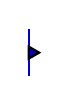
\begin{tikzpicture}[baseline=-0.5ex]
\draw [thick,blue!80!black] (0,2ex) -- (0,-2ex);
\draw [thick,fill=blue!80!black] (0,0.5ex) -- (0.866ex,0) -- (0,-0.5ex) -- cycle;
\end{tikzpicture}}}
\EnableCrossrefs
\CodelineIndex
\RecordChanges
\title{\pkg{beamer} named overlay specifications with \pkg{beanoves}}
\author{Jérôme Laurens}
\GetFileInfo{\jobname-debug.sty}
\date{\fileversion \qquad \filedate}
\NewDocumentEnvironment{BNVS.macrocode}{}{
  \setlength{\topsep}{0.4em plus 0.15 em minus 0.15 em}
  \leavevmode
  \begin{trivlist}
  \setlist[trivlist]{nosep}
  \item\vspace{-\baselineskip}
}{
  \end{trivlist}
}
\NewDocumentEnvironment{BNVS.workflow}{}{
  \begin{trivlist}
  \tabcolsep0ex
  \def\KWNstep{\llap{\smash{%
    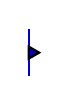
\begin{tikzpicture}[baseline=-0.5ex]
    \draw [thick,blue!80!black] (0,2ex) -- (0,-2ex);
    \draw [thick,fill=blue!80!black] (0,0.5ex) -- (0.866ex,0) -- (0,-0.5ex) -- cycle;
    \end{tikzpicture}%
    \hskip0.75ex
  }}}
  \item
  \begin{tabular}{ll}
}{
  \end{tabular}
  \end{trivlist}
}
\def\KWNmeta#1{\meta{\textsl{\nobreak#1\nobreak}}}%
\def\KWNmarg#1{\marg{\textsl{\nobreak#1\nobreak}}}%
\def\KWNsub#1{\raisebox{-0.5ex}{\scriptsize#1}}%
\NewDocumentEnvironment {BNVS.OnlyImplementation} {} {} {}%
\AddToHook{cmd/OnlyDescription/before}{
\RenewDocumentEnvironment {BNVS.OnlyImplementation} { +b } {} {}%
}%
%\OnlyDescription
%\typein{F000}
\begin{document}
\maketitle
\changes{v1.0}{2025/01/01}{First public release}
\begin{abstract}
This package allows the management of multiple named overlay specifications in \pkg{beamer} documents.
Named overlay specifications are very handy both during edition and
to manage complex and variable \pkg{beamer} overlay specifications.
In particular, they allow to replace raw numbers in \pkg{beamer}
|<...>| overlay specifications by logical identifiers.
Demonstration files are \href[pdfnewwindow]{https://github.com/jlaurens/beanoves/tree/main/demo}{available for download}
as part of the
\href[pdfnewwindow]{https://github.com/jlaurens/beanoves/}{development repository}.
This is a solution to this \href[pdfnewwindow]{https://latex.org/forum/viewtopic.php?t=25777}{\texttt{latex.org} forum query}.
\end{abstract}
%
\tableofcontents
%
\begin{documentation}
%
\section{Installation}
\subsection{Package manager}
When not already available, \pkg{beanoves} package
may be installed using a TEX distribution’s package manager,
either from the graphical user interface, or with the relevant command (|tlmgr| for \TeX\ Live and
|mpm| for MiK\TeX).
This should install files \pkg{beanoves.sty} and its debug version
\pkg{beanoves-debug.sty} as well as \pkg{beanoves-doc.pdf} documentation.

\subsection{Manual installation}
The \pkg{beanoves} source files are available from the \href[pdfnewwindow]{https://github.com/jlaurens/beanoves}{source repository}.
They can also be fetched from the \href[pdfnewwindow]{https://ctan.org/pkg/beanoves}{CTAN repository}.

\subsection{Usage}
The \pkg{beanoves} package is imported by putting \KWNlatex{\RequirePackage{beanoves}}
in the preamble of a \LaTeX\ document that uses the \pkg{beamer} class.
Should the package cause problems, 
its features can be temporarily deactivated with
simple commands "\BeanovesOff" and "\BeanovesOn".

\section{Minimal example}
%
The \LaTeX\ document below is a contrived example to show how the |beamer|
overlay specifications have been extended.
More demonstration files are available from the
\href[pdfnewwindow]{https://github.com/jlaurens/beanoves/tree/main/demo}{\pkg{beanoves} source repository}.
\begin{tcblisting} {
  listing only,
  listing file = example1.tex,
  minted options={
    fontsize=\small,
    breaklines,
    linenos,
    numbersep=0.5\baselineskip,
  },
  minted language=latex,
}
\documentclass{beamer}
\RequirePackage{beanoves}
\begin{document}
\Beanoves {
  A = 1:4,
  B = A.last::3,
  C = B.next,
}
\begin{frame}
  {\Large Frame \insertframenumber}
  {\Large Slide \insertslidenumber}
-- \visible<?(A.1)> {Only on slide 1}\\
-- \visible<?(B.range)> {Only on slides 4 to 6}\\
-- \visible<?(C.1)> {Only on slide 7}\\
-- \visible<?(A.2)> {Only on slide 2}\\
-- \visible<?(B.2:B.last)> {Only on slides 5 to 6}\\
-- \visible<?(C.2)> {Only on slide 8}\\
-- \visible<?(A.next)-> {From slide 5}\\
-- \visible<?(B.3:B.last)> {Only on slide 6}\\
-- \visible<?(C.3)> {Only on slide 9}\\
\end{frame}
\end{document}
\end{tcblisting}
%
On line 4, we use the |\Beanoves| command to declare \emph{named overlay sets}.
On line 5, we declare an overlay set named `A', which is a range starting at slide 1 and ending at slide 4.
On line 12, the extended \emph{named overlay specification} \texttt{?(A.1)} stands for 1 because 1 is the first index of the overlay set named A.
On line 15, \texttt{?(A.2)} stands for 2
whereas on line 18, \texttt{?(A.next)} stands for 5.
%
On line 6, we declare a second overlay set named `B',
starting after the 3 slides of `A' namely 4.
Its length is 3 meaning that its last slide number is 6,
thus each \texttt{?(B.last)} is replaced by 6.
The next slide number after slide range `B' is 7
which is also the start of the third slide range
due to line 7.
\section{Named overlay sets}
\subsection{Presentation}
Within a \pkg{beamer} frame, there are different slides that appear in turn
according to overlay specifications. The main overlay set is a range of integers
covering all the slide numbers, from one to the total amount of slides.
In general, an overlay set is a range of positive integers identified by a unique name.
The main practical interest is that such sets may be defined relative to one another, we can even have lists of overlay sets.
Finally, we can use these lists to build and organize \pkg{beamer} overlay
specifications logically.
\subsection{Named overlay reference}
|A.1|, |C.2| are \emph{named overlay references}, as well as |A| and |Y!C.2|.
More precisely, they are string identifiers, each one referencing
a well defined static integer or range to be used in \pkg{beamer} overlay specifications.
They have 3 components:
\begin{enumerate}
\item frame \texttt{\KWNmeta{id}!}, like |X!|, optional
\item \texttt{\KWNmeta{short name}} like |A|, required
\item \texttt{.\meta{\textsl{c}_1}....\meta{\textsl{c}_j}} like |.B.C|, optional (\(j=0\)), globally denoted as \emph{dotted path}.
\end{enumerate}
The \emph{frame ids}, \emph{short names} and \KWNmeta{c}'s
are alphanumerical case sensitive identifiers,
with possible underscores but with no space.
Unicode symbols above \texttt{U+00A0} are allowed if the underlying \TeX\ engine
supports it.
Only the \emph{frame id} is allowed to be empty, in which case it may apply to any common frame.
The \emph{short names} must not consist of only lowcase letters%
\footnote{This will avoid collisions with the "fp" module of "expl3".}.

The mapping from \emph{named overlay references} to sets of integers is defined
at the global \TeX\ level to allow its use in
\KWNlatex{\begin{frame}<...>}
and to share the same overlay sets between different frames.
Hence the \emph{frame id} due to the need to possibly target a particular frame.

\subsection{Defining named overlay sets}
In order to define \emph{named overlay sets}, we can either execute the next "\Beanoves" command  before a \pkg{beamer} \text{frame} environment, or use the custom |beanoves| option of this environment.
%
\begin{function}{\Beanoves, \Beanoves*}
  \begin{syntax}
    "\Beanoves"\{\meta{\textsl{ref}_1}=\meta{\textsl{spec}_1},...,\meta{\textsl{ref}_j}=\meta{\textsl{spec}_j}\}
  \end{syntax}
Each \KWNmeta{ref} key is a \emph{named overlay reference} whereas each \KWNmeta{spec} is an \emph{overlay set specifier}.
When the same \KWNmeta{ref} key is used multiple times, only the last one is taken into account.
%
\end{function}
When performed at the document level, the "\Beanoves" command starts by cleaning 
what was set by previous calls. When performed inside \LaTeX\ environments,
each new call cumulates with the previous one.
Notice that the argument of this function can contain macros:
they will be exhaustively expanded at resolution time\footnote{Precision is needed about the exact time when the expansion occurs.}.
\begin{function}{beanoves}
  \begin{syntax}
    beanoves = \{\meta{\textsl{ref}_1}=\meta{\textsl{spec}_1},...,\meta{\textsl{ref}_j}=\meta{\textsl{spec}_j}\}
  \end{syntax}
\end{function}
The "\Beanoves" arguments take precedence over both the "\Beanoves*" arguments
and the \texttt{beanoves} options. This allows to provide an overlay name
only when not already defined, which is helpfull when the very same frame source
is included multiple times in different contexts.
Notice that \texttt{\KWNmeta{ref}=1} can be shortened to \text{\KWNmeta{ref}}.
%
\subsubsection{Value specifiers}
\label{section:ValueSpecifiers}
Hereafter \KWNmeta{value} denotes a numerical expression.
\paragraph{Standalone}
\begin{description}
\item[\texttt{\KWNmeta{ref}=\KWNmeta{value}},]
a \emph{value specifier} for a single number.
When omitted it defaults to \(1\).
\end{description}

The numerical expressions are evaluated and then rounded using
"\fp_eval:n". They can contain mathematical functions and
\emph{named overlay references} defined above but should not
contain \emph{named overlay references} to \emph{value specifiers}.

The corresponding overlay set can be seen as a \emph{value counter}.


\subsubsection{Range specifiers}
Hereafter \KWNmeta{first}, \KWNmeta{last} and
\KWNmeta{length} are \emph{value specifiers}.
\paragraph{Standalone}
\begin{description}[noitemsep]
\item[\KWNmeta{ref}=\texttt{\KWNmeta{first}:},]
\item[\KWNmeta{ref}=\texttt{\KWNmeta{first}::},]
for the infinite range of signed integers starting at and including \KWNmeta{first}.
\end{description}
\begin{description}[noitemsep]
\item[\KWNmeta{ref}=\texttt{\KWNmeta{first}:\KWNmeta{last}},]
\item[\KWNmeta{ref}=\texttt{\KWNmeta{first}::\KWNmeta{length}},]
\item[\KWNmeta{ref}=\texttt{:\KWNmeta{last}::\KWNmeta{length}},]
\item[\KWNmeta{ref}=\texttt{::\KWNmeta{length}:\KWNmeta{last}},]
are variants for the same finite range of signed integers starting at and including \KWNmeta{first}, ending at and including \KWNmeta{last},
provided \(\KWNmeta{first}+\KWNmeta{length}=\KWNmeta{last}+1\).
\texttt{\KWNmeta{first}} can be omitted, in which case it defaults to \(1\).
Additionally \texttt{:\KWNmeta{last}}
and \texttt{::\KWNmeta{length}} are then equivalent.
\end{description}
\begin{description}[noitemsep]
\item[\KWNmeta{ref}=\texttt{:\KWNmeta{last}},]
\item[\KWNmeta{ref}=\texttt{::\KWNmeta{length}},]
are syntactic sugar when \KWNmeta{first} is \(1\).
\end{description}
\subsubsection{List specifiers}
\label{section:ListSpecifier}
\begin{description}
\item[\texttt{\KWNmeta{ref}=[\meta{\textsl{def}_1},...,\meta{\textsl{def}_j}]},]
\hypertarget{doc:BracketKeyval/range}{where}
\texttt{\meta{\textsl{def}_k}}, \(1≤k≤j\), is one of
\begin{itemize}
\item \KWNlatex{|\KWNmeta{index}|=|\KWNmeta{value}|},
\item \KWNlatex{|\KWNmeta{value}|}, a shortcut for \KWNlatex{|\KWNmeta{i}|=|\KWNmeta{value}|},
\KWNmeta{i} being the smallest positive integer such that \KWNlatex{|\KWNmeta{ref}|.|\KWNmeta{i}|}
is not already defined.
\end{itemize}
The first step is to remove previous \KWNmeta{ref} related definitions, then execute the various
\texttt{\KWNmeta{ref}.\KWNmeta{i}=\KWNmeta{value}}
definitions in the order given.
\begin{BNVS.OnlyImplementation}%
Here is the
\hyperlink{imp:BracketKeyval}{implementation}.
\end{BNVS.OnlyImplementation}
\item[\texttt{\KWNmeta{ref}=\{\meta{\textsl{def}_1},...,\meta{\textsl{def}_j}\}},]
\hypertarget{doc:BraceKeyval}{where}
\texttt{\meta{\textsl{def}_k}}, \(1≤k≤j\), is one of
\begin{itemize}
\item \texttt{\KWNmeta{name}=\KWNmeta{spec}},
\item \texttt{\KWNmeta{name}} for \texttt{\KWNmeta{name}=1},
\end{itemize}
The first step is to remove previous \KWNmeta{ref} related definitions, then execute the various
\KWNlatex{|\KWNmeta{ref}|.|\KWNmeta{name}|=|\KWNmeta{spec}|}
definitions in the order given.
In a final step, the \KWNmeta{name}'s are collected in a comma sepated list to
initialize \KWNmeta{ref} with.
\KWNmeta{spec} is any specifier.
\begin{BNVS.OnlyImplementation}%
Here is the
\hyperlink{imp:BraceKeyval}{implementation}.
\end{BNVS.OnlyImplementation}
\end{description}

\section{Resolution of \texttt{?(...)} query expressions}
This is the key feature of the \pkg{beanoves} package, extending \pkg{beamer} \emph{overlay specifications} normally included between pointed brackets. Before the \emph{overlay specifications} are processed by the \pkg{beamer} class,
the \pkg{beanoves} package scans them for any occurrence of
\KWNlatex{?(|\KWNmeta{queries}|)}. Each one is then evaluated and replaced
by its resolved static counterpart.
The overall result is finally forwarded to the \pkg{beamer} class.

The \KWNmeta{queries} argument is a comma separated list of individual \KWNmeta{query}'s processed from left to right as explained below.
Notice that nesting a \KWNlatex{?(|\KWNmeta{...}|)} query expression inside another
query expression is supported.

The named overlay sets defined above are queried for integer numerical values
that will be passed to \pkg{beamer}.
Turning an \emph{overlay query} into the static expression it represents,
as when above \texttt{?(A.1)} was replaced by \texttt{1}, is denoted by \emph{overlay query resolution} or simply \emph{resolution}.
The process starts by replacing any \emph{query reference} by its value as explained below until obtaining numerical expressions that are evaluated and finally rounded to the nearest integer to feed \pkg{beamer} with either ranges or numbers.
When the \emph{query reference} is a previously declared \texttt{\KWNmeta{ref}}, like |X| after |X=1|,
it is simply replaced by the corresponding declared
\texttt{\KWNmeta{value}}, here |1|.
Otherwise, we use \emph{implicit overlay queries} and their \emph{resolution rules} depending
on the definition of the named overlay set.
Hereafter \KWNmeta{i} denotes a signed integer whereas \KWNmeta{value},
\KWNmeta{first}, \KWNmeta{last}, \KWNmeta{length} and \KWNmeta{i expr}
stand for raw integers or more general numerical expressions that are
evaluated beforehands.

\emph{Resolution} occurs only when requested and the result is cached for
performance reason.

\subsection{Range overlay queries}
\label{section:ROQ}
\begin{description}
\item[\texttt{\KWNmeta{ref} = \KWNmeta{first}:}] as well as \texttt{\KWNmeta{first}::}
define a range limited from below:
\begin{center}
\begin{tabular}{>{ \ttfamily \bfseries }l|>{ \ttfamily }l}
\hline
\bfseries \textrm{overlay query} & \bfseries \textrm{resolution} 
\\\hline
\KWNmeta{ref}   & \KWNmeta{first}-\\
\KWNmeta{ref}.1 & \KWNmeta{first}\\
\KWNmeta{ref}.2 & \(\KWNmeta{first}+1\) \\
\KWNmeta{ref}.\KWNmeta{i} & \(\KWNmeta{first} + \KWNmeta{i} - 1\) \\
\KWNmeta{ref}.previous & \(\KWNmeta{first}-1\)\\
\KWNmeta{ref}.first & \(\KWNmeta{first}\)\\
\hline
\end{tabular}
\end{center}
Notice that \texttt{\KWNmeta{ref}.previous} and \texttt{\KWNmeta{ref}.0} are most of the time synonyms.
\item[\texttt{\KWNmeta{ref} = \KWNmeta{first}:\KWNmeta{last}}]
as well as variants \texttt{\KWNmeta{first}::\KWNmeta{length}},
\texttt{::\KWNmeta{length}:\KWNmeta{last}}
or \texttt{:\KWNmeta{last}::\KWNmeta{length}},
which are equivalent provided \(\KWNmeta{first}+\KWNmeta{length} = \KWNmeta{last}+1\).

Define a range limited from both above and below:
\begin{center}
\begin{tabular}{>{ \ttfamily \bfseries }l|>{ \ttfamily }l}
\hline
\bfseries \textrm{overlay query} & \bfseries \textrm{resolution} 
\\\hline
\KWNmeta{ref} & \KWNmeta{first}-\KWNmeta{last}\\
\KWNmeta{ref}.1 & \(\KWNmeta{first}\)\\
\KWNmeta{ref}.2 & \(\KWNmeta{first}+1\) \\
\KWNmeta{ref}.\KWNmeta{i} & \(\KWNmeta{first} + \KWNmeta{\textsl{i}} - 1\) \\
\KWNmeta{ref}\{\KWNmeta{i expr}\} & \(\KWNmeta{first} + \KWNmeta{i expr} - 1\) \\
\KWNmeta{ref}.previous & \(\KWNmeta{first}-1\)\\
\KWNmeta{ref}.first & \(\KWNmeta{first}\)\\
\KWNmeta{ref}.last & \(\KWNmeta{last}\)\\
\KWNmeta{ref}.next & \(\KWNmeta{last}+1\)\\
\KWNmeta{ref}.length & \(\KWNmeta{length}\)\\
\hline
\end{tabular}
\end{center}
Notice that the resolution of the \texttt{\KWNmeta{ref}} overlay query
is a \pkg{beamer} range and not an algebraic difference,
negative integers do not make sense there while in \pkg{beamer} context.

In the frame example below, we use the
\mintinline{latex}{\BeanovesResolve} command for the demonstration.
It is mainly used for debugging and testing purposes.

\begin{tcblisting} {
  listing only,
  minted options={
    fontsize=\small,
    breaklines,
    linenos,
    numbersep=0.5\baselineskip,
    escapeinside=||
  },
  minted language=latex,
}
\Beanoves {
| | A = 3:8, % or similarly A = 3::6, A = ::6:8 and A = :8::6
}
\begin{frame} {Frame \insertframenumber} {Slide \insertslidenumber}
\ttfamily
\BeanovesResolve[show](A)          == 3-8,
\BeanovesResolve[show](A.1)        == 3,
\BeanovesResolve[show](A.-1)       == 1,
\BeanovesResolve[show](A.previous) == 2,
\BeanovesResolve[show](A.first)    == 3,
\BeanovesResolve[show](A.last)     == 8,
\BeanovesResolve[show](A.next)     == 9,
\BeanovesResolve[show](A.length)   == 6,
\end{frame}
\end{tcblisting}
%
\end{description}
\begin{description}[noitemsep]
\item[\texttt{\KWNmeta{ref} = [...]}]
\item[\texttt{\KWNmeta{ref} = \{...\}}]
See the list range specifiers in section \ref{section:ListSpecifier}.
\end{description}
%
\subsection{Value counter queries}
\label{section:counter}
\begin{description}
\item[\texttt{\KWNmeta{ref} = \KWNmeta{value}}] defines a counter value.
\begin{center}
\begin{tabular}{>{ \ttfamily \bfseries }l|>{ \ttfamily }l}
\hline
\bfseries \textrm{overlay query} & \bfseries \textrm{resolution} 
\\\hline
\KWNmeta{ref}   & \(\KWNmeta{value}\)\\
\KWNmeta{ref}.1 & \(\KWNmeta{value}\)\\
\KWNmeta{ref}.2 & \(\KWNmeta{value}+1\) \\
\KWNmeta{ref}.\KWNmeta{i} & \(\KWNmeta{value} + \KWNmeta{i} - 1\) \\\KWNmeta{ref}\{\KWNmeta{i expr}\} & \(\KWNmeta{value} + \KWNmeta{i expr} - 1\) \\
\KWNmeta{ref}.previous & \(\KWNmeta{value}-1\)\\
\KWNmeta{ref}.first & \(\KWNmeta{value}\)\\
\KWNmeta{ref}.last & \(\KWNmeta{value}\)\\
\KWNmeta{ref}.next & \(\KWNmeta{value}+1\)\\
\hline
\end{tabular}
\end{center}
\end{description}
Additionnaly, resolution rules are provided for dedicated \emph{overlay queries}. Here, \KWNmeta{ref} is considered a standard programming variable:
\begin{description}
\item[\texttt{\KWNmeta{ref}=\KWNmeta{integer expression}},] resolve \KWNmeta{integer expression} into \KWNmeta{integer}, assign it to the \KWNmeta{ref} and use it.
It defines \KWNmeta{ref} globally if not already done.
Here \KWNmeta{integer expression} is the longest character sequence with no space%
\footnote{The parser for algebraic expression is very rudimentary.}.
\item[\texttt{\KWNmeta{ref}+=\KWNmeta{integer expression}},] resolve \KWNmeta{integer expression} into \KWNmeta{integer}, advance \KWNmeta{ref} by \KWNmeta{integer} and use the result.
\item[\texttt{++\KWNmeta{ref}},] increment \KWNmeta{ref} by \(1\) and use it.
\item[\texttt{\KWNmeta{ref}++},] use \KWNmeta{ref} and then increment it by \(1\).
\end{description}

This can be used for an indirection.
\marginpar{\textbf{\color{red}IN PROGRESS}}
\begin{tcblisting} {
  listing only,
  minted options={
    fontsize=\small,
    breaklines,
    linenos,
    numbersep=0.5\baselineskip,
    escapeinside=||
  },
  minted language=latex,
}
\Beanoves {
|  |A = 1,
|  |B = [ 10 = 100 ],
|  |C = 10,
}
\begin{frame} {Frame \insertframenumber} {Slide \insertslidenumber}
\ttfamily
\BeanovesResolve[show](A.C)      == \BeanovesResolve[show](A.10) == 10,
\BeanovesResolve[show](B.C)      == \BeanovesResolve[show](B.10) == 100,
\BeanovesResolve[show](A[C+=10]) == \BeanovesResolve[show](A.20) == 20,
\BeanovesResolve[show](A.C)      == \BeanovesResolve[show](A.20) == 20,
\BeanovesResolve[show](A.C+=10)  == \BeanovesResolve[show](A.20) == 20+10,
\BeanovesResolve[show](A.C)      == \BeanovesResolve[show](A.20) == 30,
\BeanovesResolve[show](B.C)      == \BeanovesResolve[show](B.20) == 20,
\end{frame}
\end{tcblisting}

In order to decrement a counter, one can increment with a negative value, no dedicated syntax is provided yet.

For each new frame, these counters are reset to the value
they were initialized with. Sometimes, resetting the counter
manually is necessary, for example when managing \pkg{tikz} overlay material.
%
\begin{function}{\BeanovesReset}
  \begin{syntax}
    "\BeanovesReset" \oarg{\textsl{options}} \{\meta{\textsl{ref}_1}[=\meta{\textsl{spec}_1}],..., \meta{\textsl{ref}_j}[=\meta{\textsl{spec}_j}]\}
  \end{syntax}
This command is very similar to \KWNlatex{\Beanoves},
except that a standalone \texttt{\meta{\textsl{ref}_i}} resets the counter to
the last value it was initialized with, and that it is meant to be used inside a
\texttt{frame} environment. When the \texttt{all} option is provided,
some internals that were cached for performance reasons are cleared
as well.
\end{function}
%
\subsection{The \texttt{beamer} counters}
While inside a \texttt{frame} environment,
it is possible to save the current value of the \texttt{beamerpauses} counter that controls whether elements should appear on the current slide.
For that, we can execute one of \KWNlatex{\Beanoves{|\KWNmeta{ref}|=pauses}} or in a query
\KWNlatex{?(...(|\KWNmeta{ref}|=pauses)...)}.
Then later on, we can use |?(...|\KWNmeta{ref}|...)| to refer to this saved value
in the same frame\footnote{See
\href[pdfnewwindow]{https://tex.stackexchange.com/questions/34458/reference-overlay-numbers-with-names}{stackexchange}
for an alternative that needs at least two passes.}.
Next frame source is an example of usage.
\begin{tcblisting} {
  listing only,
  minted options={
    fontsize=\small,
    breaklines,
    linenos,
    numbersep=0.5\baselineskip,
  },
  minted language=latex,
}
\begin{frame}
\visible<+->{A}\\
\visible<+->{B\Beanoves{afterB=pauses}}\\
\visible<+->{C}\\
\visible<?(afterB)>{other C}\\
\visible<?(afterB.previous)>{other B}\\
\end{frame}
\end{tcblisting}
``A'' first appears on slide 1, ``B'' on slide 2 and ``C'' on slide 3.
On line 2, |afterB| takes the value of the \texttt{beamerpauses}
counter once updated, \emph{id est} 3.
``B'' and ``other B'' as well as ``C'' and ``other C'' appear at the same time.
%
If the |beamerpauses| counter is not suitable,
we can execute instead one of \KWNlatex{\Beanoves{|\KWNmeta{ref}|=slideinframe}} or inside a query
\KWNlatex{?(|\KWNmeta{...}|(|\KWNmeta{ref}|=slideinframe)|\KWNmeta{...}|)}.
It uses the numerical value of
\KWNlatex{\insertslideinframe}.

\subsection{Multiple queries}
It is possible to replace the comma separated list of queries
\KWNlatex{?(|\meta{\textsl{query}_1}|),}...\KWNlatex{,?(|\meta{\textsl{query}_j}|)}
with the shorter single query
\KWNlatex{?(|\meta{\textsl{query}_1}|,}...\KWNlatex{,|\meta{\textsl{query}_j}|)}.
%
\subsection{Frame id}
Except for very special situations, the \emph{frame ids} can be left unspecified.
When no \emph{frame id} was explicitly provided,
\pkg{beanoves} uses the \emph{last frame id} and if the resolution fails
an empty \emph{frame id}. At the beginning of each frame,
the \emph{last frame id} is set to the \emph{frame id} of the current frame,
which is denoted \emph{current frame id} and is empty by default.
Then it gets updated after each named reference resolution where a
\emph{frame id} is explicitly given.
For example, the first time |A.1| reference is resolved within a given frame,
it is first translated to \texttt{\KWNmeta{last frame id}!A.1},
but when used just after \texttt{Y!C.2}, for example, it becomes a shortcut to
\texttt{Y!A.1} because the \emph{last frame id} is then \texttt{Y}.

In order to set the \emph{frame id} of the current frame to frame \KWNmeta{id},
use the new \texttt{beanoves id} option of the \pkg{beamer} frame environment. 
\begin{function}{beanoves id}
  \begin{syntax}
    beanoves id=frame \KWNmeta{id},
  \end{syntax}
\end{function}
We can use the same frame \KWNmeta{id} for different frames to share named overlay sets.
Another possibility offered by the \pkg{beanoves} package to share named
overlay sets is a fall back mechanism, for example when
\KWNlatex{X!A} cannot be resolved, resolve \KWNlatex{!A} instead.
%
\subsection{Resolution command}
\begin{function}{\BeanovesResolve}
  \begin{syntax}
    "\BeanovesResolve" \oarg{\textsl{setup}} \marg{\textsl{queries}}
  \end{syntax}
This function resolves the \KWNmeta{queries},
which are like the argument of
\KWNlatex{?(|\KWNmeta{...}|)} instructions:
a comma separated list of single \KWNmeta{query}'s.
The optional \KWNmeta{setup} is a key--value:
\begin{itemize}
\item[\texttt{show}] the result is left into the input stream
\item[\texttt{in:N=\KWNmeta{command}}] the result is stored into \KWNmeta{command}.
\end{itemize}
\end{function}
%
\section{Support}
See the \href[pdfnewwindow]{https://github.com/jlaurens/beanoves}{source repository}.
One can report issues there.

\end{documentation}
\DocInput{beanoves.dtx}
\begin{luacode}
local bnvs = require("./\jobname-test.lua")
tex.print("\\BNVSNote{".. bnvs.__INFO__.."}%")
local ra = bnvs.check_variants("\jobname.sty")
tex.print("\\BNVSNote{"..table.concat(ra, "^^J").."}")
--[[
if ra then
  for _,v in ipairs(ra) do
    tex.print("\\verb|"..v.."|\\\\")
  end
end
]]
\end{luacode}
\end{document}
%</driver>
% \fi
%
%\StopEventually{^^A
%  \PrintChanges
%  \PrintIndex
%}
%
% \NewDocumentEnvironment {BNVS.gobble} { +b } {} {}
% \begin{implementation}
% \begin{BNVS.gobble}
%<*package>
% \end{BNVS.gobble}
%
%\begin{BNVS.gobble}
%\begin{luacode}
%local bnvs = require("./\jobname-test.lua")
%tex.print("\\BNVSNote{".. bnvs.__INFO__.."}%")
%local ra = bnvs.check_variants("\jobname-debug.sty")
%tex.print("\\BNVSNote{"..table.concat(ra, "^^J").."}")
%--[[
%if ra then
%  for _,v in ipairs(ra) do
%    tex.print("\\verb|"..v.."|\\\\")
%  end
%end
%]]
%\end{luacode}
%\end{BNVS.gobble}
%
%
% \section{Implementation}
%
% Identify the internal prefix (\LaTeX3 \pkg{DocStrip} convention).
% \begin{BNVS.macrocode}
%    \begin{macrocode}
%<@@=bnvs>
%    \end{macrocode}
% \end{BNVS.macrocode}
%
% \subsection{Package declarations}
%
% \begin{BNVS.macrocode}
%    \begin{macrocode}
\NeedsTeXFormat{LaTeX2e}[2020/01/01]
\ProvidesExplPackage
%    \end{macrocode}
% \begin{BNVS.gobble}
%<*!debug>
% \end{BNVS.gobble}
%    \begin{macrocode}
  {beanoves}
%    \end{macrocode}
% \begin{BNVS.gobble}
%</!debug>
%<*!final>
  {beanoves-debug}
%</!final>
% \end{BNVS.gobble}
%    \begin{macrocode}
  {2024/01/11}
  {1.0}
  {Named overlay specifications for beamer}
%    \end{macrocode}
% \end{BNVS.macrocode}
%
% \subsection{Overview}
% Reserved namespace:
% identifiers containing the case insensitive string |beanoves| or
% containing the case insensitive string |bnvs| delimited by two non characters.
%
% There are mainly two steps: parsing and resolution.
% Parsing occurs while executing the \KWNlatex{\Beanoves} command
% to build a data model whereas the resolution translates queries into
% \pkg{beamer} specifications based on this data model.
%
% The development is easier due to a facility layer over \pkg{expl}.
% 
% \subsection{Facility layer: definitions and naming}
% In order to make the code shorter and easier to read during development, we add a layer
% over \LaTeX3. The |c| and |v| argument specifiers take a slightly different meaning when
% used in a function which name contains |bnvs| or |BNVS|.
% Where \LaTeX3 would transform |l__bnvs_ref_tl| into |\l__bnvs_ref_tl|,
% \pkg{bnvs} will directly transform |ref| into |\l__bnvs_ref_tl|.
% The type of the local variable used depends on the context and may be
% |seq| or |int| for example.
% There are however a pair of exceptions mentionned below.
% For a better reading experience,
% ``|ref|'' will generally stand for |\l__bnvs_ref_tl|,
% whereas ``|path| sequence'' will generally stand for |\l__bnvs_path_seq|.
% Other similar shortcuts are used as well. 
%
% Functions with |BNVS| in their names are management functions.
% They belong to a deeper layer and do not contain any logic specific
% to the \pkg{beanoves} package.
% \begin{function}{
%   \BNVS:c,
%   \BNVS_l:cn,
%   \BNVS_g:cn,
% }
% \begin{syntax}
% "\BNVS:c" \KWNmarg{cs core name}
% "\BNVS_l:cn" \KWNmarg{local variable core name} \KWNmarg{type}
% "\BNVS_g:cn" \KWNmarg{global variable core name} \KWNmarg{type}
% \end{syntax}
% These are naming functions internally used to focus on the discrimining part
% of variable or function names.
% \end{function}
% \begin{BNVS.macrocode}
%    \begin{macrocode}
\cs_new:Npn \BNVS:c    #1    { __bnvs_#1     }
\cs_new:Npn \BNVS_l:cn #1 #2 { l__bnvs_#1_#2 }
\cs_new:Npn \BNVS_g:cn #1 #2 { g__bnvs_#1_#2 }
%    \end{macrocode}
% \end{BNVS.macrocode}
% \begin{function}{
%   \BNVS_use_raw:N,
%   \BNVS_use_raw:c,
%   \BNVS_use_raw:Nc,
%   \BNVS_use_raw:nc,
%   \BNVS_use:c,
%   \BNVS_use:Nc,
%   \BNVS_use:nc,
% }
% \begin{syntax}
% "\BNVS_use_raw:N" \KWNmeta{cs}
% "\BNVS_use_raw:c" \KWNmarg{cs name}
% "\BNVS_use_raw:Nc" \KWNmeta{function} \KWNmarg{cs name}
% "\BNVS_use_raw:nc" \KWNmarg{tokens} \KWNmarg{cs name}
% "\BNVS_use:c" \KWNmarg{cs core}
% "\BNVS_use:Nc" \KWNmeta{function} \KWNmarg{cs core}
% "\BNVS_use:nc" \KWNmarg{tokens} \KWNmarg{cs core}
% \end{syntax}
% "\BNVS_use_raw:c" is a convenient wrapper over "\use:c".
% possibly prepended with some code, for debugging and testing.
% It needs 3 expansion steps just like "\BNVS_use:c".
% The other are used to expand "\use:c" enough before usage by
% \KWNmeta{function} or \KWNmeta{tokens}.
% The first argument of \KWNmeta{function} has type |N|.
% The next token after \KWNmeta{tokens} will have type |N| too.
% \KWNmeta{cs name} is a full cs name
% whereas \KWNmeta{cs core} will be prepended with the appropriate prefix
% specific to the \pkg{beanoves} package.
% \end{function}
% \begin{BNVS.macrocode}
%    \begin{macrocode}
\cs_new:Npn \BNVS_use_raw:N #1 { #1 }
\cs_new:Npn \BNVS_use_raw:c #1 {
  \exp_last_unbraced:No
  \BNVS_use_raw:N { \cs:w #1 \cs_end: }
}
%    \end{macrocode}
% \begin{BNVS.test}{:N=\BNVS_use_raw:N, noigre}
% \tl_clear:N \l__bnvs_TEST_A_tl
% \exp_args:NNo \tl_set:Nn \l__bnvs_TEST_A_tl { \BNVS_use_raw:N \BNVS: }
% \tl_if_in:NnF \l__bnvs_TEST_A_tl { \BNVS: } {
%   \typeout{\tl_to_str:V \l__bnvs_TEST_A_tl}
%   \test_fail:n A
% }
% \end{BNVS.test}
% \end{BNVS.macrocode}
% \begin{BNVS.macrocode}
%    \begin{macrocode}
\cs_new:Npn \BNVS_use:c #1 {
  \BNVS_use_raw:c { \BNVS:c { #1 } }
}
%    \end{macrocode}
% \end{BNVS.macrocode}
% \begin{BNVS.test}{:N=\BNVS_use:c, ignore}
% \BNVS_new:cpn { TEST:n } #1 { #1#1 }
% \tl_set:Nx \l__bnvs_TEST_tl { \BNVS_use:c { TEST:n } { X } }
% \tl_if_eq:NnF \l__bnvs_TEST_tl { XX } { 
%   \test_fail:n { NO_WAY }
% }
% \BNVS_undefine:c { TEST:n }
% \end{BNVS.test}
% \begin{BNVS.macrocode}
%    \begin{macrocode}
\cs_new:Npn \BNVS_use_raw:NN #1 #2 {
  #1 #2
}
%    \end{macrocode}
% \end{BNVS.macrocode}
% \begin{BNVS.macrocode}
%    \begin{macrocode}
\cs_new:Npn \BNVS_use_raw:nN #1 #2 {
  #1 #2
}
%    \end{macrocode}
% \end{BNVS.macrocode}
% \begin{BNVS.macrocode}
%    \begin{macrocode}
\cs_new:Npn \BNVS_use_raw:Nc #1 #2 {
  \exp_args:NNc \BNVS_use_raw:NN #1 { #2 }
}
%    \end{macrocode}
% \begin{BNVS.test}{:N=\BNVS_use_raw:Nc, ignore}
% \exp_args:NNNo \exp_args:NNo \tl_set:No
%   \l__bnvs_TEST_tl { \BNVS_use_raw:Nc \BNVS:N { BNVS: } }
% \tl_if_eq:NnF \l__bnvs_TEST_tl { \BNVS:N \BNVS: } { 
%   \test_fail:n { NO_WAY }
% }
% \end{BNVS.test}
% \end{BNVS.macrocode}
% \begin{BNVS.macrocode}
%    \begin{macrocode}
\cs_new:Npn \BNVS_use_raw:nc #1 #2 {
  \exp_last_unbraced:Nno
  \BNVS_use_raw:nN { #1 } { \cs:w #2 \cs_end: }
}
%    \end{macrocode}
% \end{BNVS.macrocode}
% \begin{BNVS.macrocode}
%    \begin{macrocode}
\cs_new:Npn \BNVS_use:Nc #1 #2 {
  \BNVS_use_raw:Nc #1 { \BNVS:c { #2 } }
}
%    \end{macrocode}
% \end{BNVS.macrocode}
% \begin{BNVS.macrocode}
%    \begin{macrocode}
\cs_new:Npn \BNVS_use:nc #1 #2 {
  \BNVS_use_raw:nc { #1 } { \BNVS:c { #2 } }
}
%    \end{macrocode}
% \begin{BNVS.gobble}
%<*!final>
\cs_set_eq:NN \BNVS_use_raw_saved:N \BNVS_use_raw:N
\cs_set:Npn \BNVS_use_raw:N #1 {
  \cs_if_exist:NF #1 {
    \BNVS_fatal:x { Unknown~command~\token_to_str:N #1~(c) }
  }
  #1
}
\cs_set_eq:NN \BNVS_use_raw_saved:NN \BNVS_use_raw:NN
\cs_set:Npn \BNVS_use_raw:NN #1 #2 {
  \cs_if_exist:NF #2 {
    \BNVS_fatal:x { Unknown~command~\token_to_str:N #2~(N) }
  }
  \BNVS_use_raw_saved:NN #1 #2
}
\cs_set_eq:NN \BNVS_use_raw_saved:nN \BNVS_use_raw:nN
\cs_set:Npn \BNVS_use_raw:nN #1 #2 {
  \cs_if_exist:NF #2 {
    \BNVS_fatal:x { Unknown~command~\token_to_str:N #2~(use_raw:nN) }
  }
  \BNVS_use_raw_saved:nN { #1 } #2
}
%</!final>
% \end{BNVS.gobble}
% \begin{BNVS.test}{:N=\BNVS_use_raw:N, noigre}
% \cs_set:Npn \BNVS_fatal:x #1 #2 { \tl_set:Nn \l__bnvs_TEST_A_tl { FIASKO } }
% \BNVS_use_raw:N \BNVS_test:
% \tl_if_eq:NnF \l__bnvs_TEST_A_tl { FIASKO } {
%   \test_fail:n A
% }
% \end{BNVS.test}
% \begin{BNVS.test}{:N=\BNVS_tl_use:Nc, ignore}
% \cs_new:Npn \BNVS_test:N #1 {
%   \tl_if_eq:nnF { #1 } { \l__bnvs_TEST_tl } {
%     \test_fail:x { NO_WAY \token_to_str:N #1 }
%   }
% }
% \BNVS_tl_use:Nc \BNVS_test:N { TEST }
% \end{BNVS.test}
% \begin{BNVS.test}{:N=\BNVS_tl_use:nc, ignore}
% \cs_new:Npn \BNVS_test:N #1 {
%   \tl_if_eq:nnF { #1 } { \l__bnvs_TEST_tl } {
%     \test_fail:x {
%       ^^J=>\token_to_str:N #1
%       ^^J=>\tl_to_str:N #1
%       ^^J NO~WAY
%     }
%   }
% }
% \BNVS_tl_use:nc { \BNVS_test:N } { TEST }
% \prg_do_nothing:
% \end{BNVS.test}
% \begin{BNVS.test}{:N=\BNVS_tl_use:nv, ignore}
% \tl_set:Nn \l__bnvs_TEST_tl { SUCCESS }
% \cs_new:Npn \BNVS_test:n #1 {
%   \tl_if_eq:NnF \l__bnvs_TEST_tl { #1 } {
%     \test_fail:x {
%       ^^J=>\tl_to_str:N \l__bnvs_TEST_tl
%       ^^J=>\tl_to_str:n { #1 }
%       ^^J NO~WAY
%     }
%   }
% }
% \BNVS_tl_use:nv { \BNVS_test:n } { TEST }
% \prg_do_nothing:
% \end{BNVS.test}
% \end{BNVS.macrocode}
% \begin{BNVS.macrocode}
%    \begin{macrocode}
\tl_new:N \l__bnvs_last_unbraced_tl
\cs_new:Npn \BNVS_tl_last_unbraced:nv #1 {
  \tl_set:Nn \l__bnvs_last_unbraced_tl { #1 }
  \BNVS_tl_use:nc { \exp_last_unbraced:NV \l__bnvs_last_unbraced_tl }
}
%    \end{macrocode}
% \begin{BNVS.test}{:N=\BNVS_tl_last_unbraced:nv, ignore}
% \__bnvs_tl_set:cn { ans } { { SUCCESS } }
% \BNVS_tl_use:nv { \__bnvs_tl_set:cn { ans } } { ans }
% \assert_equal_ans:nn { { SUCCESS } } A
% \__bnvs_tl_set:cn { ans } { { SUCCESS } }
% \BNVS_tl_last_unbraced:nv { \__bnvs_tl_set:cn { ans } } { ans }
% \assert_equal_ans:nn { SUCCESS } B
% \end{BNVS.test}
%    \begin{macrocode}
\cs_new:Npn \BNVS_tl_use:nvv #1 #2 {
  \BNVS_tl_use:nv { \BNVS_tl_use:nv { #1 } { #2 } }
}
\cs_new:Npn \BNVS_tl_use:nvvv #1 #2 {
  \BNVS_tl_use:nvv { \BNVS_tl_use:nv { #1 } { #2 } }
}
%    \end{macrocode}
% \begin{BNVS.test}{:N=\BNVS_use_raw:c, ignore}
% \tl_clear:N \l__bnvs_TEST_tl
% \cs_set:Npn \BNVS_test: { SUCCESS }
% \tl_set:Nx \l__bnvs_TEST_tl { \BNVS_test: }
% \assert_equal_tl:vnn { TEST } { SUCCESS } { A }
% \tl_clear:N \l__bnvs_TEST_tl
% \tl_set:Nx \l__bnvs_TEST_tl { \BNVS_use_raw:c { BNVS_test: } }
% \assert_equal_tl:vnn { TEST } { SUCCESS } { A' }
% \tl_clear:N \l__bnvs_TEST_tl
% \cs_set:Npn \BNVS_fatal:x #1 {
%   \tl_set:Nn \l__bnvs_TEST_tl { FAILURE }
% }
% \BNVS_use_raw:c { BNVS_test: }
% \assert_equal_tl:vnn { TEST } { FAILURE } { B }
% \end{BNVS.test}
% \begin{BNVS.test}{:Nn=\BNVS_use:Nc{/:nc}, ignore}
% \BNVS_new:cpn { TEST: } { SUCCESS }
% \cs_if_exist:cF { \BNVS:c { TEST: } } {
%   \BNVS_fatal:x { Unknown~bnvs~command~TEST:~(ii-N) }
% }
% \cs_set:Npn \BNVS_test:N #1 {
%   \exp_args:No \tl_if_eq:nnF { #1 } { SUCCESS } {
%     \test_fail:x { E / \token_to_str:N #1 / }
%   }
% }
% \BNVS_use:Nc   \BNVS_test:N   { TEST: }
% \BNVS_use:nc { \BNVS_test:N } { TEST: }
% \BNVS_undefine:c { TEST: }
% \BNVS_set:cpn { TEST: } { SUCCESS }
% \cs_set:Npn \BNVS_test:N #1 {
%   \cs_if_eq:NNF #1 \__bnvs_TEST: {
%     \test_fail:x { TEST / \token_to_str:N #1 }
%   }
% }
% \BNVS_use:Nc   \BNVS_test:N   { TEST: }
% \BNVS_use:nc { \BNVS_test:N } { TEST: }
% \BNVS_undefine:c { TEST: }
% \end{BNVS.test}
% \end{BNVS.macrocode}
% \begin{BNVS.macrocode}
%    \begin{macrocode}
\cs_new:Npn \BNVS_log:n #1 { }
\cs_generate_variant:Nn \BNVS_log:n { x }
%    \end{macrocode}
% \end{BNVS.macrocode}
% ^^A
% \subsubsection{Debug}
% \begin{function}{
%   \BNVS_DEBUG_on:,
%   \BNVS_DEBUG_off:,
%   \BNVS_DEBUG_push:nn,
%   \BNVS_DEBUG_pop:,
% }
% \begin{syntax}
% "\BNVS_DEBUG_on:"
% "\BNVS_DEBUG_off:"
% "\BNVS_DEBUG_push:nn" \KWNmarg{types on} \KWNmarg{types off}
% "\BNVS_DEBUG_pop:"
% \end{syntax}
% These functions activate or deactivate the debug mode.
% They are only active in the \pkg{beanoves-debug} package.
% Manage debug messaging for one given \KWNmeta{type} or \KWNmeta{types}.
% The implementation is not publicly exposed.
% The \KWNmeta{type} is a single letter of \KWNlatex{**}.
% \end{function}
% \begin{BNVS.gobble}
% Defines |\BNVS_DEBUG_|\texttt{\KWNmeta{type}}|_log:n|
% and its |:x| variant.
% "\BNVS_DEBUG_on:n" creates the command \cs{BNVS_DEBUG_\KWNmeta{type}_log:n}
% for each \KWNmeta{type} in \KWNmeta{types}.
% \end{BNVS.gobble}
% \begin{BNVS.gobble}
%    \begin{macrocode}
%<*!debug>
\cs_new:Npn \BNVS_DEBUG_warning: {
  \BNVS_warning:n { Only~available~in~beanoves-debug~package. }
  \cs_set:Npn \BNVS_DEBUG_warning: {}
}
\cs_new:Npn \BNVS_DEBUG_on:n #1 {
  \BNVS_DEBUG_warning:
}
\cs_new:Npn \BNVS_DEBUG_off:n #1 {
  \BNVS_DEBUG_warning:
}
\cs_new:Npn \BNVS_DEBUG_push:n #1 {
  \BNVS_DEBUG_warning:
}
\cs_new:Npn \BNVS_DEBUG_push:nn #1 #2 {
  \BNVS_DEBUG_warning:
}
\cs_new:Npn \BNVS_DEBUG_pop: {
  \BNVS_DEBUG_warning:
}
\cs_new:Npn \BNVS_DEBUG_on: {
  \BNVS_DEBUG_warning:
}
\cs_new:Npn \BNVS_DEBUG_off: {
  \BNVS_DEBUG_warning:
}
%</!debug>
%<*!final>
\tl_const:Nn \c__BNVS_DEBUG_log_tl { CDBGpfarsRomqibSTHw* }
\cs_new:Npn \BNVS_DEBUG:c #1 {
  BNVS_DEBUG~#1~
}
\cs_new:Npn \BNVS_DEBUG_log_on:n  { \BNVS_log:n }
\cs_new:Npn \BNVS_DEBUG_on:nT #1 #2 {
  \tl_if_empty:nT { #1 } {
    \typein { Empty~argument~not~allowed }
  }
  \exp_args:Nc \token_if_eq_meaning:NNF { \BNVS_DEBUG:c { #1 } log:n } \BNVS_DEBUG_log_on:n {
    \cs_set_eq:cN { \BNVS_DEBUG:c { #1 } log:n } \BNVS_DEBUG_log_on:n
    \cs_generate_variant:cn { \BNVS_DEBUG:c { #1 } log:n } { x }
    #2
  }
}
\cs_new:Npn \BNVS_DEBUG_on:n #1 {
  \BNVS_DEBUG_on:nT { #1 } { }
}
\cs_new:Npn \BNVS_DEBUG_off:nT #1 #2 {
  \tl_if_empty:nT { #1 } {
    \typein { Empty~argument~not~allowed }
  }
  \exp_args:Nc \token_if_eq_meaning:NNT { \BNVS_DEBUG:c { #1 } log:n } \BNVS_DEBUG_log_on:n {
    \cs_set:cpn { \BNVS_DEBUG:c { #1 } log:n } { \use_none:n }
    #2
  }
}
\cs_new:Npn \BNVS_DEBUG_off:n #1 {
  \BNVS_DEBUG_off:nT { #1 } { }
}
\seq_new:N \l__bnvs_DEBUG_push_n_seq
% #1: what is added
% #2: what is removed
\tl_new:N \l__bnvs_DEBUG_push_nn_tl
\cs_new:Npn \BNVS_DEBUG_push:nn #1 #2 {
  \tl_if_eq:nnTF { #1 } { ** } {
    \exp_args:NV \tl_map_inline:nn \c__BNVS_DEBUG_log_tl
  } {
    \tl_map_inline:nn { #1 }
  }
  {
    \BNVS_DEBUG_on:nT { ##1 } {
      \tl_put_right:Nn \l__bnvs_DEBUG_push_nn_tl {
        \BNVS_DEBUG_off:n { ##1 }
      }
    }
  }
  \tl_if_eq:nnTF { #2 } { ** } {
    \exp_args:NV \tl_map_inline:nn \c__BNVS_DEBUG_log_tl
  } {
    \tl_map_inline:nn { #2 }
  }
  {
    \BNVS_DEBUG_off:nT { ##1 } {
      \tl_put_right:Nn \l__bnvs_DEBUG_push_nn_tl {
        \BNVS_DEBUG_on:n { ##1 }
      }
    }
  }
  \seq_put_left:NV \l__bnvs_DEBUG_push_n_seq \l__bnvs_DEBUG_push_nn_tl
  \tl_clear:N \l__bnvs_DEBUG_push_nn_tl
}
\cs_new:Npn \BNVS_DEBUG_push:n #1 {
  \tl_if_empty:nT { #1 } {
    \typein { Empty~argument~not~allowed }
  }
  \BNVS_DEBUG_push:nn { #1 } { }
}
\cs_new:Npn \BNVS_DEBUG_pop: {
  \seq_pop_left:NNT \l__bnvs_DEBUG_push_n_seq \l__bnvs_DEBUG_push_nn_tl {
    \l__bnvs_DEBUG_push_nn_tl
  }
}
\AddToHookNext { env/BNVS.test/begin } {
  \BNVS_DEBUG_push:n { ** }
  \BNVS_DEBUG_pop:
}
\cs_new:Npn \BNVS_DEBUG_log:nn #1 {
  \cs_if_exist_use:cF { \BNVS_DEBUG:c { #1 } log:n } {
    \BNVS_warning:n { Undeclared~DEBUG~type:~#1}
    \cs_new:cpn { \BNVS_DEBUG:c { #1 } log:n } { \use_none:n }
    \use_none:n
  }
}
\cs_new:Npn \BNVS_DEBUG_on: {
  \BNVS_DEBUG_on:n { pDC }
  \BNVS_DEBUG_push:n { ** }
}
\BNVS_DEBUG_on:
\cs_new:Npn \BNVS_DEBUG_off: {
  \BNVS_DEBUG_pop:
  \BNVS_DEBUG_off:n { pDC }
}
%</!final>
%    \end{macrocode}
% \end{BNVS.gobble}
% ^^A
% \subsubsection{Facility layer: Functions}
% \begin{function}{
%   \BNVS_new:cpn,
%   \BNVS_set:cpn,
% }
% "\BNVS_new:cpn" is like "\cs_new:cpn" except that the name
% argument is tagged for \pkg{beanoves} package.
% Similarly for "\BNVS_set:cpn".
% \end{function}
% \begin{BNVS.macrocode}
%    \begin{macrocode}
\cs_new:Npn \BNVS_new:cpn #1 {
%    \end{macrocode}
% \begin{BNVS.gobble}
% DEBUG type: C -> command sequence
%<*!final>
\BNVS_DEBUG_log:nn C { New=>#1 }
%</!final>
% \end{BNVS.gobble}
%    \begin{macrocode}
  \cs_new:cpn { \BNVS:c { #1 } }
}
%    \end{macrocode}
% \begin{BNVS.gobble}
%<*!final>
\cs_new:Npn \BNVS_undefine:c #1 {
  \cs_undefine:c { \BNVS:c { #1 } }
}
%</!final>
% \end{BNVS.gobble}
% \begin{BNVS.test}{:N=\BNVS_new:cpn, ignore}
% \BNVS_new:cpn { TEST: } { }
% \cs_if_exist:NF \__bnvs_TEST: {
%   \test_fail:n { NO_WAY }
% }
% \BNVS_undefine:c { TEST: }
% \cs_if_exist:NT \__bnvs_TEST: {
%   \test_fail:n { NO_WAY }
% }
% \end{BNVS.test}
% \end{BNVS.macrocode}
% \begin{BNVS.macrocode}
%    \begin{macrocode}
\cs_new:Npn \BNVS_set:cpn #1 {
%    \end{macrocode}
% \begin{BNVS.gobble}
%<*!final>
\BNVS_DEBUG_log:nn C { BNVS_set:cpn=>#1 }
%</!final>
% \end{BNVS.gobble}
%    \begin{macrocode}
  \cs_set:cpn { \BNVS:c { #1 } }
}
%    \end{macrocode}
% \begin{BNVS.test}{:N=\BNVS_set:cpn, ignore}
% \BNVS_new:cpn { TEST:n } #1 { #1#1 }
% \cs_if_exist:NF \__bnvs_TEST:n {
%   \test_fail:n { NO_WAY/1 }
% }
% \tl_set:Nx \l__bnvs_TEST_A_tl { \__bnvs_TEST:n { X } }
% \tl_if_eq:NnF \l__bnvs_TEST_A_tl { XX } { 
%   \test_fail:n { NO_WAY/2 }
% }
% \BNVS_undefine:c { TEST:n }
% \end{BNVS.test}
% \end{BNVS.macrocode}
% \begin{BNVS.macrocode}
%    \begin{macrocode}
\cs_generate_variant:Nn \cs_generate_variant:Nn { c }
\cs_new:Npn \BNVS_generate_variant:cn #1 {
  \cs_generate_variant:cn { \BNVS:c { #1 } }
}
%    \end{macrocode}
% \end{BNVS.macrocode}
%
% \subsubsection{logging}
%
% \begin{function}{
%   \BNVS_warning:n,
%   \BNVS_warning:x,
%   \BNVS_error:n,
%   \BNVS_error:x,
%   \BNVS_fatal:n,
%   \BNVS_fatal:x,
% }
% \begin{syntax}
% "\BNVS_warning:n" \KWNmarg{message}
% "\BNVS_error:n"   \KWNmarg{message}
% "\BNVS_fatal:n"   \KWNmarg{message}
% \end{syntax}
% Very rudimentary. Non long message for error recovery.
% \end{function}
% \begin{BNVS.macrocode}
%    \begin{macrocode}
\msg_new:nnn { beanoves } { :n } { #1 }
\msg_new:nnn { beanoves } { :nn } { #1~(#2) }
%    \end{macrocode}
% \end{BNVS.macrocode}
% \begin{BNVS.macrocode}
%    \begin{macrocode}
\cs_new:Npn \BNVS_warning:n {
  \msg_warning:nnn { beanoves } { :n }
}
\cs_new:Npn \BNVS_warning:x {
  \msg_warning:nnx { beanoves } { :n }
}
%    \end{macrocode}
% \end{BNVS.macrocode}
% \begin{BNVS.macrocode}
%    \begin{macrocode}
\cs_new:Npn \BNVS_error:n {
  \msg_error:nnn { beanoves } { :n }
}
\cs_generate_variant:Nn \BNVS_error:n { x }
%    \end{macrocode}
% \end{BNVS.macrocode}
% \begin{BNVS.macrocode}
%    \begin{macrocode}
\cs_new:Npn \BNVS_fatal:n {
  \msg_fatal:nnn { beanoves } { :n }
}
\cs_new:Npn \BNVS_fatal:x {
  \msg_fatal:nnx { beanoves } { :n }
}
%    \end{macrocode}
% \begin{BNVS.gobble}
%<*!final>
% \end{BNVS.gobble}
%    \begin{macrocode}
\cs_new:Npn \BNVS_fatal_unreachable: {
  \BNVS_fatal:n { Unreachable }
}
%    \end{macrocode}
% \begin{BNVS.gobble}
%</!final>
%<*!debug>
% \end{BNVS.gobble}
%    \begin{macrocode}
\cs_new:Npn \BNVS_fatal_unreachable: { }
%    \end{macrocode}
% \begin{BNVS.gobble}
%</!debug>
% \end{BNVS.gobble}
% \end{BNVS.macrocode}
% \begin{BNVS.gobble}
% Next are unexposed functions.
%<*!final>
\cs_new:Npn \BNVS_log_a:nn #1 #2 {
  \msg_term:nnn { beanoves } { :n } { #1~#2 }
}
\cs_generate_variant:Nn \BNVS_log_a:nn { xn, nx }
\int_zero_new:N \l__bnvs_DEBUG_group_int
\cs_set:Npn \BNVS_log:n {
  \BNVS_log_a:xn
  { ▃▃ \prg_replicate:nn { \l__bnvs_DEBUG_group_int } { ▁▃ } \space }
}
%</!final>
% \end{BNVS.gobble}
%
% \subsubsection{Facility layer: Variables}
% \begin{function}{
%   \BNVS_N_new:c,
%   \BNVS_v_new:c,
% }
% \begin{syntax}
% "\BNVS_N_new:c" \KWNmarg{type}
% "\BNVS_v_new:c" \KWNmarg{type}
% \end{syntax}
% Creates a collection of typed utility functions, see usage below.
% Undefined when no longer used.
% \KWNmeta{type} is one of |tl|, |seq|...
% \end{function}
% \begin{BNVS.macrocode}
%    \begin{macrocode}
\cs_new:Npn \BNVS_N_new:c #1 {
%    \end{macrocode}
% \begin{BNVS.gobble}
%<*!final>
\BNVS_log:x { New => \token_to_str:c { BNVS_#1:c } }
\BNVS_log:x { New => \token_to_str:c { BNVS_#1_new:c } }
\BNVS_log:x { New => \token_to_str:c { BNVS_#1_use:c } }
\BNVS_log:x { New => \token_to_str:c { BNVS_#1_use:Nc } }
\BNVS_log:x { New => \token_to_str:c { BNVS_#1_use:nc } }
%</!final>
% \end{BNVS.gobble}
%    \begin{macrocode}
  \cs_new:cpn { BNVS_#1:c } ##1 {
    l \BNVS:c{ ##1 } \tl_if_empty:nF { ##1 } { _ } #1
  }
  \cs_new:cpn { BNVS_#1_new:c } ##1 {
%    \end{macrocode}
% \begin{BNVS.gobble}
%<*!final>
\BNVS_log:x { New => \token_to_str:c { \cs:w BNVS_#1:c \cs_end: { ##1 } } }
%</!final>
% \end{BNVS.gobble}
%    \begin{macrocode}
    \use:c { #1_new:c } { \use:c { BNVS_#1:c } { ##1 } }
  }
%    \end{macrocode}
% \begin{BNVS.gobble}
%<*!final>
  \cs_new:cpn { BNVS_#1_undefine:c } ##1 {
    \cs_undefine:c { \cs:w BNVS_#1:c \cs_end: { ##1 } }  
  }
%</!final>
% \end{BNVS.gobble}
%    \begin{macrocode}
  \cs_new:cpn { BNVS_#1_use:c } ##1 {
    \use:c { \cs:w BNVS_#1:c \cs_end: { ##1 } }
  }
  \cs_new:cpn { BNVS_#1_use:Nc } ##1 ##2 {
    \BNVS_use_raw:Nc
      ##1 { \cs:w BNVS_#1:c \cs_end: { ##2 } }
  }
  \cs_new:cpn { BNVS_#1_use:nc } ##1 ##2 {
    \BNVS_use_raw:nc
      { ##1 } { \cs:w BNVS_#1:c \cs_end: { ##2 } }
  }
}
%    \end{macrocode}
% \end{BNVS.macrocode}
% \begin{BNVS.macrocode}
%    \begin{macrocode}
\cs_new:Npn \BNVS_v_new:c #1 {
%    \end{macrocode}
% \begin{BNVS.gobble}
%<*!final>
\BNVS_log:x { New => \token_to_str:c { BNVS_#1_use:Nv } }
\BNVS_log:x { New => \token_to_str:c { BNVS_#1_use:cv } }
\BNVS_log:x { New => \token_to_str:c { BNVS_#1_use:nv } }
%</!final>
% \end{BNVS.gobble}
%    \begin{macrocode}
  \cs_new:cpn { BNVS_#1_use:Nv } ##1 ##2 {
    \BNVS_use_raw:nc
      { \exp_args:NV ##1 }
      { \BNVS_use_raw:c { BNVS_#1:c } { ##2 } }
  }
  \cs_new:cpn { BNVS_#1_use:cv } ##1 ##2 {
    \BNVS_use_raw:nc
      { \exp_args:NnV \BNVS_use:c { ##1 } }
      { \BNVS_use_raw:c { BNVS_#1:c } { ##2 } }
  }
  \cs_new:cpn { BNVS_#1_use:nv } ##1 ##2 {
    \BNVS_use_raw:nc
      { \exp_args:NnV \use:n { ##1 } }
      { \BNVS_use_raw:c { BNVS_#1:c } { ##2 } }
  }
}
%    \end{macrocode}
% \begin{BNVS.test}{:Nn=\BNVS_tl_use:Nv{|:nv}, ignore}
% \tl_set:Nn \l__bnvs_TEST_tl { SUCCESS }
% \cs_new:Npn \BNVS_test:n #1 {
%   \tl_if_eq:NnF \l__bnvs_TEST_tl { #1 } {
%     \test_fail:n { TEST }
%   }
% }
% \BNVS_tl_use:Nv   \BNVS_test:n   { TEST }
% \BNVS_tl_use:nv { \BNVS_test:n } { TEST }
% \end{BNVS.test}
% \begin{BNVS.gobble}
%<*!final>
\cs_new:Npn \BNVS_undefine_all:c #1 {
  \cs_undefine:c { BNVS_#1:c }
  \cs_undefine:c { BNVS_#1_new:c }
  \cs_undefine:c { BNVS_#1_use:c }
  \cs_undefine:c { BNVS_#1_use:nc }
  \cs_undefine:c { BNVS_#1_use:Nc }
  \cs_undefine:c { BNVS_#1_use:nv }
  \cs_undefine:c { BNVS_#1_use:Nv }
  \cs_undefine:c { BNVS_#1_use:cv }
}
%</!final>
% \end{BNVS.gobble}
% \end{BNVS.macrocode}
% \begin{BNVS.macrocode}
%    \begin{macrocode}
\BNVS_N_new:c { bool }
%    \end{macrocode}
% \begin{BNVS.test}{:N=\BNVS_bool:c, ignore}
% \exp_args:Nx \tl_if_eq:nnF { \BNVS_bool:c { TEST } } { \BNVS_l:cn { TEST } { bool } } {
%   \test_fail:x { TEST/\BNVS_bool:c { TEST } }
% }
% \end{BNVS.test}
% \begin{BNVS.test}{:Nn=\BNVS_bool_use:Nc{/:nc}, ignore}
% \bool_set_true:N \l__bnvs_TEST_bool
% \cs_set:Npn \BNVS_test:N #1 {
%   \bool_if:NF #1 {
%     \test_fail:n { TEST }
%   }
% }
% \BNVS_bool_use:Nc   \BNVS_test:N   { TEST }
% \BNVS_bool_use:nc { \BNVS_test:N } { TEST }
% \bool_set_false:N \l__bnvs_TEST_bool
% \cs_set:Npn \BNVS_test:N #1 {
%   \bool_if:NT #1 {
%     \test_fail:n { TEST }
%   }
% }
% \BNVS_bool_use:Nc   \BNVS_test:N   { TEST }
% \BNVS_bool_use:nc { \BNVS_test:N } { TEST }
% \end{BNVS.test}
%    \begin{macrocode}
\BNVS_N_new:c { int }
\BNVS_v_new:c { int }
%    \end{macrocode}
% \begin{BNVS.test}{:Nn=\BNVS_int_use:Nc{/:nc}, ignore}
% \cs_set:Npn \BNVS_test:N #1 {
%   \int_add:Nn #1 { 245 }
%   \int_compare:nNnF { #1 } = { 666 } {
%     \test_fail:x { TEST / \int_use:N #1 / }
%   }
% }
% \int_set:Nn \l__bnvs_TEST_int { 421 }
% \BNVS_int_use:Nc   \BNVS_test:N   { TEST }
% \int_set:Nn \l__bnvs_TEST_int { 421 }
% \BNVS_int_use:nc { \BNVS_test:N } { TEST }
% \end{BNVS.test}
%    \begin{macrocode}
\BNVS_N_new:c { tl }
%    \end{macrocode}
% \begin{BNVS.test}{:Nn=\BNVS_tl_use:Nc{/:nc}, ignore}
% \cs_set:Npn \BNVS_test:N #1 {
%   \assert_equal:nnn { #1 } { \l__bnvs_TEST_tl } { A }
% }
% \BNVS_tl_use:Nc   \BNVS_test:N   { TEST }
% \BNVS_tl_use:nc { \BNVS_test:N } { TEST }
% \end{BNVS.test}
%    \begin{macrocode}
\BNVS_v_new:c { tl }
%    \end{macrocode}
% \begin{BNVS.test}{:N=\BNVS_tl_use:nv, ignore}
% \tl_set:Nn \l__bnvs_TEST_tl { SUCCESS }
% \cs_new:Npn \BNVS_test:n #1 {
%   \assert_equal_tl:vnn { TEST } { #1 } { A }
% }
% \BNVS_tl_use:Nv   \BNVS_test:n   { TEST }
% \BNVS_tl_use:nv { \BNVS_test:n } { TEST }
% \end{BNVS.test}
%    \begin{macrocode}
\cs_new:Npn \BNVS_tl_use:Nvv #1 #2 {
  \BNVS_tl_use:nv { \BNVS_tl_use:Nv #1 { #2 } }
}
%    \end{macrocode}
% \end{BNVS.macrocode}
% \begin{BNVS.macrocode}
%    \begin{macrocode}
\cs_new:Npn \BNVS_tl_use:Nvvv #1 #2 {
  \BNVS_tl_use:nvv { \BNVS_tl_use:Nv #1 { #2 } }
}
%    \end{macrocode}
% \end{BNVS.macrocode}
% \begin{BNVS.macrocode}
%    \begin{macrocode}
\BNVS_N_new:c { str }
\BNVS_v_new:c { str }
%    \end{macrocode}
% \begin{BNVS.test}{:Nn=\BNVS_str_use:nc{/:Nc}, ignore}
% \str_set:Nn \l__bnvs_TEST_A_str { SUCCESS }
% \str_set:Nn \l__bnvs_TEST_B_str { SUCCESS }
% \cs_set:Npn \BNVS_test:N #1 {
%   \str_if_eq:NNF #1 \l__bnvs_TEST_B_str {
%     \test_fail:n { A≠B }
%   }
% }
% \BNVS_str_use:Nc   \BNVS_test:N   { TEST_A }
% \BNVS_str_use:nc { \BNVS_test:N } { TEST_A }
% \str_set:Nn \l__bnvs_TEST_A_str { FAILURE }
% \cs_set:Npn \BNVS_test:N #1 {
%   \str_if_eq:NNT #1 \l__bnvs_TEST_B_str {
%     \test_fail:n { A=B }
%   }
% }
% \BNVS_str_use:Nc   \BNVS_test:N   { TEST_A }
% \BNVS_str_use:nc { \BNVS_test:N } { TEST_A }
% \end{BNVS.test}
%    \begin{macrocode}
\BNVS_N_new:c { seq }
\BNVS_v_new:c { seq }
%    \end{macrocode}
% \begin{BNVS.test}{:Nn=\BNVS_seq_use:Nc{/:nc}, ignore}
% \cs_set:Npn \BNVS_test:N #1 {
%   \tl_set:Nn \l__bnvs_TEST_tl { 421 }
%   \seq_pop_left:NNTF #1 \l__bnvs_TEST_tl {
%     \tl_if_eq:NnF \l__bnvs_TEST_tl { SUCCESS } {
%       \test_fail:n { TEST/1/\tl_to_str:N #1 }
%     }
%   } {
%     \test_fail:n { TEST/2/\token_to_str:N #1 }
%   }
% }
% \seq_clear:N \l__bnvs_TEST_seq
% \seq_put_right:Nn \l__bnvs_TEST_seq { SUCCESS }
% \BNVS_seq_use:Nc   \BNVS_test:N   { TEST }
% \seq_clear:N \l__bnvs_TEST_seq
% \seq_put_right:Nn \l__bnvs_TEST_seq { SUCCESS }
% \BNVS_seq_use:nc { \BNVS_test:N } { TEST }
% \end{BNVS.test}
% \begin{BNVS.gobble}
%<*final>
% \end{BNVS.gobble}
%    \begin{macrocode}
\cs_undefine:N \BNVS_N_new:c
%    \end{macrocode}
% \begin{BNVS.gobble}
%</final>
% \end{BNVS.gobble}
% \begin{function}{
%   \BNVS_use:Ncn,
% }
% \begin{syntax}
% "\BNVS_use:Ncn" \KWNmeta{function} \KWNmarg{core name} \KWNmarg{type}
% \end{syntax}
% \end{function}
% \end{BNVS.macrocode}
% \begin{BNVS.macrocode}
%    \begin{macrocode}
\cs_new:Npn \BNVS_use:Ncn #1 #2 #3 {
  \BNVS_use_raw:c { BNVS_#3_use:Nc }   #1   { #2 }
}
%    \end{macrocode}
% \end{BNVS.macrocode}
% \begin{BNVS.macrocode}
%    \begin{macrocode}
\cs_new:Npn \BNVS_use:ncn #1 #2 #3 {
  \BNVS_use_raw:c { BNVS_#3_use:nc } { #1 } { #2 }
}
%    \end{macrocode}
% \end{BNVS.macrocode}
% \begin{BNVS.macrocode}
%    \begin{macrocode}
\cs_new:Npn \BNVS_use:Nvn #1 #2 #3 {
  \BNVS_use_raw:c { BNVS_#3_use:Nv }   #1   { #2 }
}
%    \end{macrocode}
% \end{BNVS.macrocode}
% \begin{BNVS.macrocode}
%    \begin{macrocode}
\cs_new:Npn \BNVS_use:nvn #1 #2 #3 {
  \BNVS_use_raw:c { BNVS_#3_use:nv } { #1 } { #2 }
}
%    \end{macrocode}
% \begin{BNVS.test}{:Nn=\BNVS_use:Ncn{/:ncn}, ignore}
% \tl_set:Nn \l__bnvs_TEST_A_tl { SUCCESS }
% \cs_set:Npn \BNVS_test:N #1 {
%   \tl_if_eq:NnF #1 { SUCCESS } {
%     \test_fail:x { A / \token_to_str:N #1 }
%   }
% }
% \BNVS_use:Ncn   \BNVS_test:N   { TEST_A } { tl }
% \BNVS_use:ncn { \BNVS_test:N } { TEST_A } { tl }
% \end{BNVS.test}
% \begin{BNVS.test}{:Nn=\BNVS_use:Nvn{/:nvn}, ignore}
% \tl_set:Nn \l__bnvs_TEST_A_tl { SUCCESS }
% \cs_new:Npn \BNVS_test:n #1 {
%   \tl_if_eq:nnF { #1 } { SUCCESS } {
%     \test_fail:x { A / \tl_to_str:n { #1 } }
%   }
% }
% \BNVS_use:Nvn   \BNVS_test:n   { TEST_A } { tl }
% \BNVS_use:nvn { \BNVS_test:n } { TEST_A } { tl }
% \end{BNVS.test}
% \end{BNVS.macrocode}
% \begin{BNVS.macrocode}
%    \begin{macrocode}
\cs_new:Npn \BNVS_use:Ncncn #1 #2 #3 {
  \BNVS_use:ncn {
    \BNVS_use:Ncn   #1   { #2 } { #3 }
  }
}
%    \end{macrocode}
% \end{BNVS.macrocode}
% \begin{BNVS.macrocode}
%    \begin{macrocode}
\cs_new:Npn \BNVS_use:ncncn #1 #2 #3 {
  \BNVS_use:ncn {
    \BNVS_use:ncn { #1 } { #2 } { #3 }
  }
}
%    \end{macrocode}
% \end{BNVS.macrocode}
% \begin{BNVS.macrocode}
%    \begin{macrocode}
\cs_new:Npn \BNVS_use:Nvncn #1 #2 #3 {
  \BNVS_use:ncn {
    \BNVS_use:Nvn   #1   { #2 } { #3 }
  }
}
%    \end{macrocode}
% \end{BNVS.macrocode}
% \begin{BNVS.macrocode}
%    \begin{macrocode}
\cs_new:Npn \BNVS_use:nvncn #1 #2 #3 {
  \BNVS_use:ncn {
    \BNVS_use:nvn { #1 } { #2 } { #3 }
  }
}
%    \end{macrocode}
% \begin{BNVS.test}{:Nn=\BNVS_use:Ncncn{/:ncncn}, ignore}
% \tl_set:Nn \l__bnvs_TEST_A_tl { AB }
% \tl_set:Nn \l__bnvs_TEST_B_tl { AB }
% \cs_set:Npn \BNVS_test:NN #1 #2 {
%   \tl_if_eq:NNF #1 #2 {
%     \test_fail:n { A≠B }
%   }
% }
% \BNVS_use:Ncncn   \BNVS_test:NN   { TEST_A } { tl } { TEST_B } { tl }
% \BNVS_use:ncncn { \BNVS_test:NN } { TEST_A } { tl } { TEST_B } { tl }
% \BNVS_use:ncncn { \BNVS_use_raw:c { BNVS_test:NN } } { TEST_A } { tl } { TEST_B } { tl }
% \end{BNVS.test}
% \begin{BNVS.test}{:Nn=\BNVS_use:Nvncn{/:nvncn}, ignore}
% \tl_set:Nn \l__bnvs_TEST_A_tl { AB }
% \tl_set:Nn \l__bnvs_TEST_B_tl { AB }
% \cs_set:Npn \BNVS_test:nN #1 #2 {
%   \tl_if_eq:NnF #2 { #1 } {
%     \test_fail:n { A≠B }
%   }
% }
% \BNVS_use:Nvncn   \BNVS_test:nN   { TEST_A } { tl } { TEST_B } { tl }
% \BNVS_use:nvncn { \BNVS_test:nN } { TEST_A } { tl } { TEST_B } { tl }
% \BNVS_use:nvncn { \BNVS_use_raw:c { BNVS_test:nN } } { TEST_A } { tl } { TEST_B } { tl }
% \end{BNVS.test}
% \end{BNVS.macrocode}
% \begin{BNVS.macrocode}
%    \begin{macrocode}
\cs_new:Npn \BNVS_use:Ncncncn #1 #2 #3 #4 #5 {
  \BNVS_use:ncn {
    \BNVS_use:Ncncn   #1   { #2 } { #3 } { #4 } { #5 }
  }
}
%    \end{macrocode}
% \end{BNVS.macrocode}
% \begin{BNVS.macrocode}
%    \begin{macrocode}
\cs_new:Npn \BNVS_use:ncncncn #1 #2 #3 #4 #5 {
  \BNVS_use:ncn {
    \BNVS_use:ncncn { #1 } { #2 } { #3 } { #4 } { #5 }
  }
}
%    \end{macrocode}
% \begin{BNVS.test}{:N=\BNVS_use:ncncncn, ignore}
% \tl_set:Nn \l__bnvs_TEST_A_tl { A }
% \tl_set:Nn \l__bnvs_TEST_B_tl { AB }
% \tl_set:Nn \l__bnvs_TEST_C_tl { ABC }
% \cs_set:Npn \BNVS_test:NNN #1 #2 #3 {
%   \tl_if_eq:NnF #1 { A } {
%     \test_fail:n { A }
%   }
%   \tl_if_eq:NnF #2 { AB } {
%     \test_fail:n { AB }
%   }
%   \tl_if_eq:NnF #3 { ABC } {
%     \test_fail:n { ABC }
%   }
% }
% \BNVS_use:Ncncncn   \BNVS_test:NNN   { TEST_A } { tl } { TEST_B } { tl } { TEST_C } { tl }
% \BNVS_use:ncncncn { \BNVS_test:NNN } { TEST_A } { tl } { TEST_B } { tl } { TEST_C } { tl }
% \end{BNVS.test}
% \begin{function}{
%   \BNVS_new_c:cn,
% }
% \begin{syntax}
% "\BNVS_new_c:nc" \KWNmarg{type} \KWNmarg{core name}
% \end{syntax}
% \end{function}
% \end{BNVS.macrocode}
% \begin{BNVS.macrocode}
%    \begin{macrocode}
\cs_new:Npn \BNVS_new_c:nc #1 #2 {
  \BNVS_new:cpn { #1_#2:c } {
    \BNVS_use_raw:c { BNVS_#1_use:nc } { \BNVS_use_raw:c { #1_#2:N } }
  }
}
%    \end{macrocode}
% \begin{BNVS.test}{:N=\BNVS_new_c:nc, ignore}
% \tl_set:Nn \l__bnvs_TEST_A_tl { SUCCESS }
% \cs_if_exist:NT \tl_BNVS_TEST_A:N {
%   \test_fail:n { NAME~CONFLICT:\token_to_str:N \tl_BNVS_TEST_A:N }
% }
% \cs_set:Npn \tl_BNVS_TEST_A:N #1 {
%   \tl_if_eq:NnF #1 { SUCCESS } {
%     \test_fail:n { NO_WAY/1/\token_to_str:N #1 }
%   }
% }
% \BNVS_new_c:nc { tl } { BNVS_TEST_A }
% \cs_if_exist:NF \__bnvs_tl_BNVS_TEST_A:c {
%   \test_fail:n { NO_WAY/2 }
% }
% \__bnvs_tl_BNVS_TEST_A:c { TEST_A }
% \cs_undefine:N \tl_BNVS_TEST_A:N
% \cs_undefine:N \__bnvs_tl_TEST_A:c
% \end{BNVS.test}
% \end{BNVS.macrocode}
% \begin{BNVS.macrocode}
%    \begin{macrocode}
\cs_new:Npn \BNVS_new_cn:nc #1 #2 {
  \BNVS_new:cpn { #1_#2:cn } ##1 {
    \BNVS_use:ncn { \BNVS_use_raw:c { #1_#2:Nn } } { ##1 } { #1 }
  }
}
%    \end{macrocode}
% \begin{BNVS.test}{:N=\BNVS_new_cn:nc, ignore}
% \tl_set:Nn \l__bnvs_TEST_A_tl { 666 }
% \cs_set:Npn \tl_TEST_A:Nn #1 #2 {
%   \tl_if_eq:NnF #1 { 666 } {
%     \test_fail:n { 666 / \token_to_str:N #1 }
%   }
%   \tl_if_eq:nnF { #2 } { Y } {
%     \test_fail:n { Y / \l_to_str:N { #2 }  }
%   }
% }
% \BNVS_new_cn:nc { tl } { TEST_A }
% \cs_if_exist:NF \__bnvs_tl_TEST_A:cn {
%   \test_fail:n { NO_WAY }
% }
% \__bnvs_tl_TEST_A:cn { TEST_A } { Y }
% \cs_undefine:N \tl_TEST_A:Nn
% \cs_undefine:N \__bnvs_tl_TEST_A:cn
% \end{BNVS.test}
% \end{BNVS.macrocode}
% \begin{BNVS.macrocode}
%    \begin{macrocode}
\cs_new:Npn \BNVS_new_cnn:ncN #1 #2 #3 {
  \BNVS_new:cpn { #2:cnn } ##1 {
    \BNVS_use:Ncn { #3 } { ##1 } { #1 }
  }
}
%    \end{macrocode}
% \end{BNVS.macrocode}
% \begin{BNVS.macrocode}
%    \begin{macrocode}
\cs_new:Npn \BNVS_new_cnn:nc #1 #2 {
  \BNVS_use_raw:nc {
    \BNVS_new_cnn:ncN { #1 } { #1_#2 }
  } { #1_#2:Nnn }
}
%    \end{macrocode}
% \end{BNVS.macrocode}
% \begin{BNVS.macrocode}
%    \begin{macrocode}
\cs_new:Npn \BNVS_new_cnv:ncN #1 #2 #3 {
  \BNVS_new:cpn { #2:cnv } ##1 ##2 {
    \BNVS_tl_use:nv {
      \BNVS_use:Ncn #3 { ##1 } { #1 } {  ##2 }
    }
  }
}
%    \end{macrocode}
% \end{BNVS.macrocode}
% \begin{BNVS.macrocode}
%    \begin{macrocode}
\cs_new:Npn \BNVS_new_cnv:nc #1 #2 {
  \BNVS_use_raw:nc {
    \BNVS_new_cnv:ncN { #1 } { #1_#2 }
  } { #1_#2:Nnn }
}
%    \end{macrocode}
% \end{BNVS.macrocode}
% \begin{BNVS.macrocode}
%    \begin{macrocode}
\cs_new:Npn \BNVS_new_cnx:ncN #1 #2 #3 {
  \BNVS_new:cpn { #2:cnx } ##1 ##2 {
    \exp_args:Nnx \use:n {
      \BNVS_use:Ncn #3 { ##1 } { #1 } {  ##2 }
    }
  }
}
%    \end{macrocode}
% \end{BNVS.macrocode}
% \begin{BNVS.macrocode}
%    \begin{macrocode}
\cs_new:Npn \BNVS_new_cnx:nc #1 #2 {
  \BNVS_use_raw:nc {
    \BNVS_new_cnx:ncN { #1 } { #1_#2 }
  } { #1_#2:Nnn }
}
%    \end{macrocode}
% \begin{BNVS.test}{:N=\BNVS_new_cnn:nc, ignore}
% \tl_set:Nn \l__bnvs_TEST_A_tl { 666 }
% \cs_if_exist:NT \tl_TEST_A:Nnn {
%   \test_fail:x { NAME~CONFLICT:~\token_to_str:N \tl_TEST_A:Nnn }
% }
% \cs_set:Npn \tl_TEST_A:Nnn #1 #2 #3 {
%   \tl_if_eq:NnF #1 { 666 } {
%     \test_fail:n { 666 }
%   }
%   \tl_if_eq:nnF { #2 } { Y } {
%     \test_fail:n { Y }
%   }
%   \tl_if_eq:nnF { #3 } { Z } {
%     \test_fail:n { Z }
%   }
% }
% \BNVS_new_cnn:nc { tl } { TEST_A }
% \cs_if_exist:NF \__bnvs_tl_TEST_A:cnn {
%   \test_fail:n { NO_WAY }
% }
% \__bnvs_tl_TEST_A:cnn { TEST_A } { Y } { Z }
% \cs_undefine:N \tl_TEST_A:Nnn
% \cs_undefine:N \__bnvs_tl_TEST_A:cnn
% \end{BNVS.test}
% \end{BNVS.macrocode}
% \begin{BNVS.macrocode}
%    \begin{macrocode}
\cs_new:Npn \BNVS_new_cc:ncNn #1 #2 #3 #4 {
  \BNVS_new:cpn { #2:cc } ##1 ##2 {
    \BNVS_use:Ncncn #3 { ##1 } { #1 } { ##2 } { #4 }
  }
}
%    \end{macrocode}
% \end{BNVS.macrocode}
% \begin{BNVS.macrocode}
%    \begin{macrocode}
\cs_new:Npn \BNVS_new_cc:ncn #1 #2 {
  \BNVS_use_raw:nc {
    \BNVS_new_cc:ncNn { #1 } { #1_#2 }
  } { #1_#2:NN }
}
%    \end{macrocode}
% \begin{BNVS.gobble}
%<*!final>
\cs_new:Npn \BNVS_undefine_cc:nc #1 #2 {
  \BNVS_undefine:c { #1_#2:cc }
}
%</!final>
% \end{BNVS.gobble}
% \begin{BNVS.test}{:N=\BNVS_new_cc:ncn, ignore}
% \tl_set:Nn \l__bnvs_TEST_A_tl { 666 }
% \BNVS_N_new:c { bnvs }
% \tl_new:N  \l__bnvs_TEST_A_bnvs
% \tl_set:Nn \l__bnvs_TEST_A_bnvs { 999 }
% \cs_if_exist:NT \tl_TEST_A:NN {
%   \test_fail:x { NAME~CONFLICT:~\token_to_str:N \tl_TEST_A:NN }
% }
% \cs_set:Npn \tl_TEST_A:NN #1 #2 {
%   \tl_if_eq:NnF #1 { 666 } {
%     \test_fail:n { 666 }
%   }
%   \tl_if_eq:NnF #2 { 999 } {
%     \test_fail:n { 999 }
%   }
% }
% \tl_TEST_A:NN \l__bnvs_TEST_A_tl \l__bnvs_TEST_A_bnvs
% \BNVS_new_cc:ncn { tl } { TEST_A } { bnvs }
% \cs_if_exist:NF \__bnvs_tl_TEST_A:cc {
%   \test_fail:n { NO_WAY }
% }
% \__bnvs_tl_TEST_A:cc { TEST_A } { TEST_A }
% \BNVS_undefine_all:c { bnvs }
% \cs_undefine:N \l__bnvs_TEST_A_bnvs
% \cs_undefine:N \tl_TEST_A:NN
% \BNVS_undefine_cc:nc { tl } { TEST_A }
% \end{BNVS.test}
% \end{BNVS.macrocode}
% \begin{BNVS.macrocode}
%    \begin{macrocode}
\cs_new:Npn \BNVS_new_cc:nc #1 #2 {
  \BNVS_new_cc:ncn { #1 } { #2 } { #1 }
}
%    \end{macrocode}
% \begin{BNVS.test}{:N=\BNVS_new_cc:ncn, ignore}
% \tl_set:Nn \l__bnvs_TEST_A_tl { 666 }
% \tl_set:Nn \l__bnvs_TEST_B_tl { 999 }
% \cs_if_exist:NT \tl_TEST_A:NN {
%   \test_fail:x { NAME~CONFLICT:~\token_to_str:N \tl_TEST_A:NN }
% }
% \cs_set:Npn \tl_TEST_A:NN #1 #2 {
%   \tl_if_eq:NnF #1 { 666 } {
%     \test_fail:n { 666 }
%   }
%   \tl_if_eq:NnF #2 { 999 } {
%     \test_fail:n { 999 }
%   }
% }
% \BNVS_new_cc:nc { tl } { TEST_A }
% \cs_if_exist:NF \__bnvs_tl_TEST_A:cc {
%   \test_fail:n { NO_WAY }
% }
% \__bnvs_tl_TEST_A:cc { TEST_A } { TEST_B }
% \cs_undefine:N \tl_TEST_A:NN
% \BNVS_undefine_cc:nc { tl } { TEST_A }
% \end{BNVS.test}
% \end{BNVS.macrocode}
% \begin{BNVS.macrocode}
%    \begin{macrocode}
\cs_new:Npn \BNVS_new_cn:ncNn #1 #2 #3 #4 {
  \BNVS_new:cpn { #2:cn } ##1 {
    \BNVS_use:Ncn #3 { ##1 } { #1 }
  }
}
%    \end{macrocode}
% \end{BNVS.macrocode}
% \begin{BNVS.macrocode}
%    \begin{macrocode}
\cs_new:Npn \BNVS_new_cn:ncn #1 #2 {
  \BNVS_use_raw:nc {
    \BNVS_new_cn:ncNn { #1 } { #1_#2 }
  } { #1_#2:Nn }
}
%    \end{macrocode}
% \end{BNVS.macrocode}
% \begin{BNVS.macrocode}
%    \begin{macrocode}
\cs_new:Npn \BNVS_new_cv:ncNn #1 #2 #3 #4 {
  \BNVS_new:cpn { #2:cv } ##1 ##2 {
    \BNVS_use:nvn {
      \BNVS_use:Ncn #3 { ##1 } { #1 }
    } { ##2 } { #4 }
  }
}
%    \end{macrocode}
% \end{BNVS.macrocode}
% \begin{BNVS.macrocode}
%    \begin{macrocode}
\cs_new:Npn \BNVS_new_cv:ncn #1 #2 {
  \BNVS_use_raw:nc {
    \BNVS_new_cv:ncNn { #1 } { #1_#2 }
  } { #1_#2:Nn }
}
%    \end{macrocode}
% \end{BNVS.macrocode}
% \begin{BNVS.macrocode}
%    \begin{macrocode}
\cs_new:Npn \BNVS_new_cv:nc #1 #2 {
  \BNVS_new_cv:ncn { #1 } { #2 } { #1 }
}
%    \end{macrocode}
% \begin{BNVS.gobble}
%<*!final>
\cs_new:Npn \BNVS_undefine_cv:nc #1 #2 {
  \BNVS_undefine:c { #1_#2:cv }
}
%</!final>
% \end{BNVS.gobble}
% \begin{BNVS.test}{:N=\BNVS_new_cv:ncn, ignore}
% \cs_if_exist:NT \tl_BNVS_TEST:Nn {
%   \test_fail:x { NAME~CONFLICT:~\token_to_str:N \tl_BNVS_TEST:Nn }
% }
% \cs_new:Npn \tl_BNVS_TEST:Nn { \tl_set:Nn }
% \tl_clear:N \l__bnvs_TEST_A_tl
% \tl_BNVS_TEST:Nn \l__bnvs_TEST_A_tl { SUCCESSA0 }
% \tl_if_eq:NnF \l__bnvs_TEST_A_tl { SUCCESSA0 } {
%   \test_fail:n A
% }
% \BNVS_new_cv:ncn { tl } { BNVS_TEST } { tl }
% \tl_clear:N \l__bnvs_TEST_A_tl
% \tl_set:Nn \l__bnvs_TEST_B_tl { SUCCESSA0 }
% \__bnvs_tl_BNVS_TEST:cv { TEST_A } { TEST_B }
% \__bnvs_tl_if_eq:cvF { TEST_A } { TEST_B } {
%   \test_fail:n B
% }
% \tl_if_eq:NnF \l__bnvs_TEST_A_tl { SUCCESSA0 } {
%   \test_fail:n { 0 }
% }
% \cs_undefine:N \tl_BNVS_TEST:Nn
% \BNVS_undefine_cv:nc { tl } { TEST }
% \end{BNVS.test}
% \end{BNVS.macrocode}
% \begin{BNVS.macrocode}
%    \begin{macrocode}
\cs_new:Npn \BNVS_l_use:Ncn #1 #2 #3 {
  \BNVS_use_raw:Nc   #1   { \BNVS_l:cn { #2 } { #3 } }
}
%    \end{macrocode}
% \end{BNVS.macrocode}
% \begin{BNVS.macrocode}
%    \begin{macrocode}
\cs_new:Npn \BNVS_l_use:ncn #1 #2 #3 {
  \BNVS_use_raw:nc { #1 } { \BNVS_l:cn { #2 } { #3 } }
}
%    \end{macrocode}
% \begin{BNVS.test}{:Nn=\BNVS_l_use:Ncn{/:ncn}, ignore}
% \tl_set:Nn \l__bnvs_TEST_tl { 421 }
% \cs_set:Npn \BNVS_test:N #1 {
%   \tl_if_eq:NnF #1 { 421 } {
%     \test_fail:n { 421/l }
%   }
% }
% \BNVS_l_use:Ncn   \BNVS_test:N   { TEST } { tl }
% \BNVS_l_use:ncn { \BNVS_test:N } { TEST } { tl }
% \end{BNVS.test}
% \end{BNVS.macrocode}
% \begin{BNVS.macrocode}
%    \begin{macrocode}
\cs_new:Npn \BNVS_g_use:Ncn #1 #2 #3 {
  \BNVS_use_raw:Nc   #1   { \BNVS_g:cn { #2 } { #3 } }
}
%    \end{macrocode}
% \end{BNVS.macrocode}
% \begin{BNVS.macrocode}
%    \begin{macrocode}
\cs_new:Npn \BNVS_g_use:ncn #1 #2 #3 {
  \BNVS_use_raw:nc { #1 } { \BNVS_g:cn { #2 } { #3 } }
}
%    \end{macrocode}
% \begin{BNVS.test}{:Nn=\BNVS_g_use:Ncn{/:ncn}, ignore}
% \tl_gset:Nn \g__bnvs_TEST_tl { 421 }
% \cs_set:Npn \BNVS_test:N #1 {
%   \tl_if_eq:NnF #1 { 421 } {
%     \test_fail:n { 421/g }
%   }
% }
% \BNVS_g_use:Ncn   \BNVS_test:N   { TEST } { tl }
% \BNVS_g_use:ncn { \BNVS_test:N } { TEST } { tl }
% \end{BNVS.test}
% \end{BNVS.macrocode}
% \begin{BNVS.macrocode}
% \begin{function}{
%   \BNVS_new_conditional:cpnn
% }
% \begin{syntax}
% "\BNVS_new_conditional:cpnn" \KWNmarg{core} \KWNmeta{parameter} \KWNmarg{conditions} \KWNmarg{code}
% \end{syntax}
% \end{function}
%    \begin{macrocode}
\cs_generate_variant:Nn \prg_new_conditional:Npnn { c }
%    \end{macrocode}
% \end{BNVS.macrocode}
% \begin{BNVS.macrocode}
%    \begin{macrocode}
\cs_new:Npn \BNVS_new_conditional:cpnn #1 {
%    \end{macrocode}
% \begin{BNVS.gobble}
%<*!final>
\BNVS_log:x {New => \token_to_str:c { \BNVS:c { #1 } } [TF?] }
%</!final>
% \end{BNVS.gobble}
%    \begin{macrocode}
  \prg_new_conditional:cpnn { \BNVS:c { #1 } }
}
%    \end{macrocode}
% \begin{BNVS.gobble}
%<*!final>
\cs_generate_variant:Nn \cs_split_function:N { c }
\cs_new:Npn \BNVS_undefine_conditional:c #1 {
  \BNVS_undefine:c {
    \exp_last_unbraced:Nf \use_i:nnn { \cs_split_function:c { #1 } }
    _p:
    \exp_last_unbraced:Nf \use_ii:nnn { \cs_split_function:c { #1 } }
  }
  \clist_map_inline:nn { T, F, TF } {
    \BNVS_undefine:c { #1##1 }
  }
}
\cs_new:Npn \BNVS_prg_undefine_conditional:c #1 {
  \cs_undefine:c {
    \exp_last_unbraced:Nf \use_i:nnn { \cs_split_function:c { #1 } }
    _p:
    \exp_last_unbraced:Nf \use_ii:nnn { \cs_split_function:c { #1 } }
  }
  \clist_map_inline:nn { T, F, TF } {
    \cs_undefine:c { #1##1 }
  }
}
%</!final>
% \end{BNVS.gobble}
% \begin{BNVS.test}{:N=\BNVS_new_conditional:cpnn, ignore}
% \tl_set:Nn \l__bnvs_TEST_A_tl { A }
% \tl_set:Nn \l__bnvs_TEST_B_tl { A }
% \BNVS_new_conditional:cpnn { TEST_A:N } #1 { p, T, F, TF } {
%   \tl_if_eq:NNTF #1 \l__bnvs_TEST_B_tl {
%     \prg_return_true:
%   } {
%     \prg_return_false:
%   }
% }
% \cs_new:Npn \BNVS_test: { \BNVS_use:c { TEST_A_p:N } \l__bnvs_TEST_A_tl }
% \bool_if:nTF { \BNVS_test: } { } { \test_fail:n { A/1 } }
% \bool_if:nT  { \BNVS_test: } { }
% \bool_if:nF  { \BNVS_test: }    { \test_fail:n { A/2 } }
% \cs_new:Npn \BNVS_test:n #1 { \BNVS_use:c { TEST_A:N#1 } \l__bnvs_TEST_A_tl }
% \BNVS_test:n { TF } { } { \test_fail:n { A/3 } }
% \BNVS_test:n { T  } { }
% \BNVS_test:n {  F }     { \test_fail:n { A/4 } }
% \tl_set:Nn \l__bnvs_TEST_B_tl { B }
% \bool_if:nTF { \BNVS_test: } { \test_fail:n { A/5 } } { }
% \bool_if:nT  { \BNVS_test: } { \test_fail:n { A/6 } }
% \bool_if:nF  { \BNVS_test: }                          { }
% \BNVS_test:n { TF } { \test_fail:n { A/7 } } { }
% \BNVS_test:n { T  } { \test_fail:n { A/8 } }
% \BNVS_test:n {  F }                          { }
% \BNVS_undefine_conditional:c { TEST_A:N }
% \end{BNVS.test}
%    \begin{macrocode}
\cs_generate_variant:Nn \prg_generate_conditional_variant:Nnn { c }
\cs_new:Npn \BNVS_generate_conditional_variant:cnn #1 {
%    \end{macrocode}
% \begin{BNVS.gobble}
%<*!final>
\BNVS_DEBUG_log:nn C { Variant => #1[TF] }
%</!final>
% \end{BNVS.gobble}
%    \begin{macrocode}
  \prg_generate_conditional_variant:cnn { \BNVS:c { #1 } }
}
%    \end{macrocode}
% \begin{BNVS.test}{:N=\BNVS_new_conditional:cpnn, ignore}
% \tl_set:Nn \l__bnvs_TEST_A_tl { A }
% \tl_set:Nn \l__bnvs_TEST_B_tl { A }
% \BNVS_new_conditional:cpnn { TEST_A:N } #1 { p, T, F, TF } {
%   \tl_if_eq:NNTF #1 \l__bnvs_TEST_B_tl {
%     \prg_return_true:
%   } {
%     \prg_return_false:
%   }
% }
% \BNVS_generate_conditional_variant:cnn { TEST_A:N } c { p, T, F, TF }
% \cs_new:Npn \BNVS_test: { \BNVS_use:c { TEST_A_p:c } { \BNVS_l:cn { TEST_A } { tl } } }
% \bool_if:nTF { \BNVS_test: } { } { \test_fail:n { A/1 } }
% \bool_if:nT  { \BNVS_test: } { }
% \bool_if:nF  { \BNVS_test: }    { \test_fail:n { A/2 } }
% \cs_new:Npn \BNVS_test:n #1 { \BNVS_use:c { TEST_A:c#1 } { \BNVS_l:cn { TEST_A } { tl } } }
% \BNVS_test:n { TF } { } { \test_fail:n { A/3 } }
% \BNVS_test:n { T  } { }
% \BNVS_test:n {  F }     { \test_fail:n { A/4 } }
% \tl_set:Nn \l__bnvs_TEST_B_tl { B }
% \bool_if:nTF { \BNVS_test: } { \test_fail:n { A/5 } } { }
% \bool_if:nT  { \BNVS_test: } { \test_fail:n { A/6 } }
% \bool_if:nF  { \BNVS_test: }                          { }
% \BNVS_test:n { TF } { \test_fail:n { A/7 } } { }
% \BNVS_test:n { T  } { \test_fail:n { A/8 } }
% \BNVS_test:n {  F }                          { }
% \BNVS_undefine_conditional:c { TEST_A:N }
% \BNVS_undefine_conditional:c { TEST_A:c }
% \end{BNVS.test}
% \end{BNVS.macrocode}
% \begin{BNVS.macrocode}
%    \begin{macrocode}
\cs_new:Npn \BNVS_new_conditional_vn:cNnn #1 #2 #3 #4 {
  \BNVS_new_conditional:cpnn { #1:vn } ##1 ##2 { #4 } {
    \BNVS_use:Nvn #2 { ##1 } { #3 } { ##2 } {
      \prg_return_true:
    } {
      \prg_return_false:
    }
  }
}
%    \end{macrocode}
% \end{BNVS.macrocode}
% \begin{BNVS.macrocode}
%    \begin{macrocode}
\cs_new:Npn \BNVS_new_conditional_vn:cnn #1 #2 {
  \BNVS_use:nc {
    \BNVS_new_conditional_vn:cNnn { #1 }
  } { #1:nn TF } { #2 }
}
%    \end{macrocode}
% \begin{BNVS.test}{:N=\BNVS_new_conditional_vn:cnn, ignore}
% \tl_set:Nn \l__bnvs_TEST_A_tl { S }
% \BNVS_new_conditional:cpnn { TEST:nn } #1 #2 { T, F, TF } {
%   \tl_if_eq:nnTF { #1 } { #2 } {
%     \prg_return_true:
%   } {
%     \prg_return_false:
%   }
% }
% \BNVS_new_conditional_vn:cnn { TEST } { tl } { T, F, TF }
% \BNVS_use:c { TEST:vnTF } { TEST_A } { S } { } { \test_fail:n { 2 } }
% \BNVS_use:c { TEST:vnT  } { TEST_A } { S } { }
% \BNVS_use:c { TEST:vnF  } { TEST_A } { S }     { \test_fail:n { 3 } }
% \BNVS_use:c { TEST:vnTF } { TEST_A } { F } { \test_fail:n { 4 } } { }
% \BNVS_use:c { TEST:vnT  } { TEST_A } { F } { \test_fail:n { 5 } }
% \BNVS_use:c { TEST:vnF  } { TEST_A } { F }                        { }
% \BNVS_undefine_conditional:c { TEST:nn }
% \BNVS_undefine_conditional:c { TEST:Vn }
% \BNVS_undefine_conditional:c { TEST:vn }
% \end{BNVS.test}
% \end{BNVS.macrocode}
% \begin{BNVS.macrocode}
%    \begin{macrocode}
\cs_new:Npn \BNVS_new_conditional_vc:cNnn #1 #2 #3 #4 {
  \BNVS_new_conditional:cpnn { #1:vc } ##1 ##2 { #4 } {
    \BNVS_use:Nvn #2 { ##1 } { #3 } { ##2 } {
      \prg_return_true:
    } {
      \prg_return_false:
    }
  }
}
%    \end{macrocode}
% \end{BNVS.macrocode}
% \begin{BNVS.macrocode}
%    \begin{macrocode}
\cs_new:Npn \BNVS_new_conditional_vc:cnn #1 {
  \BNVS_use:nc {
    \BNVS_new_conditional_vc:cNnn { #1 }
  } { #1:ncTF }
}
%    \end{macrocode}
% \end{BNVS.macrocode}
% \begin{BNVS.macrocode}
%    \begin{macrocode}
\cs_new:Npn \BNVS_new_conditional_vvc:cNnnn #1 #2 #3 #4 #5 {
  \BNVS_new_conditional:cpnn { #1:vvc } ##1 ##2 ##3 { #5 } {
    \BNVS_use:nvn {
      \BNVS_use:Nvn #2 { ##1 } { #3 }
    } { ##2 } { #4 } { ##3 } {
      \prg_return_true:
    } {
      \prg_return_false:
    }
  }
}
%    \end{macrocode}
% \end{BNVS.macrocode}
% \begin{BNVS.macrocode}
%    \begin{macrocode}
\cs_new:Npn \BNVS_new_conditional_vvc:cnnn #1 {
  \BNVS_use:nc {
    \BNVS_new_conditional_vvc:cNnnn { #1 }
  } { #1:nncTF }
}
%    \end{macrocode}
% \end{BNVS.macrocode}
% \begin{BNVS.macrocode}
%    \begin{macrocode}
\cs_new:Npn \BNVS_new_conditional_vc:cNn #1 #2 #3 {
  \BNVS_new_conditional:cpnn { #1:vc } ##1 ##2 { #3 } {
    \BNVS_tl_use:Nv #2 { ##1 } { ##2 } {
      \prg_return_true:
    } {
      \prg_return_false:
    }
  }
}
%    \end{macrocode}
% \end{BNVS.macrocode}
% \begin{BNVS.macrocode}
%    \begin{macrocode}
\cs_new:Npn \BNVS_new_conditional_vc:cn #1 {
  \BNVS_use:nc {
    \BNVS_new_conditional_vc:cNn { #1 }
  } { #1:ncTF }
}
%    \end{macrocode}
% \begin{BNVS.test}{:N=\BNVS_new_conditional_vc:cn, ignore}
% \BNVS_new_conditional:cpnn { TEST:nc } #1 #2 { T, F, TF } {
%   \BNVS_tl_use:Nc \tl_if_eq:NnTF { #2 } { #1 } {
%     \prg_return_true:
%   } {
%     \prg_return_false:
%   }
% }
% \BNVS_new_conditional_vc:cn { TEST } { T, F, TF }
% \tl_set:Nn \l__bnvs_TEST_A_tl { SUCCESS }
% \tl_set:Nn \l__bnvs_TEST_B_tl { SUCCESS }
% \cs_new:Npn \BNVS_TEST:n #1 {
%   \BNVS_use:c { TEST:vc#1 } { TEST_A } { TEST_B }
% }
% \BNVS_TEST:n { TF } { } { \test_fail:n { 1 } }
% \BNVS_TEST:n { T  } { }
% \BNVS_TEST:n {  F }     { \test_fail:n { 2 } }
% \tl_set:Nn \l__bnvs_TEST_B_tl { FAILURE }
% \BNVS_TEST:n { TF } { \test_fail:n { 3 } } { }
% \BNVS_TEST:n { T  } { \test_fail:n { 4 } }
% \BNVS_TEST:n {  F }                        { }
% \BNVS_undefine_conditional:c { TEST:nc }
% \BNVS_undefine_conditional:c { TEST:vc }
% \end{BNVS.test}
% \begin{BNVS.test}{:N=\BNVS_new_conditional_vc:cnn, ignore}
% \tl_set:Nn \l__bnvs_TEST_A_tl { SUCCESS }
% \BNVS_new_conditional:cpnn { TEST:n } #1 { TF } {
%   \tl_if_eq:nnTF { #1 } { SUCCESS } {
%     \prg_return_true:
%   } {
%     \prg_return_false:
%   }
% }
% \BNVS_new_conditional:cpnn { TEST:nc } #1 #2 { T, F, TF } {
%   \BNVS_use:c { #2 } { #1 } {
%     \prg_return_true:
%   } {
%     \prg_return_false:
%   }
% }
% \BNVS_new_conditional_vc:cnn { TEST } { tl } { T, F, TF }
% \BNVS_use:c { TEST:vcTF } { TEST_A } { TEST:nTF } { } { \test_fail:n { 1 } }
% \BNVS_use:c { TEST:vcT  } { TEST_A } { TEST:nTF } { }
% \BNVS_use:c { TEST:vcF  } { TEST_A } { TEST:nTF }     { \test_fail:n { 2 } }
% \tl_set:Nn \l__bnvs_TEST_A_tl { FAILURE }
% \BNVS_use:c { TEST:vcTF } { TEST_A } { TEST:nTF } { \test_fail:n { 3 } } { }
% \BNVS_use:c { TEST:vcT  } { TEST_A } { TEST:nTF } { \test_fail:n { 4 } }
% \BNVS_use:c { TEST:vcF  } { TEST_A } { TEST:nTF }                        { }
% \BNVS_undefine_conditional:c { TEST:n  }
% \BNVS_undefine_conditional:c { TEST:nN }
% \BNVS_undefine_conditional:c { TEST:VN }
% \BNVS_undefine_conditional:c { TEST:vc }
% \end{BNVS.test}
% \end{BNVS.macrocode}
% \begin{BNVS.macrocode}
%    \begin{macrocode}
\cs_new:Npn \BNVS_new_conditional_vvc:cNn #1 #2 #3 {
  \BNVS_new_conditional:cpnn { #1:vvc } ##1 ##2 ##3 { #3 } {
    \BNVS_tl_use:nv {
      \BNVS_tl_use:Nv #2 { ##1 }
    } { ##2 } { ##3 } {
      \prg_return_true:
    } {
      \prg_return_false:
    }
  }
}
%    \end{macrocode}
% \end{BNVS.macrocode}
% \begin{BNVS.macrocode}
%    \begin{macrocode}
\cs_new:Npn \BNVS_new_conditional_vvc:cn #1 {
  \BNVS_use:nc {
    \BNVS_new_conditional_vvc:cNn { #1 }
  } { #1:nncTF }
}
%    \end{macrocode}
% \begin{BNVS.test}{:N=\BNVS_new_conditional_vvc:cn, ignore}
% \BNVS_new_conditional:cpnn { TEST:nnc } #1 #2 #3 { T, F, TF } {
%   \BNVS_tl_use:Nc \tl_if_eq:NnTF { #3 } { #1C#2 } {
%     \prg_return_true:
%   } {
%     \prg_return_false:
%   }
% }
% \BNVS_new_conditional_vvc:cn { TEST } { T, F, TF }
% \tl_set:Nn \l__bnvs_TEST_A_tl { SUC }
% \tl_set:Nn \l__bnvs_TEST_B_tl { ESS }
% \tl_set:Nn \l__bnvs_TEST_C_tl { SUCCESS }
% \cs_new:Npn \BNVS_TEST:n #1 {
%   \BNVS_use:c { TEST:vvc#1 } { TEST_A } { TEST_B } { TEST_C }
% }
% \BNVS_TEST:n { TF } { } { \test_fail:n { 1 } }
% \BNVS_TEST:n { T  } { }
% \BNVS_TEST:n {  F }     { \test_fail:n { 2 } }
% \tl_set:Nn \l__bnvs_TEST_C_tl { FAILURE }
% \BNVS_TEST:n { TF } { \test_fail:n { 3 } } { }
% \BNVS_TEST:n { T  } { \test_fail:n { 4 } }
% \BNVS_TEST:n {  F }                        { }
% \BNVS_undefine_conditional:c { TEST:nnc }
% \BNVS_undefine_conditional:c { TEST:vvc }
% \end{BNVS.test}
% \begin{BNVS.test}{:N=\BNVS_new_conditional_vvc:cnnn, ignore}
% \BNVS_new_conditional:cpnn { TEST:nn } #1 #2 { TF } {
%   \tl_if_eq:nnTF { #1C#2 } { SUCCESS } {
%     \prg_return_true:
%   } {
%     \prg_return_false:
%   }
% }
% \BNVS_new_conditional:cpnn { TEST:nnc } #1 #2 #3 { T, F, TF } {
%   \BNVS_use:c { #3 } { #1 } { #2 } {
%     \prg_return_true:
%   } {
%     \prg_return_false:
%   }
% }
% \__bnvs_TEST:nncTF { SUC } { ESS } { TEST:nnTF } { } { \test_fail:n { 0 } }
% \BNVS_new_conditional_vvc:cnnn { TEST } { tl } { tl } { T, F, TF }
% \tl_set:Nn \l__bnvs_TEST_A_tl { SUC }
% \tl_set:Nn \l__bnvs_TEST_B_tl { ESS }
% \BNVS_use:c { TEST:vvcTF } { TEST_A } { TEST_B } { TEST:nnTF } { } { \test_fail:n { 1 } }
% \BNVS_use:c { TEST:vvcT  } { TEST_A } { TEST_B } { TEST:nnTF } { }
% \BNVS_use:c { TEST:vvcF  } { TEST_A } { TEST_B } { TEST:nnTF }     { \test_fail:n { 2 } }
% \tl_set:Nn \l__bnvs_TEST_A_tl { FAILURE }
% \BNVS_use:c { TEST:vvcTF } { TEST_A } { TEST_B } { TEST:nnTF } { \test_fail:n { 3 } } { }
% \BNVS_use:c { TEST:vvcT  } { TEST_A } { TEST_B } { TEST:nnTF } { \test_fail:n { 4 } }
% \BNVS_use:c { TEST:vvcF  } { TEST_A } { TEST_B } { TEST:nnTF }                        { }
% \BNVS_undefine_conditional:c { TEST:nn  }
% \BNVS_undefine_conditional:c { TEST:nnc }
% \BNVS_undefine_conditional:c { TEST:vvc }
% \end{BNVS.test}
% \end{BNVS.macrocode}
%
% \subsubsection{Regex}
% \begin{BNVS.macrocode}
% \end{BNVS.macrocode}
% \begin{BNVS.macrocode}
%    \begin{macrocode}
\cs_new:Npn \BNVS_regex_use:Nc #1 #2 {
  \BNVS_use_raw:Nc #1 { c \BNVS:c { #2 } _regex }
}
%    \end{macrocode}
% \end{BNVS.macrocode}
% ^^A
% \subsubsection{Token lists}
% \begin{function}{
%   \__bnvs_tl_clear:c,
%   \__bnvs_tl_use:c,
%   \__bnvs_tl_set_eq:cc,
%   \__bnvs_tl_set:cn,
%   \__bnvs_tl_set:cv,
%   \__bnvs_tl_set:cx,
%   \__bnvs_tl_put_left:cn,
%   \__bnvs_tl_put_right:cn,
%   \__bnvs_tl_put_right:cx,
%   \__bnvs_tl_put_right:cv,
% }
% \begin{syntax}
% "\__bnvs_tl_clear:c" \KWNmarg{core key tl}
% "\__bnvs_tl_use:c" \KWNmarg{core}
% "\__bnvs_tl_count:c" \KWNmarg{core}
% "\__bnvs_tl_set_eq:cc" \KWNmarg{lhs core name} \KWNmarg{rhs core name}
% "\__bnvs_tl_set:cn" \KWNmarg{core} \KWNmarg{tl}
% "\__bnvs_tl_set:cv" \KWNmarg{core} \KWNmarg{value core name}
% "\__bnvs_tl_put_left:cn" \KWNmarg{core} \KWNmarg{tl}
% "\__bnvs_tl_put_right:cn" \KWNmarg{core} \KWNmarg{tl}
% "\__bnvs_tl_put_right:cv" \KWNmarg{core} \KWNmarg{value core name}
% \end{syntax}
% These are shortcuts to
% \begin{itemize}
% \item |\tl_clear:c {l__bnvs_|\texttt{\KWNmeta{core}}|_tl}|
% \item |\tl_use:c {l__bnvs_|\texttt{\KWNmeta{core}}|_tl}|
% \item |\tl_set_eq:cc {l__bnvs_|\texttt{\KWNmeta{lhs core}}|_tl}||{l__bnvs_|\texttt{\KWNmeta{rhs core}}|_tl}|
% \item |\tl_set:cv {l__bnvs_|\texttt{\KWNmeta{core}}|_tl}||{l__bnvs_|\texttt{\KWNmeta{value core}}|_tl}|
% \item |\tl_set:cx {l__bnvs_|\texttt{\KWNmeta{core}}|_tl}|\texttt{\KWNmarg{tl}}
% \item |\tl_put_left:cn {l__bnvs_|\texttt{\KWNmeta{core}}|_tl}|\texttt{\KWNmarg{tl}}
% \item |\tl_put_right:cn {l__bnvs_|\texttt{\KWNmeta{core}}|_tl}|\texttt{\KWNmarg{tl}}
% \item |\tl_put_right:cv {l__bnvs_|\texttt{\KWNmeta{core}}|_tl}||{l__bnvs_|\texttt{\KWNmeta{value core}}|_tl}|
% \end{itemize}
% \end{function}
% \begin{function}{
%   \BNVS_new_conditional_vnc:cn
% }
% \begin{syntax}
% "\BNVS_new_conditional_vnc:cn" \KWNmarg{core} \KWNmarg{conditions}
% \end{syntax}
% \KWNmeta{function} is the test function with signature |...:nncTF|.
% \KWNmeta{core}|:nncTF| is used for testing under the hood.
% \end{function}
% \begin{BNVS.macrocode}
% \end{BNVS.macrocode}
% \begin{BNVS.macrocode}
%    \begin{macrocode}
\cs_new:Npn \BNVS_new_conditional_vnc:cNn #1 #2 #3 {
  \BNVS_new_conditional:cpnn { #1:vnc } ##1 ##2 ##3 { #3 } {
    \BNVS_tl_use:Nv #2 { ##1 } { ##2 } { ##3 } {
      \prg_return_true:
    } {
      \prg_return_false:
    }
  }
}
%    \end{macrocode}
% \end{BNVS.macrocode}
% \begin{BNVS.macrocode}
%    \begin{macrocode}
\cs_new:Npn \BNVS_new_conditional_vnc:cn #1 {
  \BNVS_use:nc {
    \BNVS_new_conditional_vnc:cNn { #1 }
  } { #1:nncTF }
}
%    \end{macrocode}
% \end{BNVS.macrocode}
% \begin{function}{
%   \BNVS_new_conditional_vnc:cn
% }
% \begin{syntax}
% "\BNVS_new_conditional_vnc:cn" \KWNmarg{core} \KWNmarg{conditions}
% \end{syntax}
% Forwards to |\BNVS_new_conditional_vnc:cNn| with |\|\KWNmeta{core}|:nncTF| as function argument. Used for testing.
% \end{function}
% \begin{BNVS.macrocode}
% \end{BNVS.macrocode}
% \begin{BNVS.macrocode}
%    \begin{macrocode}
\cs_new:Npn \BNVS_new_conditional_vvnc:cNn #1 #2 #3 {
  \BNVS_new_conditional:cpnn { #1:vvnc } ##1 ##2 ##3 ##4 { #3 } {
    \BNVS_tl_use:nv {
      \BNVS_tl_use:Nv #2 { ##1 }
    } { ##2 } { ##3 } { ##4 } {
      \prg_return_true:
    } {
      \prg_return_false:
    }
  }
}
%    \end{macrocode}
% \end{BNVS.macrocode}
% \begin{BNVS.macrocode}
%    \begin{macrocode}
\cs_new:Npn \BNVS_new_conditional_vvnc:cn #1 {
  \BNVS_use:nc {
    \BNVS_new_conditional_vvnc:cNn { #1 }
  } { #1:nnncTF }
}
%    \end{macrocode}
% \begin{BNVS.test}{:N=\BNVS_new_conditional_vnc:cn, ignore}
% \BNVS_new_conditional:cpnn { TEST:nnc } #1 #2 #3 { T, F, TF } {
%   \BNVS_tl_use:Nc \tl_set:Nn { TEST_#3 } { #1 }
%   \BNVS_tl_use:Nc \tl_if_eq:NnTF { TEST_#3 } { #2 } {
%     \prg_return_true:
%   } {
%     \prg_return_false:
%   }
% }
% \BNVS_use:c { TEST:nncTF } { A } { A } { B } { } { \test_fail:n { 0 } }
% \BNVS_use:c { TEST:nncTF } { A } { B } { B } { \test_fail:n { 1 } } { }
% \BNVS_new_conditional_vnc:cn { TEST } { T, F, TF }
% \tl_set:Nn \l__bnvs_TEST_A_tl { SUCCESS }
% \__bnvs_TEST:vncTF { TEST_A } { SUCCESS } { B } { } { \test_fail:n { 2 } }
% \BNVS_use:c { TEST:vnc TF } { TEST_A } { SUCCESS } { B } { } { \test_fail:n { 3 } }
% \cs_new:Npn \BNVS_TEST:n #1 {
%   \BNVS_use:c { TEST:vnc#1 } { TEST_A } { SUCCESS } { B }
% }
% \BNVS_TEST:n { TF } { } { \test_fail:n { B/1 } }
% \BNVS_TEST:n { T  } { }
% \BNVS_TEST:n {  F }     { \test_fail:n { B/2 } }
% \tl_set:Nn \l__bnvs_TEST_A_tl { FAILURE }
% \BNVS_TEST:n { TF } { \test_fail:n { B/3 } } { }
% \BNVS_TEST:n { T  } { \test_fail:n { B/4 } }
% \BNVS_TEST:n {  F }                          { }
% \BNVS_undefine_conditional:c { BNVS_TEST:nnc }
% \BNVS_undefine_conditional:c { BNVS_TEST:vnc }
% \end{BNVS.test}
% \end{BNVS.macrocode}
% \begin{BNVS.macrocode}
%    \begin{macrocode}
\cs_new:Npn \BNVS_new_conditional_vvvc:cNn #1 #2 #3 {
  \BNVS_new_conditional:cpnn { #1:vvvc } ##1 ##2 ##3 ##4 { #3 } {
    \BNVS_tl_use:nvv {
      \BNVS_tl_use:Nv #2 { ##1 }
    } { ##2 } { ##3 } { ##4 } {
      \prg_return_true:
    } {
      \prg_return_false:
    }
  }
}
%    \end{macrocode}
% \end{BNVS.macrocode}
% \begin{BNVS.macrocode}
%    \begin{macrocode}
\cs_new:Npn \BNVS_new_conditional_vvvc:cn #1 {
  \BNVS_use:nc {
    \BNVS_new_conditional_vvvc:cNn { #1 }
  } { #1:nnncTF }
}
%    \end{macrocode}
% \end{BNVS.macrocode}
% \begin{BNVS.macrocode}
%    \begin{macrocode}
\cs_new:Npn \BNVS_new_tl_c:c {
  \BNVS_new_c:nc { tl }
}
\BNVS_new_tl_c:c { clear }
\BNVS_new_tl_c:c { use }
\BNVS_new_tl_c:c { count }
%    \end{macrocode}
% \begin{BNVS.test}{:Nn=\__bnvs_tl_clear:c{|use:c|count:c}, ignore}
% \BNVS_tl_new:c { TEST_NCUC }
% \tl_set:Nn \l__bnvs_TEST_NCUC_tl { SUCCESS }
% \assert_size_equal:nnn { SUCCESS } { \__bnvs_tl_use:c { TEST_NCUC } } { 1 }
% \assert_size_equal:nnn { 7 } { \__bnvs_tl_count:c { TEST_NCUC } } { 2 }
% \__bnvs_tl_clear:c { TEST_NCUC }
% \assert_size_equal:nnn {   } { \__bnvs_tl_use:c   { TEST_NCUC } } { 3 }
% \assert_size_equal:nnn { 0 } { \__bnvs_tl_count:c { TEST_NCUC } } { 4 }
% \BNVS_tl_undefine:c { TEST_NCUC }
% \end{BNVS.test}
% \end{BNVS.macrocode}
% \begin{BNVS.macrocode}
%    \begin{macrocode}
\BNVS_new:cpn { tl_set_eq:cc } #1 #2 {
  \BNVS_use:ncncn { \tl_set_eq:NN } { #1 } { tl } { #2 } { tl }
}
%    \end{macrocode}
% \begin{BNVS.test}{:N=\__bnvs_tl_set_eq:cc, ignore}
% \tl_set:Nn \l__bnvs_TEST_A_tl { SUCCESS }
% \__bnvs_tl_clear:c { TEST_B }
% \__bnvs_tl_set_eq:cc { TEST_B } { TEST_A }
% \tl_if_eq:NNF \l__bnvs_TEST_A_tl \l__bnvs_TEST_B_tl { \test_fail:n { 1 } }
% \end{BNVS.test}
% \end{BNVS.macrocode}
% \begin{BNVS.macrocode}
%    \begin{macrocode}
\cs_new:Npn \BNVS_new_tl_cn:c {
  \BNVS_new_cn:nc { tl }
}
%    \end{macrocode}
% \end{BNVS.macrocode}
% \begin{BNVS.macrocode}
%    \begin{macrocode}
\cs_new:Npn \BNVS_new_tl_cv:c #1 {
  \BNVS_new_cv:ncn { tl } { #1 } { tl }
}
\BNVS_new_tl_cn:c { set }
\BNVS_new_tl_cv:c { set }
%    \end{macrocode}
% \end{BNVS.macrocode}
% \begin{BNVS.macrocode}
%    \begin{macrocode}
\BNVS_new:cpn { tl_set:cx } {
  \exp_args:Nnx \__bnvs_tl_set:cn
}
%    \end{macrocode}
% \begin{BNVS.test}{:Nn=\__bnvs_tl_set:cn{|:cv|:cx}, ignore}
% \tl_clear:N \l__bnvs_TEST_A_tl
% \__bnvs_tl_set:cn { TEST_A } { SUCCESS }
% \tl_if_eq:NnF \l__bnvs_TEST_A_tl { SUCCESS } { \test_fail:x { cn/\l__bnvs_TEST_A_tl } }
% \tl_clear:N \l__bnvs_TEST_B_tl
% \__bnvs_tl_set:cx { TEST_B } { \l__bnvs_TEST_A_tl }
% \tl_if_eq:NnF \l__bnvs_TEST_B_tl { SUCCESS } { \test_fail:n { cx } }
% \tl_clear:N \l__bnvs_TEST_C_tl
% \__bnvs_tl_set:cv { TEST_C } { TEST_A }
% \tl_if_eq:NnF \l__bnvs_TEST_C_tl { SUCCESS } { \test_fail:n { cv } }
% \end{BNVS.test}
%    \begin{macrocode}
\BNVS_new_tl_cn:c { put_right }
\BNVS_new_tl_cv:c { put_right }
% \BNVS_generate_variant:cn { tl_put_right:cn } { cx }
%    \end{macrocode}
% \end{BNVS.macrocode}
% \begin{BNVS.macrocode}
%    \begin{macrocode}
\BNVS_new:cpn { tl_put_right:cx } {
  \exp_args:Nnnx \BNVS_use:c { tl_put_right:cn }
}
\BNVS_new_tl_cn:c { put_left }
\BNVS_new_tl_cv:c { put_left }
% \BNVS_generate_variant:cn { tl_put_left:cn } { cx }
%    \end{macrocode}
% \end{BNVS.macrocode}
% \begin{BNVS.macrocode}
%    \begin{macrocode}
\BNVS_new:cpn { tl_put_left:cx } {
  \exp_args:Nnnx \BNVS_use:c { tl_put_left:cn }
}
%    \end{macrocode}
% \end{BNVS.macrocode}
%
% \begin{function}[TF]{
%   \__bnvs_tl_if_empty:c,
%   \__bnvs_tl_if_blank:v,
%   \__bnvs_tl_if_eq:cn,
% }
% \begin{syntax}
% "\__bnvs_tl_if_empty:cTF " \KWNmarg{core} \KWNmarg{yes code} \KWNmarg{no code}
% "\__bnvs_tl_if_blank:vTF " \KWNmarg{core} \KWNmarg{yes code} \KWNmarg{no code}
% "\__bnvs_tl_if_eq:cnTF " \KWNmarg{core} \KWNmarg{tl} \KWNmarg{yes code} \KWNmarg{no code}
% \end{syntax}
% \end{function}
% These are shortcuts to
% \begin{itemize}
% \item |\tl_if_empty:cTF {l__bnvs_|\texttt{\KWNmeta{core}}|_tl}| \texttt{\KWNmarg{yes code} \KWNmarg{no code}}
% \item |\tl_if_eq:cnTF {l__bnvs_|\texttt{\KWNmeta{core}}|_tl}|\texttt{\KWNmarg{tl} \KWNmarg{yes code} \KWNmarg{no code}}
% \end{itemize}
% \begin{BNVS.macrocode}
% \end{BNVS.macrocode}
% \begin{BNVS.macrocode}
%    \begin{macrocode}
\cs_new:Npn \BNVS_new_conditional_c:ncNn #1 #2 #3 #4 {
  \BNVS_new_conditional:cpnn { #2 } ##1 { #4 } {
    \BNVS_use:Ncn #3 { ##1 } { #1 } {
      \prg_return_true:
    } {
      \prg_return_false:
    }
  }
}
%    \end{macrocode}
% \end{BNVS.macrocode}
% \begin{BNVS.macrocode}
%    \begin{macrocode}
\cs_new:Npn \BNVS_new_conditional_c:ncn #1 #2 {
  \BNVS_use_raw:nc {
    \BNVS_new_conditional_c:ncNn { #1 } { #1_#2:c }
  } { #1_#2:NTF }
}
\BNVS_new_conditional_c:ncn { tl } { if_empty } { p, T, F, TF }
%    \end{macrocode}
% \end{BNVS.macrocode}
% \begin{BNVS.macrocode}
%    \begin{macrocode}
\BNVS_new_conditional:cpnn { tl_if_blank:v } #1 { T, F, TF } {
  \BNVS_tl_use:Nv \tl_if_blank:nTF { #1 } {
    \prg_return_true:
  } {
    \prg_return_false:
  }
}
%    \end{macrocode}
% \begin{BNVS.test}{:N=\__bnvs_tl_if_empty:c, ignore}
% \tl_clear:N \l__bnvs_TEST_A_tl
% \BNVS_new:cpn { TEST:n } #1 {
%   \BNVS_use_raw:c { __bnvs_tl_if_empty:c#1} { TEST_A }
% }
% \__bnvs_tl_if_empty:cTF { TEST_A } { } { \test_fail:n { 1/A } }
% \BNVS_use_raw:c { __bnvs_tl_if_empty:cTF} { TEST_A } { } { \test_fail:n { 1/A } }
% \__bnvs_TEST:n { TF } { } { \test_fail:n { 1/A } }
% \__bnvs_TEST:n { T  } { }
% \__bnvs_TEST:n {  F }     { \test_fail:n { 1/B } }
% \__bnvs_tl_set:cn { TEST_A } { SUCCESS }
% \__bnvs_TEST:n { TF } { \test_fail:n { 2/A } } { }
% \__bnvs_TEST:n { T  } { \test_fail:n { 2/B } }
% \__bnvs_TEST:n {  F }                          { }
% \BNVS_undefine:c { TEST:n }
% \end{BNVS.test}
% \begin{BNVS.test}{:N=\__bnvs_tl_if_blank:v, ignore}
% \tl_clear:N \l__bnvs_TEST_A_tl
% \BNVS_new:cpn { TEST:n } #1 {
%   \BNVS_use_raw:c { __bnvs_tl_if_blank:v#1} { TEST_A }
% }
% \__bnvs_tl_if_empty:cTF { TEST_A } { } { \test_fail:n { 1/A } }
% \BNVS_use_raw:c { __bnvs_tl_if_blank:vTF} { TEST_A } { } { \test_fail:n { 1/A } }
% \__bnvs_TEST:n { TF } { } { \test_fail:n { 1/A } }
% \__bnvs_TEST:n { T  } { }
% \__bnvs_TEST:n {  F }     { \test_fail:n { 1/B } }
% \__bnvs_tl_set:cn { TEST_A } { SUCCESS }
% \__bnvs_TEST:n { TF } { \test_fail:n { 2/A } } { }
% \__bnvs_TEST:n { T  } { \test_fail:n { 2/B } }
% \__bnvs_TEST:n {  F }                          { }
% \BNVS_undefine:c { TEST:n }
% \end{BNVS.test}
% \end{BNVS.macrocode}
% \begin{BNVS.macrocode}
%    \begin{macrocode}
\cs_new:Npn \BNVS_new_conditional_cn:ncNn #1 #2 #3 #4 {
  \BNVS_new_conditional:cpnn { #2:cn } ##1 ##2 { #4 } {
    \BNVS_use:Ncn #3 { ##1 } { #1 } { ##2 } {
      \prg_return_true:
    } {
      \prg_return_false:
    }
  }
}
%    \end{macrocode}
% \end{BNVS.macrocode}
% \begin{BNVS.macrocode}
%    \begin{macrocode}
\cs_new:Npn \BNVS_new_conditional_cn:ncn #1 #2 {
  \BNVS_use_raw:nc {
    \BNVS_new_conditional_cn:ncNn { #1 } { #1_#2 }
  } { #1_#2:NnTF }
}
\BNVS_new_conditional_cn:ncn { tl } { if_eq } { T, F, TF }
%    \end{macrocode}
% \end{BNVS.macrocode}
% \begin{BNVS.macrocode}
%    \begin{macrocode}
\cs_new:Npn \BNVS_new_conditional_cv:ncNn #1 #2 #3 #4 {
  \BNVS_new_conditional:cpnn { #2:cv } ##1 ##2 { #4 } {
    \BNVS_use:nvn {
      \BNVS_use:Ncn #3 { ##1 } { #1 } 
    } { ##2 } { #1 } {
      \prg_return_true:
    } {
      \prg_return_false:
    }
  }
}
%    \end{macrocode}
% \end{BNVS.macrocode}
% \begin{BNVS.macrocode}
%    \begin{macrocode}
\cs_new:Npn \BNVS_new_conditional_cv:ncn #1 #2 {
  \BNVS_use_raw:nc {
    \BNVS_new_conditional_cv:ncNn { #1 } { #1_#2 }
  } { #1_#2:NnTF }
}
\BNVS_new_conditional_cv:ncn { tl } { if_eq } { T, F, TF }
%    \end{macrocode}
% \begin{BNVS.test}{:Nn=\__bnvs_tl_if_eq:cnTF{|:cv}, ignore}
% \tl_set:Nn \l__bnvs_TEST_A_tl { A }
% \__bnvs_tl_if_eq:cnTF { TEST_A } { A } { } { \test_fail:n { 1/A } }
% \__bnvs_tl_if_eq:cnT  { TEST_A } { A } { } 
% \__bnvs_tl_if_eq:cnF  { TEST_A } { A }     { \test_fail:n { 1/B } }
% \__bnvs_tl_if_eq:cnTF { TEST_A } { B } { \test_fail:n { 2/A } } { }
% \__bnvs_tl_if_eq:cnT  { TEST_A } { B } { \test_fail:n { 2/B } }
% \__bnvs_tl_if_eq:cnF  { TEST_A } { B }                          { }
% \tl_set:Nn \l__bnvs_TEST_B_tl { A }
% \__bnvs_tl_if_eq:cvTF { TEST_A } { TEST_B } { } { \test_fail:n { 3/A } }
% \__bnvs_tl_if_eq:cvT  { TEST_A } { TEST_B } { } 
% \__bnvs_tl_if_eq:cvF  { TEST_A } { TEST_B }     { \test_fail:n { 3/B } }
% \tl_set:Nn \l__bnvs_TEST_B_tl { B }
% \__bnvs_tl_if_eq:cvTF { TEST_A } { TEST_B } { \test_fail:n { 4/A } } { }
% \__bnvs_tl_if_eq:cvT  { TEST_A } { TEST_B } { \test_fail:n { 4/B } }
% \__bnvs_tl_if_eq:cvF  { TEST_A } { TEST_B }                          { }
% \end{BNVS.test}
% \end{BNVS.macrocode}
% \begin{BNVS.macrocode}
%    \begin{macrocode}
\BNVS_new:cpn { gput_right:cccn } #1 #2 #3 {
  \tl_gput_right:cn { \__bnvs_name:nnn { #1 } { #2 } { #3 } }
}
%    \end{macrocode}
% \end{BNVS.macrocode}

% ^^A
% \subsubsection{Strings}
% \begin{function}[TF]{
%   \__bnvs_str_if_eq:vv,
% }
% \begin{syntax}
% "\__bnvs_str_if_eq:vvTF " \KWNmarg{core} \KWNmarg{tl} \KWNmarg{yes code} \KWNmarg{no code}
% \end{syntax}
% These are shortcuts to
% \begin{itemize}
% \item |\str_if_eq:ccTF {l__bnvs_|\texttt{\KWNmeta{core}}|_tl}|\texttt{\KWNmarg{yes code} \KWNmarg{no code}}
% \end{itemize}
% \end{function}
% \begin{BNVS.macrocode}
%    \begin{macrocode}
\cs_new:Npn \BNVS_new_conditional_vv:cNn #1 #2 #3 {
  \BNVS_new_conditional:cpnn { #1:vv } ##1 ##2 { #3 } {
    \BNVS_tl_use:nv {
      \BNVS_tl_use:Nv #2 { ##1 }
    } { ##2 } {
      \prg_return_true:
    } {
      \prg_return_false:
    }
  }
}
%    \end{macrocode}
% \end{BNVS.macrocode}
% \begin{BNVS.macrocode}
%    \begin{macrocode}
\cs_new:Npn \BNVS_new_conditional_vv:cn #1 {
  \BNVS_use:nc {
    \BNVS_new_conditional_vvnc:cNn { #1 }
  } { #1:nnTF }
}
%    \end{macrocode}
% \end{BNVS.macrocode}
% \begin{BNVS.macrocode}
%    \begin{macrocode}
\cs_new:Npn \BNVS_new_conditional_vn:ncNn #1 #2 #3 #4 {
  \BNVS_new_conditional:cpnn { #2:vn } ##1 ##2 { #4 } {
    \BNVS_use:Nvn #3 { ##1 } { #1 } { ##2 } {
      \prg_return_true:
    } {
      \prg_return_false:
    }
  }
}
%    \end{macrocode}
% \end{BNVS.macrocode}
% \begin{BNVS.macrocode}
%    \begin{macrocode}
\cs_new:Npn \BNVS_new_conditional_vn:ncn #1 #2 {
  \BNVS_use_raw:nc {
    \BNVS_new_conditional_vn:ncNn { #1 } { #1_#2 }
  } { #1_#2:nnTF }
}
\BNVS_new_conditional_vn:ncn { str } { if_eq } { T, F, TF }
%    \end{macrocode}
% \end{BNVS.macrocode}
% \begin{BNVS.macrocode}
%    \begin{macrocode}
\cs_new:Npn \BNVS_new_conditional_vv:ncNn #1 #2 #3 #4 {
  \BNVS_new_conditional:cpnn { #2:vv } ##1 ##2 { #4 } {
    \BNVS_use:nvn {
      \BNVS_use:Nvn #3 { ##1 } { #1 }
    }  { ##2 } { #1 } {
      \prg_return_true:
    } {
      \prg_return_false:
    }
  }
}
%    \end{macrocode}
% \end{BNVS.macrocode}
% \begin{BNVS.macrocode}
%    \begin{macrocode}
\cs_new:Npn \BNVS_new_conditional_vv:ncn #1 #2 {
  \BNVS_use_raw:nc {
    \BNVS_new_conditional_vv:ncNn { #1 } { #1_#2 }
  } { #1_#2:nnTF }
}
\BNVS_new_conditional_vv:ncn { str } { if_eq } { T, F, TF }
%    \end{macrocode}
% \begin{BNVS.test}{:Nn=\__bnvs_str_if_eq:vvTF{/:vv}, ignore}
% \str_set:Nn \l__bnvs_TEST_A_str { SUCCESS }
% \cs_new:Npn \BNVS_test:n #1 {
%   \BNVS_use_raw:c { __bnvs_str_if_eq:vn#1 } { TEST_A }
% }
% \BNVS_test:n { TF } { SUCCESS } { } { \test_fail:n { 1/A } }
% \BNVS_test:n { T  } { SUCCESS } { } 
% \BNVS_test:n {  F } { SUCCESS }     { \test_fail:n { 1/B } }
% \BNVS_test:n { TF } { FAILURE } { \test_fail:n { 2/A } } { }
% \BNVS_test:n { T  } { FAILURE } { \test_fail:n { 2/B } }
% \BNVS_test:n {  F } { FAILURE }                          { }
% \cs_set:Npn \BNVS_test:n #1 { \BNVS_use_raw:c { __bnvs_str_if_eq:vv#1 } { TEST_A } }
% \str_set:Nn \l__bnvs_TEST_B_str { SUCCESS }
% \BNVS_test:n { TF } { TEST_B } { } { \test_fail:n { 3/A } }
% \BNVS_test:n {  T } { TEST_B } { }
% \BNVS_test:n { F  } { TEST_B }     { \test_fail:n { 3/B } }
% \str_set:Nn \l__bnvs_TEST_B_str { FAILURE }
% \BNVS_test:n { TF } { TEST_B } { \test_fail:n { 4/A } } { }
% \BNVS_test:n { T  } { TEST_B } { \test_fail:n { 4/B } }
% \BNVS_test:n {  F } { TEST_B }                          { }
% \cs_undefine:c { Test:n }
% \end{BNVS.test}
%    \begin{macrocode}
%    \end{macrocode}
% \end{BNVS.macrocode}
%
% \subsubsection{Sequences}
% \begin{function}{
%   \__bnvs_seq_count:c,
%   \__bnvs_seq_clear:c,
%   \__bnvs_seq_set_eq:cc,
%   \__bnvs_seq_gset_eq:cc,
%   \__bnvs_seq_use:cn,
%   \__bnvs_seq_item:cn,
%   \__bnvs_seq_remove_all:cn,
%   \__bnvs_seq_put_left:cv,
%   \__bnvs_seq_put_right:cn,
%   \__bnvs_seq_put_right:cv,
%   \__bnvs_seq_set_split:cnn,
%   \__bnvs_seq_set_split:cnv,
%   \__bnvs_seq_set_split:cnx,
%   \__bnvs_seq_pop_left:cc,
% }
% \begin{syntax}
% "\__bnvs_seq_new:c " \KWNmarg{core}
% "\__bnvs_seq_count:c " \KWNmarg{core}
% "\__bnvs_seq_clear:c " \KWNmarg{core}
% "\__bnvs_seq_set_eq:cc " \marg{\textsl{core}_1} \marg{\textsl{core}_2}
% "\__bnvs_seq_use:cn " \KWNmarg{core} \KWNmarg{separator}
% "\__bnvs_seq_item:cn " \KWNmarg{core} \KWNmarg{integer expression}
% "\__bnvs_seq_remove_all:cn " \KWNmarg{core} \KWNmarg{tl}
% "\__bnvs_seq_put_right:cn " \KWNmarg{seq core} \KWNmarg{tl}
% "\__bnvs_seq_put_right:cv " \KWNmarg{seq core} \KWNmarg{tl core}
% "\__bnvs_seq_set_split:cnn " \KWNmarg{seq core} \KWNmarg{tl} \KWNmarg{separator}
% "\__bnvs_seq_pop_left:cc " \marg{\textsl{core}_1} \marg{\textsl{core}_2}
% \end{syntax}
% These are shortcuts to
% \begin{itemize}
% \item |\seq_set_eq:cc {l__bnvs_|\texttt{\meta{\textsl{core}_1}}|_seq} {l__bnvs_|\texttt{\meta{\textsl{core}_2}}|_seq}|
% \item |\seq_count:c {l__bnvs_|\texttt{\KWNmeta{core}}|_seq}|
% \item |\seq_use:cn {l__bnvs_|\texttt{\KWNmeta{core}}|_seq}|\texttt{\KWNmarg{separator}}
% \item |\seq_item:cn {l__bnvs_|\texttt{\KWNmeta{core}}|_seq}|\texttt{\KWNmarg{integer expression}}
% \item |\seq_remove_all:cn {l__bnvs_|\texttt{\KWNmeta{core}}|_seq}|\texttt{\KWNmarg{tl}}
% \item |\__bnvs_seq_clear:c {l__bnvs_|\texttt{\KWNmeta{core}}|_seq}|
% \item |\seq_put_right:cv {l__bnvs_|\texttt{\KWNmeta{seq core}}|_seq} {l__bnvs_|\texttt{\KWNmeta{tl core}}|_tl}|
% \item |\seq_set_split:cnn{l__bnvs_|\texttt{\KWNmeta{seq core}}|_seq}{l__bnvs_|\texttt{\KWNmeta{tl core}}|_tl}{|\texttt{\KWNmeta{tl}}|}|
% \end{itemize}
% \end{function}
% \begin{BNVS.macrocode}
%    \begin{macrocode}
\BNVS_new_c:nc   { seq } { count }
\BNVS_new_c:nc   { seq } { clear }
\BNVS_new_cn:nc  { seq } { use }
\BNVS_new_cn:nc  { seq } { item }
\BNVS_new_cn:nc  { seq } { remove_all }
\BNVS_new_cn:nc  { seq } { map_inline }
\BNVS_new_cc:nc  { seq } { set_eq }
\BNVS_new_cc:nc  { seq } { gset_eq }
\BNVS_new_cv:ncn { seq } { put_left  } { tl }
\BNVS_new_cn:ncn { seq } { put_right } { tl }
\BNVS_new_cv:ncn { seq } { put_right } { tl }
\BNVS_new_cnn:nc { seq } { set_split }
\BNVS_new_cnv:nc { seq } { set_split }
\BNVS_new_cnx:nc { seq } { set_split }
\BNVS_new_cc:ncn { seq } { pop_left  } { tl }
\BNVS_new_cc:ncn { seq } { pop_right } { tl }
%    \end{macrocode}
% \begin{BNVS.test}{bnvs:cn={seq...}{...}, ignore}
% \BNVS_seq_new:c { B_TEST }
% \__bnvs_seq_clear:c { A_TEST }
% \tl_set:Nn \l__bnvs_TEST_A_tl { SUCCESS }
% \tl_set:Nn \l__bnvs_TEST_B_tl { FAILURE }
% \assert_size_not_equal:nnn { \l__bnvs_TEST_A_tl } { \l__bnvs_TEST_B_tl } { 0 }
% \__bnvs_seq_put_right:cv { A_TEST } { TEST_B }
% \int_compare:nNnF { \__bnvs_seq_count:c { A_TEST } } = { 1 } {
%   \test_fail:n { count/0 }
% }
% \assert_size_equal:nnn { \__bnvs_seq_use:cn { A_TEST } { , } } { FAILURE } { 1 }
% \__bnvs_seq_put_left:cv { A_TEST } { TEST_A }
% \int_compare:nNnF { \__bnvs_seq_count:c { A_TEST } } = { 2 } {
%   \test_fail:n { count/0 }
% }
% \assert_size_equal:nnn { \seq_use:Nn \l__bnvs_A_TEST_seq { , } } { SUCCESS , FAILURE } { 5 }
% \assert_size_equal:nnn { \__bnvs_seq_use:cn { A_TEST } { , } } { SUCCESS , FAILURE } { 6 }
% \__bnvs_seq_set_eq:cc { B_TEST } { A_TEST }
% \assert_size_equal:nnn { \__bnvs_seq_use:cn { B_TEST } { , } } { SUCCESS , FAILURE } { 7 }
% \BNVS_seq_undefine:c { A_TEST }
% \BNVS_seq_undefine:c { B_TEST }
% \end{BNVS.test}
% \begin{BNVS.test}{bnvs:cn={seq_set_split:cnn}{/pop_right:cc}, ignore}
% \__bnvs_seq_clear:c { TEST }
% \__bnvs_seq_set_split:cnn { TEST } { , } { A, B }
% \assert_equal:xnn { \seq_item:Nn \l__bnvs_TEST_seq { 1 } } { A } { 1 }
% \assert_equal:xnn { \seq_item:Nn \l__bnvs_TEST_seq { 2 } } { B } { 2 }
% \__bnvs_tl_clear:c { TEST }
% \__bnvs_seq_pop_right:cc { TEST } { TEST }
% \__bnvs_tl_if_eq:cnF { TEST } { B } { \test_fail:n { 3 } }
% \__bnvs_seq_pop_right:cc { TEST } { TEST }
% \__bnvs_tl_if_eq:cnF { TEST } { A } { \test_fail:n { 4 } }
% \end{BNVS.test}
% \end{BNVS.macrocode}
%
% \begin{function}[TF]{
%   \__bnvs_seq_if_empty:c,
%   \__bnvs_seq_get_right:cc,
%   \__bnvs_seq_pop_left:cc,
%   \__bnvs_seq_pop_right:cc,
% }
% \begin{syntax}
% "\ __bnvs_seq_if_empty:cTF " \KWNmarg{seq core} \KWNmarg{yes code} \KWNmarg{no code}
% "\ __bnvs_seq_get_right:ccTF " \KWNmarg{seq core} \KWNmarg{tl core} \KWNmarg{yes code} \KWNmarg{no code}
% \end{syntax}
% \end{function}
% \begin{BNVS.macrocode}
%    \begin{macrocode}
\cs_new:Npn \BNVS_new_conditional_cc:ncnn #1 #2 #3 #4 {
  \BNVS_new_conditional:cpnn { #1_#2:cc } ##1 ##2 { #4 } {
    \BNVS_use:ncncn {
      \BNVS_use_raw:c { #1_#2:NNTF }
    } { ##1 } { #1 } { ##2 } { #3 } {
      \prg_return_true:
    } {
      \prg_return_false:
    }
  }
}
\BNVS_new_conditional_c:ncn { seq } { if_empty } { T, F, TF }
\BNVS_new_conditional_cc:ncnn
  { seq } { get_right } { tl } { T, F, TF }
\BNVS_new_conditional_cc:ncnn
  { seq } { pop_left  } { tl } { T, F, TF }
\BNVS_new_conditional_cc:ncnn
  { seq } { pop_right } { tl } { T, F, TF }
%    \end{macrocode}
% \begin{BNVS.test}{:N=\__bnvs_seq_if_empty:cTF, ignore}
% \__bnvs_seq_clear:c { TEST }
% \cs_set:Npn \BNVS_test:n #1 {
%   \BNVS_use:c { seq_if_empty:c#1 } { TEST }
% }
% \BNVS_test:n { TF } { } { \test_fail:n { 1 } }
% \BNVS_test:n { T  } { }
% \BNVS_test:n {  F }     { \test_fail:n { 2 } }
% \seq_put_right:Nn \l__bnvs_TEST_seq { SUCCESS }
% \BNVS_test:n { TF } { \test_fail:n { 1 } } { }
% \BNVS_test:n { T  } { \test_fail:n { 2 } }
% \BNVS_test:n {  F }                        { }
% \end{BNVS.test}
% \begin{BNVS.test}{:N=\__bnvs_seq_get_right:ccTF, ignore}
% \__bnvs_seq_clear:c { TEST }
% \cs_set:Npn \BNVS_test:n #1 {
%   \BNVS_use:c { seq_get_right:cc#1 } { TEST } { TEST }
% }
% \BNVS_test:n { TF } { \test_fail:n { 1 } } { }
% \BNVS_test:n { T  } { \test_fail:n { 2 } }
% \BNVS_test:n {  F }                        { }
% \__bnvs_seq_set_split:cnn { TEST } { , } { A, B }
% \cs_set:Npn \BNVS_test:nn #1 #2 {
%   \__bnvs_tl_if_eq:cnF { TEST } { #1 } { \test_fail:n { #2 } }
% }
% \BNVS_test:n { TF } { \BNVS_test:nn { B } { 3/A } } { \test_fail:n { 3/B } }
% \BNVS_test:n { T  } { \BNVS_test:nn { B } { 4/A } }
% \BNVS_test:n {  F }                            { \test_fail:n { 5/B } }
% \end{BNVS.test}
% \begin{BNVS.test}{:N=\__bnvs_seq_pop_left:ccTF, ignore}
% \__bnvs_seq_clear:c { TEST }
% \cs_set:Npn \BNVS_test:n #1 {
%   \BNVS_use_raw:c { __bnvs_seq_pop_left:cc#1 } { TEST } { TEST }
% }
% \BNVS_test:n { TF } { \test_fail:n { 1 } } { }
% \BNVS_test:n { T  } { \test_fail:n { 2 } }
% \BNVS_test:n {  F }                        { }
% \__bnvs_seq_set_split:cnn { TEST } { , } { A, B, C }
% \cs_set:Npn \BNVS_test:nn #1 #2 {
%   \__bnvs_tl_if_eq:cnF { TEST } { #1 } { \test_fail:n { #2 } }
% }
% \BNVS_test:n { TF } { \BNVS_test:nn { A } { 3/A } } { \test_fail:n { 3/B } }
% \BNVS_test:n { T  } { \BNVS_test:nn { B } { 4/A } }
% \BNVS_test:n {  F }                            { \test_fail:n { 5/B } }
% \end{BNVS.test}
% \begin{BNVS.test}{:N=\__bnvs_seq_pop_right:ccTF, ignore}
% \__bnvs_seq_clear:c { TEST }
% \cs_set:Npn \BNVS_test:n #1 {
%   \BNVS_use_raw:c { __bnvs_seq_pop_right:cc#1 } { TEST } { TEST }
% }
% \BNVS_test:n { TF } { \test_fail:n { 1 } } { }
% \BNVS_test:n { T  } { \test_fail:n { 2 } }
% \BNVS_test:n {  F }                        { }
% \__bnvs_seq_set_split:cnn { TEST } { , } { A, B, C }
% \cs_set:Npn \BNVS_test:nn #1 #2 {
%   \__bnvs_tl_if_eq:cnF { TEST } { #1 } { \test_fail:n { #2 } }
% }
% \BNVS_test:n { TF } { \BNVS_test:nn { C } { 3/A } } { \test_fail:n { 3/B } }
% \BNVS_test:n { T  } { \BNVS_test:nn { B } { 4/A } }
% \BNVS_test:n {  F }                            { \test_fail:n { 5/B } }
% \end{BNVS.test}
% \begin{BNVS.test}{:N=\__bnvs_seq_if_empty:cTF, ignore}
% \__bnvs_seq_clear:c { TEST }
% \cs_set:Npn \BNVS_test:n #1 {
%   \BNVS_use_raw:c { __bnvs_seq_if_empty:c#1 } { TEST }
% }
% \BNVS_test:n { TF } { } { \test_fail:n { 1 } }
% \BNVS_test:n { T  } { }
% \BNVS_test:n {  F }     { \test_fail:n { 2 } }
% \__bnvs_seq_set_split:cnn { TEST } { , } { A, B }
% \BNVS_test:n { TF } { \test_fail:n { 3 } } { }
% \BNVS_test:n { T  } { \test_fail:n { 4 } }
% \BNVS_test:n {  F }                        { }
% \end{BNVS.test}
% \end{BNVS.macrocode}
%
% \subsubsection{Integers}
% \begin{function}{
%   \__bnvs_int_new:c,
%   \__bnvs_int_use:c,
%   \__bnvs_int_zero:c,
%   \__bnvs_int_inc:c,
%   \__bnvs_int_decr:c,
%   \__bnvs_int_set:cn,
%   \__bnvs_int_set:cv
% }
% \begin{syntax}
% "\ __bnvs_int_new:c  " \KWNmarg{core}
% "\ __bnvs_int_use:c  " \KWNmarg{core}
% "\ __bnvs_int_incr:c " \KWNmarg{core}
% "\ __bnvs_int_decr:c " \KWNmarg{core}
% "\ __bnvs_int_set:cn " \KWNmarg{core} \marg{\textsl{value}}
% \end{syntax}
% These are shortcuts to
% \begin{itemize}
% \item |\int_new:c   {l__bnvs_|\texttt{\KWNmeta{core}}|_int}|
% \item |\int_use:c   {l__bnvs_|\texttt{\KWNmeta{core}}|_int}|
% \item |\int_incr:c  {l__bnvs_|\texttt{\KWNmeta{core}}|_int}|
% \item |\int_idecr:c {l__bnvs_|\texttt{\KWNmeta{core}}|_int}|
% \item |\int_set:cn  {l__bnvs_|\texttt{\KWNmeta{core}}|_int}| \texttt{\KWNmeta{value}}
% \end{itemize}
% \end{function}
% \begin{BNVS.macrocode}
%    \begin{macrocode}
\BNVS_new_c:nc   { int } { new  }
\BNVS_new_c:nc   { int } { use  }
\BNVS_new_c:nc   { int } { zero }
\BNVS_new_c:nc   { int } { incr }
\BNVS_new_c:nc   { int } { decr }
\BNVS_new_cn:nc  { int } { set  }
\BNVS_new_cv:ncn { int } { set  } { int }
%    \end{macrocode}
% \begin{BNVS.test}{bnvs:cn={int_new:c}{/use:c/set:cn}, ignore}
% \BNVS_int_new:c  { A_TEST }
% \__bnvs_int_set:cn { A_TEST } { 1 }
% \cs_set:Npn \BNVS_test:nn #1 #2 {
%   \int_compare:nNnF { \__bnvs_int_use:c { A_TEST } } = { #1 } {
%     \test_fail:n { #2 }
%   }
% }
% \BNVS_test:nn { 1 } { 1 }
% \__bnvs_int_set:cn { A_TEST } { 2 }
% \BNVS_test:nn { 2 } { 2 }
% \BNVS_int_undefine:c { A_TEST }
% \end{BNVS.test}
% \begin{BNVS.test}{bnvs:cn={int_incr:c}{/decr:c}, ignore}
% \__bnvs_int_set:cn { TEST } { 1 }
% \cs_set:Npn \BNVS_test:nn #1 #2 {
%   \int_compare:nNnF { \__bnvs_int_use:c { TEST } } = { #1 } {
%     \test_fail:n { #2 }
%   }
% }
% \BNVS_test:nn { 1 } { 1 }
% \__bnvs_int_incr:c { TEST }
% \BNVS_test:nn { 2 } { 2 }
% \__bnvs_int_decr:c { TEST }
% \BNVS_test:nn { 1 } { 3 }
% \end{BNVS.test}
% \begin{BNVS.test}{:N=\__bnvs_int_set:cv, ignore}
% \__bnvs_int_set:cn { TEST_A } { 421 }
% \__bnvs_int_set:cv { TEST_B } { TEST_A }
% \cs_set:Npn \BNVS_test:nn #1 #2 {
%   \int_compare:nNnF { \__bnvs_int_use:c { TEST_B } } = { #1 } {
%     \test_fail:n { #2 }
%   }
% }
% \BNVS_test:nn { 421 } { 1 }
% \end{BNVS.test}
% \end{BNVS.macrocode}
%
% \subsection{Debug facilities}
% Typesetting file |beanoves.dtx| creates both \pkg{beanoves}
% and \pkg{beanoves-debug} style files. The former is intended for everyday
% use whereas the latter contains supplemental debugging and testing
% facilities which are intentionally left undocumented.
% For example, we have aliases for |\group_begin:| and |\group_end:|
% to allow the display of supplemental informations while debugging.
% We also have some techniques for coverage as well as inline testing.
%
% \begin{BNVS.gobble}
%<*!debug>
\cs_new:Npn \BeanovesDebugOn {
  \BNVS_warning:x { Debugging~mode~requires~\jobname-debug.sty,~typeset~\jobname.dtx}
}
\cs_new:Npn \BeanovesDebugOff { \BeanovesDebugOn }
%</!debug>
%<*!final>
\cs_set_eq:NN \BeanovesDebugOn \BNVS_DEBUG_on:
\cs_set_eq:NN \BeanovesDebugOff \BNVS_DEBUG_off:
\cs_generate_variant:Nn \BNVS_DEBUG_log:nn { nx, nV }
%</!final>
%
% This documentation only belongs to the source.
% In order to ensure that grouping is properly managed,
% we use dedicated commands to begin or end a group.
% In final mode, there is no added value.
% In debug mode, the depth is recorded and a label is possibly used.
%<*final>
\cs_set_eq:NN \BNVS_begin: \group_begin:
\cs_set_eq:NN \BNVS_end: \group_end:
\cs_new:Npn \BNVS_end_return_false: {
  \BNVS_end:
  \prg_return_false:
}
%</final>
% DEBUG type= G => group
%<*!final>
\str_new:N \l__bnvs_DEBUG_group_str
\cs_new:Npn \BNVS_DEBUG_end_set:n #1 {
  \cs_set:Npn \BNVS_end: {
    \int_compare:nNnTF { #1 } > { \int_use:N \l__bnvs_DEBUG_group_int } {
      \BNVS_error:x {Internal~error:~too~many~group~end.}
    } {
      \int_compare:nNnT { #1 } < { \int_use:N \l__bnvs_DEBUG_group_int } {
        \BNVS_error:x {Internal~error:~missing~group~end.}
      }
    }
    \group_end:
    \str_if_empty:NTF \l__bnvs_DEBUG_group_str {
      \BNVS_DEBUG_log:nx G { Almost~top~level }
    } {
      \BNVS_DEBUG_log:nx G
        { Back~to~\l__bnvs_DEBUG_group_str / \int_use:N \l__bnvs_DEBUG_group_int }
    }
  }
}
\cs_new:Npn \BNVS_begin: {
  \group_begin:
  \str_clear:N \l__bnvs_DEBUG_group_str
  \int_incr:N \l__bnvs_DEBUG_group_int
  \exp_args:Nx \BNVS_DEBUG_end_set:n
    { \int_use:N \l__bnvs_DEBUG_group_int }
}
\cs_new:Npn \BNVS_DEBUG_end_set:nn #1 #2 {
  \str_set:Nn \l__bnvs_DEBUG_group_str { #2 }
  \cs_set:Npn \BNVS_end: {
    \str_if_eq:VnF \l__bnvs_DEBUG_group_str { #2 } {
      \BNVS_error:x
        { Wrong~grouping~\l__bnvs_DEBUG_group_str!=#2 }
    }
    \int_compare:nNnTF { #1 } > { \int_use:N \l__bnvs_DEBUG_group_int } {
      \BNVS_error:n {Internal~error:~too~many~group~end.}
    } {
      \int_compare:nNnT { #1 } < { \int_use:N \l__bnvs_DEBUG_group_int } {
        \BNVS_error:n {Internal~error:~missing~group~end.}
      }
    }
    \BNVS_DEBUG_log:nx G {END~#2/\int_use:N \l__bnvs_DEBUG_group_int}
    \group_end:
    \str_if_empty:NTF \l__bnvs_DEBUG_group_str {
      \BNVS_DEBUG_log:nx G { Almost~top~level }
    } {
      \BNVS_DEBUG_log:nx G {
        Back~to~\l__bnvs_DEBUG_group_str / \int_use:N \l__bnvs_DEBUG_group_int
      }
    }
  }
}
\hook_new_with_args:nn { BNVS_DEBUG_begin:nn } 2
\hook_new_with_args:nn { BNVS_DEBUG_end:n } 1
\cs_set:Npn \BNVS_DEBUG_begin:n #1 {
  \BNVS_begin:
  \exp_args:Nnnx
  \hook_use:nnw { BNVS_DEBUG_begin:nn } 2
    { \int_use:N \l__bnvs_DEBUG_group_int } { #1 }
  \BNVS_DEBUG_log:nx G { BEGIN~#1/\int_use:N \l__bnvs_DEBUG_group_int }
  \str_set:Nx \l__bnvs_DEBUG_group_str { #1 }
  \exp_args:Nxx
  \BNVS_DEBUG_end_set:nn { \int_use:N \l__bnvs_DEBUG_group_int } { #1 }
}
\cs_set:Npn \BNVS_end: {
  \group_end:
  \exp_args:Nnnx
  \hook_use:nnw { BNVS_DEBUG_end:n } 1
    { \int_use:N \l__bnvs_DEBUG_group_int }
}
\bool_new:N \l__bnvs_TEST_ignore_bool
\bool_set_false:N \l__bnvs_TEST_ignore_bool
\cs_new:Npn \BNVS_DEBUG_log_nnn:nnn #1 #2 #3 {
  \BNVS_DEBUG_log:nn { #1 } { #2~#3 }
}
\cs_new:Npn \BNVS_DEBUG_log:nnn #1 #2 {
  \exp_args:Nnx
  \BNVS_DEBUG_log_nnn:nnn { #1 }
  { ▄▄ \prg_replicate:nn {\l__bnvs_DEBUG_group_int + 1} { #2 } }
}
\ProvideDocumentEnvironment {BNVS.failure} {} {} {}
\bool_new:N \l__bnvs_TEST_bool
\bool_new:N \l__bnvs_TEST_append_bool
\bool_set_false:N \l__bnvs_TEST_append_bool
\tl_new:N \g__bnvs_TEST_tl
\tl_new:N \l__bnvs_TEST_banner_tl
\tl_new:N \l__bnvs_TEST_done_tl
\tl_clear:N \l__bnvs_TEST_done_tl
\tl_new:N \l__bnvs_TEST_tl
\tl_new:N \l__bnvs_TEST_A_tl
\tl_new:N \l__bnvs_TEST_B_tl
\tl_new:N \l__bnvs_TEST_C_tl
\tl_new:N \l__bnvs_TEST_D_tl
\str_new:N \l__bnvs_TEST_str
\str_new:N \l__bnvs_TEST_A_str
\str_new:N \l__bnvs_TEST_B_str
\str_new:N \l__bnvs_TEST_C_str
\seq_new:N \l__bnvs_TEST_seq
\seq_new:N \l__bnvs_TEST_A_seq
\seq_new:N \l__bnvs_TEST_B_seq
\seq_new:N \l__bnvs_TEST_C_seq
\int_new:N \l__bnvs_TEST_int
\int_new:N \l__bnvs_TEST_group_int
\prop_new:N \l__bnvs_TEST_prop
\prop_new:N \g__bnvs_TEST_prop
\regex_const:Nn \c__bnvs_TEST_comma_regex { , }
\int_new:N \l__bnvs_TEST_timer_int

\int_new:N \g__bnvs_TIMER_int
\cs_new:Npn \BNVS_timer_now: {
  \int_gset:Nn \g__bnvs_TIMER_int { \sys_timer: }
}
\cs_new:Npn \BNVS_DEBUG_log_timer:n #1 {
  \exp_args:Nnx
  \BNVS_DEBUG_log:nn { #1 }
    {⏲:~\fp_eval:n {round(( \sys_timer:-\g__bnvs_TIMER_int ) / 65536, 4) }~s }
}

\NewDocumentEnvironment{BNVS.test} {} {
  \color{red}\bfseries\ExplSyntaxOn
  \debug_on:n { check-declarations }
  \__bnvs_gclear:
  \int_gset:Nn \g__bnvs_call_int { 128 }
  \int_set_eq:NN \l__bnvs_TEST_group_int \l__bnvs_DEBUG_group_int
  \__bnvs_provide_off:
  \BNVS_DEBUG_log_set:ncnnc a { if_resolve_query:ncTF } { QUERY } { ? } { ans }
  \makeatletter
  \BNVS_TEST_BEGIN:n
} {
  \assert_equal:xxn {
    \int_use:N \l__bnvs_DEBUG_group_int
  } {
    \int_use:N \l__bnvs_TEST_group_int
  } { Bad~group~nesting }
  \tl_use:N \l__bnvs_TEST_done_tl
  \__bnvs_gclear:
  \cs_undefine:N \BNVS_test:
  \cs_undefine:N \BNVS_test:n
  \cs_undefine:N \BNVS_test:nn
  \cs_undefine:N \BNVS_test:nnn
  \cs_undefine:N \BNVS_test:nnnn
  \cs_undefine:N \BNVS_test:nnnnn
  \cs_undefine:N \BNVS_test:nnnnnn
  \cs_undefine:N \BNVS_test:nnnnnnn
  \cs_undefine:N \BNVS_test:nnnnnnnn
  \cs_undefine:N \BNVS_test:nnnnnnnnn
  \cs_undefine:N \BNVS_test:N
  \cs_undefine:N \BNVS_test:nN
  \ExplSyntaxOff\ignorespacesafterend
}
\keys_define:nn { BNVS.test } {
  banner  .code:n = \tl_set:Nn \l__bnvs_TEST_banner_tl { #1 },
  :N      .code:n = \tl_set:No \l__bnvs_TEST_banner_tl {
    \token_to_str:N #1
  }
  \if_cs_exist:N #1 \else:
    \BNVS_error:x { Not~implemented:~\token_to_str:c #1}
  \fi,
  :Nn     .code:n = \exp_args:NNo \tl_set:No \l__bnvs_TEST_banner_tl { 
    \exp_last_unbraced:No \token_to_str:N { \use_i:nn #1 }
    \use_ii:nn #1
  }
  \exp_last_unbraced:No \cs_if_exist:NF { \use_i:nn #1 } {
    \BNVS_error:x {
      Not~implemented:~\exp_last_unbraced:No
        \token_to_str:N { \use_i:nn #1 }
    }
  },
  :c      .code:n = \tl_set:No \l__bnvs_TEST_banner_tl {
    \token_to_str:c { #1 }
  }
  \if_cs_exist:w #1 \cs_end: \else:
    \BNVS_error:x { Not~implemented:~\token_to_str:c #1}
  \fi,
  :cn     .code:n = \tl_set:No \l__bnvs_TEST_banner_tl {
    \token_to_str:c { \use_i:nn #1 } \use_ii:nn #1
  }
  \if_cs_exist:w \use_i:nn #1 \cs_end: \else:
    \BNVS_error:x { Not~implemented:~\token_to_str:c #1}
  \fi,
  bnvs:c  .code:n = \tl_set:No \l__bnvs_TEST_banner_tl {
    \token_to_str:c { \BNVS:c { #1 } }
  }
  \exp_args:Nx \tl_if_in:nnF { #1 / } { ... / } {
    \if_cs_exist:w \BNVS:c { #1 } \cs_end: \else:
      \BNVS_error:x { Not~implemented:~
        \token_to_str:c { \BNVS:c { #1 } } }
    \fi
  },
  bnvs:cn .code:n = \tl_set:No \l__bnvs_TEST_banner_tl {
    \token_to_str:c { \BNVS:c { \use_i:nn #1 } }
  }
  \exp_args:Nx \tl_if_in:nnF { \use_i:nn #1 /// } { ... /// } {
    \if_cs_exist:w \BNVS:c { \use_i:nn #1 } \cs_end: \else:
      \BNVS_error:x { Not~implemented:~
        \token_to_str:c { \BNVS:c { \use_i:nn #1 } } }
    \fi
  },
  debug   .code:n = \BNVS_DEBUG_on:,
  debug:n .code:n = \BNVS_DEBUG_push:n { #1 },
  reset   .code:n = \reset:n { #1 },
  ignore  .code:n = \bool_set:Nn \l__bnvs_TEST_ignore_bool { \BNVS_use_raw:c { c_#1_bool } },
  ignore  .default:n = true,
  % ignore .code:n = {}, % uncomment this line to ignore no tests
  noigre .code:n = \bool_set:Nn \l__bnvs_TEST_ignore_bool { !(\BNVS_use_raw:c { c_#1_bool }) },
  noigre .default:n = false,
  noigre .code:n = {}, % comment this line to ignore tests
  coverage .code:n = \use:c { BNVS_coverage_#1: },
  coverage .default:n = on,
  coverage .initial:n = on,
}
\regex_const:Nn \c_BNVS_DEBUG_equal_regex { ^(?:X|[^,\s]+\s*=) }
\int_new:N \l__bnvs_TEST_A_int
\int_new:N \l__bnvs_TEST_B_int
\bool_new:N \l__bnvs_TEST_in_document_bool
\bool_set_false:N \l__bnvs_TEST_in_document_bool
\AddToHookNext { env/document/begin } {
  \bool_set_true:N \l__bnvs_TEST_in_document_bool
}
\cs_new:Npn \BNVS_TEST_BEGIN:n #1 {
  \cs_set:Npn \reset:n ##1 {
    \tl_if_empty:nF { ##1 } {
      \BNVS_begin:
      \__bnvs_gclear:
      \BNVS_end:
    }
    \__bnvs_tl_clear:c J
    \Beanoves { FIRST = 220+2, LENGTH = 440+5, LAST = 660+6 }
    \__bnvs_provide_off:
    \BNVS_coverage_clear:
  }
  \cs_set:Npn \reset_X: {
    \reset:n { YES }
    \BNVS_begin:
    \Beanoves {
      X1  = FIRST,
      X2  = LAST-LENGTH+1,
      A1  = FIRST:,
      A2  = LAST-LENGTH+1:,
      AA1 = FIRST::,
      AA2 = LAST-LENGTH+1::,
      Z1  = :LAST,
      Z2  = :FIRST+LENGTH-1,
      AL11 = FIRST::LENGTH,
      AL12 = FIRST::LAST-FIRST+1,
      AL21 = LAST-LENGTH+1::LENGTH,
      AL22 = LAST-LENGTH+1::LAST-FIRST+1,
      AZ11 = FIRST:LAST,
      AZ12 = FIRST:FIRST+LENGTH-1,
      AZ21 = LAST-LENGTH+1:LAST,
      AZ22 = LAST-LENGTH+1:FIRST+LENGTH-1,
      LZ11 = ::LENGTH:LAST,
      LZ12 = ::LENGTH:FIRST+LENGTH-1,
      LZ21 = ::LAST-FIRST+1:LAST,
      LZ22 = ::LAST-FIRST+1:FIRST+LENGTH-1,
      ZL11 = :LAST::LENGTH,
      ZL12 = :LAST::LAST-FIRST+1,
      ZL21 = :FIRST+LENGTH-1::LENGTH,
      ZL22 = :FIRST+LENGTH-1::LAST-FIRST+1,
    }
    \BNVS_end:
    \BNVS_coverage_clear:
  }
  \tl_if_empty:nF { #1 } { \keys_set_known:nn { BNVS.test } {#1} }
  \bool_if:NTF \l__bnvs_TEST_ignore_bool {
    \tl_clear:N \l__bnvs_TEST_done_tl
    \RenewDocumentEnvironment{BNVS.test}{+b}{
      \cs_set:Npn \BNVS_TEST_END: {
        \cs_set:Npn \BNVS_TEST_END: { }
        \end{BNVS.test}\ignorespaces
      }
    } {
      \BNVS_TEST_END:
    }
    \begin{BNVS.test}
  } {
    \cs_set:Npn \banner:n ##1 {
      \__bnvs_greset_call:
      \BNVS_log_a:xn { ▶︎▶︎~TEST~##1~/~line:~\the\inputlineno} {}
    }
    \RenewDocumentEnvironment{BNVS.failure}{+b}
      {\AddToHook{begindocument}{
        \begin{list}{\llap{\emoji{no-entry}\hspace{1em}}}{%
          \setlength{\itemindent}{0pt}%
          \setlength{\leftmargin}{0pt}%
          \setlength{\labelwidth}{0pt}%
          \addtolength{\topsep}{-0.5\parskip}%
          \listparindent \parindent
          \setlength{\parsep}{\parskip}}
          ##1
        \end{list}
      }}
      {}
% Utilities
    \cs_set_eq:NN \test_extract:nnnn \BNVS_TEST_extract:nnnn
    \cs_set_eq:NN \test_extract:Nnnn \BNVS_TEST_extract:Nnnn
    \cs_set_eq:NN \test_split:Nnnn \BNVS_TEST_split:Nnnn
    \cs_set_eq:NN \assert_equal:nnn \BNVS_ASSERT_equal:nnn
    \cs_set_eq:NN \assert_equal:xnn \BNVS_ASSERT_equal:xnn
    \cs_set_eq:NN \assert_equal:xxn \BNVS_ASSERT_equal:xxn
    \cs_set_eq:NN \assert_in:nnn \BNVS_ASSERT_in:nnn
    \cs_set_eq:NN \assert_in:xnn \BNVS_ASSERT_in:xnn
    \cs_set_eq:NN \assert_in:xxn \BNVS_ASSERT_in:xxn
    \cs_set_eq:NN \assert_size_equal:nnn \BNVS_ASSERT_size_equal:nnn
    \cs_set_eq:NN \assert_size_not_equal:nnn \BNVS_ASSERT_size_not_equal:nnn
    \cs_set_eq:NN \assert_equal_tl:vnn \BNVS_ASSERT_equal_tl:vnn
    \cs_set_eq:NN \assert_equal_tl:vxn \BNVS_ASSERT_equal_tl:vxn
    \cs_set_eq:NN \assert_equal_int:vnn \BNVS_ASSERT_equal_int:vnn
    \cs_set_eq:NN \assert_equal_int:vxn \BNVS_ASSERT_equal_int:vxn
    \cs_set_eq:NN \test_fail:n \BNVS_TEST_fail:n
    \cs_set_eq:NN \test_fail:x \BNVS_TEST_fail:x
    \cs_set_eq:NN \test_catch_error:n \BNVS_TEST_catch_error:n
    \cs_set_eq:NN \test_catch_warning:n \BNVS_TEST_catch_warning:n
    \cs_set_eq:NN \assert_coverage:nn \BNVS_ASSERT_coverage:nn
    \cs_set_eq:NN \assert_coverage:nnn \BNVS_ASSERT_coverage:nnn
    \cs_set_eq:NN \coverage_clear: \BNVS_coverage_clear:
    \cs_set_eq:NN \coverage_on: \BNVS_coverage_on:
    \cs_set_eq:NN \coverage_off: \BNVS_coverage_off:
    \cs_set:Npn \assert_equal_ans:nn {
      \assert_equal_tl:vnn { ans }
    }
%   Usage ##1: banner
    \cs_set:Npn \preflight:n ##1 {
      \banner:n { ##1 }
      \BNVS_DEBUG_begin:n { preflight:n }
      \int_set_eq:NN \l__bnvs_TEST_group_int \l__bnvs_DEBUG_group_int
      \bool_if:NTF \l__bnvs_TEST_append_bool {
        \BNVS_DEBUG_log_tl:nc * { ans }
      } {
        \__bnvs_tl_clear_ans:
      }
    }
%   Usage ##1: sub banner
%         ##2: banner
    \cs_set:Npn \preflight:nn ##1 ##2 {
      \tl_if_empty:nTF { ##1 } {
        \banner:n { ##2 }
      } {
        \regex_match:NnTF \c_BNVS_DEBUG_equal_regex { ##1 } {
          \banner:n { ##2~/~##1 }
          \group_begin:
          \Beanoves { ##1 }
        } {
          \banner:n { ##2~/~X=##1 }
          \group_begin:
          \Beanoves { X = ##1 }
        }
        \group_end:
        \BNVS_DEBUG_log_g:nn * {}
      }
      \BNVS_DEBUG_begin:n { preflight:nn }
      \int_set_eq:NN \l__bnvs_TEST_group_int \l__bnvs_DEBUG_group_int
      \bool_if:NTF \l__bnvs_TEST_append_bool {
        \BNVS_DEBUG_log_tl:nc * { ans }
      } {
        \__bnvs_tl_clear_ans:
      }
      \BNVS_coverage_clear:
    }
%   Usage ##1: declaration shortcut, X.1=234
%         ##2: main banner
%         ##3: sub banner when no declaration
    \cs_set:Npn \preflight:nnn ##1 ##2 ##3 {
      \tl_if_empty:nTF { ##1 } {
        \banner:n { ##2~/~##3~/ }
      } {
        \regex_match:NnTF \c_BNVS_DEBUG_equal_regex { ##1 } {
          \banner:n { ##2~/~##1->##2~/ }
          \group_begin:
          \BNVS_DEBUG_off:
          \Beanoves { ##1 }
        } {
          \banner:n { ##2~/~X=##1->##2~/ }
          \group_begin:
          \BNVS_DEBUG_off:
          \Beanoves { X = ##1 }
        }
        \group_end:
        \BNVS_DEBUG_log_g:nn * {}
      }
      \BNVS_DEBUG_begin:n { preflight:nnn }
      \int_set_eq:NN \l__bnvs_TEST_group_int \l__bnvs_DEBUG_group_int
      \bool_if:NTF \l__bnvs_TEST_append_bool {
        \BNVS_DEBUG_log_tl:nc * { ans }
      } {
        \__bnvs_tl_clear_ans:
      }
      \BNVS_coverage_clear:
    }
    \cs_set:Npn \postflight: {
      \assert_equal:xxn {
        \int_use:N \l__bnvs_DEBUG_group_int
      } {
        \int_use:N \l__bnvs_TEST_group_int
      } { Bad~group~nesting }
      \BNVS_end:
    }
    \cs_set:Npn \flight:nT ##1 ##2 {
      \bool_if:NF \l__bnvs_TEST_ignore_bool {
        \preflight:n { ##1 }
        ##2
        \postflight:
      }
    }
    \cs_set:Npn \flight:nnT ##1 ##2 ##3 {
      \bool_if:NF \l__bnvs_TEST_ignore_bool {
        \preflight:nn { ##1 } { ##2 }
        ##3
        \postflight:
      }
    }
    \cs_set:Npn \flight:nnnT ##1 ##2 ##3 ##4 {
      \bool_if:NF \l__bnvs_TEST_ignore_bool {
        \preflight:nnn { ##1 } { ##2 } { ##3 }
        ##4
        \postflight:
      }
    }
% Utilities
%   Usage ##1: control sequence with signature :ncTF
%         ##2: declaration
%         ##3: 1st argument of the control sequence
%         ##4: expected 2nd argument of the control sequence
%         ##5: Human readable label
% DEBUG type: T -> Test
    \cs_set:Npn \Test_generic_ncTF:Nnnnn ##1 ##2 ##3 ##4 ##5 {
      \flight:nnT { ##2 } { ##5 } {
        \coverage_off:
        \__bnvs_int_set:cn { TEST_A } { \int_use:N \l__bnvs_DEBUG_group_int }
        \exp_args:Nx
        ##1 { \tl_if_empty:nTF { ##3 } { !X } { ##3 } } { ans } {
          \assert_equal_ans:nn { ##4 } { ##5-TRUE }
        } {
          \test_fail:x { ##5-FALSE(cs:~\token_to_str:N ##1) }
        }
        \int_compare:nNnF { \l__bnvs_TEST_A_int } = { \l__bnvs_DEBUG_group_int } {
          \BNVS_DEBUG_log:nx T { \token_to_str:N\l__bnvs_TEST_A_int = \int_use:N \l__bnvs_TEST_A_int }
          \BNVS_DEBUG_log:nx T { \token_to_str:N\l__bnvs_DEBUG_group_int = \int_use:N \l__bnvs_DEBUG_group_int }
          \test_fail:n { ##5~group:~\token_to_str:N~##1 }
        }
      }
    }
    \cs_generate_variant:Nn \Test_generic_ncTF:Nnnnn { c }
%   Usage ##1: control sequence with signature :nncTF
%         ##2: declaration
%         ##3: 1st argument of the control sequence
%         ##4: 2nd argument of the control sequence
%         ##5: expected 3rd argument of the control sequence
%         ##6: Human readable label
    \cs_set:Npn \Test_generic_nncTF:Nnnnnn ##1 ##2 ##3 ##4 ##5 ##6 {
      \flight:nnT { ##2 } { ##6 } {
        \coverage_off:
        \__bnvs_int_set:cn { TEST_A } { \int_use:N \l__bnvs_DEBUG_group_int }
        \exp_args:Nne
        ##1 { ##3 } { \tl_if_empty:nTF { ##4 } { X } { ##4 } } { ans } {
          \assert_equal_ans:nn { ##5 } { ##6-TRUE }
        } {
          \test_fail:x { ##6-FALSE(cs:~\token_to_str:N ##1) }
        }
        \int_compare:nNnF { \l__bnvs_TEST_A_int } = { \l__bnvs_DEBUG_group_int } {
          \BNVS_DEBUG_log:nx T { \token_to_str:N\l__bnvs_TEST_A_int = \int_use:N \l__bnvs_TEST_A_int }
          \BNVS_DEBUG_log:nx T { \token_to_str:N\l__bnvs_DEBUG_group_int = \int_use:N \l__bnvs_DEBUG_group_int }
          \test_fail:n { ##6~group:~\token_to_str:N~##1 }
        }
      }
    }
    \cs_generate_variant:Nn \Test_generic_nncTF:Nnnnnn { c }
%   Usage ##1: control sequence with signature :nnncTF
%         ##2: declaration
%         ##3: 1st argument of the control sequence
%         ##4: 2nd argument of the control sequence
%         ##5: 3rd argument of the control sequence
%         ##6: expected 4th argument of the control sequence
%         ##7: Human readable label
    \cs_set:Npn \Test_generic_nnncTF:Nnnnnnn ##1 ##2 ##3 ##4 ##5 ##6 ##7 {
      \flight:nnT { ##2 } { ##7 } {
        \__bnvs_int_set:cn { TEST_A } { \int_use:N \l__bnvs_DEBUG_group_int }
        \coverage_clear:
        \exp_args:Nnne
        ##1 { ##3 } { ##4 } { \tl_if_empty:nTF { ##5 } { X } { ##5 } } { ans } {
          \assert_equal_ans:nn { ##6 } { ##7-TRUE }
        } {
          \test_fail:x { ##7-FALSE(cs:~\token_to_str:N ##1) }
        }
        \int_compare:nNnF { \l__bnvs_TEST_A_int } = { \l__bnvs_DEBUG_group_int } {
          \BNVS_DEBUG_log:nx T { \token_to_str:N\l__bnvs_TEST_A_int = \int_use:N \l__bnvs_TEST_A_int }
          \BNVS_DEBUG_log:nx T { \token_to_str:N\l__bnvs_DEBUG_group_int = \int_use:N \l__bnvs_DEBUG_group_int }
          \test_fail:n { ##7~group:~\token_to_str:N~##1 }
        }
      }
    }
    \cs_generate_variant:Nn \Test_generic_nnncTF:Nnnnnnn { c }
%   Utilities
%   Usage ##1, ##2: control sequence with signature :ncTF
%         ##3: declaration
%         ##4: 1st argument of the control sequence
%         ##5: expected 2nd argument of the control sequence
%         ##6: Human readable label
    \cs_set:Npn \Test_what_action_ncTF:nnnnnn ##1 ##2 ##3 ##4 ##5 ##6 {
      \cs_if_exist:cTF { __bnvs_##1_##2:ncTF } {
        \Test_generic_ncTF:cnnnn { __bnvs_##1_##2:ncTF } { ##3 } { ##4 } { ##5 } { ##6 }
      } {
        \test_fail:x { ##6-NO~\token_to_str:c { __bnvs_##1_##2:ncTF } }
      }
    }
%   Usage ##1, ##2: control sequence with signature :nncTF
%         ##3: declaration
%         ##4: 1st argument of the control sequence
%         ##5: 2nd argument of the control sequence
%         ##6: expected 3rd argument of the control sequence
%         ##7: Human readable label
    \cs_set:Npn \Test_what_action_nncTF:nnnnnnn ##1 ##2 ##3 ##4 ##5 ##6 ##7 {
      \cs_if_exist:cTF { __bnvs_##1_##2:nncTF } {
        \Test_generic_nncTF:cnnnnn { __bnvs_##1_##2:nncTF } { ##3 } { ##4 } { ##5 } { ##6 } { ##7 }
      } {
        \test_fail:x { ##7-NO~\token_to_str:c{__bnvs_##1_##2:nncTF } }
      }
    }
%   Usage ##1, ##2: control sequence with signature :nnncTF
%         ##3: declaration
%         ##4: 1st argument of the control sequence
%         ##5: 2nd argument of the control sequence
%         ##6: 3rd argument of the control sequence
%         ##7: expected 4th argument of the control sequence
%         ##8: Human readable label
    \cs_set:Npn \Test_what_action_nnncTF:nnnnnnnn ##1 ##2 ##3 ##4 ##5 ##6 ##7 ##8 {
      \cs_if_exist:cTF { __bnvs_##1_##2:nnncTF } {
        \Test_generic_nnncTF:cnnnnnn { __bnvs_##1_##2:nnncTF } { ##3 } { ##4 } { ##5 } { ##6 } { ##7 } { ##8 }
      } {
        \test_fail:x { ##8-NO~\token_to_str:c{__bnvs_##1_##2:nnncTF } }
      }
    }
%   Usage \Test_generic_X_ncTF:Nnnn \__bnvs_if_append_previous:ncTF {X=123} {122} {label}
%   Usage ##1: control sequence with signature :ncTF
%         ##2: declaration
%         ##3: expected 2nd argument of the control sequence
%         ##4: Human readable label
    \cs_set:Npn \Test_generic_X_ncTF:Nnnn ##1 ##2 {
      \Test_generic_ncTF:Nnnnn ##1 { ##2 } {}
    }
    \cs_generate_variant:Nn \Test_generic_X_ncTF:Nnnn { c }
%   Use \Test_generic_X_ncTF:Nnnn if ##1_##2:ncTF exists, fails with ##4 diagnostic otherwise.
%   Usage ##1: control sequence with signature :ncTF
%         ##2: declaration
%         ##3: expected 2nd argument of the control sequence
%         ##4: Human readable label
    \cs_set:Npn \Test_what_action_X_ncTF:nnnnn ##1 ##2 ##3 ##4 ##5 {
      \cs_if_exist:cTF { __bnvs_##1_##2:ncTF } {
        \BNVS_use:Nc
        \Test_generic_X_ncTF:Nnnn { ##1_##2:ncTF } { ##3 } { ##4 } { ##5 }
      } {
        \test_fail:x { ##5-NO~\token_to_str:N\__bnvs_##1_##2:ncTF }
      }
    }
%   Usage ##1, ##2: base name of a control sequence with a :nncTF signature
%         ##3: declaration (A.1=123)
%         ##4: optional qualified dotted name , defaults to !X, 1st argument of ##1
%         ##5: 2nd argument of ##1
%         ##6: expected content of the 3rd argument of ##1
%         ##7: human readable label
    \cs_set:Npn \Test_what_action_nncTF:nnnnnnn ##1 ##2 ##3 ##4 ##5 ##6 ##7 {
      \cs_if_exist:cTF {__bnvs_##1_##2:nncTF} {
        \tl_if_eq:nnT { ##1 } { if_append } {
          \bool_set_true:N \l__bnvs_TEST_append_bool
        }
        \Test_generic_nncTF:cnnnnn { __bnvs_##1_##2:nncTF } { ##3 } { ##4 } { ##5 } { ##6 } { ##7 }
      } {
        \test_fail:x { ##7-NO~\token_to_str:N\__bnvs_##1_##2:nncTF }
      }
    }
%   Usage ##1: control sequence with a :nncTF signature
%         ##2: declaration (A.1=123)
%         ##3: expected value of the 3rd argument of ##1
%         ##4: human readable label
    \cs_set:Npn \Test_generic_X_nncTF:Nnnn ##1 ##2 ##3 ##4 {
      \flight:nnT { ##2 } { X } {
        ##1 {  } { X } { ans } {
          \assert_equal_ans:nn { ##3 } { ##4-X-TRUE }
        } {
          \test_fail:x { ##4-X-FALSE(\token_to_str:N ##1) }
        }
      }
    }
    \cs_generate_variant:Nn \Test_generic_X_nncTF:Nnnn { c }
%   Usage ##1: control sequence with a :nnncTF signature
%         ##2: declaration (A.1=123)
%         ##3: expected value of the 3rd argument of ##1
%         ##4: human readable label
    \cs_set:Npn \Test_generic_X_nnncTF:Nnnnn ##1 ##2 ##3 ##4 ##5 {
      \flight:nnT { ##2 } { X } {
        ##1 {  } { X } { ##3 } { ans } {
          \assert_equal_ans:nn { ##4 } { ##5-X-TRUE }
        } {
          \test_fail:x { ##5-X-FALSE(\token_to_str:N ##1) }
        }
      }
    }
    \cs_generate_variant:Nn \Test_generic_X_nnncTF:Nnnnn { c }
%   Usage ##1, ##2: base name of a control sequence with a :nncTF signature
%         ##3: declaration (A.1=123)
%         ##4: expected value of the 3rd argument of the control sequence
%         ##5: human readable label
    \cs_set:Npn \Test_what_action_X_nncTF:nnnnn ##1 ##2 ##3 ##4 ##5 {
      \cs_if_exist:cTF { __bnvs_##1_##2:nncTF } {
        \Test_generic_X_nncTF:cnnn { __bnvs_##1_##2:nncTF } { ##3 } { ##4 } { ##5 }
      } {
        \test_fail:x { ##5-NO~\token_to_str:c { __bnvs_##1_##2:nncTF } }
      }
    }
%   Usage ##1, ##2: base name of a control sequence with a :nnncTF signature
%         ##3: declaration (A.1=123)
%         ##4: value of the 3rd argument of the control sequence
%         ##5: expected value of the 4th argument of the control sequence
%         ##6: human readable label
    \cs_set:Npn \Test_what_action_X_nnncTF:nnnnnn ##1 ##2 ##3 ##4 ##5 ##6 {
      \cs_if_exist:cTF { __bnvs_##1_##2:nnncTF } {
        \tl_if_eq:nnT { ##1 } { if_append } {
          \bool_set_true:N \l__bnvs_TEST_append_bool
        }
        \Test_generic_X_nnncTF:cnnnn { __bnvs_##1_##2:nnncTF } { ##3 } { ##4 } { ##5 } { ##6 }
      } {
        \test_fail:x { ##6-NO~\token_to_str:c { __bnvs_##1_##2:nnncTF } }
      }
    }
%   Usage ##1: control sequence with a :nncTF signature
%         ##2: declaration (A.1=123)
%         ##3: 1st argument of the control sequence
%         ##4: expected value of the 2nd argument of the control sequence
%         ##5: human readable label
    \cs_set:Npn \Test_generic_check_value_X:Nnnnn ##1 ##2 ##3 ##4 ##5 {
      \flight:nnnT { ##2 } { ##5 } { ##2~/~##3 } {
        \group_begin:
        \__bnvs_if_resolve_V:nncTF {} { X } { TEST_A } {
          \group_end:
          ##1 { !X } { ##3 } { ans } {
            \assert_equal_ans:nn { ##4 } { ##5-b }
          } {
            \test_fail:x { ##5-c^^JUnexpected~F~in~\token_to_str:N ##1 }
          }
        } {
          \group_end:
          \test_fail:n { ##5-d(if_resolve_V:nncTF) }
        }
      }
    }
    \cs_generate_variant:Nn \Test_generic_check_value_X:Nnnnn { c }
%   Usage ##1: control sequence with a :ncTF signature
%         ##2: declaration (A.1=123)
%         ##3: 2nd argument of the control sequence
%         ##4: expected value of the 3rd argument of the control sequence
%         ##5: human readable label
    \cs_set:Npn \Test_what_action_check_value_X_ncTF:nnnnnn ##1 ##2 ##3 ##4 ##5 ##6 {
      \cs_if_exist:cTF {__bnvs_##1_##2:ncTF} {
        \Test_generic_check_value_X:cnnnn { __bnvs_##1_##2:ncTF } { ##3 } { ##4 } { ##5 } { ##6 }
      } {
        \test_fail:x { ##6-NO~\token_to_str:N\__bnvs_##1_##2:ncTF }
      }
    }
%   Usage ##1: control sequence with a :nnncTF signature
%         ##2: declaration (A.1=123)
%         ##3: 1st argument of the control sequence
%         ##4: 2nd argument of the control sequence
%         ##5: 3rd argument of the control sequence
%         ##6: expected value of the 4th argument of the control sequence
%         ##7: human readable label
    \cs_set:Npn \Test_generic_check_value_nnncTF:Nnnnnnn ##1 ##2 ##3 ##4 ##5 ##6 ##7 {
      \flight:nnnT { ##2 } { ##7 } { ##2~/~##3!##4 } {
        \group_begin:
        \exp_args:Nne
        \__bnvs_if_resolve_V:nncTF
          { ##3 }
          { \tl_if_empty:nTF { ##4 } { X } { ##4 } }
          { TEST_A } {
          \group_end:
          \exp_args:Nne
          ##1 { ##3 } { \tl_if_empty:nTF { ##4 } { X } { ##4 } } { ##5 } { ans } {
            \assert_equal_ans:nn { ##6 } { ##7-b }
          } {
            \test_fail:n { ##7-c^^JUnexpected~F~in~\token_to_str:N ##1 }
          }
        } {
          \group_end:
          \test_fail:n { ##7-d(if_resolve_V:nncTF-2) }
        }
      }
    }
    \cs_generate_variant:Nn \Test_generic_check_value_nnncTF:Nnnnnnn { c }
%   Usage ##1: control sequence with a :nncTF signature
%         ##2: declaration (A.1=123)
%         ##3: 1st argument of the control sequence
%         ##4: 2nd argument of the control sequence
%         ##5: expected value of the 3rd argument of the control sequence
%         ##6: human readable label
    \cs_set:Npn \Test_generic_check_value_nncTF:Nnnnnn ##1 ##2 ##3 ##4 ##5 ##6 {
      \flight:nnnT { ##2 } { ##6 } { ##2~/~##4 } {
        \group_begin:
        \exp_args:Ne
        \__bnvs_if_resolve_V:nncTF
          { \tl_if_empty:nTF { ##3 } { !X } { ##3 } } { TEST_A } {
          \group_end:
          \exp_args:Nx
          ##1 { \tl_if_empty:nTF { ##3 } { !X } { ##3 } } { ##4 } { ans } {
            \assert_equal_ans:nn { ##5 } { ##6-b }
          } {
            \test_fail:n { ##6-c^^JUnexpected~F~in~\token_to_str:N ##1 }
          }
        } {
          \group_end:
          \test_fail:n { ##6-d(if_resolve_V:nncTF-2) }
        }
      }
    }
    \cs_generate_variant:Nn \Test_generic_check_value_nncTF:Nnnnnn { c }
%   Usage ##1, ##2: control sequence with a :nncTF signature
%         ##3: declaration (A.1=123)
%         ##4: 1st argument of the control sequence
%         ##5: 2nd argument of the control sequence
%         ##6: 3rd argument of the control sequence
%         ##7: expected value of the 4th argument of the control sequence
%         ##8: human readable label
    \cs_set:Npn \Test_what_action_check_value_nnncTF:nnnnnnnn ##1 ##2 ##3 ##4 ##5 ##6 ##7 ##8 {
      \cs_if_exist:cTF { __bnvs_##1_##2:nnncTF } {
        \tl_if_eq:nnT { ##1 } { if_append } {
          \bool_set_true:N \l__bnvs_TEST_append_bool
        }
        \Test_generic_check_value_nnncTF:cnnnnnn { __bnvs_##1_##2:nnncTF } { ##3 } { ##4 } { ##5 } { ##6 } { ##7 } { ##8 }
      } {
        \test_fail:x { ##8-NO~\token_to_str:N\__bnvs_##1_##2:nncTF }
      }
    }
%   Usage ##1, ##2: control sequence with a :nncTF signature
%         ##3: declaration (A.1=123)
%         ##4: 1st argument of the control sequence
%         ##5: 2nd argument of the control sequence
%         ##6: expected value of the 3rd argument of the control sequence
%         ##7: human readable label
    \cs_set:Npn \Test_what_action_check_value_nncTF:nnnnnnn ##1 ##2 ##3 ##4 ##5 ##6 ##7 {
      \cs_if_exist:cTF { __bnvs_##1_##2:nncTF } {
        \Test_generic_check_value_nncTF:cnnnnn { __bnvs_##1_##2:nncTF } { ##3 } { ##4 } { ##5 } { ##6 } { ##7 }
      } {
        \test_fail:x { ##7-NO~\token_to_str:N\__bnvs_##1_##2:nncTF }
      }
    }
%   Usage ##1: second half control sequence with a :nncTF signature
%         ##2: declaration (A.1=123)
%         ##3: 1st argument of the control sequence
%         ##4: 2nd argument of the control sequence
%         ##5: expected value of the 3rd argument of the control sequence
%         ##6: human readable label
    \cs_set:Npn \Test_what_if_resolve_X_nncTF:nnnn {
      \Test_what_action_X_nncTF:nnnnn { if_resolve }
    }
%   Usage ##1: second half control sequence with a :nncTF signature
%         ##2: declaration (A.1=123)
%         ##3: 1st argument of the control sequence
%         ##4: 2nd argument of the control sequence
%         ##5: expected value of the 3rd argument of the control sequence
%         ##6: human readable label
    \cs_set:Npn \Test_what_if_append_X_nncTF:nnnn {
      \Test_what_action_X_nncTF:nnnnn { if_append }
    }
%   Usage ##1: second half control sequence with a :nncTF signature
%         ##2: declaration (A.1=123)
%         ##3: 1st argument of the control sequence
%         ##4: 2nd argument of the control sequence
%         ##5: expected value of the 3rd argument of the control sequence
%         ##6: human readable label
    \cs_set:Npn \Test_what_if_assign_X_nncTF:nnnn {
      \Test_what_action_X_nncTF:nnnnn { if_assign }
    }
%   Usage ##1: second half control sequence with a :ncTF signature
%         ##2: declaration (A.1=123)
%         ##3: 1st argument of the control sequence
%         ##4: expected value of the 2nd argument of the control sequence
%         ##5: human readable label
    \cs_set:Npn \Test_what_resolution:nnnnn {
      \Test_what_action_ncTF:nnnnnn { if_resolve }
    }
%   Usage ##1: second half control sequence with a :ncTF signature
%         ##2: declaration (A.1=123)
%         ##3: 1st argument of the control sequence
%         ##4: expected value of the 2nd argument of the control sequence
%         ##5: human readable label
    \cs_set:Npn \Test_what_if_append_ncTF:nnnnn {
      \Test_what_action_ncTF:nnnnnn { if_append }
    }
%   Usage ##1: second half control sequence with a :nncTF signature
%         ##2: declaration (A.1=123)
%         ##3: 1st argument of the control sequence
%         ##4: 2nd argument of the control sequence
%         ##5: expected value of the 3rd argument of the control sequence
%         ##6: human readable label
    \cs_set:Npn \Test_what_if_resolve_nncTF:nnnnnn {
      \Test_what_action_nncTF:nnnnnnn { if_resolve }
    }
%   Usage ##1: second half control sequence with a :nncTF signature
%         ##2: declaration (A.1=123)
%         ##3: 1st argument of the control sequence
%         ##4: 2nd argument of the control sequence
%         ##5: expected value of the 3rd argument of the control sequence
%         ##6: human readable label
    \cs_set:Npn \Test_what_if_append_nncTF:nnnnnn {
      \Test_what_action_nncTF:nnnnnnn { if_append }
    }
%   Usage ##1: second half control sequence with a :nncTF signature
%         ##2: declaration (A.1=123)
%         ##3: 1st argument of the control sequence
%         ##4: 2nd argument of the control sequence
%         ##5: expected value of the 3rd argument of the control sequence
%         ##6: human readable label
    \tl_map_inline:nn { VRAZL } {
      \cs_set:cpn { Test_if_resolve_##1:nnnnn } {
        \Test_what_action_nncTF:nnnnnnn { if_resolve } { ##1 }
      }
      \cs_set:cpn { Test_if_append_##1:nnnnn } {
        \Test_what_action_nncTF:nnnnnnn { if_append } { ##1 }
      }
      \cs_set:cpn { Test_if_resolve_##1:nnnn } {
        \Test_what_action_X_nncTF:nnnnnn { if_resolve } { ##1 }
      }
      \cs_set:cpn { Test_if_append_##1:nnnn } {
        \Test_what_action_X_nncTF:nnnnnn { if_append } { ##1 }
      }
    }
  % General
%   Usage ##1: declaration (A.1=123)
%         ##2: value of the 3rd argument of the control sequence
%         ##3: expected value of the 4th argument of the control sequence
%         ##4: human readable label
    \cs_set:Npn \Test_if_resolve_N_X:nnnn {
      \Test_what_action_X_nnncTF:nnnnnn { if_resolve } N
    }
    \cs_set:Npn \Test_if_append_N_X:nnnn {
      \Test_what_action_X_nnncTF:nnnnnn { if_append } N
    }
% General
%   Usage ##1: declaration (A.1=123)
%         ##2: 1st argument of the control sequence
%         ##3: 2nd argument of the control sequence
%         ##4: 3rd argument of the control sequence
%         ##5: expected value of the 4th argument of the control sequence
%         ##6: human readable label
    \cs_set:Npn \Test_if_resolve_N:nnnnnn {
      \Test_what_action_nnncTF:nnnnnnnn { if_resolve } N
    }
    \cs_set:Npn \Test_if_append_N:nnnnnn {
      \Test_what_action_nnncTF:nnnnnnnn { if_append } N
    }
%   Usage ##1: declaration (A.1=123)
%         ##2: expected value of the 3rd argument of the control sequence
%         ##3: human readable label
    \cs_set:Npn \Test_if_resolve_Range:nnn {
      \Test_what_action_X_nncTF:nnnnn { if_resolve } { range }
    }
    \cs_set:Npn \Test_if_append_range:nnn {
      \Test_what_action_X_nncTF:nnnnn { if_append } { range }
    }
% data
%   Usage ##1: definition
%         ##2: key
%         ##3: id
%         ##4: path
%         ##5: expected value of the 4th argument of the control sequence
%         ##6: human readable label
    \cs_set:Npn \Test_if_get:nnnnnn {
      \Test_generic_nnncTF:Nnnnnnn \__bnvs_if_get:nnncTF
    }
    \cs_set:Npn \Test_if_get_X:nnnn {
      \Test_generic_X_nnncTF:Nnnnn \__bnvs_if_get:nnncTF
    }
% n index
%   Usage ##1: definition
%         ##2: id
%         ##3: path
%         ##4: expected 3rd argument
%         ##5: human readable label
    \cs_set:Npn \Test_if_resolve_n:nnnnn {
      \Test_what_action_nncTF:nnnnnnn { if_resolve } { n }
    }
    \cs_set:Npn \Test_if_append_n:nnnnn {
      \Test_what_action_nncTF:nnnnnnn { if_append } { n }
    }
%   Usage ##1: definition
%         ##2: expected 3rd argument
%         ##3: human readable label
    \cs_set:Npn \Test_resolve_n_X:nnn {
      \Test_what_action_X_nncTF:nnnnn { if_resolve } { n }
    }
    \cs_set:Npn \Test_if_append_n_X:nnn {
      \Test_what_action_X_nncTF:nnnnn { if_append } { n }
    }
% v
    \cs_set:Npn \Test_if_resolve_V:nnnnn {
      \Test_what_action_nncTF:nnnnnnn { if_resolve } V
%      \Test_what_action_check_value_nncTF:nnnnnnnn { if_resolve } V
    }
    \cs_set:Npn \Test_if_append_V:nnnnn {
      \Test_what_action_nncTF:nnnnnnn { if_append } V
%      \Test_what_action_check_value_nncTF:nnnnnnnn { if_append } V
    }
    \cs_set:Npn \Test_if_resolve_incr:nnnnnn {
      \Test_what_action_check_value_nnncTF:nnnnnnnn { if_resolve } { incr }
    }
    \cs_set:Npn \Test_if_append_incr:nnnnnn {
      \Test_what_action_check_value_nnncTF:nnnnnnnn { if_append } { incr }
    }
    \cs_set:Npn \Test_if_resolve_post:nnnnnn {
      \Test_what_action_check_value_nnncTF:nnnnnnnn { if_resolve } { post }
    }
    \cs_set:Npn \Test_if_append_post:nnnnnn {
      \Test_what_action_check_value_nnncTF:nnnnnnnn { if_append } { post }
    }
% query, ...:ncTF
    \cs_set:Npn \Test_if_append:nnnn {
      \Test_what_action_ncTF:nnnnnn { if } { append }
    }
    \cs_set:Npn \Test_if_resolve:nnnn {
      \Test_what_action_ncTF:nnnnnn { if } { resolve }
    }
    \cs_set:Npn \Test_if_resolve_query:nnnn {
      \Test_what_action_ncTF:nnnnnn { if } { resolve_query }
    }
    \cs_set:Npn \Test_if_resolve_queries:nnnn {
      \Test_what_action_ncTF:nnnnnn { if } { resolve_queries }
    }
%   Usage ##1: regex core name
%         ##2: query
%         ##3: match
%         ##4: human readable label
    \cs_set:Npn \Test_regex:nnnn ##1 {
      \BNVS_coverage_clear:
      \bool_if:NTF \l__bnvs_TEST_ignore_bool {
        \use_none:nnn
      } {
        \tl_if_exist:cTF { c__bnvs_##1_regex } {
          \BNVS_TEST_extract:cnnn { c__bnvs_##1_regex }
        } {
          \test_fail:n { Bad~name:~##1}
          \use_none:nnn
        }
      }
    }
%   Usage ##1: definition
%         ##2: query
%         ##3: expectation
%         ##4: human readable label
    \cs_set:Npn \Test_query:nnnn ##1 ##2 ##3 ##4 {
      \flight:nnnT { ##1 } { ##4 } { ##2==##3 } {
        \__bnvs_tl_clear:c { TEST_A }
        \__bnvs_if_resolve_query:ncTF { ##2 } { TEST_A } {
          \assert_equal_tl:vnn { TEST_A } { ##3 } {
            Test~"\__bnvs_if_resolve_query:nc}:~##4-a
          }
        " {
          \test_fail:n { ##4-CALL }
        }
      }
    }
%   Usage ##1: definition
%         ##2: query
%         ##3: expectation
%         ##4: human readable label
    \cs_set:Npn \Test_resolve:nnnn ##1 ##2 ##3 ##4 {
      \flight:nnT { ##1 } { ##4 } {
        \BeanovesResolve[in=\l__bnvs_ans_tl]{ ##2 }
        \assert_equal_ans:nn { ##3 } { ##4 }
      }
    }
    \BNVS_log_a:nn {▶︎▶︎▶︎▶︎} {}
    \BNVS_log_a:xn {TEST~\l__bnvs_TEST_banner_tl\space file:~\BeanovesCurrentTestFile,~line:~\the\inputlineno} {}
    \tl_set:Nn \l__bnvs_TEST_done_tl {
      \BNVS_log_a:xn { TEST~\l__bnvs_TEST_banner_tl...~DONE} {}
      \int_add:Nn \l__bnvs_TEST_timer_int { \sys_timer: }
      \BNVS_log_a:nx {◀︎◀︎◀︎◀︎}
        { ⏲: \fp_eval:n { round(\l__bnvs_TEST_timer_int/ 65536, 4) }~s }
      \BNVS_timer_now:
    }
  }
  \int_set:Nn \l__bnvs_TEST_timer_int { -\sys_timer: }
  \BNVS_timer_now:
  \__bnvs_tl_clear_ans:
  \ignorespaces
}
\cs_new:Npn \BeanovesCurrentTestFile {
  \tl_if_empty:VF \CurrentFilePath { \CurrentFilePath / }
  \tl_if_empty:VTF {\CurrentFile } { \jobname.... } \CurrentFile
}
\cs_set:Npn \BNVS_TEST_extract:nnnn #1 #2 #3 #4 {
  \BNVS_begin:
  \tl_if_empty:nT { #3 } {
    \__bnvs_match_if_once:nnT { #1 } { #2 } {
      \test_fail:n { #4-a }
    }
  } {
    \__bnvs_match_if_once:nnTF { #1 } { #2 } {
      \tl_set:Nx \l__bnvs_TEST_A_tl { \__bnvs_seq_use:cn { match } { , } }
      \seq_set_from_clist:Nn \l__bnvs_split_seq { #3 }
      \seq_pop_left:NNT \l__bnvs_match_seq \l__bnvs_TEST_B_tl {
        \__bnvs_tl_if_empty:cTF { TEST_B } {
          \seq_put_left:Nn \l__bnvs_match_seq { #2 }
        } {
          \seq_put_left:NV \l__bnvs_match_seq \l__bnvs_TEST_B_tl
        }
      }
      \tl_set:Nx \l__bnvs_TEST_B_tl { \__bnvs_seq_use:cn { split } { , } }
      \assert_equal:xxn { \l__bnvs_TEST_A_tl } { \l__bnvs_TEST_B_tl } { #4-seq }
    } {
      \test_fail:n { #4-a }
    }
  }
  \BNVS_end:
}
\cs_set:Npn \BNVS_TEST_extract:Nnnn #1 #2 #3 #4 {
  \BNVS_begin:
  \regex_extract_once:NnNTF #1 { #2 } \l__bnvs_match_seq {
    \tl_set:Nx \l__bnvs_TEST_A_tl { \__bnvs_seq_use:cn { match } { , } }
    \seq_set_from_clist:Nn \l__bnvs_match_seq { #3 }
    \seq_pop_left:NNT \l__bnvs_match_seq \l__bnvs_TEST_B_tl {
      \__bnvs_tl_if_empty:cTF { TEST_B } {
        \seq_put_left:Nn \l__bnvs_match_seq { #2 }
      } {
        \seq_put_left:NV \l__bnvs_match_seq \l__bnvs_TEST_B_tl
      }
    }
    \tl_set:Nx \l__bnvs_TEST_B_tl { \__bnvs_seq_use:cn { match } { , } }
    \assert_equal:xxn { \l__bnvs_TEST_A_tl } { \l__bnvs_TEST_B_tl } { #4-seq }
  } {
    \tl_if_empty:nF { #3 } {
      \test_fail:n { #4-Does~not~match }
    }
  }
  \BNVS_end:
}
\cs_generate_variant:Nn \BNVS_TEST_extract:Nnnn { cnnn }
\cs_set:Npn \BNVS_TEST_split:Nnnn #1 #2 #3 #4 {
  \BNVS_begin:
  \regex_split:NnNTF #1 { #2 } \l__bnvs_split_seq {
    \tl_set:Nx \l__bnvs_TEST_A_tl { \__bnvs_seq_use:cn { split } { , } }
    \seq_set_from_clist:Nn \l__bnvs_split_seq { #3 }
    \tl_set:Nx \l__bnvs_TEST_B_tl { \__bnvs_seq_use:cn { split } { , } }
    \assert_equal:xxn { \l__bnvs_TEST_A_tl } { \l__bnvs_TEST_B_tl } { #4-seq }
  } {
    \tl_if_empty:nF { #3 } {
      \test_fail:n { #4-a }
    }
  }
  \BNVS_end:
}
\cs_generate_variant:Nn \msg_error:nnnn { nnnx }
\cs_set:Npn \BNVS_ASSERT_equal:nnn #1 #2 #3 {
  \tl_if_eq:nnF { #1 } { #2 } {
    \msg_error:nnnx { beanoves } { :nn } { FAILED~`#1'!=`#2' } { \BeanovesCurrentTestFile :\the\inputlineno :#3}
    \begin{BNVS.failure}
    \item FAILURE~`\tl_to_str:n{#1}'!=`\tl_to_str:n{#2}'~(\BeanovesCurrentTestFile :\the\inputlineno)
    \item #3
    \end{BNVS.failure}
  }
}
\cs_generate_variant:Nn \BNVS_ASSERT_equal:nnn { x, xx }
\cs_set:Npn \BNVS_ASSERT_in:nnn #1 #2 #3 {
  \tl_if_in:nnF { #1 } { #2 } {
    \msg_error:nnnx { beanoves } { :nn } { FAILED~`#2'~not~in~`#1' } { \BeanovesCurrentTestFile :\the\inputlineno :#3}
    \begin{BNVS.failure}
    \item FAILURE~`\tl_to_str:n{#2}'~not~in~`\tl_to_str:n{#1}'~(\BeanovesCurrentTestFile :\the\inputlineno)
    \item #3
    \end{BNVS.failure}
  }
}
\cs_generate_variant:Nn \BNVS_ASSERT_in:nnn { x, xx }
\box_new:N \l__bnvs_TEST_A_box
\box_new:N \l__bnvs_TEST_B_box
\cs_set:Npn \BNVS_ASSERT_size_equal:nnn #1 #2 #3 {
  \hbox_set:Nn \l__bnvs_TEST_A_box { #1 }
  \hbox_set:Nn \l__bnvs_TEST_B_box { #2 }
  \bool_if:nTF {
         \dim_compare_p:nNn {
\box_wd:N \l__bnvs_TEST_A_box } = { \box_wd:N \l__bnvs_TEST_B_box
    } && \dim_compare_p:nNn {
\box_ht:N \l__bnvs_TEST_A_box } = { \box_ht:N \l__bnvs_TEST_B_box
    } && \dim_compare_p:nNn {
\box_dp:N \l__bnvs_TEST_A_box } = { \box_dp:N \l__bnvs_TEST_B_box
    }
  } {
    \cs_set:Nn \BNVS_ASSERT: {}
  } {
    \cs_set:Nn \BNVS_ASSERT: {
      \msg_error:nnxx { beanoves } { :nn } {
        FAILED~\tl_to_str:n { #1 } != \tl_to_str:n { #2 }
      } { \BeanovesCurrentTestFile :\the\inputlineno :#3 }
      \begin{BNVS.failure}
      \item FAILURE~\tl_to_str:n { #1 } != \tl_to_str:n { #2 }~(\BeanovesCurrentTestFile :\the\inputlineno)
      \item #3
      \end{BNVS.failure}
    }
  }
  \BNVS_ASSERT:
}
\cs_set:Npn \BNVS_ASSERT_size_not_equal:nnn #1 #2 #3 {
  \hbox_set:Nn \l__bnvs_TEST_A_box { #1 }
  \hbox_set:Nn \l__bnvs_TEST_B_box { #2 }
  \bool_if:nTF {
         \dim_compare_p:nNn {
\box_wd:N \l__bnvs_TEST_A_box } = { \box_wd:N \l__bnvs_TEST_B_box
    } && \dim_compare_p:nNn {
\box_ht:N \l__bnvs_TEST_A_box } = { \box_ht:N \l__bnvs_TEST_B_box
    } && \dim_compare_p:nNn {
\box_dp:N \l__bnvs_TEST_A_box } = { \box_dp:N \l__bnvs_TEST_B_box
    }
  } {
    \cs_set:Nn \BNVS_ASSERT: {
      \msg_error:nnxx { beanoves } { :nn } {
        FAILED~\tl_to_str:n { #1 } != \tl_to_str:n { #2 }
      } { \BeanovesCurrentTestFile :\the\inputlineno :#3 }
      \begin{BNVS.failure}
      \item FAILURE~\tl_to_str:n { #1 } != \tl_to_str:n { #2 }~(\BeanovesCurrentTestFile :\the\inputlineno)
      \item #3
      \end{BNVS.failure}
    }
  } {
    \cs_set:Nn \BNVS_ASSERT: {}
  }
  \BNVS_ASSERT:
}
\cs_set:Npn \BNVS_TEST_fail:n #1 {
  \msg_error:nnnx { beanoves } { :nn } { TEST~FAILED } { \BeanovesCurrentTestFile :\the\inputlineno :#1~(\int_use:N \g__bnvs_call_int)}
  \begin{BNVS.failure}
  \item FAILURE~unexpected~branch~(\BeanovesCurrentTestFile :\the\inputlineno)
  \item #1
  \end{BNVS.failure}
}
\seq_new:N \g__BNVS_coverage_seq
\bool_new:N \g__BNVS_coverage_bool
\cs_new:Npn \BNVS_coverage_on: {
  \bool_gset_true:N \g__BNVS_coverage_bool
}
\BNVS_coverage_on:
\cs_new:Npn \BNVS_coverage_off: {
  \bool_gset_false:N \g__BNVS_coverage_bool
}
\hook_new_with_args:nn { BNVS_coverage:n } 1
\cs_new:Npn \BNVS_on_coverage:nn #1 #2 {
  \hook_gput_code_with_args:nnn { BNVS_coverage:n } { #1 } {
    \tl_if_eq:nnT { #1 } { ##1 } {
      \hook_gremove_code:nn { BNVS_coverage:n } { #1 }
      #2
    }
  }
}
\cs_new:Npn \BNVS_coverage_clear: {
  \seq_gclear:N \g__BNVS_coverage_seq
  \tl_clear:N \l__bnvs_coverage_tl
}
\cs_new:Npn \BNVS_coverage:n #1 {
  \bool_if:NT \g__BNVS_coverage_bool {
    \clist_map_inline:nn { #1 } {
      \seq_gput_right:Nn \g__BNVS_coverage_seq { ##1 }
      \BNVS_DEBUG_log:nn * { ⚓︎~##1 }
    }
  }
  \hook_use:nnw { BNVS_coverage:n } 1 { #1 }
}
\cs_generate_variant:Nn \BNVS_coverage:n { x }
\hook_gput_code_with_args:nnn { BNVS_DEBUG_begin:nn } { bnvs } {
  \BNVS_coverage:n { \BNVS_coverage_group:n { #1 } }
  \BNVS_coverage:n { #2 }
}
\hook_gput_code_with_args:nnn { BNVS_DEBUG_end:n } { bnvs } {
  \BNVS_coverage:n { \BNVS_coverage_group:n { #1 } }
}
\hook_gput_code_with_args:nnn { BNVS_DEBUG_log_cs_set_before:n } 1 {
  \BNVS_coverage:n { #1 }
}
% \end{BNVS.gobble}
% \begin{BNVS.test}{:N=\BNVS_coverage:n, ignore}
% \BNVS_DEBUG_begin:n { FooChiMee }
% \BNVS_ASSERT_coverage:nn { FooChiMee } A
% \BNVS_end:
% \end{BNVS.test}
% \begin{BNVS.gobble}
\AddToHook{env/BNVS.test/begin}{\BNVS_coverage_clear:}
\cs_set:Npn \BNVS_ASSERT_coverage:nn #1 #2 {
  \bool_if:NT \g__BNVS_coverage_bool {
    \cs_set:Npn \BNVS: {
      \seq_map_inline:Nn \g__BNVS_coverage_seq {
        \BNVS_log_a:nn { ⚓︎~ } {  ####1 }
      }
      \msg_error:nnnx { beanoves } { :nn } { MISSED~COVERAGE~#1 }
        { \BeanovesCurrentTestFile :\the\inputlineno :#2}
      \begin{BNVS.failure}
      \item MISSED~COVERAGE~#1~(\BeanovesCurrentTestFile :\the\inputlineno)
      \item #2
      \end{BNVS.failure}
    }
    \seq_map_inline:Nn \g__BNVS_coverage_seq {
      \tl_if_eq:nnT { ##1 } { #1 } {
        \cs_set:Npn \BNVS: {}
        \seq_map_break:
      }
    }
    \BNVS:
  }
}
\int_new:N \l__bnvs_coverage_int
\int_new:N \l__bnvs_coverage_saved_int
\cs_set:Npn \BNVS_coverage_group:n {
  \int_set:Nn \l__bnvs_coverage_int
}
\cs_set:Npn \BNVS_ASSERT_coverage:nnn #1 #2 #3 {
  \bool_if:NT \g__BNVS_coverage_bool {
    \group_begin:
    \int_zero:N \l__bnvs_coverage_int
    \cs_set:Npn \BNVS: {
      \seq_map_inline:Nn \g__BNVS_coverage_seq {
        \BNVS_log_a:nn { ⚓︎ } { ####1 }
      }
      \msg_error:nnnx { beanoves } { :nn } { MISSED~COVERAGE~PAIR~#1,#2 } { \BeanovesCurrentTestFile :\the\inputlineno :#3}
      \begin{BNVS.failure}
      \item MISSED~COVERAGE~PAIR~(\BeanovesCurrentTestFile :\the\inputlineno)
      \item 1:~#1
      \item 2:~#2
      \item #3
      \end{BNVS.failure}
    }
    \cs_set:Npn \BNVS:n ##1 {
      \tl_if_head_eq_meaning:nNTF { ##1 } \BNVS_coverage_group:n {
        ##1
      } {
        \tl_if_eq:nnT { ##1 } { #1 } {
          \int_set:Nn \l__bnvs_coverage_saved_int \l__bnvs_coverage_int
          \cs_set:Npn \BNVS:n ####1 {
            \tl_if_head_eq_meaning:nNTF { ####1 } \BNVS_coverage_group:n {
              ####1
              \int_compare:nNnT \l__bnvs_coverage_int < \l__bnvs_coverage_saved_int {
                \seq_map_break:
              }
            } {
              \tl_if_eq:nnTF { ####1 } { #1 } {
                \int_set:Nn \l__bnvs_coverage_saved_int { \l__bnvs_coverage_int }
              } {
                \tl_if_eq:nnT { ####1 } { #2 } {
                  \cs_set:Npn \BNVS: {}
                  \seq_map_break:
                }
              }
            }
          }        
        }
      }
    }
    \seq_map_function:NN \g__BNVS_coverage_seq \BNVS:n
    \BNVS:
    \group_end:
  }
}
\seq_new:N \g__BNVS_TEST_error_seq
\cs_set:Npn \BNVS_TEST_catch_error:n #1 {
  \seq_gclear:N \g__BNVS_TEST_error_seq
  \cs_set:Npn \BNVS_error:n ##1 {
    \seq_gput_right:Nn \g__BNVS_TEST_error_seq { #1/##1 }
  }
  \cs_set:Npn \assert_in_error:nn ##1 ##2 {
    \cs_set:Npn \BNVS: {
      \begin{BNVS.failure}
      \item FAILURE~`\tl_to_str:n{##1}'~not~found~(\BeanovesCurrentTestFile :\the\inputlineno)
      \seq_map_inline:Nn \g__BNVS_TEST_error_seq {
        \item \emoji{boom}~########1
      }
      \item ##2
      \end{BNVS.failure}
      \seq_map_inline:Nn \g__BNVS_TEST_error_seq {
        \BNVS_log_a:nx {💥} { \tl_to_str:n { ########1 } }
      }
      \msg_error:nnnx { beanoves } { :nn } { FAILED~`##1'~not~found } { \BeanovesCurrentTestFile :\the\inputlineno :##2}
    }
    \seq_map_inline:Nn \g__BNVS_TEST_error_seq {
      \tl_if_in:nnT { ####1 } { ##1 } {
        \cs_set:Npn \BNVS: {}
        \seq_map_break:
      }
    }
    \BNVS:
    \seq_gclear:N \g__BNVS_TEST_error_seq
  }
}
\seq_new:N \g__BNVS_TEST_warning_seq
\cs_set:Npn \BNVS_TEST_catch_warning:n #1 {
  \seq_gclear:N \g__BNVS_TEST_warning_seq
  \cs_set:Npn \BNVS_warning:n ##1 {
    \seq_gput_right:Nn \g__BNVS_TEST_warning_seq { #1/##1 }
  }
  \cs_set:Npn \assert_in_warning:nn ##1 ##2 {
    \cs_set:Npn \BNVS: {
      \begin{BNVS.failure}
      \item WARNING~`\tl_to_str:n{##1}'~not~found~(\BeanovesCurrentTestFile :\the\inputlineno)
      \seq_map_inline:Nn \g__BNVS_TEST_warning_seq {
        \item \emoji{boom}~########1
      }
      \item ##2
      \end{BNVS.failure}
      \seq_map_inline:Nn \g__BNVS_TEST_warning_seq {
        \BNVS_log_a:nn {💥} { \tl_to_str:n { ########1 } }
      }
      \msg_error:nnnx { beanoves } { :nn } { FAILED~`##1'~not~found } { \BeanovesCurrentTestFile :\the\inputlineno :##2}
    }
    \seq_map_inline:Nn \g__BNVS_TEST_warning_seq {
      \tl_if_in:nnT { ####1 } { ##1 } {
        \cs_set:Npn \BNVS: {}
        \seq_map_break:
      }
    }
    \BNVS:
    \seq_gclear:N \g__BNVS_TEST_warning_seq
  }
}
\cs_set:Npn \BNVS_ASSERT_equal_tl:vnn {
  \BNVS_tl_use:Nv \BNVS_ASSERT_equal:nnn
}
\cs_set:Npn \BNVS_ASSERT_equal_tl:vxn {
  \exp_args:NNnx \BNVS_tl_use:Nv \BNVS_ASSERT_equal:nnn
}
\cs_set:Npn \BNVS_ASSERT_equal_int:vnn {
  \BNVS_int_use:Nv \BNVS_ASSERT_equal:nnn
}
\cs_set:Npn \BNVS_ASSERT_equal_int:vxn {
  \exp_args:NNnx \BNVS_int_use:Nv \BNVS_ASSERT_equal:nnn
}
\cs_generate_variant:Nn \BNVS_TEST_fail:n { x }
\cs_new:Npn \BNVS_DEBUG_log_tl:nc #1 #2 {
  \BNVS_DEBUG_log:nx { #1 } {
    \BNVS_tl_use:Nc \token_to_str:N { #2 }
    -> / \BNVS_tl_use:Nv \tl_to_str:n { #2 } /
  }
}
% \BNVS_DEBUG_log_int:nnc {⟨type⟩} {⟨label⟩} {⟨core name⟩}
\cs_new:Npn \BNVS_DEBUG_log_int:nnc #1 #2 #3 {
  \BNVS_DEBUG_log:nx { #1 } {
    \exp_not:n { #2 }
    -> / \BNVS_int_use:Nv \tl_to_str:n { #3 } /
  }
}
\cs_generate_variant:Nn \tl_to_str:n { v }
\cs_new:Npn \BNVS_DEBUG_log_tl:nnc #1 #2 #3 {
  \BNVS_DEBUG_log:nx { #1 } {
    \tl_if_empty:nF { #2 } { #2 -> }
    \BNVS_tl_use:Nc \token_to_str:N  { #3 }
    -> / \BNVS_tl_use:Nv \tl_to_str:n { #3 } /
  }
}
\cs_new:Npn \BNVS_DEBUG_tl:nc #1 #2 {
  \BNVS_DEBUG_log:nx { #1 } {
    \BNVS_tl_use:Nc \token_to_str:N { #2 }
    -> / \BNVS_tl_use:Nv \tl_to_str:n { #2 } /
  }
}
\cs_new:Npn \BNVS_DEBUG_bool:nc #1 #2 {
  \BNVS_DEBUG_log:nx { #1 } {
    \BNVS_bool_use:Nc \token_to_str:N { #2 }
    -> / \BNVS_bool_use:Nc \bool_to_str:N { #2 } /
  }
}

% \BNVS_DEBUG_log_arg:nnc {⟨type⟩} {⟨label⟩} {⟨core name⟩}
\cs_new:Npn \BNVS_DEBUG_log_arg:nnc #1 #2 #3 {
  \BNVS_DEBUG_log:nx { #1 } {
    \tl_to_str:n { #2 }
    -> / \tl_to_str:n { #3 } /
  }
}
\cs_new:Npn \BNVS_DEBUG_log_arg:nnn #1 #2 #3 {
  \BNVS_DEBUG_log:nx { #1 } { \tl_to_str:n { #2 } -> / \tl_to_str:n { #3 } / }
}
\cs_new:Npn \BNVS_DEBUG_log_arg:nnnnc #1 #2 #3 {
  \BNVS_DEBUG_log_arg:nnn { #1 } { #2 } { #3 }
  \BNVS_DEBUG_log_arg:nnc { #1 }
}
\cs_new:Npn \BNVS_DEBUG_log_arg:nnnnn #1 #2 #3 {
  \BNVS_DEBUG_log_arg:nnn { #1 } { #2 } { #3 } 
  \BNVS_DEBUG_log_arg:nnn { #1 } 
}
\cs_new:Npn \BNVS_DEBUG_log_arg_IT:nnn #1 #2 #3 {
  \BNVS_DEBUG_log_arg:nnnnn { #1 } { ID } { #2 } { TAG } { #3 }
  \BNVS_coverage:n { #2!#3 }
}
\cs_new:Npn \BNVS_DEBUG_log_arg_IP:nnn #1 #2 #3 {
  \BNVS_DEBUG_log_arg:nnnnn { #1 } { ID } { #2 } { PATH } { #3 }
  \BNVS_coverage:n { #2!#3 }
}
\cs_new:Npn \BNVS_DEBUG_log_arg:nnnnnnc #1 #2 #3 {
  \BNVS_DEBUG_log_arg:nnn { #1 } { #2 } { #3 }
  \BNVS_DEBUG_log_arg:nnnnc { #1 }
}
\cs_new:Npn \BNVS_DEBUG_log_arg_IT:nnnnn #1 #2 #3 {
  \BNVS_DEBUG_log_arg_IT:nnn { #1 } { #2 } { #3 }
  \BNVS_DEBUG_log_arg:nnn { #1 }
}
\cs_new:Npn \BNVS_DEBUG_log_arg_IP:nnnnn #1 #2 #3 {
  \BNVS_DEBUG_log_arg_IP:nnn { #1 } { #2 } { #3 }
  \BNVS_DEBUG_log_arg:nnn { #1 }
}
\cs_new:Npn \BNVS_DEBUG_log_arg:nnnnnnn #1 #2 #3 {
  \BNVS_DEBUG_log_arg:nnn { #1 } { #2 } { #3 }
  \BNVS_DEBUG_log_arg:nnnnn { #1 }
}
\cs_new:Npn \BNVS_DEBUG_log_arg_ITK:nnnn #1 #2 #3 #4 {
  \BNVS_DEBUG_log_arg:nnnnnnn { #1 } { ID } { #2 } { TAG } { #3 } { KEY } { #4 }
  \BNVS_coverage:n { #2!#3/#4 }
}
\cs_new:Npn \BNVS_DEBUG_log_arg:nnnnnnnnn #1 #2 #3 {
  \BNVS_DEBUG_log_arg:nnn { #1 } { #2 } { #3 }
  \BNVS_DEBUG_log_arg:nnnnnnn { #1 }
}
\cs_new:Npn \BNVS_DEBUG_log_arg_ITK:nnnnnn #1 #2 #3 #4 {
  \BNVS_DEBUG_log_arg_ITK:nnnn { #1 } { #2 } { #3 } { #4 }
  \BNVS_DEBUG_log_arg:nnn { #1 }
}
\cs_new:Npn \BNVS_DEBUG_log_arg:nnnnnnnnc #1 #2 #3 {
  \BNVS_DEBUG_log_arg:nnn { #1 } { #2 } { #3 }
  \BNVS_DEBUG_log_arg:nnnnnnc { #1 }
}
\cs_new:Npn \BNVS_DEBUG_log_f:nc #1 #2 {
  \BNVS_DEBUG_log:nx { #1 } { \token_to_str:c { \BNVS:c { #2 } } }
  \BNVS_DEBUG_log_timer:n { #1 }
  \BNVS_coverage:n { #2 }
}
\cs_new:Npn \BNVS_DEBUG_log_f:nncn #1 #2 #3 #4 {
  \BNVS_DEBUG_log:nx { #1 } { #2 
    \if_cs_exist:w \BNVS:c { #3 } \cs_end:
      \token_to_str:c { \BNVS:c { #3 } }
    \else:
      #3
    \fi:
    #4
  }
  \BNVS_DEBUG_log_timer:n { #1 }
  \BNVS_coverage:n { #3 }
}
\cs_new:Npn \BNVS_DEBUG_log_f:ncnn #1 #2 {
  \BNVS_DEBUG_log_f:nc { #1 } { #2 }
  \BNVS_DEBUG_log_arg:nnn { #1 }
}
\cs_new:Npn \BNVS_DEBUG_log_f:ncnnnn #1 #2 {
  \BNVS_DEBUG_log_f:nc { #1 } { #2 }
  \BNVS_DEBUG_log_arg:nnnnn { #1 }
}
\cs_new:Npn \BNVS_DEBUG_log_f_IT:ncnn #1 #2 #3 #4 {
  \BNVS_DEBUG_log_f:nncn { #1 } { } { #2 } { ...#3!#4 }
}
\cs_new:Npn \BNVS_DEBUG_log_f_IP:ncnn #1 #2 #3 #4 {
  \BNVS_DEBUG_log_f:nncn { #1 } { } { #2 } { ...#3!#4 }
}
\cs_new:Npn \BNVS_DEBUG_log_f:ncnnnnnn #1 #2 {
  \BNVS_DEBUG_log_f:nc { #1 } { #2 }
  \BNVS_DEBUG_log_arg:nnnnnnn { #1 }
}
\cs_new:Npn \BNVS_DEBUG_log_f_IT:ncnnnn #1 #2 #3 #4 {
  \BNVS_DEBUG_log_f:nncn { #1 } {} { #2 } { ...#3!#4 }
  \BNVS_DEBUG_log_arg:nnn { #1 }
}
\cs_new:Npn \BNVS_DEBUG_log_f_IP:ncnnnn #1 #2 #3 #4 {
  \BNVS_DEBUG_log_f:nncn { #1 } {} { #2 } { ...#3!#4 }
  \BNVS_DEBUG_log_arg:nnn { #1 }
}
\cs_new:Npn \BNVS_DEBUG_log_f_IPK:ncnnn #1 #2 #3 #4 #5 {
  \BNVS_DEBUG_log_f:nncn { #1 } { } { #2 } { ...#3!#4/#5 }
}
\cs_new:Npn \BNVS_DEBUG_log_f:ncnnnnnnnn #1 #2 {
  \BNVS_DEBUG_log_f:nc { #1 } { #2 }
  \BNVS_DEBUG_log_arg:nnnnnnnnn { #1 }
}
\cs_new:Npn \BNVS_DEBUG_log_f_IPK:ncnnnnn #1 #2 #3 #4 #5 {
  \BNVS_DEBUG_log_f_IPK:ncnnn { #1 } { #2 } { #3 } { #4 } { #5 }
  \BNVS_DEBUG_log_arg:nnn { #1 }
}
\cs_new:Npn \BNVS_DEBUG_log_f:ncnnnc #1 #2 {
  \BNVS_DEBUG_log_f:nc { #1 } { #2 }
  \BNVS_DEBUG_log_arg:nnnnc { #1 }
}
\cs_new:Npn \BNVS_DEBUG_log_f:ncnnnnc #1 #2 #3 {
  \BNVS_DEBUG_log_f:nncn { #1 } { } { #2 } { #3 }
  \BNVS_DEBUG_log_arg:nnnnc { #1 }
}
\cs_new:Npn \BNVS_DEBUG_log_f:ncnnnnnnc #1 #2 #3 {
  \BNVS_DEBUG_log_f:nncn { #1 } { } { #2 } { #3 }
  \BNVS_DEBUG_log_arg:nnnnnnc { #1 }
}
\cs_new:Npn \BNVS_DEBUG_log_cs:nnN #1 #2 #3 {
  \BNVS_DEBUG_log:nx { #1 } { \tl_to_str:n { #2 } == \token_to_str:N #3 }
}
\cs_new:Npn \BNVS_DEBUG_log_seq:nN #1 #2 {
  \BNVS_DEBUG_log:nx { #1 } {
    \token_to_str:N #2 => / \seq_count:N 2 / \seq_use:Nn #2 / /
  }
}
\cs_new:Npn \BNVS_DEBUG_log_seq:nnN #1 #2 #3 {
  \BNVS_DEBUG_log:nx { #1 } {
    \tl_to_str:n { #2 } => / \seq_count:N #3 / \seq_use:Nn #3 / /
  }
}
\cs_generate_variant:Nn \tl_to_str:n { x }
\cs_new:Npn \BNVS_DEBUG_log_seq:nxc #1 #2 #3 {
  \BNVS_DEBUG_log:nx { #1 } {
    #2
    => / \seq_count:c { \BNVS_l:cn { #3 } { seq } }
       / \seq_use:cn { \BNVS_l:cn { #3 } { seq } } / /
  }
}
\cs_new:Npn \BNVS_DEBUG_log_seq:nc #1 #2 {
  \BNVS_DEBUG_log:nx { #1 } {
    \token_to_str:c { \BNVS_l:cn { #2 } { seq } }
    => / \seq_count:c { \BNVS_l:cn { #2 } { seq } }
       / \seq_use:cn { \BNVS_l:cn { #2 } { seq } } / /
  }
}
\tl_new:N \BNVS_DEBUG_tl
\hook_new_with_args:nn { BNVS_DEBUG_log_cs_set_before:n } 1
\cs_new:Npn \BNVS_DEBUG_log_cs_set:cpn #1 {
  \hook_use:nnw { BNVS_DEBUG_log_cs_set_before:n } 1 { #1 }
  \tl_set:Nn \BNVS_DEBUG_tl { #1 }
  \tl_replace_once:Nnn \BNVS_DEBUG_tl { : } { _ }
  \cs_set:cpn { BNVS_DEBUG_log_ \BNVS_DEBUG_tl :nn }
}
\cs_new:Npn \BNVS_DEBUG_log_set:ncn #1 #2 #3 {
  \BNVS_DEBUG_log_cs_set:cpn { #2 } ##1 ##2 {
    \BNVS_DEBUG_log_f:nncn { #1 } { ##1 } { #2 } { ##2 }
    #3
  }
}
\cs_new:Npn \BNVS_DEBUG_log_set:ncnn #1 #2 #3 #4 {
  \BNVS_DEBUG_log_cs_set:cpn { #2 } ##1 ##2 {
    \BNVS_DEBUG_log_f:nncn { #1 } { ##1 } { #2 } { ##2 }
    \BNVS_DEBUG_log_arg:nnn { #1 } { #3 } { #4 }
  }
}
\cs_new:Npn \BNVS_DEBUG_log_set:ncnnc #1 #2 #3 #4 #5 {
  \BNVS_DEBUG_log_cs_set:cpn { #2 } ##1 ##2 {
    \BNVS_DEBUG_log_f:nncn { #1 } { ##1 } { #2 } { ##2 }
    \BNVS_DEBUG_log_arg:nnnnc { #1 } { #3 } { #4 } { IN } { #5 }
    \cs_if_exist:cT { \BNVS_l:cn { #5 } { tl } } {
      \BNVS_DEBUG_log_tl:nc { #1 } { #5 }
    }
  }
}
\cs_new:Npn \BNVS_DEBUG_log_set:ncnnnn #1 #2 #3 #4 #5 #6 {
  \BNVS_DEBUG_log_cs_set:cpn { #2 } ##1 ##2 {
    \BNVS_DEBUG_log_f:nncn { #1 } { ##1 } { #2 } { ##2 }
    \BNVS_DEBUG_log_arg:nnnnn { #1 } { #3 } { #4 } { #5 } { #6 }
  }
}
\cs_new:Npn \BNVS_DEBUG_log_set_IT:ncnn #1 #2 #3 {
  \BNVS_DEBUG_log_set:ncnnnn { #1 } { #2 } { ID } { #3 } { TAG }
}
\cs_new:Npn \BNVS_DEBUG_log_set_IP:ncnn #1 #2 #3 {
  \BNVS_DEBUG_log_set:ncnnnn { #1 } { #2 } { ID } { #3 } { PATH }
}
\cs_new:Npn \BNVS_DEBUG_log_set:ncnnnnnn #1 #2 #3 #4 #5 #6 #7 #8 {
  \BNVS_DEBUG_log_cs_set:cpn { #2 } ##1 ##2 {
    \BNVS_DEBUG_log_f:nncn { #1 } { ##1 } { #2 } { ##2 }
    \BNVS_DEBUG_log_arg:nnnnnnn { #1 } { #3 } { #4 } { #5 } { #6 } { #7 } { #8 }
  }
}
\cs_new:Npn \BNVS_DEBUG_log_set_IT:ncnnnn #1 #2 #3 {
  \BNVS_DEBUG_log_set:ncnnnnnn { #1 } { #2 } { ID } { #3 } { TAG }
}
\cs_new:Npn \BNVS_DEBUG_log_set_IP:ncnnnn #1 #2 #3 {
  \BNVS_DEBUG_log_set:ncnnnnnn { #1 } { #2 } { ID } { #3 } { PATH }
}
\cs_new:Npn \BNVS_DEBUG_log_set:ncnnnnc #1 #2 #3 #4 #5 #6 #7 {
  \BNVS_DEBUG_log_cs_set:cpn { #2 } ##1 ##2 {
    \BNVS_DEBUG_log_f:nncn { #1 } { ##1 } { #2 } { ##2 }
    \BNVS_DEBUG_log_arg:nnnnnnc { #1 } { #3 } { #4 } { #5 } { #6 } { IN } { #7 }
  }
}
\cs_new:Npn \BNVS_DEBUG_log_set_IT:ncnnc #1 #2 #3 {
  \BNVS_DEBUG_log_set:ncnnnnc { #1 } { #2 } { ID } { #3 } { TAG }
}
\cs_new:Npn \BNVS_DEBUG_log_set_IP:ncnnc #1 #2 #3 {
  \BNVS_DEBUG_log_set:ncnnnnc { #1 } { #2 } { ID } { #3 } { PATH }
}
\cs_new:Npn \BNVS_DEBUG_log_set:ncnnnnnnc #1 #2 #3 #4 #5 #6 #7 #8 #9 {
  \BNVS_DEBUG_log_cs_set:cpn { #2 } ##1 ##2 {
    \BNVS_DEBUG_log_f:nncn { #1 } { ##1 } { #2 } { ##2 }
    \BNVS_DEBUG_log_arg:nnnnnnnnc { #1 } { #3 } { #4 } { #5 } { #6 } { #7 } { #8 } { IN } { #9 }
  }
}
\cs_new:Npn \BNVS_DEBUG_log_set_IT:ncnnnnc #1 #2 #3 {
  \BNVS_DEBUG_log_set:ncnnnnnnc { #1 } { #2 } { ID } { #3 } { TAG }
}
\cs_new:Npn \BNVS_DEBUG_log_set_IP:ncnnnnc #1 #2 #3 {
  \BNVS_DEBUG_log_set:ncnnnnnnc { #1 } { #2 } { ID } { #3 } { PATH }
}
\tl_new:N \l__bnvs_Test_item_nnn_tl
\cs_set:Npn \BNVS_test_item:nnn #1 #2 #3 {
  \__bnvs_if_get:nnncT { #1 } { #2 } { #3 } { Test_item_nnn } {
    \__bnvs_tl_use:c { Test_item_nnn }
  }
}
%</!final>
% \end{BNVS.gobble}
%
% \NewDocumentEnvironment{myList}{}
%   {\begin{list}{•}{%
%      \setlength{\itemindent}{0pt}%
%      \setlength{\leftmargin}{0pt}%
%      \setlength{\labelwidth}{-1\parindent}%
%      \addtolength{\topsep}{-0.5\parskip}%
%      \listparindent \parindent
%      \setlength{\parsep}{\parskip}}}
%   {\end{list}}
%
% \subsection{Local variables}
% We make heavy use of local variables and function scopes.
% Many functions are executed within a \TeX\ group,
% which ensures no name collision with the caller stack.
% The number of variables used has not been optimized,
% nor the \TeX\ groups used.
% Optimization often goes against readability.
% Next local variables are used by different functions.
% These are one word letter variables.
% \begin{description}
% \ExplSyntaxOn
% \def\BNVS #1 { \item [\token_to_str:c {l__bnvs_#1_tl}:] }
% \ExplSyntaxOff
% \BNVS{I} A frame identifier, contains a regex catched group.
% \BNVS{J} The last frame identifier
% \BNVS{K} |!| as regex catched group, if non empty.
% \BNVS{S} A short name, a regex catched group.
% \BNVS{P} A path, a regex catched group.
% \BNVS{G} |-| as regex catched group, if non empty.
% \BNVS{N} The representation of an unsigned decimal integer.
% \BNVS{U} The representation of an unsigned decimal integer.
% \BNVS{R} The rhs for assignment.
% \BNVS{O} The rhs for post assignment.
% \end{description}
% \begin{BNVS.macrocode}
%    \begin{macrocode}
\tl_new:N \l__bnvs_J_tl
\tl_new:N \l__bnvs_I_tl
\tl_new:N \l__bnvs_K_tl
\tl_new:N \l__bnvs_S_tl
\tl_new:N \l__bnvs_P_tl
\tl_new:N \l__bnvs_G_tl
\tl_new:N \l__bnvs_N_tl
\tl_new:N \l__bnvs_U_tl
\tl_new:N \l__bnvs_R_tl
\tl_new:N \l__bnvs_O_tl
\tl_new:N \l__bnvs_T_tl
\tl_new:N \l__bnvs_V_tl
\tl_new:N \l__bnvs_A_tl
\tl_new:N \l__bnvs_C_tl
\tl_new:N \l__bnvs_F_tl
\tl_new:N \l__bnvs_L_tl
\tl_new:N \l__bnvs_Z_tl
\tl_new:N \l__bnvs_a_tl
\tl_new:N \l__bnvs_z_tl
\tl_new:N \l__bnvs_l_tl
\tl_new:N \l__bnvs_r_tl
\tl_new:N \l__bnvs_n_tl
\tl_new:N \l__bnvs_ref_tl
\tl_new:N \l__bnvs_v_tl
\tl_new:N \l__bnvs_b_tl
\tl_new:N \l__bnvs_c_tl
\tl_new:N \l__bnvs_ans_tl
\tl_new:N \l__bnvs_base_tl
\tl_new:N \l__bnvs_group_tl
\tl_new:N \l__bnvs_scan_tl
\tl_new:N \l__bnvs_query_tl
\tl_new:N \l__bnvs_n_incr_tl
\tl_new:N \l__bnvs_incr_tl
\tl_new:N \l__bnvs_plus_tl
\tl_new:N \l__bnvs_rhs_tl
\tl_new:N \l__bnvs_post_tl
\tl_new:N \l__bnvs_suffix_tl
\tl_new:N \l__bnvs_index_tl
\int_new:N \g__bnvs_call_int
\int_new:N \l__bnvs_i_int
\seq_new:N \g__bnvs_def_seq
\seq_new:N \l__bnvs_a_seq
\seq_new:N \l__bnvs_b_seq
\seq_new:N \l__bnvs_ans_seq
\seq_new:N \l__bnvs_match_seq
\seq_new:N \l__bnvs_split_seq
\seq_new:N \l__bnvs_P_seq
\bool_new:N \l__bnvs_parse_bool
\bool_set_false:N \l__bnvs_parse_bool
\bool_new:N \l__bnvs_deep_bool
\bool_set_false:N \l__bnvs_deep_bool
\bool_new:N \l__bnvs_no_range_bool
\bool_set_false:N \l__bnvs_no_range_bool
%    \end{macrocode}
% \end{BNVS.macrocode}
% \begin{BNVS.macrocode}
%    \begin{macrocode}
\BNVS_new:cpn { tl_clear_ans: } {
  \__bnvs_tl_clear:c { ans }
}
%    \end{macrocode}
% \end{BNVS.macrocode}
% \begin{BNVS.macrocode}
%    \begin{macrocode}
\cs_new:Npn \BNVS_error_ans:x {
  \__bnvs_tl_put_right:cn { ans } 0
  \BNVS_error:x
}
%    \end{macrocode}
% \end{BNVS.macrocode}
% In order to implement the provide feature, we
% add getters and setters
% \begin{BNVS.macrocode}
%    \begin{macrocode}
\BNVS_new:cpn { set_true:c } #1 {
  \exp_args:Nc \bool_set_true:N { \BNVS_l:cn { #1 } { bool } }
}
%    \end{macrocode}
% \end{BNVS.macrocode}
% \begin{BNVS.macrocode}
%    \begin{macrocode}
\BNVS_new:cpn { set_false:c } #1 {
  \exp_args:Nc \bool_set_false:N { \BNVS_l:cn { #1 } { bool } }
}
%    \end{macrocode}
% \end{BNVS.macrocode}
% ^^A
% \subsection{Infinite loop management}
% Unending recursivity is managed here.
% \begin{variable} {\g__bnvs_call_int}
% Some functions calls, as well as some loop bodies, decrement this counter.
% When this counter reaches 0, an error is raised or
% a computation is aborted.
% \end{variable}
% \begin{BNVS.macrocode}
%    \begin{macrocode}
\int_const:Nn \c__bnvs_max_call_int { 8192 }
%    \end{macrocode}
% \end{BNVS.macrocode}
% \begin{function}{\__bnvs_greset_call:}
% \begin{syntax}
% "\__bnvs_greset_call:"
% \end{syntax}
% Reset globally the call stack counter to its maximum value.
% \begin{BNVS.macrocode}
%    \begin{macrocode}
\BNVS_new:cpn  { greset_call: } {
%    \end{macrocode}
% \begin{BNVS.gobble}
% DEBUG type: D => Data
%<*!final>
\BNVS_DEBUG_log_f:nc D { greset_call: }
\BNVS_DEBUG_log:nx D { \token_to_str:N \g__bnvs_call_int: \int_use:N \g__bnvs_call_int }
%</!final>
% \end{BNVS.gobble}
%    \begin{macrocode}
  \int_gset:Nn \g__bnvs_call_int { \c__bnvs_max_call_int }
}
%    \end{macrocode}
% \end{BNVS.macrocode}
% \end{function}
% \begin{function}[TF]{\__bnvs_if_call:}
% \begin{syntax}
% "\__bnvs_call_do:TF" \KWNmarg{yes code} \KWNmarg{no code}
% \end{syntax}
% Decrement the "\g__bnvs_call_int" counter globally and
% execute \KWNmeta{yes code} if we have not reached 0,
% \KWNmarg{no code} otherwise.
% \begin{BNVS.macrocode}
%    \begin{macrocode}
\BNVS_new_conditional:cpnn { if_call: } { T, F, TF } {
  \int_gdecr:N \g__bnvs_call_int
%    \end{macrocode}
% \begin{BNVS.gobble}
% DEBUG type: o => other
%<*!final>
\BNVS_DEBUG_log_f:nc o { if_call:TF }
\BNVS_DEBUG_log:nx o { \token_to_str:N \g__bnvs_call_int: \int_use:N \g__bnvs_call_int }
%</!final>
% \end{BNVS.gobble}
%    \begin{macrocode}
  \int_compare:nNnTF \g__bnvs_call_int > 0 {
    \prg_return_true:
  } {
    \prg_return_false:
  }
}
%    \end{macrocode}
% \end{BNVS.macrocode}
% \end{function}
%
% \subsection{Overlay specification}
% \subsubsection{Registration}
% We keep track of the \KWNmeta{id}\KWNlatex{!}\KWNmeta{path} combinations and provide
% looping mechanisms.
% \begin{function}{
%   \__bnvs_name:nnn,
%   \__bnvs_name:nn,
%   \__bnvs_id_seq:n,
% }
% \begin{syntax}
% "\__bnvs_name:nnn" \KWNmarg{id} \KWNmarg{path} \KWNmarg{key}
% "\__bnvs_name:nn" \KWNmarg{id} \KWNmarg{path}
% "\__bnvs_id_seq:n" \KWNmarg{id}
% \end{syntax}
% Create a unique name from the arguments.
% \end{function}
% \begin{BNVS.macrocode}
%    \begin{macrocode}
\BNVS_new:cpn { name:nnn } #1 #2 #3 { \BNVS_g:cn { #1!#2/#3 }{ tl } }
%    \end{macrocode}
% \end{BNVS.macrocode}
% \begin{BNVS.macrocode}
%    \begin{macrocode}
\BNVS_new:cpn { name:nn } #1 #2 { __bnvs_#1!#2 }
%    \end{macrocode}
% \end{BNVS.macrocode}
% \begin{BNVS.macrocode}
%    \begin{macrocode}
\BNVS_new:cpn { id_seq:n } #1 { \BNVS_g:cn { #1! }{ seq } }
%    \end{macrocode}
% \end{BNVS.macrocode}
% \begin{variable}{\g__bnvs_I_seq}
% List of registered identifiers.
% \end{variable}
% \begin{BNVS.macrocode}
%    \begin{macrocode}
\seq_new:N \g__bnvs_I_seq
%    \end{macrocode}
% \end{BNVS.macrocode}
% \begin{function}{
%   \__bnvs_register:nn,
%   \__bnvs_unregister:nn,
%   \__bnvs_unregister:n,
%   \__bnvs_unregister:
% }
% \begin{syntax}
% "\__bnvs_register:nn"   \KWNmarg{id} \KWNmarg{path}
% "\__bnvs_unregister:nn" \KWNmarg{id} \KWNmarg{path}
% "\__bnvs_unregister:n"  \KWNmarg{id}
% "\__bnvs_unregister:"
% \end{syntax}
% Register and unregister according to the arguments.
% The \texttt{\KWNmeta{id}!\KWNmeta{path}} combination
% must be registered on definition and unregistered on disposal.
% \end{function}
% \begin{function}{
%   \__bnvs_register:NNnn,
% }
% \begin{syntax}
% "\__bnvs_register:NNnn" \KWNmeta{cs} \KWNmeta{seq} \KWNmarg{id} \KWNmarg{path}
% \end{syntax}
% Registering a \KWNmeta{id}\KWNlatex{!}\KWNmeta{path} combination
% is not straightforward.
% \KWNmeta{cs} and \KWNmeta{seq} are respectively the command
% and the sequence uniquely associated to this combination,
% through \KWNlatex{\__bnvs_name:nn} and \KWNlatex{\__bnvs_name:nnn}.
% \end{function}
% \begin{BNVS.macrocode}
%    \begin{macrocode}
\seq_new:N \l__bnvs_register_seq
\BNVS_new:cpn { register:NNnn } #1 #2 #3 #4 {
  \cs_if_exist:NF #1 {
%    \end{macrocode}
% \begin{BNVS.gobble}
% DEBUG type: R => register
%<*!final>
\BNVS_DEBUG_log:nn R { register~ID!TAG:#3!#4 }
%</!final>
% \end{BNVS.gobble}
%    \begin{macrocode}
    \cs_gset:Npn #1 { }
    \seq_if_exist:NTF #2 {
      \__bnvs_seq_clear:c { register }
      \cs_set:Npn \BNVS_register: {
        \__bnvs_seq_put_right:cn { register } { #4 }
        \cs_set:Npn \BNVS_register: { }
      }
      \cs_set:Npn \BNVS_register:w ##1 ##2 {
        \str_compare:nNnTF { ##2 } < { #4 } {
          \__bnvs_seq_put_right:cn { register } { ##2 }
        } {
          \BNVS_register:
          \__bnvs_seq_put_right:cn { register } { ##2 }
          \cs_set:Npn \BNVS_register:w ####1 ####2 {
            \__bnvs_seq_put_right:cn { register } { ####2 }
          }
        }
      }
      \__bnvs_foreach_P:nNTF { #3 } \BNVS_register:w {
        \BNVS_register:
        \seq_gset_eq:NN #2 \l__bnvs_register_seq
      } {
        \BNVS_error:n { Unreachable/register:NNnn~id~#3 }
      }
    } {
      \seq_new:N #2
      \seq_gput_right:Nn #2 { #4 }
      \__bnvs_seq_clear:c { register }
      \cs_set:Npn \BNVS_register: {
        \__bnvs_seq_put_right:cn { register } { #3 }
        \cs_set:Npn \BNVS_register: {}
      }
      \cs_set:Npn \BNVS_register:w ##1 {
        \str_compare:nNnTF { ##1 } < { #3 } {
          \__bnvs_seq_put_right:cn { register } { ##1 }
        } {
          \BNVS_register:
          \__bnvs_seq_put_right:cn { register } { ##1 }
          \cs_set:Npn \BNVS_register:w ####1 {
            \__bnvs_seq_put_right:cn { register } { ####1 }
          }
        }
      }
      \__bnvs_foreach_I:N \BNVS_register:w
      \BNVS_register:
      \seq_gset_eq:NN \g__bnvs_I_seq \l__bnvs_register_seq
    }
%    \end{macrocode}
% \begin{BNVS.gobble}
%<*!final>
\BNVS_DEBUG_log:nx R { / \seq_use:Nn \g__bnvs_I_seq / / }
%</!final>
% \end{BNVS.gobble}
%    \begin{macrocode}
  }
}
%    \end{macrocode}
% \end{BNVS.macrocode}
% \begin{BNVS.macrocode}
%    \begin{macrocode}
\BNVS_new:cpn { register:nn } #1 #2 {
  \exp_args:Ncc \__bnvs_register:NNnn
    { \__bnvs_name:nn { #1 } { #2 } } { \__bnvs_id_seq:n { #1 } }
    { #1 } { #2 }
}
%    \end{macrocode}
% \end{BNVS.macrocode}
% \begin{function}{
%   \__bnvs_unregister:NNnn,
% }
% \begin{syntax}
% "\__bnvs_unregister:NNnn" \KWNmeta{cs} \KWNmeta{seq} \KWNmarg{id} \KWNmarg{path}
% \end{syntax}
% Unregistering a \KWNlatex{|\KWNmeta{id}|!|\KWNmeta{path}|} combination
% is not straightforward.
% \KWNmeta{cs} and \KWNmeta{seq} are respectively the command
% and the sequence uniquely associated to this combination,
% through \KWNlatex{\__bnvs_name:nn} and \KWNlatex{\__bnvs_name:nnn}.
% \end{function}
% \begin{BNVS.macrocode}
%    \begin{macrocode}
\seq_new:N \l__bnvs_unregister_seq
\BNVS_new:cpn { unregister:NNnn } #1 #2 #3 #4 {
  \cs_if_exist:NT #1 {
%    \end{macrocode}
% \begin{BNVS.gobble}
%<*!final>
\BNVS_DEBUG_log:nn R { unregister~ID!TAG:#3!#4 }
%</!final>
% \end{BNVS.gobble}
%    \begin{macrocode}
    \cs_undefine:N #1
    \__bnvs_seq_clear:c { unregister }
    \cs_set:Npn \BNVS_unregister_NNnn:n ##1 { ##1 }
    \cs_set:Npn \BNVS_unregister_NNnn:w ##1 ##2 {
      \str_compare:nNnTF { ##2 } < { #4 } {
        \__bnvs_seq_put_right:cn { unregister } { ##2 }
        \cs_set:Npn \BNVS_unregister_NNnn:n ####1 { }
      } {
        \cs_set:Npn \BNVS_unregister_NNnn:w ####1 ####2 {
          \__bnvs_seq_put_right:cn { unregister } { ####2 }
          \cs_set:Npn \BNVS_unregister_NNnn:n ########1 { }
        }
      }
    }
    \__bnvs_foreach_P:nNTF { #3 } \BNVS_unregister_NNnn:w {
      \seq_gset_eq:NN #2 \l__bnvs_unregister_seq
    } {
      \BNVS_error:n { Unreachable / unregister:NNnn~#3!#4 }
    }
    \BNVS_unregister_NNnn:n {
      \__bnvs_seq_clear:c { unregister }
      \cs_set:Npn \BNVS_unregister_NNnn:w ##1 {
        \str_compare:nNnTF { ##1 } < { #3 } {
          \__bnvs_seq_put_right:cn { unregister } { ##1 }
        } {
          \cs_set:Npn \BNVS_unregister_NNnn:n ####1 {
            \__bnvs_seq_put_right:cn { unregister } { ####1 }
          }
        }
      }
      \__bnvs_foreach_I:N \BNVS_unregister_NNnn:w
      \seq_gset_eq:NN \g__bnvs_I_seq \l__bnvs_unregister_seq
      \cs_undefine:N #2
    }
%    \end{macrocode}
% \begin{BNVS.gobble}
%<*!final>
\BNVS_DEBUG_log:nx R { sequence~I:/ \seq_use:Nn \g__bnvs_I_seq / / }
%</!final>
% \end{BNVS.gobble}
%    \begin{macrocode}
  }
}
%    \end{macrocode}
% \end{BNVS.macrocode}
% \begin{BNVS.macrocode}
%    \begin{macrocode}
\BNVS_new:cpn { unregister:nn } #1 #2 {
  \exp_args:Ncc \__bnvs_unregister:NNnn
    { \__bnvs_name:nn { #1 } { #2 } } { \__bnvs_id_seq:n { #1 } }
    { #1 } { #2 }
}
%    \end{macrocode}
% \end{BNVS.macrocode}
% \begin{function}[TF]{
%   \__bnvs_if_registered:nn,
% }
% \begin{syntax}
% "\__bnvs_if_registered:nnTF" \KWNmarg{id} \KWNmarg{path} \KWNmarg{yes code} \KWNmarg{no code}
% \end{syntax}
% Execute \KWNmeta{yes code} or \KWNmeta{no code} depending on
% the \KWNlatex{|\KWNmeta{id}|!|\KWNmeta{path}|} combination
% being registered.
% \end{function}
% \begin{BNVS.macrocode}
%    \begin{macrocode}
\BNVS_new_conditional:cpnn { if_registered:nn } #1 #2 { T, F, TF } {
  \cs_if_exist:cTF { \__bnvs_name:nn { #1 } { #2 } } {
    \prg_return_true:
  } {
    \prg_return_false:
  }
}
%    \end{macrocode}
% \begin{BNVS.test}{bnvs:c={ if_registered:nnTF }, ignore}
% \__bnvs_if_registered:nnT { ID } { TAG } {
%   \test_fail:n { A }
% }
% \__bnvs_register:nn { ID } { TAG }
% \__bnvs_if_registered:nnF { ID } { TAG } {
%   \test_fail:n { B }
% }
% \__bnvs_unregister:nn { ID } { TAG }
% \__bnvs_if_registered:nnT { ID } { TAG } {
%   \test_fail:n { C }
% }
% \end{BNVS.test}
% \end{BNVS.macrocode}
% \begin{function}{
%   \__bnvs_foreach_I:N,
%   \__bnvs_foreach_I:n,
%   \__bnvs_foreach_break:,
%   \__bnvs_foreach_break:n
% }
% \begin{syntax}
% "\__bnvs_foreach_I:N" \KWNmeta{function:n}
% "\__bnvs_foreach_I:n" \KWNmarg{code}
% "\__bnvs_foreach:",
% "\__bnvs_foreach_break:n" \KWNmarg{code}
% \end{syntax}
% Execute the \KWNmeta{function:n} or the \KWNmeta{code} for each declared
% identifier.
% The break commands work like "\seq_map_break:" and "\seq_map_break:n".
% \end{function}
% \begin{BNVS.macrocode}
%    \begin{macrocode}
\BNVS_new:cpn { foreach_I:N } {
  \seq_map_function:NN \g__bnvs_I_seq
}
%    \end{macrocode}
% \begin{BNVS.test}{bnvs:c={ foreach_I:N }, ignore}
% \__bnvs_register:nn { I1 } { T1 }
% \cs_set:Npn \BNVS_TEST:n #1 {
%   \__bnvs_tl_put_right:cn { ans } { #1 }
% }
% \__bnvs_tl_clear_ans:
% \__bnvs_foreach_I:N \BNVS_TEST:n
% \assert_equal_ans:nn { I1 } { A }
% \__bnvs_register:nn { I1 } { T1 }
% \__bnvs_tl_clear_ans:
% \__bnvs_foreach_I:N \BNVS_TEST:n
% \assert_equal_ans:nn { I1 } { B }
% \__bnvs_unregister:nn { I1 } { T1 }
% \end{BNVS.test}
% \begin{BNVS.test}{bnvs:c={ foreach_I:N }, ignore}
% \cs_set:Npn \BNVS_TEST:n #1 {
%   \__bnvs_tl_put_right:cn { ans } { #1 }
% }
% \cs_set:Npn \Test:nnn #1 #2 #3 {
%   \tl_map_inline:nn { #1 } {
%     \__bnvs_register:nn ##1
%   }
%   \__bnvs_tl_clear_ans:
%   \__bnvs_foreach_I:N \BNVS_TEST:n
%   \assert_equal_ans:nn { #2 } { #3-registered }
%   \tl_map_inline:nn { #1 } {
%     \__bnvs_unregister:nn ##1
%   }
%   \__bnvs_tl_clear_ans:
%   \__bnvs_foreach_I:N \BNVS_TEST:n
%   \assert_equal_ans:nn { } { #3-unregistered }
% }
% \Test:nnn {{{I1}{T1}}}           { I1 } { 1-1-a }
% \Test:nnn {{{I1}{T1}}{{I1}{T1}}} { I1 } { 1-1-b }
% \Test:nnn {{{I1}{T1}}{{I1}{T2}}} { I1 } { 1-2-b }
% \Test:nnn {{{I1}{T2}}{{I1}{T1}}} { I1 } { 1-2-c }
% \Test:nnn {{{I1}{T1}}{{I2}{T1}}} { I1I2 } { 2-1-a }
% \Test:nnn {{{I1}{T1}}{{I1}{T1}}{{I2}{T1}}} { I1I2 } { 2-1-a' }
% \Test:nnn {{{I1}{T1}}{{I2}{T1}}{{I1}{T1}}} { I1I2 } { 2-1-a'' }
% \Test:nnn {{{I2}{T1}}{{I1}{T1}}} { I1I2 } { 2-1-b }
% \Test:nnn {{{I2}{T1}}{{I1}{T1}}{{I1}{T1}}} { I1I2 } { 2-1-b' }
% \Test:nnn {{{I1}{T1}}{{I1}{T1}}{{I2}{T1}}{{I2}{T1}}} { I1I2 } { 2-1-c }
% \Test:nnn {{{I1}{T1}}{{I2}{T1}}{{I1}{T1}}{{I2}{T1}}} { I1I2 } { 2-1-d }
% \Test:nnn {{{I1}{T1}}{{I2}{T1}}{{I2}{T1}}{{I1}{T1}}} { I1I2 } { 2-1-e }
% \Test:nnn {{{I2}{T1}}{{I1}{T1}}{{I1}{T1}}{{I2}{T1}}} { I1I2 } { 2-1-f }
% \Test:nnn {{{I2}{T1}}{{I1}{T1}}{{I2}{T1}}{{I1}{T1}}} { I1I2 } { 2-1-g }
% \Test:nnn {{{I2}{T1}}{{I2}{T1}}{{I1}{T1}}{{I1}{T1}}} { I1I2 } { 2-1-h }
% \end{BNVS.test}
% \end{BNVS.macrocode}
% \begin{BNVS.macrocode}
% \begin{BNVS.gobble}
%<*final>
% \end{BNVS.gobble}
%    \begin{macrocode}
\BNVS_new:cpn { foreach_I:n } {
  \seq_map_inline:Nn \g__bnvs_I_seq
}
%    \end{macrocode}
% \begin{BNVS.gobble}
%</final>
% \end{BNVS.gobble}
% \begin{BNVS.gobble}
%<*!final>
\BNVS_new:cpn { foreach_I:n } #1 {
  \BNVS_DEBUG_log_f:nc H { foreach_I:n }
  \BNVS_DEBUG_log_arg:nnn H {:n} { #1 }
  \seq_map_inline:Nn \g__bnvs_I_seq { #1 }
}
%</!final>
% \end{BNVS.gobble}
% \begin{BNVS.test}{bnvs:c={ foreach_I:n }, ignore}
% \int_step_inline:nn { 5 } {
%   \seq_set_from_clist:Nn \l__bnvs_TEST_seq { I1, I2, I3, I4, I5 }
%   \seq_shuffle:N \l__bnvs_TEST_seq
%   \seq_map_inline:Nn \l__bnvs_TEST_seq {
%     \__bnvs_register:nn { ##1 } { T1 }
%   }
%   \__bnvs_tl_clear_ans:
%   \__bnvs_foreach_I:n {
%     \__bnvs_tl_put_right:cn { ans } { ##1 }
%   }
%   \assert_equal_ans:nn { I1I2I3I4I5 } { A-#1 }
%   \seq_map_inline:Nn \l__bnvs_TEST_seq {
%     \__bnvs_unregister:nn { ##1 } { T1 }
%   }
%   \__bnvs_tl_clear_ans:
%   \__bnvs_foreach_I:n {
%     \__bnvs_tl_put_right:cn { ans } { ##1 }
%   }
%   \assert_equal_ans:nn { } { B-#1 }
% }
% \end{BNVS.test}
% \end{BNVS.macrocode}
% \begin{BNVS.macrocode}
%    \begin{macrocode}
\cs_set_eq:NN \__bnvs_foreach_break:  \seq_map_break:
\cs_set_eq:NN \__bnvs_foreach_break:n \seq_map_break:n
%    \end{macrocode}
% \end{BNVS.macrocode}
% \begin{function}[TF]{
%   \__bnvs_foreach_P:nN,
%   \__bnvs_foreach_P:nn,
% }
% \begin{syntax}
% "\__bnvs_foreach_P:nNTF" \KWNmarg{id} \KWNmeta{function:nn} \KWNmarg{yes code} \KWNmarg{no code}
% "\__bnvs_foreach_P:nnTF" \KWNmarg{id} \KWNmarg{code} \KWNmarg{yes code} \KWNmarg{no code}
% \end{syntax}
% If \KWNmeta{id} is a declared identifier, execute \KWNmeta{function:nn}
% or \KWNmeta{code} for each combination of \KWNmeta{id} and its associate 
% \KWNmeta{path}s. Both are the arguments passed to \KWNmeta{function:nn}
% or \KWNmeta{code} (through \KWNlatex{#1} and \KWNlatex{#2}).
% \end{function}
% \begin{BNVS.macrocode}
%    \begin{macrocode}
\BNVS_new_conditional:cpnn { foreach_P:nN } #1 #2 { T, F, TF } {
  \if_cs_exist:w \__bnvs_id_seq:n { #1 } \cs_end:
    \seq_map_inline:cn { \__bnvs_id_seq:n { #1 } } { #2 { #1 } { ##1 } }
    \prg_return_true:
  \else:
    \prg_return_false:
  \fi
}
%    \end{macrocode}
% \end{BNVS.macrocode}
% \begin{BNVS.macrocode}
%    \begin{macrocode}
\BNVS_new_conditional:cpnn { foreach_P:nn } #1 #2 { T, F, TF } {
  \if_cs_exist:w \__bnvs_id_seq:n { #1 } \cs_end:
    \cs_set:Npn \BNVS_foreach_T_nn:nn ##1 ##2 { #2 }
    \seq_map_inline:cn { \__bnvs_id_seq:n { #1 } }
      { \BNVS_foreach_T_nn:nn { #1 } { ##1 } }
    \prg_return_true:
  \else:
    \prg_return_false:
  \fi
}
%    \end{macrocode}
% \end{BNVS.macrocode}
% \begin{function}{
%   \__bnvs_foreach_IP:N,
%   \__bnvs_foreach_IP:n,
% }
% \begin{syntax}
% "\__bnvs_foreach_IP:nNn" \KWNmeta{before} \KWNmeta{function:nn} \KWNmeta{after}
% "\__bnvs_foreach_IP:N" \KWNmeta{function:nn}
% "\__bnvs_foreach_IP:n" \KWNmarg{code}
% \end{syntax}
% Execute the \KWNmeta{function:nn} or the \KWNmeta{code} for each combination
% of \KWNmeta{id} and \KWNmeta{path}.
% \end{function}
% \begin{BNVS.macrocode}
%    \begin{macrocode}
\BNVS_new:cpn { foreach_IP:N } #1 {
  \__bnvs_foreach_I:n {
    \__bnvs_foreach_P:nNT { ##1 } #1 { }
  }
}
%    \end{macrocode}
% \end{BNVS.macrocode}
% \begin{BNVS.macrocode}
%    \begin{macrocode}
\BNVS_new:cpn { foreach_IP:NT } #1 #2 {
  \__bnvs_foreach_I:n {
    \__bnvs_foreach_P:nNT { ##1 } #1 { #2 }
  }
}
%    \end{macrocode}
% \end{BNVS.macrocode}
% \begin{BNVS.macrocode}
%    \begin{macrocode}
\BNVS_new:cpn { foreach_IP:n } #1 {
  \cs_set:Npn \BNVS_foreach_IT_n:nn ##1 ##2 { #1 }
  \__bnvs_foreach_I:n {
    \__bnvs_foreach_P:nNT { ##1 } \BNVS_foreach_IT_n:nn { }
  }
}
%    \end{macrocode}
% \begin{BNVS.test}{bnvs:c={ foreach_I:n }, ignore}
% \end{BNVS.test}
% \end{BNVS.macrocode}
%
% \begin{function}{
%   \__bnvs_foreach_key:N,
%   \__bnvs_foreach_key:n,
%   \__bnvs_foreach_key_init:N,
%   \__bnvs_foreach_key_init:n,
%   \__bnvs_foreach_key_main:N,
%   \__bnvs_foreach_key_main:n,
%   \__bnvs_foreach_key_sub:N,
%   \__bnvs_foreach_key_sub:n,
% }
% \begin{syntax}
% "\__bnvs_foreach_key:N" \KWNmeta{function:n}
% "\__bnvs_foreach_key:n" \KWNmarg{code}
% "\__bnvs_foreach_key_init:N" \KWNmeta{function:n}
% "\__bnvs_foreach_key_init:n" \KWNmarg{code}
% "\__bnvs_foreach_key_main:N" \KWNmeta{function:n}
% "\__bnvs_foreach_key_main:n" \KWNmarg{code}
% "\__bnvs_foreach_key_sub:N" \KWNmeta{function:n}
% "\__bnvs_foreach_key_sub:n" \KWNmarg{code}
% \end{syntax}
% Execute the \KWNmeta{function:n} or the \KWNmeta{code} for each concerned
% keys.
% \end{function}
% \begin{BNVS.macrocode}
%    \begin{macrocode}
\BNVS_new:cpn { foreach_key_main:N } {
  \tl_map_function:nN { VRAZL }
}
%    \end{macrocode}
% \begin{BNVS.test}{.bnvs:c=key_main:N}
% \tl_clear:N \l__bnvs_TEST_tl
% \cs_set:Npn \TEST:n {
%   \tl_put_right:Nn \l__bnvs_TEST_tl
% }
% \__bnvs_foreach_key_main:N \TEST:n
% \assert_equal_tl:vnn { TEST } { VRAZL } { 1 }
% \cs_undefine:N \TEST:n
% \end{BNVS.test}
% \end{BNVS.macrocode}
% \begin{BNVS.macrocode}
%    \begin{macrocode}
\BNVS_new:cpn { foreach_key_main:n } {
  \tl_map_inline:nn { VRAZLSC }
}
%    \end{macrocode}
% \end{BNVS.macrocode}
% \begin{BNVS.macrocode}
%    \begin{macrocode}
\BNVS_new:cpn { foreach_key_init:N } {
  \tl_map_function:nN { D }
}
%    \end{macrocode}
% \begin{BNVS.test}{.bnvs:c=key_main:N}
% \tl_clear:N \l__bnvs_TEST_tl
% \cs_set:Npn \TEST:n {
%   \tl_put_right:Nn \l__bnvs_TEST_tl
% }
% \__bnvs_foreach_key_main:N \TEST:n
% \assert_equal_tl:vnn { TEST } { VRAZL } { 1 }
% \cs_undefine:N \TEST:n
% \end{BNVS.test}
% \end{BNVS.macrocode}
% \begin{BNVS.macrocode}
%    \begin{macrocode}
\BNVS_new:cpn { foreach_key_init:n } {
  \tl_map_inline:nn { D }
}
%    \end{macrocode}
% \end{BNVS.macrocode}
% \begin{BNVS.macrocode}
%    \begin{macrocode}
\BNVS_new:cpn { foreach_key_sub:N } {
  \tl_map_function:nN { PN }
}
%    \end{macrocode}
% \end{BNVS.macrocode}
% \begin{BNVS.macrocode}
%    \begin{macrocode}
\BNVS_new:cpn { foreach_key_sub:n } {
  \tl_map_inline:nn { PN }
}
%    \end{macrocode}
% \end{BNVS.macrocode}
% \begin{BNVS.macrocode}
%    \begin{macrocode}
\BNVS_new:cpn { foreach_key:n } #1 {
  \__bnvs_foreach_key_init:n { #1 }
  \__bnvs_foreach_key_main:n { #1 }
  \__bnvs_foreach_key_sub:n  { #1 }
}
%    \end{macrocode}
% \end{BNVS.macrocode}
% \begin{BNVS.macrocode}
%    \begin{macrocode}
\BNVS_new:cpn { foreach_key:N } #1 {
  \__bnvs_foreach_key_init:N #1
  \__bnvs_foreach_key_main:N #1
  \__bnvs_foreach_key_sub:N  #1
}
%    \end{macrocode}
% \end{BNVS.macrocode}
% ^^A
% \subsubsection{Data model}
% The definitions are not stored as is: there is a preliminary analysis
% that will ease further resolution.
% We have 6 situations
% \begin{enumerate}
% \item \KWNlatex{|\KWNmeta{id}|!|\KWNmeta{path}|=},
% remove data associated to \KWNmeta{id}\KWNlatex{!}\KWNmeta{path}.
% \item \KWNlatex{|\KWNmeta{id}|!|\KWNmeta{path}|=|\KWNmeta{definition}|},
% the data for \KWNlatex{|\KWNmeta{id}|!|\KWNmeta{path}|/D} is
% \begin{itemize}
% \item \KWNlatex{\BNVS:n{|\KWNmeta{definition}|}} for value definition,
% \item \KWNlatex{\BNVS:nnn{|\KWNmeta{A definition}|}{|\KWNmeta{Z definition}|}{|\KWNmeta{L definition}|}} for a range definition.
% \end{itemize}
% \item \KWNlatex{|\KWNmeta{id}|!|\KWNmeta{path}|.|\KWNmeta{index}|=},
% remove data associated to \KWNlatex{|\KWNmeta{id}|!|\KWNmeta{path}|/|\KWNmeta{index}|}.
% \item \KWNlatex{|\KWNmeta{id}|!|\KWNmeta{path}|.|\KWNmeta{index}|=|\KWNmeta{definition}|},
% \begin{itemize}
% \item the data for \KWNlatex{|\KWNmeta{id}|!|\KWNmeta{path}|/|\KWNmeta{index}|} is
% \KWNlatex{\BNVS:n{|\KWNmeta{definition}|}},
% where \KWNmeta{definition} cannot be a range, and
% \item the \KWNmeta{id}\KWNlatex{!}\KWNmeta{path} sequence contains
% \KWNmeta{index}.
% \end{itemize}
% \item \KWNlatex{|\KWNmeta{id}|!|\KWNmeta{path}|=[|clist of \KWNmeta{index\KWNsub{i}}|=|\KWNmeta{definition\KWNsub{i}}|]},
% for each index i,
% \begin{itemize}
% \item the data for \KWNlatex{|\KWNmeta{id}|!|\KWNmeta{path}|/|\KWNmeta{index\KWNsub{i}}|} is
% \KWNlatex{\BNVS_V:n{|\KWNmeta{definition\KWNsub{i}}|}} and
% \item the \KWNmeta{id}\KWNlatex{!}\KWNmeta{path} sequence contains
% \KWNmeta{index\KWNsub{i}}.
% \end{itemize}
% \item \KWNlatex{|\KWNmeta{id}|!|\KWNmeta{path}|={|clist of \KWNmeta{path\KWNsub{i}}|=|\KWNmeta{definition\KWNsub{i}}|}},
% the \KWNmeta{id}\KWNlatex{!}\KWNmeta{path} sequence is the list of
% each \KWNmeta{path\KWNsub{i}} in the order of the definitions.
% \end{enumerate}
% Notice that before this stage, each single \KWNmeta{definition}
% has already been normalized:
% \begin{itemize}
% \item each \KWNlatex{{|\KWNmeta{...}|}} has been replaced with
% \KWNlatex{\BNVS_C:n{|\KWNmeta{...}|}}
% \item each \KWNlatex{[|\KWNmeta{...}|]} has been replaced with
% \KWNlatex{\BNVS_S:n{|\KWNmeta{...}|}}
% \item each \KWNlatex{.?(|\KWNmeta{...}|)}
% or \KWNlatex{.!:(|\KWNmeta{...}|)} has been replaced with
% \KWNlatex{\BNVS:Nn V{|\KWNmeta{...}|}}
% \item each other \KWNlatex{?(|\KWNmeta{...}|)}
% or \KWNlatex{!:(|\KWNmeta{...}|)} has been replaced with
% \KWNlatex{\BNVS:Nn R{|\KWNmeta{...}|}}
% \end{itemize}
% ^^A
% \subsubsection{Basic model functions}
% \begin{BNVS.gobble}
%<*!final>
\cs_new:Npn \BNVS_DEBUG_log_g:nn #1 #2 {
  \group_begin:
  \BNVS_coverage_off:
  \BNVS_DEBUG_log:nx { #1 } { ◓◓◓◓ ~line:~\the\inputlineno }
  \BNVS_DEBUG_push:nn {} { ** }
  \__bnvs_int_set:cn { i } { \tl_if_empty:nTF { #2 } { 20 } { #2 } }
  \cs_set:Npn \BNVS_DEBUG_log_g_nn:nn ##1 ##2 {
    \int_compare:nNnTF { \__bnvs_int_use:c { i } } > 0 {
      \__bnvs_foreach_key:n {
        \__bnvs_if_get:nnncT { ##1 } { ##2 } { ####1 } { DEBUG } {
          \BNVS_DEBUG_push:nn { #1 } {}
          \BNVS_DEBUG_log:nx { #1 } { ##1!##2/####1 -> \BNVS_tl_use:Nv \tl_to_str:n { DEBUG } }
          \BNVS_DEBUG_pop:
          \__bnvs_int_decr:c { i }
        }        
      }
    } {
      \cs_set:Npn \BNVS_DEBUG_log_g_nn:nn ####1 ####2 {}
    }
  }
  \__bnvs_foreach_IP:N \BNVS_DEBUG_log_g_nn:nn
  \BNVS_DEBUG_pop:
  \BNVS_DEBUG_log:nx { #1 } { ◒◒◒◒ ~line:~\the\inputlineno }
  \group_end:
}
\cs_new:Npn \BNVS_DEBUG_log_g:n #1 {
  \BNVS_log_a:nx { ◓◓◓◓ ~line: } { \the\inputlineno }
  \group_begin:
  \BNVS_coverage_off:
  \BNVS_DEBUG_push:nn {} { ** }
  \__bnvs_int_set:cn { i } { \tl_if_empty:nTF { #1 } { 20 } { #1 } }
  \cs_set:Npn \BNVS_DEBUG_log_g_n:nn ##1 ##2 {
    \int_compare:nNnTF { \__bnvs_int_use:c { i } } > 0 {
      \__bnvs_foreach_key:n {
        \__bnvs_if_get:nnncT { ##1 } { ##2 } { ####1 } { DEBUG } {
          \BNVS_log_a:nx { ##1!##2/####1~=> } { \BNVS_tl_use:Nv \exp_not:n { DEBUG } }
          \__bnvs_int_decr:c { i }
        }        
      }
    } {
      \cs_set:Npn \BNVS_DEBUG_log_g_n:nn ####1 ####2 {}
    }
  }
  \__bnvs_foreach_IP:N \BNVS_DEBUG_log_g_n:nn
  \BNVS_DEBUG_pop:
  \group_end:
  \BNVS_log_a:nx { ◒◒◒◒ ~line: } { \the\inputlineno }
}
\NewDocumentCommand\BeanovesLogG { O{20} } { \BNVS_DEBUG_log_g:nn D {#1} }
%</!final>
% \end{BNVS.gobble}
%
% \begin{function}{
%   \__bnvs_gset:nnnn,
%   \__bnvs_gset:nnnv,
%   \__bnvs_gset:nnnx,
%   \__bnvs_gset:vnnn,
%   \__bnvs_gset:nvnn,
%   \__bnvs_gset:vvnn,
%   \__bnvs_gset:vvnv,
% }
% \begin{syntax}
% "\__bnvs_gset:nnnn" \KWNmarg{id} \KWNmarg{path} \KWNmarg{key} \KWNmarg{spec}
% \end{syntax}
% Convenient shortcuts to manage the storage, it makes the code more concise and readable.
% \end{function}
% \begin{BNVS.macrocode}
%    \begin{macrocode}
\BNVS_new:cpn { gset:nnnn } #1 #2 #3 {
  \regex_match:NnTF \c__bnvs_A_reserved_Z_regex { #2 } {
    \use_none:n
  } {
    \__bnvs_register:nn { #1 } { #2 }
    \tl_gclear_new:c { g__bnvs_#1!#2/#3_tl }
    \tl_gset:cn { g__bnvs_#1!#2/#3_tl }
  }
}
%    \end{macrocode}
% \begin{BNVS.gobble}
%<*!final>
\BNVS_set:cpn { gset:nnnn } #1 #2 #3 #4 {
  \BNVS_DEBUG_log_f:nncn D { } { gset:nnnn } { ...#1!#2/#3~<=~\tl_to_str:n{#4} }
  \tl_if_empty:nTF { #2 } {
    \BNVS_error:n { Unexpected~empty~path}   
  } {
    \regex_match:NnTF \c__bnvs_A_reserved_Z_regex { #2 } {
      \BNVS_error:n { Reserved~path}   
    } {
      \__bnvs_register:nn { #1 } { #2 }
      \tl_gclear_new:c { g__bnvs_#1!#2/#3_tl }
      \tl_gset:cn { g__bnvs_#1!#2/#3_tl } { #4 }
%      \BNVS_DEBUG_log_g:nn D {}
    }
  }
}
%</!final>
% \end{BNVS.gobble}
% \end{BNVS.macrocode}
% \begin{BNVS.macrocode}
%    \begin{macrocode}
\BNVS_new:cpn { gset:vnnn } {
  \BNVS_tl_use:cv { gset:nnnn }
}
%    \end{macrocode}
% \end{BNVS.macrocode}
% \begin{BNVS.macrocode}
%    \begin{macrocode}
\BNVS_new:cpn { gset:nvnn } #1 {
  \BNVS_tl_use:nv { \__bnvs_gset:nnnn { #1 } }
}
%    \end{macrocode}
% \end{BNVS.macrocode}
% \begin{BNVS.macrocode}
%    \begin{macrocode}
\BNVS_new:cpn { gset:vvnn } {
  \BNVS_tl_use:Nvv \__bnvs_gset:nnnn
}
%    \end{macrocode}
% \end{BNVS.macrocode}
% \begin{BNVS.macrocode}
%    \begin{macrocode}
\BNVS_new:cpn { gset:nnnv } #1 #2 #3 {
  \BNVS_tl_use:nv {
    \__bnvs_gset:nnnn { #1 } { #2 } { #3 }
  }
}
%    \end{macrocode}
% \end{BNVS.macrocode}
% \begin{BNVS.macrocode}
%    \begin{macrocode}
\BNVS_new:cpn { gset:vvnv } #1 #2 #3 {
  \BNVS_tl_use:nv {
    \__bnvs_gset:vvnn { #1 } { #2 } { #3 }
  }
}
%    \end{macrocode}
% \end{BNVS.macrocode}
% \begin{BNVS.macrocode}
%    \begin{macrocode}
\cs_generate_variant:Nn \__bnvs_gset:nnnn { nnnx }
%    \end{macrocode}
% \end{BNVS.macrocode}
% \begin{function}{
%   \__bnvs_gset:nnv,
% }
% \begin{syntax}
% "\__bnvs_gset:nnv" \KWNmarg{id} \KWNmarg{path} \KWNmarg{key}
% \end{syntax}
% Syntactic sugar for \KWNlatex{\__bnvs_gset:nnnv{|\KWNmeta{id}|}{|\KWNmeta{path}|}{|\KWNmeta{key}|}{|\KWNmeta{key}|}}
% combination.
% \end{function}
% \begin{BNVS.macrocode}
%    \begin{macrocode}
\BNVS_new:cpn { gset:nnv } #1 #2 #3 {
  \__bnvs_gset:nnnv { #1 } { #2 } { #3 }
}
%    \end{macrocode}
% \end{BNVS.macrocode}
% ^^A
% \begin{function}{
%   \__bnvs_gunset:vvn,
% }
% \begin{syntax}
% "\__bnvs_gunset:nnn" \KWNmarg{id} \KWNmarg{path} \KWNmarg{key}
% \end{syntax}
% Removes the specifications for the \KWNmeta{id}, \KWNmeta{path},
% \KWNmeta{key}
% combination.
% \end{function}
% \begin{BNVS.macrocode}
%    \begin{macrocode}
\BNVS_new:cpn { gunset:nnn } #1 #2 #3 {
%    \end{macrocode}
% \begin{BNVS.gobble}
%<*!final>
  \BNVS_DEBUG_log_f_IPK:ncnnn D { gunset:nnn } { #1 } { #2 } { #3 }
  \BNVS_coverage:n { #1!#2/#3 }
%</!final>
% \end{BNVS.gobble}
%    \begin{macrocode}
  \cs_undefine:c { g__bnvs_#1!#2/#3_tl }
}
%    \end{macrocode}
% \end{BNVS.macrocode}
% \begin{BNVS.macrocode}
%    \begin{macrocode}
\BNVS_new:cpn { gunset:vvn } {
  \BNVS_tl_use:Nvv \__bnvs_gunset:nnn
}
%    \end{macrocode}
% \end{BNVS.macrocode}
% \begin{function}{
%   \__bnvs_gunset:nn,
%   \__bnvs_gunset:nv,
% }
% \begin{syntax}
% "\__bnvs_gunset:nn"  \KWNmarg{id} \KWNmarg{path}
% \end{syntax}
% Removes the specifications for the \KWNmeta{id}\KWNlatex{!}\KWNmeta{path}
% and all possible keys combination.
% \end{function}
% \begin{BNVS.macrocode}
%    \begin{macrocode}
\tl_new:N \l__bnvs_gunset_nn_tl
\BNVS_new:cpn { gunset:nn } #1 #2 {
%    \end{macrocode}
% \begin{BNVS.gobble}
%<*!final>
  \BNVS_DEBUG_log_f_IT:ncnn D { gunset:nn } { #1 } { #2 }
%</!final>
% \end{BNVS.gobble}
%    \begin{macrocode}
  \__bnvs_if_registered:nnT { #1 } { #2 } {
    \__bnvs_if_get:nnncT  { #1 } { #2 } S { gunset_nn } {
      \BNVS_tl_use:Nv \tl_map_inline:nn { gunset_nn } {
        \__bnvs_gunset:nnn { #1 } { #2 } { ####1 }
      }
    }
    \tl_map_inline:nn {
      \__bnvs_foreach_key_main:n
      \__bnvs_foreach_key_sub:n
    } {
      ##1 {
        \__bnvs_gunset:nnn { #1 } { #2 } { ####1 }
      }
    }
  }
}
%    \end{macrocode}
% \begin{BNVS.test}{bnvs:c={ gunset:nn }, ignore}
% \__bnvs_if_registered:nnT { ID } { TAG } {
%   \test_fail:n { A }
% }
% \__bnvs_gset:nnnn { ID } { TAG } V { }
% \__bnvs_if_registered:nnF { ID } { TAG } {
%   \test_fail:n { B }
% }
% \__bnvs_gunset:nn { ID } { TAG }
% \__bnvs_if_registered:nnT { ID } { TAG } {
%   \test_fail:n { C }
% }
% \end{BNVS.test}
% \end{BNVS.macrocode}
% \begin{BNVS.macrocode}
%    \begin{macrocode}
\BNVS_new:cpn { gunset:nv } #1 {
  \BNVS_tl_use:nv { \__bnvs_gunset:nn { #1 } }
}
%    \end{macrocode}
% \end{BNVS.macrocode}
% \begin{BNVS.macrocode}
%    \begin{macrocode}
\BNVS_new:cpn { gunset_deep:nn } #1 #2 {
%    \end{macrocode}
% \begin{BNVS.gobble}
%<*!final>
\BNVS_DEBUG_log_f_IT:ncnn D { gunset_deep:nn } { #1 } { #2 }
%</!final>
% \end{BNVS.gobble}
%    \begin{macrocode}
  \__bnvs_foreach_P:nnT { #1 } {
    \tl_if_in:nnT { .. ##2 } { .. #2 . } {
      \__bnvs_gunset:nn { #1 } { ##2 }
    }
  } { }
  \__bnvs_gunset:nn { #1 } { #2 }
}
%    \end{macrocode}
% \begin{BNVS.test}{bnvs:c={ gunset_deep:nn }, ignore}
% \__bnvs_gset:nnnn I { T.A.B.C } V { SUCCESS }
% \__bnvs_if_get:nnncTF I { T.A.B.C } V { ans } {
%   \assert_equal_ans:nn { SUCCESS } A
% } {
%   \test_fail:n B
% }
% \__bnvs_gunset_deep:nn I T
% \__bnvs_if_get:nnncT I { T.A.B.C } V { ans } {
%   \test_fail:n B
% }
% \end{BNVS.test}
% \end{BNVS.macrocode}
% \begin{BNVS.macrocode}
%    \begin{macrocode}
\BNVS_new:cpn { gunset_deep:nv } #1 {
  \BNVS_tl_use:nv { \__bnvs_gunset:nn { #1 } }
}
%    \end{macrocode}
% \end{BNVS.macrocode}
% \begin{BNVS.macrocode}
%    \begin{macrocode}
\BNVS_new:cpn { gunset:vn } {
  \BNVS_tl_use:cv { gunset:nn }
}
%    \end{macrocode}
% \end{BNVS.macrocode}
% \begin{BNVS.macrocode}
%    \begin{macrocode}
\BNVS_new:cpn { gunset:vv } {
  \BNVS_tl_use:Nvv \__bnvs_gunset:nn
}
%    \end{macrocode}
% \end{BNVS.macrocode}
% \begin{BNVS.macrocode}
%    \begin{macrocode}
\BNVS_new:cpn { gunset_deep:vv } {
  \BNVS_tl_use:Nvv \__bnvs_gunset_deep:nn
}
%    \end{macrocode}
% \end{BNVS.macrocode}
% \begin{BNVS.macrocode}
%    \begin{macrocode}
\seq_new:N \l__bnvs_gunset_n_seq
\BNVS_new:cpn { gunset:n } #1 {
%    \end{macrocode}
% \begin{BNVS.gobble}
%<*!final>
\BNVS_DEBUG_log_f:ncnn D { gunset:n } { ID } { #1 }
%</!final>
% \end{BNVS.gobble}
%    \begin{macrocode}
  \__bnvs_seq_clear:c { gunset_n }
  \__bnvs_foreach_I:n {
    \tl_if_eq:nnTF { ##1 } { #1 } {
      \__bnvs_foreach_P:nnT { #1 } {
        \__bnvs_gunset:nn { #1  } { ####1 }
      } {}
    } {
      \__bnvs_seq_put_right:cn { gunset_n } { ##1 }
    }
  }
  \seq_gset_eq:NN \g__bnvs_I_seq \l__bnvs_gunset_n_seq
}
%    \end{macrocode}
% \end{BNVS.macrocode}
% \begin{BNVS.macrocode}
%    \begin{macrocode}
\BNVS_new:cpn { gunset: } {
  \__bnvs_foreach_IP:N \__bnvs_gunset:nn
}
%    \end{macrocode}
% \end{BNVS.macrocode}
%
% \begin{function}[TF]{
%   \__bnvs_gclear_init:nn,
%   \__bnvs_gclear:nn,
%   \__bnvs_gclear:nv,
%   \__bnvs_gclear:,
%   \__bnvs_greset:nn,
%   \__bnvs_greset:nv,
%   \__bnvs_greset:,
% }
% \begin{syntax}
% "\__bnvs_gclear:nn" \KWNmarg{id} \KWNmarg{path}
% "\__bnvs_gclear:n"  \KWNmarg{id}
% "\__bnvs_gclear:"
% "\__bnvs_greset:nn" \KWNmarg{id} \KWNmarg{path}
% "\__bnvs_greset:n"  \KWNmarg{id}
% "\__bnvs_greset:"
% \end{syntax}
% The first ones clear out every data stored for
% \KWNlatex{|\KWNmeta{id}|!|\KWNmeta{path}|},
% including deeper and registration data.
% When \KWNmeta{path} is omitted, any known path is considered.
% When \KWNmeta{id} is omitted, any known id is considered.
% The second one only clears out the data created on the fly after the initialization step.
% The initial data (for key "D") is left untouched.
% \end{function}
% \begin{BNVS.macrocode}
%    \begin{macrocode}
\BNVS_new:cpn { greset:nn } #1 #2 {
%    \end{macrocode}
% \begin{BNVS.gobble}
%<*!final>
  \BNVS_DEBUG_log_f_IT:ncnn D { greset:nn } { #1 } { #2 }
%</!final>
% \end{BNVS.gobble}
%    \begin{macrocode}
  \__bnvs_foreach_P:nnT { #1 } {
    \tl_if_in:nnT { .. ##2 } { .. #2 . } {
      \tl_map_inline:nn {
        \__bnvs_foreach_key_main:n
        \__bnvs_foreach_key_sub:n
      } {
        ####1 {
          \__bnvs_gunset:nnn { #1 } { ##2 } { ########1 }
        }
      }
    }
  } { }
  \__bnvs_if_registered:nnT { #1 } { #2 } {
    \tl_map_inline:nn {
      \__bnvs_foreach_key_main:n
      \__bnvs_foreach_key_sub:n
    } {
      ##1 {
        \__bnvs_gunset:nnn { #1 } { #2 } { ####1 }
      }
    }
  }
}
%    \end{macrocode}
% \begin{BNVS.test}{bnvs:cn={greset:nn}{/shallow}, ignore}
% \__bnvs_gset:nnnn IT0 { SUCCESS }
% \__bnvs_if_registered:nnF IT {
%   \test_fail:n A
% }
% \__bnvs_if_get:nnncTF IT0 { ans } {
%   \assert_equal_ans:nn { SUCCESS } B
% } {
%   \test_fail:n C
% }
% \__bnvs_greset:nn IT
% \__bnvs_if_registered:nnF IT {
%   \test_fail:n D
% }
% \__bnvs_if_get:nnncTF IT0 { ans } {
%   \assert_equal_ans:nn { SUCCESS } E
% } {
%   \test_fail:n F
% }
% \__bnvs_gset:nnnn ITV { SUKSESON }
% \__bnvs_if_get:nnncTF ITV { ans } {
%   \assert_equal_ans:nn { SUKSESON } G
% } {
%   \test_fail:n H
% }
% \__bnvs_greset:nn IT
% \__bnvs_if_registered:nnF IT {
%   \test_fail:n I
% }
% \__bnvs_if_get:nnncT ITV { ans } {
%   \test_fail:n J
% }
% \end{BNVS.test}
% \begin{BNVS.test}{bnvs:cn={greset:nn}{/deep}, ignore}
% \__bnvs_gset:nnnn I{A.B.C}0 { SUCCESS }
% \__bnvs_if_registered:nnF I{A.B.C} {
%   \test_fail:n A
% }
% \__bnvs_if_get:nnncTF I{A.B.C}0 { ans } {
%   \assert_equal_ans:nn { SUCCESS } B
% } {
%   \test_fail:n C
% }
% \__bnvs_greset:nn IA
% \__bnvs_if_registered:nnF I{A.B.C} {
%   \test_fail:n D
% }
% \__bnvs_if_get:nnncTF I{A.B.C}0 { ans } {
%   \assert_equal_ans:nn { SUCCESS } E
% } {
%   \test_fail:n F
% }
% \__bnvs_gset:nnnn I{A.B.C}V { SUKSESON }
% \__bnvs_if_get:nnncTF I{A.B.C}V { ans } {
%   \assert_equal_ans:nn { SUKSESON } G
% } {
%   \test_fail:n H
% }
% \__bnvs_greset:nn IA
% \__bnvs_if_registered:nnF I{A.B.C} {
%   \test_fail:n I
% }
% \__bnvs_if_get:nnncT I{A.B.C}V { ans } {
%   \test_fail:n J
% }
% \end{BNVS.test}
% \begin{BNVS.test}{bnvs:cn={greset:nn}{/deep2}, ignore}
% \__bnvs_gset:nnnn I{A.B.C}0 { SUCCESS }
% \__bnvs_if_registered:nnF I{A.B.C} {
%   \test_fail:n A
% }
% \__bnvs_if_get:nnncTF I{A.B.C}0 { ans } {
%   \assert_equal_ans:nn { SUCCESS } B
% } {
%   \test_fail:n C
% }
% \__bnvs_greset:nn I{A.B}
% \__bnvs_if_registered:nnF I{A.B.C} {
%   \test_fail:n D
% }
% \__bnvs_if_get:nnncTF I{A.B.C}0 { ans } {
%   \assert_equal_ans:nn { SUCCESS } E
% } {
%   \test_fail:n F
% }
% \__bnvs_gset:nnnn I{A.B.C}V { SUKSESON }
% \__bnvs_if_get:nnncTF I{A.B.C}V { ans } {
%   \assert_equal_ans:nn { SUKSESON } G
% } {
%   \test_fail:n H
% }
% \__bnvs_greset:nn I{A.B}
% \__bnvs_if_registered:nnF I{A.B.C} {
%   \test_fail:n I
% }
% \__bnvs_if_get:nnncT I{A.B.C}V { ans } {
%   \test_fail:n J
% }
% \end{BNVS.test}
% \end{BNVS.macrocode}
% Clears out every data associated to
% \KWNlatex{|\KWNmeta{id}|!|\KWNmeta{path}|},
% and \KWNlatex{|\KWNmeta{id}|!|\KWNmeta{path}|.|\KWNmeta{subpath}|}.
% \begin{BNVS.macrocode}
%    \begin{macrocode}
\seq_new:N \l__bnvs_gclear_nn_seq
\BNVS_new:cpn { gclear:nn } #1 #2 {
%    \end{macrocode}
% \begin{BNVS.gobble}
%<*!final>
  \BNVS_DEBUG_log_f_IT:ncnn D { gclear:nn } { #1 } { #2 }
%</!final>
% \end{BNVS.gobble}
%    \begin{macrocode}
  \__bnvs_seq_clear:c { gclear_nn }
  \__bnvs_foreach_P:nnT { #1 } {
    \tl_if_in:nnT { .. ##2 } { .. #2 . } {
      \tl_map_inline:nn {
        \__bnvs_foreach_key_init:n
        \__bnvs_foreach_key_main:n
        \__bnvs_foreach_key_sub:n
      } {
        ####1 {
          \__bnvs_gunset:nnn { #1 } { ##2 } { ########1 }
        }
      }
      \__bnvs_seq_put_right:cn { gclear_nn } {
        \__bnvs_unregister:nn { #1 } { ##2 }
      }
    }
  } { \__bnvs_seq_use:cn { gclear_nn } {} }
  \__bnvs_if_registered:nnT { #1 } { #2 } {
    \tl_map_inline:nn {
      \__bnvs_foreach_key_init:n
      \__bnvs_foreach_key_main:n
      \__bnvs_foreach_key_sub:n
    } {
      ##1 {
        \__bnvs_gunset:nnn { #1 } { #2 } { ####1 }
      }
    }
    \__bnvs_unregister:nn { #1 } { #2 }
  }
}
%    \end{macrocode}
% \begin{BNVS.test}{bnvs:cn={gclear:nn}{/shallow}, ignore}
% \__bnvs_gset:nnnn IT1 { SUKSESON }
% \__bnvs_if_registered:nnF IT {
%   \test_fail:n A
% }
% \__bnvs_if_get:nnncTF IT1 { ans } {
%   \assert_equal_ans:nn { SUKSESON } B
% } {
%   \test_fail:n C
% }
% \__bnvs_gclear:nn IT
% \__bnvs_if_registered:nnT IT {
%   \test_fail:n D
% }
% \__bnvs_if_get:nnncT IT1 { ans } {
%   \test_fail:n E
% }
% \end{BNVS.test}
% \begin{BNVS.test}{bnvs:cn={gclear:nn}{/deep}, ignore}
% \__bnvs_gset:nnnn I{A.B.C}1 { SUKSESON }
% \__bnvs_if_registered:nnF I{A.B.C} {
%   \test_fail:n A
% }
% \__bnvs_if_get:nnncTF I{A.B.C}1 { ans } {
%   \assert_equal_ans:nn { SUKSESON } B
% } {
%   \test_fail:n C
% }
% \__bnvs_gclear:nn IA
% \__bnvs_if_registered:nnT I{A.B.C} {
%   \test_fail:n A
% }
% \__bnvs_if_get:nnncT I{A.B.C}1 { ans } {
%   \test_fail:n F
% }
% \end{BNVS.test}
% \begin{BNVS.test}{bnvs:cn={gclear:nn}{/deep2}, ignore}
% \__bnvs_gset:nnnn I{A.B.C}1 { SUKSESON }
% \__bnvs_if_registered:nnF I{A.B.C} {
%   \test_fail:n A
% }
% \__bnvs_if_get:nnncTF I{A.B.C}1 { ans } {
%   \assert_equal_ans:nn { SUKSESON } B
% } {
%   \test_fail:n C
% }
% \__bnvs_gclear:nn I{A.B}
% \__bnvs_if_registered:nnT I{A.B.C} {
%   \test_fail:n D
% }
% \__bnvs_if_get:nnncT I{A.B.C}1 { ans } {
%   \test_fail:n F
% }
% \end{BNVS.test}
% \end{BNVS.macrocode}
% ^^A
% \begin{BNVS.macrocode}
%    \begin{macrocode}
\BNVS_new:cpn { gclear:n } #1 {
  \__bnvs_foreach_P:nNT { #1 } \__bnvs_gclear:nn {}
}
%    \end{macrocode}
% \end{BNVS.macrocode}
% ^^A
% \begin{BNVS.macrocode}
%    \begin{macrocode}
\BNVS_new:cpn { gclear: } {
  \__bnvs_foreach_IP:N \__bnvs_gclear:nn
}
%    \end{macrocode}
% \end{BNVS.macrocode}
% ^^A
% \begin{BNVS.macrocode}
%    \begin{macrocode}
\BNVS_new:cpn { greset:n } #1 {
  \__bnvs_foreach_P:nNT { #1 } \__bnvs_greset:nn {}
}
%    \end{macrocode}
% \end{BNVS.macrocode}
% ^^A
% \begin{BNVS.macrocode}
%    \begin{macrocode}
\BNVS_new:cpn { greset: } {
  \__bnvs_foreach_IP:N \__bnvs_greset:nn
}
%    \end{macrocode}
% \end{BNVS.macrocode}
% ^^A
% \begin{function}[TF]{
%   \__bnvs_is_gset:nnn,
%   \__bnvs_is_gset:nvn,
%   \__bnvs_is_gset:vvn,
%   \__bnvs_is_gset:vxn,
%   \__bnvs_is_gset:nn,
%   \__bnvs_if_spec:nnn,
%   \__bnvs_if_spec:nn,
% }
% \begin{syntax}
% "\__bnvs_is_gset:nnnTF" \KWNmarg{id} \KWNmarg{path} \KWNmarg{key} \KWNmarg{yes code} \KWNmarg{no code}
% "\__bnvs_is_gset:nnTF" \KWNmarg{id} \KWNmarg{path} \KWNmarg{yes code} \KWNmarg{no code}
% "\__bnvs_if_spec:nnnTF" \KWNmarg{id} \KWNmarg{path} \KWNmarg{key} \KWNmarg{yes code} \KWNmarg{no code}
% "\__bnvs_if_spec:nnTF" \KWNmarg{id} \KWNmarg{path} \KWNmarg{yes code} \KWNmarg{no code}
% \end{syntax}
% Test for the existence of a \KWNmeta{spec} for
% that \KWNlatex{|\KWNmeta{id}|!|\KWNmeta{path}|/|\KWNmeta{key}|} combination.
% The version with no \KWNmeta{key} is the or combination for keys
% |V| and |R|.
%
% The |_spec:| variant is similar except that it uses
% \KWNlatex{|\KWNmeta{id}|!|\KWNmeta{path}|/|\KWNmeta{key}|} or
% \KWNlatex{!|\KWNmeta{path}|/|\KWNmeta{key}|} combinations.
% \end{function}
% \begin{BNVS.macrocode}
%    \begin{macrocode}
\BNVS_new_conditional:cpnn { is_gset:nnn } #1 #2 #3 { T, F, TF } {
%    \end{macrocode}
% \begin{BNVS.gobble}
%<*!final>
  \BNVS_DEBUG_log_f_IPK:ncnnn D { is_gset:nnnTF } { #1 } { #2 } { #3 }
%</!final>
% \end{BNVS.gobble}
%    \begin{macrocode}
  \if_cs_exist:w \__bnvs_name:nnn { #1 } { #2 } { #3 } \cs_end:
    \prg_return_true:
  \else:
    \prg_return_false:
  \fi:
}
%    \end{macrocode}
% \end{BNVS.macrocode}
% \begin{BNVS.macrocode}
%    \begin{macrocode}
\BNVS_new_conditional:cpnn { is_gset:vxn } #1 #2 #3 { T, F, TF } {
  \exp_args:NNnx \BNVS_tl_use:Nv \__bnvs_is_gset:nnnTF { #1 }
  { #2 } { #3 } {
    \prg_return_true:
  } {
    \prg_return_false:
  }
}
%    \end{macrocode}
% \end{BNVS.macrocode}
% \begin{BNVS.macrocode}
%    \begin{macrocode}
\BNVS_new_conditional:cpnn { is_gset:nvn } #1 #2 #3 { T, F, TF } {
  \BNVS_tl_use:nv { \__bnvs_is_gset:nnnTF { #1 } } { #2 } { #3 } {
    \prg_return_true:
  } {
    \prg_return_false:
  }
}
%    \end{macrocode}
% \end{BNVS.macrocode}
% \begin{BNVS.macrocode}
%    \begin{macrocode}
\BNVS_new_conditional:cpnn { is_gset:vvn } #1 #2 #3 { T, F, TF } {
  \BNVS_tl_use:Nvv \__bnvs_is_gset:nnnTF { #1 } { #2 } { #3 } {
    \prg_return_true:
  } {
    \prg_return_false:
  }
}
%    \end{macrocode}
% \end{BNVS.macrocode}
% \begin{BNVS.macrocode}
%    \begin{macrocode}
\BNVS_new_conditional:cpnn { is_gset:nn } #1 #2 { T, F, TF } {
%    \end{macrocode}
% \begin{BNVS.gobble}
%<*!final>
  \BNVS_coverage:n { is_gset:nn }
%</!final>
% \end{BNVS.gobble}
%    \begin{macrocode}
  \__bnvs_is_gset:nnnTF { #1 } { #2 } V {
    \prg_return_true:
  } {
    \__bnvs_is_gset:nnnTF { #1 } { #2 } A {
      \prg_return_true:
    } {
      \__bnvs_is_gset:nnnTF { #1 } { #2 } Z {
        \prg_return_true:
      } {
        \prg_return_false:
      }
    }
  }
}
%    \end{macrocode}
% \begin{BNVS.test}{bnvs:cn={...gset:nnn...}{I!T/V}, ignore}
% \__bnvs_tl_clear_ans:
% \__bnvs_is_gset:nnnTF I T V
%   { \test_fail:n { 1 } } { \__bnvs_tl_set:cn { ans } { SUCCESS } }
% \assert_equal_ans:nn { SUCCESS } { 2 }
% \__bnvs_gset:nnnn I T V { \__bnvs_tl_set:cn { ans } { SUCCESS } }
% \__bnvs_tl_clear_ans:
% \use:c { \__bnvs_name:nnn I T V }
% \assert_equal_ans:nn { SUCCESS } { 2' }
% \__bnvs_tl_clear_ans:
% \__bnvs_is_gset:nnnTF I T V
%   { \__bnvs_tl_set:cn { ans } { SUCCESS } } { \test_fail:n { 3 } }
% \assert_equal_ans:nn { SUCCESS } { 4 }
% \__bnvs_tl_clear_ans:
% \__bnvs_is_gset:nnTF I T
%   { \__bnvs_tl_set:cn { ans } { SUCCESS } } { \test_fail:n { 4 } }
% \assert_equal_ans:nn { SUCCESS } { 5 }
% \__bnvs_gunset:nnn I T V
% \__bnvs_tl_clear_ans:
% \__bnvs_is_gset:nnnTF I T V
%   { \test_fail:n { 6 } } { \__bnvs_tl_set:cn { ans } { SUCCESS } }
% \assert_equal_ans:nn { SUCCESS } { 7 }
% \__bnvs_tl_clear_ans:
% \__bnvs_is_gset:nnTF I T
%   { \test_fail:n { 8 } } { \__bnvs_tl_set:cn { ans } { SUCCESS } }
% \assert_equal_ans:nn { SUCCESS } { 9 }
% \end{BNVS.test}
% \begin{BNVS.test}{bnvs:c={gunset:nn}, ignore}
% \__bnvs_tl_clear_ans:
% \__bnvs_gset:nnnn I T A { \__bnvs_tl_set:cn { ans } { SUCCESS } }
% \__bnvs_gset:nnnn I T Z { \__bnvs_tl_set:cn { ans } { SUCCESS } }
% \__bnvs_tl_clear_ans:
% \use:c { \__bnvs_name:nnn I T A }
% \assert_equal_ans:nn { SUCCESS } { 1 }
% \__bnvs_tl_clear_ans:
% \use:c { \__bnvs_name:nnn I T Z }
% \assert_equal_ans:nn { SUCCESS } { 2 }
% \__bnvs_gunset:nn I T
% \__bnvs_tl_clear_ans:
% \__bnvs_is_gset:nnnTF I T A
%   { \test_fail:n { 3A } } { \__bnvs_tl_set:cn { ans } { SUCCESS } }
% \assert_equal_ans:nn { SUCCESS } { 4A }
% \__bnvs_tl_clear_ans:
% \__bnvs_is_gset:nnnTF I T Z
%   { \test_fail:n { 3Z } } { \__bnvs_tl_set:cn { ans } { SUCCESS } }
% \assert_equal_ans:nn { SUCCESS } { 4Z }
% \end{BNVS.test}
% \end{BNVS.macrocode}
% \begin{BNVS.macrocode}
%    \begin{macrocode}
\BNVS_new_conditional:cpnn { if_spec:nnn } #1 #2 #3 { T, F, TF } {
%    \end{macrocode}
% \begin{BNVS.gobble}
%<*!final>
  \BNVS_coverage:n { is_spec:nnn }
  \BNVS_coverage:n { #1!#2/#3 }
%</!final>
% \end{BNVS.gobble}
%    \begin{macrocode}
  \__bnvs_is_gset:nnnTF { #1 } { #2 } { #3 } {
    \prg_return_true:
  } {
    \tl_if_empty:nTF { #1 } {
      \prg_return_false:
    } {
      \__bnvs_is_gset:nnnTF { } { #2 } { #3 } {
        \prg_return_true:
      } {
        \prg_return_false:
      }
    }
  }
}
%    \end{macrocode}
% \begin{BNVS.test}{bnvs:c={if_spec:nnn}, ignore}
% \__bnvs_tl_clear_ans:
% \__bnvs_if_spec:nnnTF I T A
%   { \test_fail:n { 1 } } { \__bnvs_tl_set:cn { ans } { SUCCESS } }
% \assert_equal_ans:nn { SUCCESS } { 2 }
% \__bnvs_tl_clear_ans:
% \__bnvs_gset:nnnn {} T A { \__bnvs_tl_set:cn { ans } { SUCCESS } }
% \__bnvs_tl_clear_ans:
% \use:c { \__bnvs_name:nnn {} T A }
% \assert_equal_ans:nn { SUCCESS } { 3 }
% \__bnvs_tl_clear_ans:
% \__bnvs_if_spec:nnnTF I T A
%  { \__bnvs_tl_set:cn { ans } { SUCCESS } } { \test_fail:n { 1 } } 
% \assert_equal_ans:nn { SUCCESS } { 4 }
% \__bnvs_gunset:nnn {} T A
% \__bnvs_tl_clear_ans:
% \__bnvs_if_spec:nnnTF I T A
%   { \test_fail:n { 5 } } { \__bnvs_tl_set:cn { ans } { SUCCESS } }
% \assert_equal_ans:nn { SUCCESS } { 6 }
% \end{BNVS.test}
% \end{BNVS.macrocode}
% \begin{BNVS.macrocode}
%    \begin{macrocode}
\BNVS_new_conditional:cpnn { if_spec:nn } #1 #2 { T, F, TF } {
%    \end{macrocode}
% \begin{BNVS.gobble}
%<*!final>
  \BNVS_DEBUG_log_f_IT:ncnn D { if_spec:nn } { #1 } { #2 }
%</!final>
% \end{BNVS.gobble}
%    \begin{macrocode}
  \__bnvs_is_gset:nnTF { #1 } { #2 } {
    \prg_return_true:
  } {
    \tl_if_empty:nTF { #1 } {
      \prg_return_false:
    } {
      \__bnvs_is_gset:nnTF { } { #2 } {
        \prg_return_true:
      } {
        \prg_return_false:
      }
    }
  }
}
%    \end{macrocode}
% \begin{BNVS.test}{bnvs:c={if_spec:nn}, ignore}
% \__bnvs_tl_clear_ans:
% \__bnvs_if_spec:nnTF I T
%   { \test_fail:n { 1 } } { \__bnvs_tl_set:cn { ans } { SUCCESS } }
% \assert_equal_ans:nn { SUCCESS } { 2 }
% \tl_map_inline:nn { VAZ } {
%   \__bnvs_tl_clear_ans:
%   \__bnvs_gset:nnnn I T #1 { \__bnvs_tl_set:cn { ans } { SUCCESS } }
%   \__bnvs_tl_clear_ans:
%   \use:c { \__bnvs_name:nnn I T #1 }
%   \assert_equal_ans:nn { SUCCESS } { 3 }
%   \__bnvs_tl_clear_ans:
%   \__bnvs_if_spec:nnTF I T
%     { \__bnvs_tl_set:cn { ans } { SUCCESS } } { \test_fail:n { 1 } }
%   \assert_equal_ans:nn { SUCCESS } { 4 }
%   \__bnvs_gunset:nnn I T #1
%   \__bnvs_tl_clear_ans:
%   \__bnvs_if_spec:nnTF I T
%     { \test_fail:n { 5 } } { \__bnvs_tl_set:cn { ans } { SUCCESS } }
%   \assert_equal_ans:nn { SUCCESS } { 6 }
% }
% \end{BNVS.test}
% \end{BNVS.macrocode}
% ^^A
% \begin{function}[TF]{
%   \__bnvs_if_get:nnnc,
%   \__bnvs_if_get:nnc,
%   \__bnvs_if_get:vvc,
%   \__bnvs_if_spec:nnnc,
% }
% \begin{syntax}
% "\__bnvs_if_get:nnncTF"  \KWNmarg{id} \KWNmarg{path} \KWNmarg{key} \KWNmarg{ans} \KWNmarg{yes code} \KWNmarg{no code}
% "\__bnvs_if_spec:nnncTF" \KWNmarg{id} \KWNmarg{path} \KWNmarg{key} \KWNmarg{ans} \KWNmarg{yes code} \KWNmarg{no code}
% "\__bnvs_if_get:nncTF"   \KWNmarg{id} \KWNmarg{path} \KWNmarg{ans} \KWNmarg{yes code} \KWNmarg{no code}
% \end{syntax}
% The "\__bnvs_if_get:nnnc..." variant puts what was stored
% for \texttt{\KWNmeta{id}!\KWNmeta{path}/\KWNmeta{key}} into
% the \KWNmeta{ans} variable, if any, then executes the \KWNmeta{yes code}.
% Otherwise executes the \KWNmeta{no code} without changing the contents
% of the \KWNmeta{ans} |tl| variable.
%
% The "...spec..." variant is similar except that it uses what was
% stored for \texttt{\KWNmeta{id}!\KWNmeta{path}/\KWNmeta{key}} 
% or \texttt{!\KWNmeta{path}/\KWNmeta{key}} (with an empty \KWNmeta{id}).
%
% "\__bnvs_if_get:nncTF" is a shortcut for "\__bnvs_if_get:nnncTF" when
% \KWNmeta{key} and \KWNmeta{ans} are the same.
% \end{function}
% \begin{BNVS.macrocode}
%    \begin{macrocode}
\BNVS_new_conditional:cpnn { if_get:nnnc } #1 #2 #3 #4 { T, F, TF } {
%    \end{macrocode}
% \begin{BNVS.gobble}
%<*!final>
  \BNVS_DEBUG_log_f_IPK:ncnnnnn D { if_get:nnncTF } { #1 } { #2 } { #3 } { IN } { #4 }
%</!final>
% \end{BNVS.gobble}
%    \begin{macrocode}
  \__bnvs_is_gset:nnnTF { #1 } { #2 } { #3 } {
%    \end{macrocode}
% \begin{BNVS.gobble}
%    \cs_set_eq:cc
%      { \BNVS_l:cn { #4 } { tl } } { \__bnvs_name:nnn { #1 } { #2 } { #3 } }
% \end{BNVS.gobble}
%    \begin{macrocode}
    \tl_set_eq:cc { \BNVS_l:cn { #4 } { tl } } {
      \__bnvs_name:nnn { #1 } { #2 } { #3 }
    }
    \prg_return_true:
  } {
    \prg_return_false:
  }
}
%    \end{macrocode}
% \begin{BNVS.test}{.bnvs:c={if_get:nnnc}, ignore}
% \__bnvs_gset:nnnn ITKV
% \__bnvs_if_get:nnncF ITK { TEST } { \test_fail:n A }
% \BNVS_DEBUG_log_g:n {}
% \__bnvs_gunset:nnn ITK
% \BNVS_DEBUG_log_g:n {}
% \__bnvs_if_get:nnncT ITK { TEST } { \test_fail:n B }
% \end{BNVS.test}
% \end{BNVS.macrocode}
% \begin{BNVS.macrocode}
%    \begin{macrocode}
\BNVS_new_conditional:cpnn { if_get:nnc } #1 #2 #3 { T, F, TF } {
  \__bnvs_if_get:nnncTF { #1 } { #2 } { #3 } { #3 } {
    \prg_return_true:
  } {
    \prg_return_false:
  }
}
%    \end{macrocode}
% \end{BNVS.macrocode}
% \begin{BNVS.macrocode}
%    \begin{macrocode}
\BNVS_new_conditional:cpnn { if_get:vvc } #1 #2 #3 { T, F, TF } {
  \BNVS_tl_use:Nvv \__bnvs_if_get:nncTF { #1 } { #2 } { #3 } {
    \prg_return_true:
  } {
    \prg_return_false:
  }
}
%    \end{macrocode}
% \end{BNVS.macrocode}
% \begin{function}[TF]{
%   \__bnvs_if_resolved:nnnc,
% }
% \begin{syntax}
% "\__bnvs_if_resolved:nnncTF" \KWNmarg{id} \KWNmarg{path} \KWNmarg{key} \KWNmarg{ans} \KWNmarg{yes code} \KWNmarg{no code}
% \end{syntax}
% Execute \KWNmeta{yes code} if resolution succeeded for either
% \KWNlatex{|\KWNmeta{id}|!|\KWNmeta{path}|/|\KWNmeta{key}|}
% or
% \KWNlatex{!|\KWNmeta{path}|/|\KWNmeta{key}|}.
% \end{function}
% \begin{BNVS.macrocode}
%    \begin{macrocode}
\BNVS_new_conditional:cpnn { if_resolved:nnnc } #1 #2 #3 #4 { T, F, TF } {
  \__bnvs_if_get:nnncTF { #1 } { #2 } { #3 } { #4 } {
    \__bnvs_if_unresolvable:cTF { #3 } {
      \__bnvs_if_resolved:nnnc { #1 } { #2 } { #3 } { #4 } {
        \prg_return_true:
      } {
        \prg_return_false:
      }
    } {
      \__bnvs_is_will_gset:cTF { #3 } {
        \prg_return_false:
      } {
        \prg_return_true:
      }
    }
  } {
    \tl_if_empty:nTF { #1 } {
      \prg_return_false:
    } {
      \__bnvs_if_resolved:nnnc { #1 } { #2 } { #3 } { #4 } {
        \prg_return_true:
      } {
        \prg_return_false:
      }
    }
  }
}
%    \end{macrocode}
% \end{BNVS.macrocode}
% \begin{function}{
%   \__bnvs_require:nnnc,
%   \__bnvs_require:nnc,
%   \__bnvs_require:vvc,
% }
% \begin{syntax}
% "\__bnvs_require:nnnc" \KWNmarg{id} \KWNmarg{path} \KWNmarg{key} \KWNmarg{ans}
% "\__bnvs_require:nnc"  \KWNmarg{id} \KWNmarg{path} \KWNmarg{ans}
% \end{syntax}
% Calls "\__bnvs_if_get:nnncTF", does nothing on success and on failure,
% does nothing or raise when in debug mode.
% "\__bnvs_require:nnc" is a shortcut for the more qualified function
% "\__bnvs_require:nnnc" when \KWNmeta{key} and \KWNmeta{ans} are the same.
% \end{function}
% \begin{BNVS.macrocode}
%    \begin{macrocode}
\BNVS_new:cpn { require:nnnc } #1 #2 #3 #4 {
  \__bnvs_if_get:nnncF { #1 } { #2 } { #3 } { #4 } {
    \BNVS_fatal_unreachable:
  }
}
%    \end{macrocode}
% \end{BNVS.macrocode}
% \begin{BNVS.macrocode}
%    \begin{macrocode}
\BNVS_new_conditional:cpnn { if_spec:nnnc } #1 #2 #3 #4 { T, F, TF } {
%    \end{macrocode}
% \begin{BNVS.gobble}
%<*!final>
  \BNVS_coverage:n { if_spec:nnncTF }
%</!final>
% \end{BNVS.gobble}
%    \begin{macrocode}
  \__bnvs_if_get:nnncTF { #1 } { #2 } { #3 } { #4 } {
    \prg_return_true:
  } {
    \tl_if_empty:nTF { #1 } {
      \prg_return_false:
    } {
      \__bnvs_if_get:nnncTF { } { #2 } { #3 } { #4 } {
        \prg_return_true:
      } {
        \prg_return_false:
      }
    }
  }
}
%    \end{macrocode}
% \end{BNVS.macrocode}
% ^^A
%
% \subsubsection{The provide mode}
%
% \begin{BNVS.macrocode}
%    \begin{macrocode}
\bool_new:N \l__bnvs_provide_bool
%    \end{macrocode}
% \end{BNVS.macrocode}
% ^^A
% \begin{BNVS.macrocode}
%    \begin{macrocode}
\BNVS_new:cpn { provide_on: } {
  \__bnvs_set_true:c { provide }
%    \end{macrocode}
% \begin{BNVS.gobble}
%<*!final>
\BNVS_DEBUG_log:nn D { PROVIDE...ON }
%</!final>
% \end{BNVS.gobble}
%    \begin{macrocode}
}
%    \end{macrocode}
% \end{BNVS.macrocode}
% \begin{BNVS.macrocode}
%    \begin{macrocode}
\BNVS_new:cpn { provide_off: } {
  \__bnvs_set_false:c { provide }
%    \end{macrocode}
% \begin{BNVS.gobble}
%<*!final>
\BNVS_DEBUG_log:nn D { PROVIDE...OFF }
%</!final>
% \end{BNVS.gobble}
%    \begin{macrocode}
}
\__bnvs_provide_off:
%    \end{macrocode}
% \end{BNVS.macrocode}
% \begin{function}[TF]{
%   \__bnvs_is_provide_and_gset:nn,
%   \__bnvs_is_provide_and_gset:nnn,
%   \__bnvs_is_provide_and_gset:nvn,
%   \__bnvs_is_provide_and_gset:vvn,
% }
% \begin{syntax}
% "\__bnvs_is_provide_and_gset:nnnTF" \KWNmarg{id} \KWNmarg{path} \KWNmarg{key} \KWNmarg{yes code} \KWNmarg{no code}
% \end{syntax}
% Execute \KWNmeta{yes code} when in provide mode and
% \KWNlatex{|\KWNmeta{id}|!|\KWNmeta{path}|/|\KWNmeta{key}|} is known, 
% \KWNmeta{no code} otherwise.
% \end{function}
% ^^A
% \begin{BNVS.macrocode}
%    \begin{macrocode}
\BNVS_new_conditional:cpnn { if_should_provide:nn } #1 #2 { T, F, TF } {
%    \end{macrocode}
% \begin{BNVS.gobble}
%<*!final>
  \BNVS_coverage:n { if_should_provide:nnTF }
%</!final>
% \end{BNVS.gobble}
%    \begin{macrocode}
  \__bnvs_if:cTF { provide } {
    \if_cs_exist:w \__bnvs_name:nnn { #1 } { #2 } 0 \cs_end:
%    \end{macrocode}
% \begin{BNVS.gobble}
%<*!final>
\BNVS_DEBUG_log:nn p { if_should_provide:nnTF...FALSE(#1!#2/1)}
%</!final>
% \end{BNVS.gobble}
%    \begin{macrocode}
      \prg_return_false:
    \else:
%    \end{macrocode}
% \begin{BNVS.gobble}
%<*!final>
\BNVS_DEBUG_log:nn p { if_should_provide:nnTF...TRUE(#1!#2) }
%</!final>
% \end{BNVS.gobble}
%    \begin{macrocode}
      \prg_return_true:
    \fi:
  } {
%    \end{macrocode}
% \begin{BNVS.gobble}
%<*!final>
\BNVS_DEBUG_log:nn p { if_should_provide:nnTF...TRUE(#1!#2) }
%</!final>
% \end{BNVS.gobble}
%    \begin{macrocode}
    \prg_return_true:
  }
}
%    \end{macrocode}
% \end{BNVS.macrocode}
% ^^A
% \begin{BNVS.macrocode}
%    \begin{macrocode}
\BNVS_new_conditional:cpnn { is_provide_and_gset:nnn }
                           #1 #2 #3 { T, F, TF } {
%    \end{macrocode}
% \begin{BNVS.gobble}
%<*!final>
  \BNVS_coverage:n { is_provide_and_gset:nnn }
%</!final>
% \end{BNVS.gobble}
%    \begin{macrocode}
  \__bnvs_if:cTF { provide } {
    \if_cs_exist:w \__bnvs_name:nnn { #1 } { #2 } { #3 } \cs_end:
%    \end{macrocode}
% \begin{BNVS.gobble}
%<*!final>
\BNVS_DEBUG_log:nn p { is_provide_and_gset:nnn...TRUE(#1!#2/#3)}
%</!final>
% \end{BNVS.gobble}
%    \begin{macrocode}
      \prg_return_true:
    \else:
%    \end{macrocode}
% \begin{BNVS.gobble}
%<*!final>
\BNVS_DEBUG_log:nn p { is_provide_and_gset:nnn...FALSE~is_gset(#1!#2/#3)}
%</!final>
% \end{BNVS.gobble}
%    \begin{macrocode}
      \prg_return_false:
    \fi:
  } {
%    \end{macrocode}
% \begin{BNVS.gobble}
%<*!final>
\BNVS_DEBUG_log:nn p { is_provide_and_gset:nnn...FALSE~provide(#1!#2/#3)}
%</!final>
% \end{BNVS.gobble}
%    \begin{macrocode}
    \prg_return_false:
  }
}
%    \end{macrocode}
% \end{BNVS.macrocode}
% ^^A
% \begin{BNVS.macrocode}
%    \begin{macrocode}
\BNVS_new_conditional:cpnn { is_provide_and_gset:nvn }
                           #1 #2 #3 { T, F, TF } {
  \BNVS_tl_use:nv {
    \__bnvs_is_provide_and_gset:nnnTF { #1 }
  } { #2 } { #3 } {
    \prg_return_true:
  } {
    \prg_return_false:
  }
}
%    \end{macrocode}
% \end{BNVS.macrocode}
% \begin{BNVS.macrocode}
%    \begin{macrocode}
\BNVS_new_conditional:cpnn { is_provide_and_gset:vvn }
                           #1 #2 #3 { T, F, TF } {
  \BNVS_tl_use:Nvv \__bnvs_is_provide_and_gset:nnnTF { #1 } { #2 } { #3 } {
    \prg_return_true:
  } {
    \prg_return_false:
  }
}
%    \end{macrocode}
% \end{BNVS.macrocode}
% \begin{function}{
%   \__bnvs_gprovide:TnnnnF,
%   \__bnvs_gprovide:TvnnnF,
%   \__bnvs_gprovide:TvvnnF,
% }
% \begin{syntax}
% "\__bnvs_gprovide:TnnnnF" \KWNmarg{pre code} \KWNmarg{id} \KWNmarg{path} \KWNmarg{key} \KWNmarg{value} \KWNmarg{no code}
% \end{syntax}
% Execute \KWNmeta{no code} exclusively when not in provide mode.
% Does nothing when something was set for the
% \KWNlatex{|\KWNmeta{id}|!|\KWNmeta{path}|/|\KWNmeta{key}|}
% combination.
% Execute \KWNmeta{pre code} before setting.
% \end{function}
% \begin{BNVS.macrocode}
%    \begin{macrocode}
\BNVS_new:cpn { gprovide:TnnnnF } #1 #2 #3 #4 #5 {
%    \end{macrocode}
% \begin{BNVS.gobble}
%<*!final>
  \BNVS_coverage:n { gprovide:TnnnnF }
%</!final>
% \end{BNVS.gobble}
%    \begin{macrocode}
  \__bnvs_if:cTF { provide } {
    \__bnvs_is_provided:nnnF { #2 } { #3 } { #4 } {
      #1
      \__bnvs_gset:nnnn { #2 } { #3 } { #4 } { #5 }
%    \end{macrocode}
% \begin{BNVS.gobble}
%<*!final>
\BNVS_DEBUG_log_f_IPK:ncnnnnn P { gprovide:TnnnnF } { #2 } { #3 } { #4 } { VALUE } { #5 }
\BNVS_DEBUG_log_g:nn P {}
%</!final>
% \end{BNVS.gobble}
%    \begin{macrocode}
    }
  }
}
%    \end{macrocode}
% \begin{BNVS.test}{bnvs:c={ gprovide:TnnnnF }, ignore}
% \__bnvs_gclear:
% \__bnvs_provide_off:
% \__bnvs_tl_clear_ans:
% \__bnvs_is_gset:nnnT ITK { \test_fail:n A }
% \__bnvs_gprovide:TnnnnF { \test_fail:n B } ITK { VV } { \__bnvs_tl_set:cn { ans } { SUKSESON } }
% \assert_equal_ans:nn { SUKSESON } C
% \__bnvs_is_gset:nnnT ITK { \test_fail:n D }
% \__bnvs_tl_clear_ans:
% \__bnvs_provide_on:
% \__bnvs_gprovide:TnnnnF { \__bnvs_tl_set:cn { ans } { SUKSESON } } ITK { VV } { \test_fail:n E }
% \assert_equal_ans:nn { SUKSESON } F
% \__bnvs_is_gset:nnnF ITK { \test_fail:n G }
% \__bnvs_gprovide:TnnnnF { \test_fail:n { H } } ITK { VV } { \test_fail:n { I } }
% \__bnvs_is_gset:nnnF ITK { \test_fail:n J }
% \__bnvs_gunset:nnn ITK
% \__bnvs_is_gset:nnnT ITK { \test_fail:n K }
% \end{BNVS.test}
% \end{BNVS.macrocode}
% \begin{BNVS.macrocode}
%    \begin{macrocode}
\BNVS_new:cpn { gprovide:TvnnnF } #1 {
  \BNVS_tl_use:nv { \__bnvs_gprovide:TnnnnF { #1 } }
}
\BNVS_new:cpn { gprovide:TvvnnF } #1 {
  \BNVS_tl_use:nvv { \__bnvs_gprovide:TnnnnF { #1 } }
}
%    \end{macrocode}
% \begin{BNVS.test}{bnvs:c={gprovide:TnnnnF}, ignore}
% \__bnvs_gclear:
% \__bnvs_is_gset:nnnT ITK { \test_fail:n A }
% \__bnvs_tl_clear_ans:
% \__bnvs_gprovide:TnnnnF { \test_fail:n B } ITKV { \__bnvs_tl_set:cn { ans } { SUKSESON } }
% \assert_equal_ans:nn { SUKSESON } B
% \__bnvs_tl_clear_ans:
% \__bnvs_provide_on:
% \__bnvs_gprovide:TnnnnF { \__bnvs_tl_set:cn { ans } { SUKSESON } } ITKV { \test_fail:n C }
% \assert_equal_ans:nn { SUKSESON } D
% \__bnvs_tl_clear_ans:
% \__bnvs_is_gset:nnnF ITK { \test_fail:n E }
% \__bnvs_gprovide:TnnnnF { \test_fail:n F } ITKV { \test_fail:n G }
% \__bnvs_gunset:nnn ITK
% \end{BNVS.test}
% \end{BNVS.macrocode}
% \subsubsection{Initialize}
% \begin{function}{
%   \__bnvs_ginit:nnn,
%   \__bnvs_ginit:nnv,
%   \__bnvs_ginit:nnnn,
% }
% \begin{syntax}
% "\__bnvs_ginit:nnn" \KWNmarg{id} \KWNmarg{path} \KWNmarg{definition}
% "\__bnvs_ginit:nnnn" \KWNmarg{id} \KWNmarg{path} \KWNmarg{index} \KWNmarg{definition}
% "\__bnvs_ginit_V:nnn" \KWNmarg{id} \KWNmarg{path} \KWNmarg{definition}
% \end{syntax}
% These functions support provide mode.
% Somehow a shortcut to \cs{__bnvs_gset:nnnn} with key "D".
% \tn{__bnvs_ginit:nnnn} .
% When \KWNmeta{index} is provided, it is already normalized.
% If \texttt{\KWNmeta{id}!\KWNmeta{tag}/1} is not set, it is initialized from
% \KWNmeta{spec} shifted appropriately relative to \KWNmeta{index}.
% \end{function}
% ^^A
% \begin{BNVS.macrocode}
%    \begin{macrocode}
\BNVS_new:cpn { gdef_value:nnn } #1 #2 #3 {
%    \end{macrocode}
% \begin{BNVS.gobble}
%<*!final>
  \BNVS_coverage:n { gdef_value:nnn }
%</!final>
% \end{BNVS.gobble}
%    \begin{macrocode}
  \__bnvs_is_provide_and_gset:nnnF { #1 } { #2 } D {
    \__bnvs_gclear:nn { #1 } { #2 }
    \__bnvs_gset:nnnn { #1 } { #2 } D { #3 }
  }
}
%    \end{macrocode}
% \begin{BNVS.test}{bnvs:c={ gdef_value:nnn }, ignore}
% \__bnvs_gdef_value:nnn IT { SUCCESSON }
% \__bnvs_is_gset:nnnT IT0 { \test_fail:n A }
% \__bnvs_if_get:nnncTF IT0 { ans } {
%   \assert_equal_ans:nn { SUCCESSON } B
% } { \test_fail:n C }
% \end{BNVS.test}
% \end{BNVS.macrocode}
% \begin{BNVS.macrocode}
%    \begin{macrocode}
\BNVS_new:cpn { gdef_value:nnv } #1 #2 {
  \BNVS_tl_use:nv { \__bnvs_gdef_value:nnn { #1 } { #2 } }
}
%    \end{macrocode}
% \end{BNVS.macrocode}
% \begin{BNVS.macrocode}
% \begin{BNVS.gobble}
%<*!final>
\tl_new:N \l__bnvs_DEBUG_ginit_nnnn_tl
%</!final>
% \end{BNVS.gobble}
%    \begin{macrocode}
\BNVS_new:cpn { ginit:nnnn } #1 #2 #3 #4 {
%    \end{macrocode}
% \begin{BNVS.gobble}
%<*!final>
  \BNVS_DEBUG_log_f:nc D { ginit:nnnn }
%</!final>
% \end{BNVS.gobble}
%    \begin{macrocode}
  \__bnvs_is_gset:nnnT { #1 } { #2 } C {
%    \end{macrocode}
% \end{BNVS.macrocode}
% This was a constant range and will be a mutable value: clear everything.
% \begin{BNVS.macrocode}
%    \begin{macrocode}
    \__bnvs_gclear:nn { #1 } { #2 }
  }
  \__bnvs_is_provide_and_gset:nnnF { #1 } { #2 } { #3 } {
    \__bnvs_gset:nnnn { #1 } { #2 } { #3 } { #4 }
    \__bnvs_gput_right:cccn { #1 } { #2 } S { { #3 } }
  }
  \__bnvs_is_gset:nnnF { #1 } { #2 } D {
    \__bnvs_gset:nnnx { #1 } { #2 } D {
      \exp_not:n { #4 - } \int_eval:n { #3 - 1 }
    }
%    \end{macrocode}
% \begin{BNVS.gobble}
%<*!final>
    \__bnvs_if_get:nnncTF { #1 } { #2 } D { DEBUG_ginit_nnnn } {
      \BNVS_DEBUG_log_tl:nc D { DEBUG_ginit_nnnn }
    } {
      \BNVS_fatal_unreachable:
    }
%</!final>
% \end{BNVS.gobble}
%    \begin{macrocode}
  }
}
%    \end{macrocode}
% \end{BNVS.macrocode}
% ^^A
% \begin{function}[TF]{
%   \__bnvs_is_gdef_value:nn,
%   \__bnvs_is_gdef_value:nv,
% }
% \begin{syntax}
% "\__bnvs_is_ginit:nnTF" \KWNmarg{id} \KWNmarg{tag} \KWNmarg{yes code} \KWNmarg{no code}
% \end{syntax}
% Whether \KWNlatex{|\KWNmeta{id}|!|\KWNmeta{tag}|} has been initialized.
% \end{function}
% \begin{BNVS.macrocode}
%    \begin{macrocode}
\BNVS_new_conditional:cpnn { is_ginit:nn } #1 #2 { T, F, TF } {
  \__bnvs_is_gset:nnnTF { #1 } { #2 } 0 {
    \prg_return_true:
  } {
    \prg_return_false:
  }
}
%    \end{macrocode}
% \end{BNVS.macrocode}
% \begin{BNVS.macrocode}
%    \begin{macrocode}
\BNVS_new_conditional:cpnn { is_ginit:nv } #1 #2 { T, F, TF } {
  \BNVS_tl_use:nv { \__bnvs_is_ginit:nnnTF { #1 } } { #2 } 0 {
    \prg_return_true:
  } {
    \prg_return_false:
  }
}
%    \end{macrocode}
% \end{BNVS.macrocode}
% ^^A
% \begin{BNVS.test}{bnvs:c=if_get:nnncTF, ignore}
% \__bnvs_gclear:
% \BNVS_DEBUG_log_g:n {}
% \__bnvs_tl_clear:c { TEST }
% \BNVS_DEBUG_on:
% \__bnvs_if_get:nnncT IT3 { TEST } { \test_fail:n { A/1 } }
% \__bnvs_tl_clear:c { TEST }
% \cs_new:Npn \BNVS_test:n #1 {
%   \__bnvs_tl_clear:c { TEST }
%   \BNVS_use_raw:c { __bnvs_if_get:nnnc#1 } IT3 { TEST }
% }
% \__bnvs_tl_clear_ans:
% \BNVS_test:n { TF } { \test_fail:n { A/TF } }
%                       { \__bnvs_tl_set:cn { ans } { SUKSESON } }
% \assert_equal_ans:nn { SUKSESON } { A/TF }
% \BNVS_test:n { T  } { \test_fail:n { A/T } }
% \__bnvs_tl_clear_ans:
% \BNVS_test:n {  F }   { \__bnvs_tl_set:cn { ans } { SUKSESON } }
% \assert_equal_ans:nn { SUKSESON } { A/F }
% \__bnvs_gset:nnnn IT3 { a_value }
% \cs_new:Npn \BNVS_testT:n {
%   \assert_equal_tl:vnn { TEST } { a_value }
% }
% \__bnvs_tl_clear_ans:
% \BNVS_DEBUG_log_g:n {}
% \__bnvs_if_get:nnncTF IT3 { TEST }
%   { \BNVS_testT:n { B/TF } } { \test_fail:n { B'/TF } }
% \BNVS_test:n { TF } { \BNVS_testT:n { B/TF } } 
%                       { \test_fail:n { B'/TF } }
% \BNVS_test:n { T  } { \BNVS_testT:n { B/T } }
% \BNVS_test:n {  F }   { \test_fail:n { B'/F } }
% \__bnvs_gunset:nn IT
% \cs_undefine:N \BNVS_testT:n
% \end{BNVS.test}
%
% \begin{BNVS.gobble}
%<*!final>
\int_new:N \l__bnvs_DEBUG_int
\tl_new:N \l__bnvs_DEBUG_tl
%</!final>
% \end{BNVS.gobble}
% ^^A
% \subsubsection{Circular dependencies}
% \begin{function}{
%   \__bnvs_will_gset:nnn,
% }
% \begin{syntax}
% "\__bnvs_will_gset:nnn" \KWNmarg{id} \KWNmarg{tag} \KWNmarg{key}
% \end{syntax}
% To manage circular dependencies.
% After this command, "\__bnvs_is_will_gset:nnnTF" is false for the same
% arguments.
% \end{function}
% \begin{BNVS.macrocode}
%    \begin{macrocode}
\BNVS_new:cpn { will_gset:nnn } #1 #2 #3 {
%    \end{macrocode}
% \begin{BNVS.gobble}
%<*!final>
\BNVS_DEBUG_log_f:nncn a {} { will_gset:nnn } {<=#1!#2/#3}
%</!final>
% \end{BNVS.gobble}
%    \begin{macrocode}
  \__bnvs_gset:nnnn { #1 } { #2 } { #3 } { \q_no_value }
%    \end{macrocode}
% \begin{BNVS.gobble}
%<*!final>
\BNVS_DEBUG_log_g:n {}
%</!final>
% \end{BNVS.gobble}
%    \begin{macrocode}
}
%    \end{macrocode}
% \end{BNVS.macrocode}
% ^^A
% \begin{function}[TF]{
%   \__bnvs_is_will_gset:c,
% }
% \begin{syntax}
% "\__bnvs_is_will_gset:cTF" \KWNmarg{in} \KWNmarg{yes code} \KWNmarg{no code}
% \end{syntax}
% To manage circular dependencies.
% See "\__bnvs_will_gset:nnn" above.
% \input{\jobname-implementation-listing2.tex}
% \end{function}
% \begin{BNVS.macrocode}
%    \begin{macrocode}
\BNVS_new_conditional:cpnn { is_will_gset:c } #1 { T, F, TF } {
  \BNVS_tl_use:Nv \quark_if_no_value:nTF { #1 } {
%    \end{macrocode}
% \begin{BNVS.gobble}
%<*!final>
\BNVS_DEBUG_log_f:nncn q { } { is_will_gset:cTF } { /TRUE }
%</!final>
% \end{BNVS.gobble}
%    \begin{macrocode}
    \prg_return_true:
  } {
%    \end{macrocode}
% \begin{BNVS.gobble}
%<*!final>
\BNVS_DEBUG_log_f:nncn q { } { is_will_gset:cTF } { /FALSE }
\BNVS_DEBUG_log_tl:nc D { #1 }
%</!final>
% \end{BNVS.gobble}
%    \begin{macrocode}
    \prg_return_false:
  }
}
%    \end{macrocode}
% \begin{BNVS.test}{bnvs:c={ is_will_gset:cTF }, ignore }
% \__bnvs_tl_set:cn { TEST_A } {}
% \__bnvs_is_will_gset:cT { TEST_A } { \test_fail:n A }
% \__bnvs_tl_set:cn { TEST_A } { \q_no_value }
% \__bnvs_is_will_gset:cF { TEST_A } { \test_fail:n B }
% \end{BNVS.test}
% \end{BNVS.macrocode}
%
% \subsection{Implicit value counter}
% The implicit value counter is local to the current frame.
% It is defined at the global level because changes made
% at any depth must be made at the frame depth.
% If the frame were a closure, this counter would belong to that closure.
% When used for the first time, it either defaults to the first index or last index.
% \begin{function}{
%   \__bnvs_V_gunset:nn,
%   \__bnvs_V_gunset:n,
%   \__bnvs_V_gunset:
% }
% \begin{syntax}
% "\__bnvs_V_gunset:nn" \KWNmarg{id} \KWNmarg{tag}
% "\__bnvs_V_gunset:n"  \KWNmarg{id}
% "\__bnvs_V_gunset:"
% \end{syntax}
% Convenient shortcuts to manage the storage,
% it makes the code more concise and readable.
% This is a wrapper over \LaTeX3 eponym functions.
% \end{function}
% \begin{BNVS.macrocode}
%    \begin{macrocode}
\BNVS_new:cpn { V_gunset: } {
  \__bnvs_foreach_IP:n {
    \__bnvs_gunset:nnn { ##1 } { ##2 } V
  }
%    \end{macrocode}
% \begin{BNVS.gobble}
%<*!final>
\BNVS_DEBUG_log_f:nc D { V_gunset: }
\BNVS_DEBUG_log_g:nn D {}
%</!final>
% \end{BNVS.gobble}
%    \begin{macrocode}
}
%    \end{macrocode}
% \end{BNVS.macrocode}
%
% \subsubsection{Unresolvable}
% If resolution has failed for
% \KWNlatex{|\KWNmeta{id}|!|\KWNmeta{tag}|/|\KWNmeta{key}|},
% it is marked unresolvable in order to save some computation time.
% \begin{function}{
%   \__bnvs_gset_unresolvable:nnn,
% }
% See below for the usage.
% \end{function}
% \begin{BNVS.macrocode}
%    \begin{macrocode}
\BNVS_new:cpn { gset_unresolvable:nnn } #1 #2 #3 {
%    \end{macrocode}
% \begin{BNVS.gobble}
%<*!final>
\BNVS_DEBUG_log_f:nncn q { } { gset_unresolvable:nnn } { ...#1!#2/#3 }
%</!final>
% \end{BNVS.gobble}
%    \begin{macrocode}
  \__bnvs_gset:nnnn { #1 } { #2 } { #3 } { \q_nil }
}
%    \end{macrocode}
% \end{BNVS.macrocode}
% \begin{function}[TF]{
%   \__bnvs_if_unresolvable:c,
% }
% \input{\jobname-implementation-listing1.tex}
% \end{function}
% \begin{BNVS.macrocode}
%    \begin{macrocode}
\BNVS_new_conditional:cpnn { if_unresolvable:c } #1 { T, F, TF } {
  \BNVS_tl_use:nc { \exp_args:NV \quark_if_nil:nTF } { #1 } {
%    \end{macrocode}
% \begin{BNVS.test}{bnvs:c={ if_unresolvable:cTF }, ignore}
% \__bnvs_tl_clear:c { TEST }
% \__bnvs_if_unresolvable:cT { TEST } {
%   \test_fail:n { A }
% }
% \__bnvs_tl_set:cn { TEST } { \q_nil }
% \__bnvs_if_unresolvable:cF { TEST } {
%   \test_fail:n { B }
% }
% 
% \end{BNVS.test}
% \begin{BNVS.gobble}
%<*!final>
\BNVS_DEBUG_log_f:nncn q { } { if_unresolvable:cTF } { ...TRUE }
\BNVS_DEBUG_log_tl:nc q { #1 }
%</!final>
% \end{BNVS.gobble}
%    \begin{macrocode}
    \prg_return_true:
  } {
%    \end{macrocode}
% \begin{BNVS.gobble}
%<*!final>
\BNVS_DEBUG_log_f:nncn q { } { if_unresolvable:cTF } { ...FALSE }
\BNVS_DEBUG_log_tl:nc q { #1 }
%</!final>
% \end{BNVS.gobble}
%    \begin{macrocode}
    \prg_return_false:
  }
}
%    \end{macrocode}
% \end{BNVS.macrocode}
% ^^A
% \subsubsection{Provide mode}
% \begin{function}[TF]{
%   \__bnvs_is_provided:nnn,
% }
% \begin{syntax}
% "\__bnvs_is_provided:nnnTF" \KWNmarg{id} \KWNmarg{tag} \KWNmarg{key} \KWNmarg{yes code} \KWNmarg{no code}
% \end{syntax}
% If \KWNlatex{|\KWNmeta{id}|!|\KWNmeta{tag}|/|\KWNmeta{key}|} has been
% successfully resolved and not unset since then, execute \KWNmeta{yes code}.
% Otherwise execute \KWNmeta{no code}.
% \end{function}
% \begin{BNVS.macrocode}
%    \begin{macrocode}
\tl_new:N \l__bnvs_is_provided_tl
\BNVS_new_conditional:cpnn { is_provided:nnn } #1 #2 #3 { T, F, TF } {
  \__bnvs_if_get:nnncTF { #1 } { #2 } { #3 }  { is_provided } {
    \__bnvs_if_unresolvable:cTF { is_provided } {
%    \end{macrocode}
% \begin{BNVS.gobble}
%<*!final>
\BNVS_DEBUG_log_f:nncn q { } { is_provided:nnnTF } { ...FALSE:#1!#2/#3 }
\BNVS_coverage:n { ...FALSE:#1!#2/#3 }
%</!final>
% \end{BNVS.gobble}
%    \begin{macrocode}
      \prg_return_false:
    } {
      \__bnvs_is_will_gset:cTF { is_provided } {
        \prg_return_false:
      } {
%    \end{macrocode}
% \begin{BNVS.gobble}
%<*!final>
\BNVS_DEBUG_log_f:nncn q { } { is_provided:nnnTF } { ...TRUE:#1!#2/#3 }
\BNVS_coverage:n { ...TRUE:#1!#2/#3 }
%</!final>
% \end{BNVS.gobble}
%    \begin{macrocode}
        \prg_return_true:
      }
    }
  } {
%    \end{macrocode}
% \begin{BNVS.gobble}
%<*!final>
\BNVS_DEBUG_log_f:nncn q { } { is_provided:nnnTF } { ...FALSE:#1!#2/#3 }
\BNVS_coverage:n { ...FALSE(VOID):#1!#2/#3 }
%</!final>
% \end{BNVS.gobble}
%    \begin{macrocode}
    \prg_return_false:
  }
}
%    \end{macrocode}
% \begin{BNVS.test}{bnvs:cn={ is_provided:nnnTF } { ...TRUE:I!T/K }, noigre}
% \__bnvs_is_provided:nnnT ITK {
%   \test_fail:n A
% }
% \__bnvs_will_gset:nnn ITK
% \__bnvs_is_provided:nnnT ITK {
%   \test_fail:n { AB }
% }
% \__bnvs_gset_unresolvable:nnn ITK
% \__bnvs_is_provided:nnnT ITK {
%   \test_fail:n { BC }
% }
% \__bnvs_gset:nnnn ITK { SUKSESON }
% \__bnvs_is_provided:nnnF ITK {
%   \test_fail:n { CD }
% }
% \__bnvs_gset_unresolvable:nnn ITK
% \__bnvs_is_provided:nnnT ITK {
%   \test_fail:n { DC }
% }
% \__bnvs_will_gset:nnn ITK
% \__bnvs_is_provided:nnnT ITK {
%   \test_fail:n { CB }
% }
% \__bnvs_gset:nnnn ITK { SUKSESON }
% \__bnvs_is_provided:nnnF ITK {
%   \test_fail:n { CD }
% }
% \__bnvs_will_gset:nnn ITK
% \__bnvs_is_provided:nnnT ITK {
%   \test_fail:n { DB }
% }
% \__bnvs_gunset:nnn ITK
% \__bnvs_is_provided:nnnT ITK {
%   \test_fail:n { BA }
% }
% \__bnvs_gset_unresolvable:nnn ITK
% \__bnvs_is_provided:nnnT ITK {
%   \test_fail:n { AC }
% }
% \__bnvs_gset:nnnn ITK { SUKSESON }
% \__bnvs_is_provided:nnnF ITK {
%   \test_fail:n { CD }
% }
% \__bnvs_gset_unresolvable:nnn ITK
% \__bnvs_is_provided:nnnT ITK {
%   \test_fail:n { DC }
% }
% \__bnvs_gunset:nnn ITK
% \__bnvs_is_provided:nnnT ITK {
%   \test_fail:n { CA }
% }
% \__bnvs_gset:nnnn ITK { SUKSESON }
% \__bnvs_is_provided:nnnF ITK {
%   \test_fail:n { AD }
% }
% \__bnvs_gunset:nnn ITK
% \__bnvs_is_provided:nnnT ITK {
%   \test_fail:n { DA }
% }
% \end{BNVS.test}
% \end{BNVS.macrocode}
% ^^A
% \subsection{Regular expressions}
% ^^A
% \begin{variable}{\c__bnvs_S_regex}
% This regular expression is used for both short names and dot path components.
% The short name of an overlay set consists of a non void list of alphanumerical characters and
% underscore, but with no leading digit.
% \begin{BNVS.macrocode}
%    \begin{macrocode}
\regex_const:Nn \c__bnvs_S_regex {
  [[:alpha:]_][[:alnum:]_]*
}
%    \end{macrocode}
% \end{BNVS.macrocode}
% \begin{BNVS.test}{banner=S_regex, ignore}
% \Test_regex:nnnn { S } {A} {A} {1}
% \Test_regex:nnnn { S } {_A1} {_A1} {2}
% \end{BNVS.test}
% \end{variable}
% \begin{variable}{\c__bnvs_P_regex}
% A possibly empty list of \texttt{.\KWNmeta{short name}} items
% representing a path.
% \begin{BNVS.macrocode}
%    \begin{macrocode}
\regex_const:Nn \c__bnvs_P_regex {
  (?: \. \ur{c__bnvs_S_regex} )*
}
%    \end{macrocode}
% \end{BNVS.macrocode}
% \begin{BNVS.test}{banner=P_regex, ignore}
% \Test_regex:nnnn P {} {} {1}
% \Test_regex:nnnn P {.A} {.A} {2}
% \Test_regex:nnnn P {.A.B} {.A.B} {3}
% \Test_regex:nnnn P {.A.B.C} {.A.B.C} {4}
% \end{BNVS.test}
% \end{variable}
%
% \begin{variable}{\c__bnvs_A_GN_Z_regex}
% Signed integer with two capture groups.
% \end{variable}
% \begin{BNVS.macrocode}
%    \begin{macrocode}
\regex_const:Nn \c__bnvs_A_GN_Z_regex {
  \A (?: \. (?: [+] | ( [-] ) )? 0*? ( [1-9] \d* | 0 ) ) \Z
}

%    \end{macrocode}
% \end{BNVS.macrocode}
% \begin{BNVS.test}{:N=\c__bnvs_A_GN_Z_regex, ignore}
% \cs_set:Npn \BNVS_test:nn #1 #2 {
%   \BNVS_TEST_extract:Nnnn \c__bnvs_A_GN_Z_regex { #1 } { #1 } { a-#2 }
% }
% \BNVS_test:nn { 1 } { 1 }
% \BNVS_test:nn { 11 } { 2 }
% \cs_set:Npn \BNVS_test:nn #1 #2 {
%   \BNVS_TEST_extract:Nnnn \c__bnvs_A_GN_Z_regex { #1 } { } { b-#2 }
% }
% \BNVS_test:nn { a } { 1 }
% \BNVS_test:nn { 1a } { 2 }
% \end{BNVS.test}
% \begin{BNVS.test}{:N=\c__bnvs_A_GN_Z_regex, ignore}
% \cs_set:Npn \BNVS_test:nn #1 #2 {
%   \BNVS_TEST_extract:Nnnn \c__bnvs_A_GN_Z_regex { #1 } { #1 } { a-#2 }
% }
% \BNVS_test:nn { 1 } { 1 }
% \BNVS_test:nn { 11 } { 2 }
% \BNVS_test:nn { +1 } { 3 }
% \BNVS_test:nn { +11 } { 4 }
% \BNVS_test:nn { -1 } { 5 }
% \BNVS_test:nn { -11 } { 6 }
% \cs_set:Npn \BNVS_test:nn #1 #2 {
%   \BNVS_TEST_extract:Nnnn \c__bnvs_A_GN_Z_regex { #1 } { } { b-#2 }
% }
% \BNVS_test:nn { a } { 1 }
% \BNVS_test:nn { 1a } { 2 }
% \BNVS_test:nn { +1_ } { 3 }
% \BNVS_test:nn { +1a } { 4 }
% \BNVS_test:nn { --1 } { 5 }
% \BNVS_test:nn { -1a } { 6 }
% \end{BNVS.test}
% \begin{variable}{\c__bnvs_A_index_Z_regex}
% Signed integer with no capture groups.
% \end{variable}
% \begin{BNVS.macrocode}
%    \begin{macrocode}
\regex_const:Nn \c__bnvs_A_index_Z_regex { \A [-+]? \d +\Z }
%    \end{macrocode}
% \end{BNVS.macrocode}
% \begin{BNVS.test}{:N=\c__bnvs_A_index_Z_regex, ignore}
% \cs_set:Npn \BNVS_test:nn #1 #2 {
%   \BNVS_TEST_extract:Nnnn \c__bnvs_A_index_Z_regex { #1 } { #1 } { a-#2 }
% }
% \BNVS_test:nn { 1 } { 1 }
% \BNVS_test:nn { 11 } { 2 }
% \cs_set:Npn \BNVS_test:nn #1 #2 {
%   \BNVS_TEST_extract:Nnnn \c__bnvs_A_index_Z_regex { #1 } { } { b-#2 }
% }
% \BNVS_test:nn { a } { 1 }
% \BNVS_test:nn { 1a } { 2 }
% \end{BNVS.test}
% \begin{BNVS.test}{:N=\c__bnvs_A_index_Z_regex, ignore}
% \cs_set:Npn \BNVS_test:nn #1 #2 {
%   \BNVS_TEST_extract:Nnnn \c__bnvs_A_index_Z_regex { #1 } { #1 } { a-#2 }
% }
% \BNVS_test:nn { 1 } { 1 }
% \BNVS_test:nn { 11 } { 2 }
% \BNVS_test:nn { +1 } { 3 }
% \BNVS_test:nn { +11 } { 4 }
% \BNVS_test:nn { -1 } { 5 }
% \BNVS_test:nn { -11 } { 6 }
% \cs_set:Npn \BNVS_test:nn #1 #2 {
%   \BNVS_TEST_extract:Nnnn \c__bnvs_A_index_Z_regex { #1 } { } { b-#2 }
% }
% \BNVS_test:nn { a } { 1 }
% \BNVS_test:nn { 1a } { 2 }
% \BNVS_test:nn { +1_ } { 3 }
% \BNVS_test:nn { +1a } { 4 }
% \BNVS_test:nn { --1 } { 5 }
% \BNVS_test:nn { -1a } { 6 }
% \end{BNVS.test}
%
% \begin{variable}{\c__bnvs_A_reserved_Z_regex}
% Reserved words.
% \end{variable}
% \begin{BNVS.macrocode}
%    \begin{macrocode}
\regex_const:Nn \c__bnvs_A_reserved_Z_regex {
  \A_*[a-z][_a-z0-9]*\Z
}
%    \end{macrocode}
% \end{BNVS.macrocode}
% \begin{BNVS.test}{:N=\c__bnvs_A_reserved_Z_regex, ignore}
% \cs_set:Npn \BNVS_test:nn #1 #2 {
%   \BNVS_TEST_extract:Nnnn \c__bnvs_A_reserved_Z_regex { #1 } { #1 } { a-#2 }
% }
% \BNVS_test:nn { a } { 1 }
% \BNVS_test:nn { aa } { 2 }
% \BNVS_test:nn { a_ } { 3 }
% \BNVS_test:nn { a0 } { 4 }
% \BNVS_test:nn { _a } { 11 }
% \BNVS_test:nn { _aa } { 12 }
% \BNVS_test:nn { _a_ } { 13 }
% \BNVS_test:nn { _a0 } { 14 }
% \cs_set:Npn \BNVS_test:nn #1 #2 {
%   \BNVS_TEST_extract:Nnnn \c__bnvs_A_reserved_Z_regex { #1 } { } { b-#2 }
% }
% \BNVS_test:nn { A } { 1 }
% \BNVS_test:nn { aA } { 2 }
% \BNVS_test:nn { A_ } { 3 }
% \BNVS_test:nn { A0 } { 4 }
% \BNVS_test:nn { _A } { 11 }
% \BNVS_test:nn { _aA } { 12 }
% \BNVS_test:nn { _A_ } { 13 }
% \BNVS_test:nn { _A0 } { 14 }
% \end{BNVS.test}
% \begin{variable}{\c__bnvs_A_XPGN_Z_regex}
% A qualified dotted name is the qualified name of an overlay set
% possibly followed by a dotted path and an index.
% Matches the whole string.
% \end{variable}
% \begin{BNVS.macrocode}
%    \begin{macrocode}
\regex_const:Nn \c__bnvs_A_XPGN_Z_regex {
%    \end{macrocode}
% \end{BNVS.macrocode}
% \begin{myList}
% \item[1:] the frame \KWNmeta{id}
% \item[2:] the exclamation mark
% \begin{BNVS.macrocode}
%    \begin{macrocode}
  \A (?: ( \ur{c__bnvs_S_regex} )? ( ! ) )?
%    \end{macrocode}
% \end{BNVS.macrocode}
% \item[3:] The short name.
% \begin{BNVS.macrocode}
%    \begin{macrocode}
  ( \ur{c__bnvs_S_regex} )
%    \end{macrocode}
% \end{BNVS.macrocode}
% \item[4:] the path, if any.
% \begin{BNVS.macrocode}
%    \begin{macrocode}
  ( \ur{c__bnvs_P_regex} )
%    \end{macrocode}
% \end{BNVS.macrocode}
% \item[5:] The otional |-| sign
% \item[6:] and unsigned value of the last optional \texttt{.\KWNmeta{index}} component, no leading \texttt{0} except for \(0\) itself.
% \begin{BNVS.macrocode}
%    \begin{macrocode}
  (?: \. (?: [+] | ( [-] ) )? 0*? ( [1-9] \d* | 0 ) )? \Z
}
%    \end{macrocode}
% \end{BNVS.macrocode}
% \end{myList}
% \begin{BNVS.test}{banner=A_XPGN_Z_regex, ignore}
% \cs_set:Npn \BNVS_test:nnn #1 #2 {
%   \BNVS_TEST_extract:Nnnn \c__bnvs_A_XPGN_Z_regex { #1 } { #1, #2 } { #1 }
% }
% \tl_map_inline:nn {
%   { {  A} {{},{},A,} }
%   { { !A} {{}, !,A,} }
%   { {X!A} { X, !,A,} }
% } {
%   \tl_set:Nx \l__bnvs_TEST_A_tl { \use_i:nn  #1 }
%   \tl_set:Nx \l__bnvs_TEST_B_tl { \use_ii:nn #1 }
%   \tl_map_inline:nn { {}{.B}{.B.C} } {
%     \bgroup
%     \tl_put_right:Nn \l__bnvs_TEST_A_tl {   ##1 }
%     \tl_put_right:Nn \l__bnvs_TEST_B_tl { { ##1 }, }
%     \tl_map_inline:nn {
%       {{}{{},{}}} {{.0}{{},{0}}} {{.123}{{},{123}}}
%       {{}{{},{}}} {{.+0}{{},{0}}} {{.+123}{{},{123}}}
%       {{}{{},{}}} {{.-0}{{-},{0}}} {{.-123}{{-},{123}}}
%     } {
%       \bgroup
%       \tl_put_right:Nx \l__bnvs_TEST_A_tl { \use_i:nn  ####1 }
%       \tl_put_right:Nx \l__bnvs_TEST_B_tl { \use_ii:nn ####1 }
%       \exp_args:NVV \BNVS_test:nnn \l__bnvs_TEST_A_tl \l__bnvs_TEST_B_tl 
%       \egroup
%     }
%     \egroup
%   }
% }
% \end{BNVS.test}
% \begin{variable}{\c__bnvs_A_IKTGN_Z_regex}
% Matches the whole string, split into \KWNmeta{id} and \KWNmeta{tag}.
% \end{variable}
% \begin{itemize}
% \item[1:] The full match,
% \begin{BNVS.macrocode}
%    \begin{macrocode}
\regex_const:Nn \c__bnvs_A_IKTGN_Z_regex {
%    \end{macrocode}
% \end{BNVS.macrocode}
% \item[2,3:] the optional frame \KWNmeta{id} and \texttt{!}
% \begin{BNVS.macrocode}
%    \begin{macrocode}
  \A (?: ( \ur{c__bnvs_S_regex} )? (!) )?
%    \end{macrocode}
% \end{BNVS.macrocode}
% \item[4:] The tag (short name and dotted path)
% \begin{BNVS.macrocode}
%    \begin{macrocode}
  ( \ur{c__bnvs_S_regex} \ur{c__bnvs_P_regex} ? )
%    \end{macrocode}
% \end{BNVS.macrocode}
% \item[5:] The sign
% \item[6:] and unsigned value of the last optional \texttt{.\KWNmeta{index}} component, no leading \texttt{0} except for \(0\) itself.
% \begin{BNVS.macrocode}
%    \begin{macrocode}
  (?: \. (?: [+] | ( [-] ) )? 0*? ( [1-9] \d* | 0 ) )? \Z
}
%    \end{macrocode}
% \end{BNVS.macrocode}
% \end{itemize}
% \begin{BNVS.test}{banner=A_IKTGN_Z_regex, ignore}
% \cs_set:Npn \BNVS_test:nnn #1 #2 {
%   \BNVS_TEST_extract:Nnnn \c__bnvs_A_IKTGN_Z_regex { #1 } { #1, #2 } { #1 }
% }
% \tl_map_inline:nn {
%   { {  } {{},{},} }
%   {   !  {{}, !,} }
%   { {X!} { X, !,} }
% } {
%   \tl_set:Nx \l__bnvs_TEST_A_tl { \use_i:nn  #1 }
%   \tl_set:Nx \l__bnvs_TEST_B_tl { \use_ii:nn #1 }
%   \tl_map_inline:nn {
%     {A}{A.B}{A.B.C}
%     {_A1}{_A1.B}{_A1.B.C}
%   } {
%     \bgroup
%     \tl_put_right:Nn \l__bnvs_TEST_A_tl {   ##1 }
%     \tl_put_right:Nn \l__bnvs_TEST_B_tl { { ##1 }, }
%     \tl_map_inline:nn {
%       {{}{{},{}}} {{.0}{{},{0}}} {{.123}{{},{123}}}
%       {{}{{},{}}} {{.+0}{{},{0}}} {{.+123}{{},{123}}}
%       {{}{{},{}}} {{.-0}{{-},{0}}} {{.-123}{{-},{123}}}
%     } {
%       \bgroup
%       \tl_put_right:Nx \l__bnvs_TEST_A_tl { \use_i:nn  ####1 }
%       \tl_put_right:Nx \l__bnvs_TEST_B_tl { \use_ii:nn ####1 }
%       \exp_args:NVV \BNVS_test:nnn \l__bnvs_TEST_A_tl \l__bnvs_TEST_B_tl 
%       \egroup
%     }
%     \egroup
%   }
% }
% \end{BNVS.test}
% \begin{variable}{\c__bnvs_A_SP_Z_regex}
% Matches the whole string.
% \end{variable}
% \begin{BNVS.macrocode}
%    \begin{macrocode}
\regex_const:Nn \c__bnvs_A_SP_Z_regex {
%    \end{macrocode}
% \end{BNVS.macrocode}
% \begin{itemize}
% \item[1:] The full match,
% \item[2:] the frame \KWNmeta{id}
% \begin{BNVS.macrocode}
%    \begin{macrocode}
  \A ( \ur{c__bnvs_S_regex} | [-+]? \d+ )
%    \end{macrocode}
% \end{BNVS.macrocode}
% \item[3:] The dotted path.
% \begin{BNVS.macrocode}
%    \begin{macrocode}
  ( (?: \. \ur{c__bnvs_S_regex} | \. [-+]? \d+ )* ) \Z
}
%    \end{macrocode}
% \end{BNVS.macrocode}
% \end{itemize}
% \begin{BNVS.test}{banner=A_SP_Z_regex, ignore}
% \cs_set:Npn \BNVS_test:nnn #1 #2 {
%   \BNVS_TEST_extract:Nnnn \c__bnvs_A_SP_Z_regex { #1 } { #1, #2 }
% }
% \BNVS_test:nnn {A} {A,{}} {1}
% \BNVS_test:nnn {_A1} {_A1,{}} {2}
% \BNVS_test:nnn {_A1.D} {_A1,.D} {4}
% \BNVS_test:nnn {_A1.D.E} {_A1,.D.E} {5}
% \end{BNVS.test}
% \begin{variable}{\c__bnvs_A_P_Z_regex}
% Matches the whole string.
% \end{variable}
% \begin{BNVS.macrocode}
%    \begin{macrocode}
\regex_const:Nn \c__bnvs_A_P_Z_regex {
  \A \ur{c__bnvs_S_regex} \ur{c__bnvs_P_regex} \Z
}
%    \end{macrocode}
% \end{BNVS.macrocode}
% \begin{BNVS.test}{banner=A_P_Z_regex, ignore}
% \cs_set:Npn \BNVS_test:nn #1 {
%   \BNVS_TEST_extract:Nnnn \c__bnvs_A_P_Z_regex { #1 } { #1 }
% }
% \BNVS_test:nn {A} {1}
% \BNVS_test:nn {A.B} {2}
% \BNVS_test:nn {A.B.C} {3}
% \end{BNVS.test}
% \begin{variable}{\c__bnvs_colons_regex}
% For ranges defined by a colon syntax.
% One catching group for more than one colon.
% \begin{BNVS.macrocode}
%    \begin{macrocode}
\regex_const:Nn \c__bnvs_colons_regex { :(:+)? }
%    \end{macrocode}
% \end{BNVS.macrocode}
% \begin{BNVS.test}{banner=colons_regex, ignore}
% \cs_set:Npn \BNVS_test:nnn {
%   \BNVS_TEST_split:Nnnn \c__bnvs_colons_regex
% }
% \BNVS_test:nnn { A:C } {{A},{},{C}} {1}
% \BNVS_test:nnn { A::C } {{A},{:},{C}} {2}
% \BNVS_test:nnn { A:::C } {{A},{::},{C}} {3}
% \BNVS_test:nnn { :B::C } {{},{},{B},{:},{C}} {4}
% \end{BNVS.test}
% \end{variable}
%
% \begin{variable}{\c__bnvs_XPXPGNURO_regex}
% Used to parse slide list overlay specifications in queries.
% Next are the 12 capture groups.
% Group numbers are 1 based because the regex is used in splitting contexts
% where only capture groups are considered and not the whole match.
% \begin{BNVS.macrocode}
%    \begin{macrocode}
\regex_const:Nn \c__bnvs_XPXPGNURO_regex {
  \s* ( ? :
%    \end{macrocode}
% \end{BNVS.macrocode}
% We start with `|++|' instrussions^^A
% \footnote{At the same time an instruction and an expression... this is a synonym of exprection}.
% \begin{myList}
% \item[1] incrementation prefix
% \begin{BNVS.macrocode}
%    \begin{macrocode}
    \+\+
%    \end{macrocode}
% \end{BNVS.macrocode}
% \begin{myList}
%   \item[1.1:] optional identifier: optional frame \KWNmeta{id}
%   \item[1.2:] followed by required |!|
% \begin{BNVS.macrocode}
%    \begin{macrocode}
    (?: ( \ur{c__bnvs_S_regex} )? (!) )?
%    \end{macrocode}
% \end{BNVS.macrocode}
%   \item[1.3:] \KWNmeta{short name}
% \begin{BNVS.macrocode}
%    \begin{macrocode}
    ( \ur{c__bnvs_S_regex} )
%    \end{macrocode}
% \end{BNVS.macrocode}
%   \item[1.4:] optionally followed by a dotted path with a heading dot
% \begin{BNVS.macrocode}
%    \begin{macrocode}
    ( \ur{c__bnvs_P_regex} )
%    \end{macrocode}
% \end{BNVS.macrocode}
% \begin{BNVS.test}{:Nn=\c__bnvs_XPXPGNURO_regex{/:}, ignore}
% \BNVS_set:cpn { :nnnn } #1 #2 #3 #4 {
%   \banner:n { #4 }
%   \BNVS_TEST_extract:Nnnn \c__bnvs_XPXPGNURO_regex
%     { #1 }
%     {{#2},#3,{},{},{},{},{},{},{},{},{}} { 1|2|3-#4 } 
% }
% \cs_set:Npn \BNVS_test:nnnn #1 #2 {
%   \tl_set:Nx \l__bnvs_TEST_A_tl { \tl_if_empty:nTF { #2 } {
%     \exp_not:n { #1 }
%  } {
%     \exp_not:n { #2 }
%  } }
%   \exp_args:NnV
%   \__bnvs_:nnnn { #1 } \l__bnvs_TEST_A_tl
% }
% \BNVS_test:nnnn { ++ABC } {} {{},{},{ABC},{}} {a'}
% \BNVS_test:nnnn { ++ABC.D.E~~ }  {} {{},{},{ABC},{.D.E}} {b'}
% \BNVS_test:nnnn { ++!ABC }       {} {{},{!},{ABC},{}} {c'}
% \BNVS_test:nnnn { ++!ABC.D.E~~ } {} {{},{!},{ABC},{.D.E}} {d'}
% \BNVS_test:nnnn { ++!ABC.D.E~X~ } {++!ABC.D.E~} {{},{!},{ABC},{.D.E}} {e'}
% \BNVS_test:nnnn { ++X!ABC } {} {{X},{!},{ABC},{}} {c''}
% \BNVS_test:nnnn { ++X!ABC.D.E~~ } {} {{X},{!},{ABC},{.D.E}} {d''}
% \BNVS_test:nnnn { ++X!ABC.D.E~X~ } {++X!ABC.D.E~} {{X},{!},{ABC},{.D.E}} {e''}
% \cs_undefine:N \__bnvs:nnnn
% \end{BNVS.test}
% \end{myList}
% \item[2:] without incement prefix
% \begin{myList}
%   \item[2.1:] optional frame \KWNmeta{id} followed by
%   \item[2.2:] required |!|
% \begin{BNVS.macrocode}
%    \begin{macrocode}
    | (?: ( \ur{c__bnvs_S_regex} )? (!) )?
%    \end{macrocode}
% \end{BNVS.macrocode}
%   \item[2.3:] \KWNmeta{short name}
% \begin{BNVS.macrocode}
%    \begin{macrocode}
      ( \ur{c__bnvs_S_regex} )
%    \end{macrocode}
% \end{BNVS.macrocode}
%   \item[2.4:] optionally followed by a dotted path
% \begin{BNVS.macrocode}
%    \begin{macrocode}
    ( \ur{c__bnvs_P_regex} )
%    \end{macrocode}
% \end{BNVS.macrocode}
%   \item[2.5:] The sign
%   \item[2.6:] and unsigned value of the last optional \texttt{.\KWNmeta{index}} component, no leading \texttt{0} except for \(0\) itself.
% \begin{BNVS.macrocode}
%    \begin{macrocode}
  (?: \. (?: [+] | ( [-] ) )? 0*? ( [1-9] \d* | 0 ) )?
%    \end{macrocode}
% \end{BNVS.macrocode}
% \begin{BNVS.test}{:Nn=\c__bnvs_XPXPGNURO_regex{/:}, ignore}
% \BNVS_set:cpn { :nnnn } #1 #2 #3 #4 {
%   \banner:n { #4 }
%   \BNVS_TEST_extract:Nnnn \c__bnvs_XPXPGNURO_regex
%     { #1 }
%     {{#2},{},{},{},{},#3,{},{},{}} { 4|5|6-#4 } 
% }
% \cs_set:Npn \BNVS_test:nnnn #1 #2 {
%   \tl_set:Nx \l__bnvs_TEST_A_tl { \tl_if_empty:nTF { #2 } {
%     \exp_not:n { #1 }
%  } {
%     \exp_not:n { #2 }
%  } }
%   \exp_args:NnV
%   \__bnvs_:nnnn { #1 } \l__bnvs_TEST_A_tl
% }
% \BNVS_test:nnnn { ABC } {} {{},{},{ABC},{},{},{}} { a }
% \BNVS_test:nnnn { ABC~~ } {} {{},{},{ABC},{},{},{}} { b }
% \BNVS_test:nnnn { ABC.D.E } {} {{},{},{ABC},{.D.E},{},{}} { c }
% \BNVS_test:nnnn { ABC.D.E~~ } {} {{},{},{ABC},{.D.E},{},{}} { d }
% \BNVS_test:nnnn { ABC.D.E.-1 } {} {{},{},{ABC},{.D.E},{-},{1}} { e }
% \BNVS_test:nnnn { !ABC } {} {{},{!},{ABC},{},{},{}} { a' }
% \BNVS_test:nnnn { !ABC~~ } {} {{},{!},{ABC},{},{},{}} { b' }
% \BNVS_test:nnnn { !ABC.D.E } {} {{},{!},{ABC},{.D.E},{},{}} { c' }
% \BNVS_test:nnnn { !ABC.D.E~~ } {} {{},{!},{ABC},{.D.E},{},{}} { d' }
% \BNVS_test:nnnn { !ABC.D.E.-1 } {} {{},{!},{ABC},{.D.E},{-},{1}} { e' }
% \BNVS_test:nnnn { ID!ABC } {}   {{ID},{!},{ABC},{},{},{}} { a'' }
% \BNVS_test:nnnn { ID!ABC~~ } {} {{ID},{!},{ABC},{},{},{}} { b'' }
% \BNVS_test:nnnn { ID!ABC.D.E } {} {{ID},{!},{ABC},{.D.E},{},{}} { c'' }
% \BNVS_test:nnnn { ID!ABC.D.E~~ } {} {{ID},{!},{ABC},{.D.E},{},{}} { d'' }
% \BNVS_test:nnnn { ID!ABC.D.E.-1~~ } {} {{ID},{!},{ABC},{.D.E},{-},{1}} { e'' }
% \cs_undefine:N \__bnvs_:nnnn
% \end{BNVS.test}
% We continue with other expressions
%   \item[2.7:] the `|+|' in `|+=|' versus standalone `|=|'.
%   \item[2.8:] the poor man integer expression after `|+?=|',
%   which is the longest sequence of black characters,
%   which ends just before a space or at the very last character.
%   This tricky definition allows quite any algebraic expression,
%   even those involving parenthesis.
% \begin{BNVS.macrocode}
%    \begin{macrocode}
    (?: \s* (\+?)= \s* ( \S+ )
%    \end{macrocode}
% \end{BNVS.macrocode}
% \begin{BNVS.test}{banner={\token_to_str:N\c__bnvs_XPXPGNURO_regex/=}, ignore}
% \BNVS_set:cpn { :nnnn } #1 #2 #3 #4 {
%   \banner:n { `='~#4 }
%   \BNVS_TEST_extract:Nnnn \c__bnvs_XPXPGNURO_regex
%     { #1 }
%     { {#2},{},{},{},{},#3,{} } { `+'-9-#4~(+=) } 
% }
% \cs_set:Npn \BNVS_test:nnnnn #1 #2 #3 #4 {
%   \tl_set:Nx \l__bnvs_TEST_A_tl { \tl_if_empty:nTF { #2 } {
%     \exp_not:n { #1 }
%  } {
%     \exp_not:n { #2 }
%  } }
%   \exp_args:NnV
%   \__bnvs_:nnnn { #1 } \l__bnvs_TEST_A_tl { #3, {}, {}, {}, {}, #4 }
% }
% \BNVS_test:nnnnn { ABC = 421 } {} {{}, {}, {ABC}} {421} {1}
% \BNVS_test:nnnnn { ABC = 1+P.1 } {} {{}, {}, {ABC}} {1+P.1} {2}
% \BNVS_test:nnnnn { ABC = 1+P.1~X } { ABC = 1+P.1~ } {{}, {}, {ABC}} {1+P.1} {3}
% \BNVS_test:nnnnn { ABC = (P.1+1)~~^^A(
% ) } { ABC = (P.1+1)~~ } {{}, {}, {ABC}} {(P.1+1)} {4}
% \BNVS_test:nnnnn { !ABC = 421 } {} {{}, {!}, {ABC}} {421} {1'}
% \BNVS_test:nnnnn { !ABC = 1+P.1 } {} {{}, {!}, {ABC}} {1+P.1} {2'}
% \BNVS_test:nnnnn { !ABC = 1+P.1~X } { !ABC = 1+P.1~ } {{}, {!}, {ABC}} {1+P.1} {3'}
% \BNVS_test:nnnnn { !ABC = (P.1+1)~~^^A(
% ) } { !ABC = (P.1+1)~~ } {{}, {!}, {ABC}} {(P.1+1)} {4'}
% \BNVS_test:nnnnn { ID!ABC = 421 } {} {{ID}, {!}, {ABC}} {421} {1''}
% \BNVS_test:nnnnn { ID!ABC = 1+P.1 } {} {{ID}, {!}, {ABC}} {1+P.1} {2''}
% \BNVS_test:nnnnn { ID!ABC = 1+P.1~X } { ID!ABC = 1+P.1~ } {{ID}, {!}, {ABC}} {1+P.1} {3''}
% \BNVS_test:nnnnn { ID!ABC = (P.1+1)~~^^A(
% ) } { ID!ABC = (P.1+1)~~ } {{ID}, {!}, {ABC}} {(P.1+1)} {4''}
% \cs_undefine:N \__bnvs_:nnnn
% \end{BNVS.test}
% \begin{BNVS.test}{banner={\token_to_str:N\c__bnvs_XPXPGNURO_regex/+=}, ignore}
% \BNVS_set:cpn { :nnnn } #1 #2 #3 #4 {
%   \banner:n { `+='~#4 }
%   \BNVS_TEST_extract:Nnnn \c__bnvs_XPXPGNURO_regex
%     { #1 }
%     { {#2},{},{},{},{},#3,{} } { `+'-9-#4~(+=) } 
% }
% \cs_set:Npn \BNVS_test:nnnnn #1 #2 #3 #4 {
%   \tl_set:Nx \l__bnvs_TEST_A_tl { \tl_if_empty:nTF { #2 } {
%     \exp_not:n { #1 }
%  } {
%     \exp_not:n { #2 }
%  } }
%   \exp_args:NnV
%   \__bnvs_:nnnn { #1 } \l__bnvs_TEST_A_tl { #3, {}, {}, {}, {+}, #4 }
% }
% \BNVS_test:nnnnn { ABC += 421 } {} {{}, {}, {ABC}} {421} {1}
% \BNVS_test:nnnnn { ABC += 1+P.1 } {} {{}, {}, {ABC}} {1+P.1} {2}
% \BNVS_test:nnnnn { ABC += 1+P.1~X } { ABC += 1+P.1~ } {{}, {}, {ABC}} {1+P.1} {3}
% \BNVS_test:nnnnn { ABC += (P.1+1)~~^^A(
% ) } { ABC += (P.1+1)~~ } {{}, {}, {ABC}} {(P.1+1)} {4}
% \BNVS_test:nnnnn { !ABC += 421 } {} {{}, {!}, {ABC}} {421} {1'}
% \BNVS_test:nnnnn { !ABC += 1+P.1 } {} {{}, {!}, {ABC}} {1+P.1} {2'}
% \BNVS_test:nnnnn { !ABC += 1+P.1~X } { !ABC += 1+P.1~ } {{}, {!}, {ABC}} {1+P.1} {3'}
% \BNVS_test:nnnnn { !ABC += (P.1+1)~~^^A(
% ) } { !ABC += (P.1+1)~~ } {{}, {!}, {ABC}} {(P.1+1)} {4'}
% \BNVS_test:nnnnn { ID!ABC += 421 } {} {{ID}, {!}, {ABC}} {421} {1''}
% \BNVS_test:nnnnn { ID!ABC += 1+P.1 } {} {{ID}, {!}, {ABC}} {1+P.1} {2''}
% \BNVS_test:nnnnn { ID!ABC += 1+P.1~X } { ID!ABC += 1+P.1~ } {{ID}, {!}, {ABC}} {1+P.1} {3''}
% \BNVS_test:nnnnn { ID!ABC += (P.1+1)~~^^A(
% ) } { ID!ABC += (P.1+1)~~ } {{ID}, {!}, {ABC}} {(P.1+1)} {4''}
% \cs_undefine:N \__bnvs_:nnnn
% \end{BNVS.test}
%   \item[2.9:] the post increment
%    \begin{macrocode}
    | (\+)\+
%    \end{macrocode}
% \end{myList}
% \end{myList}
% \vspace{-\baselineskip}
% \begin{BNVS.test}{:Nn=\c__bnvs_XPXPGNURO_regex{/:...++}, ignore}
% \BNVS_set:cpn { :nnnn } #1 #2 #3 #4 {
%   \banner:n { #4 }
%   \BNVS_TEST_extract:Nnnn \c__bnvs_XPXPGNURO_regex
%     { #1 }
%     { {#2},{},{},{},{},#3,{},{},{},{},{+}} { 9-#4~(...++) } 
% }
% \cs_set:Npn \BNVS_test:nnnn #1 #2 {
%   \tl_set:Nx \l__bnvs_TEST_A_tl { \tl_if_empty:nTF { #2 } {
%     \exp_not:n { #1 }
%  } {
%     \exp_not:n { #2 }
%  } }
%   \exp_args:NnV
%   \__bnvs_:nnnn { #1 } \l__bnvs_TEST_A_tl
% }
% \BNVS_test:nnnn { ABC++ } {} {{},{},{ABC},{}} { a }
% \BNVS_test:nnnn { ABC.D.E++ } {} {{},{},{ABC},{.D.E}} {b}
% \BNVS_test:nnnn { ABC++~~ } {} {{},{},{ABC},{}} { c }
% \BNVS_test:nnnn { ABC.D.E++~~ } {} {{},{},{ABC},{.D.E}} {d}
% \BNVS_test:nnnn { ABC++~~X~ } { ABC++~~ } {{},{},{ABC},{}} { e }
% \BNVS_test:nnnn { ABC.D.E++~~X~ } { ABC.D.E++~~ } {{},{},{ABC},{.D.E}} {f}
% \BNVS_test:nnnn { !ABC++ } {} {{},{!},{ABC},{}} { a' }
% \BNVS_test:nnnn { !ABC.D.E++ } {} {{},{!},{ABC},{.D.E}} {b'}
% \BNVS_test:nnnn { !ABC++~~ } {} {{},{!},{ABC},{}} { c' }
% \BNVS_test:nnnn { !ABC.D.E++~~ } {} {{},{!},{ABC},{.D.E}} {d'}
% \BNVS_test:nnnn { !ABC++~~X~ } { !ABC++~~ } {{},{!},{ABC},{}} { e' }
% \BNVS_test:nnnn { !ABC.D.E++~~X~ } { !ABC.D.E++~~ } {{},{!},{ABC},{.D.E}} {f'}
% \BNVS_test:nnnn { ID!ABC++ } {} {{ID},{!},{ABC},{}} { a'' }
% \BNVS_test:nnnn { ID!ABC.D.E++ } {} {{ID},{!},{ABC},{.D.E}} {b''}
% \BNVS_test:nnnn { ID!ABC++~~ } {} {{ID},{!},{ABC},{}} { c'' }
% \BNVS_test:nnnn { ID!ABC.D.E++~~ } {} {{ID},{!},{ABC},{.D.E}} {d''}
% \BNVS_test:nnnn { ID!ABC++~~X~ } { ID!ABC++~~ } {{ID},{!},{ABC},{}} { e'' }
% \BNVS_test:nnnn { ID!ABC.D.E++~~X~ } { ID!ABC.D.E++~~ } {{ID},{!},{ABC},{.D.E}} {f''}
% \cs_undefine:N \__bnvs_:nnnn
% \end{BNVS.test}
% \begin{BNVS.macrocode}
%    \begin{macrocode}
    )?
  ) \s*
}
%    \end{macrocode}
% \end{BNVS.macrocode}
% \begin{BNVS.test}{:Nn=\c__bnvs_XPXPGNURO_regex{/++split}, ignore}
% \cs_set:Npn \BNVS_test:nnn #1 #2 #3 {
%   \BNVS_TEST_split:Nnnn \c__bnvs_XPXPGNURO_regex
%     { 1/#1/2 } { 1/,#2,{},{},{},{},{},{},{},{},{},/2 } { split-#3 }
% }
% \BNVS_test:nnn { ++  A   } {{ },{ },{A},{  }} { 1-a  }
% \BNVS_test:nnn { ++ !A   } {{ },{!},{A},{  }} { 1-b  }
% \BNVS_test:nnn { ++X!A   } {{X},{!},{A},{  }} { 1-c  }
% \BNVS_test:nnn { ++ A.B  } {{ },{ },{A},{.B}} { 1-a' }
% \BNVS_test:nnn { ++!A.B  } {{ },{!},{A},{.B}} { 1-b' }
% \BNVS_test:nnn { ++X!A.B } {{X},{!},{A},{.B}} { 1-c' }
% \end{BNVS.test}
% \begin{BNVS.test}{:Nn=\c__bnvs_XPXPGNURO_regex{/split++}, ignore}
% \cs_set:Npn \BNVS_test:nnn #1 #2 #3 #4 {
%   \BNVS_TEST_split:Nnnn \c__bnvs_XPXPGNURO_regex
%  { 1/#1/2 } { 1/,{},{},{},{},#2,A,#3,{},{},{},{},+,/2 } { split-#4 }
% }
% \BNVS_test:nnn {   A++   } {{ },{ }} {{}} { a }
% \BNVS_test:nnn {  !A++   } {{ },{!}} {{}} { b }
% \BNVS_test:nnn { X!A++   } {{X},{!}} {{}} { c }
% \BNVS_test:nnn {   A.B++ } {{ },{ }} {.B} { d }
% \BNVS_test:nnn {  !A.B++ } {{ },{!}} {.B} { e }
% \BNVS_test:nnn { X!A.B++ } {{X},{!}} {.B} { f }
% \end{BNVS.test}
% \begin{BNVS.test}{:Nn=\c__bnvs_XPXPGNURO_regex{/split}, ignore}
% \cs_set:Npn \BNVS_test:nnn #1 #2 #3 #4 {
%   \BNVS_TEST_split:Nnnn \c__bnvs_XPXPGNURO_regex
%  { 1/#1/2 } { 1/,{},{},{},{},#2,A,#3,{},{},{},{},{},/2 } { split-#4 }
% }
% \BNVS_test:nnn {   A            } {{ },{ }} {{}} { 2-a }
% \BNVS_test:nnn {  !A            } {{ },{!}} {{}} { 2-c }
% \BNVS_test:nnn { X!A            } {{X},{!}} {{}} { 2-c' }
% \BNVS_test:nnn {   A.B          } {{ },{ }} {.B} { 2-e }
% \BNVS_test:nnn {  !A.B          } {{ },{!}} {.B} { 2-g }
% \BNVS_test:nnn { X!A.B          } {{X},{!}} {.B} { 2-g' }
% \BNVS_test:nnn { A.length       } {{ },{ }} {.length} { 4-a }
% \BNVS_test:nnn { A.B.length     } {{ },{ }} {.B.length} { 4-b }
% \BNVS_test:nnn { !A.length      } {{ },{!}} {.length} { 4-c }
% \BNVS_test:nnn { X!A.length     } {{X},{!}} {.length} { 4-c' }
% \BNVS_test:nnn { !A.B.length    } {{ },{!}} {.B.length} { 4-d }
% \BNVS_test:nnn { X!A.B.length   } {{X},{!}} {.B.length} { 4-d' }
% \BNVS_test:nnn { A.first        } {{ },{ }} {.first} { 5-a }
% \BNVS_test:nnn { !A.first       } {{ },{!}} {.first} { 5-b }{},
% \BNVS_test:nnn { X!A.first      } {{X},{!}} {.first} { 5-b' }
% \BNVS_test:nnn { A.B.first      } {{ },{ }} {.B.first} { 5-c }
% \BNVS_test:nnn { !A.B.first     } {{ },{!}} {.B.first} { 5-d }
% \BNVS_test:nnn { X!A.B.first    } {{X},{!}} {.B.first} { 5-d' }
% \BNVS_test:nnn { A.last         } {{ },{ }} {.last} { 6-a }
% \BNVS_test:nnn { !A.last        } {{ },{!}} {.last} { 6-b }
% \BNVS_test:nnn { X!A.last       } {{X},{!}} {.last} { 6-b' }
% \BNVS_test:nnn { A.B.last       } {{ },{ }} {.B.last} { 6-c }
% \BNVS_test:nnn { !A.B.last      } {{ },{!}} {.B.last} { 6-d }
% \BNVS_test:nnn { X!A.B.last     } {{X},{!}} {.B.last} { 6-d' }
% \BNVS_test:nnn { A.previous     } {{ },{ }} {.previous} { 7-a }
% \BNVS_test:nnn { !A.previous    } {{ },{!}} {.previous} { 7-b }
% \BNVS_test:nnn { X!A.previous   } {{X},{!}} {.previous} { 7-b' }
% \BNVS_test:nnn { A.B.previous   } {{ },{ }} {.B.previous} { 7-c }
% \BNVS_test:nnn { !A.B.previous  } {{ },{!}} {.B.previous} { 7-d }
% \BNVS_test:nnn { X!A.B.previous } {{X},{!}} {.B.previous} { 7-d' }
% \BNVS_test:nnn { A.next         } {{ },{ }} {.next} { 8-a }
% \BNVS_test:nnn { !A.next        } {{ },{!}} {.next} { 8-b }
% \BNVS_test:nnn { X!A.next       } {{X},{!}} {.next} { 8-b' }
% \BNVS_test:nnn { A.B.next       } {{ },{ }} {.B.next} { 8-c }
% \BNVS_test:nnn { !A.B.next      } {{ },{!}} {.B.next} { 8-d }
% \BNVS_test:nnn { X!A.B.next     } {{X},{!}} {.B.next} { 8-d' }
% \end{BNVS.test}
% \begin{BNVS.test}{:Nn=\c__bnvs_XPXPGNURO_regex{/split:...=...}, ignore}
% \cs_set:Npn \BNVS_test:nnn #1 #2 #3 #4 {
%   \BNVS_TEST_split:Nnnn \c__bnvs_XPXPGNURO_regex
%  { 1/#1~1/2 } { 1/,{},{},{},{},#2,A,{},{},{},#3,{},1/2 } { split-#4 }
% }
% \BNVS_test:nnn {   A =42 } {{ },{ }} {{ },{42}} { a   }
% \BNVS_test:nnn {   A+=42 } {{ },{ }} {{+},{42}} { b   }
% \BNVS_test:nnn {  !A =42 } {{ },{!}} {{ },{42}} { a'  }
% \BNVS_test:nnn {  !A+=42 } {{ },{!}} {{+},{42}} { b'  } 
% \BNVS_test:nnn { X!A =42 } {{X},{!}} {{ },{42}} { a'' }
% \BNVS_test:nnn { X!A+=42 } {{X},{!}} {{+},{42}} { b'' }
% \end{BNVS.test}
% \end{variable}
% \begin{variable}{\c__bnvs_A_VAZLLZZL_Z_regex}
% Used to parse named overlay specifications.
% V, A:Z, A::L on one side, :Z, :Z::L and ::L:Z on the other sides.
% Next are the capture groups. The first one is for the whole match.
% \end{variable}
% \begin{BNVS.macrocode}
%    \begin{macrocode}
\regex_const:Nn \c__bnvs_A_VAZLLZZL_Z_regex {
  \A \s* (?:
%    \end{macrocode}
% \end{BNVS.macrocode}
% \begin{myList}
% \item 2 $\to$ V
% \begin{BNVS.macrocode}
%    \begin{macrocode}
    ( [^:]+? )
%    \end{macrocode}
% \end{BNVS.macrocode}
% \item 3, 4, 5 $\to$ A : Z? or A :: L?
% \begin{BNVS.macrocode}
%    \begin{macrocode}
    | (?: ( [^:]+? ) \s* : (?: \s* ( [^:]*? ) | : \s* ( [^:]*? ) ) )
%    \end{macrocode}
% \end{BNVS.macrocode}
% \item 6, 7 $\to$ ::(L:Z)?
% \begin{BNVS.macrocode}
%    \begin{macrocode}
    | (?: :: \s* (?: ( [^:]+? ) \s* : \s* ( [^:]+? ) )? )
%    \end{macrocode}
% \end{BNVS.macrocode}
% \item 8, 9 $\to$ :(Z::L)?
% \begin{BNVS.macrocode}
%    \begin{macrocode}
    | (?: : \s* (?: ( [^:]+? ) \s* :: \s* ( [^:]*? ) )? )
  )
  \s* \Z
}
%    \end{macrocode}
% \end{BNVS.macrocode}
% \end{myList}
% \begin{BNVS.test}{:N=\c__bnvs_A_VAZLLZZL_Z_regex, ignore}
% \Test_regex:nnnn { A_VAZLLZZL_Z } {V           } {{},{V},{ },{ },{ },{ },{ },{ },{ }} {1}
% \Test_regex:nnnn { A_VAZLLZZL_Z } {VV          } {{},{VV},{ },{ },{ },{ },{ },{ },{ }} {1a}
% \Test_regex:nnnn { A_VAZLLZZL_Z } {A:Z         } {{},{ },{A},{Z},{ },{ },{ },{ },{ }} {2}
% \Test_regex:nnnn { A_VAZLLZZL_Z } {AA:ZZ       } {{},{ },{AA},{ZZ},{ },{ },{ },{ },{ }} {2a}
% \Test_regex:nnnn { A_VAZLLZZL_Z } {~AA:ZZ      } {{},{ },{AA},{ZZ},{ },{ },{ },{ },{ }} {2b}
% \Test_regex:nnnn { A_VAZLLZZL_Z } {A:          } {{},{ },{A},{ },{ },{ },{ },{ },{ }} {3}
% \Test_regex:nnnn { A_VAZLLZZL_Z } {~A:         } {{},{ },{A},{ },{ },{ },{ },{ },{ }} {3a}
% \Test_regex:nnnn { A_VAZLLZZL_Z } {~AA:        } {{},{ },{AA},{ },{ },{ },{ },{ },{ }} {3b}
% \Test_regex:nnnn { A_VAZLLZZL_Z } {A::L        } {{},{ },{A},{ },{L},{ },{ },{ },{ }} {4}
% \Test_regex:nnnn { A_VAZLLZZL_Z } {~A::L       } {{},{ },{A},{ },{L},{ },{ },{ },{ }} {4a}
% \Test_regex:nnnn { A_VAZLLZZL_Z } {~AA::L      } {{},{ },{AA},{ },{L},{ },{ },{ },{ }} {4b}
% \Test_regex:nnnn { A_VAZLLZZL_Z } {~AA~::L     } {{},{ },{AA},{ },{L},{ },{ },{ },{ }} {4d}
% \Test_regex:nnnn { A_VAZLLZZL_Z } {~AA~::~L    } {{},{ },{AA},{ },{L},{ },{ },{ },{ }} {4e}
% \Test_regex:nnnn { A_VAZLLZZL_Z } {~AA~::~LL   } {{},{ },{AA},{ },{LL},{ },{ },{ },{ }} {4f}
% \Test_regex:nnnn { A_VAZLLZZL_Z } {A::         } {{},{ },{A},{ },{ },{ },{ },{ },{ }} {5}
% \Test_regex:nnnn { A_VAZLLZZL_Z } {~A::        } {{},{ },{A},{ },{ },{ },{ },{ },{ }} {5a}
% \Test_regex:nnnn { A_VAZLLZZL_Z } {~AA::       } {{},{ },{AA},{ },{ },{ },{ },{ },{ }} {5b}
% \Test_regex:nnnn { A_VAZLLZZL_Z } {~AA~::      } {{},{ },{AA},{ },{ },{ },{ },{ },{ }} {5d}
% \Test_regex:nnnn { A_VAZLLZZL_Z } {~AA~::~     } {{},{ },{AA},{ },{ },{ },{ },{ },{ }} {5e}
% \Test_regex:nnnn { A_VAZLLZZL_Z } {::L:Z       } {{},{ },{ },{ },{ },{L},{Z},{ },{ }} {6}
% \Test_regex:nnnn { A_VAZLLZZL_Z } {~::L:Z      } {{},{ },{ },{ },{ },{L},{Z},{ },{ }} {6a}
% \Test_regex:nnnn { A_VAZLLZZL_Z } {~::~L:Z     } {{},{ },{ },{ },{ },{L},{Z},{ },{ }} {6b}
% \Test_regex:nnnn { A_VAZLLZZL_Z } {~::~LL:Z    } {{},{ },{ },{ },{ },{LL},{Z},{ },{ }} {6c}
% \Test_regex:nnnn { A_VAZLLZZL_Z } {~::~LL~:Z   } {{},{ },{ },{ },{ },{LL},{Z},{ },{ }} {6e}
% \Test_regex:nnnn { A_VAZLLZZL_Z } {~::~LL~:~Z  } {{},{ },{ },{ },{ },{LL},{Z},{ },{ }} {6f}
% \Test_regex:nnnn { A_VAZLLZZL_Z } {~::~LL~:~ZZ} {{},{ },{ },{ },{ },{LL},{ZZ},{ },{ }} {6g}
% \Test_regex:nnnn { A_VAZLLZZL_Z } {::          } {{},{ },{ },{ },{ },{ },{ },{ },{ }} {7}
% \Test_regex:nnnn { A_VAZLLZZL_Z } {~::         } {{},{ },{ },{ },{ },{ },{ },{ },{ }} {7a}
% \Test_regex:nnnn { A_VAZLLZZL_Z } {~::~        } {{},{ },{ },{ },{ },{ },{ },{ },{ }} {7b}
% \Test_regex:nnnn { A_VAZLLZZL_Z } {:Z::L       } {{},{ },{ },{ },{ },{ },{ },{Z},{L}} {8}
% \Test_regex:nnnn { A_VAZLLZZL_Z } {:ZZ::L      } {{},{ },{ },{ },{ },{ },{ },{ZZ},{L}} {8a}
% \Test_regex:nnnn { A_VAZLLZZL_Z } {:ZZ::LL     } {{},{ },{ },{ },{ },{ },{ },{ZZ},{LL}} {8b}
%\Test_regex:nnnn { A_VAZLLZZL_Z } {:Z::         } {{},{ },{ },{ },{ },{ },{ },{Z},{ }} {9}
% \Test_regex:nnnn { A_VAZLLZZL_Z } {:ZZ::       } {{},{ },{ },{ },{ },{ },{ },{ZZ},{ }} {9a}
% \Test_regex:nnnn { A_VAZLLZZL_Z } {:           } {{},{ },{ },{ },{ },{ },{ },{ },{ }} {10}
% \Test_regex:nnnn { A_VAZLLZZL_Z } {~:          } {{},{ },{ },{ },{ },{ },{ },{ },{ }} {10a}
% \Test_regex:nnnn { A_VAZLLZZL_Z } {:~          } {{},{ },{ },{ },{ },{ },{ },{ },{ }} {10b}
% \Test_regex:nnnn { A_VAZLLZZL_Z } {~:~         } {{},{ },{ },{ },{ },{ },{ },{ },{ }} {10c}
% \end{BNVS.test}
% ^^A
% \subsection{End group setter}
% \begin{BNVS.macrocode}
%    \begin{macrocode}
\cs_new:Npn \BNVS_end_tl_put_right:cv #1 #2 {
  \BNVS_tl_use:nv {
    \BNVS_end:
    \__bnvs_tl_put_right:cn { #1 }
  } { #2 }
}
%    \end{macrocode}
% \end{BNVS.macrocode}
% \begin{BNVS.macrocode}
%    \begin{macrocode}
\cs_new:Npn \BNVS_end_tl_gset:nnnv #1 #2 #3 {
  \BNVS_tl_use:nv {
    \BNVS_end:
    \__bnvs_gset:nnnn { #1 } { #2 } { #3 }
  }
}
%    \end{macrocode}
% \end{BNVS.macrocode}
% \begin{BNVS.macrocode}
%    \begin{macrocode}
\cs_new:Npn \BNVS_end_tl_set:cv #1 {
  \BNVS_tl_use:nv {
    \BNVS_end: \__bnvs_tl_set:cn { #1 }
  }
}
%    \end{macrocode}
% \end{BNVS.macrocode}
% \begin{BNVS.macrocode}
%    \begin{macrocode}
\cs_new:Npn \BNVS_end_int_set:cv #1 {
  \BNVS_int_use:nv {
    \BNVS_end: \__bnvs_int_set:cn { #1 }
  }
}
%    \end{macrocode}
% \end{BNVS.macrocode}
% ^^A
% \subsection{\pkg{beamer.cls} interface}
% Work in progress.
% \begin{BNVS.macrocode}
%    \begin{macrocode}
\RequirePackage{keyval}
%    \end{macrocode}
% \end{BNVS.macrocode}
% \begin{BNVS.macrocode}
%    \begin{macrocode}
\define@key{beamerframe}{beanoves~id}[]{
  \tl_set:Nx \l__bnvs_J_tl { #1 }
%    \end{macrocode}
% \begin{BNVS.gobble}
%<*!final>
  \BNVS_log_a:nn {THIS_IS_KEY} {}
%</!final>
% \end{BNVS.gobble}
%    \begin{macrocode}
}
%    \end{macrocode}
% \end{BNVS.macrocode}
% \begin{BNVS.macrocode}
%    \begin{macrocode}
\bool_new:N \l__bnvs_in_frame_bool
\bool_set_false:N \l__bnvs_in_frame_bool
\AddToHook{env/beamer@frameslide/before}{
  \__bnvs_greset_call:
  \__bnvs_V_gunset:
  \__bnvs_set_true:c { in_frame }
}
%    \end{macrocode}
% \end{BNVS.macrocode}
% \begin{BNVS.macrocode}
%    \begin{macrocode}
\AddToHook{env/beamer@frameslide/after}{
  \__bnvs_set_false:c { in_frame }
}
%    \end{macrocode}
% \end{BNVS.macrocode}
% ^^A
% \subsection{Utilities}
%
% \subsubsection{Split utilities}
%
% \begin{function}[TF]{
%   \__bnvs_if_regex_split:cnc,
%   \__bnvs_if_regex_split:cn,
% }
% \begin{syntax}
% \KWNmarg{yes code} \KWNmarg{no code}
% "\__bnvs_if_regex_split:cncTF" \KWNmarg{regex core} \KWNmarg{expression} \KWNmeta{seq core} \KWNmarg{\textsl{yes code}} \KWNmarg{no code}
% "\__bnvs_if_regex_split:cnTF" \KWNmarg{regex core} \KWNmarg{expression} \KWNmarg{yes code} \KWNmarg{no code}
% \end{syntax}
% These are shortcuts to
% \KWNlatex{\regex_split:NnNTF}
%  with the |split| sequence as last N argument.
% \end{function}
% \begin{BNVS.macrocode}
%    \begin{macrocode}
\BNVS_new_conditional:cpnn { if_regex_split:cnc } #1 #2 #3 { T, F, TF } {
  \BNVS_seq_use:nc {
    \BNVS_regex_use:Nc \regex_split:NnNTF { #1 } { #2 }
  } { #3 } {
    \prg_return_true:
  } {
    \prg_return_false:
  }
}
%    \end{macrocode}
% \end{BNVS.macrocode}
% \begin{BNVS.macrocode}
%    \begin{macrocode}
\BNVS_new_conditional:cpnn { if_regex_split:cn } #1 #2 { T, F, TF } {
  \BNVS_seq_use:nc {
    \BNVS_regex_use:Nc \regex_split:NnNTF { #1 } { #2 }
  } { split } {
    \prg_return_true:
  } {
    \prg_return_false:
  }
}
%    \end{macrocode}
% \begin{BNVS.test}{:N=\__bnvs_if_regex_split:cnTF, ignore}
% \cs_set:Npn \BNVS_test:nT #1 #2 {
%   \seq_pop_left:NNTF \l__bnvs_split_seq \l__bnvs_TEST_A_tl {
%     \assert_equal_tl:vnn { TEST_A } { #1 } { #1/1 }
%     #2
%   } {
%     \test_fail:n { #1/2 }
%   }
% }
% \__bnvs_if_regex_split:cnTF { TEST_comma } { A,B,C } {
%   \BNVS_test:nT { A } { \BNVS_test:nT { B } { \BNVS_test:nT { C } { } } }
% } {
%   \test_fail:n { A/3 }
% }
% \end{BNVS.test}
% \end{BNVS.macrocode}
% ^^A
% \begin{function}{
%   \__bnvs_match_pop:,
%   \__bnvs_match_pop:c,
%   \__bnvs_match_pop:cc,
%   \__bnvs_match_pop:ccc,
%   \__bnvs_match_pop:cccc,
%   \__bnvs_match_pop:ccccc,
% }
% \begin{syntax}
% "\__bnvs_match_pop:"
% "\__bnvs_match_pop:c" \KWNmarg{var_1}
% "\__bnvs_match_pop:cc" \KWNmarg{var_1} \KWNmarg{var_2}
% "\__bnvs_match_pop:ccc" \KWNmarg{var_1} \KWNmarg{var_2} \KWNmarg{var_3}
% "\__bnvs_match_pop:cccc" \KWNmarg{var_1} \KWNmarg{var_2} \KWNmarg{var_3} \KWNmarg{var_4}
% "\__bnvs_match_pop:ccccc" \KWNmarg{var_1} \KWNmarg{var_2} \KWNmarg{var_3} \KWNmarg{var_4} \KWNmarg{var_5}
% \end{syntax}
% \end{function}
% \begin{BNVS.macrocode}
%    \begin{macrocode}
\tl_new:N \l__bnvs_split_pop_tl
\BNVS_new:cpn { split_pop: } {
  \seq_pop_left:NN \l__bnvs_split_seq \l__bnvs_split_pop_tl
}
%    \end{macrocode}
% \end{BNVS.macrocode}
% \begin{BNVS.macrocode}
%    \begin{macrocode}
\BNVS_new:cpn { split_pop:c } #1 {
  \BNVS_tl_use:nc {
    \seq_pop_left:NN \l__bnvs_split_seq
  } { #1 }
}
%    \end{macrocode}
% \end{BNVS.macrocode}
% \begin{BNVS.macrocode}
%    \begin{macrocode}
\BNVS_new:cpn { split_pop:cc } #1 {
  \__split_pop:c { #1 }
  \__split_pop:c
}
%    \end{macrocode}
% \end{BNVS.macrocode}
% \begin{BNVS.macrocode}
%    \begin{macrocode}
\BNVS_new:cpn { split_pop:ccc } #1 {
  \__split_pop:c { #1 }
  \__split_pop:cc
}
%    \end{macrocode}
% \end{BNVS.macrocode}
% \begin{BNVS.macrocode}
%    \begin{macrocode}
\BNVS_new:cpn { split_pop:cccc } #1 {
  \__split_pop:c { #1 }
  \__split_pop:ccc
}
%    \end{macrocode}
% \end{BNVS.macrocode}
% \begin{BNVS.macrocode}
%    \begin{macrocode}
\BNVS_new:cpn { split_pop:ccccc } #1 {
  \__split_pop:c { #1 }
  \__split_pop:cccc
}
%    \end{macrocode}
% \end{BNVS.macrocode}
% ^^A
% \begin{BNVS.macrocode}
%    \begin{macrocode}
\BNVS_new_conditional:cpnn { split_if_pop_left:c } #1 { T, F, TF } {
%    \end{macrocode}
% \begin{BNVS.gobble}
%<*!final>
  \BNVS_coverage:n { split_if_pop_left:cTF / #1 }
%</!final>
% \end{BNVS.gobble}
%    \begin{macrocode}
  \__bnvs_seq_pop_left:ccTF { split } { #1 } {
%    \end{macrocode}
% \begin{BNVS.gobble}
%<*!final>
\BNVS_DEBUG_log_f:nncn s { } { split_if_pop_left:cTF } { ...TRUE }
\BNVS_DEBUG_log_tl:nc s { #1 }
%</!final>
% \end{BNVS.gobble}
%    \begin{macrocode}
    \prg_return_true:
  } {
%    \end{macrocode}
% \begin{BNVS.gobble}
%<*!final>
\BNVS_DEBUG_log_f:nncn s { } { split_if_pop_left:cTF } { ...FALSE }
\BNVS_DEBUG_log_seq:nc s { split }
%</!final>
% \end{BNVS.gobble}
%    \begin{macrocode}
    \prg_return_false:
  }
}
%    \end{macrocode}
% \end{BNVS.macrocode}
% ^^A
% \subsubsection{Match utilities}
% ^^A
% \begin{function}[TF]{
%   \__bnvs_match_if_once:Nn,
%   \__bnvs_match_if_once:Nv,
%   \__bnvs_match_if_once:nn,
% }
% \begin{syntax}
% "\__bnvs_match_if_once:NnTF" \KWNmeta{regex variable} \KWNmarg{expression}
% \KWNmarg{yes code} \KWNmarg{no code}
% "\__bnvs_match_if_once:nnTF" \KWNmarg{regex} \KWNmarg{expression}
% \KWNmarg{yes code} \KWNmarg{no code}
% \end{syntax}
% These are shortcuts to
% \begin{itemize}
% \item "\regex_match_if_once:NnNTF" with the |match| sequence as N argument
% \item "\regex_match_if_once:nnNTF" with the |match| sequence as N argument
% \item "\regex_split:NnNTF" with the |split| sequence as last N argument
% \end{itemize}
% \end{function}
% \begin{BNVS.macrocode}
% \end{BNVS.macrocode}
% \begin{BNVS.macrocode}
%    \begin{macrocode}
\BNVS_new_conditional:cpnn { if_extract_once:Ncn } #1 #2 #3 { T, F, TF } {
  \BNVS_use:ncn {
    \regex_extract_once:NnNTF #1 { #3 }
  } { #2 } { seq } {
    \prg_return_true:
  } {
    \prg_return_false:
  }
}
%    \end{macrocode}
% \end{BNVS.macrocode}
% \begin{variable}{\l__bnvs_match_seq}
% Local storage for the match result.
% \end{variable}
% \begin{BNVS.macrocode}
%    \begin{macrocode}
\BNVS_new_conditional:cpnn { match_if_once:Nn } #1 #2 { T, F, TF } {
  \BNVS_use:ncn {
    \regex_extract_once:NnNTF #1 { #2 }
  } { match } { seq } {
    \prg_return_true:
  } {
    \prg_return_false:
  }
}
%    \end{macrocode}
% \begin{BNVS.test}{:N=\__bnvs_if_extract_once:NcnTF, ignore}
% \BNVS_seq_new:c { A_TEST }
% \__bnvs_if_extract_once:NcnTF \c__bnvs_TEST_comma_regex { A_TEST } { , } {
%   \seq_pop_left:NNTF \l__bnvs_A_TEST_seq \l__bnvs_TEST_A_tl {
%     \assert_equal_tl:vnn { TEST_A } { , } { A/1 }
%   } {
%     \test_fail:n { A/2 }
%   }
% } {
%   \test_fail:n { A/3 }
% }
% \end{BNVS.test}
% \begin{BNVS.test}{:N=\__bnvs_match_if_once:NnTF, ignore}
% \__bnvs_match_if_once:NnTF \c__bnvs_TEST_comma_regex { , } {
%   \seq_pop_left:NNTF \l__bnvs_match_seq \l__bnvs_TEST_A_tl {
%     \assert_equal_tl:vnn { TEST_A } { , } { A/1 }
%   } {
%     \test_fail:n { A/2 }
%   }
% } {
%   \test_fail:n { A/3 }
% }
% \end{BNVS.test}
% \end{BNVS.macrocode}
% \begin{BNVS.macrocode}
%    \begin{macrocode}
\BNVS_new_conditional:cpnn { if_extract_once:Ncv } #1 #2 #3 { T, F, TF } {
  \BNVS_seq_use:nc {
    \BNVS_tl_use:nv {
      \regex_extract_once:NnNTF #1 
    } { #3 }
  } { #2 } {
    \prg_return_true:
  } {
    \prg_return_false:
  }
}
%    \end{macrocode}
% \end{BNVS.macrocode}
% \begin{BNVS.macrocode}
%    \begin{macrocode}
\BNVS_new_conditional:cpnn { match_if_once:Nv } #1 #2 { T, F, TF } {
  \BNVS_seq_use:nc {
    \BNVS_tl_use:nv {
      \regex_extract_once:NnNTF #1 
    } { #2 }
  } { match } {
    \prg_return_true:
  } {
    \prg_return_false:
  }
}
%    \end{macrocode}
% \begin{BNVS.test}{:N=\__bnvs_if_extract_once:NcvTF, ignore}
% \tl_set:Nn \l__bnvs_TEST_B_tl { , }
% \__bnvs_if_extract_once:NcvTF \c__bnvs_TEST_comma_regex { A_TEST }{ TEST_B } {
%   \seq_pop_left:NNTF \l__bnvs_A_TEST_seq \l__bnvs_TEST_A_tl {
%     \assert_equal_tl:vnn { TEST_A } { , } { A/1 }
%   } {
%     \test_fail:n { A/2 }
%   }
% } {
%   \test_fail:n { A/3 }
% }
% \end{BNVS.test}
% \begin{BNVS.test}{:N=\__bnvs_match_if_once:NvTF, ignore}
% \tl_set:Nn \l__bnvs_TEST_B_tl { , }
% \__bnvs_match_if_once:NvTF \c__bnvs_TEST_comma_regex { TEST_B } {
%   \seq_pop_left:NNTF \l__bnvs_match_seq \l__bnvs_TEST_A_tl {
%     \assert_equal_tl:vnn { TEST_A } { , } { A/1 }
%   } {
%     \test_fail:n { A/2 }
%   }
% } {
%   \test_fail:n { A/3 }
% }
% \end{BNVS.test}
% \end{BNVS.macrocode}
% \begin{BNVS.macrocode}
%    \begin{macrocode}
\BNVS_new_conditional:cpnn { match_if_once:nn } #1 #2 { T, F, TF } {
  \BNVS_seq_use:nc {
    \regex_extract_once:nnNTF { #1 } { #2 }
  } { match } {
    \prg_return_true:
  } {
    \prg_return_false:
  }
}
%    \end{macrocode}
% \begin{BNVS.test}{:N=\__bnvs_match_if_once:nnTF, ignore}
% \__bnvs_match_if_once:nnTF { A } { A } {
%   \seq_pop_left:NNTF \l__bnvs_match_seq \l__bnvs_TEST_A_tl {
%     \assert_equal_tl:vnn { TEST_A } { A } { A/1 }
%   } {
%     \test_fail:n { A/2 }
%   }
% } {
%   \test_fail:n { A/3 }
% }
% \end{BNVS.test}
% \end{BNVS.macrocode}
% \begin{BNVS.macrocode}
%    \begin{macrocode}
\BNVS_new_conditional:cpnn { match_if_pop_left:c } #1 { T, F, TF } {
  \BNVS_tl_use:nc {
    \BNVS_seq_use:Nc \seq_pop_left:NNTF { match }
  } { #1 } {
%    \end{macrocode}
% \begin{BNVS.gobble}
% DEBUG type: m => match
%<*!final>
\BNVS_DEBUG_log_f:nncn m { } { match_if_pop_left:cTF } { ...TRUE }
\BNVS_DEBUG_log_tl:nc m { #1 }
%</!final>
% \end{BNVS.gobble}
%    \begin{macrocode}
    \prg_return_true:
  } {
%    \end{macrocode}
% \begin{BNVS.gobble}
%<*!final>
\BNVS_DEBUG_log_f:nncn m { } { match_if_pop_left:cTF } { ...FALSE }
%</!final>
% \end{BNVS.gobble}
%    \begin{macrocode}
    \prg_return_false:
  }
}
%    \end{macrocode}
% \begin{BNVS.test}{bnvs:c={match_if_pop_left:cTF}, ignore}
% \__bnvs_seq_clear:c { match }
% \__bnvs_seq_put_right:cn { match } { SUCCESS }
% \__bnvs_match_if_pop_left:cTF { A } {
%   \__bnvs_tl_if_eq:cnF { A } { SUCCESS } {
%     \test_fail:n { A/1 }
%   }
% } {
%   \test_fail:n { A/2 }
% }
% \end{BNVS.test}
% \end{BNVS.macrocode}
% ^^A
% \begin{function}{
%   \__bnvs_match_pop:,
%   \__bnvs_match_pop:c,
%   \__bnvs_match_pop:cc,
%   \__bnvs_match_pop:ccc,
%   \__bnvs_match_pop:cccc,
%   \__bnvs_match_pop:ccccc,
% }
% \begin{syntax}
% "\__bnvs_match_pop:"
% "\__bnvs_match_pop:c" \KWNmarg{var_1}
% "\__bnvs_match_pop:cc" \KWNmarg{var_1} \KWNmarg{var_2}
% "\__bnvs_match_pop:ccc" \KWNmarg{var_1} \KWNmarg{var_2} \KWNmarg{var_3}
% "\__bnvs_match_pop:cccc" \KWNmarg{var_1} \KWNmarg{var_2} \KWNmarg{var_3} \KWNmarg{var_4}
% "\__bnvs_match_pop:ccccc" \KWNmarg{var_1} \KWNmarg{var_2} \KWNmarg{var_3} \KWNmarg{var_4} \KWNmarg{var_5}
% \end{syntax}
% \end{function}
% \begin{BNVS.macrocode}
%    \begin{macrocode}
\tl_new:N \l__bnvs_match_pop_tl
\BNVS_new:cpn { match_pop: } {
  \seq_pop_left:NN \l__bnvs_match_seq \l__bnvs_match_pop_tl
}
%    \end{macrocode}
% \end{BNVS.macrocode}
% \begin{BNVS.macrocode}
%    \begin{macrocode}
\BNVS_new:cpn { match_pop:c } #1 {
  \BNVS_tl_use:nc {
    \seq_pop_left:NN \l__bnvs_match_seq
  } { #1 }
}
%    \end{macrocode}
% \end{BNVS.macrocode}
% \begin{BNVS.macrocode}
%    \begin{macrocode}
\BNVS_new:cpn { match_pop:cc } #1 {
  \__match_pop:c { #1 }
  \__match_pop:c
}
%    \end{macrocode}
% \end{BNVS.macrocode}
% \begin{BNVS.macrocode}
%    \begin{macrocode}
\BNVS_new:cpn { match_pop:ccc } #1 {
  \__match_pop:c { #1 }
  \__match_pop:cc
}
%    \end{macrocode}
% \end{BNVS.macrocode}
% \begin{BNVS.macrocode}
%    \begin{macrocode}
\BNVS_new:cpn { match_pop:cccc } #1 {
  \__match_pop:c { #1 }
  \__match_pop:ccc
}
%    \end{macrocode}
% \end{BNVS.macrocode}
% \begin{BNVS.macrocode}
%    \begin{macrocode}
\BNVS_new:cpn { match_pop:ccccc } #1 {
  \__match_pop:c { #1 }
  \__match_pop:cccc
}
%    \end{macrocode}
% \end{BNVS.macrocode}
% ^^A
% \begin{variable}{\c__bnvs_A_IKSP_Z_regex}
% A qualified dotted name is the qualified name of an overlay set
% possibly followed by a dotted path.
% Matches the whole string. Four capture groups.
% \end{variable}
% \begin{BNVS.macrocode}
%    \begin{macrocode}
\regex_const:Nn \c__bnvs_A_IKSP_Z_regex {
%    \end{macrocode}
% \end{BNVS.macrocode}
% \begin{myList}
% \item[1:] the frame \KWNmeta{id}
% \item[2:] the exclamation mark
% \begin{BNVS.macrocode}
%    \begin{macrocode}
  \A (?: ( \ur{c__bnvs_S_regex} )? ( ! ) )?
%    \end{macrocode}
% \end{BNVS.macrocode}
% \item[3:] The short name.
% \begin{BNVS.macrocode}
%    \begin{macrocode}
  ( \ur{c__bnvs_S_regex} )
%    \end{macrocode}
% \end{BNVS.macrocode}
% \item[4:] the path, if any.
% \begin{BNVS.macrocode}
%    \begin{macrocode}
  ( \ur{c__bnvs_P_regex} ) \Z
}
%    \end{macrocode}
% \end{BNVS.macrocode}
% \end{myList}
% \begin{BNVS.test}{:N=\c__bnvs_A_IKSP_Z_regex, ignore}
% \cs_set:Npn \BNVS_test:nnn #1 #2 {
%   \test_extract:Nnnn \c__bnvs_A_IKSP_Z_regex { #1 } { #1, #2 }
% }
% \BNVS_test:nnn {A} {{}, {}, A,{}} {1}
% \BNVS_test:nnn {_A1} {{}, {}, _A1,{}} {2}
% \BNVS_test:nnn {A.B} {{}, {}, A, .B} {3}
% \BNVS_test:nnn {_A1.B} {{}, {}, _A1, .B} {4}
% \BNVS_test:nnn {_A1.D.E} {{}, {}, _A1, .D.E} {5}
% \BNVS_test:nnn {!A} {{}, {!}, A, {}} {1-!}
% \BNVS_test:nnn {!_A1} {{}, {!}, _A1, {}} {2-!}
% \BNVS_test:nnn {!A.B} {{}, {!}, A, .B} {3-!}
% \BNVS_test:nnn {!_A1.B} {{}, {!}, _A1, .B} {4-!}
% \BNVS_test:nnn {!_A1.D.E} {{}, {!}, _A1, .D.E} {5-!}
% \BNVS_test:nnn {X!A} {X, {!}, A, {}} {1-X!}
% \BNVS_test:nnn {X!_A1} {X, {!}, _A1, {}} {2-X!}
% \BNVS_test:nnn {X!A.B} {X, {!}, A, .B} {3-X!}
% \BNVS_test:nnn {X!_A1.B} {X, {!}, _A1, .B} {4-X!}
% \BNVS_test:nnn {X!_A1.D.E} {X, !, _A1, .D.E} {5-X!}{!}, 
% \end{BNVS.test}
% \begin{function}[TF]{
%   \__bnvs_if_ISP:n,
% }
% \begin{syntax}
% "\__bnvs_if_ISP:nTF" \KWNmarg{name} \KWNmarg{yes code} \KWNmarg{no code}
% "\__bnvs_if_ISP:nnTF" \KWNmarg{root} \KWNmarg{relative} \KWNmarg{yes code} \KWNmarg{no code}
% \end{syntax}
% If \KWNmeta{name} is a reference,
% put the frame id it defines, or the current frame id,  into |I|
% the short name into |S|,
% the dotted path into |P|,
% then execute \KWNmeta{yes code}.
% Otherwise execute \KWNmarg{no code}.
%
% The second version calls the first one with \KWNmeta{name} equals
% \KWNmeta{relative} prepended with \KWNmeta{root}.
%
% The third version accepts integers as \KWNmeta{relative} argument.
% It assumes that \KWNmeta{id}, \KWNmeta{short} and \KWNmeta{path} are
% already set. The \KWNmeta{path} and \KWNmeta{tag} are updated accordingly
% \end{function}
% \begin{BNVS.macrocode}
%    \begin{macrocode}
\BNVS_new_conditional:cpnn { if_ISP:n } #1 { T, F, TF } {
%    \end{macrocode}
% \begin{BNVS.gobble}
%<*!final>
\BNVS_DEBUG_log_set:ncn f { if_ISP:nTF } {
  \BNVS_DEBUG_log_arg:nnn f { :n } { #1 }
  \BNVS_DEBUG_tl:nc f I
  \BNVS_DEBUG_tl:nc f S
  \BNVS_DEBUG_tl:nc f P
  \BNVS_DEBUG_tl:nc f T
  \BNVS_DEBUG_tl:nc f J
}
  \BNVS_DEBUG_log_if_ISP_nTF:nn { } { ... }
  \BNVS_DEBUG_begin:n { if_ISP:nTF }
%</!final>
%<*!debug>
% \end{BNVS.gobble}
%    \begin{macrocode}
  \BNVS_begin:
%    \end{macrocode}
% \begin{BNVS.gobble}
%</!debug>
% \end{BNVS.gobble}
%    \begin{macrocode}
  \__bnvs_match_if_once:NnTF \c__bnvs_A_IKSP_Z_regex { #1 } {
    \__bnvs_match_pop:
    \__bnvs_match_pop:cccc IKSP
    \cs_set:Npn \BNVS_if_ISP:nnn ##1 ##2 ##3 {
      \BNVS_end:
      \__bnvs_tl_set:cn I { ##1 }
      \__bnvs_tl_set:cn S { ##2 }
      \__bnvs_tl_set:cn P { ##3 }
    }
    \__bnvs_tl_if_empty:cTF K {
      \BNVS_tl_use:Nvvv \BNVS_if_ISP:nnn J
    } {
      \BNVS_tl_use:Nvvv \BNVS_if_ISP:nnn I
    } S P
    \__bnvs_tl_set:cv T P
    \__bnvs_tl_put_left:cv T S
    \__bnvs_tl_set:cv J I
%    \end{macrocode}
% \begin{BNVS.gobble}
%<*!final>
\BNVS_DEBUG_log_if_ISP_nTF:nn { } { ...TRUE }
%</!final>
% \end{BNVS.gobble}
%    \begin{macrocode}
    \prg_return_true:
  } {
    \BNVS_end:
%    \end{macrocode}
% \begin{BNVS.gobble}
%<*!final>
\BNVS_DEBUG_log_if_ISP_nTF:nn { } { ...FALSE }
%</!final>
% \end{BNVS.gobble}
%    \begin{macrocode}
    \prg_return_false:
  }
}
%    \end{macrocode}
% \end{BNVS.macrocode}
% \begin{BNVS.test}{bnvs:c=if_ISP:nTF, ignore}
% \cs_set:Npn \BNVS_test:nnnn #1 #2 #3 #4 {
%   \BNVS_coverage_clear:
%   \banner:n { #4 }
%   \__bnvs_if_ISP:nTF { #1 } {
%     \assert_equal_tl:vnn I { #2 } { #4/I }
%     \assert_equal_tl:vnn S { X  } { #4/S }
%     \assert_equal_tl:vnn P { #3 } { #4/P }
%   } {
%     \test_fail:n { FAIL }
%   }
% }
% \BNVS_test:nnnn {   X   } {   } {    } { 1 }
% \BNVS_test:nnnn {   X.A } {   } { .A } { 2 }
% \BNVS_test:nnnn { F!X   } { F } {    } { 3 }
% \BNVS_test:nnnn {   X   } { F } {    } { 4 }
% \BNVS_test:nnnn { G!X   } { G } {    } { 5 }
% \BNVS_test:nnnn { Y!X.A } { Y } { .A } { 6 }
% \BNVS_test:nnnn {  !X   } {   } {    } { 7 }
% \__bnvs_if_ISP:nT { !!X.1 } {
%   \test_fail:n { FAIL(bid) }
% }
% \end{BNVS.test}
% \begin{BNVS.test}{bnvs:cn={if_ISP:nTF}{/group}, ignore}
% \cs_set:Npn \BNVS_test:nnnn #1 #2 #3 #4 {
%   \BNVS_coverage_clear:
%   \banner:n { #4 }
%   \__bnvs_if_ISP:nTF { #1 } {
%     \assert_equal_tl:vnn I { #2 } { #4-I }
%     \assert_equal_tl:vnn S { X  } { #4-S }
%     \assert_equal_tl:vnn P { #3 } { #4-P }
%   } {
%     \test_fail:n { FAIL }
%   }
% }
% \BNVS_test:nnnn {   X   } {   } {    } { 1 }
% \BNVS_test:nnnn {   X.Q } {   } { .Q } { 2 }
% \BNVS_begin:
% \BNVS_test:nnnn { F!X   } { F } {    } { 3 }
% \BNVS_test:nnnn {   X   } { F } {    } { 4 }
% \BNVS_end:
% \BNVS_test:nnnn {   X   } {   } {    } { 5 }
% \end{BNVS.test}
% \begin{BNVS.test}{:N=\__bnvs_if_ISP:nTF, ignore}
% \cs_set:Npn \BNVS_test:nnnn #1 #2 #3 #4 {
%   \BNVS_coverage_clear:
%   \banner:n { #4 }
%   \__bnvs_if_ISP:nTF { #1 } {
%     \assert_equal_tl:vnn I { #2 } { #4-I }
%     \assert_equal_tl:vnn S { X  } { #4-S }
%     \assert_equal_tl:vnn P { #3 } { #4-P }
%   } {
%     \test_fail:n { FAIL }
%   }
% }
% \BNVS_test:nnnn {   X   } {   } {    } { 1 }
% \BNVS_test:nnnn {   X.A } {   } { .A } { 2 }
% \BNVS_test:nnnn { F!X   } { F } {    } { 3 }
% \BNVS_test:nnnn {   X   } { F } {    } { 4 }
% \BNVS_test:nnnn { G!X   } { G } {    } { 5 }
% \BNVS_test:nnnn { Y!X.A } { Y } { .A } { 6 }
% \BNVS_test:nnnn {  !X   } {   } {    } { 7 }
% \end{BNVS.test}
% ^^A
% \subsubsection{Path utilities}
% ^^A
% \begin{variable}{\c__bnvs_A_PGN_Z_regex}
% Matches the whole string.
% \end{variable}
% \begin{BNVS.macrocode}
%    \begin{macrocode}
\regex_const:Nn \c__bnvs_A_PGN_Z_regex {
%    \end{macrocode}
% \end{BNVS.macrocode}
% \begin{itemize}
% \item[1:] The full match,
% \item[2:] the path
% \end{itemize}
% \begin{BNVS.macrocode}
%    \begin{macrocode}
  \A ( \ur{c__bnvs_S_regex} \ur{c__bnvs_P_regex} )
%    \end{macrocode}
% \end{BNVS.macrocode}
% \begin{itemize}
% \item[3:] The sign and the value of the trailing digits component.
% \end{itemize}
% \begin{BNVS.macrocode}
%    \begin{macrocode}
  (?: \. (?: [+] | ( [-] ) )? 0*? ( [1-9] \d* | 0 ) )? \Z
}
%    \end{macrocode}
% \begin{BNVS.test}{banner=A_PGN_Z_regex, ignore}
% \cs_set:Npn \BNVS_test:nnnn #1 #2 #3 {
%   \BNVS_TEST_extract:Nnnn \c__bnvs_A_PGN_Z_regex
%     { #1 #2 } { #1#2, #1, #3 }
% }
% \tl_map_inline:nn {
%   {A}{A.B}{A.B.C}
% } {
%   \BNVS_test:nnnn {#1} {     } {{ },{} } {0-#1}
%   \BNVS_test:nnnn {#1} {.0   } {{ },0  } {1-#1}
%   \BNVS_test:nnnn {#1} {.-0  } {{-},0  } {2-#1}
%   \BNVS_test:nnnn {#1} {.+0  } {{ },0  } {3-#1}
%   \BNVS_test:nnnn {#1} {.421 } {{ },421} {4-#1}
%   \BNVS_test:nnnn {#1} {.-421} {{-},421} {5-#1}
%   \BNVS_test:nnnn {#1} {.+421} {{ },421} {6-#1}
% }
% \end{BNVS.test}
% \end{BNVS.macrocode}
% \begin{function}{
%   \__bnvs_if_path :nTTF,
% }
% \begin{syntax}
% "\__bnvs_if_path:nTTF" \KWNmarg{path} \KWNmarg{yes code:n} \KWNmarg{yes code:nn} \KWNmarg{no code:}
% \end{syntax}
% If \KWNmeta{path} is a correct path with no trailing number,
% execute \KWNmarg{yes code:n} with the whole \KWNmeta{path} as argument.
% If \KWNmeta{path} is a correct path with a trailing number,
% executes \KWNmeta{yes code:nn} with the whole \KWNmeta{path} but its last component
% as first argument and the number as second arguments.
% If \KWNmeta{path} is not a correct path,
% execute \KWNmeta{no code:}.
%
% All codes are executed within a \TeX\ group.
% \end{function}
% \begin{BNVS.macrocode}
%    \begin{macrocode}
\BNVS_new:cpn { if_path:nTTF } #1 #2 #3 #4 {
%    \end{macrocode}
% \begin{BNVS.gobble}
%<*!final>
\tl_if_empty:nT { #1 } {
  \BNVS_error:n { No~empty~path~allowed.}
}
\BNVS_DEBUG_begin:n { if_path:nTTF }
%</!final>
%<*!debug>
% \end{BNVS.gobble}
%    \begin{macrocode}
  \BNVS_group_begin:
%    \end{macrocode}
% \begin{BNVS.gobble}
%</!debug>
% \end{BNVS.gobble}
%    \begin{macrocode}
  \__bnvs_match_if_once:NnTF \c__bnvs_A_PGN_Z_regex { #3 } {
    \__bnvs_match_pop:
    \__bnvs_match_pop:ccc PGN
    \__bnvs_tl_if_empty:cTF { N } {
      \cs_set:Npn \BNVS_if_path_nTTF:w ##1 { #2 }
      \BNVS_tl_use:Nv \BNVS_if_path_nTTF:w P
%    \end{macrocode}
% \begin{BNVS.test}{bnvs:cn={ if_path:nTTF }{/yes code:n}, ignore}
% \__bnvs_if_set_PN:nTTF {A.B.C} {
%   \tl_set:Nn \l__bnvs_ans_tl { SUKSESON }
% } {
%   \assert_fail:n A
% } {
%   \assert_fail:n B
% }
% \assert_equal:vnn { P } { A.B.C } C
% \assert_equal:vnn { N } {} D
% \assert_ans_equal:nn { SUKSESON } E
% \end{BNVS.test}
%    \begin{macrocode}
    } {
      \__bnvs_normalize_GN:
      \cs_set:Npn \BNVS_if_path_nTTF:w ##1 ##2 { #3 }
      \BNVS_tl_use:Nvv \BNVS_if_path_nTTF:w P N
%    \end{macrocode}
% \begin{BNVS.test}{bnvs:cn={ if_path:nTTF }{/yes code:nn}, ignore}
% \__bnvs_if_set_PN:nTTF {A.B.C.421}{
%   \assert_fail:n A
% }  {
%   \tl_set:Nn \l__bnvs_ans_tl { SUKSESON }
% } {
%   \assert_fail:n B
% }
% \assert_equal:vnn { P } { A.B.C } C
% \assert_equal:vnn { N } { 421 } D
% \assert_ans_equal:nn { SUKSESON } E
% \end{BNVS.test}
%    \begin{macrocode}
    }
  } {
    #4
%    \end{macrocode}
% \begin{BNVS.test}{bnvs:cn={ if_path:nTTF }{/no code:}, ignore}
% \test_catch_error:n {}
% \__bnvs_gdef_by_key:nnnn { ID } { PATH } { 1.2 } {}
% \assert_in_error:nn { Unsupported~1.2 } A
% \end{BNVS.test}
%    \begin{macrocode}
  }
  \BNVS_end:
}
%    \end{macrocode}
% \end{BNVS.macrocode}
% ^^A
% \subsubsection{Other utilities}
% \begin{BNVS.macrocode}
%    \begin{macrocode}
\BNVS_new:cpn { warn_until_s_stop:w } #1 \s_stop {
  \tl_if_empty:nF { #1 } {
    \BNVS_warning:n { Ignored:~#1 }
  }
}
\BNVS_new:cpn { scan_until_s_stop:w } {
  \peek_meaning:NTF \s_stop {
    \use_none:n
  } {
    \__bnvs_warn_until_s_stop:w
  }
}
%    \end{macrocode}
% \end{BNVS.macrocode}
% ^^A
% \begin{function}{
%   \__bnvs_peek_branch_until_s_stop:nnnnw,
% }
% \begin{syntax}
%   "\__bnvs_peek_branch_until_s_stop:nnnnw"
%     \KWNmarg{square:n} \KWNmarg{curly:n} \KWNmarg{non empty:n} \KWNmarg{empty:}
%     \KWNmeta{...} "\s_stop"
% \end{syntax}
% Branch according to the following token. Each argument, except \KWNmeta{empty:},
% is the body of a function that takes one argument.
% It catches errors like "foo=[bar]baz", where "baz" is not expected.
% \end{function}
% \begin{BNVS.macrocode}
%    \begin{macrocode}
\BNVS_new:cpn { peek_branch_until_s_stop:nnnnw } #1 #2 #3 #4 {
%    \end{macrocode}
% \begin{BNVS.gobble}
%<*debug>
% Debug log type: b
\BNVS_DEBUG_log:nn b { peek_branch_until_s_stop:nnnnw }
\BNVS_coverage:n { peek_branch_until_s_stop:nnnnw }
%</debug>
% \end{BNVS.gobble}
% \begin{BNVS.test}{bnvs:cn={ peek_branch_until_s_stop:nnnnw }{ /[] }, ignore}
% \__bnvs_tl_clear_ans:
% \__bnvs_peek_branch_until_s_stop:nnnnw {
%   \__bnvs_tl_set:cn { ans } { #1 }
% } {
%   \test_fail:n { BRACE }
% } {
%   \test_fail:n { STANDALONE }
% } {
%   \test_fail:n { EMPTY }
% }
% \BNVS_square:n { SUCCESS } \s_stop
% \assert_coverage:nn { Branch~[] } A
% \assert_equal_ans:nn { SUCCESS } B
% \end{BNVS.test}
%    \begin{macrocode}
  \peek_meaning:NTF \BNVS_square:n {
%    \end{macrocode}
% \begin{BNVS.gobble}
%<*debug>
% Debug log type: b
\BNVS_DEBUG_log:nn b { Branch~[] }
\BNVS_coverage:n { Branch~[] }
%</debug>
% \end{BNVS.gobble}
% \begin{BNVS.test}{bnvs:cn={ peek_branch_until_s_stop:nnnnw }{ /{} }, ignore}
% \__bnvs_tl_clear_ans:
% \__bnvs_peek_branch_until_s_stop:nnnnw {
%   \test_fail:n { BRACKET }
% } {
%   \__bnvs_tl_set:cn { ans } { #1 }
% } {
%   \test_fail:n { EMPTY }
% } {
%   \test_fail:n { STANDALONE }
% }
% { SUCCESS } \s_stop
% \assert_coverage:nn { Branch~{} } A
% \assert_equal_ans:nn { SUCCESS } B
% \end{BNVS.test}
%    \begin{macrocode}
    \cs_set:Npn \BNVS_peek_branch:w ##1 ##2 {
      \cs_set:Npn \BNVS_peek_branch:w ####1 {
        #1
      }
      \BNVS_peek_branch:w { ##2 }
      \__bnvs_warn_until_s_stop:w
    }
    \BNVS_peek_branch:w
  } {
    \peek_meaning:NTF \BNVS_curly:n {
%    \end{macrocode}
% \begin{BNVS.gobble}
%<*debug>
% Debug log type: b
\BNVS_DEBUG_log:nn b { Branch~{} }
\BNVS_coverage:n { Branch~{} }
%</debug>
% \end{BNVS.gobble}
%    \begin{macrocode}
      \cs_set:Npn \BNVS_peek_branch:w ##1 ##2 {
        \cs_set:Npn \BNVS_peek_branch:w ####1 {
          #2
        }
        \BNVS_peek_branch:w { ##2 }
        \__bnvs_warn_until_s_stop:w
      }
      \BNVS_peek_branch:w
    } {
      \peek_meaning:NTF \s_stop {
%    \end{macrocode}
% \begin{BNVS.gobble}
%<*debug>
% Debug log type: b
\BNVS_DEBUG_log:nn b { Branch~empty }
\BNVS_coverage:n { Branch~empty }
%</debug>
% \end{BNVS.gobble}
%    \begin{macrocode}
        #4
        \use_none:n
      } {
%    \end{macrocode}
% \begin{BNVS.gobble}
%<*debug>
% Debug log type: b
\BNVS_DEBUG_log:nn b { Branch~non~empty }
\BNVS_coverage:n { Branch~non~empty }
%</debug>
% \end{BNVS.gobble}
%    \begin{macrocode}
        \cs_set:Npn \BNVS_peek_branch:w ##1 \s_stop {
          #3
        }
        \BNVS_peek_branch:w
      }
    }
  }
}
%    \end{macrocode}
% \end{BNVS.macrocode}
% ^^A
% \begin{function}{
%   \__bnvs_keyval:ncc,
% }
% \begin{syntax}
%   "\__bnvs_keyval:ncc" \KWNmarg{definitions} \KWNmarg{V} \KWNmarg{a}
% \end{syntax}
% Parse definitions into the named "tl" variables
% (which should be different).
% Outer braces in definitions are kept.
% It is meant to be called within a group.
% On return \KWNmeta{V} contains the leading standalone value, if any,
% \KWNmeta{a} is a list of
% \KWNlatex{\BNVS:nn{|\KWNmeta{key}|}{|\KWNmeta{value}|}}
% and
% \KWNlatex{\BNVS:n{|\KWNmeta{key or value}|}}.
% \end{function}
% \begin{BNVS.macrocode}
%    \begin{macrocode}
\BNVS_new:cpn { keyval:ncc } #1 #2 #3 {
  \cs_set:Npn \BNVS: {
    \cs_set:Npn \BNVS:n ####1 {
      \__bnvs_tl_put_right:cn { #3 } { \BNVS:n { ####1 } }
    }
    \cs_set:Npn \BNVS:nn ####1 ####2 {
      \__bnvs_tl_put_right:cn { #3 } { \BNVS:nn { ####1 } { ####2 } }
    }
  }
  \cs_set:Npn \BNVS:n ##1 {
    \BNVS:
    \__bnvs_tl_set:cn { #2 } { ##1 }
  }
  \cs_set:Npn \BNVS:nn {
    \BNVS:
    \BNVS:nn
  }
  \__bnvs_tl_set:cn { #2 } { #1 }
  \BNVS_tl_use:nc {
    \regex_replace_all:nnN { \cB. } { \c{BNVS:} \0 }
  } { #2 }
  \__bnvs_tl_clear:c { #3 }
  \BNVS_tl_use:nv {
    \__bnvs_tl_clear:c { #2 }
    \keyval_parse:NNn \BNVS:n \BNVS:nn
  } { #2 }
  \BNVS_tl_use:nc {
    \regex_replace_all:nnN { \c{BNVS:} } { }
  } { #2 }
  \BNVS_tl_use:nc {
    \regex_replace_all:nnN { \c{BNVS:} } { }
  } { #3 }
%    \end{macrocode}
% \begin{BNVS.gobble}
%<*!final>
\tl_map_inline:nn { { #2 } { #3 } }{
  \BNVS_DEBUG_log_tl:nc b { ##1 }
  \BNVS_coverage:x { ##1 => \BNVS_tl_use:Nv \tl_to_str:n { ##1 } }
}
%</!final>
% \end{BNVS.gobble}
%    \begin{macrocode}
}
%    \end{macrocode}
% \begin{BNVS.test}{bnvs:cn={ keyval:ncc }{/STEP~1}, ignore}
% \cs_set:Npn \Test:nnnn #1 #2 #3 #4 {
%   \coverage_clear:
%   \__bnvs_keyval:ncc { #1 } V a
%   \assert_coverage:nn { V => #2 } { #4-V }
%   \assert_coverage:nn { a => #3 } { #4-a }
% }
% \Test:nnnn { FOO } { FOO } { } { 1 }
% \Test:nnnn { FOO=BAR } { } { \BNVS:nn{FOO}{BAR} } { 2 }
% \Test:nnnn { FOO={BAR} } { } { \BNVS:nn{FOO}{{BAR}} } { 3 }
% \Test:nnnn { FOO={BAR_1, BAR_2} } { } { \BNVS:nn{FOO}{{BAR_1, BAR_2}} } { 4 }
% \Test:nnnn { CHI, FOO } { CHI } { \BNVS:nn{FOO}{1}} { 5 }
% \Test:nnnn { CHI, FOO=MEE } { CHI } { \BNVS:nn{FOO}{MEE} } { 6 }
% \Test:nnnn { CHI=FOO, MEE } { } { \BNVS:nn{CHI}{FOO}\BNVS:nn{MEE}{1}} { 7 }
% \end{BNVS.test}
% \end{BNVS.macrocode}
% ^^A
% \begin{BNVS.macrocode}
%    \begin{macrocode}
\BNVS_new:cpn { normalize_GN: } {
  \__bnvs_tl_if_empty:cF N {
    \__bnvs_tl_if_eq:cnF N 0 {
      \__bnvs_tl_if_empty:cF G {
        \__bnvs_tl_put_left:cn N { - }
      }
    }
  }
}
%    \end{macrocode}
% \end{BNVS.macrocode}
% ^^A
% \subsubsection{Next index}
% ^^A
% \begin{BNVS.macrocode}
%    \begin{macrocode}
\BNVS_int_new:c { next_index }
\BNVS_new:cpn { next_index:nn } #1 #2 {
%    \end{macrocode}
% \begin{BNVS.gobble}
%<*!final>
\BNVS_DEBUG_log_int:nnc p { Start~index: } { next_index }
%</!final>
% \end{BNVS.gobble}
%    \begin{macrocode}
  \__bnvs_int_incr:c { next_index }
  \__bnvs_tl_set:cn a { #2 . }
  \BNVS_int_use:nv { \__bnvs_tl_put_right:cn a } { next_index }
%    \end{macrocode}
% \begin{BNVS.gobble}
%<*!debug>
% \end{BNVS.gobble}
%    \begin{macrocode}
  \__bnvs_is_gset:nvnT { #1 } a 0 {
    \__bnvs_next_index:nn { #1 } { #2 }
  }
%    \end{macrocode}
% \begin{BNVS.gobble}
%</!debug>
%<*!final>
  \__bnvs_is_gset:nvnTF { #1 } a 0 { \__bnvs_next_index:nn { #1 } { #2 } } {
\BNVS_DEBUG_log_int:nnc p { Available~index: } { next_index }
\BNVS_DEBUG_log_tl:nc p a
  }
%</!final>
% \end{BNVS.gobble}
% \begin{BNVS.test}{bnvs:c={next_index:nn}, ignore}
% \__bnvs_int_set:cn { next_index } { 21 }
% \__bnvs_int_incr:c { next_index }
% \assert_equal_int:vnn { next_index } { 22 } { 0 }
% \__bnvs_next_index:nn { ID } { TAG }
% \assert_equal_int:vnn { next_index } { 23 } { 1 }
% \__bnvs_gset:nnnn { ID } { TAG.24 } 0 { }
% \assert_equal_int:vnn { next_index } { 23 } { 1-a }
% \__bnvs_next_index:nn { ID } { TAG }
% \assert_equal_int:vnn { next_index } { 25 } { 2 }
% \__bnvs_gset:nnnn { ID } { TAG.26 } 0 { }
% \__bnvs_gset:nnnn { ID } { TAG.27 } 0 { }
% \__bnvs_next_index:nn { ID } { TAG }
% \assert_equal_int:vnn { next_index } { 28 } { 3 }
% \tl_map_inline:nn { 467 } {
%   \__bnvs_gunset:nnn { ID } { TAG.2#1 } 0
% }
% \end{BNVS.test}
%    \begin{macrocode}
}
%    \end{macrocode}
% \end{BNVS.macrocode}
% \begin{function}{
%   \__bnvs_next_index:nnn,
% }
% \begin{syntax}
% \KWNlatex{\__bnvs_next_index:nnn {|\KWNmeta{id}|} {|\KWNmeta{tag}|} {|\KWNmeta{code:n}|}}
% \end{syntax}
% \KWNmeta{code:n} takes one argument: the next available tag.
% \end{function}
% \begin{BNVS.macrocode}
%    \begin{macrocode}
\BNVS_new:cpn { next_index:nnn } #1 #2 #3 {
%    \end{macrocode}
% \begin{BNVS.gobble}
%<*debug>
  \BNVS_DEBUG_begin:n { next_index:nnn }
%</debug>
%<*!debug>
% \end{BNVS.gobble}
%    \begin{macrocode}
  \BNVS_begin:
%    \end{macrocode}
% \begin{BNVS.gobble}
%</!debug>
% \end{BNVS.gobble}
%    \begin{macrocode}
  \__bnvs_int_zero:c { next_index }
  \__bnvs_next_index:nn { #1 } { #2 }
  \cs_set:Npn \BNVS:n ##1 {
    \BNVS_end:
    \__bnvs_int_set:cn { next_index } { ##1 }
    #3
  }
  \BNVS_tl_use:Nv \BNVS:n { next_index }
}
%    \end{macrocode}
% \end{BNVS.macrocode}
% ^^A
% \subsection{Definition}
% Lower level function names generally contain "_gdef".
% Workflows:
% \begin{BNVS.workflow}
% \KWNstep & \KWNlatex{\__bnvs_gdef:nnnn}\\
% \KWNstep & \KWNlatex{\__bnvs_gdef:nnn}\\
% \KWNstep & \KWNlatex{\__bnvs_gdef:nn}\\
% \end{BNVS.workflow}
% We parse definitions and collect material between curly or square brackets.
% There is a pretreatment before the storage to anticipate the resolution.
% ^^A
% \begin{function}{
%   \__bnvs_gdef_by_key:nnn,
%   \__bnvs_gdef_by_key:vvn,
%   \__bnvs_gdef_by_key:nvn,
% }
%   \begin{syntax}
%     "\__bnvs_gdef_by_key:nnn" \KWNmarg{id} \KWNmarg{path} \KWNmarg{definitions}
%   \end{syntax}
% \hypertarget{impl:BraceKeyval}{Here}
% is the \hyperlink{doc:BraceKeyval}{documentation}.
% Example: \KWNlatex{|\KWNmeta{id}|!|\KWNmeta{path}|={|\KWNmeta{definitions}|}}
% \end{function}
% \begin{BNVS.macrocode}
%    \begin{macrocode}
\BNVS_new:cpn { gdef_by_key:nnn } #1 #2 #3 {
%    \end{macrocode}
% \begin{BNVS.gobble}
%<*!final>
\BNVS_DEBUG_log_f:nncn p {} { gdef_by_key:nnn } { ... }
\BNVS_DEBUG_log_arg_IP:nnnnn p { #1 } { #2 } { DEF } { #3 }
\BNVS_coverage:n { gdef_by_key:nnn }
%</!final>
% \end{BNVS.gobble}
%    \begin{macrocode}
  \tl_if_empty:nTF { #3 } {
%    \end{macrocode}
% \begin{BNVS.gobble}
%<*!final>
\BNVS_DEBUG_log_f:nncn p { ... } { gdef_by_key:nnn } { ... CLEAR}
%</!final>
% \end{BNVS.gobble}
%    \begin{macrocode}
    \__bnvs_gclear:nn { #1 } { #2 }
  } {
%    \end{macrocode}
% \begin{BNVS.gobble}
%<*!final>
    \BNVS_DEBUG_begin:n { gdef_by_key:nnn }
%</!final>
%<*!debug>
% \end{BNVS.gobble}
%    \begin{macrocode}
    \BNVS_begin:
%    \end{macrocode}
% \begin{BNVS.gobble}
%</!debug>
% \end{BNVS.gobble}
%    \begin{macrocode}
    \keyval_parse:nnn {
      \__bnvs_gdef_curly:nnn  { #1 } { #2 }
    } {
      \__bnvs_gdef_curly:nnnn { #1 } { #2 }
    } { #3 }
    \BNVS_end:
%    \end{macrocode}
% \begin{BNVS.gobble}
%<*!final>
\BNVS_DEBUG_log:nncn p {... } { gdef_by_key:nnn } { ...DONE }
%</!final>
% \end{BNVS.gobble}
%    \begin{macrocode}
  }
}
%    \end{macrocode}
% \end{BNVS.macrocode}
% \begin{BNVS.macrocode}
%    \begin{macrocode}
\BNVS_new:cpn { gdef_by_key:nvn } #1 {
  \BNVS_tl_use:nv { \__bnvs_gdef_by_key:nnn { #1 } }
}
%    \end{macrocode}
% \end{BNVS.macrocode}
% \begin{BNVS.macrocode}
%    \begin{macrocode}
\BNVS_new:cpn { gdef_by_key:vvn } {
  \BNVS_tl_use:Nvv \__bnvs_gdef_by_key:nnn
}
%    \end{macrocode}
% \end{BNVS.macrocode}
% ^^A
% \begin{function}{
%   \__bnvs_gdef:nnn,
%   \__bnvs_gdef:vvn,
% }
%   \begin{syntax}
%     "\__bnvs_gdef:nnn" \KWNmarg{id} \KWNmarg{path} \KWNmarg{definition}
%   \end{syntax}
% \end{function}
% For \KWNlatex{|\KWNmeta{id}|!|\KWNmeta{path}|=|\KWNmeta{definition}|}
% where \KWNmeta{definition} is most general one.
% Calls the \KWNlatex{\__bnvs_keyval:ncc} utility.
% \begin{BNVS.macrocode}
%    \begin{macrocode}
\BNVS_new:cpn { gdef:nnn } #1 #2 #3 {
%    \end{macrocode}
% \begin{BNVS.gobble}
%<*!final>
\tl_if_empty:nT { #2 } {
  \BNVS_error:n { Forbidden~empty~tag }
}
\BNVS_DEBUG_log_f:nncn p {} { gdef:nnn } { ... }
\BNVS_DEBUG_log_arg_IT:nnnnn p { #1 } { #2 } { DEF } { #3 }
%</!final>
% \end{BNVS.gobble}
%    \begin{macrocode}
  \tl_if_empty:nTF { #3 } {
%    \end{macrocode}
% \begin{BNVS.gobble}
%<*!final>
    \BNVS_DEBUG_log_f:nncn p {...} { gdef:nnn } { ...EMPTY... }
    \BNVS_coverage:n     { ...EMPTY... }
%</!final>
% \end{BNVS.gobble}
% \begin{BNVS.test}{bnvs:cn={ gdef:nnn } { /EMPTY }, ignore}
% \__bnvs_gset:nnnn IT3 { 421 }
% \__bnvs_is_gset:nnnF IT3 {
%   \test_fail:n A
% }
% \coverage_clear:
% \__bnvs_gdef:nnn IT {}
% \assert_coverage:nnn { gdef:nnn } { ...EMPTY... } B
% \__bnvs_is_gset:nnnT IT3 {
%   \test_fail:n C
% }
% \end{BNVS.test}
% \begin{BNVS.test}{bnvs:cn={ gdef:nnn } { /EMPTY+provide }, ignore}
% \__bnvs_provide_on:
% \__bnvs_gset:nnnn IT3 { 421 }
% \__bnvs_is_gset:nnnF IT3 {
%   \test_fail:n A
% }
% \coverage_clear:
% \__bnvs_gdef:nnn IT {}
% \assert_coverage:nnn { gdef:nnn } { ...EMPTY... } B
% \__bnvs_is_gset:nnnT IT3 {
%   \test_fail:n C
% }
% \end{BNVS.test}
%    \begin{macrocode}
    \__bnvs_gclear:nn { #1 } { #2 }
  } {
    \__bnvs_if_should_provide:nnT { #1 } { #2 } {
%    \end{macrocode}
% \begin{BNVS.gobble}
%<*!final>
      \BNVS_DEBUG_begin:n { gdef:nnn }
%</!final>
%<*!debug>
% \end{BNVS.gobble}
%    \begin{macrocode}
      \BNVS_begin:
%    \end{macrocode}
% \begin{BNVS.gobble}
%</!debug>
% \end{BNVS.gobble}
%    \begin{macrocode}
      \__bnvs_keyval:ncc { #3 } V a
      \__bnvs_tl_if_empty:cTF a {
%    \end{macrocode}
% \end{BNVS.macrocode}
% Standalone key stored in |V|.
% \begin{BNVS.macrocode}
% \begin{BNVS.gobble}
%<*!final>
\BNVS_DEBUG_log_f:nncn p {...} { gdef:nnn } { ...STANDALONE... }
\BNVS_coverage:n { ...STANDALONE... }
%</!final>
% \end{BNVS.gobble}
%    \begin{macrocode}
        \BNVS_tl_last_unbraced:nv {
          \__bnvs_peek_branch_until_s_stop:nnnnw {
%    \end{macrocode}
% \begin{BNVS.test}{bnvs:cn={ gdef:nnn }{/[]}, ignore}
% \test_catch_error:n {}
% \cs_set:Npn \BNVS_square:n { \exp_not:N \BNVS_square:n }
% \__bnvs_gdef:nnn { ID } { TAG } { \BNVS_square:n {} }
% \assert_coverage:nnn { gdef:nnn} { ...STANDALONE... } A
% \assert_in_error:nn { No~`[...]`~allowed. } B
% \cs_undefine:N \BNVS_square:n
% \end{BNVS.test}
%    \begin{macrocode}
            \tl_if_empty:nTF { ##1 }
              \__bnvs_gdef:nnn
              \__bnvs_square_keyval:nnn
                { #1 } { #2 } { ##1 }
          } {
%    \end{macrocode}
% \end{BNVS.macrocode}
% For \KWNlatex{|\KWNmeta{id}|!|\KWNmeta{path}|={{|\KWNmeta{...}|}}}.
% \begin{BNVS.macrocode}
% \begin{BNVS.gobble}
%<*!final>
\BNVS_DEBUG_log_f:nncn p {...} { gdef:nnn } { ...{{}}... }
\BNVS_coverage:n { ...{{}}... }
%</!final>
% \end{BNVS.gobble}
% \begin{BNVS.test}{bnvs:cn={ gdef:nnn }{/{}}, ignore}
% \__bnvs_gdef:nnn { ID } { TAG } { { SUKSESON } }
% \assert_coverage:nnn { gdef:nnn } { ...STANDALONE... } A
% \assert_coverage:nnn { gdef:nnn } { ...{{}}... } B
% \end{BNVS.test}
%    \begin{macrocode}
\STOP
            \__bnvs_gdef_by_key:nnn { #1 } { #2 } { ##1 }
            \tl_if_empty:nTF { ##1 }
              \__bnvs_gdef:nnn
              \__bnvs_curly_keyval:nnn
                { #1 } { #2 } { ##1 }
          } {
%    \end{macrocode}
% \begin{BNVS.gobble}
%<*!final>
\BNVS_DEBUG_log_f:nncn p {...} { gdef:nnn } { ...NON~EMPTY... }
\BNVS_coverage:n { ...NON~EMPTY... }
%</!final>
% \end{BNVS.gobble}
%    \begin{macrocode}
\STOP
            \__bnvs_gdef_value:nnv { #1 } { #2 } V
            \__bnvs_gdef_value:nnv { #1 } { #2 } V
%    \end{macrocode}
% \begin{BNVS.test}{bnvs:cn={ gdef:nnn }{ ...NON~EMPTY... }, ignore}
% \__bnvs_gdef:nnn IT { SUKSESON }
% \assert_coverage:nnn { gdef:nnn } { ...NON~EMPTY... } A
% \__bnvs_if_get:nnncTF IT3 { ans } {
%   \assert_equal_ans:nn { \BNVS:n { SUKSESON } } B
% } {
%   \test_fail:n C
% }
% \__bnvs_gclear:nn IT
% \end{BNVS.test}
% \begin{BNVS.test}{bnvs:cn={ gdef:nnn }{ ...NON~EMPTY... }, ignore}
% \__bnvs_gdef:nnn IT { { SUKSESON } }
% \assert_coverage:nnn { gdef:nnn } { ...NON~EMPTY... } A
% \__bnvs_if_get:nnncTF IT3 { ans } {
%   \assert_equal_ans:nn { SUKSESON } B
% } {
%   \test_fail:n C
% }
% \__bnvs_gclear:nn IT
% \end{BNVS.test}
%    \begin{macrocode}
          } {
%    \end{macrocode}
% \begin{BNVS.gobble}
%<*!final>
            \BNVS_error:n { UNREACHABLE }
%</!final>
% \end{BNVS.gobble}
%    \begin{macrocode}
          }
        } V \s_stop
%    \end{macrocode}
% \begin{BNVS.gobble}
%<*!final>
\BNVS_DEBUG_log_f:nncn p  {} { gdef:nnn } { ...END_STANDALONE }
%</!final>
% \end{BNVS.gobble}
%    \begin{macrocode}
      } {
%    \end{macrocode}
% \end{BNVS.macrocode}
% A single value or range specification.
% \begin{BNVS.macrocode}
%    \begin{macrocode}
        \__bnvs_gunset_deep:nn { #1 } { #2 }
        \__bnvs_tl_clear:c b
        \cs_set:Npn \BNVS:nn ##1 ##2 {
          \__bnvs_gdef:nnn { #1 } { #2.##1 } { ##2 }
          \__bnvs_tl_put_right:cn b { \BNVS:n { ##1 } }
        }
%    \end{macrocode}
% \end{BNVS.macrocode}
% Tiny subtlety with great impact:
% \begin{BNVS.macrocode}
%    \begin{macrocode}
        \__bnvs_tl_if_empty:cF V {
          \BNVS_tl_use:Nv \BNVS:nn V 1
        }
        \__bnvs_tl_use:c a
        \__bnvs_gset:nnnv { #1 } { #2 } 2 b
%    \end{macrocode}
% \begin{BNVS.gobble}
%<*!final>
\BNVS_DEBUG_log_f:nncn p  {} { gdef:nnn } { ...~END(non~VOID) }
%</!final>
% \end{BNVS.gobble}
%    \begin{macrocode}
      }
      \BNVS_end:
    }
  }
}
%    \end{macrocode}
% \end{BNVS.macrocode}
% \begin{BNVS.macrocode}
%    \begin{macrocode}
\BNVS_new:cpn { gdef:vvn } {
  \BNVS_tl_use:Nvv \__bnvs_gdef:nnn
}
%    \end{macrocode}
% \end{BNVS.macrocode}
% ^^A
% \begin{function}{
%   \__bnvs_gdef:nn,
% }
%   \begin{syntax}
%     "\__bnvs_gdef:nn" \KWNmarg{name} \KWNmarg{definition}
%   \end{syntax}
% A top level \KWNmeta{name}--\KWNmeta{definition} has been parsed.
% Ensure that \KWNmeta{name} is correct and then deal with the definition.
% \end{function}
% \begin{BNVS.macrocode}
%    \begin{macrocode}
\BNVS_new:cpn { gdef:nn } #1 #2 {
%    \end{macrocode}
% \begin{BNVS.gobble}
%<*!final>
\BNVS_DEBUG_log_f:nncn p {} { gdef:nn }  { ... }
%</!final>
% \end{BNVS.gobble}
%    \begin{macrocode}
  \__bnvs_match_if_once:NnTF \c__bnvs_A_IKTGN_Z_regex { #1 } {
    \__bnvs_match_pop:
    \__bnvs_match_pop:ccccc IKTGN
    \__bnvs_tl_if_empty:cTF K {
      \__bnvs_tl_set_eq:cc I J
    } {
      \__bnvs_tl_set_eq:cc J I
    }
    \__bnvs_tl_if_empty:cTF N {
%    \end{macrocode}
% \begin{BNVS.gobble}
%<*!final>
    \BNVS_coverage:n { => gdef:nnn }
%</!final>
% \end{BNVS.gobble}
% \begin{BNVS.test}{bnvs:c={ gdef:nn }, ignore}
% \__bnvs_gdef:nn { X } { 421 }
% \assert_coverage:nnn { gdef:nn } { => gdef:nnn } A
% \end{BNVS.test}
%    \begin{macrocode}
      \__bnvs_gdef:vvn IT { #2 }
    } {
      \__bnvs_normalize_GN:
%    \end{macrocode}
% \begin{BNVS.gobble}
%<*!final>
    \BNVS_coverage:n { => indexed_keyval:nnnn }
%</!final>
% \end{BNVS.gobble}
% \begin{BNVS.test}{bnvs:cn={ gdef:nn }{ ...X!A.123 }, ignore}
% \cs_set:Npn \__bnvs_indexed_keyval:nnnn #1 #2 #3 #4 {
%   \tl_set:Nn \l__bnvs_TEST_A_tl { #1 }
%   \tl_set:Nn \l__bnvs_TEST_B_tl { #2 }
%   \tl_set:Nn \l__bnvs_TEST_C_tl { #3 }
%   \tl_set:Nn \l__bnvs_TEST_D_tl { #4 }
% }
% \coverage_clear:
% \BNVS_DEBUG_on:
% \__bnvs_gdef:nn { X!A.123 } { F00 }
% \assert_coverage:nnn { gdef:nn } { => indexed_keyval:nnnn } A
% \assert_equal_tl:vnn { TEST_A } { X   } I
% \assert_equal_tl:vnn { TEST_B } { A   } T
% \assert_equal_tl:vnn { TEST_C } { 123 } N
% \assert_equal_tl:vnn { TEST_D } { F00 } V
% \coverage_clear:
% \__bnvs_gdef:nn { X!A.+123 } { F00 }
% \assert_coverage:nnn { gdef:nn } { => indexed_keyval:nnnn } A
% \assert_equal_tl:vnn { TEST_A } { X   } I
% \assert_equal_tl:vnn { TEST_B } { A   } T
% \assert_equal_tl:vnn { TEST_C } { 123 } N
% \assert_equal_tl:vnn { TEST_D } { F00 } V
% \coverage_clear:
% \__bnvs_gdef:nn { X!A.-0 } { F00 }
% \assert_coverage:nnn { gdef:nn } { => indexed_keyval:nnnn } A
% \assert_equal_tl:vnn { TEST_A } { X   } I
% \assert_equal_tl:vnn { TEST_B } { A   } T
% \assert_equal_tl:vnn { TEST_C } { 0   } N
% \assert_equal_tl:vnn { TEST_D } { F00 } V
% \end{BNVS.test}
%    \begin{macrocode}
      \BNVS_tl_use:Nvvv \__bnvs_indexed_keyval:nnnn ITN { #2 }
    }
  } {
%    \end{macrocode}
% \begin{BNVS.test}{bnvs:cn={ gdef:nn }{/Unexpected}, ignore}
% \test_catch_error:n {}
% \__bnvs_gdef:nn { !!! } { FOO }
% \assert_in_error:nn { Unexpected~ref:~!!! } A
% \end{BNVS.test}
%    \begin{macrocode}
    \BNVS_error:n { Unexpected~ref:~#1 }
  }
%    \end{macrocode}
% \begin{BNVS.gobble}
%<*!final>
\BNVS_DEBUG_log_f:nncn p { ... } { gdef:nn }  { ...END }
%</!final>
% \end{BNVS.gobble}
%    \begin{macrocode}
}
%    \end{macrocode}
% \begin{BNVS.test}{bnvs:c={ gdef:nn }, ignore}
% \__bnvs_provide_on:
% \__bnvs_gdef:nn { I!T } { SUKS, ESON }
% \__bnvs_if_get:nnncTF IT 2 { ans } {
%   \assert_equal_ans:nn { \BNVS:n { SUKS } \BNVS:n { ESON } } A
% } {
%   \test_fail:n B
% }
% \__bnvs_gdef:nn { I!T } { BAR }
% \__bnvs_tl_clear_ans:
% \__bnvs_if_get:nnncTF IT 2 { ans } {
%   \assert_equal_ans:nn { \BNVS:n { SUKS } \BNVS:n { ESON } } C
% } {
%   \test_fail:n D
% }
% \end{BNVS.test}
% \end{BNVS.macrocode}










% ^^A
% \subsubsection{Material between curly brackets}
% The name of the function contains ``curly''.
% Workflow:
% \begin{BNVS.workflow}
% \KWNstep &
% \KWNlatex{\__bnvs_gdef:nnn}
% or
% \KWNlatex{\__bnvs_gdef_curly:nnnn}
% \\ \KWNstep &
% \KWNlatex{\__bnvs_curly_keyval:nnn}
% \\ \KWNstep &
% \KWNlatex{\__bnvs_gdef_curly:nnn} or
% \KWNlatex{\__bnvs_gdef_curly:nnnn}
% \\ \KWNstep &
% \KWNlatex{\__bnvs_curly_keyval:nnn},
% \KWNlatex{\__bnvs_square_keyval:nnn} or
% \KWNlatex{\__bnvs_ginit:nnn}.
% \\ \KWNstep &
% \KWNlatex{\__bnvs_if_set:ncccTF}
% \KWNlatex{\__bnvs_gunset_deep:nn}.
% \end{BNVS.workflow}
% Examples: \KWNlatex{Id!Tag={B,C=1,D={E,F}}}.
% ^^A
% \subsubsection{Material between square brackets}
% Here is the \hyperref[section:ValueSpecifiers]{documentation}.
% The name of the function contains ``square''.
% Workflow:
% \begin{BNVS.workflow}
% \KWNstep &
% \KWNlatex{\__bnvs_gdef:nnn}
% or
% \KWNlatex{\__bnvs_gdef_square:nnnn}
% \\ \KWNstep &
% \KWNlatex{\__bnvs_square_keyval:nnn}
% \\ \KWNstep &
% \KWNlatex{\__bnvs_gdef_square:nnn} or
% \KWNlatex{\__bnvs_gdef_square:nnnn}
% \\ \KWNstep &
% \KWNlatex{\__bnvs_curly_keyval:nnn},
% \KWNlatex{\__bnvs_square_keyval:nnn} or
% \KWNlatex{\__bnvs_ginit:nnn}.
% \\ \KWNstep &
% \KWNlatex{\__bnvs_if_set:ncccTF}
% \KWNlatex{\__bnvs_gunset_deep:nn}.
% \end{BNVS.workflow}
% Examples: \KWNlatex{Id!Tag=[1=A,B,3=C]}.
% \begin{function}{
%   \__bnvs_gdef_square:nnn,
%   \__bnvs_gdef_square:nnnn,
%   \__bnvs_square_keyval:nnn,
% }
%   \begin{syntax}
%     "\__bnvs_square_keyval:nnn"  \KWNmarg{id} \KWNmarg{tag} \KWNmarg{definitions}
%     "\__bnvs_gdef_square:nnn"  \KWNmarg{id} \KWNmarg{tag} \KWNmarg{definition}
%     "\__bnvs_gdef_square:nnnn" \KWNmarg{id} \KWNmarg{tag} \KWNmarg{index} \KWNmarg{definition}
%   \end{syntax}
% To parse what is inside square brackets.
% \KWNlatex{\BNVS_value:n{|\KWNmeta{definition}|}} is stored.
% \end{function}
% \begin{BNVS.macrocode}
% For:
% \begin{itemize}
% \item \KWNlatex{|\KWNmeta{id}|!|\KWNmeta{tag}|=[|\KWNmeta{definitions}|]},
% \item \KWNlatex{|\KWNmeta{id}|!|\KWNmeta{tag}|=[|\KWNmeta{definition}|]} and
% \item \KWNlatex{|\KWNmeta{id}|!|\KWNmeta{tag}|=[|\KWNmeta{index}|=|\KWNmeta{definitions}|]}.
% \end{itemize}
% \end{BNVS.macrocode}
% \begin{BNVS.macrocode}
%    \begin{macrocode}
\BNVS_new:cpn { gdef_square:nnn } #1 #2 #3 {
%    \end{macrocode}
% \begin{BNVS.gobble}
%<*!final>
\BNVS_DEBUG_log_set_IT:ncnnnn p { gdef_square:nnn } { #1 } { #2 } { SPEC } { #3 }
\BNVS_DEBUG_log_gdef_square_nnn:nn { } { ... }
%</!final>
% \end{BNVS.gobble}
% \end{BNVS.macrocode}
% Find the first available index.
% \begin{BNVS.macrocode}
%    \begin{macrocode}
  \__bnvs_next_index:nnn { #1 } { #2 } {
    \__bnvs_gdef_value:nnn { #1 } { #2.##1 } { \BNVS_value:n { #3 } }
  }
%    \end{macrocode}
% \begin{BNVS.gobble}
%<*!final>
\BNVS_DEBUG_log_gdef_square_nnn:nn { ... } { ...DONE }
%</!final>
% \end{BNVS.gobble}
%    \begin{macrocode}
}
%    \end{macrocode}
% \end{BNVS.macrocode}
% \begin{function}{
%   \__bnvs_if_index:nTF,
% }
% \begin{syntax}
% "\__bnvs_if_index:nTF" \KWNmarg{what} \KWNmarg{yes code:n } { no code: }
% \end{syntax}
% If \KWNmeta{what} is an index, execute \KWNmeta{yes code:n } otherwise
% execute \KWNmeta{ no code: }.
% \KWNmarg{yes code:n } is a function definition with one argument:
% the normalized index built from \KWNmeta{what}.
% \end{function}
% \begin{BNVS.macrocode}
%    \begin{macrocode}
\BNVS_new:cpn { if_index:nTF } #1 #2 #3 {
%    \end{macrocode}
% \begin{BNVS.gobble}
%<*!final>
\BNVS_DEBUG_log_f:nncn p {} { if_index:nTF } { ... WHAT:#1 }
  \BNVS_DEBUG_begin:n { if_index:nTF }
%</!final>
%<*!debug>
% \end{BNVS.gobble}
%    \begin{macrocode}
  \BNVS_begin:
%    \end{macrocode}
% \begin{BNVS.gobble}
%</!debug>
% \end{BNVS.gobble}
%    \begin{macrocode}
  \__bnvs_match_if_once:NnTF \c__bnvs_A_GN_Z_regex { #1 } {
    \__bnvs_match_pop:
    \__bnvs_match_pop:cc GN
    \__bnvs_normalize_GN:
    \cs_set:Npn \BNVS:n ##1 {
      \BNVS_end:
      #2
    }
    \BNVS_tl_use:Nv \BNVS:n N
  } {
    \BNVS_end:
    #3
  }
}
%    \end{macrocode}
% \end{BNVS.macrocode}
% \begin{BNVS.macrocode}
%    \begin{macrocode}
\BNVS_new:cpn { gdef_square:nnnn } #1 #2 #3 #4 {
%    \end{macrocode}
% \begin{BNVS.gobble}
%<*!final>
\BNVS_DEBUG_log_f:nncn p { gdef_square:nnnn } { ... #1!#2 }
\BNVS_DEBUG_log_arg:nnn p { KEY } { #3 }
\BNVS_DEBUG_log_arg:nnn p { VALUE } { #4 }
%</!final>
%% \end{BNVS.gobble}
%    \begin{macrocode}
  \__bnvs_if_index:nTF { #3 } {
  \STOP provide???
    \__bnvs_gdef_index:nnn { #1 } { #2 } { ##1 } { #4 }
  } {
  }
}
%    \end{macrocode}
% \end{BNVS.macrocode}
% Example: \KWNlatex{X=[|\KWNmeta{definitions}|]}.
% \begin{BNVS.macrocode}
%    \begin{macrocode}
\BNVS_new:cpn { square_keyval:nnn } #1 #2 #3 {
%    \end{macrocode}
% \begin{BNVS.gobble}
%<*!final>
\BNVS_DEBUG_log_set_IT:ncnnnn p { square_keyval:nnn } { #1 } { #2 } { SPEC } { #3 }
\BNVS_DEBUG_log_square_keyval_nnn:nn { } { ... }
\BNVS_coverage:n { square_keyval:nnn }
%</!final>
% \end{BNVS.gobble}
% \end{BNVS.macrocode}
% The |root| tl variable is set and not empty.
% Remove what is related to |tag|.
% \begin{BNVS.macrocode}
%    \begin{macrocode}
  \tl_if_empty:nTF { #2 } {
    \BNVS_error:n { Unexpected~list~at~top~level. }
  } {
%    \end{macrocode}
% \begin{BNVS.gobble}
%<*!final>
    \tl_if_empty:nTF { #3 } {
      \BNVS_coverage:n { EMPTY }
    } {%}
%</!final>
%<*!debug>
% \end{BNVS.gobble}
%    \begin{macrocode}
    \tl_if_empty:nF { #3 } {
%    \end{macrocode}
% \begin{BNVS.gobble}
%</!debug>
% \end{BNVS.gobble}
%    \begin{macrocode}
      \__bnvs_is_provide_and_gset:nnnF { #1 } { #2 } V {
%    \end{macrocode}
% \begin{BNVS.gobble}
%<*!final>
        \BNVS_DEBUG_begin:n { square_keyval:nnn }
%</!final>
%<*!debug>
% \end{BNVS.gobble}
%    \begin{macrocode}
        \BNVS_begin:
%    \end{macrocode}
% \begin{BNVS.gobble}
%</!debug>
% \end{BNVS.gobble}
%    \begin{macrocode}
        \__bnvs_gunset_deep:nn { #1 } { #2 }
        \keyval_parse:nnn
          { \__bnvs_gdef_square:nnn  { #1 } { #2 } }
          { \__bnvs_gdef_square:nnnn { #1 } { #2 } }
          { #3 }
        \BNVS_end:
      }
    }
  }
%    \end{macrocode}
% \begin{BNVS.gobble}
%<*!final>
\BNVS_DEBUG_log_square_keyval_nnn:nn { } { ...DONE }
%</!final>
% \end{BNVS.gobble}
%    \begin{macrocode}
}
%    \end{macrocode}
% \begin{BNVS.test}{bnvs:cn={ square_keyval:nnn } {/1}, ignore}
% \__bnvs_square_keyval:nnn { ID } { TAG } { FOO }
% \__bnvs_tl_clear_ans:
% \__bnvs_if_get:nnncTF { ID } { TAG.1 } V { ans } {
%   \assert_equal_ans:nn { FOO } { A }
% } {
%   \test_fail:n { B }
% }
% \__bnvs_gunset:nn { ID } { TAG }
% \end{BNVS.test}
% \begin{BNVS.test}{bnvs:cn={ square_keyval:nnn } {/2}, ignore}
% \__bnvs_square_keyval:nnn { ID } { TAG } { FOO, CHI, MEE }
% \__bnvs_tl_clear_ans:
% \__bnvs_if_get:nnncTF { ID } { TAG.1 } V { ans } {
%   \assert_equal_ans:nn { FOO } { A }
% } {
%   \test_fail:n { B }
% }
% \__bnvs_tl_clear_ans:
% \__bnvs_if_get:nnncTF { ID } { TAG.2 } V { ans } {
%   \assert_equal_ans:nn { CHI } { A' }
% } {
%   \test_fail:n { B' }
% }
% \__bnvs_tl_clear_ans:
% \__bnvs_if_get:nnncTF { ID } { TAG.3 } V { ans } {
%   \assert_equal_ans:nn { MEE } { A'' }
% } {
%   \test_fail:n { B'' }
% }
% \__bnvs_if_get:nnncT { ID } { TAG.4 } V { ans } {
%   \test_fail:n { C }
% }
% \__bnvs_gunset_deep:nn { ID } { TAG }
% \end{BNVS.test}
% \begin{BNVS.test}{bnvs:cn={ square_keyval:nnn } {/3}, ignore}
% \__bnvs_square_keyval:nnn { ID } { TAG } { FOO, CHI, MEE }
% \__bnvs_square_keyval:nnn { ID } { TAG } { FOO, CHI }
% \__bnvs_tl_clear_ans:
% \__bnvs_if_get:nnncTF { ID } { TAG.1 } V { ans } {
%   \assert_equal_ans:nn { FOO } { A }
% } {
%   \test_fail:n { B }
% }
% \__bnvs_tl_clear_ans:
% \__bnvs_if_get:nnncTF { ID } { TAG.2 } V { ans } {
%   \assert_equal_ans:nn { CHI } { A' }
% } {
%   \test_fail:n { B' }
% }
% \__bnvs_tl_clear_ans:
% \__bnvs_if_get:nnncT { ID } { TAG.3 } V { ans } {
%   \test_fail:n { C }
% }
% \__bnvs_gunset_deep:nn { ID } { TAG }
% \end{BNVS.test}
% \begin{BNVS.test}{bnvs:cn={ square_keyval:nnn } {/4}, ignore}
% \__bnvs_square_keyval:nnn { ID } { TAG } { 2=CHI, FOO, MEE }
% \__bnvs_tl_clear_ans:
% \__bnvs_if_get:nnncTF { ID } { TAG.1 } V { ans } {
%   \assert_equal_ans:nn { FOO } { A }
% } {
%   \test_fail:n { B }
% }
% \__bnvs_tl_clear_ans:
% \__bnvs_if_get:nnncTF { ID } { TAG.2 } V { ans } {
%   \assert_equal_ans:nn { CHI } { A' }
% } {
%   \test_fail:n { B' }
% }
% \__bnvs_tl_clear_ans:
% \__bnvs_if_get:nnncTF { ID } { TAG.3 } V { ans } {
%   \assert_equal_ans:nn { MEE } { A'' }
% } {
%   \test_fail:n { B'' }
% }
% \__bnvs_if_get:nnncT { ID } { TAG.4 } V { ans } {
%   \test_fail:n { C }
% }
% \__bnvs_gunset_deep:nn { ID } { TAG }
% \end{BNVS.test}
% \end{BNVS.macrocode}
% \begin{BNVS.macrocode}
%    \begin{macrocode}
\BNVS_new:cpn { square_keyval:nvn } #1 {
  \BNVS_tl_use:nv { \__bnvs_square_keyval:nnn { #1 } }
}
%    \end{macrocode}
% \end{BNVS.macrocode}
% \begin{BNVS.macrocode}
%    \begin{macrocode}
\BNVS_new:cpn { square_keyval:vvn } {
  \BNVS_tl_use:Nvv \__bnvs_square_keyval:nnn
}
%    \end{macrocode}
% \end{BNVS.macrocode}
% \begin{BNVS.macrocode}
%    \begin{macrocode}
\BNVS_new:cpn { square_keyval_I:nn } {
  \BNVS_tl_use:cv { square_keyval:nnn } I
}
%    \end{macrocode}
% \end{BNVS.macrocode}
% \begin{BNVS.macrocode}
%    \begin{macrocode}
\BNVS_new:cpn { square_keyval_I:vn } {
  \BNVS_tl_use:cv { square_keyval_I:nn }
}
%    \end{macrocode}
% \end{BNVS.macrocode}
% ^^A
% \subsubsection{Range or value lists}
% \begin{function}{
%   \__bnvs_indexed_keyval:nnnn,
% }
%   \begin{syntax}
%     "\__bnvs_indexed_keyval:nnnn" \KWNmarg{id} \KWNmarg{tag} \KWNmarg{index} \KWNmarg{definitions}
%   \end{syntax}
% Parses the definitions as a standalone value.
% Other values are errors.
% It does not mean that standalone values are free from errors by themselves.
% Called by \KWNlatex{\__bnvs_gdef:nn}.
% \end{function}
% \begin{BNVS.macrocode}
%    \begin{macrocode}
\BNVS_new:cpn { indexed_keyval:nnnn } #1 #2 #3 #4 {
%    \end{macrocode}
% \begin{BNVS.gobble}
%<*!final>
\tl_if_empty:nT { #3 } {
  \BNVS_error:n { Forbidden~empty~index }
}
\BNVS_DEBUG_log_f:nncn p {} { indexed_keyval:nnnn } { ... }
\BNVS_DEBUG_log_arg_IT:nnnnn p { #1 } { #2 } { N } { #3 }
%</!final>
% \end{BNVS.gobble}
%    \begin{macrocode}
  \tl_if_empty:nTF { #4 } {
%    \end{macrocode}
% \begin{BNVS.gobble}
%<*!final>
    \BNVS_DEBUG_log_f:nncn p {...} { indexed_keyval:nnnn } { ...EMPTY... }
    \BNVS_coverage:n     { ...EMPTY... }
%</!final>
% \end{BNVS.gobble}
% \begin{BNVS.test}{bnvs:cn={ indexed_keyval:nnnn } { ...EMPTY... }, ignore}
% \__bnvs_gset:nnnn I { T.1 } 0 { 421 }
% \__bnvs_is_gset:nnnF I { T.1 } 0 {
%   \test_fail:n A
% }
% \coverage_clear:
% \__bnvs_indexed_keyval:nnnn IT0 { }
% \assert_coverage:nnn { indexed_keyval:nnnn } { ...EMPTY... } B
% \__bnvs_is_gset:nnnT I { T.1 } 0 {
%   \test_fail:n C
% }
% \end{BNVS.test}
% \begin{BNVS.test}{bnvs:cn={ indexed_keyval:nnnn } { /EMPTY+provide }, ignore}
% \__bnvs_provide_on:
% \__bnvs_gset:nnnn I { T.1 } 0 { 421 }
% \__bnvs_is_gset:nnnF I { T.1 } 0 {
%   \test_fail:n A
% }
% \__bnvs_indexed_keyval:nnnn IT0 {}
% \assert_coverage:nnn { indexed_keyval:nnnn } { ...EMPTY... } A
% \__bnvs_is_gset:nnnT I { T.1 } 0 {
%   \test_fail:n A
% }
% \end{BNVS.test}
%    \begin{macrocode}
    \__bnvs_gclear:nn { #1 } { #2.#3 }
  } {
%    \end{macrocode}
% \begin{BNVS.gobble}
%<*!final>
    \BNVS_DEBUG_begin:n { indexed_keyval:nnnn }
%</!final>
%<*!debug>
% \end{BNVS.gobble}
%    \begin{macrocode}
    \BNVS_begin:
%    \end{macrocode}
% \begin{BNVS.gobble}
%</!debug>
% \end{BNVS.gobble}
%    \begin{macrocode}
    \__bnvs_keyval:ncc { #4 } V a
    \BNVS_tl_last_unbraced:nv {
      \__bnvs_peek_branch_until_s_stop:nnnnw {
%    \end{macrocode}
% \begin{BNVS.test}{bnvs:cn={ indexed_keyval:nnnn }{/[]}, ignore}
% \test_catch_error:n {}
% \cs_set:Npn \BNVS_square:n { \exp_not:N \BNVS_square:n }
% \__bnvs_indexed_keyval:nnnn IT0 { \BNVS_square:n {} }
% \assert_coverage:nn { indexed_keyval:nnnn } A
% \assert_in_error:nn { No~`[...]`~allowed~with~index. } B
% \cs_undefine:N \BNVS_square:n
% \end{BNVS.test}
%    \begin{macrocode}
        \BNVS_error:n { No~`[...]`~allowed~with~index. }
      } {
%    \end{macrocode}
% \end{BNVS.macrocode}
% For \KWNlatex{ID!TAG.1={{FOO}}}, go recursive.
% \begin{BNVS.macrocode}
% \begin{BNVS.gobble}
%<*!final>
\BNVS_DEBUG_log_f:nncn p {...} { indexed_keyval:nnnn } { ...{...}... }
\BNVS_coverage:n { ...{...}... }
%</!final>
% \end{BNVS.gobble}
% \begin{BNVS.test}{bnvs:cn={ indexed_keyval:nnnn }{/{...}}, ignore}
% \__bnvs_indexed_keyval:nnnn IT0 { { SUKSESON } }
% \assert_coverage:nnn { indexed_keyval:nnnn } { ...{...}... } A
% \__bnvs_if_get:nnncTF I { T.0 } 0 { ans } {
%   \assert_equal_ans:nn { \BNVS:n { SUKSESON } } B
% } {
%   \test_fail:n C
% }
% \end{BNVS.test}
% \begin{BNVS.test}{bnvs:cn={ indexed_keyval:nnnn }{/AFTER {...}}, ignore}
% \__bnvs_if_get:nnncT I { T.0 } 0 { ans } {
%   \test_fail:n A
% }
% \end{BNVS.test}
%    \begin{macrocode}
        \__bnvs_indexed_keyval:nnnn { #1 } { #2 } { #3 } { ##1 }
      } {
%    \end{macrocode}
% \begin{BNVS.gobble}
%<*!final>
\BNVS_DEBUG_log_f:nncn p {...} { indexed_keyval:nnnn } { ...NON~EMPTY... }
%</!final>
% \end{BNVS.gobble}
% \begin{BNVS.test}{bnvs:cn={ indexed_keyval:nnnn }{/{...}}, ignore}
% \coverage_clear:
% \__bnvs_indexed_keyval:nnnn IT0 { SUKSESON }
% \assert_coverage:nnn { indexed_keyval:nnnn } { ginit_V:nnnn } A
% \__bnvs_if_get:nnncTF I { T.0 } 0 { ans } {
%   \assert_equal_ans:nn { \BNVS:n { SUKSESON } } B
% } {
%   \test_fail:n C
% }
% \end{BNVS.test}
%    \begin{macrocode}
        \__bnvs_ginit:nnnn { #1 } { #2 } { #3 } { \BNVS:n { #4 } }
%    \end{macrocode}
% \begin{BNVS.gobble}
%<*!final>
        \BNVS_DEBUG_log_f:nc D { ginit:nnnn }
%</!final>
% \end{BNVS.gobble}
% \ExplSyntaxOn
% \marginpar{\bfseries\color{red}Support~\token_to_str:N \BNVS_value:n}
% \ExplSyntaxOff
%    \begin{macrocode}
        \__bnvs_gdef_value:nnn { #1 } { #2.#3 } { #4 }
        \__bnvs_is_gset:nnnF { #1 } { #2 } 0 {
          \__bnvs_gset:nnnx { #1 } { #2 } 0 {
            \exp_not:n { \BNVS_value:n { #4 } - } \int_eval:n { #3 - 1 }
          }
%    \end{macrocode}
% \begin{BNVS.gobble}
%<*!final>
          \__bnvs_if_get:nnncTF { #1 } { #2 } 0 { DEBUG_ginit_nnnn } {
            \BNVS_DEBUG_log_tl:nc D { DEBUG_ginit_nnnn }
          } {
            \BNVS_fatal_unreachable:
          }
%</!final>
% \end{BNVS.gobble}
%    \begin{macrocode}
        }
      } {
%    \end{macrocode}
% \begin{BNVS.gobble}
%<*!final>
        \BNVS_fatal_unreachable:
%</!final>
% \end{BNVS.gobble}
%    \begin{macrocode}
      }
    } V \s_stop
    \__bnvs_tl_if_empty:cF a {
      \cs_set:Npn \BNVS:n  ##1 { \exp_not:n { ##1, } }
      \cs_set:Npn \BNVS:nn ##1 ##2 { \exp_not:n { ##1 = ##2, } }
      \BNVS_error:x { Ignored:~\__bnvs_tl_use:c a }
%    \end{macrocode}
% \begin{BNVS.test}{bnvs:cn={ indexed_keyval:nnnn } { / A,B }, ignore}
% \test_catch_error:n {}
% \__bnvs_indexed_keyval:nnnn IT0 { A, B }
% \assert_in_error:nn { Ignored } A
% \__bnvs_is_gset:nnnF I { T.0 } 1 {
%   \test_fail:n B
% }
% \end{BNVS.test}
%    \begin{macrocode}
    }
    \BNVS_end:
  }
%    \end{macrocode}
%    \begin{macrocode}
}
%    \end{macrocode}
% \end{BNVS.macrocode}
% \subsubsection{List specifiers}
% \begin{function}{
%   \__bnvs_list_keyval:nnn,
% }
%   \begin{syntax}
%     "\__bnvs_list_keyval:nnn" \KWNmarg{id} \KWNmarg{tag} \KWNmarg{definitions}
%   \end{syntax}
% Calls \KWNlatex{\keyval_parse:nnn}.
% \KWNmeta{definition} is the corresponding definition.
% For the "list" variant, \KWNmeta{definitions} is a comma separated list of
% \KWNmeta{definition}'s.
% \end{function}
% We parse all at once, then manage what is parsed.
% We could avoid a grouping level.
% At the top level, |id| is default and |tag| is not yet set.
% We do not remove outer braces from values.
% We parse key--value lists with the help of "\keyval_parse:nnn"
% or "\keyval_parse:NNn" except that we do not always remove
% one pair of outer braces for keys or values.
% The |list| mode is for ordered lists of integers or ranges.
% 
% The |dict| mode is for key--value lists between braces.
% We parse all at once, then manage what is parsed.
% We could avoid a grouping level.
% \begin{BNVS.macrocode}
%    \begin{macrocode}
\BNVS_new:cpn { list_keyval:nnn } #1 #2 #3 {
%    \end{macrocode}
% \begin{BNVS.gobble}
%<*!final>
\tl_if_empty:nT { #2 } {
  \BNVS_error:n { Forbidden~empty~tag }
}
\BNVS_DEBUG_log_f:nncn p {} { list_keyval:nnn } { ... }
\BNVS_DEBUG_log_arg_IT:nnnnn p { #1 } { #2 } { SPEC } { #3 }
\tl_if_empty:nTF { #3 } {
  \BNVS_error:n { Forbidden~empty~value }
}
  \BNVS_DEBUG_begin:n { list_keyval:nnn }
%</!final>
%<*!debug>
% \end{BNVS.gobble}
%    \begin{macrocode}
  \BNVS_begin:
%    \end{macrocode}
% \begin{BNVS.gobble}
%</!debug>
% \end{BNVS.gobble}
%    \begin{macrocode}
  \__bnvs_keyval:ncc { #3 } V a
  \__bnvs_tl_if_empty:cTF a {
%    \end{macrocode}
% \end{BNVS.macrocode}
% Standalone key stored in |V|.
% \begin{BNVS.macrocode}
% \begin{BNVS.gobble}
%<*!final>
\BNVS_DEBUG_log_f:nncn p {...} { list_keyval:nnn } { ...STANDALONE... }
\BNVS_coverage:n { ...STANDALONE... }
%</!final>
% \end{BNVS.gobble}
%    \begin{macrocode}
    \BNVS_tl_last_unbraced:nv {
      \__bnvs_peek_branch_until_s_stop:nnnnw {
%    \end{macrocode}
% \begin{BNVS.test}{bnvs:cn={ list_keyval:nnn }{/[]}, ignore}
% \test_catch_error:n {}
% \cs_set:Npn \BNVS_square:n { \exp_not:N \BNVS_square:n }
% \__bnvs_list_keyval:nnn { ID } { TAG } { \BNVS_square:n {} }
% \assert_coverage:nnn { list_keyval:nnn} { ...STANDALONE... } A
% \assert_in_error:nn { No~`[...]`~allowed. } B
% \cs_undefine:N \BNVS_square:n
% \end{BNVS.test}
%    \begin{macrocode}
        \BNVS_error:n { No~`[...]`~allowed. }
      } {
%    \end{macrocode}
% \end{BNVS.macrocode}
% For \KWNlatex{|\KWNmeta{id}|!|\KWNmeta{tag}|{{|\KWNmeta{...}|}}}.
% \begin{BNVS.macrocode}
% \begin{BNVS.gobble}
%<*!final>
\BNVS_DEBUG_log_f:nncn p {...} { list_keyval:nnn } { ...{{}}... }
\BNVS_coverage:n { ...{{}}... }
%</!final>
% \end{BNVS.gobble}
% \begin{BNVS.test}{bnvs:cn={ list_keyval:nnn }{/{}}, ignore}
% \__bnvs_list_keyval:nnn { ID } { TAG } { { SUKSESON } }
% \assert_coverage:nnn { list_keyval:nnn } { ...STANDALONE... } A
% \assert_coverage:nnn { list_keyval:nnn } { ...{{}}... } B
% \end{BNVS.test}
%    \begin{macrocode}
        \__bnvs_list_keyval:nnn { #1 } { #2 } { ##1 }
      } {
%    \end{macrocode}
% \begin{BNVS.gobble}
%<*!final>
\BNVS_DEBUG_log_f:nncn p {...} { list_keyval:nnn } { ...NON~EMPTY... }
\BNVS_coverage:n { ...NON~EMPTY... }
%</!final>
% \end{BNVS.gobble}
%    \begin{macrocode}
        \__bnvs_gunset_deep:nn { #1 } { #2 }
        \__bnvs_gset:nnnv { #1 } { #2 } 0 V
%    \end{macrocode}
% \begin{BNVS.test}{bnvs:cn={ list_keyval:nnn }{ ...NON~EMPTY... }, ignore}
% \__bnvs_list_keyval:nnn IT { SUKSESON }
% \assert_coverage:nnn { list_keyval:nnn } { ...NON~EMPTY... } A
% \__bnvs_if_get:nnncTF IT3 { ans } {
%   \assert_equal_ans:nn { \BNVS:n { SUKSESON } } B
% } {
%   \test_fail:n C
% }
% \__bnvs_gclear:nn IT
% \end{BNVS.test}
% \begin{BNVS.test}{bnvs:cn={ list_keyval:nnn }{ ...NON~EMPTY... }, ignore}
% \__bnvs_list_keyval:nnn IT { { SUKSESON } }
% \assert_coverage:nnn { list_keyval:nnn } { ...NON~EMPTY... } A
% \__bnvs_if_get:nnncTF IT3 { ans } {
%   \assert_equal_ans:nn { SUKSESON } B
% } {
%   \test_fail:n C
% }
% \__bnvs_gclear:nn IT
% \end{BNVS.test}
%    \begin{macrocode}
      } {
%    \end{macrocode}
% \begin{BNVS.gobble}
%<*!final>
        \BNVS_error:n { UNREACHABLE }
%</!final>
% \end{BNVS.gobble}
%    \begin{macrocode}
      }
    } V \s_stop
%    \end{macrocode}
% \begin{BNVS.gobble}
%<*!final>
\BNVS_DEBUG_log_f:nncn p  {} { list_keyval:nnn } { ...END_STANDALONE }
%</!final>
% \end{BNVS.gobble}
%    \begin{macrocode}
  } {
%    \end{macrocode}
% \end{BNVS.macrocode}
% A single value or range specification.
% \begin{BNVS.macrocode}
%    \begin{macrocode}
    \__bnvs_gunset_deep:nn { #1 } { #2 }
    \__bnvs_tl_clear:c b
    \cs_set:Npn \BNVS:nn ##1 ##2 {
      \__bnvs_list_keyval:nnn { #1 } { #2.##1 } { ##2 }
      \__bnvs_tl_put_right:cn b { \BNVS:n { ##1 } }
    }
    \cs_set:Npn \BNVS:n ##1 {
      \__bnvs_next_index:nnn { #1 } { #2 } {
        \BNVS:nn { ####1 } { ##1 }
      }
    }
    \__bnvs_tl_if_empty:cF V {
      \BNVS_tl_use:Nv \BNVS:n V
    }
    \__bnvs_tl_use:c a
    \__bnvs_gset:nnnv { #1 } { #2 } 0 b
%    \end{macrocode}
% \begin{BNVS.gobble}
%<*!final>
\BNVS_DEBUG_log_f:nncn p  {} { list_keyval:nnn } { ...~END(non~VOID) }
%</!final>
% \end{BNVS.gobble}
%    \begin{macrocode}
  }
  \BNVS_end:
}
%    \end{macrocode}
% \end{BNVS.macrocode}
% ^^A
% \subsubsection{High level and root parser}
% These are the first functions called. Workflow:
% \begin{BNVS.workflow}
% \KWNstep &
% \KWNlatex{\Beanoves} or \KWNlatex{\BeanovesReset}
% \\ \KWNstep &
% \KWNlatex{\__bnvs_root_keyval:NNn}
% \\ \KWNstep &
% \KWNlatex{\__bnvs_root_keyval:nc}
% \\ \KWNstep &
% \KWNlatex{\__bnvs_gdef:nn}
% \\ \KWNstep &
% \KWNlatex{\__bnvs_gdef:nnn} or
% \KWNlatex{\__bnvs_indexed_keyval:nnnn}
% \end{BNVS.workflow}






% \begin{function}{
%   \__bnvs_root_keyval:nc,
% }
%   \begin{syntax}
%     "\__bnvs_root_keyval:nc" \KWNmarg{definitions} \KWNmarg{aux}
%   \end{syntax}
% \KWNmeta{aux} is an auxiliary variable name unused on return.
% Calls \KWNlatex{\__bnvs_gdef:nn} and is called by
% \KWNlatex{\BeanovesReset} and
% \KWNlatex{\__bnvs_root_keyval:NNn}.
% \begin{enumerate}
% \item |x|-expands \KWNmeta{definitions} into the \KWNmeta{aux} variable.
% \item prepend any \TeX\ group with \KWNlatex{\BNVS_curly:n} such that
% outer braces are not removed from values.
% \item replace any \KWNlatex{[|\KWNmeta{...}|]} with
% \KWNlatex{\BNVS_bracket:n{|\KWNmeta{...}|}}, testing for unbalanced delimiter,
% \item Parse with \pkg{keyval} based on \KWNlatex{\keyval_parsed:nn}.
% \end{enumerate}
% \end{function}
% \begin{BNVS.macrocode}
%    \begin{macrocode}
\BNVS_new:cpn { root_keyval:nc } #1 #2 {
%    \end{macrocode}
% \begin{BNVS.gobble}
%<*!final>
\BNVS_DEBUG_log_f:nncn p { } { root_keyval:nc } { ... }
%</!final>
% \end{BNVS.gobble}
%    \begin{macrocode}
  \__bnvs_tl_set:cx { #2 } { #1 }
  \BNVS_tl_use:nc {
    \regex_replace_all:nnN { \cB. } { \c { BNVS_curly:n } \0 }
  } { #2 }
  \cs_set:Npn \BNVS:N ##1 {
    \cs_set:Npn \BNVS: {
      \regex_replace_all:nnNT { \[ (.*?) \] } {
        \c { BNVS_square:n } \cB\{ \1 \cE \}
      } ##1 {
        \BNVS:
      }
    }
    \BNVS:
    \regex_match:nNT { \[|\] } ##1 {
      \BNVS_error:n { Unbalanced~[|] }
    }
  }
  \BNVS_tl_use:Nc \BNVS:N { #2 }
  \cs_set:Npn \BNVS:n ##1 {
    \__bnvs_gdef:nn { ##1 } 1
  }
  \BNVS_tl_use:nv {
    \keyval_parse:nnn {
    \STOP
      \__bnvs_gdef_ii_i:nn 1
    } {
      \__bnvs_gdef:nn
    }
  } { #2 }
%    \end{macrocode}
% \begin{BNVS.gobble}
%<*!final>
\BNVS_DEBUG_log_f:nncn p { ... } { root_keyval:nc } { ...END }
\BNVS_coverage:n { #2 }
%</!final>
% \end{BNVS.gobble}
%    \begin{macrocode}
}
%    \end{macrocode}
% \end{BNVS.macrocode}
% ^^A
% \begin{function}{
%   \__bnvs_root_keyval:NNn,
% }
% \begin{syntax}
% "\__bnvs_root_keyval:NNn" \KWNmeta{is at top} \KWNmeta{on provide mode} \KWNmarg{definitions}
% \end{syntax}
% Calls \KWNlatex{\__bnvs_root_keyval:nc} after some setup.
% Called by \KWNlatex{\Beanoves}.
% The |a| tl auxiliary variable is used.
% \end{function}
% \begin{BNVS.macrocode}
%    \begin{macrocode}
\BNVS_new:cpn { root_keyval:NNn } #1 #2 #3 {
%    \end{macrocode}
% \begin{BNVS.gobble}
%<*!final>
\BNVS_DEBUG_log_set:ncn p { root_keyval:NNn } {
  \exp_args:Nnnx \BNVS_DEBUG_log_arg:nnn p { DOCUMENT } {
    \bool_if:NTF #1 T F 
  }
  \exp_args:Nnnx \BNVS_DEBUG_log_arg:nnn p { PROVIDE } {
    \bool_if:NTF #2 T F 
  }
  \BNVS_DEBUG_log_arg:nnn p { DEF } { #3 }
}
\BNVS_DEBUG_log_root_keyval_NNn:nn {} { ...START... }
%</!final>
% \end{BNVS.gobble}
%    \begin{macrocode}
  \bool_if:NT #1 {
%    \end{macrocode}
% \end{BNVS.macrocode}
% At the document level, clear everything.
% \begin{BNVS.macrocode}
%    \begin{macrocode}
    \__bnvs_gclear:
  }
%    \end{macrocode}
% \begin{BNVS.gobble}
%<*!final>
  \BNVS_DEBUG_begin:n { root_keyval:NNn }
%</!final>
%<*!debug>
% \end{BNVS.gobble}
%    \begin{macrocode}
  \BNVS_begin:
%    \end{macrocode}
% \begin{BNVS.gobble}
%</!debug>
% \end{BNVS.gobble}
%    \begin{macrocode}
  \bool_if:NTF #2 {
    \__bnvs_provide_on:
  } {
    \__bnvs_provide_off:
  }
  \__bnvs_int_zero:c { i }
  \__bnvs_tl_set:cn a { #3 }  
  \bool_if:NT #1 {
%    \end{macrocode}
% \end{BNVS.macrocode}
% At the document level, use the global definitions.
% \begin{BNVS.macrocode}
%    \begin{macrocode}
    \seq_if_empty:NF \g__bnvs_def_seq {
      \__bnvs_tl_put_left:cx a {
        \seq_use:Nn \g__bnvs_def_seq , ,
      }
    }
  }
  \BNVS_tl_use:Nv \__bnvs_root_keyval:nc a a
%    \end{macrocode}
% \end{BNVS.macrocode}
% This is a list, possibly at the top
% \begin{BNVS.gobble}
%<*!final>
\BNVS_DEBUG_log_root_keyval_NNn:nn {...} { ...END }
%</!final>
% \end{BNVS.gobble}
%    \begin{macrocode}
  \BNVS_end_tl_set:cv J J
}
%    \end{macrocode}
% \begin{function}{\Beanoves}
%   \begin{syntax}
%     "\Beanoves" \marg{key–value list}
%   \end{syntax}
%   The keys are the slide overlay references.
% When no value is provided, it defaults to |1|.
% On the contrary, \KWNmeta{key–value} items are parsed by "\__bnvs_parse:nn".
% \end{function}
% \begin{BNVS.macrocode}
%    \begin{macrocode}
\NewDocumentCommand \Beanoves { sm } {
  \__bnvs_set_false:c { reset }
  \__bnvs_set_false:c { reset_all }
  \__bnvs_set_false:c { only }
%    \end{macrocode}
% \begin{BNVS.gobble}
% DEBUG type: B => top level API
%<*!final>
\BNVS_DEBUG_log:nx B { \token_to_str:N \Beanoves \IfBooleanT {#1} { * }... }
\BNVS_DEBUG_log_arg:nnn B { IN } { #2 }
%</!final>
% \end{BNVS.gobble}
%    \begin{macrocode}
  \tl_if_empty:NTF \@currenvir {
%    \end{macrocode}
% \end{BNVS.macrocode}
% We are most certainly in the preamble,
% record the definitions globally for later use.
% \begin{BNVS.macrocode}
%    \begin{macrocode}
    \seq_gput_right:Nn \g__bnvs_def_seq { #2 }
  } {
    \tl_if_eq:NnTF \@currenvir { document } {
      \IfBooleanTF {#1} {
        \__bnvs_root_keyval:NNn \c_true_bool \c_true_bool
      } {
        \__bnvs_root_keyval:NNn \c_true_bool \c_false_bool
      }
    } {
      \IfBooleanTF {#1} {
        \__bnvs_root_keyval:NNn \c_false_bool \c_true_bool
      } {
        \__bnvs_root_keyval:NNn \c_false_bool \c_false_bool
      }
    } { #2 }
    \ignorespaces
  }
}
%    \end{macrocode}
% \end{BNVS.macrocode}
% If we use the frame \texttt{beanoves} option, we can provide default values
% to the various name ranges.
% \begin{BNVS.macrocode}
%    \begin{macrocode}
\define@key{beamerframe}{beanoves}{\Beanoves*{#1}}
%    \end{macrocode}
% \end{BNVS.macrocode}
% \subsection{Scanning named overlay specifications}
% Patch some beamer commands to support |?(...)| instructions in overlay specifications.
% \begin{function}{\__bnvs_@frame, \__bnvs_@masterdecode}
% \begin{syntax}
% "\__bnvs_@frame" \marg{overlay specification}
% "\__bnvs_@masterdecode" \marg{overlay specification}
% \end{syntax}
% Preprocess \KWNmeta{overlay specification} before \pkg{beamer} reads it.
% \begin{variable}{\l__bnvs_ans_tl}
%   Storage for the translated overlay specification,
% \KWNlatex{|\KWNmeta{...}|} instructions are replaced by their static counterparts.
% \end{variable}
% \end{function}
% 
% Save the original macros
% \KWNlatex{\beamer@frame} and
% \KWNlatex{\beamer@masterdecode} then override them
% to properly preprocess the argument.
% We start by defining the overloads.
% \begin{BNVS.macrocode}
%    \begin{macrocode}
\makeatletter
\cs_set:Npn \__bnvs_@frame < #1 > {
%    \end{macrocode}
% \begin{BNVS.gobble}
%<*!debug>
% \end{BNVS.gobble}
%    \begin{macrocode}
  \BNVS_begin:
%    \end{macrocode}
% \begin{BNVS.gobble}
%</!debug>
%<*!final>
  \BNVS_DEBUG_begin:n { bnvs_@frame }
%</!final>
% \end{BNVS.gobble}
%    \begin{macrocode}
  \__bnvs_tl_clear:c { ans }
  \__bnvs_resolve_queries:nc { #1 } { ans }
%    \end{macrocode}
% \begin{BNVS.gobble}
%<*!final>
\BNVS_DEBUG_log:nn B { bnvs_@frame:~#1 }
\BNVS_DEBUG_log_tl:nc B { ans }
%</!final>
% \end{BNVS.gobble}
%    \begin{macrocode}
  \BNVS_set:cpn { :n } ##1 { \BNVS_end: \BNVS_saved@frame < ##1 > }
  \BNVS_tl_use:cv { :n } { ans }
}
%    \end{macrocode}
% \end{BNVS.macrocode}
% \begin{BNVS.macrocode}
%    \begin{macrocode}
\cs_set:Npn \__bnvs_@masterdecode #1 {
%    \end{macrocode}
% \begin{BNVS.gobble}
%<*!debug>
% \end{BNVS.gobble}
%    \begin{macrocode}
  \BNVS_begin:
%    \end{macrocode}
% \begin{BNVS.gobble}
%</!debug>
%<*!final>
  \BNVS_DEBUG_begin:n { bnvs_@masterdecode }
%</!final>
% \end{BNVS.gobble}
%    \begin{macrocode}
  \__bnvs_tl_clear:c { ans }
  \__bnvs_resolve_queries:nc { #1 } { ans }
%    \end{macrocode}
% \begin{BNVS.gobble}
%<*!final>
\BNVS_DEBUG_log:nn B { bnvs_@masterdecode:~<#1> }
\BNVS_DEBUG_log_tl:nc B { ans }
%</!final>
% \end{BNVS.gobble}
%    \begin{macrocode}
  \BNVS_tl_use:nv {
    \BNVS_end:
    \BNVS_saved@masterdecode
  } { ans }
}
%    \end{macrocode}
% \end{BNVS.macrocode}
% \begin{BNVS.macrocode}
%    \begin{macrocode}
\cs_new:Npn \BeanovesOff {
  \cs_set_eq:NN \beamer@frame \BNVS_saved@frame 
  \cs_set_eq:NN \beamer@masterdecode \BNVS_saved@masterdecode
}
%    \end{macrocode}
% \end{BNVS.macrocode}
% \begin{BNVS.macrocode}
%    \begin{macrocode}
\cs_new:Npn \BeanovesOn {
  \cs_set_eq:NN \beamer@frame \__bnvs_@frame
  \cs_set_eq:NN \beamer@masterdecode \__bnvs_@masterdecode
}
%    \end{macrocode}
% \end{BNVS.macrocode}
% \begin{BNVS.macrocode}
%    \begin{macrocode}
\AddToHook{begindocument/before}{
  \cs_if_exist:NTF \beamer@frame {
    \cs_set_eq:NN \BNVS_saved@frame \beamer@frame
    \cs_set_eq:NN \BNVS_saved@masterdecode \beamer@masterdecode
  } {
    \cs_set:Npn \BNVS_saved@frame < #1 > {
      \BNVS_error:n {Missing~package~beamer}
    }
    \cs_set:Npn \BNVS_saved@masterdecode < #1 > {
      \BNVS_error:n {Missing~package~beamer}
    }
  }
  \BeanovesOn
}
\makeatother
%    \end{macrocode}
% \end{BNVS.macrocode}
% ^^A
% \subsection{Resolution}
% Resolution means to transform \KWNlatex{?(|\KWNmeta{queries}|)} into
% static \pkg{beamer} range expressions.
% This is a quite complex task because we allow at the same time algebraic expressions
% and \pkg{beamer} range expressions which seem like differences but are not algebraic expressions.
% Workflow:
% \begin{BNVS.workflow}
% \KWNstep & \KWNlatex{?(|\KWNmeta{queries}|)} or \KWNlatex{!:(|\KWNmeta{queries}|)}\\
% \KWNstep & \KWNlatex{\__bnvs_prepare_queries:c}\\
% \KWNstep & \KWNlatex{\__bnvs_resolve_queries:nc}\\
% \KWNstep & \KWNlatex{\__bnvs_if_resolve_queries:ncTF}\\
% \KWNstep & \KWNlatex{\__bnvs_root_keyval:NNn}\\
% \end{BNVS.workflow}
% \begin{function}{
%   \__bnvs_prepare_queries:c
% }
% \begin{syntax}
% "\__bnvs_prepare_queries:c" \KWNmarg{core}
% \end{syntax}
% Prepare the \KWNmeta{core} variable containing the queries in place.
% Balanced \KWNlatex{?(|\KWNmeta{query}|)} are replaced by
% \KWNlatex{\BNVS:Nn R {|\KWNmeta{query}|}} or
% \KWNlatex{\BNVS:Nn V {|\KWNmeta{query}|}},
% depending on whether there is a ``"."'' character just before.
% \end{function}
% \begin{BNVS.macrocode}
%    \begin{macrocode}
\BNVS_new:cpn { prepare_queries:c } #1 {
%    \end{macrocode}
% \begin{BNVS.gobble}
%<*!final>
\BNVS_DEBUG_log_set:ncn a { prepare_queries:nc } {
  \BNVS_DEBUG_log_arg:
}
\BNVS_DEBUG_log_prepare_queries_c:nn { } {...}
  \BNVS_DEBUG_begin:n { prepare_queries:c }
%</!final>
%<*!debug>
% \end{BNVS.gobble}
%    \begin{macrocode}
  \BNVS_begin:
%    \end{macrocode}
% \begin{BNVS.gobble}
%</!debug>
% \end{BNVS.gobble}
%    \begin{macrocode}
  \__bnvs_tl_set:cn L { #1 }
  \cs_set:Npn \BNVS: {
    \regex_replace_once:nnNT { (\.)? (?:(\?)|(!):)? \( ([%(
            ^)]*)\)
    } {
      \c{BNVS_round\1\2\3:n } \cB\{ \4 \cE\}
    } \l__bnvs_L_tl \BNVS:
  }
  \BNVS:
  \regex_replace_all:nnN
    { \c{ BNVS_round\.(?:\?|!):n } } { \c{BNVS:Nn} V } \l__bnvs_L_tl  
  \regex_replace_all:nnN
    { \c{ BNVS_round  (?:\?|!):n } } { \c{BNVS:Nn} R } \l__bnvs_L_tl
  
  \cs_set:cpn \BNVS:Nn { \exp_not:N \BNVS:Nn  }
  \cs_set:Npn \BNVS_round:n ##1 { ( ##1 ) }
  \__bnvs_tl_set:cx L { \l__bnvs_L_tl }
  \BNVS_end_tl_set:cv { #1 } L
}
%    \end{macrocode}
% \end{BNVS.macrocode}
% \begin{function}{
%   \__bnvs_resolve_queries:nc,
% }
% \begin{syntax}
% "\__bnvs_resolve_queries:nc" \KWNmarg{queries} \KWNmarg{ans}
% \end{syntax}
% Replace in the \KWNmeta{queries} all the \KWNlatex{?(|\KWNmeta{...}|)}
% query instructions in
% \KWNmeta{queries} with their static counterpart.
% The function \KWNlatex{\__bnvs_prepare_queries:c} is called first.
% The implementation is not very efficient, but it does not cost that much.
% \end{function}
% \begin{BNVS.macrocode}
%    \begin{macrocode}
\tl_new:N \l__bnvs_resolved_tl
\BNVS_new:cpn { resolve_queries:nc } #1 #2 {
%    \end{macrocode}
% \begin{BNVS.gobble}
%<*!final>
\BNVS_DEBUG_log_set:ncn a { resolve_queries:nc } {
  \BNVS_DEBUG_log_arg:nnnnn a { QUERIES } { #1 } { IN } { #2 }
}
\BNVS_DEBUG_log_resolve_queries_cn:nn { } {...}
  \BNVS_DEBUG_begin:n { resolve_queries:nc }
%</!final>
%<*!debug>
% \end{BNVS.gobble}
%    \begin{macrocode}
  \BNVS_begin:
%    \end{macrocode}
% \begin{BNVS.gobble}
%</!debug>
% \end{BNVS.gobble}
%    \begin{macrocode}
  \tl_set:Nn \l__bnvs_resolved_tl { #1 }
  \__bnvs_prepare_queries:c { resolved }
  \regex_match:nnT { \c{ BNVS:Nn } } { #1 } {
    \cs_set:Npn \BNVS:w ##1 \BNVS:Nn ##2 ##3 ##4 \s_stop {
      \__bnvs_append_queries:nc { ##2 }
      
      \tl_set:Nn \l__bnvs_resolved_tl { ##1 }
    }
    \BNVS_tl_use:nc { \exp_last_unbraced:NV \BNVS:w } { #2 } \s_stop
  }
  \BNVS_end_tl_set:cv { #2 } { resolved }
}
%    \end{macrocode}
% \end{BNVS.macrocode}
% \begin{BNVS.macrocode}
%    \begin{macrocode}
\BNVS_new:cpn { append_queries:nc } #1 #2 {
%    \end{macrocode}
% \begin{BNVS.gobble}
%<*!final>
\BNVS_DEBUG_log_set:ncn a { append_queries:nc } {
  \BNVS_DEBUG_log_arg:nnnnn a { QUERIES } { #1 } { IN } { #2 }
}
\BNVS_DEBUG_log_append_queries_cn:nn { } {...}
    \BNVS_DEBUG_begin:n { append_queries:nc }
%</!final>
%<*!debug>
% \end{BNVS.gobble}
%    \begin{macrocode}
    \BNVS_begin:
%    \end{macrocode}
% \begin{BNVS.gobble}
%</!debug>
% \end{BNVS.gobble}
%    \begin{macrocode}
  \regex_match:nnT { \c{ BNVS:Nn } } { #1 } {
    \cs_set:Npn \BNVS:w ##1 \BNVS:Nn ##2 ##3 ##4 \s_stop {
      \tl_set:Nn \l__bnvs_resolved_tl { ##1 }
      \token_if_eq:NNTF ##2 V {
        
      } {
      }
      \__bnvs_append_queries:nc { ##4 }
      
    }
    \BNVS_tl_use:nc { \exp_last_unbraced:NV \BNVS:w } { #2 } \s_stop
  }
  \BNVS_end_tl_put_right:cv { #2 } { resolved }
}
%    \end{macrocode}
% \end{BNVS.macrocode}
% \begin{function}[TF]{
%   \__bnvs_if_resolve_flat:nc,
% }
% \begin{syntax}
% "\__bnvs_if_resolve_flat:ncTF" \KWNmarg{query} \KWNmarg{ans} \KWNmarg{yes code} \KWNmarg{no code}
% \end{syntax}
% Called by "\__bnvs_if_resolve_queries:ncTF"
% \end{function}
% \begin{BNVS.macrocode}
%    \begin{macrocode}
\BNVS_new_conditional:cpnn { if_resolve_flat:nc } #1 #2 { T, F, TF } {
%    \end{macrocode}
% \begin{BNVS.gobble}
%<*!final>
\BNVS_DEBUG_log_set:ncnnc a { if_resolve_flat:ncTF } { QUERY } { #1 } { #2 }
\BNVS_DEBUG_log_if_resolve_flat_ncTF:nn { } { ... }
%</!final>
% \end{BNVS.gobble}
%    \begin{macrocode}
  \__bnvs_if_call:TF {
%    \end{macrocode}
% \begin{BNVS.gobble}
%<*!final>
    \BNVS_DEBUG_begin:n { if_resolve_flat:ncTF }
%</!final>
%<*!debug>
% \end{BNVS.gobble}
%    \begin{macrocode}
    \BNVS_begin:
%    \end{macrocode}
% \begin{BNVS.gobble}
%</!debug>
% \end{BNVS.gobble}
% \end{BNVS.macrocode}
% This \TeX\ group will be closed just before returning.
% Implementation:
% \begin{BNVS.macrocode}
%    \begin{macrocode}
    \__bnvs_if_regex_split:cnTF { XPXPGNURO } { #1 } {
%    \end{macrocode}
% \begin{BNVS.gobble}
%<*!final>
\BNVS_DEBUG_log_if_resolve_flat_ncTF:nn { ... } { ...SPLIT... }
\BNVS_DEBUG_log_seq:nc a { split }
\BNVS_coverage:n { ...SPLIT... }
%</!final>
% \end{BNVS.gobble}
% \end{BNVS.macrocode}
% The leftmost item is not a special item: we start feeding the |ans| tl variable with it.
% We first define the function that concludes the resolution
% and the function that rounds the result.
% \begin{BNVS.macrocode}
%    \begin{macrocode}
      \BNVS_set:cpn { if_resolve_flat_end_return_true: } {
%    \end{macrocode}
% \end{BNVS.macrocode}
% Normal and unique end of the loop.
% \begin{BNVS.macrocode}
%    \begin{macrocode}
        \__bnvs_resolution_round_ans:
        \BNVS_end_tl_set:cv { #2 } { ans }
%    \end{macrocode}
% \begin{BNVS.gobble}
%<*!final>
\BNVS_DEBUG_log_if_resolve_flat_ncTF:nn { ... } { ...FINAL_TRUE }
%</!final>
% \end{BNVS.gobble}
%    \begin{macrocode}
        \prg_return_true:
      }
%    \end{macrocode}
% \end{BNVS.macrocode}
% The leftmost item is not a special item: we start feeding the |ans| tl variable with it.
% We first define the function that concludes the resolution
% and the function that rounds the result.
% \begin{BNVS.macrocode}
%    \begin{macrocode}
      \BNVS_set:cpn { if_resolve_flat_end_return_false: } {
%    \end{macrocode}
% \end{BNVS.macrocode}
% Normal and unique end of the loop.
% \begin{BNVS.macrocode}
% \begin{BNVS.gobble}
%<*!final>
\BNVS_DEBUG_log_if_resolve_flat_ncTF:nn { ... } { ...FINAL_FALSE }
%</!final>
% \end{BNVS.gobble}
%    \begin{macrocode}
        \BNVS_error:n { Unsupported~query: #1}
        \BNVS_end:
        \prg_return_false:
      }
%    \end{macrocode}
% \end{BNVS.macrocode}
% Ranges are not rounded: for them |\...resolution_round_ans:| is a noop.
% \begin{BNVS.macrocode}
%    \begin{macrocode}
      \BNVS_set:cpn { resolution_round_ans: } { \__bnvs_round:c { ans } }
      \__bnvs_tl_clear_ans:
      \__bnvs_resolve_init_end_return:
    } {
%    \end{macrocode}
% \end{BNVS.macrocode}
% \begin{BNVS.gobble}
%<*!final>
\BNVS_DEBUG_log_if_resolve_flat_ncTF:nn { } { ...DIRECT/TRUE }
\BNVS_coverage:n { ...DIRECT/TRUE }
%</!final>
% \end{BNVS.gobble}
% There is not reference.
% \begin{BNVS.test}{bnvs:cn={if_resolve_flat:ncTF}{ ...DIRECT/TRUE }, ignore}
% \Test_if_resolve_flat:nnnn {} { 400+20+1 } { 421 } 1
% \assert_coverage:nnn { if_resolve_flat_ncTF } { ...DIRECT/TRUE } 2
% \end{BNVS.test}
% \begin{BNVS.macrocode}
%    \begin{macrocode}
      \__bnvs_tl_set:cn { ans } { #1 }
      \__bnvs_round:c { ans }
      \BNVS_end_tl_set:cv { #2 } { ans }
%    \end{macrocode}
% \begin{BNVS.gobble}
%<*!final>
\BNVS_DEBUG_log_tl:nc a { ans }
%</!final>
% \end{BNVS.gobble}
%    \begin{macrocode}
      \prg_return_true:     
    }
  } {
    \BNVS_error:n { TOO_MANY_NESTED_CALLS/Resolution }
    \BNVS_end:
    \prg_return_false:
  }
}
%    \end{macrocode}
% \begin{BNVS.test}{bnvs:cn={if_resolve_flat:ncTF}{{ Z.21=421 }}, ignore}
% \Test_if_resolve_flat:nnnn { Z.21=421 } { Z } { 401 } { 1 }
% \end{BNVS.test}
% \end{BNVS.macrocode}
% \begin{function}[TF]{
% \__bnvs_if_resolve_query:nc,
% \__bnvs_if_resolve_query:vc,
%}
% \begin{syntax}
% "\__bnvs_if_resolve_query:ncTF" \KWNmarg{query} \KWNmarg{tl core} \KWNmarg{yes code} \KWNmarg{no code}
% \end{syntax}
% \end{function}
% Evaluate only one query.
% Run within a \TeX\ group.
% \begin{BNVS.macrocode}
%    \begin{macrocode}
\BNVS_new:cpn { resolve_value:nc } #1 #2 {
%    \end{macrocode}
% \begin{BNVS.gobble}
%<*!final>
\BNVS_DEBUG_log_set:ncnnc a { resolve_value:nc } { QUERY } { #1 } { #2 }
\BNVS_DEBUG_log_if_resolve_query_ncTF:nn { } { ... }
\BNVS_set:cpn { error:n } ##1 {
  \BNVS_error:n { #1 / ##1 }
}
  \BNVS_DEBUG_begin:n { resolve_value:nc }
%</!final>
%<*!debug>
% \end{BNVS.gobble}
%    \begin{macrocode}
  \BNVS_begin:
%    \end{macrocode}
% \begin{BNVS.gobble}
%</!debug>
% \end{BNVS.gobble}
%    \begin{macrocode}
% \end{BNVS.gobble}
%    \begin{macrocode}

  \BNVS_end:
}
%    \end{macrocode}
% \begin{BNVS.gobble}
% \begin{BNVS.macrocode}
%    \begin{macrocode}
\BNVS_new:cpn { resolve_query:nc } #1 #2 {
%    \end{macrocode}
% \begin{BNVS.gobble}
%<*!final>
\BNVS_DEBUG_log_set:ncnnc a { resolve_query:nc } { QUERY } { #1 } { #2 }
\BNVS_DEBUG_log_resolve_query_nc:nn { } { ... }
\BNVS_set:cpn { error:n } ##1 {
  \BNVS_error:n { #1 / ##1 }
}
  \BNVS_DEBUG_begin:n { resolve_query:nc }
%</!final>
%<*!debug>
% \end{BNVS.gobble}
%    \begin{macrocode}
  \BNVS_begin:
%    \end{macrocode}
% \begin{BNVS.gobble}
%</!debug>
% \end{BNVS.gobble}
%    \begin{macrocode}
% \end{BNVS.gobble}
%    \begin{macrocode}
  \__bnvs_greset_call:
  \__bnvs_if_set:ncccTF { #1 } AZL {
    \__ bnvs_tl_clear:c { #2 }
    \tl_map_inline:nn { AZL } {
      \__bnvs_resolve_value:c { ##1 }
    }
    \__bnvs_tl_if_empty:cTF A {
      \__bnvs_tl_if_empty:cTF Z {
        \__bnvs_tl_if_empty:cTF L {
          \__bnvs_tl_set:cn { #2 } { 1 - }
        } {
          \int_compare:nNnT 0 < \l__bnvs_L_tl {
            \__bnvs_tl_set:cx { #2 } { 1 - \l__bnvs_L_tl }
          }
        }
      } {
        \int_compare:nNnT 0 < \l__bnvs_Z_tl {
          \__bnvs_tl_if_empty:cTF L {
            \__bnvs_tl_set:cx { #2 } { 1 - \l__bnvs_Z_tl }
          } {
            \int_compare:nNnT 0 < \l__bnvs_L_tl {
              \__bnvs_tl_set:cx { #2 } {
                \fp_eval:n { max(0, \l__bnvs_Z_tl - \l__bnvs_L_tl) + 1 }
                 - \l__bnvs_Z_tl
              }
            }
          }
        }
      }
    } {
      \int_compare:nNnF 0 < \l__bnvs_A_tl {
        \__bnvs_tl_set:cn { A } 1
      }
      \__bnvs_tl_if_empty:cTF Z {
        \__bnvs_tl_if_empty:cTF L {
          \__bnvs_tl_set:cx { #2 } { \l__bnvs_A_tl - }
        } {
          \int_compare:nNnT 0 < \l__bnvs_L_tl {
            \__bnvs_tl_set:cx { #2 } {
              \__bnvs_A_tl - \int_eval:n { \__bnvs_A_tl + \__bnvs_L_tl - 1 }
            }
          }
        }
      } {
        \int_compare:nNnF \l__bnvs_Z_tl < \l__bnvs_A_tl {
          \__bnvs_tl_set:cx { #2 } {
            bnvs_A_tl - bnvs_Z_tl
          }
        }
      }
    }
  } {
    \__bnvs_resolve_value:nc { #1 } { #2 }   
  }
  \BNVS_end:
}
%    \end{macrocode}
% \begin{BNVS.gobble}
% \end{BNVS.gobble}
%    \begin{macrocode}
\BNVS_new_conditional:cpnn { if_resolve_query:nc } #1 #2 { T, F, TF } {
%    \end{macrocode}
% \begin{BNVS.gobble}
%<*!final>
\BNVS_DEBUG_log_set:ncnnc a { if_resolve_query:ncTF } { QUERY } { #1 } { #2 }
\BNVS_DEBUG_log_if_resolve_query_ncTF:nn { } { ... }
\BNVS_set:cpn { error:n } ##1 {
  \BNVS_error:n { #1 / ##1 }
}
  \BNVS_DEBUG_begin:n { if_resolve_query:ncTF }
%</!final>
%<*!debug>
% \end{BNVS.gobble}
%    \begin{macrocode}
  \BNVS_begin:
%    \end{macrocode}
% \begin{BNVS.gobble}
%</!debug>
% \end{BNVS.gobble}
%    \begin{macrocode}
% \end{BNVS.gobble}
%    \begin{macrocode}
  \__bnvs_greset_call:
  \__bnvs_if_set:cccnTF AZL { #1 } {
    \__bnvs_resolve_value:c A
    \__bnvs_resolve_value:c Z
    \__bnvs_resolve_value:c L
    
  } {
  }
  \__bnvs_match_if_once:NnTF \c__bnvs_A_VAZLLZZL_Z_regex { #1 } {
    \__bnvs_match_pop:
%    \end{macrocode}
% \begin{BNVS.gobble}
%<*!final>
\BNVS_DEBUG_log_if_resolve_query_ncTF:nn { ... } { ...MATCH... }
\BNVS_DEBUG_log_seq:nc a { match }
%</!final>
% \end{BNVS.gobble}
%    \begin{macrocode}
    \__bnvs_if_resolve_query_branch:TF {
      \BNVS_end_tl_set:cv { #2 } { ans }
%    \end{macrocode}
% \begin{BNVS.gobble}
%<*!final>
\BNVS_DEBUG_log_if_resolve_query_ncTF:nn { ... } { ...TRUE }
\BNVS_DEBUG_log_tl:nc a { #2 }
%</!final>
% \end{BNVS.gobble}
%    \begin{macrocode}
      \prg_return_true:
    } {
%    \end{macrocode}
% \begin{BNVS.gobble}
%<*!final>
\BNVS_DEBUG_log_if_resolve_query_ncTF:nn { ... } { ...FALSE }
%</!final>
% \end{BNVS.gobble}
%    \begin{macrocode}
      \BNVS_end:
      \prg_return_false:
    }
  } {
    \BNVS_error:n { Syntax~error:~#1 }
    \BNVS_end:
    \prg_return_false:
  }
}
%    \end{macrocode}
% \begin{BNVS.test}{bnvs:c={if_resolve_query:ncTF}, ignore}
% \Test_query:nnnn { 100 } { 1 } { 1 } { 1 }
% \Test_query:nnnn { } { 1+1 } { 2 } { 2 }
% \Test_query:nnnn { } { X.1 } { 100 } { 3a }
% \Test_query:nnnn { } { X.11 } { 110 } { 3b }
% \Test_query:nnnn { } { X.1+X.11 } { 210 } { 3c }
% \Test_query:nnnn { } { X.111 } { 210 } { 4a }
% \Test_query:nnnn { } { X.1:X.111 } { 100-210 } { 4b }
% \Test_query:nnnn { } { X.1::111 } { 100-210 } { 5 }
% \Test_query:nnnn { 4 } { X.1 } { 4 } { 6 }
% \Test_query:nnnn { } { X.0 } { 3 } { 7 }
% \Test_query:nnnn { } { X.-1 } { 2 } { 8 }
% \Test_query:nnnn { } { X.-2 } { 1 } { 9 }
% \Test_query:nnnn { } { X.-3 } { 0 } { 10 }
% \end{BNVS.test}
% \end{BNVS.macrocode}
% \begin{BNVS.macrocode}
%    \begin{macrocode}
\BNVS_new_conditional_vc:cn { if_resolve_query } { T, F, TF }
%    \end{macrocode}
% \end{BNVS.macrocode}
% ^^A
% \begin{function}[TF]{
%   \__bnvs_if_resolve_queries:c,
% }
% \begin{syntax}
% "\__bnvs_if_resolve_queries:cTF" \KWNmarg{queries} \KWNmarg{yes code} \KWNmarg{no code}
% \end{syntax}
% Resolve the queries in place and branch to \KWNmeta{yes code}
% otherwise leave the variable untouched and branch to \KWNmeta{no code}.
% The queries were prepared beforehands.
% \end{function}
% \begin{BNVS.macrocode}
%    \begin{macrocode}
\tl_new:N \l__bnvs_if_resolve_queries_tl
\BNVS_new:cpn { if_resolve_queries:c } #1 {
%    \end{macrocode}
% \begin{BNVS.gobble}
%<*!final>
\BNVS_DEBUG_log_set:ncn a { if_resolve_queries:c } {
  \BNVS_DEBUG_log_arg:nnn a { IO } { #1 }
}
\BNVS_DEBUG_log_if_resolve_queries_c:nn { } {...}
  \BNVS_DEBUG_begin:n { if_resolve_queries:c }
%</!final>
%<*!debug>
% \end{BNVS.gobble}
%    \begin{macrocode}
  \BNVS_begin:
%    \end{macrocode}
% \begin{BNVS.gobble}
%</!debug>
% \end{BNVS.gobble}
%    \begin{macrocode}
  \__bnvs_tl_clear:c { if_resolve_queries }
  \BNVS_tl_use:Nv \clist_map_inline:nn { #1 } {
    \regex_match:nnTF { \c{ BNVS_query:n } } { ##1 } {
      \cs_set:Npn \BNVS:w ####1 \BNVS_query:n ####2 ####3 \s_stop {
        \__bnvs_tl_put_right:cn { if_resolve_queries } { ##1 }
        \clist_map_inline:nn { ####2 } {
          \__bnvs_if_append:ncF { ########1 } { if_resolve_queries } {
            \BNVS_error:x { Bad~query:~\tl_to_str:n { ########1 } }
          }
        }
        \regex_if_match:nnNTF { \c{ BNVS_query:n } } { ####3 } {
          \BNVS:w ####3 \s_stop
        } {
          \__bnvs_tl_put_right:cn { if_resolve_queries } { ####3 }
        }
      }
      \regex_if_match:nnTF { \c{ BNVS_query:n } } { ####3 } {
        \BNVS:w ####3 \s_stop
      } {
        \__bnvs_tl_put_right:cn { if_resolve_queries } { ####3 }
      }
      \cs_set:Npn \BNVS:w ####1 \BNVS_query:n ####2 ####3 \s_stop {
        \__bnvs_tl_put_right:cn A { ####1 }
        \clist_map_inline:nn { ####2 } {
          \__bnvs_if_append:ncF { ########1 } A {
            \BNVS_error:x { Bad~query:~\tl_to_str:n { ########1 } }
          }
        }
        \regex_if_match:nnNTF { \c{ BNVS_query:n } } { ####3 } {
          \BNVS:w ####3 \s_stop
        } {
          \__bnvs_tl_put_right:cn A { ####3 }
        }
      }
      \BNVS:w ##1 \s_stop
    } {
      \__bnvs_tl_put_right:cn { if_resolve_queries } { ##1 }
    }
  }
%    \end{macrocode}
% \begin{BNVS.gobble}
%<*!final>
\BNVS_DEBUG_log_if_resolve_queries_c:nn { ... } { ...DONE }
%</!final>
% \end{BNVS.gobble}
%    \begin{macrocode}
  \BNVS_end_tl_set:cv { #1 } { if_resolve_queries }
}
%    \end{macrocode}
% \end{BNVS.macrocode}
% ^^A
% A group is created to use local variables:
% \begin{variable}{\l__bnvs_ans_tl}
% The token list that will be appended to \KWNmeta{tl variable} on return.
% \end{variable}
% \begin{variable}{\l__bnvs_query_tl}
% Storage for the overlay query expression to be evaluated.
% \end{variable}
% ^^A
%
% Given a name, a frame id and a dotted path,
% we resolve any intermediate standalone reference.
% For example, with |A=B| and |B=C|, |A| is resolved in |C|.
% But with |A=B+1| and |B=C|, |A| is not resolved in |C+1|.
% With |A=B:D| and |B=C|, |A| is not resolved in |C:D| neither.
%
% \begin{BNVS.macrocode}
%    \begin{macrocode}
\quark_new:N \q__bnvs_X
%    \end{macrocode}
% \end{BNVS.macrocode}
%
% Local variables:
% \begin{itemize}
% \item "\l__bnvs_a_tl" contains the name with a partial index path currently resolved.
% \item "\l__bnvs_path_head_seq" contains the index path components currently resolved.
% \item "\l__bnvs_b_tl" contains the resolution.
% \item "\l__bnvs_path_tail_seq" contains the index path components to be resolved.
% \end{itemize}
% \subsection{Evaluation bricks}
% \subsubsection{Helpers}
% \begin{BNVS.macrocode}
%    \begin{macrocode}
\BNVS_new:cpn { seq_merge:cc } #1 #2 {
  \__bnvs_seq_if_empty:cF { #2 } {
    \__bnvs_seq_set_split:cnx { #1 } { \q__bnvs_X } {
      \__bnvs_seq_use:cn { #1 } { \q__bnvs_X }
      \exp_not:n { \q__bnvs_X }
      \__bnvs_seq_use:cn { #2 } { \q__bnvs_X } 
    }
    \__bnvs_seq_remove_all:cn { #1 } { }
  }
}
%    \end{macrocode}
% \end{BNVS.macrocode}
% 
% \begin{function}{
%  \__bnvs_round:N,
%  \__bnvs_round:c,
%}
% \begin{syntax}
% "\__bnvs_round:N" \KWNmeta{tl variable}
% "\__bnvs_round:c" \KWNmarg{tl core name}
% \end{syntax}
% Replaces the variable content with its rounded floating point evaluation.
% \end{function}
% \begin{BNVS.test}{bnvs:c={round:c}, ignore}
% \banner:n {1}
% \__bnvs_tl_set:cn { TEST_A } {11+(1)-111}
% \__bnvs_round:c { TEST_A }
% \assert_equal:xxn { \l__bnvs_TEST_A_tl } { -99 } { 1 }
% \__bnvs_tl_clear:c { TEST_A }
% \__bnvs_round:c { TEST_A }
% \assert_equal_tl:vnn { TEST_A } { 0 } { 2 }
% \__bnvs_tl_set:cn { ans } {11+(1)-111}
% \__bnvs_round:c { ans }
% \assert_equal_tl:vnn { ans } { -99 } { 3 }
% \end{BNVS.test}
% \begin{BNVS.macrocode}
%    \begin{macrocode}
\BNVS_new:cpn { round:N } #1 {
%    \end{macrocode}
% \begin{BNVS.gobble}
% DEBUG type: r => round and range
%<*!final>
\BNVS_DEBUG_log_f:nncn r { } { round:N } { }
\BNVS_DEBUG_log:nx r { \token_to_str:N #1 -> / \tl_to_str:V #1 / }
%</!final>
% \end{BNVS.gobble}
%    \begin{macrocode}
  \tl_if_empty:NTF #1 {
    \tl_set:Nn #1 { 0 }
%    \end{macrocode}
% \begin{BNVS.gobble}
%<*!final>
\BNVS_DEBUG_log:nn r { EMPTY(2) }
%</!final>
% \end{BNVS.gobble}
%    \begin{macrocode}
  } {
    \tl_set:Nx #1 { \fp_eval:n { round(#1) } }
  }
%    \end{macrocode}
% \begin{BNVS.gobble}
%<*!final>
\BNVS_DEBUG_log:nx r { OUT -> / \tl_to_str:V #1 / }
%</!final>
% \end{BNVS.gobble}
%    \begin{macrocode}
}
%    \end{macrocode}
% \end{BNVS.macrocode}
% \begin{BNVS.macrocode}
%    \begin{macrocode}
\BNVS_new:cpn { round:c } {
  \BNVS_tl_use:Nc \__bnvs_round:N
}
%    \end{macrocode}
% \end{BNVS.macrocode}
% ^^A
% \subsubsection{Resolve from initial values}
% Lower level resolution functions.
% \begin{function}{
%   \__bnvs_resolve_V_or_R:nnncc,
% }
% \begin{syntax}
% "\__bnvs_resolve_V_or_R:nnn" \KWNmarg{id} \KWNmarg{tag} \KWNmarg{spec} \KWNmarg{V} \KWNmarg{R}
% \end{syntax}
% Auxiliary function used by "\__bnvs_resolve:nn".
% It does not change the \KWNlatex{|\KWNmeta{id}|!|\KWNmeta{tag}|} data model .
% It resolves \KWNmeta{spec} into either \KWNmarg{V} or \KWNmarg{R}
% in the \KWNlatex{|\KWNmeta{id}|!|\KWNmeta{tag}|} context.
% \end{function}
% \begin{BNVS.macrocode}
%    \begin{macrocode}
\regex_const:Nn \c__bnvs_A_AZ_Z_regex { \A ([^-]*)[-]([^-]*)\Z}
\tl_new:N \l__bnvs_vr_tl
\tl_new:N \l__bnvs_VR_tl
\BNVS_new:cpn { resolve_V_or_R:nnncc } #1 #2 #3 #4 #5 {
  \__bnvs_tl_clear:c { VR }
  \cs_set:Npn \BNVS:n ##1 {
    \__bnvs_tl_clear:c { vr }  
    \__bnvs_if_append:nnncF { #1 } { #2 } { ##1 } { vr } {
      \__bnvs_if_resolve:ncTF { ##1 } { vr } {
        \BNVS_tl_use:Nv \clist_map_inline:nn { vr } {
          \tl_if_empty:nF { ####1 } {
            \__bnvs_tl_if_empty:cF { VR } {
              \__bnvs_tl_put_right:cn { VR } { , }
            }
            \__bnvs_match_if_once:NnTF \c__bnvs_A_AZ_Z_regex { ####1 } {
              \__bnvs_match_pop:
              \__bnvs_match_pop:cc az
              \_bnvs_tl_if_empty:cT a {
                \__bnvs_tl_set:cn a 1
              }
              \__bnvs_gset_azl:nn { #1 } { #2 }
              \STOP \BNVS_range:nn {\l__bnvs_a_tl } { \l__bnvs_z_tl } ???
              \__bnvs_tl_put_right:cx { VR } {
                \l__bnvs_a_tl - \l__bnvs_z_tl
              }
            } {
              \__bnvs_tl_put_right:cn { VR } { ####1 }
            }
          }
        }
%    \end{macrocode}
% \begin{BNVS.gobble}
%<*!final>
\BNVS_DEBUG_log_if_resolve_R_nncTF:nn { ... } { ...RETURN~FALSE/#1!#2 }
\BNVS_coverage:n { ...RETURN~FALSE/#1!#2 }
%</!final>
% \end{BNVS.gobble}
% \begin{BNVS.test}{bnvs:cn={ if_resolve_R:nncTF }{ ...RETURN~FALSE }, ignore}
% \BNVS_set:cpn { if_resolve:ncTF } #1 #2 #3 #4 {
%   \assert_equal:nnn { #1 } { SUKSESON } A
%   \__bnvs_tl_set:cn { #2 } { }
%   #3
% }
% \__bnvs_gset:nnnn IT2 { SUKSESON }
% \coverage_clear:
% \__bnvs_if_resolve_R:nncT IT { ans } {
%   \test_fail:n B
% }
% \assert_coverage:nnn { if_resolve_R:nncTF } { ...RETURN~FALSE/I!T } C
% \__bnvs_gclear:
% \__bnvs_gset:nnnn IT3 { SUKSESON }
% \coverage_clear:
% \__bnvs_if_resolve_R:nncT IT { ans } {
%   \test_fail:n C
% }
% \assert_coverage:nnn { if_resolve_R:nncTF } { ...RETURN~FALSE/I!T } C
% \coverage_clear:
% \__bnvs_if_resolve_R:nncT IT { ans } {
%   \test_fail:n C
% }
% \assert_coverage:nnn { if_resolve_R:nncTF } { ...FALSE(Unresolvable)/I!T/r } C
% \__bnvs_gclear:
% \end{BNVS.test}
%    \begin{macrocode}
      } {
%    \end{macrocode}
% \begin{BNVS.gobble}
%<*!final>
\BNVS_DEBUG_log_if_resolve_R_nncTF:nn { ... } { ...Default/#1!#2 }
\BNVS_coverage:n { ...Default/#1!#2 }
%</!final>
% \end{BNVS.gobble}
% \begin{BNVS.test}{bnvs:cn={ if_resolve_R:nncTF }{ ...RETURN~FALSE }, ignore}
% \BNVS_set:cpn { if_resolve:ncTF } #1 #2 #3 #4 {
%   \assert_equal:nnn { #1 } { SUKSESON } A
%   \__bnvs_tl_set:cn { #2 } { SUKSESON }
%   #3
% }
% \__bnvs_gset:nnnn IT2 { SUKSESON }
% \coverage_clear:
% \__bnvs_if_resolve_R:nncTF IT { ans } {
%   \assert_equal_ans:nn { SUKSESON, } B
% } {
%   \test_fail:n C
% }
% \assert_coverage:nnn { if_resolve_R:nncTF } { ...RETURN~TRUE/I!T } D
% \__bnvs_gclear:
% \__bnvs_gset:nnnn IT3 { SUKSESON }
% \coverage_clear:
% \__bnvs_if_resolve_R:nncTF IT { ans } {
%   \assert_equal_ans:nn { SUKSESON, } E 
% } {
%   \test_fail:n F
% }
% \assert_coverage:nnn { if_resolve_R:nncTF } { ...RETURN~TRUE/I!T } G
% \coverage_clear:
% \__bnvs_if_resolve_R:nncTF IT { ans } {
%   \assert_equal_ans:nn { SUKSESON, } H
% } {
%   \test_fail:n I
% }
% \assert_coverage:nnn { if_resolve_R:nncTF } { ...TRUE(Already)/I!T } J
% \__bnvs_gclear:
% \end{BNVS.test}
%    \begin{macrocode}
        \__bnvs_tl_if_empty:cF { VR } {
          \__bnvs_tl_put_right:cn { VR } { , }
        }
        \__bnvs_tl_put_right:cn { VR } { 1 }
      }
    }
  }
  \tl_if_head_eq_meaning:nNTF { #3 } \BNVS:n {
    #3
  } {
    \BNVS:n { #3 }
  }
  \__bnvs_tl_if_empty:cTF { VR } {
    \tl_if_empty:nF { #4 } { \__bnvs_tl_clear:c { #4 } }
    \tl_if_empty:nF { #5 } { \__bnvs_tl_clear:c { #5 } }
  } {
    \__bnvs_gunset:nn { #1 } { #2 }
    \BNVS_tl_use:nv { \regex_match:nnTF { [-,] } } { VR } {
      \__bnvs_gset:nnnv  { #1 } { #2 } R { VR }
      \tl_if_empty:nF { #4 } { \__bnvs_tl_clear:c { #4 }        }
      \tl_if_empty:nF { #5 } { \__bnvs_tl_set:cv  { #5 } { VR } }
    } {
      \__bnvs_gset:nnnv  { #1 } { #2 } V { VR }
      \tl_if_empty:nF { #4 } { \__bnvs_tl_set:cv  { #4 } { VR } }
      \tl_if_empty:nF { #5 } { \__bnvs_tl_clear:c { #5 }        }
    }
  }
}
%    \end{macrocode}
% \end{BNVS.macrocode}
% \begin{function}[TF]{
%   \__bnvs_if_resolve_init:nn,
% }
% \begin{syntax}
% "\__bnvs_if_resolve_init:nnTF" \KWNmarg{id} \KWNmarg{tag} \KWNmarg{yes code} \KWNmarg{no code}
% \end{syntax}
% Auxiliary function used by "\__bnvs_if_resolve_?:".
% If it can resolve \KWNmeta{spec}, setup the
% \KWNlatex{|\KWNmeta{id}|!|\KWNmeta{tag}|} data model accordingly
% and execute \KWNmeta{yes code}.
% Otherwise mark unsolvability and execute \KWNmeta{no code}.
%
% On entering, this function assumes that there is absolutely no data for
% \KWNlatex{|\KWNmeta{id}|!|\KWNmeta{tag}|/V} nor
% \KWNlatex{|\KWNmeta{id}|!|\KWNmeta{tag}|/R}^^A
% (it has been unset for example).
%
% This function is executed within a \TeX\ group
% in order not to alter the outer world,
% because in must be reentrant.
% \end{function}
% \begin{BNVS.macrocode}
%    \begin{macrocode}
\BNVS_new_conditional:cpnn { if_resolve_init:nn } #1 #2 { T, F, TF } {
%    \end{macrocode}
% \begin{BNVS.gobble}
%<*!final>
\BNVS_DEBUG_log_set_IT:ncnn a { if_resolve_init:nn } { #1 } { #2 }
\BNVS_DEBUG_log_if_resolve_init_nnn:nn { } {...}
  \BNVS_DEBUG_begin:n { if_resolve_init:nn }
%</!final>
%<*!debug>
% \end{BNVS.gobble}
%    \begin{macrocode}
  \BNVS_begin:
%    \end{macrocode}
% \begin{BNVS.gobble}
%</!debug>
% \end{BNVS.gobble}
%    \begin{macrocode}
  \__bnvs_if_get:nnncTF { #1 } { #2 } 0 { VR } {
%    \end{macrocode}
%    \begin{macrocode}
    \__bnvs_tl_clear:c { VR }
    \cs_set:Npn \BNVS:n ##1 {
      \__bnvs_tl_clear:c { vr }  
      \__bnvs_if_append:nnncF { #1 } { #2 } { ##1 } { vr } {
        \__bnvs_if_resolve:ncTF { ##1 } { vr } {
          \BNVS_tl_use:Nv \clist_map_inline:nn { vr } {
            \tl_if_empty:nF { ####1 } {
              \__bnvs_tl_if_empty:cF { VR } {
                \__bnvs_tl_put_right:cn { VR } { , }
              }
              \__bnvs_match_if_once:NnTF \c__bnvs_A_AZ_Z_regex { ####1 } {
                \__bnvs_match_pop:
                \__bnvs_match_pop:cc az
                \_bnvs_tl_if_empty:cT a {
                  \__bnvs_tl_set:cn a 1
                }
                \__bnvs_gset_azl:nn { #1 } { #2 }
                \STOP \BNVS_range:nn { \l__bnvs_a_tl } { \l__bnvs_z_tl } ?
                \__bnvs_tl_put_right:cx { VR } {
                  \l__bnvs_a_tl - \l__bnvs_z_tl
                }
              } {
                \__bnvs_tl_put_right:cn { VR } { ####1 }
              }
            }
          }
%    \end{macrocode}
% \begin{BNVS.gobble}
%<*!final>
\BNVS_DEBUG_log_if_resolve_init_nnn:nn { ... } { ...RETURN~FALSE/#1!#2 }
\BNVS_coverage:n { ...RETURN~FALSE/#1!#2 }
%</!final>
% \end{BNVS.gobble}
% \begin{BNVS.test}{bnvs:cn={ if_resolve_R:nncTF }{ ...RETURN~FALSE }, ignore}
% \BNVS_set:cpn { if_resolve:ncTF } #1 #2 #3 #4 {
%   \assert_equal:nnn { #1 } { SUKSESON } A
%   \__bnvs_tl_set:cn { #2 } { }
%   #3
% }
% \__bnvs_gset:nnnn IT2 { SUKSESON }
% \coverage_clear:
% \__bnvs_if_resolve_R:nncT IT { ans } {
%   \test_fail:n B
% }
% \assert_coverage:nnn { if_resolve_R:nncTF } { ...RETURN~FALSE/I!T } C
% \__bnvs_gclear:
% \__bnvs_gset:nnnn IT3 { SUKSESON }
% \coverage_clear:
% \__bnvs_if_resolve_R:nncT IT { ans } {
%   \test_fail:n C
% }
% \assert_coverage:nnn { if_resolve_R:nncTF } { ...RETURN~FALSE/I!T } C
% \coverage_clear:
% \__bnvs_if_resolve_R:nncT IT { ans } {
%   \test_fail:n C
% }
% \assert_coverage:nnn { if_resolve_R:nncTF } { ...FALSE(Unresolvable)/I!T/r } C
% \__bnvs_gclear:
% \end{BNVS.test}
%    \begin{macrocode}
        } {
%    \end{macrocode}
% \begin{BNVS.gobble}
%<*!final>
\BNVS_DEBUG_log_if_resolve_init_nnn:nn { ... } { ...Default/#1!#2 }
\BNVS_coverage:n { ...Default/#1!#2 }
%</!final>
% \end{BNVS.gobble}
% \begin{BNVS.test}{bnvs:cn={ if_resolve_R:nncTF }{ ...RETURN~FALSE }, ignore}
% \BNVS_set:cpn { if_resolve:ncTF } #1 #2 #3 #4 {
%   \assert_equal:nnn { #1 } { SUKSESON } A
%   \__bnvs_tl_set:cn { #2 } { SUKSESON }
%   #3
% }
% \__bnvs_gset:nnnn IT2 { SUKSESON }
% \coverage_clear:
% \__bnvs_if_resolve_R:nncTF IT { ans } {
%   \assert_equal_ans:nn { SUKSESON, } B
% } {
%   \test_fail:n C
% }
% \assert_coverage:nnn { if_resolve_R:nncTF } { ...RETURN~TRUE/I!T } D
% \__bnvs_gclear:
% \__bnvs_gset:nnnn IT3 { SUKSESON }
% \coverage_clear:
% \__bnvs_if_resolve_R:nncTF IT { ans } {
%   \assert_equal_ans:nn { SUKSESON, } E 
% } {
%   \test_fail:n F
% }
% \assert_coverage:nnn { if_resolve_R:nncTF } { ...RETURN~TRUE/I!T } G
% \coverage_clear:
% \__bnvs_if_resolve_R:nncTF IT { ans } {
%   \assert_equal_ans:nn { SUKSESON, } H
% } {
%   \test_fail:n I
% }
% \assert_coverage:nnn { if_resolve_R:nncTF } { ...TRUE(Already)/I!T } J
% \__bnvs_gclear:
% \end{BNVS.test}
%    \begin{macrocode}
          \__bnvs_tl_if_empty:cF { VR } {
            \__bnvs_tl_put_right:cn { VR } { , }
          }
          \__bnvs_tl_put_right:cn { VR } { 1 }
        }
      }
    }
    \__bnvs_will_gset:nnn { #1 } { #2 } V
    \__bnvs_will_gset:nnn { #1 } { #2 } R
    \cs_set:Npn \BNVS_if_resolve_init:n ##1 {
      \__bnvs_tl_clear:c { VR }
      \tl_if_head_eq_meaning:nNTF { ##1 } \BNVS:n {
        ##1
      } {
        \BNVS:n { ##1 }
      }
    }
    \BNVS_tl_use:Nv \BNVS_if_resolve_init:n { VR }
    \BNVS_tl_use:nv { \regex_match:nnTF { [-,] } } { VR } {
      \__bnvs_gunset:nn { #1 } { #2 }
      \__bnvs_gset_unsolvable:nnn { #1 } { #2 } V
      \__bnvs_gset:nnnv { #1 } { #2 } R { VR }
      \BNVS_end:
      \prg_return_true:
    } {
      \__bnvs_tl_if_empty:cTF { VR } {
        \__bnvs_gunset:nnn { #1 } { #2 } V
        \__bnvs_gunset:nnn { #1 } { #2 } R
        \BNVS_end:
        \prg_return_false:
      } {
        \__bnvs_gunset:nn { #1 } { #2 }
        \__bnvs_gset:nnnv { #1 } { #2 } V { VR }
        \__bnvs_gset_unsolvable:nnn { #1 } { #2 } R
        \BNVS_end:
        \prg_return_true:
      }
    }
  } {
    \BNVS_end:
    \prg_return_false:
  }
}
%    \end{macrocode}
% \end{BNVS.macrocode}
% ^^A
% \subsubsection{V for value}
% \begin{function}[TF]{
%   \__bnvs_if_resolve_V:nnc,
%   \__bnvs_if_resolve_V:nvc,
%   \__bnvs_if_append_V:nnc,
%   \__bnvs_if_append_V:nxc,
%   \__bnvs_if_append_V:nvc
% }
% \begin{syntax}
% "\__bnvs_if_resolve_V:nncTF" \KWNmarg{id} \KWNmarg{tag} \KWNmeta{ans} \KWNmarg{yes code} \KWNmarg{no code}
% "\__bnvs_if_append_V:nncTF"  \KWNmarg{id} \KWNmarg{tag} \KWNmeta{ans} \KWNmarg{yes code} \KWNmarg{no code}
% \end{syntax}
% Resolve the content of the \texttt{\KWNmeta{id}!\KWNmeta{tag}} value counter
% into the \KWNmeta{ans} |tl| variable or
% append this value to the right of this variable.
% Execute \KWNmeta{yes code} when there is a \KWNmeta{value}, \KWNmeta{no code} otherwise.
% Inside the \KWNmarg{no code} branch,
% the content of the \KWNmeta{ans} |tl| variable is undefined.
% Implementation detail: in \KWNmeta{ans} we return the first in the cache for subkey V
% and in the general prop for subkey V (once resolved).
% Once we have found a value, we feed the previous items
% such that the next search stops at the first item.
% The cache contains an integer which is the computed value from the general prop.
% A local group is created while appending but not while resolving.
%
% If a range is associated to \texttt{\KWNmeta{id}!\KWNmeta{tag}},
% \KWNmeta{no code} is executed.
% \end{function}
% \begin{BNVS.macrocode}
%    \begin{macrocode}
\BNVS_new_conditional:cpnn { if_resolve_V:nnc } #1 #2 #3 { T, F, TF } {
%    \end{macrocode}
% \begin{BNVS.gobble}
%<*!final>
\BNVS_DEBUG_log_set_IT:ncnnc a { if_resolve_V:nncTF } { #1 } { #2 } { #3 }
\BNVS_DEBUG_log_if_resolve_V_nncTF:nn { } { ... }
%</!final>
% \end{BNVS.gobble}
%    \begin{macrocode}
  \__bnvs_if_get:nnncTF { #1 } { #2 } V { #3 } {
    \__bnvs_if_unresolvable:cTF { #3 } {
%    \end{macrocode}
% \end{BNVS.macrocode}
% We already tried to compute but failed.
% \begin{BNVS.macrocode}
% \begin{BNVS.gobble}
%<*!final>
\BNVS_DEBUG_log_if_resolve_V_nncTF:nn { ... } { ...FALSE(Unresolvable)/#1!#2/V }
\BNVS_coverage:n { ...FALSE(Unresolvable)/#1!#2/V }
%</!final>
% \end{BNVS.gobble}
% \begin{BNVS.test}{bnvs:cn={ if_resolve_V:nncTF }{ ...FALSE(Unresolvable) }, ignore}
% \__bnvs_gset_unresolvable:nnn ITV
% \__bnvs_if_resolve_V:nncT IT { ans } {
%   \test_fail:n A
% }
% \assert_coverage:nnn { if_resolve_V:nncTF } { ...FALSE(Unresolvable)/I!T/V } B
%   \__bnvs_gclear:
% \end{BNVS.test}
%    \begin{macrocode}
      \prg_return_false:
    } {
      \__bnvs_is_will_gset:cTF { #3 } {
        \BNVS_error:n { Circular~definition:~#1!#2/V (Error~recovery~1) }
        \__bnvs_gunset:nn { #1 } { #2 }
        \__bnvs_gset:nnnn { #1 } { #2 } 1 1
        \__bnvs_gset:nnnn { #1 } { #2 } V 1
        \__bnvs_tl_set:cn { #3 } 1
        \prg_return_true:
%    \end{macrocode}
% \end{BNVS.macrocode}
% Circular definition call during resolution.
% \begin{BNVS.macrocode}
% \begin{BNVS.test}{bnvs:cn={ if_resolve_V:nncTF } { ...TRUE(Circular) }, ignore}
% \test_catch_error:n {}
% \__bnvs_will_gset:nnn ITV
% \__bnvs_if_resolve_V:nncTF IT { ans } {
%   \assert_equal_ans:nn 1 A
% } {
%   \test_fail:n B
% }
% \assert_in_error:nn { Circular } C
%   \__bnvs_gclear:
% \end{BNVS.test}
%    \begin{macrocode}
      } {
%    \end{macrocode}
% \begin{BNVS.gobble}
%<*!final>
\BNVS_DEBUG_log_if_resolve_V_nncTF:nn { ... } { ...TRUE(Already)/#1!#2/V }
\BNVS_coverage:n { ...TRUE(Already)/#1!#2/V }
%</!final>
% \end{BNVS.gobble}
% \begin{BNVS.test}{bnvs:cn={ if_resolve_V:nncTF } { ...TRUE }, ignore}
% \test_catch_error:n {}
% \__bnvs_gset:nnnn ITV { SUKSESON }
% \__bnvs_if_resolve_V:nncTF IT { ans } {
%   \assert_coverage:nnn { if_resolve_V:nncTF } { ...TRUE(Already)/I!T/V } A
%   \assert_equal_ans:nn { SUKSESON } B
% } {
%   \test_fail:n C
% }
%   \__bnvs_gclear:
% \end{BNVS.test}
%    \begin{macrocode}
        \prg_return_true:
      }
    }
  } {
    \__bnvs_is_provided:nnnTF { #1 } { #2 } R {
%    \end{macrocode}
% \begin{BNVS.gobble}
%<*!final>
\BNVS_DEBUG_log_if_resolve_V_nncTF:nn { ... } { => resolved~R }
\BNVS_coverage:n { => resolved~R }
%</!final>
% \end{BNVS.gobble}
%    \begin{macrocode}
      \__bnvs_set_unresolvable:nnn { #1 } { #2 } V
      \prg_return_false:    
    } {
%    \end{macrocode}
% \begin{BNVS.gobble}
%<*!final>
\BNVS_DEBUG_log_if_resolve_V_nncTF:nn { ... } { => if_resolve_init:nnTF }
\BNVS_coverage:n { => if_resolve_init:nnTF }
%</!final>
% \end{BNVS.gobble}
%    \begin{macrocode}
      \__bnvs_if_resolve_init:nnTF { #1 } { #2 } {
        \__bnvs_if_resolve_V:nncTF { #1 } { #2 } { #3 } {
          \prg_return_true:
        } {
          \prg_return_false:
        }
      } {
        \prg_return_false:
      }
    }
  }
}
%    \end{macrocode}
%    \begin{macrocode}
\BNVS_new_conditional_vvc:cn { if_resolve_V } { T, F, TF }
%    \end{macrocode}
% \end{BNVS.macrocode}
% \begin{BNVS.macrocode}
%    \begin{macrocode}
\BNVS_new_conditional:cpnn { if_append_V:nnc } #1 #2 #3 { T, F, TF } {
%    \end{macrocode}
% \begin{BNVS.gobble}
%<*!final>
\BNVS_DEBUG_log_set_IT:ncnnc a { if_append_V:nncTF } { #1 } { #2 } { #3 }
\BNVS_DEBUG_log_if_append_V_nncTF:nn { } { ... }
  \BNVS_DEBUG_begin:n { if_append_V:nncTF }
%</!final>
%<*!debug>
% \end{BNVS.gobble}
%    \begin{macrocode}
  \BNVS_begin:
%    \end{macrocode}
% \begin{BNVS.gobble}
%</!debug>
% \end{BNVS.gobble}
%    \begin{macrocode}
  \__bnvs_if_resolve_V:nncTF { #1 } { #2 } { #3 } {
    \BNVS_end_tl_put_right:cv { #3 } { #3 }
%    \end{macrocode}
% \begin{BNVS.gobble}
%<*!final>
\BNVS_DEBUG_log_if_append_V_nncTF:nn { ... } { ...TRUE }
%</!final>
% \end{BNVS.gobble}
%    \begin{macrocode}
    \prg_return_true:
  } {
%    \end{macrocode}
% \begin{BNVS.gobble}
%<*!final>
\BNVS_DEBUG_log_if_append_V_nncTF:nn { ... } { ...FALSE(FAILED) }
%</!final>
% \end{BNVS.gobble}
%    \begin{macrocode}
    \BNVS_end:
    \prg_return_false:
  }
}
%    \end{macrocode}
%    \begin{macrocode}
\BNVS_new_conditional_vvc:cn { if_append_V } { T, F, TF }
%    \end{macrocode}
% \end{BNVS.macrocode}
% \begin{BNVS.test}{bnvs:c=if_append_V:nncTF, ignore}
% \Test_what_if_append_X_nncTF:nnnn { V } { 222 } { 222 } { 1 }
% \reset:n { YES }
% \BNVS_DEBUG_log_g:nn D { }
% \BNVS_DEBUG_tl:nc D { ans }
% \__bnvs_if_resolve_query:ncTF { FIRST } { ans } {} {
%   \assert_equal_ans:nn { ans } { BAD }
%   \Test_what_if_append_X_:nn { 222 } { NO~WAY }
% }
% \end{BNVS.test}
% ^^A
% \subsubsection{R for range}
% ^^A
% \begin{function}[TF]{
%   \__bnvs_if_resolve_R:nnc,
% }
% \begin{syntax}
% "\__bnvs_if_resolve_R:nncTF" \KWNmarg{id} \KWNmarg{tag} \KWNmarg{ans} \KWNmarg{yes code} \KWNmarg{no code}
% \end{syntax}
% \end{function}
% Auxiliary function only called by "\__bnvs_if_resolve_R:nncTF".
% \begin{BNVS.macrocode}
%    \begin{macrocode}
\tl_new:N \l__bnvs_if_resolve_R_nnc_tl
\BNVS_new_conditional:cpnn { if_resolve_R:nnc } #1 #2 #3 { T, F, TF } {
%    \end{macrocode}
% \begin{BNVS.gobble}
%<*!final>
\BNVS_DEBUG_log_set_IT:ncnnc a { if_resolve_R:nncTF } { #1 } { #2 } { #3 }
\BNVS_DEBUG_log_if_resolve_R_nncTF:nn { } { ... }
%</!final>
% \end{BNVS.gobble}
%    \begin{macrocode}
  \__bnvs_if_get:nnncTF { #1 } { #2 } R { if_resolve_R_nnc } {
    \__bnvs_if_unresolvable:cTF { if_resolve_R_nnc } {
%    \end{macrocode}
% \end{BNVS.macrocode}
% We already tried to compute but failed.
% \begin{BNVS.macrocode}
% \begin{BNVS.gobble}
%<*!final>
\BNVS_DEBUG_log_if_resolve_R_nncTF:nn { ... } { ...FALSE(Unresolvable)/#1!#2/r }
\BNVS_coverage:n { ...FALSE(Unresolvable)/#1!#2/r }
%</!final>
% \end{BNVS.gobble}
% \begin{BNVS.test}{bnvs:cn={ if_resolve_R:nncTF }{ ...FALSE(Unresolvable) }, ignore}
% \__bnvs_gset_unresolvable:nnn ITr
% \__bnvs_if_resolve_R:nncT IT { ans } {
%   \test_fail:n A
% }
% \assert_coverage:nnn { if_resolve_R:nncTF } { ...FALSE(Unresolvable)/I!T/r } B
%   \__bnvs_gclear:
% \end{BNVS.test}
%    \begin{macrocode}
      \prg_return_false:
    } {
      \__bnvs_is_will_gset:cTF { if_resolve_R_nnc } {
        \BNVS_error:n { Circular~definition:~#1!#2/r (Error~recovery~1) }
        \__bnvs_gset:nnnn { #1 } { #2 } R 1,
        \__bnvs_gset:nnnn { #1 } { #2 } A 1
        \__bnvs_gset:nnnn { #1 } { #2 } Z 1
        \__bnvs_gset:nnnn { #1 } { #2 } L 1
        \__bnvs_tl_set:cn { #3 } { 1, }
        \prg_return_true:
%    \end{macrocode}
% \end{BNVS.macrocode}
% Circular definition call during resolution.
% \begin{BNVS.macrocode}
% \begin{BNVS.test}{bnvs:cn={ if_resolve_R:nncTF } { ...TRUE(Circular) }, ignore}
% \test_catch_error:n {}
% \__bnvs_will_gset:nnn ITr
% \__bnvs_if_resolve_R:nncTF IT { ans } {
%   \assert_in_error:nn { Circular } C
%   \assert_equal_ans:nn { 1, } A
% } {
%   \test_fail:n B
% }
%   \__bnvs_gclear:
% \end{BNVS.test}
%    \begin{macrocode}
      } {
%    \end{macrocode}
% \begin{BNVS.gobble}
%<*!final>
\BNVS_DEBUG_log_if_resolve_R_nncTF:nn { ... } { ...TRUE(Already)/#1!#2/r }
\BNVS_coverage:n { ...TRUE(Already)/#1!#2/r }
%</!final>
% \end{BNVS.gobble}
% \begin{BNVS.test}{bnvs:cn={ if_resolve_R:nncTF } { ...TRUE }, ignore}
% \test_catch_error:n {}
% \__bnvs_gset:nnnn ITr { SUKSESON }
% \__bnvs_if_resolve_R:nncTF IT { ans } {
%   \assert_coverage:nnn { if_resolve_R:nncTF } { ...TRUE(Already)/I!T/r } A
%   \assert_equal_ans:nn { SUKSESON } B
% } {
%   \test_fail:n C
% }
%   \__bnvs_gclear:
% \end{BNVS.test}
%    \begin{macrocode}
        \__bnvs_tl_set:cv { #3 } { if_resolve_R_nnc }
        \prg_return_true:
      }
    }
  } {
    \__bnvs_is_provided:nnnTF { #1 } { #2 } V {
%    \end{macrocode}
% \begin{BNVS.gobble}
%<*!final>
\BNVS_DEBUG_log_if_resolve_R_nncTF:nn { ... } { => resolved~V }
\BNVS_coverage:n { => resolved~V }
%</!final>
% \end{BNVS.gobble}
%    \begin{macrocode}
      \__bnvs_set_unresolvable:nnn { #1 } { #2 } R
      \prg_return_false:    
    } {
%    \end{macrocode}
% \begin{BNVS.gobble}
%<*!final>
\BNVS_DEBUG_log_if_resolve_R_nncTF:nn { ... } { => if_resolve_init:nnTF }
\BNVS_coverage:n { => if_resolve_init:nnTF }
%</!final>
% \end{BNVS.gobble}
%    \begin{macrocode}
      \__bnvs_if_resolve_init:nnTF { #1 } { #2 } {
        \__bnvs_if_resolve_R:nncTF { #1 } { #2 } { #3 } {
          \prg_return_true:
        } {
          \prg_return_false:
        }
      } {
        \prg_return_false:
      }
    }
  }
}
%    \end{macrocode}
% \end{BNVS.macrocode}
% \begin{BNVS.macrocode}
%    \begin{macrocode}
\BNVS_new_conditional_vvc:cn { if_resolve_R } { T, F, TF }
%    \end{macrocode}
% \end{BNVS.macrocode}




















% \subsubsection{Already complete}
% \begin{function}[TF]{
%   \__bnvs_if_resolve:nnc,
%   \__bnvs_if_append:nnc,
% }
% \begin{syntax}
% "\__bnvs_if_resolve:nncTF" \KWNmarg{id} \KWNmarg{tag} \KWNmeta{ans} \KWNmarg{yes code} \KWNmarg{no code}
% "\__bnvs_if_append:nncTF"  \KWNmarg{id} \KWNmarg{tag} \KWNmeta{ans} \KWNmarg{yes code} \KWNmarg{no code}
% \end{syntax}
% If resolution has already complete as value or range
% for \texttt{\KWNmeta{id}!\KWNmeta{tag}},
% put the result into or to the right of the "ans" "tl" variable and
% executes \KWNmeta{yes code}.
% Otherwise execute \KWNmeta{no code}.
% \end{function}
% Next fonction is only called by "\__bnvs_if_resolve:nncTF" when
% 
% \begin{BNVS.macrocode}
%    \begin{macrocode}
\tl_new:N \l__bnvs_if_resolve_nnc_tl
\BNVS_new_conditional:cpnn { if_resolve:nnc } #1 #2 #3 { T, F, TF } {
%    \end{macrocode}
% \begin{BNVS.gobble}
%<*!final>
\BNVS_DEBUG_log_set_IT:ncnnc a { if_resolve:nncTF } { #1 } { #2 } { #3 }
\BNVS_DEBUG_log_if_resolve_nncTF:nn { } { ... }
%</!final>
% \end{BNVS.gobble}
%    \begin{macrocode}
  \__bnvs_if_resolve_V:nncTF { #1 } { #2 } { if_resolve_nnc } {
%    \end{macrocode}
% \begin{BNVS.gobble}
%<*!final>
\BNVS_DEBUG_log_if_resolve_nncTF:nn { ... } { ...TRUE:#1!#2/V }
\BNVS_coverage:n { ...TRUE:#1!#2/V }
%</!final>
% \end{BNVS.gobble}
% \begin{BNVS.test}{bnvs:cn={ if_resolve:nncTF }{ ...TRUE:T!T/V }, ignore}
% \__bnvs_gset:nnnn ITV { SUKSESON }
% \__bnvs_if_resolve:nncTF IT { ans } {
%   \assert_equal_ans:nn { SUKSESON } A
% } {
%   \test_fail:n B
% }
% \assert_coverage:nnn { if_resolve:nncTF } { ...TRUE:I!T/V } C
% \end{BNVS.test}
%    \begin{macrocode}
    \__bnvs_tl_set:cv { #3 } { if_resolve_nnc }
    \prg_return_true:
  } {
    \__bnvs_if_resolve_R:nncTF { #1 } { #2 } { if_resolve_nnc } {
%    \end{macrocode}
% \begin{BNVS.gobble}
%<*!final>
\BNVS_DEBUG_log_if_resolve_nncTF:nn { ... } { ...TRUE(R) }
\BNVS_coverage:n { ...TRUE:#1!#2/R }
%</!final>
% \end{BNVS.gobble}
% \begin{BNVS.test}{bnvs:cn={ if_resolve:nncTF }{ ...TRUE(R) }, ignore}
% \__bnvs_gset:nnnn ITR { SUKSESON }
% \__bnvs_if_resolve:nncTF IT { ans } {
%   \assert_coverage:nnn { if_resolve:nncTF } { ...TRUE(R) } C
%   \assert_equal_ans:nn { SUKSESON } A
% } {
%   \test_fail:n B
% }
% \end{BNVS.test}
%    \begin{macrocode}
      \BNVS_set:cpn { resolution_round_ans: } { }   
      \__bnvs_tl_set:cv { #3 } { if_resolve_nnc }
      \prg_return_true:
    } {
%    \end{macrocode}
% \begin{BNVS.gobble}
%<*!final>
\BNVS_DEBUG_log_if_resolve_nncTF:nn { ... } { ...FALSE }
\BNVS_coverage:n { ...FALSE:#1!#2 }
%</!final>
% \end{BNVS.gobble}
% \begin{BNVS.test}{bnvs:cn={ if_resolve:nncTF }{ ...FALSE }, ignore}
% \__bnvs_if_resolve:nncT IT { ans } {
%   \test_fail:n A
% }
% \assert_coverage:nnn { if_resolve:nncTF } { ...FALSE:I!T } C
% \end{BNVS.test}
%    \begin{macrocode}
      \prg_return_false:
    }
  }
}
%    \end{macrocode}
% \end{BNVS.macrocode}
% \begin{BNVS.macrocode}
%    \begin{macrocode}
\BNVS_new_conditional:cpnn { if_append:nnc } #1 #2 #3 { T, F, TF } {
%    \end{macrocode}
% \begin{BNVS.gobble}
%<*!final>
\BNVS_DEBUG_log_set_IT:ncnnc a { if_append:nncTF } { #1 } { #2 } { #3 }
\BNVS_DEBUG_log_if_append_nncTF:nn { } { ... }
  \BNVS_DEBUG_begin:n { if_append_nncTF }
%</!final>
%<*!debug>
% \end{BNVS.gobble}
%    \begin{macrocode}
  \BNVS_group_begin:
%    \end{macrocode}
% \begin{BNVS.gobble}
%</!debug>
% \end{BNVS.gobble}
%    \begin{macrocode}
  \__bnvs_if_resolve:nncTF { #1 } { #2 } { #3 } {
%    \end{macrocode}
% \begin{BNVS.gobble}
%<*!final>
\BNVS_DEBUG_log_if_append_nncTF:nn { ... } { ...TRUE }
\BNVS_coverage:n { ...TRUE:#1!#2 }
%</!final>
% \end{BNVS.gobble}
% \begin{BNVS.test}{bnvs:cn={ if_append:nncTF }{ ...TRUE }, ignore}
% \__bnvs_tl_set:cn { ans } { SUKS }
% \__bnvs_gset:nnnn ITV { ESON }
% \__bnvs_if_append:nncTF IT { ans } {
%   \assert_equal_ans:nn { SUKSESON } A
% } {
%   \test_fail:n B
% }
% \assert_coverage:nnn { if_append:nncTF } { ...TRUE:I!T } C
% \end{BNVS.test}
%    \begin{macrocode}
    \BNVS_end_tl_put_right:cv { #3 } { #3 }
    \prg_return_true:
  } {
%    \end{macrocode}
% \begin{BNVS.gobble}
%<*!final>
\BNVS_DEBUG_log_if_append_nncTF:nn { ... } { ...FALSE }
%</!final>
% \end{BNVS.gobble}
%    \begin{macrocode}
    \prg_return_false:
  } 
}
%    \end{macrocode}
% \end{BNVS.macrocode}
% \subsubsection {Assignment}
% \begin{function}[TF]{
%   \__bnvs_if_assign_value:nnn,
%   \__bnvs_if_assign_value:nnv,
%   \__bnvs_if_assign_value:vvv,
% }
% \begin{syntax}
% "\__bnvs_if_assign_value:nnnTF" \KWNmarg{id} \KWNmarg{tag} \KWNmeta{value} \KWNmarg{yes code} \KWNmarg{no code}
% \end{syntax}
% \end{function}
% \begin{BNVS.macrocode}
%    \begin{macrocode}
\BNVS_new_conditional:cpnn { if_assign_value:nnn } #1 #2 #3 { T, F, TF } {
%    \end{macrocode}
% \begin{BNVS.gobble}
%<*!final>
\BNVS_DEBUG_log_set_IT:ncnnnn a { if_assign_value:nnnTF } { #1 } { #2 } { VALUE } { #3 }
\BNVS_DEBUG_log_if_assign_value_nnnTF:nn { } { ... }
  \BNVS_DEBUG_begin:n { if_assign_value:nnnTF }
%</!final>
%<*!debug>
% \end{BNVS.gobble}
%    \begin{macrocode}
  \BNVS_begin:
%    \end{macrocode}
% \begin{BNVS.gobble}
%</!debug>
% \end{BNVS.gobble}
%    \begin{macrocode}
  \__bnvs_set_true:c { no_range }
  \__bnvs_if_resolve:ncTF { #3 } a {
%    \end{macrocode}
% \begin{BNVS.gobble}
%<*!final>
\BNVS_coverage:n { ...TRUE }
%</!final>
% \end{BNVS.gobble}
% \begin{BNVS.test}{bnvs:cn={ if_assign_value:nnnTF } { ...TRUE }, ignore}
% \__bnvs_if_assign_value:nnnTF { ID } { TAG } { 421 } {
%   \assert_coverage:nnn { if_assign_value:nnnTF } { ...TRUE } A
%   \__bnvs_tl_clear_ans:
%   \__bnvs_if_get:nnncTF { ID } { TAG } V { ans } {
%     \assert_equal_ans:nn { 421 } B
%   } {
%     \test_fail:n C
%   }
% } {
%   \test_fail:n D
% }
% \end{BNVS.test}
% \begin{BNVS.test}{bnvs:cn={ if_assign_value:nnnTF }{/X=123}, ignore}
% \Test_if_resolve:nnnn { } { X=123 } { 123 } A
% \end{BNVS.test}
% \begin{BNVS.test}{bnvs:cn={ if_assign_value:nnnTF }{/X=pauses}, ignore}
% \cs_if_exist:NF \c@beamerpauses {
%   \newcounter{beamerpauses}
%   \cs_if_exist:NF \c@beamerpauses {
%     \test_fail:n A
%   }
% }
% \setcounter{beamerpauses}{123}
% \Test_if_resolve:nnnn { } { X=pauses } { 123 } B
% \end{BNVS.test}
% \begin{BNVS.test}{bnvs:cn={ if_assign_value:nnnTF }{/FALSE}, ignore}
% \test_catch_error:n {}
% \__bnvs_if_assign_value:nnnTF { ID } { TAG } { NOT~FOO } {
%   \test_fail:n A
% } {
%   \assert_coverage:nn { if_assign_value:nnnTF/FALSE } A
% }
% \end{BNVS.test}
%    \begin{macrocode}
    \__bnvs_gclear:nn { #1 } { #2 }
    \__bnvs_gset:nnnv { #1 } { #2 } V a
    \BNVS_end:
    \prg_return_true:
  } {
%    \end{macrocode}
% \begin{BNVS.gobble}
%<*!final>
\BNVS_coverage:n { if_assign_value:nnnTF/FALSE }
%</!final>
% \end{BNVS.gobble}
% \begin{BNVS.test}{bnvs:cn={ if_assign_value:nnnTF }{/TRUE}, ignore}
% \test_catch_error:n {}
% \__bnvs_if_assign_value:nnnTF { ID } { TAG } { NOT~FOO } {
%   \test_fail:n A
% } {
%   \assert_coverage:nn { if_assign_value:nnnTF/FALSE } A
% }
% \end{BNVS.test}
%    \begin{macrocode}
    \BNVS_end:
    \prg_return_false:
  }
}
%    \end{macrocode}
% \end{BNVS.macrocode}
% \begin{BNVS.macrocode}
%    \begin{macrocode}
\BNVS_new_conditional:cpnn { if_assign_value:nnv } #1 #2 #3 { T, F, TF } {
  \BNVS_tl_use:nv {
    \__bnvs_if_assign_value:nnnTF { #1 } { #2 }
  } { #3 } {
    \prg_return_true:
  } {
    \prg_return_false:
  }
}
%    \end{macrocode}
% \end{BNVS.macrocode}
% \begin{BNVS.macrocode}
%    \begin{macrocode}
\BNVS_new_conditional:cpnn { if_assign_value:vvv } #1 #2 #3 { T, F, TF } {
  \BNVS_tl_use:nvv {
    \BNVS_tl_use:Nv \__bnvs_if_assign_value:nnnTF { #1 }
  } { #2 } { #3 } { \prg_return_true: } { \prg_return_false: }
}
%    \end{macrocode}
% \begin{BNVS.test}{bnvs:c=if_assign_value:nnnTF, ignore}
% \__bnvs_if_assign_value:nnnTF {} { Value.Path } { 200+20+2 } {
%   \__bnvs_if_resolve_query:ncTF { Value.Path } { ans } {
%     \assert_equal_ans:nn { 222 } { if_assign_value:nnnTF/1-a }
%   } {
%     \test_fail:n {if_assign_value:nnnTF/1-b}
%   }
% } {
%   \test_fail:n {if_assign_value:nnnTF/1-c}
% }
% \__bnvs_if_assign_value:nnnTF I { Value.Path } { 200+20+2 } {
%   \__bnvs_if_resolve_query:ncTF { I!Value.Path } { ans } {
%     \assert_equal_ans:nn { 222 } { if_assign_value:nnnTF/2-a }
%   } {
%     \test_fail:n {if_assign_value:nnnTF/2-b}
%   }
% } {
%   \test_fail:n {if_assign_value:nnnTF/2-c}
% }
% \end{BNVS.test}
% \end{BNVS.macrocode}
% ^^A
% \subsubsection {\pkg{beamer} counters}
% \begin{function}[TF]{
%   \__bnvs_if_resolve_counter:nc,
%   \__bnvs_if_resolve_counter:vc,
%   \__bnvs_if_append_special:nc,
%   \__bnvs_if_append_special:vc,
% }
% \begin{syntax}
% "\__bnvs_if_resolve_counter:ncTF" \KWNmarg{tag} \KWNmeta{ans} \KWNmarg{yes code} \KWNmarg{no code}
% "\__bnvs_if_append_special:ncTF" \KWNmarg{tag} \KWNmeta{ans} \KWNmarg{yes code} \KWNmarg{no code}
% \end{syntax}
% When \KWNmeta{tag} is \texttt{pauses} or \texttt{slideinframe},
% resolves the value into the |ans| tl variable and executes
% \KWNmeta{yes code}, otherwise executes \KWNmeta{no code}.
% \end{function}
% \begin{BNVS.macrocode}
%    \begin{macrocode}
\makeatletter
\BNVS_new_conditional:cpnn { if_resolve_counter:nc } #1 #2 { T, F, TF } {
%    \end{macrocode}
% \begin{BNVS.gobble}
%<*!final>
\BNVS_DEBUG_log_set:ncnnc a { if_resolve_counter:ncTF } { TAG } { #1 } { #2 }
\BNVS_DEBUG_log_if_resolve_counter_ncTF:nn { } { ... }
%</!final>
% \end{BNVS.gobble}
%    \begin{macrocode}
  \tl_if_eq:nnTF { #1 } { pauses } {
%    \end{macrocode}
% \begin{BNVS.gobble}
%<*!final>
\BNVS_coverage:n { pauses }
%</!final>
% \end{BNVS.gobble}
%    \begin{macrocode}
    \cs_if_exist:NTF \c@beamerpauses {
      \exp_args:Nnx \__bnvs_tl_set:cn { #2 } { \the\c@beamerpauses }
%    \end{macrocode}
% \begin{BNVS.gobble}
%<*!final>
\BNVS_DEBUG_log_if_resolve_counter_ncTF:nn { ... } { ...pauses/TRUE }
\BNVS_coverage:n { ...pauses/TRUE }
%</!final>
% \end{BNVS.gobble}
%    \begin{macrocode}
      \prg_return_true:
    } {
%    \end{macrocode}
% \makeatletter
% \begin{BNVS.test}{bnvs:cn={if_resolve_counter:ncTF}{pauses}, ignore}
% \cs_if_exist:NF \c@beamerpauses {
%   \newcounter{beamerpauses}
%   \cs_if_exist:NF \c@beamerpauses {
%     \test_fail:n A
%   }
% }
% \setcounter{beamerpauses}{123}
% \__bnvs_if_resolve_counter:ncTF { pauses } { ans } {
%   \assert_equal_ans:nn { 123 } B
% } {
%   \test_fail:n C
% }
% \end{BNVS.test}
% \makeatother
% \begin{BNVS.gobble}
%<*!final>
\BNVS_DEBUG_log_if_resolve_counter_ncTF:nn { ... } { ...pauses/FALSE }
\BNVS_coverage:n { ...pauses/FALSE }
%</!final>
% \end{BNVS.gobble}
%    \begin{macrocode}
      \prg_return_false:
    }
  } {
    \tl_if_eq:nnTF { #1 } { slideinframe } {
%    \end{macrocode}
% \begin{BNVS.gobble}
%<*!final>
\BNVS_coverage:n { slideinframe }
%</!final>
% \end{BNVS.gobble}
%    \begin{macrocode}
      \cs_if_exist:NTF \beamer@slideinframe {
        \exp_args:Nnx \__bnvs_tl_set:cn { #2 } { \beamer@slideinframe }
%    \end{macrocode}
% \begin{BNVS.gobble}
%<*!final>
\BNVS_DEBUG_log_if_resolve_counter_ncTF:nn { ... } { ...slideinframe/TRUE }
\BNVS_coverage:n { ...slideinframe/TRUE }
%</!final>
% \end{BNVS.gobble}
% \begin{BNVS.test}{bnvs:cn={if_resolve_counter:ncTF}{ ...slideinframe/TRUE }, ignore}
% \cs_if_exist:NF \beamer@slideinframe {
%   \def\beamer@slideinframe { 421 }
%   \cs_if_exist:NF \beamer@slideinframe {
%     \test_fail:n A
%   }
% }
% \__bnvs_if_resolve_counter:ncTF { slideinframe } { ans } {
%   \assert_equal_ans:nn { 421 } B
% } {
%   \test_fail:n C
% }
% \assert_coverage:nnn { if_resolve_counter:ncTF } { ...slideinframe/TRUE } D
% \end{BNVS.test}
%    \begin{macrocode}
        \prg_return_true:
      } {
%    \end{macrocode}
% \begin{BNVS.test}{bnvs:cn={if_resolve_counter:ncTF}{/slideinframe}, ignore}
% \cs_if_exist:NF \beamer@slideinframe {
%   \def\beamer@slideinframe { 421 }
%   \cs_if_exist:NF \beamer@slideinframe {
%     \test_fail:n A
%   }
% }
% \coverage_clear:
% \__bnvs_if_resolve_counter:ncTF { slideinframe } { ans } {
%   \assert_equal_ans:nn { 421 } C
% } {
%   \test_fail:n C
% }
%   \assert_coverage:nnn {if_resolve_counter:ncTF} { ...slideinframe/TRUE } B
% \end{BNVS.test}
% \begin{BNVS.test}{bnvs:cn={if_resolve:ncTF}{slideinframe+...}, ignore}
% \cs_if_exist:NF \beamer@slideinframe {
%   \def\beamer@slideinframe{421}
% }
% \coverage_clear:
% \__bnvs_if_resolve_query:ncTF { slideinframe+245 } { ans } {
%   \assert_equal_ans:nn { 666 } A
% } {
%   \test_fail:n B
% }
% \assert_coverage:nnn {if_resolve_counter:ncTF} { ...slideinframe/TRUE } C
% \end{BNVS.test}
% \begin{BNVS.test}{bnvs:cn={if_resolve:ncTF}{...=slideinframe}, ignore}
% \cs_if_exist:NF \beamer@slideinframe {
%   \def\beamer@slideinframe{421}
% }
% \__bnvs_if_resolve_query:ncTF { X = slideinframe+245 } { ans } {
%   \assert_equal_ans:nn { 666 } A
% } {
%   \test_fail:n B
% }
% \assert_coverage:nnn { if_resolve_counter:ncTF } { ...slideinframe/TRUE } C
% \Test_if_resolve:nnnn { } { X } { 666 } D
% \end{BNVS.test}
% \begin{BNVS.gobble}
%<*!final>
\BNVS_DEBUG_log_if_resolve_counter_ncTF:nn { ... } { ...slideinframe/FALSE }
\BNVS_coverage:n { ...slideinframe/FALSE }
%</!final>
% \end{BNVS.gobble}
%    \begin{macrocode}
        \prg_return_false:
      }
    } {
%    \end{macrocode}
% \begin{BNVS.gobble}
%<*!final>
\BeanovesLogG
\BNVS_DEBUG_log_if_resolve_counter_ncTF:nn { ... } { ...FALSE }
%</!final>
% \end{BNVS.gobble}
%    \begin{macrocode}
      \prg_return_false:
    }
  }
}
\makeatother
%    \end{macrocode}
% \end{BNVS.macrocode}
% ^^A
% \begin{function}[TF]{
%   \__bnvs_if_set:nccc,
% }
% \begin{syntax}
% "\__bnvs_if_set:ncccTF" \KWNmarg{A} \KWNmarg{Z} \KWNmarg{L} \KWNmarg{query} \KWNmarg{yes code} \KWNmarg{no code}
% \end{syntax}
% If \KWNmeta{query} is a range (with colons), put its components
% into "tl" variables named \KWNmeta{A}, \KWNmeta{Z} and \KWNmeta{L}
% (names are evident) then execute \KWNmeta{yes code}.
% Otherwise execute \KWNmeta{no code}.
% \end{function}
% \begin{BNVS.macrocode}
%    \begin{macrocode}
\BNVS_new_conditional:cpnn { if_set:nccc } #1 #2 #3 #4 { T, F, TF } {
%    \end{macrocode}
% \begin{BNVS.gobble}
%<*!final>
\BNVS_DEBUG_log_set:ncn r { if_set:ncccTF } {
  \BNVS_DEBUG_log_arg:nnn r { OF } { #1 }
  \BNVS_DEBUG_log_g:nn * {}
}
\BNVS_DEBUG_log_if_set_ncccTF:nn { } { ... }
  \BNVS_DEBUG_begin:n { if_set:ncccTF }
%</!final>
%<*!debug>
% \end{BNVS.gobble}
%    \begin{macrocode}
  \BNVS_begin:
%    \end{macrocode}
% \begin{BNVS.gobble}
%</!debug>
% \end{BNVS.gobble}
%    \begin{macrocode}
  \__bnvs_if_regex_split:cnTF { colons } { #1 } {
    \tl_map_inline:nn { AZL } {
      \__bnvs_tl_clear:c ##1
    }
    \__bnvs_split_pop:c A
%    \end{macrocode}
% \end{BNVS.macrocode}
% |A| may contain the \KWNmeta{first}, possibly empty, kept arround.
% \begin{BNVS.macrocode}
%    \begin{macrocode}
    \__bnvs_split_if_pop_left:cT Z {
      \__bnvs_tl_if_empty:cTF Z {
%    \end{macrocode}
% \end{BNVS.macrocode}
% This is a single colon \texttt{\KWNmeta{A}:[\^{}:]*}.
% \begin{BNVS.macrocode}
%    \begin{macrocode}
        \__bnvs_split_pop:c Z
        \__bnvs_split_if_pop_left:cT L {
%    \end{macrocode}
% \end{BNVS.macrocode}
% |Z| may contain the \KWNmeta{L} and there is more material.
% \begin{BNVS.macrocode}
%    \begin{macrocode}
          \__bnvs_tl_if_empty:cTF L {
            \BNVS_error:n { Invalid~range~expression(1)/#1 }
%    \end{macrocode}
% \end{BNVS.macrocode}
% A |::| was expected:
% \begin{BNVS.macrocode}
% \begin{BNVS.test}{bnvs:cn={ if_set:ncccTF } { ...INVALID(1) }, ignore }
% \test_catch_error:n {}
% \__bnvs_if_set:ncccF { :FIASKO: } { TEST_A } { TEST_B  } { TEST_C } {
%   \test_fail:n A
% }
% \assert_in_error:nn  { Invalid~range~expression(1)/:FIASKO: } B
% \end{BNVS.test}
%    \begin{macrocode}
          } {
            \int_compare:nNnT 1 < { \__bnvs_tl_count:c L } {
              \BNVS_error:n { Too~many~colons(1)/#1 }
%    \end{macrocode}
% \end{BNVS.macrocode}
% A |::| was expected:
% \begin{BNVS.macrocode}
% \begin{BNVS.test}{bnvs:cn={ if_set:ncccTF } { ...:FIASKO::: }, ignore }
% \test_catch_error:n {}
% \__bnvs_if_set:ncccF { :FIASKO::: } { TEST_A } { TEST_B  } { TEST_C } {
%   \test_fail:n A
% }
% \assert_in_error:nn  { Too~many~colons(1)/:FIASKO::: } B
% \end{BNVS.test}
%    \begin{macrocode}
            }
            \__bnvs_split_pop:c L
%    \end{macrocode}
% \end{BNVS.macrocode}
% |L| may contain the \KWNmeta{length}.
% \begin{BNVS.macrocode}
%    \begin{macrocode}
            \__bnvs_seq_if_empty:cF { split } {
              \BNVS_error:n { Invalid~range~expression(2)/#1 }
%    \end{macrocode}
% \end{BNVS.macrocode}
% No more material expected.
% \begin{BNVS.macrocode}
% \begin{BNVS.test}{bnvs:cn={ if_set:ncccTF } { ...INVALID(3) }, ignore }
% \test_catch_error:n {}
% \__bnvs_if_set:ncccF { :FIASKO::FIASKO: } { TEST_A } { TEST_B  } { TEST_C } {
%   \test_fail:n A
% }
% \assert_in_error:nn  { Invalid~range~expression(2)/:FIASKO::FIASKO: } B
% \end{BNVS.test}
%    \begin{macrocode}
            }
          }
        }
      } {
%    \end{macrocode}
% \end{BNVS.macrocode}
% This is a two colons \texttt{\KWNmeta{A}::...},
% we expect a length.
% \begin{BNVS.macrocode}
%    \begin{macrocode}
        \int_compare:nNnT 1 < { \__bnvs_tl_count:c Z } {
          \BNVS_warning:n { Too~many~colons(2)/#1 }
%    \end{macrocode}
% \begin{BNVS.test}{bnvs:cn={ if_set:ncccTF } { ...:::FIASKO }, ignore }
% \test_catch_warning:n {}
% \__bnvs_if_set:ncccF { :::FIASKO } { TEST_A } { TEST_B  } { TEST_C } {
%   \test_fail:n A
% }
% \assert_in_warning:nn  { Too~many~colons(2)/:::FIASKO } B
% \end{BNVS.test}
%    \begin{macrocode}
        }
        \__bnvs_split_pop:c L
%    \end{macrocode}
% \end{BNVS.macrocode}
% |L| may contain the \KWNmeta{length}.
% \begin{BNVS.macrocode}
%    \begin{macrocode}
        \__bnvs_split_if_pop_left:cTF Z {
          \__bnvs_tl_if_empty:cF Z {
            \BNVS_error:n { Too~many~colons(3)/#1 }
%    \end{macrocode}
% \begin{BNVS.test}{bnvs:cn={ if_set:ncccTF } { ...::FIASKO:: }, ignore }
% \test_catch_error:n {}
% \__bnvs_if_set:ncccF { ::FIASKO:: } { TEST_A } { TEST_B  } { TEST_C } {
%   \test_fail:n A
% }
% \assert_in_error:nn  { Too~many~colons(3)/::FIASKO:: } B
% \end{BNVS.test}
%    \begin{macrocode}
          }
          \__bnvs_split_pop:c Z
%    \end{macrocode}
% \end{BNVS.macrocode}
% |Z| may contain the \KWNmeta{last}.
% \begin{BNVS.macrocode}
%    \begin{macrocode}
          \__bnvs_seq_if_empty:cF { split } {
            \BNVS_error:n { Invalid~range~expression(3)/#1 }
%    \end{macrocode}
% \begin{BNVS.test}{bnvs:cn={ if_set:ncccTF } { ...::FIASKO:FIASKO: }, ignore }
% \test_catch_error:n {}
% \__bnvs_if_set:ncccF { ::FIASKO:FIASKO: } { TEST_A } { TEST_B  } { TEST_C } {
%   \test_fail:n A
% }
% \assert_in_error:nn  { Invalid~range~expression(3)/::FIASKO:FIASKO: } B
% \end{BNVS.test}
%    \begin{macrocode}
          }
        } {
          \__bnvs_tl_clear:c Z
        }
      }
    }
%    \end{macrocode}
% \end{BNVS.macrocode}
% Providing both the \KWNmeta{first}, \KWNmeta{last}
% and \KWNmeta{length} of a range is not allowed,
% even if they happen to be consistent.
% If there is not enough information, use 1 as \KWNmeta{first}.
% \begin{BNVS.macrocode}
%    \begin{macrocode}
    \__bnvs_tl_if_empty:cT A {
      \__bnvs_tl_if_empty:cTF Z {
        \__bnvs_tl_set:cn A 1
%    \end{macrocode}
% \begin{BNVS.test}{bnvs:cn={ if_set:ncccTF } { ...::L }, ignore }
% \__bnvs_if_set:ncccTF { ::L } { TEST_A } { TEST_B  } { TEST_C } {
%   \assert_equal_tl:vnn { TEST_A } 1  A
%   \assert_equal_tl:vnn { TEST_B } {} Z
%   \assert_equal_tl:vnn { TEST_C } L  L
% } {
%   \test_fail:n B
% }
% \__bnvs_if_set:ncccTF { ::L: } { TEST_A } { TEST_B  } { TEST_C } {
%   \assert_equal_tl:vnn { TEST_A } 1  A
%   \assert_equal_tl:vnn { TEST_B } {} Z
%   \assert_equal_tl:vnn { TEST_C } L  L
% } {
%   \test_fail:n B
% }
% \end{BNVS.test}
%    \begin{macrocode}
      } {
%    \end{macrocode}
% \begin{BNVS.test}{bnvs:cn={ if_set:ncccTF } { ...::L }, ignore }
% \__bnvs_if_set:ncccTF { :Z } { TEST_A } { TEST_B  } { TEST_C } {
%   \assert_equal_tl:vnn { TEST_A } 1  A
%   \assert_equal_tl:vnn { TEST_B } Z  Z
%   \assert_equal_tl:vnn { TEST_C } {} L
% } {
%   \test_fail:n B
% }
% \__bnvs_if_set:ncccTF { :Z:: } { TEST_A } { TEST_B  } { TEST_C } {
%   \assert_equal_tl:vnn { TEST_A } 1  A
%   \assert_equal_tl:vnn { TEST_B } Z  Z
%   \assert_equal_tl:vnn { TEST_C } {} L
% } {
%   \test_fail:n B
% }
% \end{BNVS.test}
%    \begin{macrocode}
         \__bnvs_tl_if_empty:cT L {
          \__bnvs_tl_set:cn A 1
        }
      }
    }
    \cs_set:Npn \BNVS_if_set_ncccTF:w ##1 ##2 ##3 {
      \BNVS_end:
      \__bnvs_tl_set:cn { #2 } { ##1 }
      \__bnvs_tl_set:cn { #3 } { ##2 }
      \__bnvs_tl_set:cn { #4 } { ##3 }
    }
    \BNVS_tl_use:Nvvv \BNVS_if_set_ncccTF:w A Z L
%    \end{macrocode}
% \begin{BNVS.gobble}
%<*!final>
\BNVS_DEBUG_log_if_set_ncccTF:nn { ... } { ...TRUE }
\BNVS_coverage:n { ...TRUE/#1 }
%</!final>
% \end{BNVS.gobble}
%    \begin{macrocode}
    \prg_return_true:
  } {
%    \end{macrocode}
% \begin{BNVS.gobble}
%<*!final>
\BNVS_DEBUG_log_if_set_ncccTF:nn { ... } { ...FALSE }
\BNVS_coverage:n { ...FALSE/#1 }
%</!final>
% \end{BNVS.gobble}
%    \begin{macrocode}
    \BNVS_end:
    \prg_return_false:
  }
}
%    \end{macrocode}
% \begin{BNVS.test}{:N=\__bnvs_if_set:ncccTF, ignore}
% \__bnvs_if_set:ncccTF { 1:2 } { TEST_A } { TEST_B } { TEST_C } {} {}
% \cs_set:Npn \BNVS_test:nn #1 #2 {
%   \__bnvs_tl_clear:c { TEST_A }
%   \__bnvs_tl_clear:c { TEST_B }
%   \__bnvs_tl_clear:c { TEST_C }
%   \BNVS_use:c { if_set:nccc#1 } { #2 } { TEST_A } { TEST_B } { TEST_C }
% }
% \BNVS_test:nn { TF } { } { \test_fail:n { A } } { }
% \BNVS_test:nn { T  } { } { \test_fail:n { A } }
% \BNVS_test:nn {  F } { }                        { }
% \cs_set:Npn \BNVS_test:nnnn #1 #2 #3 #4 {
%   \__bnvs_tl_if_eq:cnTF { TEST_A } { #1 } {
%     \__bnvs_tl_if_eq:cnTF { TEST_B } { #2 } {
%       \__bnvs_tl_if_eq:cnF { TEST_C } { #3 } {
%         \test_fail:n { #4/c }
%       }
%     } {
%       \test_fail:n { #4/b }
%     }
%   } {
%     \test_fail:n { #4/a }
%   }
% }
% \BNVS_test:nnnn {} {} { } { X }
% \__bnvs_if_set:ncccTF { 1:2 } { TEST_A } { TEST_B } { TEST_C } {} {}
% \BNVS_test:nn { TF } { 1:2 } { \BNVS_test:nnnn { 1 } { 2 } { } { B } } { \test_fail:n { B/a } }
% \BNVS_test:nn { T  } { 1:2  } { \BNVS_test:nnnn { 1 } { 2 } { } { B } }
% \BNVS_test:nn {  F } { 1:2  } { \test_fail:n { #4/a } }
% \BNVS_test:nn { TF } { 1::3 } { \BNVS_test:nnnn { 1 } { } { 3 } { C } } { \test_fail:n { C/a } }
% \BNVS_test:nn { T  } { 1::3  } { \BNVS_test:nnnn { 1 } { } { 3 } { C } }
% \BNVS_test:nn {  F } { 1::3  } { \BNVS_test:nnnn { 1 } { } { 3 } { C } }
% \BNVS_test:nn { TF } { :2::3 } { \BNVS_test:nnnn { } { 2 } { 3 } { D } } { \test_fail:n { D/a } }
% \BNVS_test:nn { T  } { :2::3 } { \BNVS_test:nnnn { } { 2 } { 3 } { D } }
% \BNVS_test:nn {  F } { :2::3 } { \test_fail:n { #4/a } }
% \end{BNVS.test}
% \end{BNVS.macrocode}
% ^^A
% \begin{function}[TF]{
%   \__bnvs_if_resolve:nnnn,
% }
% \begin{syntax}
% "\__bnvs_if_resolve:nnnnTF" \KWNmarg{query} \KWNmarg{A} \KWNmarg{Z} \KWNmarg{L} \KWNmarg{yes code} \KWNmarg{no code}
% \end{syntax}
% Calls "\__bnvs_if_set:ncccTF" and resolves each variable.
% \end{function}
% \begin{BNVS.macrocode}
%    \begin{macrocode}
\BNVS_new:cpn { will_gset_azl: } {
%    \end{macrocode}
% \begin{BNVS.gobble}
%<*!final>
\BNVS_DEBUG_log:nx a { will_gset_azl: }
\BNVS_DEBUG_log_tl:nc a a
\BNVS_DEBUG_log_tl:nc a z
\BNVS_DEBUG_log_tl:nc a l
%</!final>
% \end{BNVS.gobble}
%    \begin{macrocode}
  \__bnvs_tl_if_empty:cT a {
    \__bnvs_tl_if_empty:cTF z {
      \__bnvs_tl_set:cn a 1
     } {
      \__bnvs_tl_if_empty:cTF l {
        \__bnvs_tl_set:cn a 1
      } {
        \__bnvs_tl_set:cn a { max ( 0,
          \l__bnvs_z_tl - \l__bnvs_l_tl 
        ) + 1 }
        
        \__bnvs_round:c a
      }
    }
  }
  \__bnvs_tl_if_empty:cT z {
    \__bnvs_tl_if_empty:cF l {
      \__bnvs_tl_set:cn z {
        \l__bnvs_a_tl + \l__bnvs_l_tl - 1
      }
      \__bnvs_round:c z
    }
  }
%    \end{macrocode}
% \end{BNVS.macrocode}
% |a| and |z| are properly set, |l| is unused afterwards.
% \begin{BNVS.macrocode}
% \begin{BNVS.test}{bnvs:c={ will_gset_azl: }, ignore }
% \cs_set:Npn \BNVS_test:nnnnnn #1 #2 #3 #4 #5 #6 {
%   \coverage_clear:
%   \__bnvs_tl_set:cn a { #1 }
%   \__bnvs_tl_set:cn z { #2 }
%   \__bnvs_tl_set:cn l { #3 }
%   \__bnvs_will_gset_azl:
%   \assert_equal_tl:vnn a { #4 } { #6-a }
%   \assert_equal_tl:vnn z { #5 } { #6-z }
% }
% ^^A                a   z   l   a   z
% \BNVS_test:nnnnnn { } { } { } {1} { } A
% \BNVS_test:nnnnnn {9} { } { } {9} { } B
% \BNVS_test:nnnnnn { } {9} { } {1} {9} C
% \BNVS_test:nnnnnn { } { } {9} {1} {9} D
% \BNVS_test:nnnnnn {2} {7} { } {2} {7} E
% \BNVS_test:nnnnnn {2} { } {6} {2} {7} F
% \BNVS_test:nnnnnn { } {7} {6} {2} {7} G
% \BNVS_test:nnnnnn {2} {7} {6} {2} {7} H
% \BNVS_test:nnnnnn {2} {7} {5} {2} {7} I
% \BNVS_test:nnnnnn {2} {7} {7} {2} {7} J
% \end{BNVS.test}
% \begin{BNVS.gobble}
%<*!final>
\BNVS_DEBUG_log:nx a { will_gset_azl: ...DONE }
\BNVS_DEBUG_log_tl:nc a a
\BNVS_DEBUG_log_tl:nc a z
\BNVS_DEBUG_log_tl:nc a l
%</!final>
% \end{BNVS.gobble}
%    \begin{macrocode}
}
%    \end{macrocode}
% \end{BNVS.macrocode}
% \begin{BNVS.macrocode}
%    \begin{macrocode}
\BNVS_new:cpn { gset_azl:nn } #1 #2 {
%    \end{macrocode}
% \begin{BNVS.gobble}
%<*!final>
\BNVS_DEBUG_log:nx a { gset_azl:nn-#1!#2 }
%</!final>
% \end{BNVS.gobble}
%    \begin{macrocode}
  \__bnvs_will_gset_azl:
  \tl_map_inline:nn { AZL } {
    \__bnvs_tl_clear:c ##1
  }
  \__bnvs_tl_if_empty:cTF z {
%    \end{macrocode}
% \begin{BNVS.gobble}
%<*!final>
        \BNVS_coverage:n { !z }
%</!final>
% \end{BNVS.gobble}
%    \begin{macrocode}
    \__bnvs_if_get:nncTF { #1 } { #2 } A {
%    \end{macrocode}
% \begin{BNVS.gobble}
%<*!final>
        \BNVS_coverage:n { !!A }
%</!final>
% \end{BNVS.gobble}
%    \begin{macrocode}
      \int_compare:nNnTF \l__bnvs_a_tl < \l__bnvs_A_tl {
%    \end{macrocode}
% \begin{BNVS.gobble}
%<*!final>
        \BNVS_coverage:n { a < A }
%</!final>
% \end{BNVS.gobble}
% \ExplSyntaxOn
% \cs_new:Npn \BNVS_test_azl:nnn #1 #2 #3 {
%   \hook_gput_next_code:nn { env/BNVS.test/end } {
%     \cs_undefine:N \BNVS_test:
%   }
%   \cs_set:Npn \BNVS_test: {
%     \coverage_clear:
%     \__bnvs_gset_azl:nn IT
%     \tl_if_empty:nTF { #2 } {
%       \assert_coverage:n { #1 }
%     } {
%       \assert_coverage:nn { #1 } { #2 }
%       \tl_if_empty:nF { #3 } {
%        \assert_coverage:nn { #2 } { #3 }
%       }
%     }
%   }
%   \hook_gput_next_code:nn { env/BNVS.test/end } {
%     \cs_undefine:N \BNVS_test:nnnnnnnnn
%   }
%   \cs_set:Npn \BNVS_test:nnnnnnnnn ##1 ##2 ##3 ##4 ##5 ##6 ##7 ##8 ##9 {
%     \__bnvs_tl_set:cn a { ##1 }
%     \__bnvs_tl_set:cn z { ##2 }
%     \tl_if_empty:nF { ##3 } {
%       \__bnvs_gset:nnnn IT A { ##3 }
%       \__bnvs_gset:nnnn IT Z { ##4 }
%       \__bnvs_gset:nnnn IT L { ##5 }
%     }
%     \BNVS_test:
%     \assert_equal_tl:vnn A { ##6 } { ##9-A }
%     \assert_equal_tl:vnn Z { ##7 } { ##9-Z }
%     \assert_equal_tl:vnn L { ##8 } { ##9-L }
%     \__bnvs_if_get:nnncTF IT A { ans } {
%       \assert_equal_ans:nn { ##6 } { ##9-I!T/A }
%     } {
%       \test_fail:n { ##9-NO~I!T/A }
%     }
%     \__bnvs_if_get:nnncTF IT Z { ans } {
%       \assert_equal_ans:nn { ##7 } { ##9-I!T/Z }
%     } {
%       \test_fail:n { ##9-NO~I!T/Z }
%     }
%     \__bnvs_if_get:nnncTF IT L { ans } {
%       \assert_equal_ans:nn { ##8 } { ##9-I!T/L }
%     } {
%       \test_fail:n { ##9-NO~I!T/L }
%     }
%   }
% }
% \ExplSyntaxOff
% \begin{BNVS.test}{bnvs:cn={ gset_azl:nn } { !z,~a < A }, ignore }
% \BNVS_test_azl:nnn { !z } { a < A } { }
% ^^A                   a   z   A   Z   L   A   Z   L
% \BNVS_test:nnnnnnnnn {3} { } {5} { } { } {3} { } { } A
% \BNVS_test:nnnnnnnnn {3} { } {5} {7} {3} {3} { } { } B
% \end{BNVS.test}
%    \begin{macrocode}
        \__bnvs_tl_set:cv A a
      } {
%    \end{macrocode}
% \begin{BNVS.gobble}
%<*!final>
        \BNVS_coverage:n { a ≥ A }
%</!final>
% \end{BNVS.gobble}
% \begin{BNVS.test}{bnvs:cn={ gset_azl:nn } { !z,~a ≥ A }, ignore }
% \BNVS_test_azl:nnn { !z } { a ≥ A } { }
% ^^A                   a   z   A   Z   L   A   Z   L
% \BNVS_test:nnnnnnnnn {3} { } {3} { } { } {3} { } { } A
% \BNVS_test:nnnnnnnnn {3} { } {3} {7} {5} {3} { } { } B
% \BNVS_test:nnnnnnnnn {3} { } {2} { } { } {2} { } { } C
% \BNVS_test:nnnnnnnnn {3} { } {2} {7} {6} {2} { } { } D
% \end{BNVS.test}
%    \begin{macrocode}
      }
    } {
%    \end{macrocode}
% \begin{BNVS.gobble}
%<*!final>
      \BNVS_coverage:n { no~A }
%</!final>
% \end{BNVS.gobble}
% \begin{BNVS.test}{bnvs:cn={ gset_azl:nn } { !z,~!A }, ignore }
% \BNVS_test_azl:nnn { !z } { !A } { }
% ^^A                   a   z   A   Z   L   A   Z   L
% \BNVS_test:nnnnnnnnn {3} { } { } { } { } {3} { } { } A
% \end{BNVS.test}
%    \begin{macrocode}
      \__bnvs_tl_set:cv A a
    }
  } {
%    \end{macrocode}
% \begin{BNVS.gobble}
%<*!final>
    \BNVS_coverage:n { !!z }
    \int_compare:nNnTF \l__bnvs_z_tl < \l__bnvs_a_tl {
      \BNVS_coverage:n { z < a }
% \end{BNVS.gobble}
% \begin{BNVS.test}{bnvs:cn={ gset_azl:nn } { z < a }, ignore }
% \BNVS_test_azl:nnn { !!z } { z < a } { }
% ^^A                   a   z   A   Z   L   A   Z   L
% \BNVS_test:nnnnnnnnn {5} {3} { } { } { } { } { } { } A
% \BNVS_test:nnnnnnnnn {5} {3} {1} { } { } {1} { } { } B
% \BNVS_test:nnnnnnnnn {5} {3} {3} { } { } {3} { } { } C
% \BNVS_test:nnnnnnnnn {5} {3} {5} { } { } {5} { } { } D
% \BNVS_test:nnnnnnnnn {5} {3} {7} { } { } {7} { } { } E
% \BNVS_test:nnnnnnnnn {5} {3} {1} {9} {9} {1} {9} {9} F
% \BNVS_test:nnnnnnnnn {5} {3} {3} {6} {8} {3} {6} {8} G
% \BNVS_test:nnnnnnnnn {5} {3} {5} {2} {6} {5} {2} {6} H
% \BNVS_test:nnnnnnnnn {5} {3} {7} {1} {7} {7} {1} {7} I
% \end{BNVS.test}
% \begin{BNVS.gobble}
    } {%}
%</!final>
%<*!debug>
% \end{BNVS.gobble}
%    \begin{macrocode}
    \int_compare:nNnF \l__bnvs_z_tl < \l__bnvs_a_tl {
%    \end{macrocode}
% \begin{BNVS.gobble}
%</!debug>
%<*!final>
        \BNVS_coverage:n { a ≤ z }
%</!final>
% \end{BNVS.gobble}
% \end{BNVS.macrocode}
% When the |a:z::l| range is empty, nothing is done for the |AZL| storage.
% \begin{BNVS.macrocode}
%    \begin{macrocode}
      \__bnvs_if_get:nncTF { #1 } { #2 } A {
%    \end{macrocode}
% \begin{BNVS.gobble}
%<*!final>
        \BNVS_coverage:n { !!A }
        \int_compare:nNnTF \l__bnvs_a_tl < \l__bnvs_A_tl {%}
%</!final>
%<*!debug>
% \end{BNVS.gobble}
%    \begin{macrocode}
        \int_compare:nNnT \l__bnvs_a_tl < \l__bnvs_A_tl {
%    \end{macrocode}
% \end{BNVS.macrocode}
% |A| will diminish.
% \begin{BNVS.macrocode}
% \begin{BNVS.gobble}
%</!debug>
%<*!final>
        \BNVS_coverage:n { a < A }
% \end{BNVS.gobble}
% \begin{BNVS.gobble}
%</!final>
% \end{BNVS.gobble}
%    \begin{macrocode}
          \__bnvs_tl_set:cv A a
        }
%    \end{macrocode}
% \begin{BNVS.gobble}
%<*!final>
        {
          \BNVS_coverage:n { a ≥ A }
        }
%</!final>
% \end{BNVS.gobble}
%    \begin{macrocode}
        \__bnvs_require:nnc { #1 } { #2 } Z
        \__bnvs_tl_if_empty:cTF Z {
%    \end{macrocode}
% \begin{BNVS.gobble}
%<*!final>
          \BNVS_coverage:n { Z -> ∞ }
%</!final>
% \end{BNVS.gobble}
% \begin{BNVS.test}{bnvs:cn={ gset_azl:nn } { a ≤ z,~a < A, Z -> ∞ }, ignore }
% \BNVS_test_azl:nnn { a ≤ z } { a < A } { Z -> ∞ }
% ^^A                   a   z   A   Z   L   A   Z   L
% \BNVS_test:nnnnnnnnn {3} {3} {5} { } { } {3} { } { } A
% \BNVS_test:nnnnnnnnn {3} {4} {5} { } { } {3} { } { } B
% \BNVS_test:nnnnnnnnn {3} {6} {5} { } { } {3} { } { } C
% \BNVS_test:nnnnnnnnn {3} {8} {5} { } { } {3} { } { } D
% \end{BNVS.test}
% \begin{BNVS.test}{bnvs:cn={ gset_azl:nn } { a ≤ z,~ a ≥ A, Z -> ∞ }, ignore }
% \BNVS_test_azl:nnn { a ≤ z } { a ≥ A } { Z -> ∞ }
% ^^A                   a   z   A   Z   L   A   Z   L
% \BNVS_test:nnnnnnnnn {3} {3} {1} { } { } {1} { } { } A
% \BNVS_test:nnnnnnnnn {3} {3} {3} { } { } {3} { } { } B
% \BNVS_test:nnnnnnnnn {3} {4} {1} { } { } {1} { } { } C
% \BNVS_test:nnnnnnnnn {3} {4} {3} { } { } {3} { } { } D
% \end{BNVS.test}
%    \begin{macrocode}
        } {
          \int_compare:nNnTF \l__bnvs_z_tl > \l__bnvs_Z_tl {
%    \end{macrocode}
% \begin{BNVS.gobble}
%<*!final>
            \BNVS_coverage:n { z > Z }
%</!final>
% \end{BNVS.gobble}
%    \begin{macrocode}
            \__bnvs_tl_set:cv Z z
          } {
%    \end{macrocode}
% \begin{BNVS.test}{bnvs:cn={ gset_azl:nn } { a ≤ z,~a < A,~z > Z }, ignore }
% \BNVS_test_azl:nnn { a ≤ z } { a < A } { z > Z }
% ^^A                   a   z   A   Z   L   A   Z   L
% \BNVS_test:nnnnnnnnn {3} {7} {4} {6} {3} {3} {7} {5} A
% \end{BNVS.test}
% \begin{BNVS.test}{bnvs:cn={ gset_azl:nn } { a ≤ z,~a ≥ A, z > Z }, ignore }
% \BNVS_test_azl:nnn { a ≤ z } { a ≥ A } { z > Z }
% ^^A                   a   z   A   Z   L   A   Z   L
% \BNVS_test:nnnnnnnnn {3} {3} {1} {2} {2} {1} {3} {3} A
% \BNVS_test:nnnnnnnnn {3} {4} {1} {2} {2} {1} {4} {4} B
% \BNVS_test:nnnnnnnnn {3} {4} {1} {3} {3} {1} {4} {4} C
% \BNVS_test:nnnnnnnnn {3} {4} {3} {3} {1} {3} {4} {2} D
% \BNVS_test:nnnnnnnnn {3} {5} {3} {4} {2} {3} {5} {3} E
% \end{BNVS.test}
% \begin{BNVS.gobble}
%<*!final>
            \BNVS_coverage:n { z ≤ Z }
%</!final>
% \end{BNVS.gobble}
% \begin{BNVS.test}{bnvs:cn={ gset_azl:nn } { a ≤ z,~a < A, z ≤ Z }, ignore }
% \BNVS_test_azl:nnn { a ≤ z } { a < A } { z ≤ Z }
% ^^A                   a   z   A   Z   L   A   Z   L
% \BNVS_test:nnnnnnnnn {3} {3} {4} {4} {1} {3} {4} {2} A
% \BNVS_test:nnnnnnnnn {3} {3} {4} {5} {2} {3} {5} {3} B
% \BNVS_test:nnnnnnnnn {3} {5} {4} {5} {2} {3} {5} {3} C
% \BNVS_test:nnnnnnnnn {3} {5} {4} {6} {3} {3} {6} {4} D
% \BNVS_test:nnnnnnnnn {3} {5} {5} {5} {1} {3} {5} {3} E
% \BNVS_test:nnnnnnnnn {3} {5} {5} {6} {2} {3} {6} {4} F
% \BNVS_test:nnnnnnnnn {3} {5} {6} {6} {1} {3} {6} {4} G
% \BNVS_test:nnnnnnnnn {3} {5} {6} {7} {2} {3} {7} {5} H
% \end{BNVS.test}
% \begin{BNVS.test}{bnvs:cn={ gset_azl:nn } { a ≤ z,~a ≥ A, z ≤ Z }, ignore }
% \BNVS_test_azl:nnn { a ≤ z } { a ≥ A } { z ≤ Z }
% ^^A                   a   z   A   Z   L   A   Z   L
% \BNVS_test:nnnnnnnnn {3} {3} {3} {3} {1} {3} {3} {1} A
% \BNVS_test:nnnnnnnnn {3} {3} {1} {3} {3} {1} {3} {3} B
% \BNVS_test:nnnnnnnnn {3} {3} {2} {3} {2} {2} {3} {2} C
% \BNVS_test:nnnnnnnnn {3} {3} {3} {4} {2} {3} {4} {2} D
% \BNVS_test:nnnnnnnnn {3} {3} {2} {4} {3} {2} {4} {3} E
% \BNVS_test:nnnnnnnnn {3} {4} {3} {4} {2} {3} {4} {2} F
% \BNVS_test:nnnnnnnnn {3} {4} {2} {4} {3} {2} {4} {3} G
% \BNVS_test:nnnnnnnnn {3} {4} {3} {5} {3} {3} {5} {3} H
% \BNVS_test:nnnnnnnnn {3} {4} {2} {5} {4} {2} {5} {4} I
% \end{BNVS.test}
%    \begin{macrocode}
          }
        }
      } {
%    \end{macrocode}
% \begin{BNVS.gobble}
%<*!final>
        \BNVS_coverage:n { !A }
%</!final>
% \end{BNVS.gobble}
% \begin{BNVS.test}{bnvs:cn={ gset_azl:nn } { a ≤ z,~!A }, ignore }
% \BNVS_test_azl:nnn { a ≤ z } { !A } { }
% ^^A                   a   z   A   Z   L   A   Z   L
% \BNVS_test:nnnnnnnnn {3} {3} { } { } { } {3} {3} {1} A
% \BNVS_test:nnnnnnnnn {3} {4} { } { } { } {3} {4} {2} B
% \end{BNVS.test}
%    \begin{macrocode}
        \__bnvs_tl_set:cv A a
        \__bnvs_tl_set:cv Z z
      }
    }
  }
  \tl_if_empty:cF A {
    \tl_map_inline:nn { AZ } {
      \__bnvs_gset:nnv { #1 } { #2 } ##1
    }
    \__bnvs_tl_if_empty:cTF Z {
      \__bnvs_gset:nnnn { #1 } { #2 } L {}
    } {
      \__bnvs_tl_set:cn L {
        \l__bnvs_Z_tl - \l__bnvs_A_tl + 1
      }
      \__bnvs_round:c L
      \__bnvs_gset:nnv { #1 } { #2 } L
    }
  }
}
%    \end{macrocode}
% \end{BNVS.macrocode}
% \begin{BNVS.macrocode}
%    \begin{macrocode}
\BNVS_new_conditional:cpnn { if_append:nnnc } #1 #2 #3 #4 { T, F, TF } {
%    \end{macrocode}
% \begin{BNVS.gobble}
%<*!final>
\BNVS_DEBUG_log_f:nncn a { } { if_append:nnncTF } { ... }
  \BNVS_DEBUG_begin:n { if_append:nnncTF }
%</!final>
%<*!debug>
% \end{BNVS.gobble}
%    \begin{macrocode}
  \BNVS_begin:
%    \end{macrocode}
% \begin{BNVS.gobble}
%</!debug>
% \end{BNVS.gobble}
%    \begin{macrocode}
  \__bnvs_if_set:ncccTF { #3 } azl {
    \tl_map_inline:nn { azl } {
      \__bnvs_tl_if_empty:cF ##1 {
        \__bnvs_if_resolve:vcTF ##1 ##1 {
          \BNVS_tl_use:Nv \regex_match:nnT { [-,] } ##1 {
            \BNVS_warning:n { Unexpected~range~. }
            \__bnvs_tl_set:cn ##1 0
          }
        } {
          \BNVS_warning:n { Something~got~wrong. }
          \__bnvs_tl_set:cn ##1 0
        }
      }
    }
    \__bnvs_gset_azl:nn { #1 } { #2 }
    \__bnvs_tl_set:cv r a
    \__bnvs_tl_if_empty:cTF z {
      \__bnvs_tl_put_right:cn r { - }
    } {
      \__bnvs_tl_if_eq:cvF a z {
        \__bnvs_tl_put_right:cn r { - }
        \__bnvs_tl_put_right:cv r z
      }
    }
    %    \end{macrocode}
% \begin{BNVS.gobble}
%<*!final>
\BNVS_DEBUG_log_f:nncn a { ... } { if_append:nnncTF } { ...TRUE }
\BNVS_DEBUG_log_tl:nc a r
\BNVS_tl_use:Nv \BNVS_coverage:n r
%</!final>
% \end{BNVS.gobble}
%    \begin{macrocode}
    \_bnvs_tl_if_empty:cF { #4 } {
      \__bnvs_tl_put_right:cn { #4 } { , }
    }
    \BNVS_end_tl_put_right:cv { #4 } r
    \prg_return_true:
  } {
%    \end{macrocode}
% \begin{BNVS.gobble}
%<*!final>
\BNVS_DEBUG_log_f:nncn a { ... } { if_append:nnncTF } { ...FALSE }
%</!final>
% \end{BNVS.gobble}
%    \begin{macrocode}
    \BNVS_end:
    \prg_return_false:
  }
}
%    \end{macrocode}
% \end{BNVS.macrocode}
% ^^A
% \begin{function}[TF]{
%   \__bnvs_if_resolve_first:nnc,
%   \__bnvs_if_resolve_first:vvc,
%   \__bnvs_if_append_first:nnc,
%   \__bnvs_if_append_first:vvc,
% }
% \begin{syntax}
% "\__bnvs_if_resolve_first:nncTF" \KWNmarg{id} \KWNmarg{tag} \KWNmeta{ans} \KWNmarg{yes code} \KWNmarg{no code}
% "\__bnvs_if_append_first:nncTF"  \KWNmarg{id} \KWNmarg{tag} \KWNmeta{ans} \KWNmarg{yes code} \KWNmarg{no code}
% \end{syntax}
% Resolve the first index starting the
% \KWNlatex{|\KWNmeta{id}|!|\KWNmeta{tag}|}
% slide range into the \KWNmeta{ans} |tl| variable,
% or append this index to that variable.
% Execute \KWNmeta{yes code} when there is a \KWNmeta{first} index, \KWNmeta{no code} otherwise.
% In the latter case, on resolution only, the content of the
% \KWNmeta{ans} |tl| variable
% is undefined.
% \end{function}
% \begin{BNVS.macrocode}
%    \begin{macrocode}
\BNVS_new:cpn { if_resolve_return:cnnc } #1 #2 #3 #4 {
%    \end{macrocode}
% \begin{BNVS.gobble}
%<*!final>
\BNVS_debug_log_f:nncn a {} { if_resolve_return:cnnc } { ...#1(#2!#3)->#4 }
%</!final>
% \end{BNVS.gobble}
%    \begin{macrocode}
  \tl_if_empty:nTF { #2 } {
    \prg_return_false:
  } {
    \__bnvs_use:c { if_resolve_#1:nncTF } {} { #3 } { #4 } {
      \prg_return_true:
    } {
      \prg_return_false:
    }
  }
}
%    \end{macrocode}
% \end{BNVS.macrocode}
% \begin{BNVS.macrocode}
%    \begin{macrocode}
\BNVS_new_conditional:cpnn { if_resolve_first:nnc } #1 #2 #3 { T, F, TF } {
%    \end{macrocode}
% \begin{BNVS.gobble}
%<*!final>
\BNVS_DEBUG_log_set_IT:ncnnc a { if_resolve_first:nncTF } { #1 } { #2 } { #3 }
\BNVS_DEBUG_log_if_resolve_first_nncTF:nn { } { ... }
%</!final>
% \end{BNVS.gobble}
%    \begin{macrocode}
  \__bnvs_if_resolve_V:nncTF { #1 } { #2.first } { #3 } {
    \prg_return_true:
  } {
    \__bnvs_if_resolved:nnncTF { #1 } { #2 } A { #3 } {
      \prg_return_true:
    } {
      \__bnvs_if_resolve_R:nncTF { #1 } { #2 } { #3 } {
        \__bnvs_require:nnnc { #1 } { #2 } A { #3 }
        \prg_return_true:
      } {
        \prg_return_false:
      }
    }
  }
}
%    \end{macrocode}
%    \begin{macrocode}
\BNVS_new_conditional_vvc:cn { if_resolve_first } { T, F, TF }
%    \end{macrocode}
% \end{BNVS.macrocode}
% \begin{BNVS.macrocode}
%    \begin{macrocode}
\BNVS_new_conditional:cpnn { if_append_first:nnc } #1 #2 #3 { T, F, TF } {
%    \end{macrocode}
% \begin{BNVS.gobble}
%<*!final>
\BNVS_DEBUG_log_set_IT:ncnnc a { if_append_first:nncTF } { #1 } { #2 } { #3 }
\BNVS_DEBUG_log_if_append_first_nncTF:nn { } { ... }
  \BNVS_DEBUG_begin:n { if_append_first:nncTF }
%</!final>
%<*!debug>
% \end{BNVS.gobble}
%    \begin{macrocode}
  \BNVS_begin:
%    \end{macrocode}
% \begin{BNVS.gobble}
%</!debug>
% \end{BNVS.gobble}
%    \begin{macrocode}
  \__bnvs_if_resolve_first:nncTF { #1 } { #2 } { #3 } {
    \BNVS_end_tl_put_right:cv { #3 } { #3 }
%    \end{macrocode}
% \begin{BNVS.gobble}
%<*!final>
\BNVS_DEBUG_log_if_append_first_nncTF:nn { ... } { ...TRUE }
%</!final>
% \end{BNVS.gobble}
%    \begin{macrocode}
    \prg_return_true:
  } {
    \BNVS_end:
%    \end{macrocode}
% \begin{BNVS.gobble}
%<*!final>
\BNVS_DEBUG_log_if_append_first_nncTF:nn { ... } { ...FALSE }
%</!final>
% \end{BNVS.gobble}
%    \begin{macrocode}
    \prg_return_false:
  }
}
%    \end{macrocode}
% \end{BNVS.macrocode}
% \begin{BNVS.macrocode}
%    \begin{macrocode}
\BNVS_new_conditional_vvc:cn { if_append_first } { T, F, TF }
%    \end{macrocode}
% \begin{BNVS.test}{bnvs:c={ if_append_first:nncTF }, ignore}
% \reset:n { Y }
% \Test_what_if_append_X_nncTF:nnnn { first } { :666 } { 1 } { 1 }
% \Test_what_if_append_X_nncTF:nnnn { first } { :666 } { 1 } { 2 }
% \Test_what_if_append_X_nncTF:nnnn { first } { :LAST } { 1 } { 3 }
% \Test_what_if_append_X_nncTF:nnnn { first } { :LAST } { 1 } { 4 }
% \Test_what_if_append_X_nncTF:nnnn { first } { FIRST:LAST } { 222 } { 5 }
% \Test_what_if_append_X_nncTF:nnnn { first } { FIRST:LAST } { 222 } { 6 }
% \Test_what_if_append_X_nncTF:nnnn { first } { ::LENGTH:LAST } { 222 } { 7 }
% \Test_what_if_append_X_nncTF:nnnn { first } { ::LENGTH:LAST } { 222 } { 8 }
% \Test_what_if_append_X_nncTF:nnnn { first } { :LAST::LENGTH } { 222 } { 9 }
% \Test_what_if_append_X_nncTF:nnnn { first } { :LAST::LENGTH } { 222 } { 10 }
% \end{BNVS.test}
% \end{BNVS.macrocode}
%
% \begin{function}[TF]{
%   \__bnvs_if_resolve_last:nnc,
%   \__bnvs_if_resolve_last:vvc,
%   \__bnvs_if_append_last:nnc,
%   \__bnvs_if_append_last:vvc,
% }
% \begin{syntax}
% "\__bnvs_if_resolve_last:nncTF" \KWNmarg{id} \KWNmarg{tag} \KWNmarg{ans} \KWNmarg{yes code} \KWNmarg{no code}
% "\__bnvs_if_append_last:nncTF"  \KWNmarg{id} \KWNmarg{tag} \KWNmarg{ans} \KWNmarg{yes code} \KWNmarg{no code}
% \end{syntax}
% Resolve the last index of the
% \KWNlatex{|\KWNmeta{id}|!|\KWNmeta{tag}|}
% slide range into the \KWNmeta{ans} |tl| variable,
% or append this index to that variable.
% Execute \KWNmeta{yes code} when there is a \KWNmeta{last} index,
% \KWNmeta{no code} otherwise.
% In the latter case, the content of the \KWNmeta{ans} |tl| variable
% is undefined, on resolution only.
% \end{function}
% \begin{BNVS.test}{:N=\__bnvs_if_append_last:nncTF, ignore}
% \reset:n { Y }
% \Test_what_if_append_X_nncTF:nnnn { last } { :666 } { 666 } { 1 }
% \Test_what_if_append_X_nncTF:nnnn { last } { :666 } { 666 } { 2 }
% \Test_what_if_append_X_nncTF:nnnn { last } { :LAST } { 666 } { 3 }
% \Test_what_if_append_X_nncTF:nnnn { last } { :LAST } { 666 } { 4 }
% \Test_what_if_append_X_nncTF:nnnn { last } { FIRST:LAST } { 666 } { 5 }
% \Test_what_if_append_X_nncTF:nnnn { last } { FIRST:LAST } { 666 } { 6 }
% \Test_what_if_append_X_nncTF:nnnn { last } { ::LENGTH:LAST } { 666 } { 7 }
% \Test_what_if_append_X_nncTF:nnnn { last } { ::LENGTH:LAST } { 666 } { 8 }
% \Test_what_if_append_X_nncTF:nnnn { last } { :LAST::LENGTH } { 666 } { 9 }
% \Test_what_if_append_X_nncTF:nnnn { last } { :LAST::LENGTH } { 666 } { 10 }
% \end{BNVS.test}
% \begin{BNVS.macrocode}
%    \begin{macrocode}
\BNVS_new_conditional:cpnn { if_resolve_last:nnc } #1 #2 #3 { T, F, TF } {
%    \end{macrocode}
% \begin{BNVS.gobble}
%<*!final>
\BNVS_DEBUG_log_set_IT:ncnnc a { if_resolve_last:nncTF } { #1 } { #2 } { #3 }
\BNVS_DEBUG_log_if_resolve_last_nncTF:nn { } { ... }
%</!final>
% \end{BNVS.gobble}
%    \begin{macrocode}
  \__bnvs_if_resolve_V:nncTF { #1 } { #2.last } { #3 } {
    \prg_return_true:
  } {
    \__bnvs_if_resolved:nnncTF { #1 } { #2 } Z { #3 } {
      \prg_return_true:
    } {
      \__bnvs_if_resolve_R:nncTF { #1 } { #2 } { #3 } {
        \__bnvs_require:nnnc { #1 } { #2 } Z { #3 }
        \prg_return_true:
      } {
        \prg_return_false:
      }      
    }
  }
}
%    \end{macrocode}
% \end{BNVS.macrocode}
% \begin{BNVS.test}{bnvs:cn={if_resolve:ncTF}{last}, ignore}
% \Test_if_resolve:nnnn { 222:666 } { X.last } { 666 } { A }
% \end{BNVS.test}
% \begin{BNVS.test}{bnvs:c=if_append:ncTF, ignore}
% \Test_if_append:nnnn { 222:666 } { X.last } { 666 } { A }
% \Test_if_append:nnnn { 222:666 } { X.1 } { 222 } { B }
% \Test_if_append:nnnn { 222:666 } { X.last - X.1 } { 444 } { C }
% \Test_if_append:nnnn { 222:666 } { X.last - (X.1) } { 444 } { D }
% \Test_if_append:nnnn { FIRST:LAST } { X.last } { 0 } { A2i }
% \Test_if_append:nnnn { FIRST:LAST } { X.1 } { 0 } { B2i }
% \Test_if_append:nnnn { FIRST:LAST } { X.last - X.1 } { 0 } { C2i }
% \Test_if_append:nnnn { FIRST:LAST } { X.last - (X.1) } { 0 } { D2i }
% \reset:n { Y }
% \Test_if_append:nnnn { FIRST:LAST } { X.last } { 666 } { A2 }
% \Test_if_append:nnnn { FIRST:LAST } { X.1 } { 222 } { B2 }
% \Test_if_append:nnnn { FIRST:LAST } { X.last - X.1 } { 444 } { C2 }
% \Test_if_append:nnnn { FIRST:LAST } { X.last - (X.1) } { 444 } { D2 }
% \Test_what_if_append_X_nncTF:nnnn { L } { FIRST:LAST } { 445 } { 11 }
% \Test_what_if_append_X_nncTF:nnnn { L } { FIRST:LAST } { 445 } { 12 }
% \end{BNVS.test}
% \begin{BNVS.macrocode}
%    \begin{macrocode}
\BNVS_new_conditional_vvc:cn { if_resolve_last } { T, F, TF }
%    \end{macrocode}
% \end{BNVS.macrocode}
% \begin{BNVS.macrocode}
%    \begin{macrocode}
\BNVS_new_conditional:cpnn { if_append_last:nnc } #1 #2 #3 { T, F, TF } {
%    \end{macrocode}
% \begin{BNVS.gobble}
%<*!final>
\BNVS_DEBUG_log_set_IT:ncnnc a { if_append_last:nncTF } { #1 } { #2 } { #3 }
\BNVS_DEBUG_log_if_append_last_nncTF:nn { } { ... }
  \BNVS_DEBUG_begin:n { if_append_last:nncTF }
%</!final>
%<*!debug>
% \end{BNVS.gobble}
%    \begin{macrocode}
  \BNVS_begin:
%    \end{macrocode}
% \begin{BNVS.gobble}
%</!debug>
% \end{BNVS.gobble}
%    \begin{macrocode}
  \__bnvs_if_resolve_last:nncTF { #1 } { #2 } { #3 } {
    \BNVS_end_tl_put_right:cv { #3 } { #3 }
%    \end{macrocode}
% \begin{BNVS.gobble}
%<*!final>
\BNVS_DEBUG_log_if_append_last_nncTF:nn { ... } { ...TRUE }
%</!final>
% \end{BNVS.gobble}
%    \begin{macrocode}
    \prg_return_true:
  } {
    \BNVS_end:
%    \end{macrocode}
% \begin{BNVS.gobble}
%<*!final>
\BNVS_DEBUG_log_if_append_last_nncTF:nn { ... } { ...FALSE }
%</!final>
% \end{BNVS.gobble}
%    \begin{macrocode}
    \prg_return_false:
  }
}
%    \end{macrocode}
% \end{BNVS.macrocode}
% \begin{BNVS.macrocode}
%    \begin{macrocode}
\BNVS_new_conditional_vvc:cn { if_append_last } { T, F, TF }
%    \end{macrocode}
% \end{BNVS.macrocode}
%
%
% \begin{function}[TF]{
%   \__bnvs_if_resolve_length:nnc,
%   \__bnvs_if_append_length:nnc,
%   \__bnvs_if_append_length:vvc,
% }
% \begin{syntax}
% "\__bnvs_if_resolve_length:nncTF" \KWNmarg{id} \KWNmarg{tag} \KWNmarg{ans} \KWNmarg{yes code} \KWNmarg{no code}
% "\__bnvs_if_append_length:nncTF"  \KWNmarg{id} \KWNmarg{tag} \KWNmarg{ans} \KWNmarg{yes code} \KWNmarg{no code}
% \end{syntax}
% Resolve the length of the
% \KWNlatex{|\KWNmeta{id}|!|\KWNmeta{tag}|}
% slide range into the \KWNmeta{ans} |tl| variable,
% or append this number to that variable.
% Execute \KWNmeta{yes code} when there is a \KWNmeta{last} index,
% \KWNmeta{no code} otherwise.
% In the latter case, the content of the \KWNmeta{ans} |tl| variable
% is undefined, on resolution only.
% \end{function}
% \begin{BNVS.test}{bnvs:c=if_append_length:nncTF, ignore}
% \reset:n { Y }
% \Test_what_if_append_X_nncTF:nnnn { last } { :666 } { 666 } { 1 }
% \Test_what_if_append_X_nncTF:nnnn { last } { :666 } { 666 } { 2 }
% \Test_what_if_append_X_nncTF:nnnn { last } { :LAST } { 666 } { 3 }
% \Test_what_if_append_X_nncTF:nnnn { last } { :LAST } { 666 } { 4 }
% \Test_what_if_append_X_nncTF:nnnn { last } { FIRST:LAST } { 666 } { 5 }
% \Test_what_if_append_X_nncTF:nnnn { last } { FIRST:LAST } { 666 } { 6 }
% \Test_what_if_append_X_nncTF:nnnn { last } { ::LENGTH:LAST } { 666 } { 7 }
% \Test_what_if_append_X_nncTF:nnnn { last } { ::LENGTH:LAST } { 666 } { 8 }
% \Test_what_if_append_X_nncTF:nnnn { last } { :LAST::LENGTH } { 666 } { 9 }
% \Test_what_if_append_X_nncTF:nnnn { last } { :LAST::LENGTH } { 666 } { 10 }
% \end{BNVS.test}
% \begin{BNVS.macrocode}
%    \begin{macrocode}
\BNVS_new_conditional:cpnn { if_resolve_length:nnc } #1 #2 #3 { T, F, TF } {
%    \end{macrocode}
% \begin{BNVS.gobble}
%<*!final>
\BNVS_DEBUG_log_set_IT:ncnnc a { if_resolve_length:nncTF } { #1 } { #2 } { #3 }
\BNVS_DEBUG_log_if_resolve_last_nncTF:nn { } { ... }
%</!final>
% \end{BNVS.gobble}
%    \begin{macrocode}
  \__bnvs_if_resolve_V:nncTF { #1 } { #2.length } { #3 } {
    \prg_return_true:
  } {
    \__bnvs_if_resolved:nnncTF { #1 } { #2 } L { #3 } {
      \prg_return_true:
    } {
      \__bnvs_if_resolve_R:nncTF { #1 } { #2 } { #3 } {
        \__bnvs_require:nnnc { #1 } { #2 } L { #3 }
        \prg_return_true:
      } {
        \prg_return_false:
      }      
    }
  }
}
%    \end{macrocode}
%    \begin{macrocode}
\BNVS_new_conditional_vvc:cn { if_resolve_length } { T, F, TF }
%    \end{macrocode}
% \end{BNVS.macrocode}
% \begin{BNVS.macrocode}
%    \begin{macrocode}
\BNVS_new_conditional:cpnn { if_append_length:nnc } #1 #2 #3 { T, F, TF } {
%    \end{macrocode}
% \begin{BNVS.gobble}
%<*!final>
\BNVS_DEBUG_log_set_IT:ncnnc a { if_append_length:nncTF } { #1 } { #2 } { #3 }
\BNVS_DEBUG_log_if_append_length_nncTF:nn { } { ... }
  \BNVS_DEBUG_begin:n { if_append_length:nncTF }
%</!final>
%<*!debug>
% \end{BNVS.gobble}
%    \begin{macrocode}
  \BNVS_begin:
%    \end{macrocode}
% \begin{BNVS.gobble}
%</!debug>
% \end{BNVS.gobble}
%    \begin{macrocode}
  \__bnvs_if_resolve_length:nncTF { #1 } { #2 } { #3 } {
    \BNVS_end_tl_put_right:cv { #3 } { #3 }
    \prg_return_true:
  } {
    \BNVS_end:
    \prg_return_false:
  }
}
%    \end{macrocode}
%    \begin{macrocode}
\BNVS_new_conditional_vvc:cn { if_append_length } { T, F, TF }
%    \end{macrocode}
% \end{BNVS.macrocode}
% ^^A
% \begin{function}[TF]{
%   \__bnvs_if_resolve_previous:nnc,
%   \__bnvs_if_append_previous:nnc
% }
% \begin{syntax}
% "\__bnvs_if_resolve_previous:nncTF" \KWNmarg{id} \KWNmarg{tag} \KWNmarg{ans} \KWNmarg{yes code} \KWNmarg{no code}
% "\__bnvs_if_append_previous:nncTF" \KWNmarg{id} \KWNmarg{tag} \KWNmarg{ans} \KWNmarg{yes code} \KWNmarg{no code}
% \end{syntax}
% Resolve the index after the \KWNmeta{key} slide range into the \KWNmeta{ans} |tl| variable,
% or append this index to that variable.
% Execute \KWNmeta{yes code} when there is a \KWNmeta{next} index, \KWNmeta{no code} otherwise.
% In the latter case, the \KWNmeta{tl variable} is undefined
% on resolution only.
% \end{function}
% \begin{BNVS.macrocode}
%    \begin{macrocode}
\BNVS_new_conditional:cpnn
      { if_resolve_previous:nnc } #1 #2 #3 { T, F, TF } {
%    \end{macrocode}
% \begin{BNVS.gobble}
%<*!final>
\BNVS_DEBUG_log_set_IT:ncnnc a { if_resolve_previous:nncTF } { #1 } { #2 } { #3 }
\BNVS_DEBUG_log_if_resolve_previous_nncTF:nn { } { ... }
%</!final>
% \end{BNVS.gobble}
%    \begin{macrocode}
  \__bnvs_if_resolve_V:nncTF { #1 } { #2.previous } { #3 } {
    \prg_return_true:
  } {
    \__bnvs_if_resolve_first:nncTF { #1 } { #2 } { #3 } {
      \__bnvs_tl_put_right:cn { #3 } { -1 }
      \__bnvs_round:c { #3 }
      \__bnvs_gset:nnnv { #1 } { #2 } P { #3 }
      \prg_return_true:
    } {
      \prg_return_false:
    }
  }
}
%    \end{macrocode}
% \begin{BNVS.test}{bnvs:c=if_append_previous:nncTF, ignore}
% \reset:n { Y }
% \Test_what_if_append_X_nncTF:nnnn { previous } { 222: } { 221 } { 2 }
% \Test_what_if_append_X_nncTF:nnnn { previous } { 222:: } { 221 } { 3 }
% \Test_what_if_append_X_nncTF:nnnn { previous } { FIRST: } { 221 } { 2' }
% \Test_what_if_append_X_nncTF:nnnn { previous } { FIRST:: } { 221 } { 3' }
% \Test_what_if_append_X_nncTF:nnnn { previous } { FIRST:LAST } { 221 } { 5 }
% \Test_what_if_append_X_nncTF:nnnn { previous } { FIRST:LAST } { 221 } { 5' }
% \Test_what_if_append_X_nncTF:nnnn { previous } { ::LENGTH:LAST } { 221 } { 6 }
% \Test_what_if_append_X_nncTF:nnnn { previous } { ::LENGTH:LAST } { 221 } { 6' }
% \end{BNVS.test}
% \begin{BNVS.test}{bnvs:c=if_append_previous:nncTF, ignore}
% \reset:n { Y }
% \Beanoves { X = :LAST::LENGTH }
% \Test_what_if_append_X_nncTF:nnnn { previous } {  } { 221 } { 7 }
% \Test_what_if_append_X_nncTF:nnnn { previous } { :LAST+1::LENGTH } { 222 } { 7' }
% \Test_what_if_append_X_nncTF:nnnn { previous } { :LAST } { 0 } { 7'' }
% \end{BNVS.test}
% \end{BNVS.macrocode}
% \begin{BNVS.macrocode}
%    \begin{macrocode}
\BNVS_new_conditional_vvc:cn { if_resolve_previous } { T, F, TF }
%    \end{macrocode}
% \end{BNVS.macrocode}
% \begin{BNVS.macrocode}
%    \begin{macrocode}
\BNVS_new_conditional:cpnn { if_append_previous:nnc } #1 #2 #3 { T, F, TF } {
%    \end{macrocode}
% \begin{BNVS.gobble}
%<*!final>
\BNVS_DEBUG_log_set_IT:ncnnc a { if_append_previous:nncTF } { #1 } { #2 } { #3 }
\BNVS_DEBUG_log_if_append_previous_nncTF:nn { } { ... }
\BNVS_DEBUG_begin:n { if_append_previous:nncTF }
%</!final>
%<*!debug>
% \end{BNVS.gobble}
%    \begin{macrocode}
  \BNVS_begin:
%    \end{macrocode}
% \begin{BNVS.gobble}
%</!debug>
% \end{BNVS.gobble}
%    \begin{macrocode}
  \__bnvs_if_resolve_previous:nncTF { #1 } { #2 } { #3 } {
    \BNVS_end_tl_put_right:cv { #3 } { #3 }
%    \end{macrocode}
% \begin{BNVS.gobble}
%<*!final>
\BNVS_DEBUG_log_if_append_previous_nncTF:nn { ... } { ...TRUE }
%</!final>
% \end{BNVS.gobble}
%    \begin{macrocode}
    \prg_return_true:
  } {
%    \end{macrocode}
% \begin{BNVS.gobble}
%<*!final>
\BNVS_DEBUG_log_if_append_previous_nncTF:nn { ... } { ...FALSE }
%</!final>
% \end{BNVS.gobble}
%    \begin{macrocode}
    \BNVS_end:
    \prg_return_false:
  }
}
%    \end{macrocode}
% \end{BNVS.macrocode}
% \begin{BNVS.macrocode}
%    \begin{macrocode}
\BNVS_new_conditional_vvc:cn { if_append_previous } { T, F, TF }
%    \end{macrocode}
% \end{BNVS.macrocode}
% ^^A
% \begin{function}[TF]{
%   \__bnvs_if_resolve_next:nnc,
%   \__bnvs_if_append_next:nnc,
% }
% \begin{syntax}
% "\__bnvs_if_resolve_next:nncTF" \KWNmarg{id} \KWNmarg{tag} \KWNmarg{ans} \KWNmarg{yes code} \KWNmarg{no code}
% "\__bnvs_if_append_next:nncTF"  \KWNmarg{id} \KWNmarg{tag} \KWNmarg{ans} \KWNmarg{yes code} \KWNmarg{no code}
% \end{syntax}
% Resolve the index after the \KWNmeta{id}! slide range into the \KWNmeta{ans} |tl| variable,
% or append this index to that variable.
% Execute \KWNmeta{yes code} when there is a \KWNmeta{next} index, \KWNmeta{no code} otherwise.
% In the latter case, the content of the \KWNmeta{ans} |tl| variable
% is undefined, on resolution only.
% \end{function}
% \begin{BNVS.test}{:N=\__bnvs_if_append_next:nncTF, ignore}
% \reset:n { Y }
% \Test_what_if_append_X_nncTF:nnnn { next } { :666 } { 667 } { 1 }
% \Test_what_if_append_X_nncTF:nnnn { next } { :666 } { 667 } { 2 }
% \Test_what_if_append_X_nncTF:nnnn { next } { :LAST } { 667 } { 3 }
% \Test_what_if_append_X_nncTF:nnnn { next } { :LAST } { 667 } { 4 }
% \Test_what_if_append_X_nncTF:nnnn { next } { FIRST:LAST } { 667 } { 5 }
% \Test_what_if_append_X_nncTF:nnnn { next } { FIRST:LAST } { 667 } { 6 }
% \Test_what_if_append_X_nncTF:nnnn { next } { ::LENGTH:LAST } { 667 } { 7 }
% \Test_what_if_append_X_nncTF:nnnn { next } { ::LENGTH:LAST } { 667 } { 8 }
% \Test_what_if_append_X_nncTF:nnnn { next } { :LAST::LENGTH } { 667 } { 9 }
% \Test_what_if_append_X_nncTF:nnnn { next } { :LAST::LENGTH } { 667 } { 10 }
% \end{BNVS.test}
% \begin{BNVS.macrocode}
%    \begin{macrocode}
\BNVS_new_conditional:cpnn { if_resolve_next:nnc } #1 #2 #3 { T, F, TF } {
%    \end{macrocode}
% \begin{BNVS.gobble}
%<*!final>
\BNVS_DEBUG_log_set_IT:ncnnc a { if_resolve_next:nncTF } { #1 } { #2 } { #3 }
\BNVS_DEBUG_log_if_resolve_next_nncTF:nn { } { ... }
%</!final>
% \end{BNVS.gobble}
%    \begin{macrocode}
  \__bnvs_if_resolve_V:nncTF { #1 } { #2.next } { #3 } {
    \prg_return_true:
  } {
    \__bnvs_if_resolve_last:nncTF { #1 } { #2 } { #3 } {
      \__bnvs_tl_put_right:cn { #3 } { +1 }
      \__bnvs_round:c { #3 }
      \prg_return_true:
    } {
      \prg_return_false:       
    }
  }
}
%    \end{macrocode}
%    \begin{macrocode}
\BNVS_new_conditional_vvc:cn { if_resolve_next } { T, F, TF }
%    \end{macrocode}
% \end{BNVS.macrocode}
% \begin{BNVS.macrocode}
%    \begin{macrocode}
\BNVS_new_conditional:cpnn { if_append_next:nnc } #1 #2 #3 { T, F, TF } {
%    \end{macrocode}
% \begin{BNVS.gobble}
%<*!final>
\BNVS_DEBUG_log_set_IT:ncnnc a { if_append_next:nncTF } { #1 } { #2 } { #3 }
\BNVS_DEBUG_log_if_append_next_nncTF:nn { } { ... }
\BNVS_DEBUG_begin:n { if_append_next:nncTF }
%</!final>
%<*!debug>
% \end{BNVS.gobble}
%    \begin{macrocode}
  \BNVS_begin:
%    \end{macrocode}
% \begin{BNVS.gobble}
%</!debug>
% \end{BNVS.gobble}
%    \begin{macrocode}
  \__bnvs_if_resolve_next:nncTF { #1 } { #2 } { #3 } {
    \BNVS_end_tl_put_right:cv { #3 } { #3 }
%    \end{macrocode}
% \begin{BNVS.gobble}
%<*!final>
\BNVS_DEBUG_log_if_append_next_nncTF:nn { ... } { ...TRUE }
%</!final>
% \end{BNVS.gobble}
%    \begin{macrocode}
    \prg_return_true:
  } {
    \BNVS_end:
%    \end{macrocode}
% \begin{BNVS.gobble}
%<*!final>
\BNVS_DEBUG_log_if_append_next_nncTF:nn { ... } { ...FALSE }
%</!final>
% \end{BNVS.gobble}
%    \begin{macrocode}
    \prg_return_true:
  }
}
%    \end{macrocode}
%    \begin{macrocode}
\BNVS_new_conditional_vvc:cn { if_append_next } { T, F, TF }
%    \end{macrocode}
% \end{BNVS.macrocode}
%
%
% \begin{function}[TF]{
%   \__bnvs_index_can:nn,
%   \__bnvs_index_can:vv,
%   \__bnvs_if_resolve_N:nnnc,
%   \__bnvs_if_resolve_N:vvvc,
%   \__bnvs_if_append_N:nnnc,
%   \__bnvs_if_append_N:vvvc
% }
% \begin{syntax}
% "\__bnvs_index_can:nnTF" \KWNmarg{id} \KWNmarg{tag} \KWNmarg{yes code} \KWNmarg{no code}
% "\__bnvs_if_resolve_N:nnncTF" \KWNmarg{id} \KWNmarg{tag} \marg{\textsl{integer}} \KWNmarg{ans} \KWNmarg{yes code} \KWNmarg{no code}
% "\__bnvs_if_append_N:nnncTF" \KWNmarg{id} \KWNmarg{tag} \marg{\textsl{integer}} \KWNmarg{ans} \KWNmarg{yes code} \KWNmarg{no code}
% \end{syntax}
% Resolve the index associated to the \KWNmeta{id}!\KWNmeta{tag} set and \KWNmeta{integer} slide range
% into the \KWNmeta{ans} |tl| variable or
% append this index to the right of that variable.
% When \KWNmeta{integer} is 1, this is the first index,
% when \KWNmeta{integer} is 2, this is the second index, and so on.
% When \KWNmeta{integer} is 0, this is the index, before the first one,
% and so on.
% If the computation is possible, \KWNmeta{yes code} is executed, otherwise
% \KWNmarg{no code} is executed.
% In the latter case, the content of the \KWNmeta{ans} |tl| variable
% is undefined, on resolution only.
% The computation may fail when too many recursion calls are required.
% \end{function}
% \begin{BNVS.macrocode}
%    \begin{macrocode}
\BNVS_new_conditional:cpnn { index_can:nn } #1 #2 { T, F, TF } {
%    \end{macrocode}
% \begin{BNVS.gobble}
%<*!final>
\BNVS_DEBUG_log_set_IT:ncnn a { index_can:nnTF } { #1 } { #2 }
%</!final>
% \end{BNVS.gobble}
%    \begin{macrocode}
  \__bnvs_is_gset:nnnTF { #1 } { #2 } V {
%    \end{macrocode}
% \begin{BNVS.gobble}
%<*!final>
\BNVS_DEBUG_log_index_can_nnTF:nn { } { ...TRUE/V}
%</!final>
% \end{BNVS.gobble}
%    \begin{macrocode}
    \prg_return_true:
  } {
    \__bnvs_is_gset:nnnTF { #1 } { #2 } A {
%    \end{macrocode}
% \begin{BNVS.gobble}
%<*!final>
\BNVS_DEBUG_log_index_can_nnTF:nn { } { ...TRUE/A}
%</!final>
% \end{BNVS.gobble}
%    \begin{macrocode}
      \prg_return_true:
    } {
      \__bnvs_is_gset:nnnTF { #1 } { #2 } Z {
%    \end{macrocode}
% \begin{BNVS.gobble}
%<*!final>
\BNVS_DEBUG_log_index_can_nnTF:nn { } { ...TRUE/Z}
%</!final>
% \end{BNVS.gobble}
%    \begin{macrocode}
        \prg_return_true:
      } {
%    \end{macrocode}
% \begin{BNVS.gobble}
%<*!final>
\BNVS_DEBUG_log_index_can_nnTF:nn { } { ...FALSE}
%</!final>
% \end{BNVS.gobble}
%    \begin{macrocode}
        \prg_return_false:
      }
    }
  }
}
%    \end{macrocode}
% \end{BNVS.macrocode}
% \begin{BNVS.macrocode}
%    \begin{macrocode}
\BNVS_new_conditional:cpnn { index_can:vv } #1 #2 { T, F, TF } {
  \BNVS_tl_use:Nvv \__bnvs_index_can:nnTF { #1 } { #2 }
    { \prg_return_true: } { \prg_return_false: }
}
%    \end{macrocode}
% \end{BNVS.macrocode}
% \begin{BNVS.macrocode}
%    \begin{macrocode}
\BNVS_new_conditional:cpnn { if_resolve_N:nnnc } #1 #2 #3 #4 { T, F, TF } {
%    \end{macrocode}
% \begin{BNVS.gobble}
%<*!final>
\BNVS_DEBUG_log_set_IT:ncnnnnc a { if_resolve_N:nnncTF } { #1 } { #2 } { N } { #3 } { #4 }
\BNVS_DEBUG_log_if_resolve_N_nnncTF:nn { } { ... }
\BNVS_coverage:n { if_resolve_N:nnncTF }
%</!final>
% \end{BNVS.gobble}
%    \begin{macrocode}
  \__bnvs_if_resolve_V:nncTF { #1 } { #2.#3 } { #4 } {
%    \end{macrocode}
% \begin{BNVS.gobble}
%<*!final>
\BNVS_DEBUG_log_if_resolve_N_nnncTF:nn { ... } { ...TRUE/v }
\BNVS_coverage:n { ...TRUE/v }
%</!final>
% \end{BNVS.gobble}
%    \begin{macrocode}
      \prg_return_true:
  } {
%    \end{macrocode}
% \begin{BNVS.gobble}
%<*!final>
\BNVS_DEBUG_log_if_resolve_N_nnncTF:nn { ... } { ...FALSE/v }
\BNVS_coverage:n { ...FALSE/v }
%</!final>
% \end{BNVS.gobble}
%    \begin{macrocode}
    \__bnvs_if_resolve_first:nncTF { #1 } { #2 } { #4 } {
      \__bnvs_tl_put_right:cn { #4 } { + #3 - 1 }
      \__bnvs_round:c { #4 }
%    \end{macrocode}
% \begin{BNVS.gobble}
%<*!final>
\BNVS_DEBUG_log_if_resolve_N_nnncTF:nn { ... } { ...TRUE/FIRST }
\BNVS_coverage:n { ...TRUE/FIRST }
%</!final>
% \end{BNVS.gobble}
%    \begin{macrocode}
      \prg_return_true:
%    \end{macrocode}
% \end{BNVS.macrocode}
% Limited overlay set.
% \begin{BNVS.test}{bnvs:c={if_resolve_N:nnncTF}, ignore}
% \Test_if_resolve_N:nnnnnn { 3 } {} { X } { -2 } {  0 } { A-1 }
% \Test_if_resolve_N:nnnnnn { } {} { X } { 0 } { 2 } { A-2 }
% \Test_if_resolve_N:nnnnnn { } {} { X } { 1 } { 3 } { A-3 }
% \Test_if_resolve_N:nnnnnn { } {} { X } { 2 } { 4 } { A-4 }
% \reset:n { Y }
% \cs_set:Npn \BNVS_test:n #1 {
%   \Test_if_resolve_N:nnnnnn { } {} { #1 } { -2 } { 219 } { #1-1 }
%   \Test_if_resolve_N:nnnnnn { } {} { #1 } {  0 } { 221 } { #1-2 }
%   \Test_if_resolve_N:nnnnnn { } {} { #1 } {  1 } { 222 } { #1-3 }
%   \Test_if_resolve_N:nnnnnn { } {} { #1 } {  2 } { 223 } { #1-4 }
% }
% \reset_X:
% \BNVS_test:n { A1   }
% \BNVS_test:n { A2   }
% \BNVS_test:n { AA1  }
% \BNVS_test:n { AA2  }
% \BNVS_test:n { AL11 }
% \BNVS_test:n { AL12 }
% \BNVS_test:n { AL21 }
% \BNVS_test:n { AL22 }
% \BNVS_test:n { AZ11 }
% \BNVS_test:n { AZ12 }
% \BNVS_test:n { AZ21 }
% \BNVS_test:n { AZ22 }
% \BNVS_test:n { LZ11 }
% \BNVS_test:n { LZ12 }
% \BNVS_test:n { LZ21 }
% \BNVS_test:n { LZ22 }
% \cs_set:Npn \BNVS_test:n #1 {
%   \Test_if_resolve_N:nnnnnn { } {} { #1 } { -2 } { -2 } { #1-1 }
%   \Test_if_resolve_N:nnnnnn { } {} { #1 } {  0 } { 0 } { #1-2 }
%   \Test_if_resolve_N:nnnnnn { } {} { #1 } {  1 } { 1 } { #1-3 }
%   \Test_if_resolve_N:nnnnnn { } {} { #1 } {  2 } { 2 } { #1-4 }
% }
% \BNVS_test:n { Z1 }
% \BNVS_test:n { Z2 }
% \end{BNVS.test}
% \begin{BNVS.test}{bnvs:cn={if_resolve_N:nnncTF}{A.0}, ignore}
% \Test_if_resolve:nnnn { } { A.0 } { 0 } { A-1 }
% \Test_if_resolve:nnnn { A.1 = 100 } { A.0 } { 99 } { A-2 }
% \Test_if_resolve:nnnn { A.first = 1000 } { A.0 } { 999 } { A-3 }
% \end{BNVS.test}
% \begin{BNVS.macrocode}
%    \begin{macrocode}
    } {
      \__bnvs_if_resolve_V:nncTF { #1 } { #2 } { #4 } {
        \__bnvs_tl_put_right:cn { #4 } { + #3 - 1 }
        \__bnvs_round:c { #4 }
%    \end{macrocode}
% \begin{BNVS.gobble}
%<*!final>
\BNVS_DEBUG_log_if_resolve_N_nnncTF:nn { ... } { ...TRUE/V }
\BNVS_coverage:n { ...TRUE/V }
%</!final>
% \end{BNVS.gobble}
%    \begin{macrocode}
        \prg_return_true:
      } {
        \__bnvs_if_resolve_V:nncTF { #1 } { #2 } { #4 } {
          \__bnvs_tl_put_right:cn { #4 } { + #3 - 1 }
          \__bnvs_round:c { #4 }
%    \end{macrocode}
% \begin{BNVS.gobble}
%<*!final>
\BNVS_DEBUG_log_if_resolve_N_nnncTF:nn { ... } { ...TRUE/v }
\BNVS_coverage:n { ...TRUE/v }
%</!final>
% \end{BNVS.gobble}
%    \begin{macrocode}
          \prg_return_true:
        } {
%    \end{macrocode}
% \begin{BNVS.gobble}
%<*!final>
\BNVS_DEBUG_log_if_resolve_N_nnncTF:nn { ... } { ...FALSE }
\BNVS_coverage:n { ...FALSE }
%</!final>
% \end{BNVS.gobble}
%    \begin{macrocode}
          \prg_return_false:
        }
      }
    }
  }
}
%    \end{macrocode}
% \end{BNVS.macrocode}
% \begin{BNVS.macrocode}
%    \begin{macrocode}
\BNVS_new_conditional:cpnn { if_resolve_N:nnvc } #1 #2 #3 #4 { T, F, TF } {
  \BNVS_tl_use:nv {
    \__bnvs_if_resolve_N:nnncTF { #1 } { #2 }
  } { #3 } { #4 } {
    \prg_return_true:
  } {
    \prg_return_false:
  }
}
%    \end{macrocode}
% \end{BNVS.macrocode}
% \begin{BNVS.macrocode}
%    \begin{macrocode}
\BNVS_new_conditional:cpnn { if_resolve_N:vvvc } #1 #2 #3 #4 { T, F, TF } {
  \BNVS_tl_use:nvv {
    \BNVS_tl_use:Nv \__bnvs_if_resolve_N:nnncTF { #1 }
  } { #2 } { #3 } { #4 } {
    \prg_return_true:
  } {
    \prg_return_false:
  }
}
%    \end{macrocode}
% \end{BNVS.macrocode}
% \begin{BNVS.macrocode}
%    \begin{macrocode}
\BNVS_new_conditional:cpnn { if_append_N:nnnc } #1 #2 #3 #4 { T, F, TF } {
%    \end{macrocode}
% \begin{BNVS.gobble}
%<*!final>
\BNVS_DEBUG_log_set_IT:ncnnnnc a { if_append_N:nnncTF } { #1 } { #2 } { N } { #3 } { #4 }
\BNVS_DEBUG_log_if_append_N_nnncTF:nn { } { ... }
  \BNVS_DEBUG_begin:n { if_append_N:nnncTF }
%</!final>
%<*!debug>
% \end{BNVS.gobble}
%    \begin{macrocode}
  \BNVS_begin:
%    \end{macrocode}
% \begin{BNVS.gobble}
%</!debug>
% \end{BNVS.gobble}
%    \begin{macrocode}
  \__bnvs_if_resolve_N:nnncTF { #1 } { #2 } { #3 } { #4 } {
    \BNVS_end_tl_put_right:cv { #4 } { #4 }
%    \end{macrocode}
% \begin{BNVS.gobble}
%<*!final>
\BNVS_DEBUG_log_if_append_N_nnncTF:nn { ... } { ...TRUE }
%</!final>
% \end{BNVS.gobble}
%    \begin{macrocode}
    \prg_return_true:
%    \end{macrocode}
% \begin{BNVS.test}{bnvs:c=if_append_N:nnncTF, ignore}
% \Test_if_append_N:nnnnnn { 3 } {} {X} { -2 } { 0 } { A-1 }
% \Test_if_append_N:nnnnnn {   } {} {X} {  0 } { 2 } { A-2 }
% \Test_if_append_N:nnnnnn {   } {} {X} {  1 } { 3 } { A-3 }
% \Test_if_append_N:nnnnnn {   } {} {X} {  2 } { 4 } { A-4 }
% \reset:n { Y }
% \cs_set:Npn \BNVS_test:nn #1 #2 {
%   \Test_if_append_N:nnnnnn { } { #1 } { #2 } { -2 } { 219 } { #1!#2-1 }
%   \Test_if_append_N:nnnnnn { } { #1 } { #2 } {  0 } { 221 } { #1!#2-2 }
%   \Test_if_append_N:nnnnnn { } { #1 } { #2 } {  1 } { 222 } { #1!#2-3 }
%   \Test_if_append_N:nnnnnn { } { #1 } { #2 } {  2 } { 223 } { #1!#2-4 }
% }
% \reset_X:
% \BNVS_test:nn {} { A1   }
% \BNVS_test:nn {} { A2   }
% \BNVS_test:nn {} { AA1  }
% \BNVS_test:nn {} { AA2  }
% \BNVS_test:nn {} { AL11 }
% \BNVS_test:nn {} { AL12 }
% \BNVS_test:nn {} { AL21 }
% \BNVS_test:nn {} { AL22 }
% \BNVS_test:nn {} { AZ11 }
% \BNVS_test:nn {} { AZ12 }
% \BNVS_test:nn {} { AZ21 }
% \BNVS_test:nn {} { AZ22 }
% \BNVS_test:nn {} { LZ11 }
% \BNVS_test:nn {} { LZ12 }
% \BNVS_test:nn {} { LZ21 }
% \BNVS_test:nn {} { LZ22 }
% \cs_set:Npn \BNVS_test:nn #1 #2 {
%   \Test_if_append_N:nnnnnn { } { #1 } { #2 } { -2 } { -2 } { #1!#2-1 }
%   \Test_if_append_N:nnnnnn { } { #1 } { #2 } {  0 } {  0 } { #1!#2-2 }
%   \Test_if_append_N:nnnnnn { } { #1 } { #2 } {  1 } {  1 } { #1!#2-3 }
%   \Test_if_append_N:nnnnnn { } { #1 } { #2 } {  2 } {  2 } { #1!#2-4 }
% }
% \reset_X:
% \BNVS_test:nn {} { Z1 }
% \BNVS_test:nn {} { Z2 }
% \end{BNVS.test}
%    \begin{macrocode}
  } {
    \BNVS_end:
%    \end{macrocode}
% \begin{BNVS.gobble}
%<*!final>
\BNVS_DEBUG_log_if_append_N_nnncTF:nn { ... } { ...FALSE }
%</!final>
% \end{BNVS.gobble}
%    \begin{macrocode}
    \prg_return_false:
  }
}
%    \end{macrocode}
% \end{BNVS.macrocode}
% \begin{BNVS.macrocode}
%    \begin{macrocode}
\BNVS_new_conditional:cpnn { if_append_N:vvvc } #1 #2 #3 #4 { T, F, TF } {
  \BNVS_tl_use:nvv {
    \BNVS_tl_use:Nv \__bnvs_if_append_N:nnncTF { #1 }
  } { #2 } { #3 } { #4 } {
    \prg_return_true:
  } {
    \prg_return_false:
  }
}
%    \end{macrocode}
% \end{BNVS.macrocode}
%
% \subsection{Value counter}
% \begin{function} [TF] {
%   \__bnvs_if_resolve_incr:nnnc,
%   \__bnvs_if_append_incr:nnnc,
%   \__bnvs_if_append_incr:vvnc,
% }
% \begin{syntax}
% "\__bnvs_if_resolve_incr:nnnTF" \KWNmarg{id} \KWNmarg{tag} \KWNmarg{offset} \KWNmeta{ans} \KWNmarg{yes code} \KWNmarg{no code}
% "\__bnvs_if_append_incr:nnncTF" \KWNmarg{id}  \KWNmarg{tag} \KWNmarg{offset} \KWNmeta{ans} \KWNmarg{yes code} \KWNmarg{no code}
% \end{syntax}
% \end{function}
% Increment the value counter position accordingly.
% Put the result in the \KWNmeta{ans} |tl| variable.
% \begin{BNVS.macrocode}
%    \begin{macrocode}
\BNVS_new_conditional:cpnn
  { if_resolve_incr:nnnc } #1 #2 #3 #4 { T, F, TF } {
%    \end{macrocode}
% \begin{BNVS.gobble}
%<*!final>
\BNVS_DEBUG_log_set_IT:ncnnnnc a { if_resolve_incr_nnncTF } { #1 } { #2 } { INCR } { #3 } { #4 }
\BNVS_DEBUG_log_if_resolve_incr_nnncTF:nn { } { ... }
\BNVS_coverage:n { if_resolve_incr_nnncTF }
%</!final>
% \end{BNVS.gobble}
%    \begin{macrocode}
  \__bnvs_if_resolve_query:ncTF { #3 } { #4 } {
    \BNVS_tl_use:Nv \int_compare:nNnTF { #4 } = 0 {
      \__bnvs_if_resolve_V:nncTF { #1 } { #2 } { #4 } {
%    \end{macrocode}
% \begin{BNVS.gobble}
%<*!final>
\BNVS_DEBUG_log_if_resolve_incr_nnncTF:nn { ... } { ...TRUE/0 }
\BNVS_DEBUG_log_tl:nc a { #4 }
\BNVS_coverage:n { ...TRUE/0 }
%</!final>
% \end{BNVS.gobble}
% \begin{BNVS.test}{bnvs:cn={if_resolve_incr:nnncTF}{/:1}, ignore}
% \reset:n { Y }
% \Beanoves { X=FIRST}
% \__bnvs_if_resolve_incr:nnncTF {} { X } { 0 } { ans } {
%   \assert_equal_ans:nn { 222 } { 1 }
% } {
%   \test_fail:n { NO_WAY }
% }
% \Test_if_resolve_incr:nnnnnn {} {} { X } { 0 } { 222 } { 2 }
% \end{BNVS.test}
%    \begin{macrocode}
        \prg_return_true:
      } {
%    \end{macrocode}
% \begin{BNVS.gobble}
%<*!final>
\BNVS_DEBUG_log_if_resolve_incr_nnncTF:nn { ... } { ...FALSE/A }
\BNVS_coverage:n { ...FALSE/A }
%</!final>
% \end{BNVS.gobble}
% \begin{BNVS.test}{:Nn=\__bnvs_if_resolve_incr:nnncTF{/:2}, ignore}
% \reset:n { Y }
% \__bnvs_if_resolve_incr:nnncT {} { X } { 0 } { ans } {
%   \test_fail:n { NO_WAY }
% }
% \end{BNVS.test}
%    \begin{macrocode}
        \prg_return_false:
      }
    } {
      \__bnvs_tl_put_right:cn { #4 } { + }
      \__bnvs_if_append_V:nncTF { #1 } { #2 } { #4 } {
        \__bnvs_round:c { #4 }
        \__bnvs_gset:nnnv { #1 } { #2 } V { #4 }
%    \end{macrocode}
% \begin{BNVS.gobble}
%<*!final>
\BNVS_DEBUG_log_if_resolve_incr_nnncTF:nn { ... } { ...TRUE/<>0 }
\BNVS_DEBUG_log_tl:nc a { #4 }
\BNVS_coverage:n { ...TRUE/<>0 }
%</!final>
% \end{BNVS.gobble}
% \begin{BNVS.test}{:Nn=\__bnvs_if_resolve_incr:nnncTF{/:3}, ignore}
% \reset:n { Y }
% \Beanoves { X=FIRST}
% \__bnvs_if_resolve_incr:nnncTF {} { X } { 444 } { ans } {
%   \assert_equal_ans:nn { 666 } { 3 }
% } {
%   \test_fail:n { NO_WAY }
% }
% \end{BNVS.test}
%    \begin{macrocode}
        \prg_return_true:
      } {
%    \end{macrocode}
% \begin{BNVS.gobble}
%<*!final>
\BNVS_DEBUG_log_if_resolve_incr_nnncTF:nn { ... } { ...FALSE/B }
\BNVS_coverage:n { ...FALSE/B }
%</!final>
% \end{BNVS.gobble}
%    \begin{macrocode}
        \prg_return_false:
      }
    }
  } {
%    \end{macrocode}
% \begin{BNVS.gobble}
%<*!final>
\BNVS_DEBUG_log_if_resolve_incr_nnncTF:nn { ... } { ...FALSE/C }
\BNVS_coverage:n { ...FALSE/C }
%</!final>
% \end{BNVS.gobble}
%    \begin{macrocode}
    \prg_return_false:
  }
}
%    \end{macrocode}
% \end{BNVS.macrocode}
% \begin{BNVS.macrocode}
%    \begin{macrocode}
\BNVS_new_conditional:cpnn { if_append_incr:nnnc } #1 #2 #3 #4 { T, F, TF } {
%    \end{macrocode}
% \begin{BNVS.gobble}
%<*!final>
\BNVS_DEBUG_log_set_IT:ncnnnnc a { if_append_incr_nnncTF } { #1 } { #2 } { INCR } { #3 } { #4 }
\BNVS_DEBUG_log_if_append_incr_nnncTF:nn { } { ... }
  \BNVS_DEBUG_begin:n { if_append_incr:nnncTF }
%</!final>
%<*!debug>
% \end{BNVS.gobble}
%    \begin{macrocode}
  \BNVS_begin:
%    \end{macrocode}
% \begin{BNVS.gobble}
%</!debug>
% \end{BNVS.gobble}
%    \begin{macrocode}
  \__bnvs_if_resolve_incr:nnncTF { #1 } { #2 } { #3 } { #4 } {
    \BNVS_end_tl_put_right:cv { #4 } { #4 }
%    \end{macrocode}
% \begin{BNVS.gobble}
%<*!final>
\BNVS_DEBUG_log_if_append_incr_nnncTF:nn { ... } { ...TRUE }
%</!final>
% \end{BNVS.gobble}
% \begin{BNVS.test}{:Nn=\__bnvs_if_append_incr:nnncTF{/:1}, ignore}
% \reset:n { Y }
% \Beanoves { X=FIRST}
% \__bnvs_tl_set:cn { ans } { 111 }
% \__bnvs_if_append_incr:nnncTF {} { X } { 0 } { ans } {
%   \assert_equal_ans:nn { 111222 } { 1 }
% } {
%   \test_fail:n { NO_WAY }
% }
% \__bnvs_tl_set:cn { ans } { 111 }
% \Test_if_append_incr:nnnnnn {} {} { X } { 0 } { 111222 } { 2 }
% \end{BNVS.test}
%    \begin{macrocode}
    \prg_return_true:
  } {
%    \end{macrocode}
% \begin{BNVS.gobble}
%<*!final>
\BNVS_DEBUG_log_if_append_incr_nnncTF:nn { } { ...FALSE }
%</!final>
% \end{BNVS.gobble}
% \begin{BNVS.test}{:Nn=\__bnvs_if_append_incr:nnncTF{/:2}, ignore}
% \reset:n { Y }
% \Beanoves { X=FIRST}
% \__bnvs_tl_set:cn { ans } { 2 }
% \__bnvs_if_append_incr:nnncTF {} { X } { 2000 } { ans } {
%   \assert_equal_ans:nn { 22222 } { 2 }
% } {
%   \test_fail:n { NO_WAY }
% }
%  \Beanoves { X=FIRST}
% \__bnvs_tl_set:cn { ans } { 2 }
% \Test_if_append_incr:nnnnnn {} {} { X } { 2000 } { 22222 } { 2 }
% \end{BNVS.test}
%    \begin{macrocode}
    \BNVS_end:
    \prg_return_false:
  }
}
\BNVS_new_conditional_vvnc:cn { if_append_incr } { T, F, TF }
%    \end{macrocode}
% \end{BNVS.macrocode}
% \begin{BNVS.macrocode}
%    \begin{macrocode}
\BNVS_new_conditional:cpnn
  { if_resolve_post:nnnc } #1 #2 #3 #4 { T, F, TF } {
%    \end{macrocode}
% \begin{BNVS.gobble}
%<*!final>
\BNVS_DEBUG_log_set_IT:ncnnnnc a { if_resolve_post:nnncTF } { #1 } { #2 } { INCR } { #3 } { #4 }
\BNVS_DEBUG_log_if_resolve_post_nnncTF:nn { } { ... }
%</!final>
% \end{BNVS.gobble}
%    \begin{macrocode}
  \__bnvs_if_resolve_V:nncTF { #1 } { #2 } { #4 } {
%    \end{macrocode}
% \begin{BNVS.gobble}
%<*!final>
    \BNVS_DEBUG_begin:n { if_resolve_post:nnncTF }
%</!final>
%<*!debug>
% \end{BNVS.gobble}
%    \begin{macrocode}
    \BNVS_begin:
%    \end{macrocode}
% \begin{BNVS.gobble}
%</!debug>
% \end{BNVS.gobble}
%    \begin{macrocode}
    \__bnvs_if_resolve_query:ncTF { #3 } a {
%    \end{macrocode}
% \begin{BNVS.gobble}
%<*!final>
      \BNVS_coverage:n { => if_resolve:ncTF }
%</!final>
% \end{BNVS.gobble}
%    \begin{macrocode}
      \BNVS_tl_use:Nv \int_compare:nNnTF a = 0 {
        \BNVS_end:
%    \end{macrocode}
% \begin{BNVS.gobble}
%<*!final>
\BNVS_DEBUG_log_if_resolve_post_nnncTF:nn { ... } { ...TRUE/0 }
\BNVS_DEBUG_log_tl:nc a { #4 }
\BNVS_coverage:n { ...TRUE/0 }
%</!final>
% \end{BNVS.gobble}
% \begin{BNVS.test}{bnvs:cn={if_resolve_post:nnncTF}{/:1}, ignore}
% \reset:n { Y }
% \Beanoves { X=FIRST}
% \__bnvs_if_resolve_post:nnncTF {} { X } { 0 } { ans } {
%   \assert_equal_tl:vnn { ans } { 222 } { 1 }
%   \__bnvs_if_resolve_V:nncTF {} { X } { ans } {
%     \assert_equal_ans:nn { 222 } { 1' }
%   } {
%     \test_fail:n { NO_WAY' }
%   }
% } {
%   \test_fail:n { NO_WAY }
% }
% \__bnvs_tl_clear_ans:
% \Test_if_resolve_post:nnnnnn { X=FIRST } {} { X } { 0 } { 222 } { 2 }
% \Test_if_resolve_V:nnnnn {} {} { X } { 222 } { 2 }
% \end{BNVS.test}
%    \begin{macrocode}
        \prg_return_true:
      } {
        \__bnvs_tl_put_right:cn a +
        \__bnvs_tl_put_right:cv a { #4 }
        \__bnvs_round:c a
        \BNVS_end_tl_gset:nnnv { #1 } { #2 } V a
%    \end{macrocode}
% \begin{BNVS.gobble}
%<*!final>
\BNVS_DEBUG_log_if_resolve_post_nnncTF:nn { ... } { ...TRUE/<>0 }
\BNVS_DEBUG_log_tl:nc a { #4 }
\BNVS_coverage:n { ...TRUE/<>0 }
%</!final>
% \end{BNVS.gobble}
% \begin{BNVS.test}{bnvs:cn={if_resolve_post:nnncTF}{/:2}, ignore}
% \reset:n { Y }
% \Beanoves { X=FIRST}
% \__bnvs_if_resolve_post:nnncTF {} { X } { 2000 } { ans } {
%   \assert_equal_ans:nn { 222 } { 1 }
%   \__bnvs_if_resolve_V:nncTF {} { X } { ans } {
%     \assert_equal_tl:vnn { ans } { 2222 } { 1' }
%   } {
%     \test_fail:n { NO_WAY' }
%   }
% } {
%   \test_fail:n { NO_WAY }
% }
% \end{BNVS.test}
%    \begin{macrocode}
        \prg_return_true:
      }
    } {
%    \end{macrocode}
% \begin{BNVS.gobble}
%<*!final>
\BNVS_DEBUG_log_if_resolve_post_nnncTF:nn { ... } { ...FALSE/A }
\BNVS_coverage:n { ...FALSE/A }
%</!final>
% \end{BNVS.gobble}
% \begin{BNVS.test}{bnvs:cn={if_resolve_post:nnncTF}{/:2}, ignore}
% \reset:n { Y }
% \end{BNVS.test}
%    \begin{macrocode}
      \BNVS_end:
      \prg_return_false:
    }
  } {
%    \end{macrocode}
% \begin{BNVS.gobble}
%<*!final>
\BNVS_DEBUG_log_if_resolve_post_nnncTF:nn { ... } { ...FALSE/B }
\BNVS_coverage:n { if_resolve_post:nnncTF }
\BNVS_coverage:n { ...FALSE/B }
%</!final>
% \end{BNVS.gobble}
% \begin{BNVS.test}{bnvs:cn={if_resolve_post:nnncTF}{/:2}, ignore}
% \reset:n { Y }
% \__bnvs_if_resolve_post:nnncT {} { X } { 2000 } { ans } {
%   \test_fail:n { NO_WAY }
% }
% \end{BNVS.test}
%    \begin{macrocode}
      \prg_return_false:
  }
}
\BNVS_new_conditional_vvvc:cn { if_resolve_post } { T, F, TF }
%    \end{macrocode}
% \end{BNVS.macrocode}
% \begin{BNVS.macrocode}
%    \begin{macrocode}
\BNVS_new_conditional:cpnn { if_append_post:nnnc } #1 #2 #3 #4 { T, F, TF } {
%    \end{macrocode}
% \begin{BNVS.gobble}
%<*!final>
\BNVS_DEBUG_log_set_IT:ncnnnnc a { if_append_post:nnncTF } { #1 } { #2 } { INCR } { #3 } { #4 }
\BNVS_DEBUG_log_if_append_post_nnncTF:nn { } { ... }
  \BNVS_DEBUG_begin:n { if_append_post:nnnncTF }
%</!final>
%<*!debug>
% \end{BNVS.gobble}
%    \begin{macrocode}
  \BNVS_begin:
%    \end{macrocode}
% \begin{BNVS.gobble}
%</!debug>
% \end{BNVS.gobble}
%    \begin{macrocode}
  \__bnvs_if_resolve_post:nnncTF { #1 } { #2 } { #3 } { #4 } {
    \BNVS_end_tl_put_right:cv { #4 } { #4 }
%    \end{macrocode}
% \begin{BNVS.gobble}
%<*!final>
\BNVS_DEBUG_log_if_append_post_nnncTF:nn { ... } { ...TRUE }
\BNVS_DEBUG_log_tl:nc a { #4 }
%</!final>
% \end{BNVS.gobble}
% \begin{BNVS.test}{bnvs:cn={if_append_post:nnncTF}{/:1}, ignore}
% \reset:n { Y }
% \Beanoves { X=FIRST}
% \__bnvs_tl_set:cn { ans } { 2 }
% \__bnvs_if_append_post:nnncTF {} { X } { 0 } { ans } {
%   \assert_equal_ans:nn { 2222 } { 1 }
%   \__bnvs_tl_set:cn { ans } { 2 }
%   \__bnvs_if_resolve_V:nncTF {} { X } { ans } {
%     \assert_equal_ans:nn { 222 } { 1' }
%   } {
%     \test_fail:n { NO_WAY' }
%   }
% } {
%   \test_fail:n { NO_WAY }
% }
% \end{BNVS.test}
%    \begin{macrocode}
    \prg_return_true:
  } {
%    \end{macrocode}
% \begin{BNVS.gobble}
%<*!final>
\BNVS_DEBUG_log_if_append_post_nnncTF:nn { ... } { ...FALSE }
%</!final>
% \end{BNVS.gobble}
% \begin{BNVS.test}{:Nn=\__bnvs_if_append_post:nnncTF{/:2}, ignore}
% \reset:n { Y }
% \Beanoves { X=FIRST}
% \__bnvs_tl_set:cn { ans } { 2 }
% \__bnvs_if_append_post:nnncTF {} { X } { 2000 } { ans } {
%   \assert_equal_ans:nn { 2222 } { 2 }
%   \__bnvs_if_resolve_V:nncTF {} { X } { ans } {
%     \assert_equal_ans:nn { 2222 } { 2' }
%   } {
%     \test_fail:n { NO_WAY' }
%   }
% } {
%   \test_fail:n { NO_WAY }
% }
% \end{BNVS.test}
%    \begin{macrocode}
    \prg_return_false:
  }
}
\BNVS_new_conditional_vvnc:cn { if_append_post } { T, F, TF }
\BNVS_new_conditional_vvvc:cn { if_append_post } { T, F, TF }
%    \end{macrocode}
% \end{BNVS.macrocode}
% \begin{BNVS.test}{bnvs:cn={if_append_post:nnncTF}{/:*}, ignore}
% \reset:n { Y }
% \Beanoves { X=FIRST}
% \__bnvs_tl_set:cn { ans } { 888 }
% \__bnvs_if_append_post:nnncTF {} { X } { 999000 } { ans } {
%   \assert_equal_ans:nn { 888222 } { A }
%   \__bnvs_if_resolve_V:nncTF {} { X } { ans } {
%     \assert_equal_ans:nn { 999222 } { A' }
%   } {
%     \test_fail:n { NO_WAY-A' }
%   }
% } {
%   \test_fail:n { NO_WAY-A }
% }
% \reset:n { Y }
% \Beanoves { ID!X=!FIRST}
% \__bnvs_tl_set:cn { ans } { 111 }
% \__bnvs_if_append_post:nnncTF { ID } { X } { 333000 }  { ans } {
%   \assert_equal_ans:nn { 111222 } { B }
%   \__bnvs_if_resolve_V:nncTF { ID } { X } { ans } {
%     \assert_equal_ans:nn { 333222 } { B' }
%   } {
%     \test_fail:n { NO_WAY-B' }
%   }
% } {
%   \test_fail:n { NO_WAY-B }
% }
% \reset:n { Y }
% \Beanoves { X=FIRST}
% \__bnvs_tl_set:cn { TEST_A } { }
% \__bnvs_tl_set:cn { TEST_B } { X }
% \__bnvs_tl_set:cn { ans } { 444 }
% \__bnvs_if_append_post:vvncTF { TEST_A } { TEST_B } { 555000 }  { ans } {
%   \assert_equal_ans:nn { 444222 } { B }
%   \__bnvs_if_resolve_V:vvcTF { TEST_A } { TEST_B } { ans } {
%     \assert_equal_ans:nn { 555222 } { B' }
%   } {
%     \test_fail:n { NO_WAY-B' }
%   }
% } {
%   \test_fail:n { NO_WAY-B }
% }
% \reset:n { Y }
% \Beanoves { X=FIRST}
% \__bnvs_tl_set:cn { TEST_A } { }
% \__bnvs_tl_set:cn { TEST_B } { X }
% \__bnvs_tl_set:cn { TEST_C } { 777000 }
% \__bnvs_tl_set:cn { ans } { 666 }
% \__bnvs_if_append_post:vvvcTF { TEST_A }  { TEST_B } { TEST_C } { ans } {
%   \assert_equal_ans:nn { 666222 } { C }
%   \__bnvs_if_resolve_V:vvcTF { TEST_A }  { TEST_B } { ans } {
%     \assert_equal_ans:nn { 777222 } { C' }
%   } {
%     \test_fail:n { NO_WAY-C' }
%   }
% } {
%   \test_fail:n { NO_WAY-C }
% }
% \end{BNVS.test}
%
% \subsection{Functions for the resolution }
% They manily start with |\__bnvs_if_resolve_| or |\__bnvs_split_|
%
% \begin{function}{
%   \__bnvs_split_pop_XP:TFF,
%   \__bnvs_split_if_pop_GNURO_or_end_return:T,
% }
% \begin{syntax}
% "\__bnvs_split_pop_XP:TFF" \marg{\textsl{black code}} \marg{blank code} \marg{\textsl{end code}}
% "\__bnvs_split_if_pop_GNURO_or_end_return:T" \marg{blank code}
% \end{syntax}
% For |\__bnvs_split_pop_XP:TFF|.
% If the |split| sequence is empty, execute \KWNmeta{end code}.
% Otherwise pops the 4 heading items of the |split| sequence into
% the four |tl| variables |id|, |kri|, |short|, |path|.
% If |short| is blank then execute \KWNmeta{blank code}, otherwise execute
% \KWNmeta{black code}.
%
% For |\__bnvs_split_if_pop_GNURO_or_end_return:T|: pops the four heading items of
% the |split| sequence into the five variables
% |G|, |N|, |U|, |R| and |O|.
% Then execute \KWNmeta{black code}.
%
% Next is called after a query has been splitted.
% \end{function}
% \begin{BNVS.macrocode}
%    \begin{macrocode}
\BNVS_new:cpn { split_pop_XP:TFF } #1 #2 #3 {
%    \end{macrocode}
% \begin{BNVS.gobble}
%<*!final>
\BNVS_DEBUG_log_if_resolve_ncTF:nn { ... } { ...POP~P... }
%</!final>
% \end{BNVS.gobble}
%    \begin{macrocode}
  \__bnvs_split_if_pop_left:cTF I {
    \__bnvs_split_pop:ccc KSP
%    \end{macrocode}
% \end{BNVS.macrocode}
% \begin{BNVS.gobble}
%<*!final>
\BNVS_DEBUG_log_if_resolve_ncTF:nn { ... } { ...POPED~P... }
\BNVS_DEBUG_log_seq:nc a { split }
%</!final>
% \end{BNVS.gobble}
% \begin{BNVS.macrocode}
%    \begin{macrocode}
    \__bnvs_tl_if_blank:vTF S {
%    \end{macrocode}
% \end{BNVS.macrocode}
% The first 4 capture groups are empty,
% and the 4 next ones are expected to contain the expected information.
% \begin{BNVS.gobble}
%<*!final>
\BNVS_DEBUG_log_if_resolve_ncTF:nn { ... } { ...split_pop_XP:.F. }
\BNVS_DEBUG_log_tl:nc s I
\BNVS_DEBUG_log_tl:nc s K
\BNVS_DEBUG_log_tl:nc s S
\BNVS_DEBUG_log_tl:nc s P
\BNVS_DEBUG_log_seq:nxc s { \__bnvs_tl_use:c P } P
\BNVS_coverage:n { split_pop_XP:.F. }
%</!final>
% \end{BNVS.gobble}
% \begin{BNVS.macrocode}
%    \begin{macrocode}
      #2
    } {
      \BNVS_tl_use:nv {
        \regex_match:NnT \c__bnvs_A_reserved_Z_regex
      } S {
        \__bnvs_tl_if_eq:cnF S { pauses } {
          \__bnvs_tl_if_eq:cnF S { slideinframe } {
\BNVS_error:x { Use~of~reserved~``\__bnvs_tl_use:c T'' }
          }
        }
      }
      \__bnvs_tl_if_blank:vTF K {
        \__bnvs_tl_set:cv I J
      } {
        \__bnvs_tl_set:cv J I
      }
%    \end{macrocode}
% \end{BNVS.macrocode}
% Build the |path| sequence and lowercase components conditionals.
% \begin{BNVS.macrocode}
%    \begin{macrocode}
      \__bnvs_tl_if_empty:cTF P {
        \__bnvs_seq_clear:c P            
      } {
        \__bnvs_seq_set_split:cnv P { . } P
      }
%    \end{macrocode}
% \begin{BNVS.gobble}
%<*!final>
\BNVS_DEBUG_log_if_resolve_ncTF:nn { ... } { ...split_pop_XP:T.. }
\BNVS_DEBUG_log_tl:nc s I
\BNVS_DEBUG_log_tl:nc s K
\BNVS_DEBUG_log_tl:nc s S
\BNVS_DEBUG_log_seq:nxc s { \__bnvs_tl_use:c P => } P
\BNVS_coverage:n { split_pop_XP:T.. }
%</!final>
% \end{BNVS.gobble}
%    \begin{macrocode}
      #1
    }
  } {
%    \end{macrocode}
% \begin{BNVS.gobble}
%<*!final>
\BNVS_DEBUG_log_if_resolve_ncTF:nn { ... } { ...split_pop_XP:..F }
\BNVS_coverage:n { split_pop_XP:..F }
%</!final>
% \end{BNVS.gobble}
%    \begin{macrocode}
    #2
  }
}
%    \end{macrocode}
% \end{BNVS.macrocode}
% ^^A
% \begin{BNVS.test}{bnvs:c=split_pop_XP:TFF, ignore}
% \BNVS_DEBUG_log_set:ncn a { if_resolve:ncTF } {}
% \cs_set:Npn \BNVS_fatal:n #1 {
%   \__bnvs_tl_set:cn { ans } { #1 }
% }
% \cs_set:Npn \BNVS_test:w #1 #2 #3 #4 #5 #6 #7 {
%   \__bnvs_tl_clear_ans:
%   \__bnvs_tl_clear:c I
%   \__bnvs_tl_clear:c K
%   \__bnvs_tl_clear:c S
%   \__bnvs_tl_clear:c P
%   \tl_if_empty:nTF { #1 } {
%     \__bnvs_seq_clear:c { split }
%   } {
%     \__bnvs_seq_set_split:cnn { split } { . } { #1 }
%   }
%   \BNVS_DEBUG_log_seq:nc * { split }
%   \__bnvs_split_pop_XP:TFF {
%     \__bnvs_tl_set:cn { ans } { FIRST  }
%   } {
%     \__bnvs_tl_set:cn { ans } { SECOND }
%   } {
%     \__bnvs_tl_set:cn { ans } { THIRD  }
%   }
%   \assert_equal_ans:nn { #2 } { #7/ans }
%   \assert_equal_tl:vnn I { #3 } { #7/I   }
%   \assert_equal_tl:vnn K { #4 } { #7/K  }
%   \assert_equal_tl:vnn S { #5 } { #7/S   }
%   \assert_equal_tl:vnn P { #6 } { #7/P }
% }
% \BNVS_DEBUG_log_set:ncn a { if_resolve_ncTF } {}
% \BNVS_test:w { 1     } { split_pop_XP:TFF/K } { 1 } {   } {   } { } { p }
% \BNVS_test:w { 1.2   } { split_pop_XP:TFF/S } { 1 } { 2 } {   } { } { p }
% \BNVS_test:w { 1.2.3 } { split_pop_XP:TFF/P  } { 1 } { 2 } { 3 } { } { p }
% \BNVS_test:w { 1.2.3.4 } { FIRST  } { 1 } { 2 } { 3 } { 4 } { 1 }
% \BNVS_test:w { 1.2. .4 } { SECOND } { 1 } { 2 } {   } { 4 } { 2 }
% \BNVS_test:w {         } { THIRD  } {   } {   } {   } {   } { 3 }
% \cs_undefine:N \BNVS_test:w
% \end{BNVS.test}
% \begin{BNVS.macrocode}
%    \begin{macrocode}
\BNVS_new:cpn { split_if_pop_GNURO_or_end_return:T } #1 {
%    \end{macrocode}
% \begin{BNVS.gobble}
%<*!final>
\BNVS_DEBUG_log_if_resolve_ncTF:nn { ... } { => split_if_pop_GNURO_or_end_return:T }
\BNVS_coverage:n { => split_if_pop_GNURO_or_end_return:T }
\BNVS_DEBUG_log_seq:nc a { split }
%</!final>
% \end{BNVS.gobble}
%    \begin{macrocode}
  \__bnvs_split_pop:ccccc GNURO
  #1
}
%    \end{macrocode}
% \end{BNVS.macrocode}
%
% \begin{function}[TF]{
%   \__bnvs_if_resolve_query:nc,
%   \__bnvs_if_resolve_query:vc,
%   \__bnvs_if_append:nc,
%   \__bnvs_if_append:vc,
% }
% \begin{syntax}
% "\__bnvs_if_resolve_query:ncTF" \KWNmarg{query} \KWNmarg{ans} \KWNmarg{yes code} \KWNmarg{no code}
% "\__bnvs_if_append_query:ncTF"  \KWNmarg{query} \KWNmarg{ans} \KWNmarg{yes code} \KWNmarg{no code}
% \end{syntax}
% Resolves the \KWNmeta{query},
% replacing all the named overlay specifications by their static
% counterpart then put the rounded result in \KWNmeta{ans} |tl| variable when resolving or to
% the right of this variable when appending.
% 
% Implementation details. Executed within a group.
% Heavily used by the function
% "\__bnvs_if_resolve_query:ncTF", where \KWNmeta{expression}
% was initially enclosed inside `|?(...)|'.
% Local variables: 
% \begin{variable}{\l__bnvs_ans_tl}
% To feed \KWNmeta{tl variable} with.
% \end{variable}
% \begin{variable}{\l__bnvs_split_seq}
% The sequence of catched query groups and non queries.
% \end{variable}
% \begin{variable}{\l__bnvs_split_int }
%  Is the index of the non queries, before all the catched groups.
% \end{variable}
% \begin{BNVS.macrocode}
%    \begin{macrocode}
\BNVS_int_new:c { split }
%    \end{macrocode}
% \end{BNVS.macrocode}
% \begin{variable}{\l__bnvs_T_tl}
%    Storage for |split| sequence items that represent names.
% \end{variable}
% \begin{variable}{\l__bnvs_P_tl}
%    Storage for |split| sequence items that represent integer paths.
% \end{variable}
% Catch circular definitions.
% Open a main \TeX\ group to define local functions and variables,
% sometimes another grouping level is used.
% The main \TeX\ group is closed in the various "\...end_return..." functions.
% \end{function}
% \begin{BNVS.macrocode}
%    \begin{macrocode}
\BNVS_new_conditional:cpnn { if_append:nc } #1 #2 { TF } {
%    \end{macrocode}
% \begin{BNVS.gobble}
%<*!final>
\BNVS_DEBUG_log_set:ncnnc a { if_append:ncTF } { QUERY } { #1 } { #2 }
\BNVS_DEBUG_log_if_append_ncTF:nn { } { ... }
  \BNVS_DEBUG_begin:n { if_append:nc }
%</!final>
%<*!debug>
% \end{BNVS.gobble}
%    \begin{macrocode}
  \BNVS_begin:
%    \end{macrocode}
% \begin{BNVS.gobble}
%</!debug>
% \end{BNVS.gobble}
%    \begin{macrocode}
  \__bnvs_if_resolve_query:ncTF { #1 } { #2 } {
    \BNVS_end_tl_put_right:cv { #2 } { #2 }
%    \end{macrocode}
% \begin{BNVS.gobble}
%<*!final>
\BNVS_DEBUG_log_if_append_ncTF:nn { ... } { ...TRUE }
%</!final>
% \end{BNVS.gobble}
%    \begin{macrocode}
    \prg_return_true:
  } {
    \BNVS_end:
%    \end{macrocode}
% \begin{BNVS.gobble}
%<*!final>
\BNVS_DEBUG_log_if_append_ncTF:nn { ... } { ...FALSE }
%</!final>
% \end{BNVS.gobble}
%    \begin{macrocode}
    \prg_return_false:
  }
}
%    \end{macrocode}
% \end{BNVS.macrocode}
% \begin{BNVS.macrocode}
%    \begin{macrocode}
\BNVS_new_conditional_vc:cn { if_append } { T, F, TF }
%    \end{macrocode}
% \end{BNVS.macrocode}
% Heavily used.
% \begin{BNVS.macrocode}
%    \begin{macrocode}
\cs_new:Npn \BNVS_end_unreachable_return_false:n #1 {
  \BNVS_error:n { UNREACHABLE/#1 }
  \BNVS_end:
  \prg_return_false:
}
\cs_new:Npn \BNVS_end_unreachable_return_false:x #1 {
  \BNVS_error:x { UNREACHABLE/#1 }
  \BNVS_end:
  \prg_return_false:
}
%    \end{macrocode}
% \end{BNVS.macrocode}
% Naming convention: in the sequel, functions with a |or_end_return|
% in the name are called in the body of a conditional.
% They use "\prg_return_true:" or "\prg_return_false:".
% They alse end a \TeX\ group.
% \begin{BNVS.macrocode}
%    \begin{macrocode}
\BNVS_new:cpn { split_pop_spec_or_end_return: } {
%    \end{macrocode}
% \begin{BNVS.gobble}
%<*!final>
\BNVS_DEBUG_log_if_resolve_ncTF:nn { ... } { => split_pop_spec_or_end_return: ... }
%</!final>
% \end{BNVS.gobble}
%    \begin{macrocode}
  \__bnvs_split_pop_XP:TFF {
    \__bnvs_split_pop:cccc  GNUR
    \__bnvs_split_pop:ccccc GNURO
    \__bnvs_normalize_path:N \c_true_bool
    \__bnvs_build_T:
    \__bnvs_resolve_loop_or_end_return_iadd:n { 1 }
  } {
    \__bnvs_split_pop_XP:TFF {
      \__bnvs_split_pop:ccccc GNURO
      \__bnvs_tl_if_empty:cTF N {
        \__bnvs_tl_if_blank:vTF U {
          \__bnvs_tl_if_blank:vTF R {
            \__bnvs_tl_if_blank:vTF O {
              \__bnvs_normalize_path:N \c_false_bool
              \__bnvs_build_T:
              \BNVS_tl_use:Nv
              \__bnvs_if_resolve_counter:ncTF T V {
                \__bnvs_tl_put_right:cv { ans } V
                \__bnvs_resolve_loop_or_end_return:
              } {
                \__bnvs_if_resolve_V:vvcTF IT V {
                  \__bnvs_tl_put_right:cv { ans } V
%    \end{macrocode}
% \begin{BNVS.gobble}
%<*!final>
\BNVS_DEBUG_log_if_resolve_ncTF:nn { ... } { ...VALUE... }
\BNVS_coverage:n { ...VALUE... }
\BNVS_DEBUG_log_tl:nc a V
%</!final>
% \end{BNVS.gobble}
%    \begin{macrocode}
                  \__bnvs_resolve_loop_or_end_return:
                } {
%    \end{macrocode}
% \begin{BNVS.gobble}
%<*!final>
\BNVS_DEBUG_log_if_resolve_ncTF:nn { ... } { ...COUNTER... }
\BNVS_coverage:n { ...COUNTER... }
%</!final>
% \end{BNVS.gobble}
%    \begin{macrocode}
%    \end{macrocode}
% \begin{BNVS.gobble}
%<*!final>
\BNVS_DEBUG_log_if_resolve_ncTF:nn { ... } { ...NO~COUNTER... }
\BNVS_coverage:n { ...NO~COUNTER... }
%</!final>
% \end{BNVS.gobble}
% \end{BNVS.macrocode}
% Not a \pkg{beamer} counter.
% Only the dotted path, branch according to the last component, if any.
% \begin{BNVS.macrocode}
%    \begin{macrocode}
                  \__bnvs_if_resolve_R:vvcTF IT r {
                    \__bnvs_tl_put_right:cv { ans } r
%    \end{macrocode}
% \begin{BNVS.gobble}
%<*!final>
\BNVS_DEBUG_log_if_resolve_ncTF:nn { ... } { ...RANGE... }
\BNVS_coverage:n { ...RANGE... }
\BNVS_DEBUG_log_tl:nc a r
%</!final>
% \end{BNVS.gobble}
%    \begin{macrocode}
                    \__bnvs_resolve_loop_or_end_return:
                  } {
                    \__bnvs_tl_if_empty:cTF { suffix } {
                      \__bnvs_resolve_loop_or_end_return_V:
                    } {
                      \__bnvs_resolve_loop_or_end_return_suffix:
                    }
                  }
                }
              }
            } {
              \__bnvs_normalize_path:N \c_true_bool
              \__bnvs_build_T:
              \BNVS_use:c { resolve_loop_or_end_return[...++]: }
            }
          } {
            \__bnvs_normalize_path:N \c_true_bool
            \__bnvs_build_T:
            \__bnvs_resolve_loop_R_or_end_return:
          }
        } {
          \__bnvs_if_resolve_query:vcTF R R {
            \__bnvs_normalize_path:N \c_true_bool
            \__bnvs_build_T:
            \BNVS_tl_use:Nv
              \__bnvs_resolve_loop_or_end_return_iadd:n R
          } {
            \BNVS_error_ans:x { Error~in~\__bnvs_tl_use:c R }
            \__bnvs_resolve_loop_or_end_return:
          }
        }
      } {
        \__bnvs_normalize_GN:
        \__bnvs_build_T:
        \__bnvs_resolve_loop_N_or_end_return:
      }
    } {
\BNVS_end_unreachable_return_false:n { resolve_loop_or_end_return:/3 }
    } {
\BNVS_end_unreachable_return_false:n { resolve_loop_or_end_return:/2 }
    }
  } {
%    \end{macrocode}
% \end{BNVS.macrocode}
% The |split| sequence is empty.
% \begin{BNVS.macrocode}
%    \begin{macrocode}
    \__bnvs_if_resolve_end_return_true:
  }
}
%    \end{macrocode}
% \end{BNVS.macrocode}
% First function called after the query is splitted.
% The items of the split sequence between two overlay specifications
% must not be empty. Equivalently, after an empty item which is not
% an overlay specifications and which is not first, there must be no
% overlay specification.
% \begin{BNVS.macrocode}
%    \begin{macrocode}
\BNVS_new:cpn { resolve_init_end_return: } {
%    \end{macrocode}
% \begin{BNVS.gobble}
%<*!final>
\BNVS_DEBUG_log_if_resolve_ncTF:nn { ... } { => resolve_init_end_return: ... }
\BNVS_DEBUG_log_seq:nc a { split }
\BNVS_coverage:n { => resolve_init_end_return: ... }
%</!final>
% \end{BNVS.gobble}
%    \begin{macrocode}
  \__bnvs_split_if_pop_left:cTF a {
    \__bnvs_tl_put_right:cv { ans } a
    \__bnvs_split_pop_spec_or_end_return:
  } {
\BNVS_end_unreachable_return_false:n { resolve_init_end_return:/1 }
  }
}
%    \end{macrocode}
% \end{BNVS.macrocode}
% Next is a main entry point. 
% \begin{BNVS.macrocode}
%    \begin{macrocode}
\tl_new:N \l__bnvs_if_resolved_A_tl
\tl_new:N \l__bnvs_if_resolved_B_tl
\BNVS_new_conditional:cpnn { if_resolve:nc } #1 #2 { T, F, TF } {
%    \end{macrocode}
% \begin{BNVS.gobble}
%<*!final>
\BNVS_DEBUG_log_set:ncnnc a { if_resolve:ncTF } { QUERY } { #1 } { #2 }
\BNVS_DEBUG_log_if_resolve_ncTF:nn { } { ... }
%</!final>
% \end{BNVS.gobble}
%    \begin{macrocode}
  \__bnvs_if_call:TF {
%    \end{macrocode}
% \begin{BNVS.gobble}
%<*!final>
    \BNVS_DEBUG_begin:n { if_resolve:ncTF }
%</!final>
%<*!debug>
% \end{BNVS.gobble}
%    \begin{macrocode}
    \BNVS_begin:
%    \end{macrocode}
% \begin{BNVS.gobble}
%</!debug>
% \end{BNVS.gobble}
% \end{BNVS.macrocode}
% This \TeX\ group will be closed just before returning.
% Implementation:
% \begin{BNVS.macrocode}
%    \begin{macrocode}
    \regex_match:nnTF { \c { BNVS_query:n } } { #1 } {
      \__bnvs_tl_clear:c { if_resolved_A }
      \cs_set:Npn \BNVS_if_resolve_return: {
        \BNVS_end_tl_put_right:cv { #2 } { if_resolved_A }
        \prg_return_true:      
      }
      \cs_set:Npn \BNVS:w ##1 \BNVS_query:n ##2 ##3 \s_stop {
        \__bnvs_tl_put_right:cn { if_resolved_A } { ##1 }
        \__bnvs_if_append:ncF { ##2 } { if_resolved_A } {
          \cs_set:Npn \BNVS_if_resolve_return: {
            \prg_return_false:      
          }
        }      
        \regex_match:nnTF { \c { BNVS_query:n } } { ##3 } {
          \BNVS:w #1 \s_stop
        } {
          \__bnvs_if_resolve_flat:ncTF { ##3 } { if_resolved_B } {
            \__bnvs_tl_put_right:cv { if_resolved_A } { if_resolved_B }
          } {
            \cs_set:Npn \BNVS_if_resolve_return: {
              \prg_return_false:      
            }
          }
        }
      }
      \BNVS:w #1 \s_stop
      \BNVS_if_resolve_return:
    } {
      \__bnvs_if_resolve_flat:ncTF { #1 } { if_resolved_A } {
        \BNVS_end_tl_put_right:cv { #2 } { if_resolved_A }
        \prg_return_true:      
      } {
        \prg_return_false:
      }
    }
  } {
    \BNVS_error:n { TOO_MANY_NESTED_CALLS/Resolution }
    \BNVS_end:
    \prg_return_false:
  }
}
%    \end{macrocode}
% \end{BNVS.macrocode}
%
% \begin{BNVS.macrocode}
%    \begin{macrocode}
\BNVS_new_conditional_vc:cn { if_resolve } { T, F, TF }
%    \end{macrocode}
% \end{BNVS.macrocode}
%
% \begin{BNVS.macrocode}
%    \begin{macrocode}
\BNVS_new:cpn { build_T: } {
  \__bnvs_tl_set_eq:cc T S
  \__bnvs_seq_map_inline:cn P {
    \__bnvs_tl_put_right:cn T { . ##1 }
  } 
%    \end{macrocode}
% \begin{BNVS.gobble}
%<*!final>
\BNVS_DEBUG_log_f:nc a { build_T: }
\BNVS_DEBUG_log_tl:nc a T
%</!final>
% \end{BNVS.gobble}
%    \begin{macrocode}
}
%    \end{macrocode}
% \end{BNVS.macrocode}
%
% \begin{function}{
%   \__bnvs_resolve_loop_or_end_return:
% }
% \begin{syntax}
% "\__bnvs_resolve_loop_or_end_return:"
% \end{syntax}
% Manages the |split| sequence created by the |...if_resolve_query:...| conditional.
% Entry point. May call itself at the end.
% The first step is to collect the various information into variables.
% Then we separate the trailing lowercase components of the path and act accordingly.
% \end{function}
% \begin{BNVS.macrocode}
%    \begin{macrocode}
\tl_map_inline:nn {
  {n}{reset}{reset_all}{v}{first}{last}{length}
  {previous}{next}{range}{assign}{only}
} {
  \bool_new:c { \BNVS_l:cn { #1 } { bool } }
}
%    \end{macrocode}
% \end{BNVS.macrocode}
% \begin{BNVS.macrocode}
%    \begin{macrocode}
\BNVS_new_conditional:cpnn { if:c } #1 { p, T, F, TF } {
  \bool_if:cTF { \BNVS_l:cn { #1 } { bool } } {
    \prg_return_true:
  } {
    \prg_return_false:
  }
}
%    \end{macrocode}
% \end{BNVS.macrocode}
% \begin{BNVS.macrocode}
%    \begin{macrocode}
\BNVS_new_conditional:cpnn { bool_if_exist:c } #1 { p, T, F, TF } {
  \bool_if_exist:cTF { \BNVS_l:cn { #1 } { bool } } {
    \prg_return_true:
  } {
    \prg_return_false:
  }
}
%    \end{macrocode}
% \end{BNVS.macrocode}
% \begin{BNVS.macrocode}
%    \begin{macrocode}
\seq_new:N \l__bnvs_normalize_path_N_seq
\BNVS_new:cpn { normalize_path:N } #1 {
  \clist_map_inline:nn {
    reset, reset_all, first, last, length,
    previous, next, range, assign, only
  } {
    \__bnvs_set_false:c { ##1 }
  }
  \__bnvs_seq_clear:c { normalize_path_N }
  \__bnvs_tl_clear:c N
  \__bnvs_tl_clear:c { suffix }
  \BNVS_set:cpn { normalize_path_N:n } ##1 {
    \tl_if_blank:nF { ##1 } {
      \__bnvs_tl_if_empty:cF N {
      \__bnvs_seq_put_right:cv { normalize_path_N } N
        \__bnvs_tl_clear:c N
      }
      \__bnvs_seq_put_right:cn { normalize_path_N } { ##1 }
    }
  }
  \__bnvs_seq_map_inline:cn P {
    \__bnvs_bool_if_exist:cTF { ##1 } {
      \__bnvs_set_true:c { ##1 }
      \clist_if_in:nnF { reset, reset_all } { ##1 } {
        \bool_if:NT #1 {
          \BNVS_error:n {Unexpected~##1~in~assignment }
        }
        \__bnvs_tl_set:cn { suffix } { ##1 }
      }
      \BNVS_set:cpn { normalize_path_N:n } ####1 {
        \tl_if_blank:nF { ####1 } {
          \BNVS_error:n {Unexpected~####1 }
        }
      }
    } {
      \regex_match:NnTF \c__bnvs_A_index_Z_regex { ##1 } {
        \__bnvs_tl_if_empty:cF N {
        	  \__bnvs_seq_put_right:cv { normalize_path_N } N
        }
        \__bnvs_tl_set:cn N { ##1 }
      } {
        \regex_match:NnTF \c__bnvs_A_reserved_Z_regex { ##1 } {
          \BNVS_error:n { Unsupported~##1 }
        } {
          \__bnvs_normalize_path_N:n { ##1 }
        }
      }
    }
  }
  \__bnvs_seq_set_eq:cc P { normalize_path_N }
}
%    \end{macrocode}
% \end{BNVS.macrocode}
% \begin{BNVS.macrocode}
%    \begin{macrocode}
\BNVS_new:cpn { resolve_loop_or_end_return: } {
%    \end{macrocode}
% \begin{BNVS.gobble}
%<*!final>
\BNVS_DEBUG_log_if_resolve_ncTF:nn { ... } { => resolve_loop_or_end_return: ... }
\BNVS_DEBUG_log_seq:nc a { split }
\BNVS_coverage:n { resolve_loop_or_end_return: }
%</!final>
% \end{BNVS.gobble}
%    \begin{macrocode}
  \__bnvs_split_if_pop_left:cTF a {
    \__bnvs_tl_put_right:cv { ans } a
    \__bnvs_tl_if_empty:cTF a {
%    \end{macrocode}
% \end{BNVS.macrocode}
% This is where the difference with "\resolve_loop_or_end_return:"
% lives.
% \begin{BNVS.macrocode}
%    \begin{macrocode}
      \__bnvs_seq_if_empty:cTF { split } {
        \__bnvs_if_resolve_end_return_true:
      } {
        \__bnvs_if_resolve_end_return_false:
      }
    } {
      \__bnvs_split_pop_spec_or_end_return:
    }
  } {
\BNVS_end_unreachable_return_false:n { resolve_loop_or_end_return:/1 }
  }
}
%    \end{macrocode}
% \end{BNVS.macrocode}
% ^^A
% \begin{BNVS.macrocode}
%    \begin{macrocode}
\BNVS_new_conditional:cpnn { if_suffix: } { T, F, TF } {
  \__bnvs_tl_if_empty:cTF { suffix } {
    \__bnvs_seq_pop_right:ccTF P { suffix } {
      \prg_return_true:
    } {
      \prg_return_false:
    }
  } {
    \prg_return_true:
  }
}
%    \end{macrocode}
% \end{BNVS.macrocode}
% |I| and |T| tl variables are set beforehands.
% Implementation detail: |tl| variable |a| is used.
% \begin{BNVS.macrocode}
%    \begin{macrocode}
\BNVS_set:cpn { if_resolve_V_loop_or_end_return_true:F } #1 {
%    \end{macrocode}
% \begin{BNVS.gobble}
%<*!final>
\BNVS_DEBUG_log_if_resolve_ncTF:nn { ... } { ...if_resolve_V_loop_or_end_return_true:F }
\BNVS_DEBUG_log_tl:nc a I
\BNVS_DEBUG_log_tl:nc a T
\BNVS_DEBUG_log_tl:nc a { suffix }
\BNVS_coverage:n { if_resolve_V_loop_or_end_return_true:F }
%</!final>
% \end{BNVS.gobble}
%    \begin{macrocode}
  \__bnvs_build_T:
  \__bnvs_tl_set:cx a {
     \__bnvs_tl_use:c T . \__bnvs_tl_use:c { suffix }
  }
  \__bnvs_if_resolve_v:vvcTF I a a {
%    \end{macrocode}
% \begin{BNVS.gobble}
%<*!final>
\BNVS_DEBUG_log_if_resolve_ncTF:nn { ... } { ...TRUE/DIRECT(v) }
\BNVS_DEBUG_log_tl:nc a a
%</!final>
% \end{BNVS.gobble}
%    \begin{macrocode}
    \__bnvs_tl_put_right:cv { ans } a
    \__bnvs_resolve_loop_or_end_return:
  } {
    \__bnvs_if_resolve_V:vvcTF I a a {
%    \end{macrocode}
% \begin{BNVS.gobble}
%<*!final>
\BNVS_DEBUG_log_if_resolve_ncTF:nn { ... } { ...TRUE/DIRECT(V) }
\BNVS_DEBUG_log_tl:nc a a
%</!final>
% \end{BNVS.gobble}
%    \begin{macrocode}
      \__bnvs_tl_put_right:cv { ans } a
      \__bnvs_resolve_loop_or_end_return:
    } {
%    \end{macrocode}
% \begin{BNVS.gobble}
%<*!final>
\BNVS_DEBUG_log_if_resolve_ncTF:nn { ... } { ...FALSE/... }
%</!final>
% \end{BNVS.gobble}
%    \begin{macrocode}
      #1
    }
  }
}
%    \end{macrocode}
% \end{BNVS.macrocode}
% \begin{BNVS.macrocode}
%    \begin{macrocode}
\BNVS_new:cpn { path_branch_loop_or_end_return: } {
%    \end{macrocode}
% \begin{BNVS.gobble}
%<*!final>
\BNVS_DEBUG_log_if_resolve_ncTF:nn { ... } { ...BRANCH~LOOP }
\BNVS_DEBUG_log_tl:nc a V
\BNVS_coverage:n { path_branch_loop_or_end_return: }
%</!final>
% \end{BNVS.gobble}
%    \begin{macrocode}
  \__bnvs_if_call:TF {
    \__bnvs_if_path_branch:TF {
      \__bnvs_path_branch_end_return:
    } {
      \__bnvs_build_T:
      \STOP
      \__bnvs_is_gset:vvnTF I T 1 {
        \__bnvs_tl_set:cn N 1
        \__bnvs_resolve_loop_N_or_end_return:
      } {
%    \end{macrocode}
% \begin{BNVS.gobble}
%<*!final>
        \BNVS_coverage:n { Default:~1 }
%</!final>
% \end{BNVS.gobble}
%    \begin{macrocode}
        \__bnvs_gset:vvnn I T V 1
        \__bnvs_path_branch_IT_loop_or_end_return:
      }
    }
  } {
    \__bnvs_path_branch_end_return_false:n {
      Too~many~calls.
    }
  }
}
%    \end{macrocode}
% \end{BNVS.macrocode}
% \begin{BNVS.macrocode}
%    \begin{macrocode}
\BNVS_new:cpn { path_branch_end_return: } {
  \__bnvs_resolve_loop_or_end_return:
}
%    \end{macrocode}
% \end{BNVS.macrocode}
% \begin{BNVS.macrocode}
%    \begin{macrocode}
\BNVS_new:cpn { set_if_path_branch:n } {
  \prg_set_conditional:Npnn \__bnvs_if_path_branch: { TF }
}
%    \end{macrocode}
% \end{BNVS.macrocode}
% The \texttt{\textsl{a}} |tl| variable is used locally.
% Update the |QD| variable based on |ref| and |path|,
% then try to resolve it
% \begin{BNVS.macrocode}
%    \begin{macrocode}
\BNVS_new:cpn { path_branch_IT_loop_or_end_return: } {
%    \end{macrocode}
% \begin{BNVS.gobble}
%<*!final>
\BNVS_DEBUG_log_if_resolve_ncTF:nn { ... } { .../IT_loop }
%</!final>
% \end{BNVS.gobble}
%    \begin{macrocode}
  \__bnvs_tl_set_eq:cc T S
  \__bnvs_seq_map_inline:cn P {
    \__bnvs_tl_put_right:cn T { . ##1 }
  } 
  \__bnvs_if_resolve_V:vvcTF I T V {
%    \end{macrocode}
% \begin{BNVS.gobble}
%<*!final>
\BNVS_DEBUG_log_if_resolve_ncTF:nn { ... } { ...TRUE/DIRECT:I!T/V }
\BNVS_DEBUG_log_tl:nc a V
%</!final>
% \end{BNVS.gobble}
%    \begin{macrocode}
    \__bnvs_tl_put_right:cv { ans } V
    \__bnvs_resolve_loop_or_end_return:
  } {
    \__bnvs_path_branch_loop_or_end_return:
  }
}
%    \end{macrocode}
% \end{BNVS.macrocode}
% 
% \begin{myList}
% \item Case \texttt{....\KWNmeta{index}}.
% \begin{BNVS.macrocode}
%    \begin{macrocode}
\BNVS_new:cpn { resolve_loop_N_or_end_return: } {
%    \end{macrocode}
% \begin{BNVS.gobble}
% DEBUG type: a => append or resolve
%<*!final>
\BNVS_DEBUG_log:nx a { ▃▃▃▃▃~CASE~....<index> }
\BNVS_DEBUG_log_tl:nc a N
%</!final>
% \end{BNVS.gobble}
% \begin{BNVS.test}{bnvs:cn={if_resolve:ncTF}{/....<index>}, ignore}
% \Test_if_resolve:nnnn { 222 } { X.1 } { 222 } { 1-a }
% \Test_if_resolve:nnnn { 222: } { X.1 } { 222 } { 1-a' }
% \Test_if_resolve:nnnn { 222::445 } { X.1 } { 222 } { 1-a'' }
% \Test_if_resolve:nnnn { 222:: } { X.1 } { 222 } { 1-a''' }
% \Test_if_resolve:nnnn { 222:666 } { X.1 } { 222 } { 1-a'''' }
% \Test_if_resolve:nnnn { :666 } { X.1 } { 1 } { 1-a''''' }
% \reset:n { YES }
% \Test_if_resolve:nnnn { FIRST } { X.1 } { 222 } { 1-b }
% \Test_if_resolve:nnnn { FIRST: } { X.1 } { 222 } { 1-b' }
% \Test_if_resolve:nnnn { FIRST:: } { X.1 } { 222 } { 1-b'' }
% \Test_if_resolve:nnnn { FIRST::LENGTH } { X.1 } { 222 } { 1-b''' }
% \Test_if_resolve:nnnn { FIRST:LAST } { X.1 } { 222 } { 1-b'''' }
% \Test_if_resolve:nnnn { LENGTH } { X.1 } { 445 } { 1-c }
% \Test_if_resolve:nnnn { LAST } { X.1 } { 666 } { 1-d }
% \Test_if_resolve:nnnn { :LAST } { X.1 } { 1 } { 1-d' }
% \end{BNVS.test}
%    \begin{macrocode}
  % known, id, tag, path, suffix
  \__bnvs_set_if_path_branch:n {
%    \end{macrocode}
% \begin{BNVS.gobble}
%<*!final>
\BNVS_DEBUG_log_if_resolve_ncTF:nn { ... } { =>if_path_branch:n... }
\BNVS_coverage:n { if_path_branch:n }
%</!final>
% \end{BNVS.gobble}
%    \begin{macrocode}
    \__bnvs_if_append_N:vvvcTF I T N { ans } {
%    \end{macrocode}
% \begin{BNVS.gobble}
%<*!final>
\BNVS_DEBUG_log_if_resolve_ncTF:nn { ... } { /....<index> }
%</!final>
% \end{BNVS.gobble}
%    \begin{macrocode}
      \prg_return_true:
    } {
      \prg_return_false:
    }
  }
  \__bnvs_path_branch_loop_or_end_return:
}
%    \end{macrocode}
% \end{BNVS.macrocode}
% \begin{BNVS.macrocode}
%    \begin{macrocode}
\BNVS_new:cpn { resolve_loop_reset: } {
  \__bnvs_if:cTF { reset_all } {
    \__bnvs_set_false:c { reset_all }
    \__bnvs_set_false:c { reset }
    \__bnvs_gunset:vvn I T v
  } {
    \__bnvs_if:cT { reset } {
      \__bnvs_set_false:c { reset }
      \__bnvs_gunset:vvn I T v
    }
  }
%    \end{macrocode}
% \begin{BNVS.gobble}
%<*!final>
\BNVS_DEBUG_log_f:nncn a {} { resolve_loop_reset: } { ...DONE }
\BNVS_DEBUG_log_tl:nc a I
\BNVS_DEBUG_log_tl:nc a T
%</!final>
% \end{BNVS.gobble}
%    \begin{macrocode}
}
%    \end{macrocode}
% \end{BNVS.macrocode}
% \item Case \texttt{...}.
% \begin{BNVS.macrocode}
%    \begin{macrocode}
\BNVS_new:cpn { resolve_loop_or_end_return_V: } {
%    \end{macrocode}
% \begin{BNVS.gobble}
%<*!final>
\BNVS_DEBUG_log_if_resolve_ncTF:nn a { ... resolve_loop_or_end_return_V: }
\BNVS_coverage:n { resolve_loop_or_end_return_V: }
\BNVS_DEBUG_log:nn a { ▃▃▃▃▃~CASE~... }
%</!final>
% \end{BNVS.gobble}
% \begin{BNVS.test}{bnvs:cn={if_resolve:ncTF}{/...}, ignore}
% \Test_if_resolve:nnnn { 222 } { X } { 222 } { 1-a }
% \Test_if_resolve:nnnn { 222: } { X } { 222 } { 1-a' }
% \Test_if_resolve:nnnn { 222::445 } { X } { 222 } { 1-a'' }
% \Test_if_resolve:nnnn { 222:: } { X } { 222 } { 1-a''' }
% \Test_if_resolve:nnnn { 222:666 } { X } { 222 } { 1-a'''' }
% \Test_if_resolve:nnnn { :666 } { X } { 1 } { 1-a''''' }
% \reset:n { YES }
% \Test_if_resolve:nnnn { FIRST } { X } { 222 } { 1-b }
% \Test_if_resolve:nnnn { FIRST: } { X } { 222 } { 1-b' }
% \Test_if_resolve:nnnn { FIRST:: } { X } { 222 } { 1-b'' }
% \Test_if_resolve:nnnn { FIRST::LENGTH } { X } { 222 } { 1-b''' }
% \Test_if_resolve:nnnn { FIRST:LAST } { X } { 222 } { 1-b'''' }
% \Test_if_resolve:nnnn { LENGTH } { X } { 445 } { 1-c }
% \Test_if_resolve:nnnn { LAST } { X } { 666 } { 1-d }
% \Test_if_resolve:nnnn { :LAST } { X } { 1 } { 1-d' }
% \end{BNVS.test}
%    \begin{macrocode}
  \__bnvs_resolve_loop_reset:
  \__bnvs_set_if_path_branch:n {
%    \end{macrocode}
% \begin{BNVS.gobble}
%<*!final>
\BNVS_DEBUG_log_if_resolve_ncTF:nn { ... } { => if_path_branch:n... }
\BNVS_coverage:n { if_path_branch:n }
%</!final>
% \end{BNVS.gobble}
%    \begin{macrocode}
    \__bnvs_if_append_V:vvcTF I T { ans } {
%    \end{macrocode}
% \begin{BNVS.gobble}
%<*!final>
\BNVS_DEBUG_log_if_resolve_ncTF:nn { ... } { .../OK(v) }
%</!final>
% \end{BNVS.gobble}
%    \begin{macrocode}
      \prg_return_true:
    } {
      \__bnvs_if_append_V:vvcTF I T { ans } {
%    \end{macrocode}
% \begin{BNVS.gobble}
%<*!final>
\BNVS_DEBUG_log_if_resolve_ncTF:nn { ... } { .../OK(V) }
%</!final>
% \end{BNVS.gobble}
%    \begin{macrocode}
        \prg_return_true:
      } {
        \prg_return_false:
      }
    }
  }
  \__bnvs_path_branch_loop_or_end_return:
}
%    \end{macrocode}
% \end{BNVS.macrocode}
% \item Case \texttt{....<suffix>}.
% \begin{BNVS.macrocode}
%    \begin{macrocode}
\BNVS_new:cpn { resolve_loop_or_end_return_suffix: } {
%    \end{macrocode}
% \begin{BNVS.gobble}
%<*!final>
\BNVS_DEBUG_log:nx a { ▃▃▃▃▃~CASE~....\__bnvs_tl_use:c { suffix } }
%</!final>
% \end{BNVS.gobble}
% \begin{BNVS.test}{bnvs:cn={if_resolve:ncTF}{/length}, ignore}
% \Test_if_resolve:nnnn { 222::445 } { X.length } { 445 } { 1 }
% \Test_if_resolve:nnnn { 222:666 } { X.length } { 445 } { 2 }
% \Test_if_resolve:nnnn { ::445:666 } { X.length } { 445 } { 3 }
% \reset:n { YES }
% \Test_if_resolve:nnnn { FIRST::LENGTH } { X.length } { 445 } { 4 }
% \Test_if_resolve:nnnn { FIRST:LAST } { X.length } { 445 } { 5 }
% \Test_if_resolve:nnnn { ::LENGTH:LAST } { X.length } { 445 } { 6 }
% \reset:n { YES }
% \Test_if_resolve:nnnn { 222::445 } { X.length+X.length } { 890 } { 1' }
% \Test_if_resolve:nnnn { 222:666 } { X.length+X.length } { 890 } { 2' }
% \Test_if_resolve:nnnn { ::445:666 } { X.length+X.length } { 890 } { 3' }
% \reset:n { YES }
% \Test_if_resolve:nnnn { FIRST::LENGTH } { X.length+X.length } { 890 } { 4' }
% \Test_if_resolve:nnnn { FIRST:LAST } { X.length+X.length } { 890 } { 5' }
% \Test_if_resolve:nnnn { ::LENGTH:LAST } { X.length+X.length } { 890 } { 6' }
% \end{BNVS.test}
% \begin{BNVS.test}{bnvs:cn={if_resolve:ncTF}{/.first}, ignore}
% \Test_if_resolve:nnnn { :666 } { X.first } { 1 } { 1 }
% \Test_if_resolve:nnnn { 222::445 } { X.first } { 222 } { 2 }
% \Test_if_resolve:nnnn { 222:666 } { X.first } { 222 } { 3 }
% \Test_if_resolve:nnnn { ::445:666 } { X.first } { 222 } { 4 }
% \reset:n { YES }
% \Test_if_resolve:nnnn { :LAST } { X.first } { 1 } { 5 }
% \Test_if_resolve:nnnn { FIRST::LENGTH } { X.first } { 222 } { 6 }
% \Test_if_resolve:nnnn { FIRST:LAST } { X.first } { 222 } { 7 }
% \Test_if_resolve:nnnn { ::LENGTH:LAST } { X.first } { 222 } { 8 }
% \reset:n { YES }
% \Test_if_resolve:nnnn { :666 } { X.first / 2 } { 0 } { 1' }
% \Test_if_resolve:nnnn { 222::445 } { X.first / 2 } { 111 } { 2' }
% \Test_if_resolve:nnnn { 222:666 } { X.first / 2 } { 111 } { 3' }
% \Test_if_resolve:nnnn { ::445:666 } { X.first / 2 } { 111 } { 4' }
% \reset:n { YES }
% \Test_if_resolve:nnnn { :LAST } { X.first / 2 } { 0 } { 5' }
% \Test_if_resolve:nnnn { FIRST::LENGTH } { X.first / 2 } { 111 } { 6' }
% \Test_if_resolve:nnnn { FIRST:LAST } { X.first / 2 } { 111 } { 7' }
% \Test_if_resolve:nnnn { ::LENGTH:LAST } { X.first / 2 } { 111 } { 8' }
% \end{BNVS.test}
% \begin{BNVS.test}{bnvs:cn={if_resolve:ncTF}{/.last}, ignore}
% \Test_if_resolve:nnnn { :666 } { X.last } { 666 } { 1 }
% \Test_if_resolve:nnnn { 222::445 } { X.last } { 666 } { 2 }
% \Test_if_resolve:nnnn { 222:666 } { X.last } { 666 } { 3 }
% \Test_if_resolve:nnnn { ::445:666 } { X.last } { 666 } { 4 }
% \reset:n { YES }
% \Test_if_resolve:nnnn { :LAST } { X.last } { 666 } { 5 }
% \Test_if_resolve:nnnn { FIRST::LENGTH } { X.last } { 666 } { 6 }
% \Test_if_resolve:nnnn { FIRST:LAST } { X.last } { 666 } { 7 }
% \Test_if_resolve:nnnn { ::LENGTH:LAST } { X.last } { 666 } { 8 }
% \reset:n { YES }
% \Test_if_resolve:nnnn { :666 } { X.last / 2 } { 333 } { 1' }
% \Test_if_resolve:nnnn { 222::445 } { X.last / 2 } { 333 } { 2' }
% \Test_if_resolve:nnnn { 222:666 } { X.last / 2 } { 333 } { 3' }
% \Test_if_resolve:nnnn { ::445:666 } { X.last / 2 } { 333 } { 4' }
% \reset:n { YES }
% \Test_if_resolve:nnnn { :LAST } { X.last / 2 } { 333 } { 5' }
% \Test_if_resolve:nnnn { FIRST::LENGTH } { X.last / 2 } { 333 } { 6' }
% \Test_if_resolve:nnnn { FIRST:LAST } { X.last / 2 } { 333 } { 7' }
% \Test_if_resolve:nnnn { ::LENGTH:LAST } { X.last / 2 } { 333 } { 8' }
% \end{BNVS.test}
% \begin{BNVS.test}{bnvs:cn={if_resolve:ncTF}{/.range}, ignore}
% \Test_if_resolve:nnnn { 222 } { X.range } { 222- } { 1 }
% \Test_if_resolve:nnnn { 222: } { X.range } { 222- } { 1' }
% \Test_if_resolve:nnnn { 222:: } { X.range } { 222- } { 1'' }
% \Test_if_resolve:nnnn { :666 } { X.range } { 1-666 } { 2 }
% \Test_if_resolve:nnnn { 222::445 } { X.range } { 222-666 } { 3 }
% \Test_if_resolve:nnnn { 222:666 } { X.range } { 222-666 } { 4 }
% \Test_if_resolve:nnnn { ::445:666 } { X.range } { 222-666 } { 5 }
% \reset:n { YES }
% \Test_if_resolve:nnnn { FIRST } { X.range } { 222- } { 6 }
% \Test_if_resolve:nnnn { FIRST: } { X.range } { 222- } { 6' }
% \Test_if_resolve:nnnn { FIRST:: } { X.range } { 222- } { 6'' }
% \Test_if_resolve:nnnn { :LAST } { X.range } { 1-666 } { 7 }
% \Test_if_resolve:nnnn { FIRST::LENGTH } { X.range } { 222-666 } { 8 }
% \Test_if_resolve:nnnn { FIRST:LAST } { X.range } { 222-666 } { 9 }
% \Test_if_resolve:nnnn { ::LENGTH:LAST } { X.range } { 222-666 } { 10 }
% \end{BNVS.test}
% \begin{BNVS.test}{bnvs:cn={if_resolve:ncTF}{/.previous}, ignore}
% \Test_if_resolve:nnnn { 222: } { X.previous } { 221 } { 1 }
% \Test_if_resolve:nnnn { 222::' } { X.previous } { 221 } { 1 }
% \Test_if_resolve:nnnn { 222::445 } { X.previous } { 221 } { 2 }
% \Test_if_resolve:nnnn { 222:666 } { X.previous } { 221 } { 3 }
% \Test_if_resolve:nnnn { ::445:666 } { X.previous } { 221 } { 4 }
% \reset:n { }
% \Test_if_resolve:nnnn { FIRST: } { X.previous } { 221 } { 5 }
% \Test_if_resolve:nnnn { FIRST: } { X.previous } { 221 } { 5' }
% \Test_if_resolve:nnnn { FIRST:LENGTH } { X.previous } { 221 } { 6 }
% \Test_if_resolve:nnnn { FIRST:LAST } { X.previous } { 221 } { 7 }
% \Test_if_resolve:nnnn { ::LENGTH:LAST } { X.previous } { 221 } { 8 }
% \end{BNVS.test}
% \begin{BNVS.test}{bnvs:cn={if_resolve:ncTF}{/.next}, ignore}
% \Test_if_resolve:nnnn { :666 } { X.next } { 667 } { 1 }
% \Test_if_resolve:nnnn { 222::445 } { X.next } { 667 } { 2 }
% \Test_if_resolve:nnnn { 222:666 } { X.next } { 667 } { 3 }
% \Test_if_resolve:nnnn { ::445:666 } { X.next } { 667 } { 4 }
% \reset:n { }
% \Test_if_resolve:nnnn { :LAST } { X.next } { 667 } { 5 }
% \Test_if_resolve:nnnn { FIRST::LENGTH } { X.next } { 667 } { 6 }
% \Test_if_resolve:nnnn { FIRST:LAST } { X.next } { 667 } { 7 }
% \Test_if_resolve:nnnn { ::LENGTH:LAST } { X.next } { 667 } { 8 }
% \end{BNVS.test}
%    \begin{macrocode}
 \__bnvs_if_resolve_V_loop_or_end_return_true:F {
    \__bnvs_set_if_path_branch:n {
%    \end{macrocode}
% \begin{BNVS.gobble}
%<*!final>
\BNVS_DEBUG_log_if_resolve_ncTF:nn { ... } { ...if_path_branch:n... }
\BNVS_coverage:n { if_path_branch:n }
%</!final>
% \end{BNVS.gobble}
%    \begin{macrocode}
      \BNVS_use:c {
        if_append_ \__bnvs_tl_use:c { suffix } :vvcTF
      } I T { ans } {
%    \end{macrocode}
% \begin{BNVS.gobble}
%<*!final>
\BNVS_DEBUG_log_if_resolve_ncTF:nn { ... } { .../OK(<suffix>) }
\BNVS_DEBUG_tl:nc r { suffix }
%</!final>
% \end{BNVS.gobble}
%    \begin{macrocode}
        \__bnvs_if:cT { range } {
          \BNVS_set:cpn { resolution_round_ans: } { }
        }
        \prg_return_true:
      } {
        \prg_return_false:
      }
    }
    \__bnvs_path_branch_loop_or_end_return:
  }
}
%    \end{macrocode}
% \end{BNVS.macrocode}
% \item Case \texttt{...++}.
% \begin{BNVS.macrocode}
%    \begin{macrocode}
\BNVS_new:cpn { resolve_loop_or_end_return[...++]: } {
  \__bnvs_if:cTF { reset } {
%    \end{macrocode}
% \end{BNVS.macrocode}
% \item Case \texttt{....reset++}.
% \begin{BNVS.gobble}
%<*!final>
\BNVS_DEBUG_log:nn a { ▃▃▃▃▃~CASE~....reset++ }
%</!final>
% \end{BNVS.gobble}
% \begin{BNVS.test}{bnvs:cn={if_resolve:ncTF}{/....reset++}, ignore}
% \Test_if_resolve:nnnn { 222 } { X ++ } { 222 } { 1-a }
% \Test_if_resolve:nnnn { } { X  } { 223 } { 2-a }
% \Test_if_resolve:nnnn { } { X++ } { 223 } { 3-a }
% \Test_if_resolve:nnnn { } { X  } { 224 } { 4-a }
% \Test_if_resolve:nnnn { } { X.reset++  } { 222 } { 5-a }
% \Test_if_resolve:nnnn { } { X  } { 223 } { 6-a }
% \Test_if_resolve:nnnn { } { X.reset++  } { 222 } { 7-a }
% \Test_if_resolve:nnnn { } { X  } { 223 } { 8-a }
% \reset:n { }
% \Test_if_resolve:nnnn { FIRST } { X ++ } { 222 } { 1-b }
% \Test_if_resolve:nnnn { } { X++ } { 223 } { 2-b }
% \Test_if_resolve:nnnn { } { X  } { 224 } { 3-b }
% \Test_if_resolve:nnnn { } { X.reset++  } { 222 } { 4-b }
% \Test_if_resolve:nnnn { } { X  } { 223 } { 5-b }
% \end{BNVS.test}
% \begin{BNVS.macrocode}
%    \begin{macrocode}
    \cs_set:Npn \BNVS_resolve_loop: {
      NO~....reset++~for
        ~\__bnvs_tl_use:c I!\__bnvs_tl_use:c T
    }
  } {
%    \end{macrocode}
% \end{BNVS.macrocode}
% \item Case \texttt{...(.reset_all)++}.
% \begin{BNVS.gobble}
%<*!final>
\BNVS_DEBUG_log:nn a { ▃▃▃▃▃~CASE~...(.reset_all)++ }
%</!final>
% \end{BNVS.gobble}
% \begin{BNVS.test}{bnvs:cn={if_resolve:ncTF}{/...reset_all++}, ignore}
% \Test_if_resolve:nnnn { 222 } { X ++ } { 222 } { 1-a }
% \Test_if_resolve:nnnn { } { X++ } { 223 } { 2-a }
% \Test_if_resolve:nnnn { } { X  } { 224 } { 3-a }
% \Test_if_resolve:nnnn { } { X.reset_all++  } { 222 } { 4-a }
% \Test_if_resolve:nnnn { } { X  } { 223 } { 5-a }
% \reset:n { }
% \Test_if_resolve:nnnn { FIRST } { X ++ } { 222 } { 1-b }
% \Test_if_resolve:nnnn { } { X++ } { 223 } { 2-b }
% \Test_if_resolve:nnnn { } { X  } { 224 } { 3-b }
% \Test_if_resolve:nnnn { } { X.reset_all++  } { 222 } { 4-b }
% \Test_if_resolve:nnnn { } { X  } { 223 } { 5-b }
% \end{BNVS.test}
% \begin{BNVS.macrocode}
%    \begin{macrocode}
    \cs_set:Npn \BNVS_resolve_loop: {
      \BNVS_error_ans:x {
        NO~...(.reset_all)++~for
          ~\__bnvs_tl_use:c I!\__bnvs_tl_use:c T
      }
    }
  }
  \__bnvs_build_T:
  \__bnvs_resolve_loop_reset:
  \__bnvs_if_append_post:vvncTF I T { 1 } { ans } {
%    \end{macrocode}
% \begin{BNVS.gobble}
%<*!final>
\BNVS_DEBUG_log:nn a { ▃▃▃▃▃~OK~post }
%</!final>
% \end{BNVS.gobble}
%    \begin{macrocode}
  } {
%    \end{macrocode}
% \begin{BNVS.gobble}
%<*!final>
\BNVS_DEBUG_on:
\BeanovesLogG
%</!final>
% \end{BNVS.gobble}
%    \begin{macrocode}
    \BNVS_error_ans:x {
      Problem~with~\__bnvs_tl_use:c I!\__bnvs_tl_use:c T~use.
    }
  }
  \__bnvs_resolve_loop_or_end_return:
}
%    \end{macrocode}
% \end{BNVS.macrocode}
% \begin{BNVS.macrocode}
%    \begin{macrocode}
\BNVS_new:cpn { resolve_loop_R_or_end_return: } {
%    \end{macrocode}
% \end{BNVS.macrocode}
% \item Case \texttt{...=...}.
% Resolve the |rhs|, on success make the assignment and put the result to the right of
% the |ans| variable.
% \begin{BNVS.test}{bnvs:cn={if_resolve:ncTF}{...=...}, ignore}
% \Test_if_resolve:nnnn { } { X = 444 } { 444 } { 1 }
% \Test_if_resolve:nnnn { } { X } { 444 } { 2 }
% \Test_if_resolve:nnnn { } { X = -555 } { -555 } { 3 }
% \Test_if_resolve:nnnn { } { X } { -555 } { 4 }
% \reset:n { YES }
% \Test_if_resolve:nnnn { } { X = 444 } { 444 } { A }
% \Test_if_resolve:nnnn { } { X } { 444 } { B }
% \Test_if_resolve:nnnn { } { X = (LENGTH - 1) } { 444 } { 7 }
% \Test_if_resolve:nnnn { } { X } { 444 } { 8 }
% \Test_if_resolve:nnnn { } { X = (-(LENGTH-1)) } { -444 } { 9 }
% \Test_if_resolve:nnnn { } { X } { -444 } { 10 }
% \Test_if_resolve:nnnn { } { X = LENGTH - 1 } { 444 } { 11 }
% \Test_if_resolve:nnnn { } { X } { 444 } { 12 }
% \Test_if_resolve:nnnn { } { X = LENGTH ~ - 1 } { 444 } { 13 }
% \Test_if_resolve:nnnn { } { X } { 445 } { 14 }
% \end{BNVS.test}
% \begin{BNVS.macrocode}
%    \begin{macrocode}
  \__bnvs_if_resolve_query:vcTF R R {
%    \end{macrocode}
% \begin{BNVS.gobble}
%<*!final>
\BNVS_DEBUG_log:nn a { ▃▃▃▃▃~CASE~...=... }
%</!final>
% \end{BNVS.gobble}
%    \begin{macrocode}
    \__bnvs_is_gset:vvnF I T V {
      \__bnvs_gset:vvnv I T V R
    }
    \__bnvs_gset:vvnv I T V R
    \__bnvs_if_append_V:vvcTF I T { ans } {
%    \end{macrocode}
% \begin{BNVS.gobble}
%<*!final>
\BNVS_DEBUG_log_if_resolve_ncTF:nn { ... } { => ...=... }
%</!final>
% \end{BNVS.gobble}
%    \begin{macrocode}
    } {
      \BNVS_error_ans:n { No~...=... }
    }
  } {
    \BNVS_error_ans:x { Error~in~\__bnvs_tl_use:c R. }
  }
  \__bnvs_resolve_loop_or_end_return:
}
%    \end{macrocode}
% \end{BNVS.macrocode}
% \item Case \texttt{...+=...}.
% \begin{BNVS.test}{bnvs:cn={if_resolve:ncTF}{...+=...}, ignore}
% \Test_if_resolve:nnnn { 222 } { X += 444 } { 666 } { 1 }
% \Test_if_resolve:nnnn { } { X } { 666 } { 2 }
% \Test_if_resolve:nnnn { } { X += -444 } { 222 } { 3 }
% \Test_if_resolve:nnnn { } { X } { 222 } { 4 }
% \reset:n { YES }
% \Test_if_resolve:nnnn { FIRST } { X += 444 } { 666 } { A }
% \Test_if_resolve:nnnn { } { FIRST } { 222 } { B }
% \Test_if_resolve:nnnn { FIRST } { X += (LENGTH - 1) } { 666 } { 7 }
% \Test_if_resolve:nnnn { } { X } { 666 } { 8 }
% \Test_if_resolve:nnnn { } { X += (-(LENGTH-1)) } { 222 } { 9 }
% \Test_if_resolve:nnnn { } { X } { 222 } { 10 }
% \Test_if_resolve:nnnn { FIRST } { X += LENGTH - 1 } { 666 } { 11 }
% \Test_if_resolve:nnnn { } { X } { 666 } { 12 }
% \Test_if_resolve:nnnn { FIRST } { X += LENGTH ~ - 1 } { 666 } { 13 }
% \Test_if_resolve:nnnn { } { X } { 667 } { 14 }
% \end{BNVS.test}
% \begin{BNVS.test}{bnvs:cn={if_resolve:ncTF}{/++X.reset}, ignore}
% \reset:n { YES }
% \Test_if_resolve:nnnn { 222 } { ++X } { 223 } { 1-a }
% \Test_if_resolve:nnnn { } { ++X } { 224 } { 2-a }
% \Test_if_resolve:nnnn { } { X  } { 224 } { 3-a }
% \Test_if_resolve:nnnn { } { ++X.reset } { 223 } { 4-a }
% \Test_if_resolve:nnnn { } { X  } { 223 } { 5-a }
% \reset:n { YES }
% \Test_if_resolve:nnnn { FIRST+1 } { ++X } { 224 } { 1-b }
% \Test_if_resolve:nnnn { } { X  } { 224 } { 2-b }
% \Test_if_resolve:nnnn { } { ++X } { 225 } { 3-b }
% \Test_if_resolve:nnnn { } { X  } { 225 } { 4-b }
% \Test_if_resolve:nnnn { } { ++X.reset } { 224 } { 5-b }
% \Test_if_resolve:nnnn { } { X  } { 224 } { 6-b }
% \end{BNVS.test}
% \begin{BNVS.test}{bnvs:cn={if_resolve:ncTF}{/reset_all}, ignore}
% \reset:n { YES }
% \Test_if_resolve:nnnn { 222 } { ++X } { 223 } { 1-a }
% \Test_if_resolve:nnnn { } { ++X } { 224 } { 2-a }
% \Test_if_resolve:nnnn { } { X  } { 224 } { 3-a }
% \Test_if_resolve:nnnn { } { ++X.reset_all } { 223 } { 4-a }
% \Test_if_resolve:nnnn { } { X  } { 223 } { 5-a }
% \reset:n { YES }
% \Test_if_resolve:nnnn { FIRST } { ++X } { 223 } { 1-b }
% \Test_if_resolve:nnnn { } { ++X } { 224 } { 2-b }
% \Test_if_resolve:nnnn { } { X  } { 224 } { 3-b }
% \Test_if_resolve:nnnn { } { ++X.reset_all } { 223 } { 4-b }
% \Test_if_resolve:nnnn { } { X  } { 223 } { 5-b }
% \end{BNVS.test}
% \begin{BNVS.test}{bnvs:cn={if_resolve:ncTF}{/++X}, ignore}
% \reset:n { YES }
% \Test_if_resolve:nnnn { 222 } { ++X } { 223 } { 1-a }
% \Test_if_resolve:nnnn { } { X  } { 223 } { 2-a }
% \reset:n { YES }
% \Test_if_resolve:nnnn { FIRST } { ++X } { 223 } { 1-b }
% \Test_if_resolve:nnnn { } { X  } { 223 } { 2-b }
% \Test_if_resolve:nnnn { A,X.3.N=B,B=111,X.3.N.2=555 } { ++X.3.N } { 112 } { 3-b }
% \Test_if_resolve:nnnn { } { X.3.N } { 112 } { 4-b }
% \Test_if_resolve:nnnn { } { B } { 111 } { 5-b }
% \end{BNVS.test}
% \begin{BNVS.macrocode}
%    \begin{macrocode}
\BNVS_new:cpn { resolve_loop_or_end_return_iadd:n } #1 {
  \__bnvs_if_resolve_query:ncTF { #1 } { rhs } {
    \__bnvs_resolve_loop_reset:
    \__bnvs_if_append_incr:vvncTF I T { #1 } { ans } {
%    \end{macrocode}
% \begin{BNVS.gobble}
%<*!final>
\BNVS_DEBUG_log_if_resolve_ncTF:nn { ... } { ...+=... }
\BNVS_DEBUG_log_tl:nc a I
\BNVS_DEBUG_log_tl:nc a T
%</!final>
% \end{BNVS.gobble}
%    \begin{macrocode}
    } {
      \BNVS_error_ans:n { No~...+=... }
    }
  } {
    \BNVS_error_ans:x { Error~in~\__bnvs_tl_use:c { rhs } }
  }
  \__bnvs_resolve_loop_or_end_return:
}
%    \end{macrocode}
% \end{BNVS.macrocode}
% 
% \end{myList}
% ^^A
% \subsubsection{Resolve one query}
% \begin{function}[TF]{
%   \__bnvs_if_resolve_query:nc
% }
% \begin{syntax}
% "\__bnvs_if_resolve_query:ncTF" \KWNmarg{query} \KWNmarg{ans} \KWNmarg{yes code} \KWNmarg{no code}
% \end{syntax}
% \end{function}
% Evaluates the single \KWNmeta{query}, 
% which is expected to contain no comma.
% Extract a range specification from the argument,
% replaces all the \emph{named overlay specifications} by their static counterparts,
% make the computation then append the result to 
% the right of te \KWNmeta{ans} |tl| variable.
% Ranges are supported with the colon syntax.
% This is executed within a local \TeX\ group managed by the caller.
% Below are local variables and constants.
% \begin{variable}{\l__bnvs_V_tl}
% Storage for a single value out of a range.
% \end{variable}
% \begin{variable}{\l__bnvs_A_tl}
% Storage for the first component of a range.
% \end{variable}
% \begin{variable}{\l__bnvs_Z_tl}
% Storage for the last component of a range.
% \end{variable}
% \begin{variable}{\l__bnvs_L_tl}
% Storage for the length component of a range.
% \end{variable}
% \begin{BNVS.macrocode}
%    \begin{macrocode}
\BNVS_new:cpn { resolve_query_end_return_true: } {
%    \end{macrocode}
% \begin{BNVS.gobble}
%<*!final>
\BNVS_DEBUG_log_if_resolve_query_ncTF:nn { ... } { ...TRUE }
%</!final>
% \end{BNVS.gobble}
%    \begin{macrocode}
  \BNVS_end:
  \prg_return_true:
}
%    \end{macrocode}
% \end{BNVS.macrocode}
% \begin{BNVS.macrocode}
%    \begin{macrocode}
\BNVS_new:cpn { resolve_query_end_return_false: } {
%    \end{macrocode}
% \begin{BNVS.gobble}
%<*!final>
\BNVS_DEBUG_log_if_resolve_query_ncTF:nn { ... } { ...FALSE }
%</!final>
% \end{BNVS.gobble}
%    \begin{macrocode}
  \BNVS_end:
  \prg_return_false:
}
%    \end{macrocode}
% \end{BNVS.macrocode}
% \begin{BNVS.macrocode}
%    \begin{macrocode}
\BNVS_new:cpn { resolve_query_end_return_false:n } #1 {
%    \end{macrocode}
% \begin{BNVS.gobble}
%<*!final>
\BNVS_DEBUG_log_if_resolve_query_ncTF:nn { ... } { ...FALSE }
%</!final>
% \end{BNVS.gobble}
%    \begin{macrocode}
  \BNVS_end:
  \prg_return_false:
}
%    \end{macrocode}
% \end{BNVS.macrocode}
% \begin{BNVS.macrocode}
%    \begin{macrocode}
\BNVS_new:cpn { if_resolve_query_return_false:n } #1 {
%    \end{macrocode}
% \begin{BNVS.gobble}
%<*!final>
\BNVS_DEBUG_log_if_resolve_query_ncTF:nn { ... } { ...FALSE }
%</!final>
% \end{BNVS.gobble}
%    \begin{macrocode}
  \prg_return_false:
}
%    \end{macrocode}
% \end{BNVS.macrocode}
% \begin{BNVS.macrocode}
%    \begin{macrocode}
\BNVS_new:cpn { resolve_query_error_return_false:n } #1 {
  \BNVS_error:n { #1 }
  \__bnvs_if_resolve_query_return_false:
}
\BNVS_generate_variant:cn { resolve_query_error_return_false:n } { x }
%    \end{macrocode}
% \end{BNVS.macrocode}
% \begin{BNVS.macrocode}
%    \begin{macrocode}
\BNVS_new:cpn { if_resolve_query_return_unreachable: } {
  \__bnvs_resolve_query_error_return_false:n { UNREACHABLE }
}
%    \end{macrocode}
% \end{BNVS.macrocode}
% \begin{BNVS.macrocode}
%    \begin{macrocode}
\BNVS_new:cpn { if_blank:cTF } #1 {
  \BNVS_tl_use:Nc \tl_if_blank:VTF { #1 }
}
%    \end{macrocode}
% \end{BNVS.macrocode}
% \begin{function}[TF]{
%   \__bnvs_if_resolve_query_branch:
% }
% \begin{syntax}
% "\__bnvs_if_resolve_query_branch:TF" \KWNmarg{yes code} \KWNmarg{no code}
% \end{syntax}
% Called by |\__bnvs_if_resolve_query:ncTF| that just filled |\l__bnvs_match_seq| after the |c__bnvs_A_VAZLLZZL_Z_regex|.
% Puts the proper items of |\l__bnvs_match_seq| into the variables
% |\l__bnvs_V_tl|, |\l__bnvs_A_tl|, |\l__bnvs_Z_tl|, |\l__bnvs_L_tl|
% then branches accordingly on one of the returning\\
% |\__bnvs_if_resolve_query_return[|\KWNmeta{description}|]:|\\ functions.
% All these functions properly set the |\l__bnvs_ans_tl| variable and they end with either
% |\prg_return_true:| or |\prg_return_false:|.
% This is used only once but is not inlined for readability.
% \end{function}
% \begin{BNVS.macrocode}
%    \begin{macrocode}
\BNVS_new_conditional:cpnn { if_resolve_query_branch: } { T, F, TF } {
%    \end{macrocode}
% \begin{BNVS.gobble}
%<*!final>
\BNVS_DEBUG_log_if_resolve_query_ncTF:nn { ... } { ...MATCH~BRANCH... }
%</!final>
% \end{BNVS.gobble}
%    \begin{macrocode}
  \__bnvs_match_pop:
  \__bnvs_match_pop:c V
  \__bnvs_if_blank:cTF V {
    \__bnvs_match_pop:ccc AZL
    \__bnvs_if_blank:cTF A {
      \__bnvs_match_pop:cc LZ
      \__bnvs_if_blank:cTF L {
        \__bnvs_match_pop:cc ZL
        \__bnvs_if_blank:cTF L {
            \BNVS_use:c { if_resolve_query_return[:Z]: }
        } {
          \BNVS_use:c { if_resolve_query_return[:Z::L]: }
        }
      } {
        \__bnvs_if_blank:cTF Z {
          \__bnvs_tl_set:cn A 1
          \BNVS_use:c { if_resolve_query_return[A::L]: }
        } {
          \BNVS_use:c { if_resolve_query_return[:Z::L]: }
        }
      }
    } {
      \__bnvs_if_blank:cTF Z {
        \__bnvs_if_blank:cTF L {
          \BNVS_use:c { if_resolve_query_return[A:]: }
        } {
          \BNVS_use:c { if_resolve_query_return[A::L]: }
        }
      } {
        \__bnvs_if_blank:cTF L {
          \BNVS_use:c { if_resolve_query_return[A:Z]: }
        } {
%    \end{macrocode}
% Logically unreachable code, the regular expression does not match this.
%    \begin{macrocode}
          \__bnvs_if_resolve_query_return_unreachable:
        }
      }
    }
  } {
    \BNVS_use:c { if_resolve_query_return[V]: }
  }
}
%    \end{macrocode}
% \end{BNVS.macrocode}
% \emoji{left-speech-bubble} Single value
% \begin{BNVS.macrocode}
%    \begin{macrocode}
\BNVS_new:cpn { if_resolve_query_return[V]: } {
%    \end{macrocode}
% \begin{BNVS.test}{bnvs:c={if_resolve_query_return[V]:}, ignore}
% \reset:n { Y }
% \__bnvs_tl_set:cn { V } { FIRST + LENGTH - 1}
% \BNVS_new_conditional:cpnn { TEST: } { TF } {
%   \BNVS_use:c { if_resolve_query_return[V]: }
% }
% \__bnvs_TEST:TF {
%   \assert_equal_ans:nn { 666 } { 1 }
% } {
%    \test_fail:n { NO~WAY }
% }
% \cs_undefine:N \__bnvs_TEST:TF
% \end{BNVS.test}
%    \begin{macrocode}
  \__bnvs_if_resolve:vcTF V { ans } {
%    \end{macrocode}
% \begin{BNVS.gobble}
%<*!final>
\BNVS_DEBUG_log_if_resolve_query_ncTF:nn { ... } { ...[V]...TRUE }
%</!final>
% \end{BNVS.gobble}
%    \begin{macrocode}
    \prg_return_true:
  } {
%    \end{macrocode}
% \begin{BNVS.gobble}
%<*!final>
\BNVS_DEBUG_log_if_resolve_query_ncTF:nn { ... } { ...[V]...FALSE }
%</!final>
% \end{BNVS.gobble}
%    \begin{macrocode}
    \prg_return_false:
  }
}
%    \end{macrocode}
% \end{BNVS.macrocode}
% \emoji{left-speech-bubble} \texttt{\KWNmeta{first}:\KWNmeta{last}} range
% \begin{BNVS.macrocode}
%    \begin{macrocode}
\BNVS_new:cpn { if_resolve_query_return[A:Z]: } {
%    \end{macrocode}
% \begin{BNVS.test}{bnvs:c={if_resolve_query_return[A:Z]:}, ignore}
% \reset:n { Y }
% \__bnvs_tl_set:cn { A } { LAST - LENGTH + 1}
% \__bnvs_tl_set:cn { Z } { FIRST + LENGTH - 1}
% \BNVS_new_conditional:cpnn { TEST: } { TF } {
%   \BNVS_use:c { if_resolve_query_return[A:Z]: }
% }
% \__bnvs_TEST:TF {
%   \assert_equal_ans:nn { 222-666 } { 1 }
% } {
%    \test_fail:n { NO~WAY }
% }
% \cs_undefine:N \__bnvs_TEST:TF
% \end{BNVS.test}
%    \begin{macrocode}
  \__bnvs_if_resolve_query:vcTF { A } { ans } {
    \__bnvs_tl_put_right:cn { ans } { - }
    \__bnvs_if_append:vcTF { Z } { ans } {
%    \end{macrocode}
% \begin{BNVS.gobble}
%<*!final>
\BNVS_DEBUG_log_if_resolve_query_ncTF:nn { ... } { ...[A:Z]...TRUE }
%</!final>
% \end{BNVS.gobble}
%    \begin{macrocode}
      \prg_return_true:
    } {
%    \end{macrocode}
% \begin{BNVS.gobble}
%<*!final>
\BNVS_DEBUG_log_if_resolve_query_ncTF:nn { ... } { ...[A:Z]...FALSE/A }
%</!final>
% \end{BNVS.gobble}
%    \begin{macrocode}
      \prg_return_false:
    }
  } {
%    \end{macrocode}
% \begin{BNVS.gobble}
%<*!final>
\BNVS_DEBUG_log_if_resolve_query_ncTF:nn { ... } { ...[A:Z]...FALSE/A }
%</!final>
% \end{BNVS.gobble}
%    \begin{macrocode}
    \prg_return_false:
  }
}
%    \end{macrocode}
% \end{BNVS.macrocode}
% \emoji{left-speech-bubble} \texttt{\KWNmeta{first}::\KWNmeta{length}} range
% \begin{BNVS.macrocode}
%    \begin{macrocode}
\BNVS_new:cpn { if_resolve_query_return[A::L]: } {
%    \end{macrocode}
% \begin{BNVS.test}{bnvs:c={if_resolve_query_return[A::L]:}, ignore}
% \reset:n { Y }
% \__bnvs_tl_set:cn { A } { LAST - LENGTH + 1}
% \__bnvs_tl_set:cn { L } { LAST - FIRST + 1}
% \BNVS_new_conditional:cpnn { TEST: } { TF } {
%   \BNVS_use:c { if_resolve_query_return[A::L]: }
% }
% \__bnvs_TEST:TF {
%   \assert_equal_ans:nn { 222-666 } { 1 }
% } {
%    \test_fail:n { NO~WAY }
% }
% \cs_undefine:N \__bnvs_TEST:TF
% \end{BNVS.test}
%    \begin{macrocode}
  \__bnvs_if_resolve_query:vcTF A A {
    \__bnvs_if_resolve_query:vcTF L { ans } {
      \__bnvs_tl_put_right:cn { ans } { + \l__bnvs_A_tl - 1 }
      \__bnvs_round:c { ans }
      \__bnvs_tl_put_left:cn { ans } -
      \__bnvs_tl_put_left:cv { ans } A
      \prg_return_true:
    } {
      \prg_return_false:
    }
  } {
    \prg_return_false:
  }
}
%    \end{macrocode}
% \end{BNVS.macrocode}
% \emoji{left-speech-bubble} \texttt{\KWNmeta{first}:} and \texttt{\KWNmeta{first}::} range
% \begin{BNVS.macrocode}
%    \begin{macrocode}
\BNVS_new:cpn { if_resolve_query_return[A:]: } {
%    \end{macrocode}
% \begin{BNVS.test}{bnvs:c={if_resolve_query_return[A:]:}, ignore}
% \reset:n { Y }
% \__bnvs_tl_set:cn { A } { LAST - LENGTH + 1}
% \BNVS_new_conditional:cpnn { TEST: } { TF } {
%   \BNVS_use:c { if_resolve_query_return[A:]: }
% }
% \__bnvs_TEST:TF {
%   \assert_equal_ans:nn { 222- } { 1 }
% } {
%    \test_fail:n { NO~WAY }
% }
% \cs_undefine:N \__bnvs_TEST:TF
% \end{BNVS.test}
%    \begin{macrocode}
  \__bnvs_if_resolve_query:vcTF A { ans } {
    \__bnvs_tl_put_right:cn { ans } -
    \prg_return_true:
  } {
    \prg_return_false:
  }
}
%    \end{macrocode}
% \end{BNVS.macrocode}
% \emoji{left-speech-bubble} \texttt{:\KWNmeta{last}::\KWNmeta{length}} or \texttt{::\KWNmeta{length}:\KWNmeta{last}} range
% \begin{BNVS.macrocode}
%    \begin{macrocode}
\BNVS_new:cpn { if_resolve_query_return[:Z::L]: } {
%    \end{macrocode}
% \begin{BNVS.test}{bnvs:c={if_resolve_query_return[:Z::L]:}, ignore}
% \reset:n { Y }
% \__bnvs_tl_set:cn { Z } { FIRST + LENGTH - 1}
% \__bnvs_tl_set:cn { L } { LAST - FIRST + 1}
% \BNVS_new_conditional:cpnn { TEST: } { TF } {
%   \BNVS_use:c { if_resolve_query_return[:Z::L]: }
% }
% \__bnvs_TEST:TF {
%   \assert_equal_ans:nn { 222-666 } { 1 }
% } {
%    \test_fail:n { NO~WAY }
% }
% \cs_undefine:N \__bnvs_TEST:TF
% \end{BNVS.test}
%    \begin{macrocode}
  \__bnvs_if_resolve_query:vcTF Z Z {
    \__bnvs_if_resolve_query:vcTF L { ans } {
      \__bnvs_tl_put_left:cn  { ans } { 1-}
      \__bnvs_tl_put_right:cn { ans } +
      \__bnvs_tl_put_right:cv { ans } Z
      \__bnvs_round:c { ans }
      \__bnvs_tl_put_right:cn { ans } -
      \__bnvs_tl_put_right:cv { ans } Z
      \prg_return_true:
    } {
      \prg_return_false:
    }
  } {
    \prg_return_false:
  }
}
%    \end{macrocode}
% \end{BNVS.macrocode}
% \emoji{left-speech-bubble} \texttt{:} or \texttt{::} range
% \begin{BNVS.macrocode}
%    \begin{macrocode}
\BNVS_new:cpn { if_resolve_query_return[:]: } {
%    \end{macrocode}
% \begin{BNVS.test}{bnvs:c={if_resolve_query_return[:]:}, ignore}
% \reset:n { Y }
% \BNVS_new_conditional:cpnn { TEST: } { TF } {
%   \BNVS_use:c { if_resolve_query_return[:]: }
% }
% \__bnvs_TEST:TF {
%   \assert_equal_ans:nn { - } { 1 }
% } {
%    \test_fail:n { NO~WAY }
% }
% \cs_undefine:N \__bnvs_TEST:TF
% \end{BNVS.test}
%    \begin{macrocode}
  \__bnvs_tl_set:cn { ans } { - }
  \prg_return_true:
}
%    \end{macrocode}
% \end{BNVS.macrocode}
% \emoji{left-speech-bubble} \texttt{:\KWNmeta{last}} range
% \begin{BNVS.macrocode}
%    \begin{macrocode}
\BNVS_new:cpn { if_resolve_query_return[:Z]: } {
%    \end{macrocode}
% \begin{BNVS.test}{bnvs:c={if_resolve_query_return[:Z]:}, ignore}
% \reset:n { Y }
% \__bnvs_tl_set:cn { Z } { FIRST + LENGTH - 1}
% \BNVS_new_conditional:cpnn { TEST: } { TF } {
%   \BNVS_use:c { if_resolve_query_return[:Z]: }
% }
% \__bnvs_TEST:TF {
%   \assert_equal_ans:nn { -666 } { 1 }
% } {
%    \test_fail:n { NO~WAY }
% }
% \cs_undefine:N \__bnvs_TEST:TF
% \end{BNVS.test}
%    \begin{macrocode}
  \__bnvs_tl_set:cn { ans } -
  \__bnvs_if_append:vcTF Z { ans } {
    \prg_return_true:
  } {
    \prg_return_false:
  }
}
%    \end{macrocode}
% \end{BNVS.macrocode}
% ^^A
% \begin{function}[TF]{
%   \__bnvs_if_resolve_queries:nc
% }
% \begin{syntax}
% "\__bnvs_if_resolve_queries:ncTF" \KWNmarg{queries} \KWNmarg{ans} \KWNmarg{yes code} \KWNmarg{no code}
% \end{syntax}
% Main entry, called by \KWNlatex{\Beanoves} after it has setup some context.
% Evaluates the comma separated \KWNmeta{queries},
% replacing all the individual named overlay specifications and integer expressions
% by their static counterparts by calling "\__bnvs_if_resolve_query:ncTF",
% then append the result to the right of the \KWNmeta{ans} |tl| variable .
% This is executed within a local group.
% Below are local variables and constants used
% throughout the body of this function.
% \begin{variable}{\l__bnvs_ans_seq}
% Storage for the evaluated result.
% \end{variable}
% \begin{variable}{\c__bnvs_comma_regex}
% Used to parse slide range overlay specifications.
% \begin{BNVS.macrocode}
%    \begin{macrocode}
\regex_const:Nn \c__bnvs_comma_regex { \s* , \s* }
%    \end{macrocode}
% \end{BNVS.macrocode}
% \end{variable}
% No other variable is used.
% \end{function}
% \begin{BNVS.macrocode}
%    \begin{macrocode}
\BNVS_new_conditional:cpnn { if_resolve_queries:nc } #1 #2 { TF } {
%    \end{macrocode}
% \begin{BNVS.test}{bnvs:c={if_resolve_queries:ncTF}, ignore}
% \Test_if_resolve_queries:nnnn { } { 1+2, 2+3 } { 3, 5 } { A }
% \end{BNVS.test}
% \begin{BNVS.gobble}
%<*!final>
\BNVS_DEBUG_log_set:ncnnc a { if_resolve_queries:ncTF } { Q5s } { #1 } { #2 }
\BNVS_DEBUG_log_if_resolve_queries_ncTF:nn { } { ... }
  \BNVS_DEBUG_begin:n { if_resolve_queries:ncTF }
%</!final>
%<*!debug>
% \end{BNVS.gobble}
%    \begin{macrocode}
  \BNVS_begin:
%    \end{macrocode}
% \begin{BNVS.gobble}
%</!debug>
% \end{BNVS.gobble}
% \end{BNVS.macrocode}
% Local variables cleared
% \begin{BNVS.macrocode}
%    \begin{macrocode}
  \__bnvs_seq_clear:c { ans }
%    \end{macrocode}
% \end{BNVS.macrocode}
% In this main evaluation step, we evaluate the integer expression and put
% the result in a variable which content will be copied after the group is closed.
% We authorize comma separated expressions
% and \texttt{\KWNmeta{first}::\KWNmeta{last}} range expressions as well.
% We first split the expression around commas into the |query| sequence.
% Then each component is evaluated and the result is stored in "\l__bnvs_ans_seq"
% that we justed cleared above.
% \begin{BNVS.macrocode}
%    \begin{macrocode}
  \BNVS_set:cpn { if_resolve_queries_end_return: } {
    \__bnvs_seq_if_empty:cTF { ans } {
      \BNVS_end:
      \__bnvs_tl_clear_ans:
%    \end{macrocode}
% \begin{BNVS.gobble}
%<*!final>
\BNVS_DEBUG_log_if_resolve_queries_ncTF:nn { } { ...DONE/Empty }
\BNVS_coverage:n { if_resolve_queries:ncTF/Empty }
%</!final>
% \end{BNVS.gobble}
%    \begin{macrocode}
    } {
%    \end{macrocode}
% \begin{BNVS.gobble}
%<*!final>
\BNVS_DEBUG_log_if_resolve_queries_ncTF:nn { } { ...DONE/Nonempty }
\BNVS_DEBUG_log_seq:nc a { ans }
%</!final>
% \end{BNVS.gobble}
% \end{BNVS.macrocode}
% We have managed all the comma separated components, we collect them back
% and append them to the return tl variable.
% \begin{BNVS.macrocode}
%    \begin{macrocode}
      \exp_args:NNnx
      \BNVS_end:
      \__bnvs_tl_put_right:cn { #2 }
      { \__bnvs_seq_use:cn { ans } { , } }
    }
%    \end{macrocode}
% \begin{BNVS.gobble}
%<*!final>
\BNVS_coverage:n { if_resolve_queries:ncTF/TRUE }
%</!final>
% \end{BNVS.gobble}
%    \begin{macrocode}
    \prg_return_true:
  }
  \clist_map_inline:cn { #1 } {
    \__bnvs_tl_clear_ans:
    \__bnvs_if_resolve_query:ncTF { ##1 } { ans } {
      \__bnvs_tl_if_empty:cF { ans } {
        \__bnvs_seq_put_right:cv { ans } { ans }
      }
    } {
      \seq_map_break:n {
        \BNVS_set:cpn { if_resolve_queries_end_return: } {
          \BNVS_error:n { Circular/Undefined~dependency~in~#1}
%    \end{macrocode}
% \begin{BNVS.test}{bnvs:c={if_resolve:ncTF}, ignore}
% \reset:n { }
% \tl_gclear:N \g__bnvs_TEST_tl
% \cs_set:Npn \BNVS_error:n #1 {
%   \tl_gset:Nn \g__bnvs_TEST_tl { SUCCESS }
% }
% \Test_if_append:nnnn { X=X+Y } { X.1 } { 1 } { A }
% \exp_args:NnV \__bnvs_tl_set:cn { ans } \g__bnvs_TEST_tl
% \assert_equal_ans:nn { SUCCESS } { 1 }
% \end{BNVS.test}
%    \begin{macrocode}
          \exp_args:Nnx
          \use:n {
            \BNVS_end:
            \__bnvs_tl_put_right:cn { #2 }
          } { \__bnvs_seq_use:cn { ans } { , } }
          \prg_return_false:
        }
      }
    }
  }
  \__bnvs_if_resolve_queries_end_return:
}
%    \end{macrocode}
% \end{BNVS.macrocode}
% \begin{BNVS.test}{bnvs:c={if_resolve:ncTF}, ignore}
% \reset:n { }
% \Test_if_append:nnnn { 222 } { X.1 } { 222 } { A }
% \BNVS_DEBUG_log_tl:nc T { ans }
% \__bnvs_tl_clear_ans:
% \__bnvs_if_resolve_query:ncTF {X.1} { ans } {
% 	\assert_equal_ans:nn { 222 } { 1 }
% } { \test_fail:n {Missed} }
% \end{BNVS.test}
% ^^A
% \begin{BNVS.macrocode}
%    \begin{macrocode}
\NewDocumentCommand \BeanovesResolve { O{} m } {
%    \end{macrocode}
% \begin{BNVS.gobble}
%<*!final>
  \BNVS_DEBUG_begin:n { BeanovesResolve }
%</!final>
%<*!debug>
% \end{BNVS.gobble}
%    \begin{macrocode}
  \BNVS_begin:
%    \end{macrocode}
% \begin{BNVS.gobble}
%</!debug>
% \end{BNVS.gobble}
%    \begin{macrocode}
  \keys_define:nn { BeanovesResolve } {
    in:N .tl_set:N = \l__bnvs_resolve_in_tl,
    in:N .initial:n = { },
    show .bool_set:N = \l__bnvs_resolve_show_bool,
    show .default:n = true,
    show .initial:n = false,
  }
  \keys_set:nn { BeanovesResolve } { #1 }
  \__bnvs_tl_clear_ans:
  \__bnvs_if_resolve_queries:ncTF { #2 } { ans } {
    \__bnvs_tl_if_empty:cTF { resolve_in } {
      \bool_if:nTF { \l__bnvs_resolve_show_bool } {
        \BNVS_tl_use:Nv \BNVS_end: { ans }
      } {
        \BNVS_end:
      }
    } {
      \bool_if:nTF { \l__bnvs_resolve_show_bool } {
        \cs_set:Npn \BNVS_end:Nn ##1 ##2 {
          \BNVS_end:
          \tl_set:Nn ##1 { ##2 }
          ##2
        }
        \BNVS_tl_use:nv {
          \exp_last_unbraced:NV \BNVS_end:Nn \l__bnvs_resolve_in_tl
        } { ans }
      } {
        \cs_set:Npn \BNVS_end:Nn ##1 ##2 {
          \BNVS_end:
          \tl_set:Nn ##1 { ##2 }
        }
        \BNVS_tl_use:nv {
          \exp_last_unbraced:NV \BNVS_end:Nn \l__bnvs_resolve_in_tl
        } { ans }
      }
    }
  } {}
}
%    \end{macrocode}
% \end{BNVS.macrocode}
% \begin{BNVS.test}{:N=\BeanovesResolve, ignore}
% \reset:n { }
% \Test_if_append:nnnn { 222 } { X.1 } { 222 } { A }
% \BeanovesResolve[in:N=\l__bnvs_TEST_A_tl]{X.2}
% \assert_equal_tl:vnn { TEST_A } { 223 } { 1 }
% \end{BNVS.test}
% ^^A
% \subsection{Reseting counters and values}
% \begin{BNVS.test}{bnvs:N=\BeanovesReset, ignore}
% \Test_if_resolve:nnnn { X.1=421} { X.1 } { 421 } { A }
% \Test_if_resolve:nnnn { } { X } { 421 } { B }
% \BeanovesReset{X}
% \Test_if_resolve:nnnn { } { X } { 1 } { C }
% \Test_if_resolve:nnnn { X=123 } { X.1 } { 123 } { D }
% \end{BNVS.test}
% \begin{BNVS.test}{:Nn=\BeanovesReset{/v}, ignore}
% \Test_if_resolve:nnnn { X=421 } { X } { 421 } { 1 }
% \Test_if_resolve:nnnn { } { X=222 } { 222 } { 2 }
% \BeanovesReset{X}
% \Test_if_resolve:nnnn { } { X } { 1 } { 3 }
% \BeanovesReset{X=222}
% \Test_if_resolve:nnnn { } { X } { 222 } { 4 }
% \end{BNVS.test}
% \begin{BNVS.macrocode}
%    \begin{macrocode}
\makeatletter
\NewDocumentCommand \BeanovesReset { O{} m } {
%    \end{macrocode}
% \begin{BNVS.gobble}
%<*!final>
\BNVS_DEBUG_log:nx B { \token_to_str:N \BeanovesReset... }
%</!final>
% \end{BNVS.gobble}
%    \begin{macrocode}
  \tl_if_empty:NTF \@currenvir {
%    \end{macrocode}
% \end{BNVS.macrocode}
% We are most certainly in the preamble,
% record the definitions globally for later use.
% \begin{BNVS.macrocode}
%    \begin{macrocode}
    \BNVS_error:x {No~\token_to_str:N \BeanovesReset{}~in~the~preamble.}
  } {
    \tl_if_eq:NnT \@currenvir { document } {
%    \end{macrocode}
% \end{BNVS.macrocode}
% At the top level, clear everything.
% \begin{BNVS.macrocode}
%    \begin{macrocode}
     \BNVS_error:x {No~\token_to_str:N \BeanovesReset{}~at~the~top~level.}
    }
%    \end{macrocode}
% \begin{BNVS.gobble}
%<*!final>
    \BNVS_DEBUG_begin:n { BeanovesReset }
%</!final>
%<*!debug>
% \end{BNVS.gobble}
%    \begin{macrocode}
    \BNVS_begin:
%    \end{macrocode}
% \begin{BNVS.gobble}
%</!debug>
% \end{BNVS.gobble}
%    \begin{macrocode}
    \__bnvs_set_true:c { reset }
    \__bnvs_set_false:c { provide }
    \keys_define:nn { BeanovesReset } {
      all .bool_set:N = \l__bnvs_reset_all_bool,
      all .default:n = true,
      all .initial:n = false,
      only .bool_set:N = \l__bnvs_only_bool,
      only .default:n = true,
      only .initial:n = false,
    }
    \keys_set:nn { BeanovesReset } { #1 }
    \__bnvs_int_zero:c { i }
%    \end{macrocode}
% \begin{BNVS.gobble}
%<*!final>
\BNVS_DEBUG_log:nx B { ...\token_to_str:N \BeanovesReset... }
\BNVS_DEBUG_log:nn B { #2 }
%</!final>
% \end{BNVS.gobble}
%    \begin{macrocode}
    \__bnvs_provide_off:
    \__bnvs_root_keyval:nc { #2 } a
    \BNVS_end_tl_set:cv J J
    \ignorespaces
  }
}
\makeatother
%    \end{macrocode}
% \end{BNVS.macrocode}
% \begin{BNVS.gobble}
%<*!final>
\BNVS_DEBUG_off:
%</!final>
% \end{BNVS.gobble}
% \begin{BNVS.macrocode}
%    \begin{macrocode}
\ExplSyntaxOff
%    \end{macrocode}
% \end{BNVS.macrocode}
%
% \begin{BNVS.gobble}
%    \begin{macrocode}
%</package>
%    \end{macrocode}
% \end{BNVS.gobble}
%
% \begin{BNVS.test}{banner=misc, ignore}
% \cs_set:Npn \BNVS_test:nn #1 #2 {
%   \banner:n { #1 => #2}
%   \__bnvs_if_resolve_query:ncTF { #1 } { ans } {
%     \assert_equal_ans:nn { #2 } { A }
%   } {
%     \test_fail:n { B }
%   }
% }
% \Beanoves {
%   Air      = 1 : Gannet.last,
%   Chameleo = Air.2::1,
%   Gannet   = Chameleo.next::1,
%   Water    = Air.next : Picasso.last,
%   Octopus  = Water.2::1,
%   Starfish = Octopus.next::1,
%   StickyStarfish = Starfish.1::1,
%   Picasso = Starfish.next::1,
%   PicassoTrans = 1 : Picasso.previous,
%   Summary  = Water.next::1,
% }
% \BNVS_test:nn { Chameleo.previous } {1}
% \BNVS_test:nn { Gannet.previous } {2}
% \BNVS_test:nn { Water.previous } {3}
% \BNVS_test:nn { Octopus.previous } {4}
% \BNVS_test:nn { Starfish.previous } {5}
% \BNVS_test:nn { PicassoTrans.range } {1-6}
% \BNVS_test:nn { Air.range } {1-3}
% \BNVS_test:nn { Chameleo.1 } {2}
% \BNVS_test:nn { Gannet.1 } {3}
% \BNVS_test:nn { Water.range } {4-7}
% \BNVS_test:nn { Octopus.1 } {5}
% \BNVS_test:nn { Starfish.1 } {6}
% \BNVS_test:nn { Picasso.range } {7-7}
% \BNVS_test:nn { Summary.range } {8-8}
% \BNVS_test:nn { Picasso.1 } {7}
% \BNVS_test:nn { Air.last } {3}
% \BNVS_test:nn { StickyStarfish.range } {6-6}
% \end{BNVS.test}
%
% \end{implementation}
%
% \StopEventually{\setlength\IndexMin{200pt}  \PrintIndex }
%
%\Finale
%
% \begin{BNVS.gobble}
%<*internal>
% \end{BNVS.gobble}
\iffalse
% \begin{BNVS.gobble}
%</internal>
% \end{BNVS.gobble}
%<*test-lua>
local Command = {}
Command.__index = Command

function Command:clear()
  self.all__ = {}
  self.by_name__ = {}
  self.output__ = {}
end

Command:clear()

function Command:output(message)
  if message == true then
    self.output__ = {}
  elseif message then
    self.output__[#self.output__+1] = message
  end
  return self.output__
end

function Command:already(name, signature) --> Command?
  if signature then
    name = name..":"..signature
  end
  return self.by_name__[name]
end

function Command:base_signature(name) --> String, String?
  local pattern = "^([a-zA-Z_@]*):([NncVvoxefpwDTF]*)"
  local base, signature = name:match(pattern)
  if base then
    return base, signature
  end
  return name
end

function Command:make(name, signature) --> Command?
  -- self:output("name: "..name..", signature: "..(signature or "")..", "..(name:find("bnvs") and "OK" or "KO"))
  if not name:find("bnvs") then
    return nil
  end
  if name:find("q__") then
    return nil
  end
  if name:find("DEBUG") then
    return nil
  end
  if name:len()<7 then
    return nil
  end
  if signature then
    name = name..":"..signature
  end
  local o = self.by_name__[name]
  if o then
    return o
  end
  local base, signature = self:base_signature(name)
  o = {
    name = name,
    base = base,
    signature = signature,
  }
  setmetatable(o, self)
  table.insert(self.all__, o)
  self.by_name__[name] = o
  if name:match("^c__") then
    o.is_constant = true
  elseif name:match("^[lg]__") then
    o.is_variable = true
  else
    o.is_function = true
  end
  return o
end

function iter (a, i)
  i = i + 1
  local v = a[i]
  if v then
    return i, v
  end
end

function Command:sorted()
  table.sort(self.all__, function(l, r) return l.name < r.name end)
  return iter, self.all__, 0
end

function Command:sorted_functions()
  local t = {}
  for _,cmd in self:sorted() do
    if cmd.is_function then
      t[#t+1] = cmd
    end
  end
  return iter, t, 0
end

function Command:parse_all(s)
  local n = 0
  local pattern = "%f[\\]"..--
[[\([a-zA-Z_@:]+)]]
  for name in string.gmatch (s, pattern) do
    if not self:already(name) and self:make(name) then
      n = n+1
    end
  end
  self:output("-> "..n.." bnvs commands parsed")
end

function Command:parse_set_eq(s)
  local n = 0
  local pattern = "\\cs_set_eq:NN%s*"..
"\\([a-zA-Z_@:]+)"
  for name in string.gmatch (s, pattern) do
    local cmd = self:make(name)
    if cmd then
      cmd.is_defined = true
      n = n+1
    end
  end
  self:output("-> "..n.." bnvs command copy")
end

function Command:parse_action(s, action)
  local n = 0
  local pattern = "\\cs_"..action..":Np?n%s+"..
"\\([a-zA-Z_@:]*)"
  for name in string.gmatch (s, pattern) do
    local cmd = self:make(name)
    if cmd then
      cmd.is_defined = true
      n = n+1
    end
  end
  self:output("-> "..n.." command definition "..action)
end

function Command:parse_BNVS_action(s, action)
  local n = 0
  local pattern = "\\BNVS_"..action..":cpn%s*{"..
"%s*([a-zA-Z_@:]*)%s*}"
  for name in string.gmatch (s, pattern) do
    name = "__bnvs_"..name
    local cmd = self:make(name)
    if cmd then
      cmd.is_defined = true
      n = n+1
    end
  end
  self:output("-> "..n.." bnvs command definition "..action)
end

function Command:parse_BNVS_new_signed(s, signature)
  local n = 0
  local pattern = "BNVS_new_"..signature..":ncn?%s*{%s*"..
"([a-zA-Z_@]*)%s*}%s*{%s*"..
"([a-zA-Z_@]*)%s*}"
  for module, name in string.gmatch (s, pattern) do
    name = "__bnvs_"..module.."_"..name
    local cmd = self:make(name..":"..signature)
    if cmd then
      cmd.is_defined = true
      n = n+1
    end
  end
  self:output("-> "..n.." bnvs new definition "..signature)
end

function Command:parse_BNVS_new_tl_signed(s, signature)
  local n = 0
  local pattern = "\\BNVS_new_tl_"..signature..":c?%s*{%s*"..
"([a-zA-Z_@]*)%s*}"
  for name in string.gmatch (s, pattern) do
    name = "__bnvs_tl_"..name..":"..signature
    local cmd = self:make(name)
    if cmd then
      cmd.is_defined = true
      n = n+1
    end
  end
  self:output("-> "..n.." bnvs new tl definition "..signature)
end

function Command:complete_variant(variant, signature) --> String
  if #variant < #signature then
    local ans = {}
    for i=1,#signature do
      ans[#ans+1] = signature:sub(i, i)
    end
    for i=1,#variant do
      ans[i] = variant:sub(i, i)
    end
    return table.concat(ans)
  end
  return variant
end

function Command:parse_generate_variant(s)
  local n = 0
  local pattern = "\\cs_generate_variant:Nn%s*"..
"\\([a-zA-Z_@:]*)%s*"..
"{([NncVvoxefpwDTF,%s]-)}"
  for core, variants in string.gmatch (s, pattern) do
    local cmd = self:already(core)
    if cmd then
      cmd.is_core = true
    end
    local base, signature = self:base_signature(core)
    if signature then
      for v in variants:gmatch("([NncVvoxefpwDTF]+)") do
        v = self:complete_variant(v, signature)
        local name = base..":"..v
        local generated = self:already(name)
        if generated then
          generated.is_defined = true
          generated.core = core
        else
          generated = self:make(name)
          if generated then
            generated.is_defined = true
            generated.is_unused = true
            generated.core = core
          end
        end
        n = n+1
      end
    else
      self:output("INCONSISTENCY, No signature: "..core)
    end
  end
  self:output("-> "..n.." bnvs variants generated")
end

function Command:parse_BNVS_generate_variant(s)
  local n = 0
  local pattern = "\\BNVS_generate_variant:cn%s*"..
"{%s*"..
"([a-zA-Z_@:]*)%s*}%s*"..
"{([NncVvoxefpwDTF,%s]-)}"
  for core, variants in string.gmatch (s, pattern) do
    core = "__bnvs_"..core
    local cmd = self:already(core)
    if cmd then
      cmd.is_core = true
    end
    local base, signature = self:base_signature(core)
    if signature then
      for v in variants:gmatch("([NncVvoxefpwDTF]+)") do
        v = self:complete_variant(v, signature)
        local name = base..":"..v
        local generated = self:already(name)
        if generated then
          generated.is_defined = true
          generated.core = core
        else
          generated = self:make(name)
          if generated then
            generated.is_defined = true
            generated.is_unused = true
            generated.core = core
          end
        end
        n = n+1
      end
    else
      self:output("INCONSISTENCY, No signature: "..core)
    end
  end
  self:output("-> "..n.." bnvs variants generated")
end

function Command:parse_core_conditional(s)
  local n = 0
  local pattern = "\\prg_(?:new|set)_conditional:Npnn%s*"..
"\\([a-zA-Z_@:]*)%s*"..
"[^{"..--}
"]*{([pTF,%s]-)}"
  for core, conditionals in string.gmatch (s, pattern) do
    local from = self:already(core)
    if from then
      from.is_conditional_core = true
    end
    local base, signature = self:base_signature(core)
    for c in conditionals:gmatch("([pTF]+)") do
      local name = c == "p" and (signature and base.."_p:"..signature or core.."_p") or core..c
      local generated = self:make(name)
      if generated then
        generated.is_defined = true
        generated.conditional_core = core
        n = n+1
      end
    end
  end
  self:output("-> "..n.." bnvs conditionals created")
end

function Command:parse_generate_conditional_variant(s)
  local n = 0
  local pattern = "\\prg_generate_conditional_variant:Nnn%s*"..
"\\([a-zA-Z_@:]*)%s*"..
"{([NncVvoxefpwDTF,%s]-)}%s*"..
"{([pTF,%s]-)}"
  for name, variants, conditionals in string.gmatch (s, pattern) do
    local base, signature = self:base_signature(name)
    if signature then
      for v in variants:gmatch("([NncVvoxefpwDTF]+)") do
        local vv = self:complete_variant(v, signature)
        for c in conditionals:gmatch("([pTF]+)") do
          local name = c == "p" and base.."_p:"..vv or base..":"..vv..c
          local generated = self:already(name)
          if generated then
            generated.is_defined = true
            generated.is_TF = c == "TF"
            n = n+1
          else
            generated = self:make(name)
            if generated then
              generated.is_defined = true
              generated.is_TF = c == "TF"
              generated.is_unused_conditional = true
              n = n+1
            end
          end
        end
      end
    else
      self:output("INCONSISTENCY, No signature: "..name)
    end
  end
  self:output("-> "..n.." bnvs conditional variants generated")
end

function Command:parse_BNVS_generate_conditional_variant(s)
  local n = 0
  local pattern = "\\BNVS_generate_conditional_variant:cnn%s*"..
"{%s*([a-zA-Z_@:]*)%s*}%s*"..
"{([NncVvoxefpwDTF,%s]-)}%s*"..
"{([pTF,%s]-)}"
  for name, variants, conditionals in string.gmatch (s, pattern) do
    local base, signature = self:base_signature(name)
    base = "__bnvs_"..base
    if signature then
      for v in variants:gmatch("([NncVvoxefpwDTF]+)") do
        local vv = self:complete_variant(v, signature)
        for c in conditionals:gmatch("([pTF]+)") do
          local name = c == "p" and base.."_p:"..vv or base..":"..vv..c
          local generated = self:already(name)
          if generated then
            generated.is_defined = true
            generated.is_TF = c == "TF"
            n = n+1
          else
            generated = self:make(name)
            if generated then
              generated.is_defined = true
              generated.is_TF = c == "TF"
              generated.is_unused_conditional = true
              n = n+1
            end
          end
        end
      end
    else
      self:output("INCONSISTENCY, No signature: "..name)
    end
  end
  self:output("-> "..n.." bnvs conditional variants generated")
end

function Command:parse_BNVS_new_conditional(s, signature)
  local n = 0
  local pattern = "BNVS_new_conditional_"..signature..":cn%s*{%s*"..
"([a-zA-Z_@]*)%s*}"
  for base in string.gmatch (s, pattern) do
    for _,c in ipairs({"T", "F", "TF"}) do
      local name = "__bnvs_"..base..":"..signature..c
      local generated = self:already(name)
      if generated then
        generated.is_defined = true
        generated.is_TF = c == "TF"
        n = n+1
      else
        generated = self:make(name)
        if generated then
          generated.is_defined = true
          generated.is_TF = c == "TF"
          generated.is_unused_conditional = true
          n = n+1
        end
      end
    end
  end
  self:output("-> "..n.." "..signature.." bnvs conditional variants generated")
end

function Command:parse_BNVS_new_conditional_nc(s)
  local n = 0
  local pattern = "BNVS_new_conditional_([a-z]*):ncn?%s*{%s*"..
"([a-z]*)%s*}%s*{%s*"..
"([a-zA-Z_@]*)%s*}"
  for signature, module, base in string.gmatch (s, pattern) do
    for _,c in ipairs({"T", "F", "TF"}) do
      local name = "__bnvs_"..module.."_"..base..":"..signature..c
      local generated = self:already(name)
      if generated then
        generated.is_defined = true
        generated.is_TF = c == "TF"
        n = n+1
      else
        generated = self:make(name)
        if generated then
          generated.is_defined = true
          generated.is_TF = c == "TF"
          generated.is_unused_conditional = true
          n = n+1
        end
      end
    end
  end
  self:output("-> "..n.." bnvs ncn conditional variants generated")
end

function Command:parse_BNVS_new_conditional_cc(s)
  local n = 0
  local pattern = "BNVS_new_conditional_cc:ncnn%s*{%s*"..
"([a-zA-Z_@]*)%s*}%s*{%s*"..
"([a-zA-Z_@]*)%s*}"
  for module, base in string.gmatch (s, pattern) do
    for _,c in ipairs({"T", "F", "TF"}) do
      local name = "__bnvs_"..module.."_"..base..":cc"..c
      local generated = self:already(name)
      if generated then
        generated.is_defined = true
        generated.is_TF = c == "TF"
        n = n+1
      else
        generated = self:make(name)
        if generated then
          generated.is_defined = true
          generated.is_TF = c == "TF"
          generated.is_unused_conditional = true
          n = n+1
        end
      end
    end
  end
  self:output("-> "..n.." bnvs cc conditional variants generated")
end

function Command:parse_BNVS_new_conditional_signed(s, signature)
  local n = 0
  local pattern = "BNVS_new_conditional_"..signature..":ncn*%s*{%s*"..
"([a-zA-Z_@]*)%s*}%s*{%s*"..
"([a-zA-Z_@]*)%s*}"
  for module, base in string.gmatch (s, pattern) do
    for _,c in ipairs({"T", "F", "TF"}) do
      local name = "__bnvs_"..module.."_"..base..":"..signature..c
      local generated = self:already(name)
      if generated then
        generated.is_defined = true
        generated.is_TF = c == "TF"
        n = n+1
      else
        generated = self:make(name)
        if generated then
          generated.is_defined = true
          generated.is_TF = c == "TF"
          generated.is_unused_conditional = true
          n = n+1
        end
      end
    end
  end
  self:output("-> "..n.." bnvs cc conditional variants generated")
end

function Command:parse_BNVS_new_conditional_tl(s, signature, is_tl)
  is_tl = is_tl == nil and false or is_tl
  local n = 0
  local pattern = "BNVS_new_conditional_tl_"..signature..":cn%s*{%s*"..
"([a-zA-Z_@]*)%s*}"
  local prefix = is_tl and "__bnvs_tl_" or "__bnvs_"
  for base in string.gmatch (s, pattern) do
    for _,c in ipairs({"T", "F", "TF"}) do
      local name = prefix..base..":"..signature..c
  self:output("-> "..name)
      local generated = self:already(name)
      if generated then
        generated.is_defined = true
        generated.is_TF = c == "TF"
        n = n+1
      else
        generated = self:make(name)
        if generated then
          generated.is_defined = true
          generated.is_TF = c == "TF"
          generated.is_unused_conditional = true
          n = n+1
        end
      end
    end
  end
  self:output("-> "..n.." bnvs cn conditional variants generated")
end

function Command:parse_BNVS_new_conditional_cpnn(s)
  local n = 0
  local pattern = "BNVS_new_conditional:cpnn%s*{%s*"..
"([a-zA-Z_@]*):([a-zA-Z_@]*)%s*}[^{"..--}
"]*{%s*"..
"([pTF,%s]*)%s*}"
  local pattern_pTF = "([pTF]+)"
  for base, signature, pTFs in string.gmatch(s, pattern) do
    for pTF in string.gmatch(pTFs, pattern_pTF) do
      local name = "__bnvs_"..base
      if pTF == "p" then
        name = name.."_p:"..signature
      else
        name = name..":"..signature..pTF
      end
      local generated = self:already(name)
      if generated then
        generated.is_defined = true
        generated.is_TF = pTF == "TF"
        n = n+1
      else
        generated = self:make(name)
        if generated then
          generated.is_defined = true
          generated.is_TF = pTF == "TF"
          generated.is_unused_conditional = true
          n = n+1
        end
      end
    end
  end
  self:output("-> "..n.." bnvs raw conditional variants generated")
end

function Command:check_unused_variants()
  self:output("-> check for unused variants...")
  for _,cmd in self:sorted_functions() do
    if cmd.is_unused then
      self:output("  -> "..cmd.name)
    end
  end
  self:output("-> check for unused variants...DONE")
end

function Command:check_unused_conditional_variants(skip)
  if skip then
    return
  end
  self:output("-> check for unused conditional variants...")
  for _,cmd in self:sorted_functions() do
    if cmd.is_unused_conditional then
      self:output("  -> "..cmd.name)
    end
  end
  self:output("-> check for unused conditional variants...DONE")
end

function Command:check_undefined()
  self:output("-> check for undefined...")
  for _,cmd in self:sorted_functions() do
    if not cmd.is_defined and not cmd.is_conditional_core then
      if cmd.name:len() > 7 then
        self:output("!!!! "..cmd.name)
      end
    end
  end
  self:output("-> check for undefined...DONE")
end

function Command:check_variants(s) --> [String]
  self:clear()
  self:parse_all(s)
  self:parse_set_eq(s)
  self:parse_action(s,"new")
  self:parse_action(s,"set")
  self:parse_BNVS_action(s,"new")
  self:parse_BNVS_action(s,"set")
  self:parse_generate_variant(s)
  self:parse_BNVS_generate_variant(s)
  self:parse_core_conditional(s)
  self:parse_BNVS_new_signed(s, "c")
  self:parse_BNVS_new_signed(s, "cc")
  self:parse_BNVS_new_signed(s, "cn")
  self:parse_BNVS_new_signed(s, "cv")
  self:parse_BNVS_new_signed(s, "cnn")
  self:parse_BNVS_new_signed(s, "cnv")
  self:parse_BNVS_new_signed(s, "cnx")
  self:parse_BNVS_new_tl_signed(s, "c")
  self:parse_BNVS_new_tl_signed(s, "cn")
  self:parse_BNVS_new_tl_signed(s, "cv")
  self:parse_BNVS_new_conditional_cpnn(s)
  self:parse_BNVS_new_conditional_signed(s, "c")
  self:parse_BNVS_new_conditional_signed(s, "nc")
  self:parse_BNVS_new_conditional_signed(s, "cc")
  self:parse_BNVS_new_conditional_signed(s, "cn")
  self:parse_BNVS_new_conditional_signed(s, "cnn")
  self:parse_BNVS_new_conditional_signed(s, "cnv")
  self:parse_BNVS_new_conditional_signed(s, "cnx")
  self:parse_BNVS_new_conditional_tl(s, "cn", true)
  self:parse_BNVS_new_conditional_tl(s, "cv", true)
  self:parse_BNVS_new_conditional_tl(s, "vnc", false)
  self:parse_BNVS_new_conditional_tl(s, "vvc", false)
  self:parse_BNVS_new_conditional(s, "Nn")
  self:parse_BNVS_new_conditional(s, "Nv")
  self:parse_BNVS_new_conditional(s, "nn")
  self:parse_BNVS_new_conditional(s, "c")
  self:parse_BNVS_new_conditional(s, "cc")
  self:parse_BNVS_new_conditional(s, "cv")
  self:parse_BNVS_new_conditional(s, "vc")
  self:parse_BNVS_new_conditional(s, "vnc")
  self:parse_BNVS_new_conditional(s, "vvc")
  self:parse_BNVS_new_conditional(s, "vvnc")
  self:parse_BNVS_new_conditional(s, "vvvc")
  self:parse_generate_conditional_variant(s)
  self:parse_BNVS_generate_conditional_variant(s)
  self:check_unused_variants()
  self:check_unused_conditional_variants(true)
  self:check_undefined()
  return self:output()
end
local function check_variants (path) --> string?
  local file = io.open(path, "r")
  if file == nil then
    return nil
  end
  local s = file:read("a")
  file:close()
  local ra1 = Command:check_variants([[
\bnvs_TEST_A:n
\bnvs_TEST_B:nn
\cs_set:Npn \bnvs_TEST_B:nn {}
\cs_new:Npn \bnvs_C:nn {}
\BNVS_new_conditional:cpnn { if_get:nnnc } #1 #2 #3 #4 { p, T, F, TF } {}
\_generate_conditional_variant:Nnn
  \__bnvs_if_get:nnnc {nVV} { p, T, F, TF }
]])
  local ra2 = Command:check_variants(s)
  for _,v in ipairs(ra2) do
    ra1[#ra1+1] = v
  end
  return ra2
end
return {
  __INFO__ = "beanoves dedicated table for DEBUGGING",
  check_variants  = check_variants,
  Command__ = Command,
}
%</test-lua>
%<*profile-py>
import plotly.express as px
import pandas as pd
import plotly.io as pio

pio.renderers.default = "browser"
df = pd.read_csv("profiling.csv")

parent_queue = ["total"]
parents = [""]
prev_scope = 0
for row in df.iloc[1:,:].itertuples():
    if row.Scope == prev_scope:
        parent_queue.pop()
        parents.append(parent_queue[-1])
        parent_queue.append(row.Tag)
    elif row.Scope > prev_scope:
        parents.append(parent_queue[-1])
        parent_queue.append(row.Tag)
    elif row.Scope < prev_scope:
        parent_queue = parent_queue[:row.Scope]
        parents.append(parent_queue[-1])
        parent_queue.append(row.Tag)

    prev_scope = row.Scope

# insert parent column as second column
df.insert(1, "Parent", parents)

# generate column that contains tag without the call count
df['Type'] = df['Tag'].str.replace(r"(.*)/\d+$", r"\1", regex=True)

fig = px.sunburst(
    df,
    names='Tag',
    parents='Parent',
    values='Difference',
    color='Type',
)
fig.show()
%</profile-py>
%<*profile-sty>
\ProvidesExplPackage{profiling}
  {2025/01/03}
  {0.1}
  {A package for profiling code using expl3}

%%%%% profiling, based on https://tex.stackexchange.com/questions/693093/code-review-latex-profiling-in-expl3

\keys_define:nn { BNVS/profile }
{
    max-level .int_gset:N = \g_BNVS_timer_max_depth_int,
    max-level .initial:n = 9999,
}

\keys_set_known:nn { BNVS.test } {}

% required variants
\cs_generate_variant:Nn \int_gset:Nn { cf, Nf }

% initialize a list of tags to output all the data at the end
\seq_new:N \g_BNVS_timer_seq

% initialize a second list of tags to keep track of the scope that is currently being profiled
\seq_new:N \g_BNVS_timer_stack_seq

% initialize a counter to keep track of the current scope level
\int_new:N \g_BNVS_timer_depth_int

\tl_new:N \l_BNVS_timer_a_tl
\cs_new:Npn \BNVS_timer_begin:n #1 {
  % check if the tag already exists
  \int_if_exist:cTF { g_BNVS_timer_tag/#1/call_int }
  {
    \int_gincr:c { g_BNVS_timer_tag/#1/call_int }
  } {
    \seq_new:c { g_BNVS_timer_tag/#1/seq }
    \int_new:c { g_BNVS_timer_tag/#1/call_int }
    \int_gset:cn { g_BNVS_timer_tag/#1/call_int } { 1 }
  }
  \seq_gput_right:cx
    { g_BNVS_timer_tag/#1/seq }
    { \int_use:c { g_BNVS_timer_tag/#1/call_int } }
  \seq_get_right:cN { g_BNVS_timer_tag/#1/seq } \l_BNVS_timer_a_tl
  \BNVS_timer_push:x { #1/\tl_use:N \l_BNVS_timer_a_tl }
}
% Define a function to record the current timestamp and store it in a new macro
% with the name '\g_BNVS_timer_<tag>_start_int'.
\cs_new:Npn \BNVS_timer_push:n #1 {
  \int_if_exist:cF { g_BNVS_timer/#1/start_int } {
    \int_new:c { g_BNVS_timer/#1/start_int }
    \int_new:c { g_BNVS_timer/#1/end_int }
    \int_new:c { g_BNVS_timer/#1/depth_int }
  }
  \int_gset:cn { g_BNVS_timer/#1/start_int } { \sys_timer: }
  \seq_gput_right:Nn \g_BNVS_timer_seq { #1 }
  \seq_gput_right:Nn \g_BNVS_timer_stack_seq { #1 }
  \int_gincr:N \g_BNVS_timer_depth_int
}
\cs_generate_variant:Nn \BNVS_timer_begin:n { x }
\cs_generate_variant:Nn \BNVS_timer_push:n { x }

% Stop profiling for a given tag. The tag might be profiled multiple times.
% This function will stop the most recent instance of the tag (also, if the tag
% has been started recursively)
\cs_new:Npn \BNVS_timer_end:n #1 {
  \seq_gpop_right:cN { g_BNVS_timer_tag/#1/seq } \l_BNVS_timer_a_tl
  \BNVS_timer_pop:
}

% ---------------------------------------------------------------------------- %
\cs_new:Npn \BNVS_timer_pop: {
  % check if the currently profiled instance is the same as the instance that should be stopped
  % the scopes of the profiled instances may not overlap!
  \seq_gpop_right:NN \g_BNVS_timer_stack_seq \l_BNVS_timer_a_tl
  % if it is, save the data in a macro and store it in a list of results
  % it will be written to the file at the end of the document to avoid influencing the timing
  \int_gset:cn { g_BNVS_timer/\l_BNVS_timer_a_tl/end_int } { \sys_timer: }
  \int_gset_eq:cN { g_BNVS_timer/\l_BNVS_timer_a_tl/depth_int } \g_BNVS_timer_depth_int
  % decrement the scope counter
  \int_gdecr:N \g_BNVS_timer_depth_int
}

\cs_generate_variant:Nn \BNVS_timer_end:n { x }

\fp_new:N \l_BNVS_timer_A_fp
\fp_new:N \l_BNVS_timer_B_fp
\fp_new:N \l_BNVS_timer_diff_fp
\fp_new:N \l_BNVS_timer_perc_fp
% This function will write the results of a single instance to the file
% #1: tag
% #2: scope
% #3: start (unscaled)
% #4: end (unscaled)
% #5: total time (scaled!)
\cs_new:Npn \BNVS_timer_write_line:nnnnn #1 #2 #3 #4 #5 {
  % time difference ( * 1/(2^16) )
  \fp_set:Nn \l_BNVS_timer_A_fp { #3 * 0.0000152587890625 }
  \fp_set:Nn \l_BNVS_timer_B_fp { #4 * 0.0000152587890625 }
  \fp_set:Nn \l_BNVS_timer_diff_fp { \l_BNVS_timer_B_fp - \l_BNVS_timer_A_fp }
  % percentage of the total time
  \fp_set:Nn \l_BNVS_timer_perc_fp { \l_BNVS_timer_diff_fp / #5 * 100 }
  \iow_now:Nx \g_BNVS_timer_iow {
    #1, % tag
    #2, % scope
    \fp_use:N \l_BNVS_timer_A_fp, % start 
    \fp_use:N \l_BNVS_timer_B_fp, % end
    \fp_use:N \l_BNVS_timer_diff_fp, % difference
    \fp_use:N \l_BNVS_timer_perc_fp % percentage
  }
}
% ---------------------------------------------------------------------------- %
\int_new:N \l_BNVS_timer_int
\fp_new:N \l_BNVS_timer_fp

\iow_new:N \g_BNVS_timer_iow

% This function will write the results of all instances to the file
\cs_new:Npn \BNVS_timer_save:n #1 {
  % if profiling of packages is enabled, remove the first element of the list of tags, 
  % as it is the name of the current file
  % get current time (latest possible moment)
  \int_set:Nn \l_BNVS_timer_int { \sys_timer: }
  \fp_set:Nn \l_BNVS_timer_fp {
    \l_BNVS_timer_int * 0.0000152587890625
  }
  % open a new file named '#1.csv' to write the data
  \iow_open:Nn \g_BNVS_timer_iow { #1 .csv }
  % write the header
  \iow_now:Nx \g_BNVS_timer_iow {Tag,Scope,Start,End,Difference,Percentage}
  % write total time (if requested)
  \BNVS_timer_write_line:nnnnn
    { total } 
    { 0 }
    { 0 }
    { \l_BNVS_timer_int }
    { \fp_use:N \l_BNVS_timer_fp }
  % loop through the list of tags and write the data to the file
  \seq_gremove_duplicates:N \g_BNVS_timer_seq
  \seq_map_inline:Nn \g_BNVS_timer_seq {
    \int_compare:nNnT 
      { \int_use:c {g_BNVS_timer/##1/depth_int} } < 
      \g_BNVS_timer_max_depth_int
    {
      \BNVS_timer_write_line:nnnnn
        { ##1 } 
        { \int_use:c {g_BNVS_timer/##1/depth_int} } 
        { \int_use:c {g_BNVS_timer/##1/start_int} } 
        { \int_use:c {g_BNVS_timer/##1/end_int} }
        { \fp_use:N \l_BNVS_timer_fp }
    }
  }
  \iow_close:N \g_BNVS_timer_iow
}
\NewDocumentCommand\StartProfiling { m } { 
  \BNVS_timer_begin:x { #1 } 
}

\NewDocumentCommand\StopProfiling{ m }{ 
  \BNVS_timer_end:x { #1 } 
}

\NewDocumentCommand\WriteProfilingResults{O{profiling}}{
  \BNVS_timer_save:n {#1}
}

\keys_define:nn { BNVS/profile/cmd} {
  on .code:n = {
    \AddToHook{cmd/#1/before}[BNVS/profile]{ \BNVS_timer_begin:n { m/#1 } }
    \AddToHook{cmd/#1/after}[BNVS/profile]{ \BNVS_timer_end: }
  },
  off .code:n = {
    \RemoveFromHook{cmd/#1/before}[BNVS/profile]
    \RemoveFromHook{cmd/#1/after}[BNVS/profile]
  },
}
\cs_new:Npn \BNVS_timer_cmd:n #1 {
  \tl_if_empty:nF { #1 } {
    \keys_set_known:nn { BNVS/profile/cmd } {#1}
  }
}

\NewDocumentCommand{\TimeMacro}{ m }{
  \BNVS_timer_cmd:n { #1 }
}

% --------------------------- Write Results to File -------------------------- %
\AddToHook{enddocument/end}{
    \BNVS_timer_save:n {\jobname-profile}
}
%</profile-sty>
%<*implementation-listing1-tex>
\begin{tcblisting} {
  listing only,
  minted options={
    fontsize=\small,
    breaklines,
    linenos,
    numbersep=0.5\baselineskip,
    escapeinside=||,
  },
  minted language=latex,
}
\__bnvs_gset_unresolvable:nnn |\KWNmarg{id}| |\KWNmarg{tag}| |\KWNmarg{key}|
|...|
\__bnvs_if_get:nnncT |\KWNmarg{id}| |\KWNmarg{tag}| |\KWNmarg{key}| |\KWNmarg{in}| {
| | ...
| | \__bnvs_if_unresolvable:cTF |\KWNmarg{in}| {
| |   |\KWNmarg{yes code}| } { |\KWNmarg{no code}| }
| | ...
}
\end{tcblisting}
%</implementation-listing1-tex>
%<*implementation-listing2-tex>
\begin{tcblisting} {
  listing only,
  minted options={
    fontsize=\small,
    breaklines,
    linenos,
    numbersep=0.5\baselineskip,
    escapeinside=||,
  },
  minted language=latex,
}
\__bnvs_will_gset:nnn |\KWNmarg{id}| |\KWNmarg{tag}| |\KWNmarg{key}|
|...|
\__bnvs_if_get:nnncT |\KWNmarg{id}| |\KWNmarg{tag}| |\KWNmarg{key}| |\KWNmarg{in}| {
| | ...
| | \__bnvs_is_will_gset:cTF |\KWNmarg{in}| {
| |   |\KWNmarg{yes code}| } { |\KWNmarg{no code}| }
| | ...
}
\end{tcblisting}
%</implementation-listing2-tex>
%<*internal>
\fi
% \begin{BNVS.gobble}
%</internal>
% \end{BNVS.gobble}
